\documentclass[10pt,openright]{book}
%----------------------M�rgenes y tama�o del libro--------------------------------
%\setlength\paperheight{240mm}
%\setlength\paperwidth{165mm}
%\setlength{\parindent}{0pt}
\setlength\textheight{195mm}
\setlength\textwidth{125mm}
\setlength\headsep{6mm}
\setlength\oddsidemargin{23mm}
\setlength\evensidemargin{23mm}
\setlength\voffset{-1mm}
\setlength\hoffset{-1mm}
\setlength\parskip{1.5mm}
%--------------------------------------------------------------------------------
\usepackage{fancyhdr}
%
\pagestyle{fancy}
\renewcommand{\chaptermark}[1]{\markboth{\thechapter.\ #1}{}}
\renewcommand{\sectionmark}[1]{\markright{\thesection.\ #1}}
\fancyhf{}
\fancyhead[LE,RO]{\bfseries\sffamily\thepage}
\fancyhead[LO]{\sffamily\rightmark}
\fancyhead[RE]{\sffamily\leftmark}
\renewcommand{\headrulewidth}{0.5pt}
%
\renewcommand{\familydefault}{\sfdefault}
%
\usepackage[latin1]{inputenc}
\usepackage[spanish,activeacute,english]{babel}
\usepackage[tight,spanish]{minitoc}
\usepackage[reqno]{amsmath}
\usepackage{amsmath,amsfonts,amssymb,amsthm,amscd,enumerate}
\usepackage[dviwindo]{graphicx}
\usepackage{makeidx}
\usepackage{color}
\usepackage{html}
\usepackage[full]{harvard}
\makeindex
\decimalpoint
\begin{document}
% --------------------------------------------------------------------------------
\selectlanguage{spanish}
\bibliographystyle{agsm}

\numberwithin{equation}{section}
\def\beps{\mbox{\boldmath$\varepsilon$}}
\def\bbeta{\mbox{\boldmath$\beta$}}
\def\btheta{\mbox{\boldmath$\theta$}}
\def\bTheta{\mbox{\boldmath$\Theta$}}
\def\bBeta{\mbox{\boldmath$\Beta$}}
\def\bSigma{\mbox{\boldmath$\Sigma$}}
\newtheorem{Res}{Resultado}
\numberwithin{Res}{section}
\newtheorem{Defi}{Definici�n}
\numberwithin{Defi}{section}
\newtheorem{Eje}{Ejemplo}
\numberwithin{Eje}{section}

\renewcommand{\tablename}{Tabla}
\renewcommand{\listtablename}{�ndice de tablas}
\renewcommand{\contentsname}{Contenido}
% --------------------------------------------------------------------------------
\pagestyle{empty}
% ----------------------------------------------------------- P�gina de t�tulo (Portadilla)
\thispagestyle{empty}
\vspace*{2cm}

\noindent
{\Huge {\textsc{Teor�a estad�stica:  \vspace{2mm} \\
Aplicaciones y m�todos}}}
%
\newpage
% ----------------------------------------------------------- (en blanco)
\thispagestyle{empty}
\
\newpage
% -----------------------------------------------------------   P�gina principal - Portadilla
\thispagestyle{empty}
\vspace*{2cm}

\noindent
{\Huge {\textsc{Teor�a estad�stica:  \vspace{2mm} \\
Aplicaciones y m�todos}}}
%

%\hspace{6.3cm}\textsf{PRIMERA EDICI�N}
\vspace{5cm}
\noindent
{\huge Hanwen Zhang}\\ \\
{\huge Hugo Andr�s Guti�rrez}

\vspace{5.0cm}
{\Large Facultad de Estad�stica}

{\Large Universidad Santo Tom�s}

\newpage

% ----------------------------------------------------------- P�gina legal
\thispagestyle{empty}
{\footnotesize
\vspace*{1cm}
\noindent
\textbf{Consejo Editorial}\\ \\

\noindent
P. Jos� Antonio Balaguera Cepeda, O.P.\\
\noindent
Rector General\\\\
\noindent
P. Eduardo Gonzalez Gil, O.P.\\
\noindent
Vicerrector Acad�mico General\\\\
\noindent
P. Luis Francisco Sastoque Poveda\\
\noindent
Vicerrector Administrativo y Financiero General\\\\
\noindent
P. Carlos Mario Alzate Montes, O.P.\\
\noindent
Vicerrector General VUAD\\\\
\noindent
Omar Parra Rozo\\
\noindent
Director Unidad de Investigaci�n\\\\
\noindent
Fr. Javier Antonio Hincapi� Ardila, O.P.\\
\noindent
Director Departamento de Publicaciones\\\\
\noindent
Nydia Patricia Guti�rrez Dom�nguez \\
\noindent
Editora

\vspace*{2cm}
\noindent
ISBN: 978-958-631-675-0\\
\noindent
Hecho el dep�sito legal que establece la ley\\

\noindent
\copyright Derechos reservados\\
Universidad Santo Tom�s\\

\noindent
Correcci�n de estilo\\
Camilo Cu�llar\\
Dise�o y diagramaci�n\\
Hugo Andr�s Guti�rrez\\
Universidad Santo Tom�s

\vspace*{0.5cm}

\noindent
UNIVERSIDAD SANTO TOM�S\\
Departamento de Publicaciones\\
Carrera 13 No. 54 - 39\\
Tel�fonos: 2497121 - 2351975\\
http:// www.usta.edu.co\\
editorial@usantotomas.edu.co

\vspace*{0.5cm}

\noindent
Bogot�, D.C., 2010

}

\newpage
% -----------------------------------------------------------   Dedicatoria
\thispagestyle{empty}
\vspace*{2cm}

\begin{flushright}
{\Large
\textsf{\emph{A mis padres,\\
Nian Jiang y Desheng Zhang.}}
}
\end{flushright}

\vspace*{0.5cm}
\begin{flushright}
{\Large
\textsf{{Hanwen Zhang}}
}
\end{flushright}

\vspace*{3cm}

\begin{flushright}
{\Large
\textsf{\emph{A mi abuela,\\
Lola Moreno de Guti�rrez,\\
y a los lectores del blog <<Apuntes de Estad�stica>>.}}
}
\end{flushright}
\vspace*{0.5cm}
\begin{flushright}
{\Large
\textsf{{Hugo Andr�s Guti�rrez}}
}
\end{flushright}
% -----------------------------------------------------------   Blanco
\newpage
\thispagestyle{empty}
% --------------------------------------------------------------------------------


\frontmatter
\chapter[Pr�logo]{Pr�logo}

Sobre teor�a estad�stica se han escrito muchos libros, indudablemente m�s en el concierto internacional que en el nacional. Sin embargo, cada vez que un lector se enfrenta a una nueva publicaci�n sobre el tema, quisiera detectar qu� es lo nuevo, diferente o atractivo que se presenta o desarrolla en la obra que tiene en sus manos. Desde esta premisa, es muy agradable presentar este libro en el cual se marcan diferencias importantes con respecto a muchos otros escritos sobre la materia. En las l�neas siguientes explicar� estas caracter�sticas significativas, para usar un t�rmino muy ''estad�stico".

En virtud de la gran experiencia y habilidad en el manejo del lenguaje R por parte de los autores, el libro incluye muchos ejemplos ilustrativos de los conceptos fundamentales de la inferencia estad�stica, los cuales se han desarrollado con dicho lenguaje. Esto permite al lector comprender, por ejemplo entre muchas otras, la noci�n intuitiva de distribuci�n muestral (o de muestreo). Se incluye la teor�a estad�stica b�sica de la inferencia multivariada, crucial en el entendimiento del comportamiento probabil�stico de un vector de variables aleatorias y de las relaciones entre ellas. No es usual encontrar un trabajo en donde se incluyan conjuntamente los contextos univariado y multivariado de la inferencia estad�stica.

Este libro es un buen punto de partida para el conocimiento e interiorizaci�n de la teor�a estad�stica por parte de estudiantes de una carrera de estad�stica, en el entendido de hacer de la pr�ctica estad�stica una profesi�n. Adem�s, podr�a ser un gran soporte para la realizaci�n de estudios de posgrado, bien sea a nivel de profundizaci�n de conocimientos o a nivel de investigaci�n. En forma muy general, se puede afirmar que en la presente obra, la teor�a y sus aplicaciones son presentadas de manera muy coherente y equilibrada; es decir, sin profundizar en lo te�rico m�s all� de lo necesario y sin exagerar en la inclusi�n de las aplicaciones. Por esto y todo lo expresado anteriormente, me siento muy complacido de presentar este libro y de recomendarlo a un amplio conglomerado de lectores o usuarios de la estad�stica. \\

\begin{flushright}
Fabio Nieto, Ph.D.\\
Profesor titular\\
Departamento de Estad�stica\\
Universidad Nacional de Colombia
\end{flushright}


\chapter[Prefacio]{Prefacio}

La estad�stica es una herramienta poderosa en manos del investigador y del profesional. En la vida pr�ctica del profesional que utiliza la estad�stica, es bien sabido que no es posible realizar un trabajo apropiado sin tener el conocimiento preciso que permita el entendimiento y comprensi�n de los fundamentos de esa herramienta. La teor�a estad�stica da esos fundamentos y este libro pretende ser un camino que permita el entendimiento y comprensi�n de los mismos.

Con el pasar del tiempo, el pensamiento estad�stico se est� convirtiendo en una cultura. Es una forma de razonar que los profesionales de la mayor�a de las �reas del saber deben tener para ejercer exitosamente sus trabajos aplicados concernientes al an�lisis de datos. Y precisamente, el comienzo de la formaci�n de este pensamiento se da en un curso de inferencia. Por lo anterior, es muy importante que el estudiante termine el curso estando preparado de la mejor forma posible, y para esto es fundamental contar con materiales adecuados para el aprendizaje tanto de la teor�a como de los m�todos pr�cticos. En el �mbito estad�stico existen abundantes textos sobre el tema de inferencia, algunos de los cuales desarrollan rigurosamente las teor�as
estad�sticas formales. Se encuentran tambi�n textos de la teor�a estad�stica para disciplinas como ingenier�a, veterinaria o biolog�a, entre otras. Estos textos van dirigidos directamente a los usuarios finales de la estad�stica, algunos de ellos con muy poca formaci�n en matem�ticas, raz�n por la cual los textos no son te�ricos sino que se enfocan en la aplicaci�n de la estad�stica en la vida real. Con el presente texto, quisimos situarnos en el punto de convergencia entre estas corrientes y hacer de la pr�ctica un resultado directo del conocimiento te�rico.

Este libro naci� del curso de inferencia estad�stica que dictamos en la Facultad de Estad�stica de la Universidad Santo Tomas en Bogot�, Colombia. All� surgi� la necesidad de fusionar la teor�a y la pr�ctica de una manera �ptima. Por esta raz�n, en este libro pretendemos abarcar ambos aspectos de la estad�stica: la teor�a y la aplicaci�n pr�ctica. Por un lado, se desarrolla la teor�a de la inferencia estad�stica con un alto grado de rigurosidad y por otro lado, se ilustra c�mo es la aplicaci�n de estas t�cnicas y m�todos en la pr�ctica. Hemos optado por el uso del programa estad�stico R para ilustrar mediante gr�ficas y c�digos las teor�as expuestas; asimismo, la mayor parte de los c�lculos en las aplicaciones tambi�n fueron realizados en dicho software. Algunos de estos c�digos computacionales est�n disponibles en el libro; otros, por limitaci�n de espacio, no fueron incluidos pero los proveeremos en caso de ser requeridos.

El contenido del libro se divide principalmente en dos partes y ap�ndices: en principio, se presenta la inferencia univariada, que tal como su nombre indica, estudia caracter�sticas de una variable aleatoria observada en una muestra; posteriormente, la inferencia multivariada, que estudia conjuntamente varias variables; por �ltimo, se encuentran los ap�ndices que complementan el proceso natural del an�lisis de datos. Aunque las partes tienen temas y t�cnicas similares, se pueden considerar como dos partes independientes. 

En algunos apartados, hemos querido dar continuidad al nombre est�ndar (en ingl�s) de algunas t�cnicas estad�sticas omitiendo la traducci�n al cas\-te\-lla\-no puesto que se nos antoja apropiado, en t�rminos de aprendizaje, que el estudiante se familiarice con estas definiciones y pueda f�cilmente consultar otra bibliograf�a sobre el tema. Sin embargo, en otros apartados hemos querido modificar el lenguaje com�n de la pr�ctica estad�stica puesto que algunas definiciones pueden inducir una malinterpretaci�n del contexto estad�stico. Por ejemplo, deliberadamente cambiamos la palabra <<poblacional>> por la palabra <<te�rica>>. Es as� como conceptos b�sicos relacionados con las distribuciones de muestreo como <<media poblacional>> y <<varianza poblacional>>, aparecer�n en esta obra como <<media te�rica>> y <<varianza te�rica>>, respectivamente. La raz�n de lo anterior se debe a que el estudiante puede interpretar el concepto de media poblacional como el promedio de la variable de inter�s en todos los individuos de una poblaci�n finita, aunque, por el contrario, se debe interpretar como la esperanza de la distribuci�n que define una poblaci�n de naturaleza te�rica e intangible. Adem�s, este concepto de media poblacional es bien conocido y definido en otras �reas del saber estad�stico como el muestreo y la inferencia en poblaciones finitas.

Este texto va dirigido a los profesionales y estudiantes que deban utilizar herramientas de inferencia estad�stica y puede servir como libro gu�a para un curso de cuatro meses con intensidad horaria de seis horas por semana, si se desea abarcar tanto la parte univariada como la parte multivariada. Es importante aclarar que, dependiendo del curso y el �nfasis, el docente debe enfocarse en la parte relevante del curso realizando algunas demostraciones te�ricas, sin pretender cubrir todos los temas del libro, pero siempre enfatizando la aplicabilidad de los resultados te�ricos y la relaci�n estrecha que existe entre el sentido com�n y los resultados encontrados.

Tambi�n el texto puede servir para un curso introductorio de estad�stica en un programa de especializaci�n o maestr�a donde la mayor�a de los estudiantes no son de profesi�n estad�stica, y necesitan simult�neamente adquirir formas de pensamiento estad�stico y t�cnicas de an�lisis de datos en la pr�ctica.

Al final de cada cap�tulo, se provee de ejercicios sobre el tema desarrollado en las distintas secciones que lo conforman. Algunos de estos ejercicios son te�ricos y exigen que los estudiantes est�n familiarizados con las herramientas indicadas para derivar resultados. Otros ejercicios son de car�cter pr�ctico, en los cuales se describe un problema de la vida real que debe ser resuelto utilizando el sentido com�n, seguido del pensamiento estad�stico y entendiendo el contexto del problema mediante el planteamiento de las preguntas que se deben resolver para, por �ltimo, aplicar las herramientas estad�sticas apropiadas.

\newpage

Agradecemos en primer lugar a Dios que nos dio la motivaci�n y la perseverancia para escribir este libro, como tambi�n el apoyo que encontramos en la Universidad Santo Tom�s por medio del Centro de Investigaciones y Estudios Estad�sticos (CIEES) y mediante la siempre elegante gesti�n administrativa de Sander Rangel en la Decanatura de la Facultad de Estad�stica. Agradecemos tambi�n a los estudiantes del curso inferencia estad�stica de la Universidad Santo Tom�s que colaboraron con la correcci�n del libro. Por �ltimo, agradecemos a los profesores Yesid Rodr�guez de la Universidad Santo Tom�s y Sergio Calder�n Villanueva y Luis Guillermo D�az de la Universidad Nacional por los valiosos comentarios sobre las notas.

Los autores aclaran que la responsabilidad por los errores que pueden haber en el libro es �nica y exclusivamente de ellos y agradecen los comentarios, las correcciones y las posibles cr�ticas constructivas sobre la obra. Este es un producto del grupo de investigaci�n en Muestreo y Marketing, adscrito al Centro de Investigaciones y Estudios Estad�sticos (CIEES) de la Facultad de Estad�stica de la Universidad Santo Tom�s. 
\tableofcontents
% --------------------------------------------------------------------------------
\mainmatter
\pagestyle{fancy}
\part[Inferencia estad�stica univariada]{Inferencia estad�stica univariada}

\chapter[Conceptos preliminares]{Conceptos preliminares}

Los modelos no son la realidad. Los datos no se ajustan a un modelo; por el contrario, los modelos se ajustan a la realidad de las observaciones. Por ejemplo, los modelos de mercadeo y, en general, de cualquier campo, son acepciones de la realidad que buscan describirla, mas no explicarla a cabalidad. Es as� como el modelo astron�mico de Tolomeo describ�a con gran precisi�n la posici�n de los planetas en la b�veda celeste, aunque como bien lo sabemos no era un modelo que explicara la realidad porque simplemente la tierra no es el centro del universo. Sin embargo, �era un mal modelo? Seguramente no, el modelo lograba su funci�n y desde un punto de vista pragm�tico, era lo que se ten�a en esa �poca y funcionaba bien.

Comparemos la noci�n general de un modelo cualquiera con un modelo estad�stico y empecemos por considerar tres ejemplos concretos:

\begin{itemize}
  \item Modelos arquitect�nicos: planos o maquetas hechos a escala que son fundamentales en la etapa de dise�o y el proceso de construcci�n de cualquier obra.
  \item Modelos de ingenier�a: t�neles de viento o simulaci�n de corrientes fluviales.
  \item Modelos at�micos: teor�as, visualizaciones acerca de movimientos, estructuras de un �tomo y sus componentes.
\end{itemize}

Un modelo debe ser visto como un mapa. Incluso el mapa m�s barato de una ciudad puede responder a todas las preguntas razonables que uno pueda imaginar acerca del posicionamiento de la ciudad: �d�nde queda el aeropuerto?, �qu� tan lejos estoy de la alcald�a?, etc. Un buen mapa tur�stico es capaz de ubicar sitios hist�ricos que ni siquiera, hoy en d�a, existen. Sin embargo, la construcci�n de un modelo estad�stico requiere otro tipo de abs\-tracciones. Los estad�sticos usamos la palabra modelo de una forma bien diferente a los anteriores ejemplos, ya lo dir�a G.E.P. Box al afirmar que ''Todos los modelos son errados, pero algunos son �tiles".

Es com�n considerar la bondad del ajuste del modelo. T�picamente, un modelo estad�stico se considera adecuado si, despu�s de haber sido calibrado con los datos reales, cumple significativamente con los supuestos considerados en el dise�o del estudio.

Podr�amos objetar esta definici�n. En particular, parece muy ingenuo ignorar que el comportamiento de las unidades seleccionadas en la muestra, en algunas ocasiones diverge radicalmente del comportamiento de las unidades que no est�n en la muestra, o que fueron seleccionadas en la muestra pero para las cuales existe ausencia de respuesta. Ahora, si el modelo falla en la incorporaci�n de toda la informaci�n relevante, �deber�a ser considerado como un modelo no adecuado?

No se puede dejar de lado que el usuario de los modelos estad�sticos (o de sus primos: los modelos estoc�sticos o econom�tricos) tiene unos objetivos claros y definidos al iniciar la investigaci�n. El estad�stico debe formular el modelo que mejor ajuste consiga de manera selectiva con los objetivos de la investigaci�n, teniendo en cuenta los fundamentos te�ricos y supuestos del modelo (tarea nada f�cil). Ya lo dir�a Tukey cuando afirmaba: ''mant�n tu mirada en la ciencia y conserva tus herramientas estad�sticas muy simples".

Con lo anterior, queremos enfatizar que tambi�n existen modelos para el ajuste de cierto tipo de datos, conocidos como distribuciones de probabilidad que son el soporte de la inferencia estad�stica. Lo importante es que el lector caiga en cuenta de que en la vida real y en la pr�ctica profesional jam�s va a encontrar datos que provengan de estas distribuciones; por el contrario, existen situaciones diversas enmarcadas en contextos especificos que permiten aseverar que los datos observados se ajustan a cierta distribuci�n de probabilidad.

En esta parte del libro, se hace un breve repaso de las principales distribuciones de variables aleatorias. Para cada una de ellas, presentamos las principales ca\-rac\-te\-r�s\-ti\-cas, tales como los diferentes momentos y relaciones entre distribuciones. Queremos hacer �nfasis sobre las diferentes aplicaciones que pueden tener estas distribuciones, adem�s de caracterizar los datos que provienen de las mismas. Para mayores detalles acerca de la teor�a b�sica de probabilidad, consulte \citeasnoun{Liliana}.

\section{Variables aleatorias y distribuciones de probabilidad}

La teor�a estad�stica estudia fen�menos cuyos comportamientos no pueden ser predeterminados. La vida pr�ctica est� llena de estos fen�menos, algunos de gran impacto socio-econ�mico tales como la tasa de desempleo, precio del d�lar, la inflaci�n, etc.; otros asociados m�s a la vida cotidiana tales como el resultado de un juego de azar, de un partido de f�tbol o el clima de ma�ana. Con las herramientas estad�sticas apro\-pia\-das, se pueden conocer m�s a fondo estos fen�menos y as� poder describirlos y/o predecirlos.

Estos fen�menos pueden ser descritos como un experimento aleatorio, esto es, un experimento cuyo resultado no se conoce de antemano. El conjunto que contiene todos los posibles resultados de un experimento aleatorio se denomina el espacio muestral, y en este libro ser� denotado por $\Omega$. As� que para el experimento de observar la tasa de desempleo para el siguiente mes, el espacio muestral ser� $\Omega=[0,1]$; mientras que mientras que para el resultado de un partido de f�tbol, el espacio muestral puede ser $\Omega=\{\text{gana el equipo A}, \text{ pierde el equipo A}, text{ empatan los dos equipos}\}$, si en el experimento solo se observa si el equipo A gana o pierde, mas no la diferencia de goles.

Dado un experimento aleatorio con el espacio muestral $\Omega$, una variable aleatoria $X$ es una funci�n definida sobre $\Omega$ que asigna a cada elemento de $\Omega$ un n�mero real. Por ejemplo, en el ejemplo del partido de f�tbol, podemos definir la variable $X$ que vale $1$ si el equipo A no pierde el partido y $-1$ si lo hace. De esta forma, $X$ es una funci�n que asigna el valor 1 a los resultados \emph{gana el equipo A} y \emph{empatan los dos equipos}, y asigna el valor -1 al resultado \emph{pierde el equipo A}. En algunas situaciones, una variable aleatoria puede ser, simplemente, la funci�n id�ntica, como en el caso de observar la tasa de desempleo en el siguiente mes. La variable \emph{tasa de desempleo en el siguiente mes} tomar� valor en $[0,1]$ y corresponde simplemente al resultado del experimento, esto es, una funci�n id�ntica.

Una forma de clasificar a las variables aleatorias es seg�n los valores que toman y se tienen dos tipos de variables aleatorias: las variables discretas son aquellas que toman valores en un conjunto finito o enumerable\footnote{Un conjunto $A$ es enumerable cuando existe una funci�n inyectiva que tiene como dominio $A$ y recorrido el conjunto de los n�meros naturales.}, aunque en la teor�a estad�stica, la mayor�a de las variables discretas toman valores finitos o en el conjunto de los n�meros naturales, mas no en conjuntos enumerables m�s extra�os como los racionales. Por otro lado, tenemos las variables continuas que son aquellas que toman valores en un intervalo, entendiendo que el conjunto de los n�meros reales $\mathbb{R}$ es un intervalo de la forma $(-\infty,\infty)$. En los ejemplos dados anteriormente, las variables \emph{tasa de desempleo} y \emph{precio de d�lar} son continuas, mientras que el \emph{resultado del partido de f�tbol}, \emph{clima de ma�ana}, se consideran discretas.

Dada una variable aleatoria $X$, estamos interesados en calcular probabilidades acer\-ca de los valores que toma, por ejemplo, la probabilidad de que la tasa de empleo del siguiente mes sea inferior al 10\% o la probabilidad de que el equipo A no pierde un partido. Y estas probabilidades se resumen en la la funci�n de distribuci�n $F(x)$ o equivalentemente en la funci�n de densidad, $f(x)$. Y para algunas funciones de densidad de alguna forma especial, se les dan algunos nombres espec�ficos a la distribuci�n de $X$. En los siguientes cap�tulos se repasan algunas de las distribuciones discretas y continuas. Como se mencion� antes, los distintos nombres de las distribuciones se dan cuando la funci�n de densidad toma una forma especial. De esta forma, las definiciones de los siguientes cap�tulos se basan en la forma funcional de las funciones de densidad.

Adicionalmente, presentamos algunas instrucciones en el paquete R para ge\-ne\-rar n�meros aleatorios de las distribuciones que presentaremos. Esto es importante, puesto que nos da una idea general sobre c�mo es el comportamiento de un conjunto de valores provenientes de una distribuci�n espec�fica, lo cual nos ayuda a identificar distribuciones en contextos espec�ficos. Por otro lado, la generaci�n de n�meros aleatorios tambi�n ser� �til cuando abordamos el tema de la inferencia estad�stica.

Antes de repasar las distribuciones de probabilidad, se definen los conceptos de par�metro de distribuci�n y espacio param�trico. Un par�metro\index{Par�metro} de distribuci�n es aquel valor fijo que define la forma funcional de una distribuci�n de probabilidad, es decir, cuando el par�metro cambia de valor, la funci�n de distribuci�n y la funci�n de densidad cambian\footnote{En este enfoque cl�sico, los par�metros se consideran cantidades fijas. Existe otro enfoque en el cual se considera a los par�metros como variables aleatorias, dicho enfoque se denomina bayesiano.}. Las distribuciones de probabilidad pueden tener m�s de un par�metro. Cuando una distribuci�n tiene solo un par�metro, �ste se denota usualmente por $\theta$; cuando se presenta m�s de un par�metro, la notaci�n se cambia a $\btheta$, representando el vector de par�metros. El espacio param�trico\index{Espacio param�trico}, $\bTheta$, es el conjunto que contiene todos los posibles valores del par�metro o el vector de par�metros. Para distribuciones con un solo par�metro, $\bTheta$ ser� un subconjunto de $\mathbb{R}$, mientras que para distribuciones con $k$ par�metros, $\bTheta$ ser� un subconjunto de $\mathbb{R}^k$.

\subsection{Distribuciones discretas}
En esta parte, presentamos algunas de las distribuciones discretas m�s conocidas. En primer lugar, se tiene la distribuci�n uniforme discreta que puede ser �til para describir algunos resultados en los juegos de azar.

\subsubsection{Distribuci�n uniforme discreta \index{Distribuci�n!uniforme discreta}}

\begin{Defi}
Una variable aleatoria $X$ tiene distribuci�n uniforme discreta sobre el conjunto $\{1,2,\cdots,N\}$ si su funci�n de densidad est� dada por:
\begin{equation}
f_X(x)=Pr(X=x)=\frac{1}{N}I_{\{1,2,\cdots,N\}}(x)
\end{equation}
\end{Defi}

En la Figura 1.1, podemos visualizar la funci�n de densidad de una distribuci�n uniforme discreta sobre $\{1,\cdots,5\}$.

\begin{figure}[!htb]
\centering
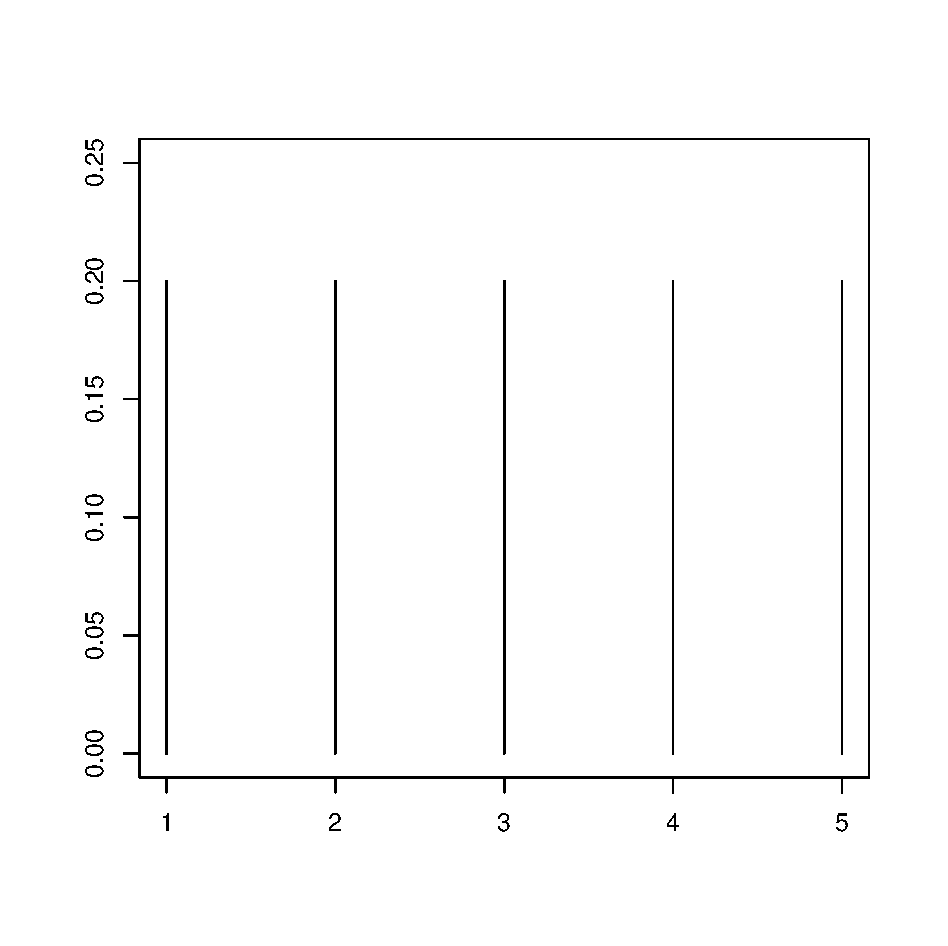
\includegraphics[scale=0.45]{Uniforme.eps}
\caption[\textsl{Densidad de una distribuci�n uniforme discreta sobre $\{1,\cdots,5\}$}]{\textsl{Funci�n de densidad de una distribuci�n uniforme discreta sobre $\{1,\cdots,5\}$.}}
\end{figure}

Esta distribuci�n describe situaciones donde el experimento aleatorio puede tener un finito de resultados, y la probabilidad de ocurrencia la misma para cada posible resultado. Entre los ejemplos de la distribuci�n uniforme discreta en la vida pr�ctica est�n el resultado (cara o sello) del lanzamiento de una moneda corriente, el resultado del lanzamiento de un dado corriente, resultado al extraer una bola al azar de una urna que contiene bolas enumeradas de 1 a $N$. Tambi�n en las rifas, donde en una bolsa que contiene, digamos, 145 nombres de los empleados de una empresas, al seleccionar un nombre de la bolsa para ser ganador de un computador port�til, la probabilidad de que Juan G�mez sea el ganador es $1/145$, y es claro que entre menos empleados hayan en la empresa, m�s probable es que Juan G�mez sea el ganador. Ahora, suponga que de las 145 empleados, hay 60 mujeres y 85 hombres (donde las 60 mujeres se denotan por M1, M2, $\cdots$, M60), entonces la probabilidad de que el ganador sea mujer puede ser pensada como la probabilidad de que el ganador sea M1, o sea M2, o $\cdots$, o M60. Recurriendo a propiedades de la probabilidad, se tiene que la probabilidad requerida ser� $1/145+1/145+\cdots+1/145$, 60 veces, esto es, $60/145$. M�s adelante, se ver� que la anterior situaci�n tambi�n puede ser descrita por una variable con distribuci�n hipergeom�trica.

En la vida pr�ctica, para identificar variables con distribuci�n uniforme discreta, en muchos casos basta con conocer el contexto del problema, es decir, con conocer condiciones que garantizan que los valores ocurren con la misma probabilidad, como por ejemplo, en el lanzamiento de una moneda, saber que la moneda no est� cargada garantiza que los resultados siguen esta distribuci�n. Sin embargo, puede suceder que se desconoce si esta condici�n se tiene o no, y lo disponible es simplemente un conjunto de valores. Suponga que se tienen los valores, 3, 1, 3, 4, 2, 4, 2, 2, 1, 3 que denotan resultados de 10 selecciones de una bolsa con bolas enumeradas de 1 hasta 5. Dada la caracter�stica de la distribuci�n uniforme discreta, afirmar que el resultado de selecci�n tiene distribuci�n uniforme discreta es equivalente a afirmar que el proceso de selecci�n es completamente al azar, sin ninguna preferencia de n�meros. Ahora, si los datos provinieran de una distribuci�n uniforme sobre $\{1,\cdots,N\}$, entonces la probabilidad de ocurrencia de cualquier $n=1,\cdots,N$ debe ser igual a $1/N$. Haciendo la analog�a entre la probabilidad de ocurrencia con la frecuencia relativa que se puede ver en la Figura 1.2, podemos intuir que s� se presenta una variable uniforme discreta si las frecuencias relativas para 1, $\cdots$, 5 son todos cercanos a $1/5=0.2$. Por lo tanto, del histograma de los datos, se observa que la frecuencia relativa del valor 5 est� muy alejada del valor 0.2, de donde se sospecha la afirmaci�n de que la selecci�n fue realizada completamente al azar, sin ninguna preferencia de n�meros.

\begin{figure}[!htb]
\centering
\includegraphics[bb=0 0 1104 1047, scale=0.19]{Uniforme_Hist.jpg}
\caption{\textsl{Histograma de los datos 3, 1, 3, 4, 2, 4, 2, 2, 1, 3.}}
\end{figure}

Para generar valores de una distribuci�n uniforme discreta, se puede usar el comando \verb"sample" con la opci�n \verb"replace=TRUE", el siguiente c�digo simula dos conjuntos de valores a partir de una distribuci�n uniforme discreta sobre $\{1,2,3\}$, con tama�o 500 y 1000, respectivamente, y grafica los dos histogramas. Estos dos histogramas se muestran en la Figura 1.3, donde podemos observar que las frecuencias de los valores parecen ser constantes. Especialmente cuando el tama�o es grande, no hay alg�n valor con una frecuencia muy grande o muy peque�a con respecto a otros valores.
\newpage
\begin{verbatim}
> set.seed(123)
> n<-c(500,1000)
> theta<-3
> par(mfrow=c(1,2))
> for(i in 1:length(n)){
+ a<-n[i]
+ hist(sample(theta,n[i],replace=TRUE),main="",xlab=a,
+    ylab="Frecuencia")
+ }
\end{verbatim}


\begin{figure}[!htb]
\centering
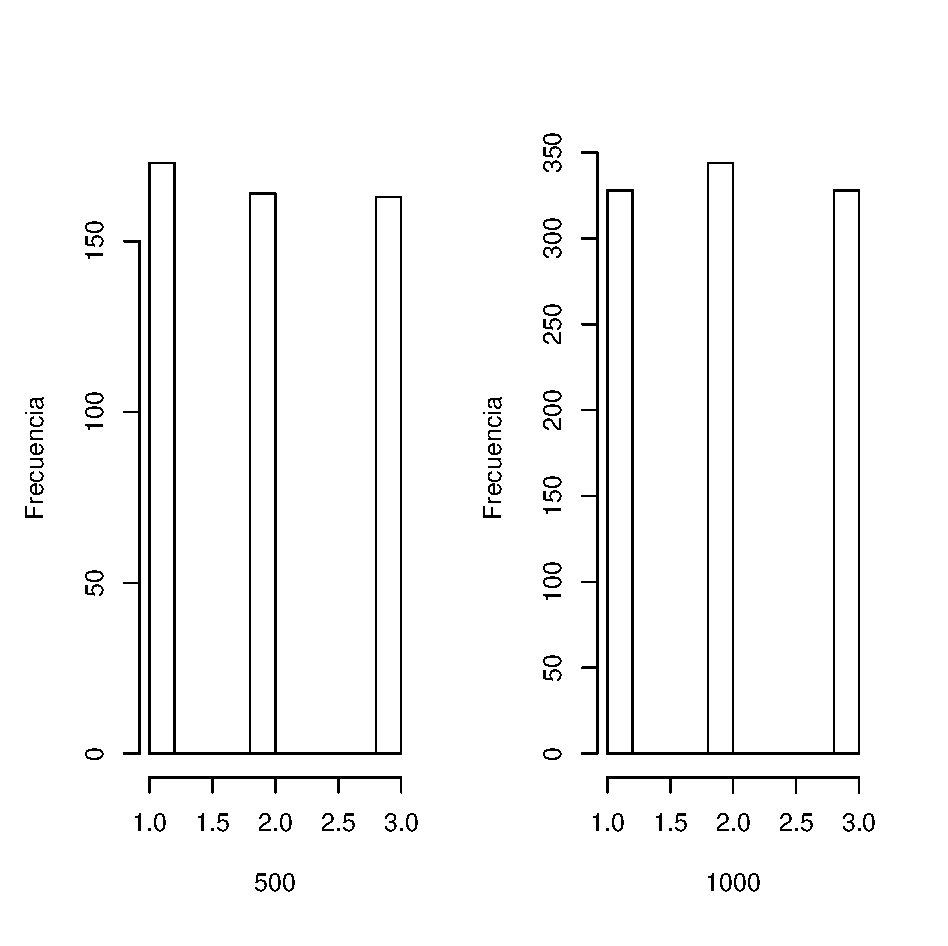
\includegraphics[scale=0.6]{random_unif.eps}
\caption[\textsl{Histograma de valores simulados de una distribuci�n uniforme}]{\textsl{Histograma de valores simulados de una distribuci�n uniforme discreta sobre $\{1,2,3\}$ con tama�o de muestra 500 y 1000.}}
\end{figure}

Algunas propiedades b�sicas de una distribuci�n uniforme se muestran a con\-ti\-nua\-ci�n.

\begin{Res}
Si $X$ es una variable aleatoria con distribuci�n uniforme discreta sobre el conjunto $\{1,2,\cdots,N\}$, entonces
    \begin{enumerate}
        \item $E(X)=\frac{N+1}{2}$.
        \item $Var(X)=\frac{N^2-1}{12}$.
        \item $m_X(t)=\sum_{i=1}^N\frac{e^{ti}}{N}$.
    \end{enumerate}
\end{Res}

\subsubsection{Distribuci�n Bernoulli\index{Distribuci�n!Bernoulli}}
La distribuci�n Bernoulli debe su nombre al matem�tico suizo Jacob Bernoulli (1654-1705). Esta distribuci�n es asociada con experimentos aleatorios que tienen solo dos posibles resultados, los cuales se etiquetan como \emph{�xito} y \emph{fracaso}, donde la probabilidad de obtener \emph{�xito} es $p$, con $0<p<1$. De esta forma una variable aleatoria que toma valor 1 cuando se observa el \emph{�xito} y 0 en el caso de \emph{fracaso} tiene distribuci�n Bernoulli con par�metro $p$. En la vida pr�ctica, se presentan muchos ensayos del tipo Bernoulli; por ejemplo, el �xito o fracaso de un correo electr�nico ofreciendo alg�n servicio o producto. En la teor�a del muestreo, la pertenencia de un elemento de la poblaci�n en la muestra tambi�n tiene distribuci�n Bernoulli.

\begin{figure}[!htb]
\centering
\includegraphics[bb=0 0 300 455, scale=0.25]{Bernoulli.jpg}
\caption{\textsl{Jacob Bernoulli (1654-1705)}}
\end{figure}

En t�rminos de la funci�n de densidad tenemos la siguiente definici�n de la distribuci�n Bernoulli .

\begin{Defi}
Una variable aleatoria $X$ tiene distribuci�n Bernoulli con par�metro $p\in (0,1)$ si su funci�n de densidad est� dada por:
\begin{equation}\label{densidad_Bernoulli}
f_X(x)=p^x(1-p)^{1-x}I_{\{0,1\}}(x),
\end{equation}
y se nota como $X\sim Ber(p)$.
\end{Defi}

N�tese que si $X\sim Ber(p)$, entonces $Pr(X=1)=p$, y $Pr(X=0)=1-p$. Y tenemos las siguientes propiedades para la distribuci�n Bernoulli.
\begin{Res}
Si $X$ es una variable aleatoria con distribuci�n Bernoulli con par�metro $p$, entonces
    \begin{enumerate}
        \item $E(X)=p$.
        \item $Var(X)=p(1-p)$.
        \item $m_X(t)=pe^t+1-p$.
    \end{enumerate}
\end{Res}

\begin{proof}
Las anteriores tres expresiones se pueden obtener f�cilmente usando la definici�n de la esperanza para una variable discreta. En particular, $m_X(t)=E(e^{tX})=e^{t}Pr(X=1)+e^{0}Pr(X=0)=pe^t+1-p$.
\end{proof}

En muchos casos, no se observa un solo ensayo del tipo Bernoulli, sino una series de ensayos. Por ejemplo, una empresa que hace ventas virtuales, no manda el correo de promocionamiento a una sola persona, sino a muchos, y la empresa est� interesada en cantidades como si se manda el mismo correo a 30 personas distintas, cu�ntas ventas exitosas obtendr�; es decir, estamos interesados en la variable definida como \emph{el n�mero de �xitos en $n$ ensayos del tipo Bernoulli}. Este tipo de variables se describen con la distribuci�n binomial que se estudiar� a continuaci�n.

\subsubsection{Distribuci�n binomial\index{Distribuci�n!binomial}}
\begin{Defi}
Una variable aleatoria $X$ tiene distribuci�n binomial con los pa\-r�\-me\-tros $n\in \mathbb{N}$ y $p\in (0,1)$ si su funci�n de densidad est� dada por:
\begin{equation}
f_X(x)=Pr(X=x)=\binom{n}{x}p^x(1-p)^{n-x}I_{\{0,1,\cdots,n\}}(x),
\end{equation}
y se nota como $X\sim Bin(n,p)$.
\end{Defi}

De acuerdo a lo discutido al final de la secci�n anterior, una aplicaci�n de la distribuci�n binomial es cuando tenemos un n�mero $n$ de repeticiones independientes de un mismo experimento del tipo Bernoulli, donde la probabilidad del �xito en cada ensayo se denota por $p$, entonces la variable \emph{n�mero de �xitos obtenidos en las $n$ repeticiones} tiene distribuci�n $Bin(n,p)$. Dada la anterior interpretaci�n, podemos ver f�cilmente que los valores que toma $X$ son enteros entre 0 y $n$, denotando el valor de 0 la situaci�n donde en todos los ensayos se obtuvo como resultado \emph{fracaso}, y el valor de $n$ cuando todos los ensayos tuvieron como resultado \emph{�xito}. En la Figura 1.5, se muestra la funci�n de densidad de una distribuci�n $Bin(10,0.35)$, donde se observa que a diferencia de la distribuci�n uniforme discreta, la distribuci�n binomial tiene un valor que tiene mayor probabilidad que otros, digamos $x_0$, y a medida que se aleja de $x_0$, la probabilidad disminuye, aunque no de la forma sim�trica.

\begin{figure}[!htb]
\centering
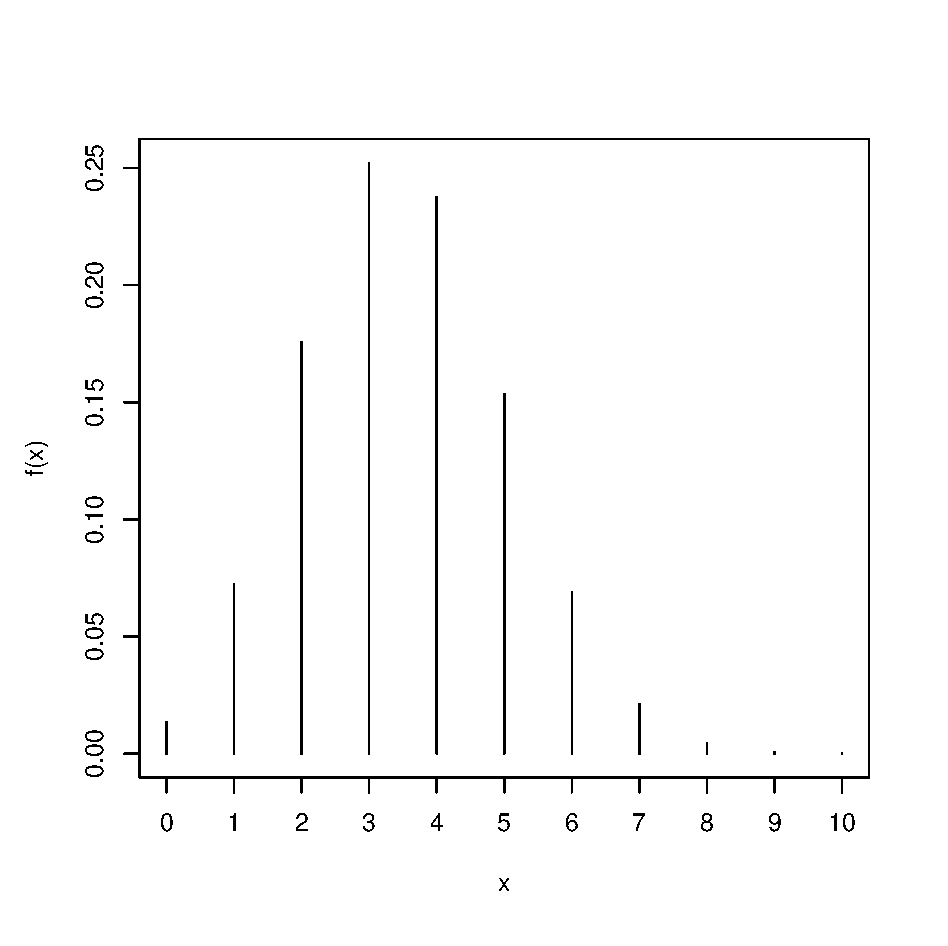
\includegraphics[scale=0.5]{densidad_binomial.eps}
\caption{\textsl{Funci�n de densidad de una distribuci�n $Bin(10,0.35)$.}}
\end{figure}

Esta distribuci�n tiene dos par�metros: $n$ y $p$. Sin embargo, en muchas aplicaciones en la vida pr�ctica el n�mero de repeticiones $n$ es conocido, y la distribuci�n depender� s�lo del valor $p$ que ser�a el par�metro de la distribuci�n con espacio param�trico $\bTheta=(0,1)$.

Algunas propiedades de la distribuci�n binomial se enuncian a continuaci�n.
\begin{Res}
Si $X$ es una variable aleatoria con distribuci�n binomial con pa\-r�\-me\-tros $n$ y $p$, entonces
    \begin{enumerate}
        \item $E(X)=np$.
        \item $Var(X)=np(1-p)$.
        \item $m_X(t)=(pe^t+1-p)^n$.
    \end{enumerate}
\end{Res}
\begin{proof}
Se deja como ejercicio (Ejercicio 1.4).
\end{proof}

\textbf{Observaci�n:} el lector puede verificar f�cilmente que la distribuci�n Bernoulli es un caso particular de la distribuci�n binomial cuando $n=1$. Y el Resultado 1.1.2 tambi�n se puede obtener del anterior resultado con $n=1$. Tambi�n podemos ver que en una distribuci�n binomial, el valor m�s probable est� cercano de la esperanza de la distribuci�n; por ejemplo, en la distribuci�n $Bin(10,0.35)$, la esperanza est� dada por 3.5, mientras que en la Figura 1.5 se observa que el valor m�s probable es 3. De all� podemos sacar conclusiones muy sencillas sin mayores c�lculos: por ejemplo, la empresa de ventas virtuales sabe por experiencia que la probabilidad de obtener una venta exitosa con un correo enviado es del 0.04, entonces si env�a 200 correos, lo m�s probable es que obtenga aproximadamente $0.04*200=8$ ventas.

La generaci�n de observaciones provenientes de una distribuci�n binomial puede realizarse mediante el comando \verb"rbinom"; de esta manera, si queremos simular 100 va\-lores provenientes de una distribuci�n $Bin(10,0.35)$, podemos usar el siguiente c�digo \verb"rbinom(1000,10,0.35)". El histograma de un conjunto de datos simulados con esta instrucci�n est� dado en la Figura 1.6, donde se observa un comportamiento muy similar a la funci�n de densidad te�rica dada en la Figura 1.5.

\begin{figure}[!htb]
\centering
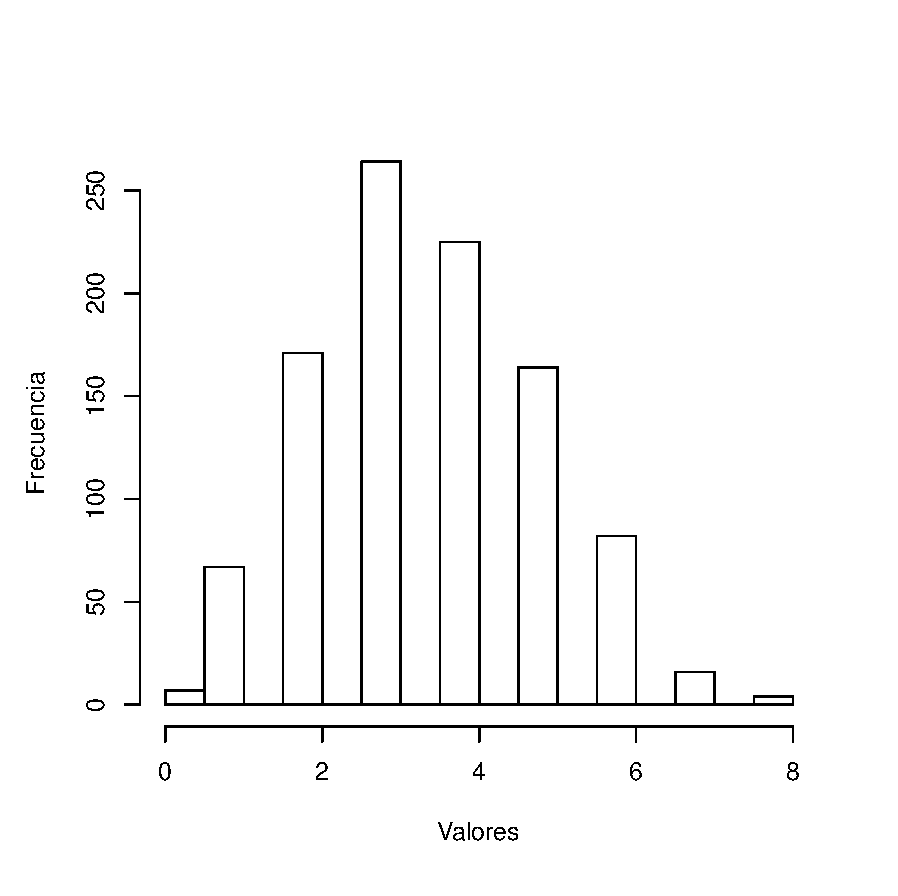
\includegraphics[scale=0.5]{hist_binomial.eps}
\caption{\textsl{Histograma de un conjunto de datos provenientes de $Bin(10,0.35)$.}}
\end{figure}


Usando la funci�n generadora de momentos del Resultado 1.1.3, podemos establecer el siguiente resultado que ilustra la relaci�n entre las distribuciones Bernoulli y binomial.

\begin{Res}
Sea $X_1$, $\cdots$, $X_n$ variables aleatorias independientes e id�nticamente distribuidas con distribuci�n Bernoulli con par�metro $p$,
entonces la variable $\sum_{i=1}^nX_i$ tiene distribuci�n $Bin(n,p)$.
\end{Res}
\newpage
\begin{proof}
La demostraci�n radica en el hecho de que la funci�n generadora de momentos caracteriza la distribuci�n probabil�stica, entonces basta demostrar que la funci�n generadora de momentos de $\sum_{i=1}^nX_i$ es la de una distribuci�n $Bin(n,p)$. Tenemos lo siguiente:
\begin{align*}
m_{\sum X_i}(t)=E(e^{\sum tX_i})&=E\left(\prod_{i=1}^ne^{tX_i}\right)\\
               &=\prod_{i=1}^nE(e^{tX_i})\ \ \ \ (\text{por independencia})\\
               &=\prod_{i=1}^n(pe^t+1-p)\ \ \ \ (\text{definici�n de $m_{X_i}(t)$})\\
               &=(pe^t+1-p)^n.
\end{align*}
Y el resultado queda demostrado.
\end{proof}

\subsubsection{Distribuci�n hipergeom�trica\index{Distribuci�n!hipergeom�trica}}
\begin{Defi}
Una variable aleatoria $X$ tiene distribuci�n hipergeom�trica con par�metros $n$, $R$ y $N$ si su funci�n de densidad est� dada por:
\begin{equation}
f_X(x)=Pr(X=x)=\frac{\binom{R}{x}\binom{N-R}{n-x}}{\binom{N}{n}},
\end{equation}
para $x$ entero entre $\max(n-N+R,0)$ y $\min(R,n)$, y se nota como $X\sim Hg(n,R,N)$.
\end{Defi}

Una variable con distribuci�n hipergeom�trica se da cuando se desea extraer $n$ unidades de un conjunto de $N$ objetos en total, que se pueden dividir en dos grupos: el primero de $R$ unidades y el segundo de $N-R$. Entonces la variable definida como el n�mero de unidades extra�das del primer grupo tiene distribuci�n hipergeom�trica con par�metros $n$, $R$ y $N$. Suponga que se desea extraer 6 estudiantes de 15 en total, donde 10 son hombres y 5 son mujeres; la variable $X$ definida como \emph{el n�mero de estudiantes hombres seleccionados} tiene distribuci�n $Hg(6,10,15)$. N�tese que $X$ solo toma valores entre 1 y 6, puesto que al seleccionar 6 estudiantes, a lo m�s 5 mujeres pueden quedar en la muestra, es decir, por lo menos estar�n en la muestra. En la Figura 1.7, se muestra la funci�n de densidad para esta distribuci�n.

\begin{figure}[!htb]
\centering
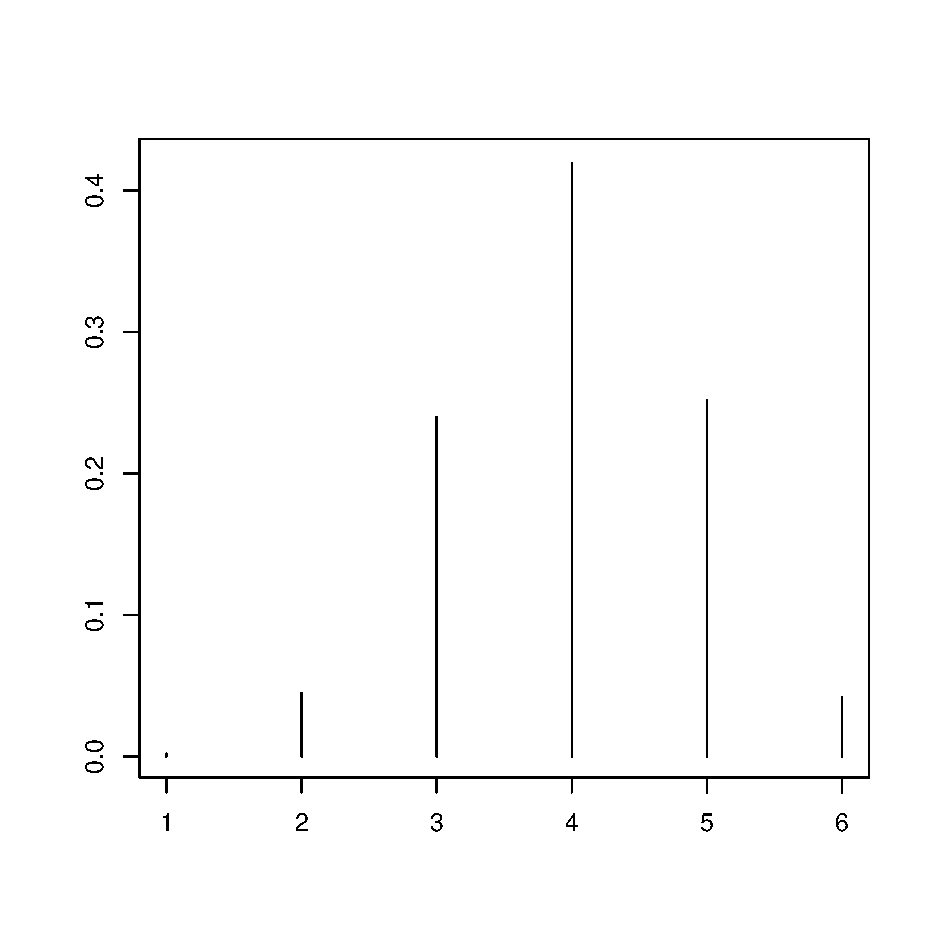
\includegraphics[scale=0.45]{hipergeometrica.eps}
\caption{\textsl{Funci�n de densidad de una distribuci�n $Hg(6,10,15)$.}}
\end{figure}

Algunas propiedades de la distribuci�n hipergeom�trica se enuncian a continuaci�n.

\begin{Res}
Si $X$ es una variable aleatoria con distribuci�n hipergeom�trica con par�metros $n$, $R$ y $N$, entonces
    \begin{enumerate}
        \item $E(X)=\frac{nR}{N}$.
        \item $Var(X)=\frac{nR(N-R)(N-n)}{N^2(N-1)}$.
    \end{enumerate}
\end{Res}

El anterior resultado no incluye la funci�n generadora de momentos, pues �ste no ha resultado ser �til en la teor�a relacionada con la distribuci�n hipergeom�trica.

La distribuci�n hipergeom�trica tambi�n es �til en la teor�a de muestreo, tal como ilustran \citeasnoun{Tille}, al considerar una regi�n agricultural que consiste en $N=2010$ fincas de donde se desea extraer una muestra aleatoria simple sin reemplazo de tama�o $n=100$. N�tese que cada elemento de la poblaci�n tiene la misma probabilidad de pertenecer a la muestra y puede ser seleccionado a lo m�s una vez. Suponga que adicionalmente se dispone la informaci�n sobre el �rea total cultivada de cada finca, de donde se sabe que en la poblaci�n total existen 1580 fincas de menos de 160 hect�reas (subgrupo 1) y 430 de m�s de 160 hect�reas (subgrupo 2). Aunque el tama�o muestral $n$ est� fijo, el n�mero de fincas del subgrupo 1 seleccionadas denotado por $n_1$ es aleatorio y sigue una distribuci�n $Hg(100,1580,2010)$; tambi�n el n�mero de fincas del subgrupo 2 seleccionadas $n_2$ sigue una distribuci�n hipergeom�trica $Hg(100,430,2010)$.

Usando el resultado anterior, podemos obtener que $E(n_1)=100\times1580/2010=78.6$, esto es, se espera seleccionar 78 o 79 fincas del subgrupo 1.

Otro uso de la distribuci�n hipergeom�trica es el problema de captura-recaptura, donde se necesita estimar el tama�o de una poblaci�n de inter�s. Para ello, se identifica un n�mero $R$ menor que $N$ de individuos, luego se deja que estos $R$ individuos se mezclen bien con el resto de la poblaci�n. Despu�s de esto, se selecciona $n$ individuos de la mezcla homog�nea, y se cuenta el n�mero, $x$, de individuos marcados que quedaron seleccionados. Dado que la poblaci�n estaba homog�nea al momento de la selecci�n, podemos pensar que las proporciones de objetos marcados en la muestra y en la poblaci�n deben ser similares, esto es,

\newpage

\begin{equation}\label{captura}
\frac{x}{n}\approx\frac{R}{N},
\end{equation}

de donde se tiene que $N\approx nR/x$. Para una ilustraci�n de este escenario, ver Figura 1.8. Otra aplicaci�n de la distribuci�n hipergeom�trica es cuando se desea estimar el tama�o de un subgrupo de una poblaci�n conocida, el procedimiento es el mismo de la captura recaptura, y se tiene la relaci�n de (\ref{captura}), de donde se tiene que $R\approx xN/n$. Suponga que en una ciudad existen 2396 empresas que pueden clasificar en empresas grandes, medianas o peque�as seg�n el n�mero de empleados. Si en una muestra aleatoria simple sin reemplazos de tama�o 200 se encuentran 28 empresas grandes, podemos estimar el n�mero total de empresas grandes en la poblaci�n total como $28*2396/200\approx335$ empresas grandes. M�s detalles sobre la estimaci�n en las anteriores situaciones se describen en el siguiente cap�tulo.

\begin{figure}[!htb]
\centering
\includegraphics[bb=0 0 1400 899, scale=0.14]{Captura_Recaptura.jpg}
\caption{\textsl{Ilustraci�n del problema de captura recaptura.}}
\end{figure}

N�tese que un experimento del tipo hipergeom�trico est� muy relacionado con un experimento Bernoulli, puesto que en la $i$-�sima extracci�n para $i=1,\cdots,n$, podemos definir $X_i$ como 1 si el resultado es uno de los $R$ objetos y 0 si no. De esta forma, tenemos $n$ variables con distribuci�n Bernoulli, y la variable $Hg(n,R,N)$ viene siendo la variable $X=X_1+\cdots+X_n$. Aunque las variables $X_1$, $\cdots$, $X_n$ son del tipo Bernoulli, no podemos afirmar que $X$ tiene distribuci�n binomial, puesto que dado el mecanismo de selecci�n, estas $n$ variables no son independientes. Sin embargo, bajo algunas condiciones, s� podemos afirmar que una distribuci�n hipergeom�trica puede ser aproximada como una distribuci�n binomial, tal como lo afirma el siguiente resultado.

\begin{Res}
Dada una variable aleatoria $X$ con distribuci�n $Hg(n,R,N)$, si se tiene que $R/N\rightarrow p$, con $0<p<1$ cuando $R,N\rightarrow\infty$, entonces, la funci�n de densidad de $X$ tiende a la funci�n de densidad de una distribuci�n $Bin(n,p)$.
\end{Res}

Para estudiar la convergencia enunciada en el anterior resultado, se calcul� la funci�n de densidad de cuatro distribuciones hipergeom�tricas con diferentes valores de $R$ y $N$, y las respectivas distribuci�n $Bin(n,R/N)$. El c�digo de R es como sigue y la gr�fica arrojada se muestra en la Figura 1.9. Podemos observar de la gr�fica resultante que la aproximaci�n por medio de la distribuci�n binomial puede ser muy adecuada para valores grandes de $R$ y $N$.


\begin{figure}[!htb]
\centering
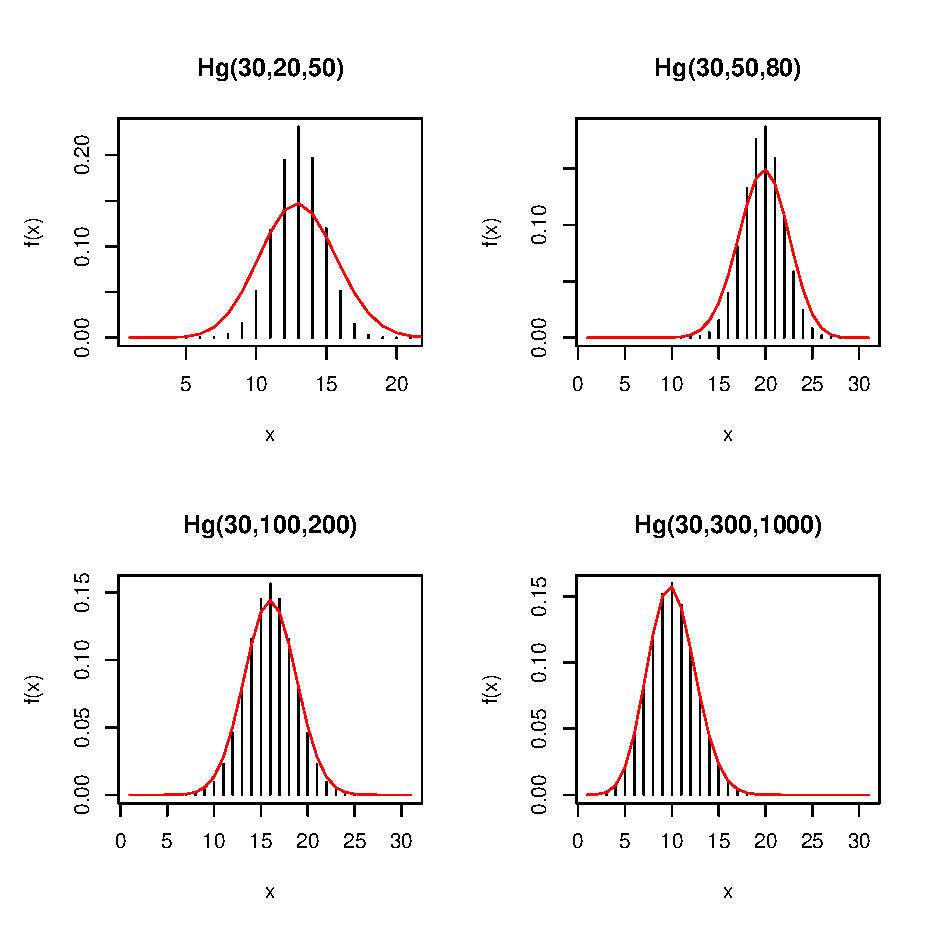
\includegraphics[scale=0.6]{hiper_binomial.eps}
\caption[\textsl{Aproximaci�n de la distribuci�n hipergeom�trica mediante la binomial}]{\textsl{Ilustraci�n de la aproximaci�n de la distribuci�n hipergeom�trica mediante la distribuci�n binomial. (L�nea roja indica la correspondiente distribuci�n binomial)}}
\end{figure}

\begin{verbatim}
> Hg<-function(x,n,R,N){
+ x<-c(max(0,n-N+R):min(R,n))
+ res<-rePr(NA,length(x))
+ for(i in 1:length(x)){
+ res[i]<-choose(R,x[i])*choose(N-R,n-x[i])/choose(N,n)}
+ return(res)
+ }
>
> par(mfrow=c(2,2))
>
> plot(Hg(x,30,20,50),type="h",main="Hg(30,20,50)",xlab="x",
+  ylab="f(x)")
> lines(dbinom(x,n,20/50),col=2)
>
> plot(Hg(x,30,50,80),type="h",main="Hg(30,50,80)",xlab="x",
+  ylab="f(x)")
> lines(dbinom(x,n,50/80),col=2)
> plot(Hg(x,30,100,200),type="h",main="Hg(30,100,200)",xlab="x",
+  ylab="f(x)")
> lines(dbinom(x,n,100/200),col=2)
>
> plot(Hg(x,30,300,600),type="h",main="Hg(30,300,600)",xlab="x",
+  ylab="f(x)")
> lines(dbinom(x,n,300/600),col=2)
\end{verbatim}

Volviendo al problema de la selecci�n de una muestra con $n=100$ de fincas que se dividen en dos grupos, podemos aproximar la variable aleatoria $n_1$ con una distribuci�n $Bin(100,1580/2010)$, y de esta forma calcular probabilidades acerca de los posibles valores de $n_1$.

\subsubsection{Distribuci�n Poisson\index{Distribuci�n!Poisson}}
La distribuci�n Poisson debe su nombre al franc�s Sim�on-Denis Poisson (1781-1840), quien descubri� esta distribuci�n en el a�o 1838, cuando la us� para describir el n�mero de ocurrencias de alg�n evento durante un intervalo de tiempo de longitud dada. Como de costumbre, damos la definici�n de esta distribuci�n en t�rminos de la funci�n de densidad.

\begin{figure}[!htb]
\centering
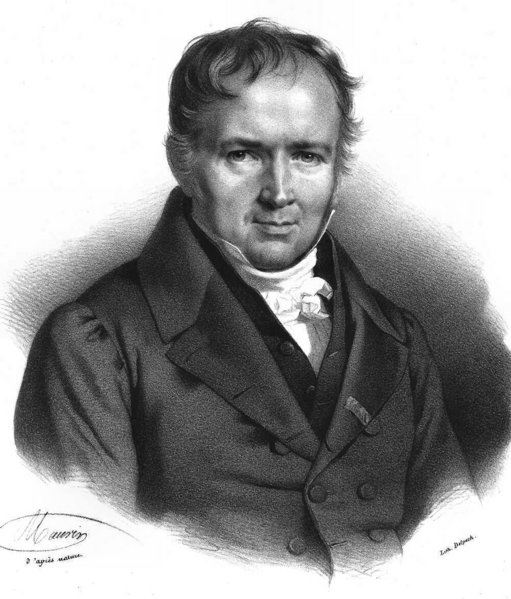
\includegraphics[bb=0 0 511 599, scale=0.27]{Poisson.jpg}
\caption{\textsl{Sim�on-Denis Poisson (1781-1840)}}
\end{figure}

\begin{Defi}
Una variable aleatoria $X$ tiene distribuci�n Poisson con par�metros $\lambda>0$ si su funci�n de densidad est� dada por:
\begin{equation}
f_X(x)=Pr(X=x)=\frac{e^{-\lambda}\lambda^x}{x!}I_{\{0,1,\cdots\}}(x)
\end{equation}
y se nota como $X\sim Pois(\lambda)$.
\end{Defi}

La funci�n de densidad de una distribuci�n Poisson presenta un pico en valores cercanos al par�metro $\lambda$. En la Figura 1.11, se ilustra la densidad de una distribuci�n $Pois(5.5)$, donde se observa que el valor con mayor probabilidad corresponde al valor 5, y a medida que el valor de $x$ se aleja de 5, las probabilidades disminuyen.

\begin{figure}[!htb]
\centering
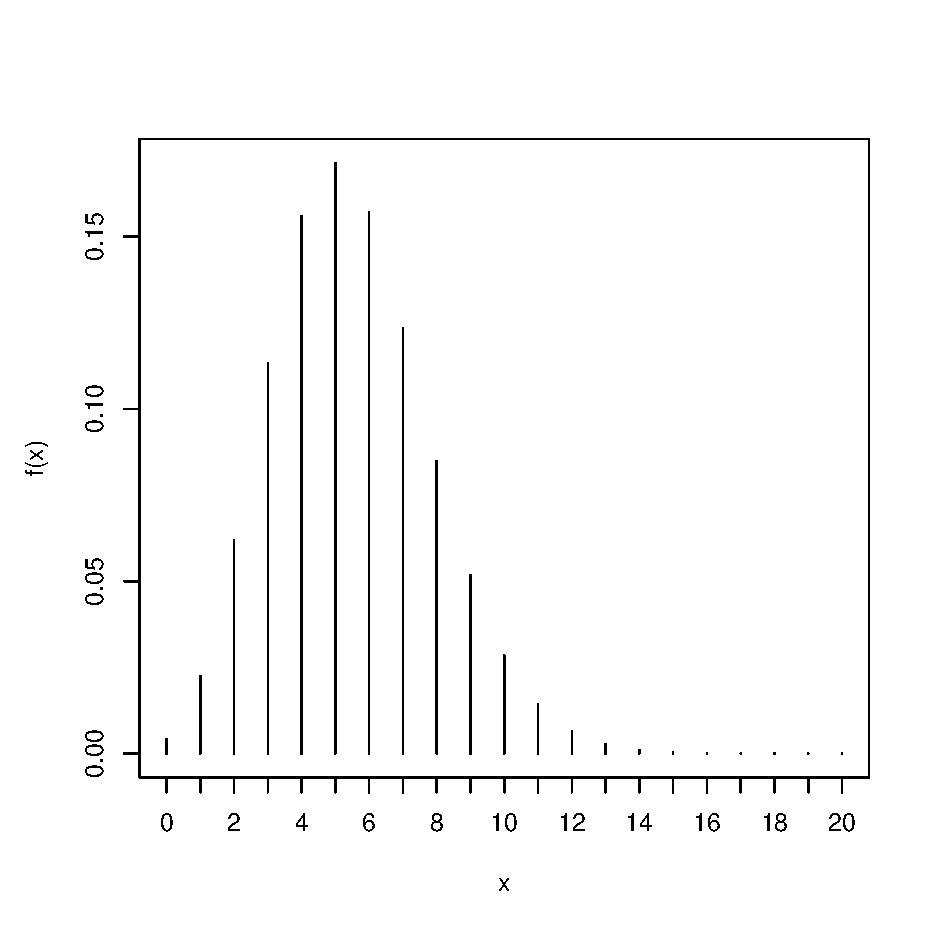
\includegraphics[scale=0.5]{densidad_poisson.eps}
\caption{\textsl{Funci�n de densidad de una distribuci�n $Pois(5)$.}}
\end{figure}

N�tese que una variable con distribuci�n Poisson puede tomar cualquier valor entero no negativo, y por esta raz�n, es usada frecuentemente para describir datos de conteo. Cuando en la pr�ctica se presentan un conjunto de valores que son conteos, debe tener en cuenta la diferencia entre las distribuciones binomial, hipergeom�trica y Poisson. En primer lugar, los valores que toma una variable con distribuci�n Poisson no debe tener un l�mite superior, es decir, puede ser cualquier entero positivo. Por lo tanto, contextos donde la variable en cuesti�n no puede ser m�s grande que alg�n valor no deben ser considerados como una variable Poisson. En segundo lugar, tanto la distribuci�n binomial como la hipergeom�trica, la variable puede ser vista como un n�mero de �xito obtenido en una sucesi�n de ensayos, mientras que la distribuci�n Poisson carece de esta interpretaci�n. De esta forma, una variable que describe, por ejemplo, n�mero de accidentes automovil�sticos en una determinada localidad, n�mero de transacciones en una entidad durante diez minutos, o en general, n�mero de eventos ocurridos en un punto geogr�fico y/o en un determinado rango del tiempo puede ser vista como una variable con distribuci�n Poisson.

Por otro lado, aunque una variable con distribuci�n Poisson solo toma valores enteros, el par�metro de la distribuci�n puede ser cualquier n�mero real positivo, esto es, el espacio param�trico de la distribuci�n es $\bTheta=(0,\infty)$.

\newpage

Ahora bien cuando no se puede conocer la procedencia de un conjunto de los datos, podemos utilizar el histograma de �stos para identificar la distribuci�n de donde provienen, puesto que el histograma debe ser similar a la densidad te�rica de la distribuci�n. Considere el siguiente ejercicio: en R, la generaci�n de n�meros aleatorios puede ser llevada a cabo usando el comando \verb"rpois". En la Figura 1.12, se muestra el histograma de 300 datos provenientes de la distribuci�n $Pois(5.5)$ generados usando la instrucci�n \verb"rpois(300,5.5)". Podemos observar que el histograma tiene un comportamiento muy similar a la funci�n de densidad te�rica de la distribuci�n, presentando mayor frecuencia en el valor 5 y comportamiento decreciente para valores alejados de 5.

\begin{figure}[!htb]
\centering
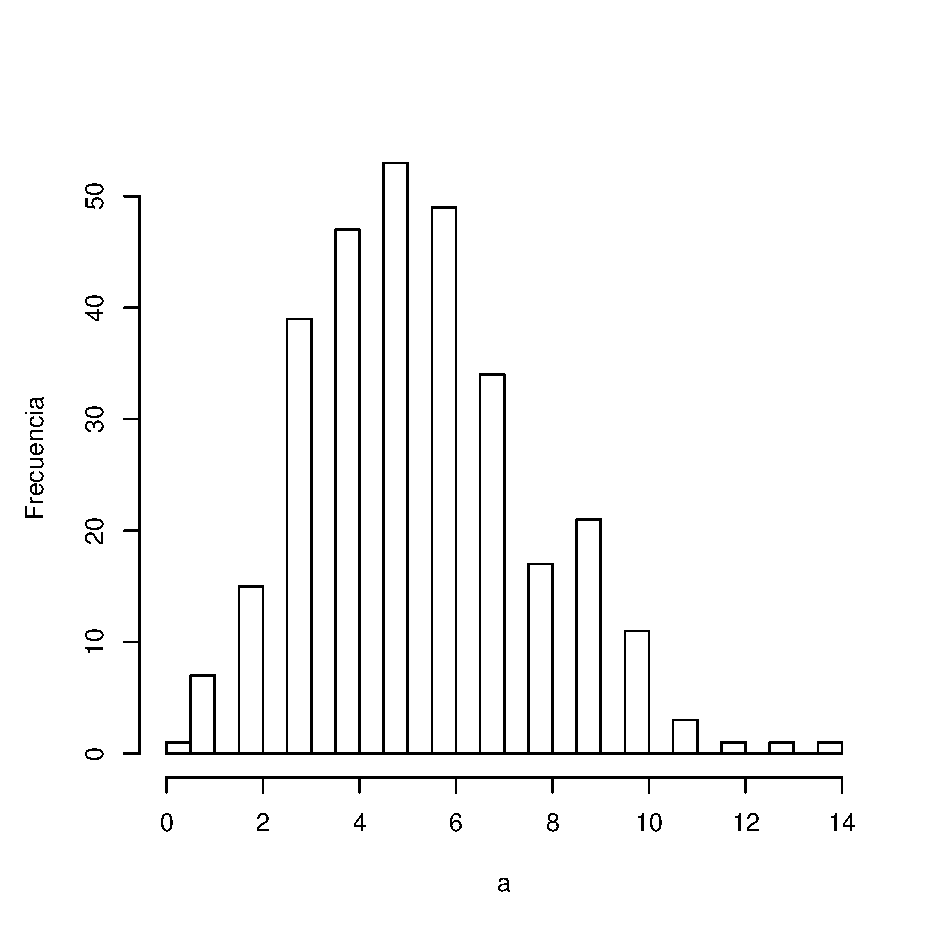
\includegraphics[scale=0.5]{hist_poisson.eps}
\caption{\textsl{Histograma de un conjunto de datos provenientes de $Pois(5.5)$.}}
\end{figure}

Algunas propiedades de la distribuci�n Poisson se enuncian a continuaci�n:

\begin{Res}
Si $X$ es una variable aleatoria con distribuci�n Poisson con par�metro $\lambda$, entonces
    \begin{enumerate}
        \item $E(X)=\lambda$.
        \item $Var(X)=\lambda$.
        \item $m_X(t)=\exp\{\lambda(e^t-1)\}$.
    \end{enumerate}
\end{Res}

\begin{proof}
La demostraci�n del anterior resultado se deja como ejercicio (Ejercicio 1.6) y consiste en encontrar la funci�n generadora de momentos, $m_X(t)$, usando directamente su definici�n y la expansi�n de Tayler de $e^u$ dada por $e^u=\sum_{i=0}^{\infty}\frac{u^i}{i!}$. Una vez encontrada $m_X(t)$, se encuentra la esperanza y la varianza de manera habitual.
\end{proof}

El anterior resultado, a parte de proveernos propiedades de la distribuci�n Poisson, tambi�n nos brinda una herramienta a la hora de identificar la distribuci�n de datos cuya procedencia no se conoce, puesto que de acuerdo al resultado anterior, si un conjunto de datos proviene de la distribuci�n Poisson, entonces el promedio debe ser cercano a la varianza; m�s a�n, el promedio y la varianza deben ser cercanos al par�metro de la distribuci�n. En la pr�ctica, una distribuci�n que puede ser confundida con la distribuci�n Poisson es la distribuci�n binomial, puesto que ambas toman valores enteros positivos, pero en la distribuci�n Binomial, la varianza te�rica est� dada por $np(1-p)$, la cual es siempre menor que la esperanza $np$, situaci�n que no ocurre si se tratara de una distribuci�n Poisson.

Para corroborar la anterior afirmaci�n en la pr�ctica, se simularon muestras de tama�o 10, 30, 50, 100, 300, 500 y 1000 que provienen de la distribuci�n $Pois(5)$ y $Bin(20,0.25)$, y en cada muestra se calcul� el promedio y la varianza, el c�digo en R es como sigue, y tiene como resultado la Figura 1.13, donde podemos observar que en las muestras con distribuci�n Poisson, la varianza muestral se asemeja al promedio muestral, mientras que en las muestras con distribuci�n binomial, la varianza siempre estuvo por debajo del promedio con una diferencia considerable, corroborando las propiedades te�ricas. De lo anterior, podemos concluir que en un conjunto de datos, si la varianza es muy similar al promedio, hay m�s evidencia a favor de la distribuci�n Poisson que la binomial; mientras que si la varianza es considerablemente menor que el promedio, se puede decir que la distribuci�n binomial ajusta mejor a los datos\footnote{En otras distribuciones como la distribuci�n binomial negativa la varianza es m�s grande que la esperanza, y se denomina este fen�meno como la sobredispersi�n.}.

\begin{verbatim}
> set.seed(1234)
>
> n<-c(10,30,50,100,300,500,1000)
> mp<-matrix(NA)
> vp<-matrix(NA)
>
> for(i in 1:length(n)){
+ a<-rpois(n[i],5)
+ mp[i]<-mean(a)
+ vp[i]<-var(a)
+ }
>
> #####################
> mb<-matrix(NA)
> vb<-matrix(NA)
>
> for(i in 1:length(n)){
+ b<-rbinom(n[i],20,5/20)
+ mb[i]<-mean(b)
+ vb[i]<-var(b)
+ }
>
> par(mfrow=c(2,1))
>
> plot(mp,type="b",ylim=c(0,7),ylab="",xaxt="n",xlab="n",
+  main="Poisson(5)")
> lines(vp,type="b", pch=4)
> axis(1,1:length(n),n)
> legend("bottomright",c("Promedio","Varianza"), pch=c(1,4),bty="n")
>
> plot(mb,type="b",ylim=c(0,7),ylab="",xaxt="n",xlab="n",
+  main="Binomial(20,0.25)")
> lines(vb,type="b", pch=4)
> axis(1,1:length(n),n)
> legend("bottomright",c("Promedio","Varianza"), pch=c(1,4),bty="n")
\end{verbatim}

\begin{figure}[!htb]
\centering
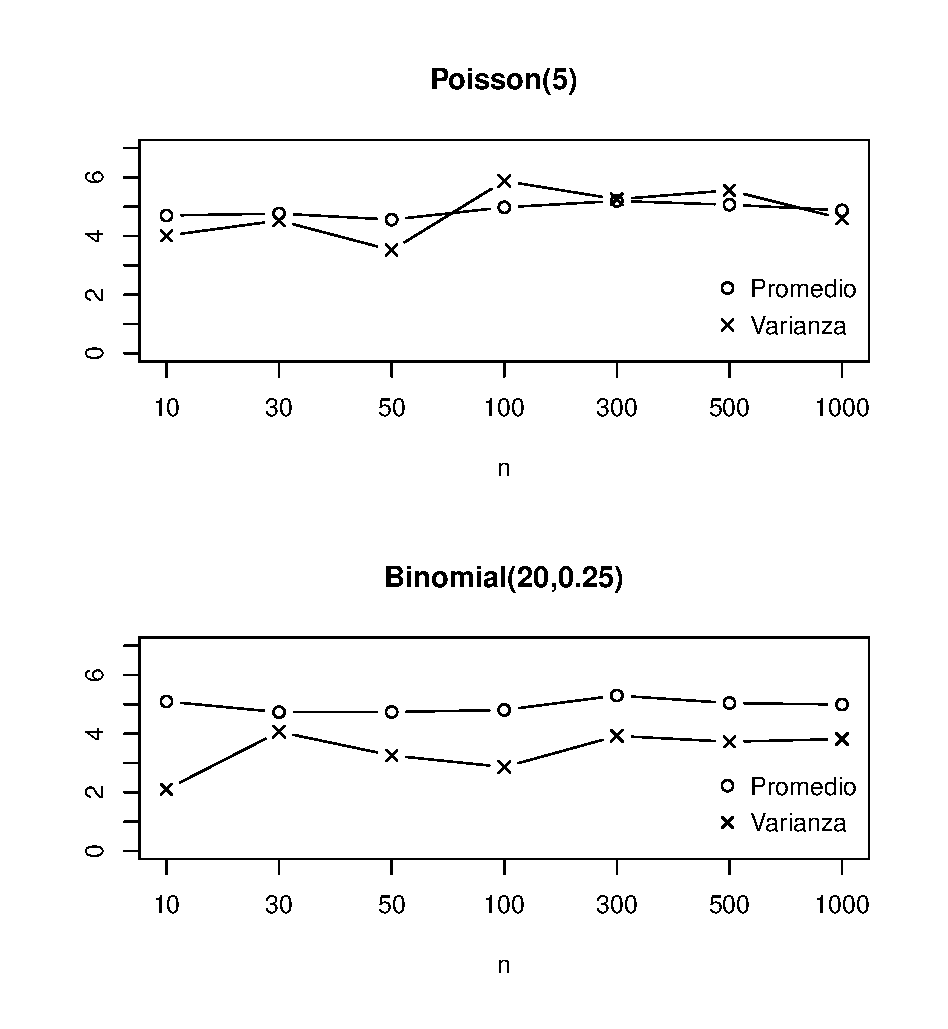
\includegraphics[scale=0.7]{poisson_binomial.eps}
\caption[\textsl{Media y varianza de muestras de $Pois(5.5)$ y $Bin(20,0.25)$}]{\textsl{Promedio y varianza de muestras provenientes de distribuciones $Pois(5.5)$ y $Bin(20,0.25)$.}}
\end{figure}

\newpage

Como se mencionaba anteriormente, en la pr�ctica, si no se conoce la procedencia de los datos, sino solo los valores, unos datos provenientes de la distribuci�n Poisson podr�an confundirse con la distribuci�n binomial. El siguiente resultado nos plantea una relaci�n entre estas dos distribuciones bajo algunas circunstancias especiales.

\begin{Res}
Considera $n$ eventos del tipo Bernoulli, donde $p$ denota la proba\-bi\-li\-dad del �xito de cada uno de los $n$ eventos. Si el valor de $p$ es peque�o y $np\rightarrow\lambda>0$ cuando $n\rightarrow\infty$, entonces la variable $X$ con distribuci�n $Bin(n,p)$ se distribuye aproximadamente con distribuci�n $Pois(\lambda)$.
\end{Res}

\begin{proof}
\citeasnoun[p. 114]{Liliana}.
\end{proof}

\begin{figure}[!htb]
\centering
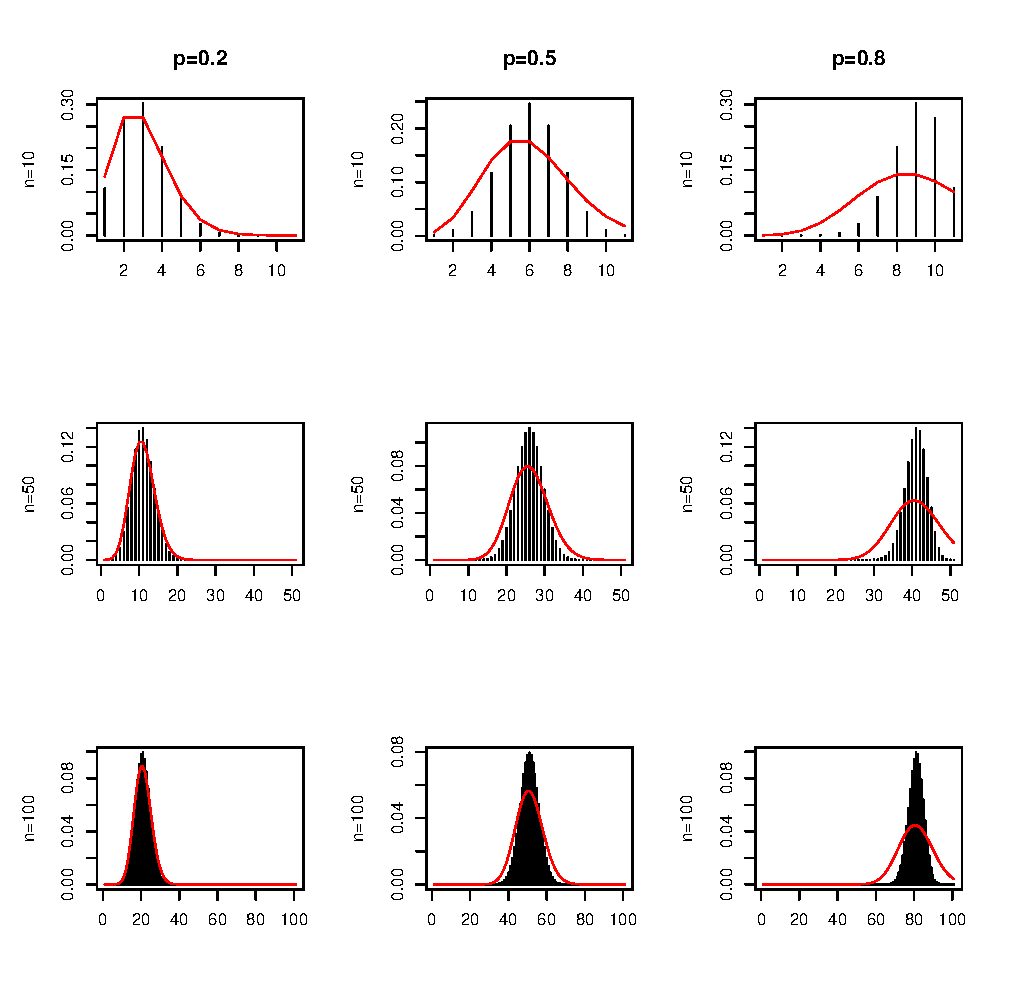
\includegraphics[scale=0.75]{binomial_poisson.eps}
\caption[\textsl{Aproximaci�n de la distribuci�n Poisson mediante la binomial}]{\textsl{Ilustraci�n de la aproximaci�n de la distribuci�n Poisson mediante la distribuci�n binomial del Resultado 1.1.8. (La l�nea gris indica la correspondiente distribuci�n Poisson)}}
\end{figure}

En el anterior resultado, existen dos condiciones para garantizar la convergencia, la probabilidad de �xito en cada ensayo $p$ debe ser peque�a y el n�mero de ensayos $n$ debe ser grande. Para hacerse una idea sobre qu� tan importantes son estas dos condiciones, se elabor� la Figura 1.14, la cual ilustra funciones de densidad de distribuci�n binomial con diferentes valores de $n$ y de $p$, y tambi�n la correspondiente distribuci�n Poisson. Se observa que efectivamente, a medida que aumenta el valor de $p$, la aproximaci�n se torna cada vez m�s mala, sin importar el tama�o muestral $n$. Por otro lado, se observa que la condici�n de que $p$ sea peque�a es m�s importante que la condici�n de que $n$ sea grande, puesto que para la distribuci�n $Bin(10,0.2)$, aunque $n$ sea peque�a, la aproximaci�n sigue siendo buena.

Ahora, aunque en la Figura 1.14 se observ� que cuando $p$ es peque�a, la aproximaci�n por la distribuci�n Poisson resulta no adecuada, podemos transformar a una variable $X\sim Bin(n,p)$ con $p$ grande para que siga siendo la v�lida la aproximaci�n. En este caso, es f�cil ver que la variable $Y=n-X\sim Bin(n,1-p)$, si $p$ es grande, $1-p$ es peque�o, entonces para calcular $f_X(x)=Pr(X=x)$, tenemos que �sta es igual a $Pr(Y=n-x)$, y utilizando la distribuci�n Poisson para aproximar la distribuci�n de $Y$ tenemos que
\begin{equation*}
Pr(X=x)=Pr(Y=n-x)\approx \frac{e^{-\lambda}\lambda^{n-x}}{(n-x)!},
\end{equation*}

con $\lambda=n(1-p)$. En la Figura 1.15, se ilustra la bondad de la anterior aproximaci�n para densidades de la distribuci�n binomial con distintos valores de $p$ y $n$, se observa que la aproximaci�n es bastante buena para valores grandes de $p$, mientras que cuando $p$ toma un valor cercano al 0.5, la anterior aproximaci�n es muy similar a la presentada en el Resultado 1.1.8.

Una propiedad interesante de la distribuci�n Poisson es el hecho de que la suma de variables independientes con distribuci�n Poisson sigue teniendo la distribuci�n Poisson. Lo anterior lo afirma el siguiente resultado.

\begin{Res}
Sea $X_1$, $\cdots$, $X_n$ variables aleatorias independientes con distribuci�n $Pois(\lambda_i)$ para $i=1,\cdots,n$, entonces la variable $\sum_{i=1}^nX_i$ tiene distribuci�n $Pois(\sum_{i=1}^n\lambda_i)$.
\end{Res}
\begin{proof}
La demostraci�n es an�loga a la demostraci�n del Resultado 1.1.4 y se deja como ejercicio (Ejercicio 1.7).
\end{proof}

\begin{figure}[!h]
\centering
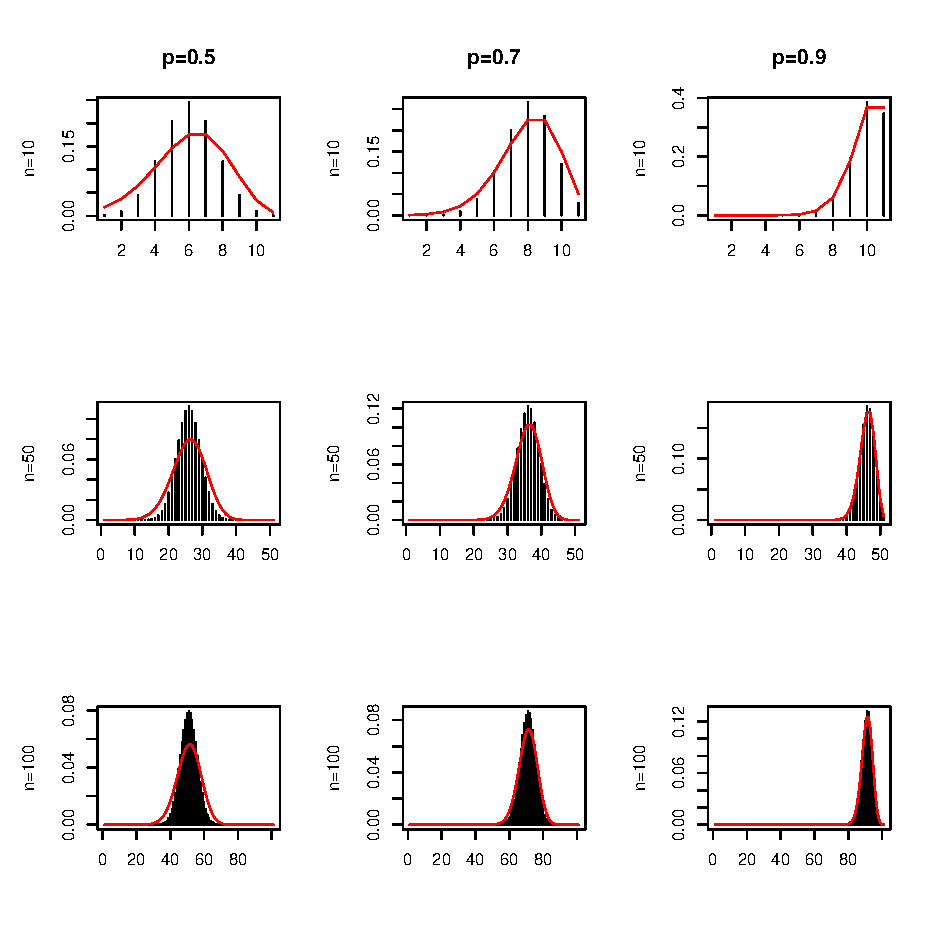
\includegraphics[scale=0.75]{binomial_poisson1.eps}
\caption[\textsl{Aproximaci�n de la distribuci�n Poisson mediante la binomial}]{\textsl{Ilustraci�n de la aproximaci�n de la distribuci�n Poisson mediante la distribuci�n binomial cuando $p$ es grande. (La l�nea gris indica la correspondiente distribuci�n Poisson)}}
\end{figure}

Suponga que una central telef�nica de atenci�n de clientes cuenta con 5 operadores en cada turno, la variable de inter�s es el n�mero de llamadas que atiende la central durante 5 minutos. Un estudio acerca del rendimiento de los 5 operadores de turno revela que el n�mero de llamadas que atiende en 5 minutos sigue una distribuci�n Poisson con par�metros 2, 3, 2, 4 y 3, respectivamente. Si adem�s los operadores trabajan de forma independiente, entonces el anterior resultado garantiza que el n�mero total de llamadas atendidas en 5 minutos puede ser modelado como una distribuci�n $Pois(14)$, y podemos calcular probabilidades acerca de esta variable de la manera habitual.

\subsection{Distribuciones continuas}
En esta parte del libro consideraremos las distribuciones continuas, esto es, algunas distribuciones comunes para variables aleatorias continuas.

\subsubsection{Distribuci�n Uniforme Continua\index{Distribuci�n!uniforme continua}}

Una de las distribuciones continuas m�s simples es la distribuci�n uniforme continua sobre un intervalo $[a,b]$, la cual se caracteriza en que para un subintervalo de $[a,b]$ de longitud fija, una variable con esta distribuci�n tiene la misma probabilidad de ubicarse en cualquiera de estos subintervalos. Por consiguiente, esta distribuci�n es apropiada para situaciones donde para un experimento no hay resultados que son m�s probables que otros, un aspecto similar a la distribuci�n uniforme discreta. De esta forma, si suponemos que el primer bus puede demorar a lo m�s 15 minutos para llegar al portal de transporte, y puede llegar en cualquier momento en ese rango, en este caso, la variable definida como el tiempo de llegada del bus tiene una distribuci�n uniforme $[0,15]$. Claramente el l�mite inferior 0 est� dado por el contexto del problema y la naturaleza de la variable.

La definici�n de esta distribuci�n en t�rminos de la funci�n de densidad est� dada a continuaci�n.

\begin{Defi}
Una variable aleatoria $X$ tiene distribuci�n uniforme continua sobre el intervalo $[a,b]$ con $a<b$ si su funci�n de densidad est� dada por:
\begin{equation}
f_X(x)=\frac{1}{b-a}I_{[a,b]}(x),
\end{equation}
y se denotar� por $X\sim U[a,b]$.
\end{Defi}

An�logo a lo discutido en la parte de la distribuci�n uniforme discreta, cuando los datos provienen de la distribuci�n $U[a,b]$, entonces el histograma debe ser plano, similar a la funci�n de densidad te�rica. Para observar lo anterior, simulamos dos muestras provenientes de la distribuci�n $U[1,3]$ del tama�o 500 y 1000 usando la instrucci�n \verb"runif", y graficamos los correspondientes histogramas. El c�digo usado es

\begin{verbatim}
set.seed(123)
n<-c(500,1000)
par(mfrow=c(1,2))
for(i in 1:length(n)){
a<-n[i]
hist(runif(a,1,3),main="",xlab=a,ylab="Frecuencia")
}
\end{verbatim}


\begin{figure}[!htb]
\centering
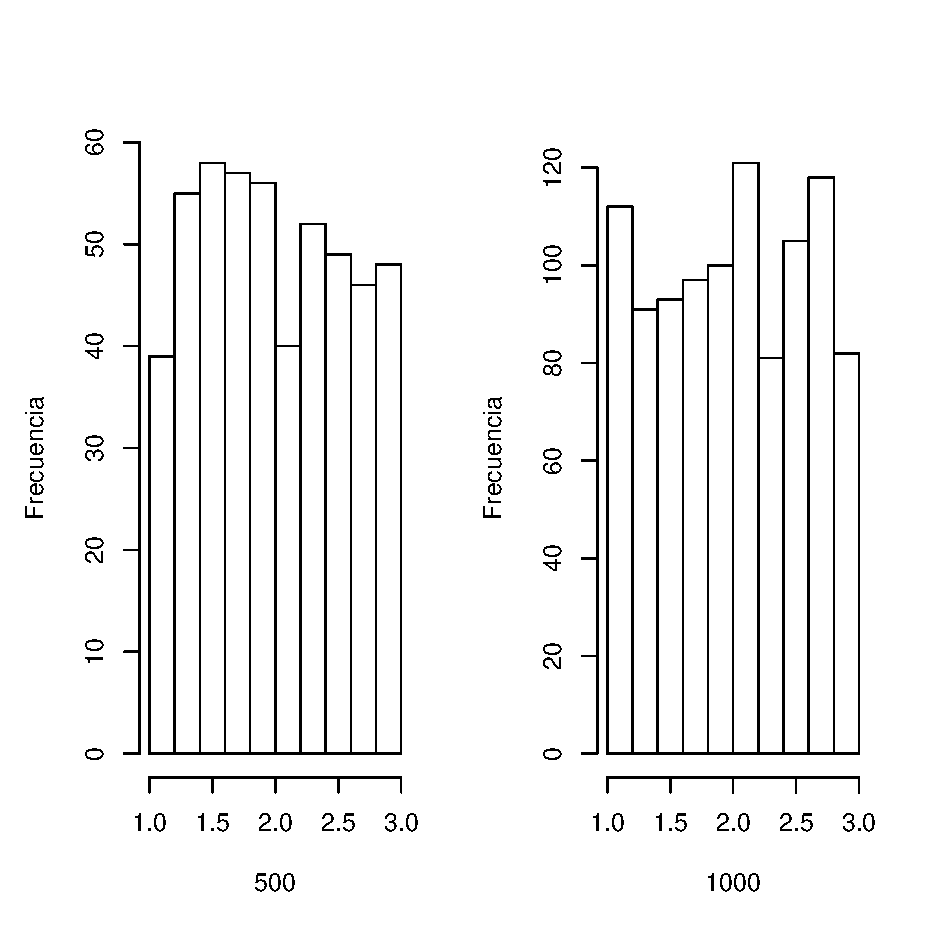
\includegraphics[scale=0.6]{random_unif_continua.eps}
\caption[\textsl{Histograma de valores simulados de una distribuci�n uniforme}]{\textsl{Histograma de valores simulados de una distribuci�n $U[1,3]$ con tama�o de muestra 500 y 1000.}}
\end{figure}

Y la resultante gr�fica est� dada en la Figura 1.16, donde se observa que efectivamente no hay alg�n patr�n reconocible en estos histogramas, sino que cada clase tiene aproximadamente la misma frecuencia, caracter�sticas propias de una distribuci�n uniforme continua.

La generaci�n de n�meros aleatorios de una distribuci�n $U[0,1]$ es particularmente importante, puesto que son de utilidad para simular otras distribuciones m�s complicadas que la distribuci�n uniforme. El procedimiento viene dado por el siguiente resultado tomado de \citeasnoun{Rober-Case}.
\begin{Res}
Si $U\sim U(0,1)$ y $F(x)$ es una funci�n de distribuci�n, entonces la funci�n de distribuci�n de la  variable $F^{-}(U)$ est� dada por $F$, donde $F^{-}$ denota la funci�n inversa generalizada de $F$ dada por $F^{-}(u)=\inf\{x:\ F(x)\geq u\}$.
\end{Res}
\newpage
El anterior resultado nos indica que si queremos simular $n$ valores a partir de una cierta distribuci�n $F$, se debe, en primer lugar, hallar la funci�n de distribuci�n inversa generalizada\footnote{Cuando la inversa de $F$ existe, �sta coincide con la inversa generalizada.} $F^{-}$, y en segundo lugar, simular $n$ observaciones de la distribuci�n $U(0,1)$ que denotamos por $u_1$, $\cdots$, $u_n$. Finalmente, el anterior resultado garantiza que los valores $F^{-}(u_1)$, $\cdots$, $F^{-}(u_n)$ provienen de la distribuci�n $F$.

Por ejemplo, si queremos simular observaciones de la funci�n de densidad $f(x)=e^{-x}I_{0,\infty}(x)$, esto es, la funci�n de densidad de una distribuci�n $Exp(1)$ que se describir� con mayor detalle m�s adelante, la funci�n de distribuci�n est� dada por $F(x)=1-e^{-x}$, de donde la inversa de esta funci�n est� dada por $F^{-}(x)=-\ln(1-x)$, as� que podemos simular observaciones usando esta funci�n inversa.

Asimismo, en el software R se disponen las instrucciones para simular observaciones de la mayor�a de las distribuciones de probabilidades, y podemos utilizarlos directamente sin tener que recurrir al anterior resultado manualmente. El siguiente comando simula 100 observaciones de la distribuci�n $Exp(1)$ con el Resultado 1.1.10 y usando la instrucci�n \verb"rexp" incorporado en R. En la Figura 1.17 se observan los histogramas de los valores obtenidos, donde se puede observar la similitud en las estructuras de los datos; por facilidad, usaremos en este libro las instrucciones de R.

\begin{verbatim}
> set.seed(1234)
> n<-100
> u<-runif(100)
> e<--log(1-u)
> e1<-rexPr(100,1)
> par(mfrow=c(1,2))
> hist(e,ylab="Frecuencia",main="(a)")
> hist(e1,ylab="Frecuencia",main="(b)")
\end{verbatim}

\begin{figure}[!htb]
\centering
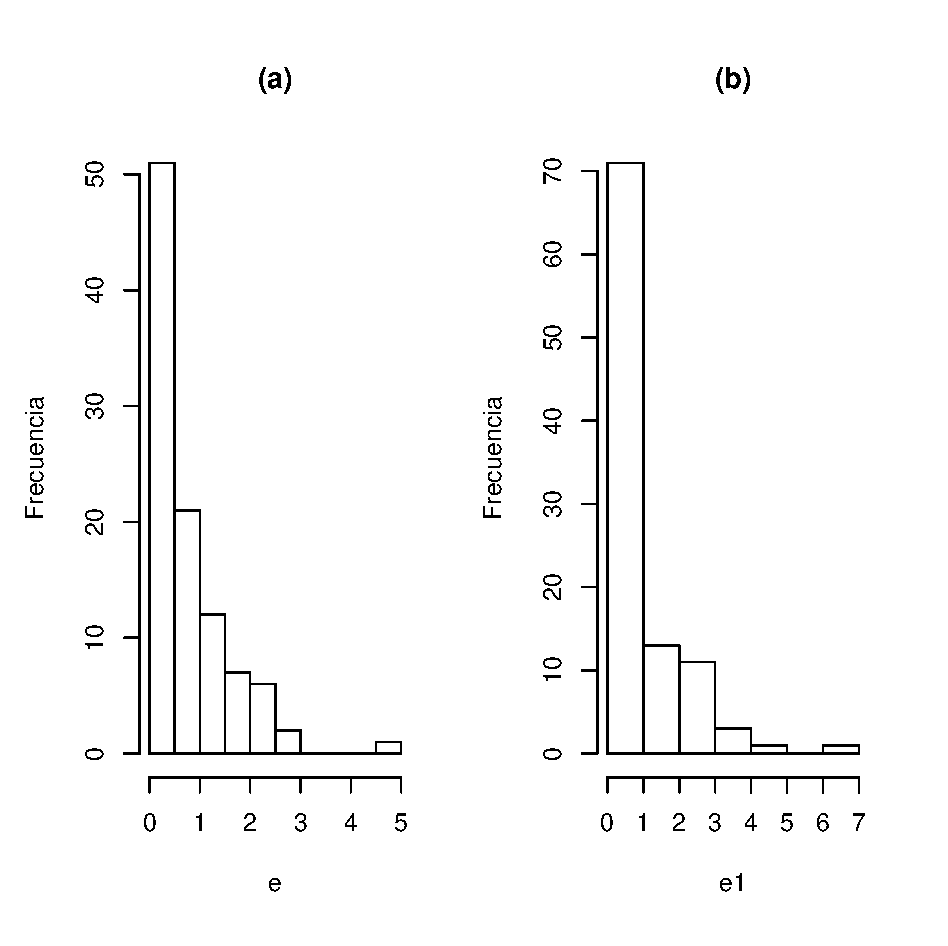
\includegraphics[scale=0.55]{exp_unif.eps}
\caption[\textsl{Histogramas de datos simulados de la distribuci�n $Exp(1)$}]{\textsl{Histogramas de 100 observaciones simulados de una distribuci�n $Exp(1)$, (a) con el Resultado 1.1.10, (b) con la instrucci�n rexp.}}
\end{figure}

Las siguientes propiedades de una distribuci�n uniforme continua se pueden comprobar f�cilmente.
\begin{Res}
Si $X$ es una variable aleatoria con distribuci�n uniforme continua sobre $[a,b]$, entonces
    \begin{enumerate}
        \item $E(X)=\frac{a+b}{2}$.
        \item $Var(X)=\frac{(b-a)^2}{12}$.
        \item $m_X(t)=\frac{e^{bt}-e^{at}}{(b-a)t}$.
    \end{enumerate}
\end{Res}

\begin{proof}
Se deja como ejercicio (Ejercicio 1.8).
\end{proof}

\subsubsection{Distribuci�n Gamma\index{Distribuci�n!Gamma}}

La distribuci�n Gamma es una distribuci�n muy importante, puesto que muchas distribuciones de uso com�n, como la distribuci�n exponencial y la distribuci�n Ji-cuadrado, son casos particulares de esta distribuci�n. La definici�n de esta distribuci�n en t�rmino de la funci�n de densidad de probabilidad est� dada por

\begin{Defi}
Una variable aleatoria $X$ tiene distribuci�n Gamma con par�metro de forma $k>0$ y par�metro de escala $\theta>0$ si su funci�n de densidad est� dada por:
\begin{equation}
f_X(x)=\frac{x^{k-1}e^{-x/\theta}}{\theta^k\Gamma(k)}I_{(0,\infty)}(x),
\end{equation}
donde $\Gamma(k)$ es la funci�n Gamma dada por
\begin{equation}
\Gamma(k)=\int_{0}^\infty u^{k-1}e^{-u}du.
\end{equation}
En este libro, se usar� la notaci�n $X\sim Gamma(k,\theta)$.
\end{Defi}

La distribuci�n Gamma tiene dos par�metros: $k$ que se denomina el par�metro de forma y $\theta$ el de escala. En este caso, el vector de par�metros es $\btheta=(k,\theta)'$ donde el espacio param�trico est� dado por $\bTheta=(0,\infty)\times(0,\infty)$. Pero cuando uno de los dos par�metros es fijo por ejemplo, si $\theta$ es fijo, entonces la distribuci�n tendr�a un solo par�metro: $k$.

\begin{figure}[!htb]
\centering
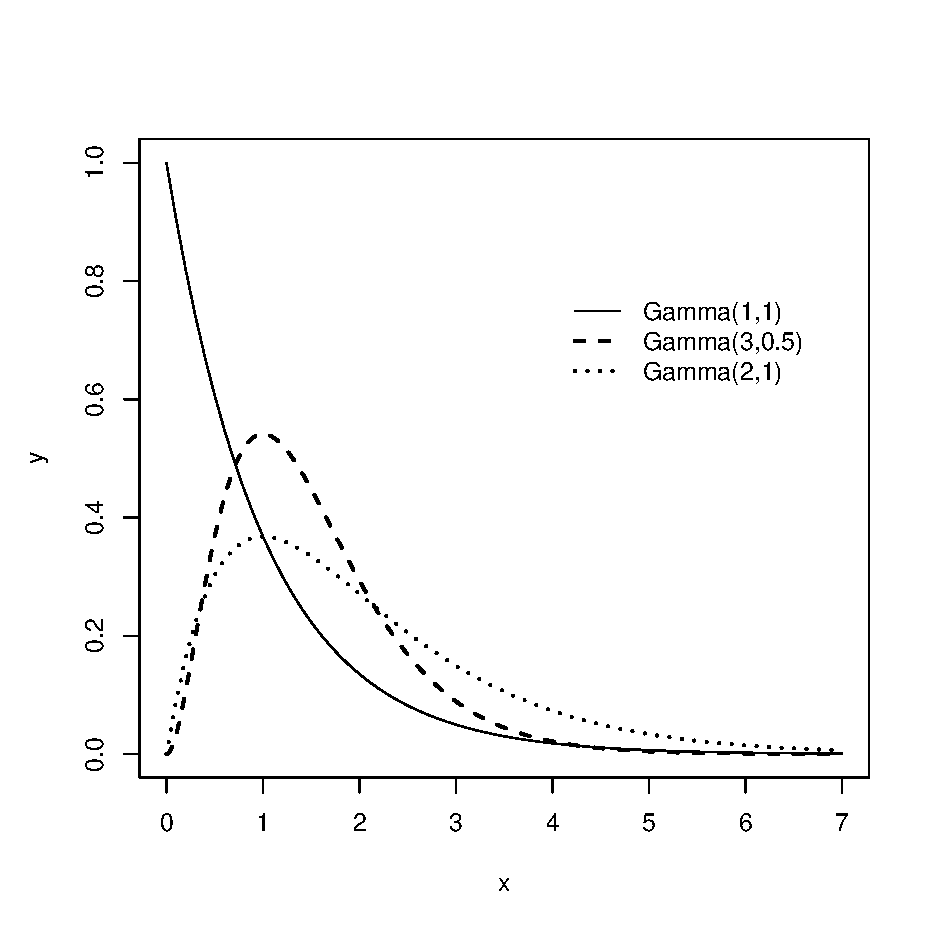
\includegraphics[scale=0.45]{distribucion_gamma.eps}
\caption{\textsl{Funciones de densidad de la distribuci�n Gamma.}}
\end{figure}

N�tese que, en primer lugar, una variable con distribuci�n s�lo puede tomar valores positivos, y en segundo lugar, la funci�n de densidad no es sim�trica puesto que el coeficiente de asimetr�a es positivo. En la Figura 1.18, se muestran algunas funciones de densidad de la distribuci�n Gamma en las cuales se observa claramente la caracter�stica no sim�trica.

Los datos del ingreso salarial cuentan con la estructura de la distribuci�n Gamma, puesto que la mayor�a de la poblaci�n tiene ingreso inferior a, por ejemplo, los 500 mil pesos colombianos, y a medida que aumenta el salario, menor n�mero de individuos puede obtener este ingreso. Observe la Figura 1.19 donde se dispone el histograma de datos que denotan el ingreso: n�tese que la clase dominante se encuentra alrededor de los 500 mil pesos, y a medida que incrementa el ingreso, menos datos se ubican en ese rango, y adem�s se presenta una cola larga hacia la derecha, las cuales son caracter�sticas propias de una distribuci�n Gamma.

\begin{figure}[!htb]
\centering
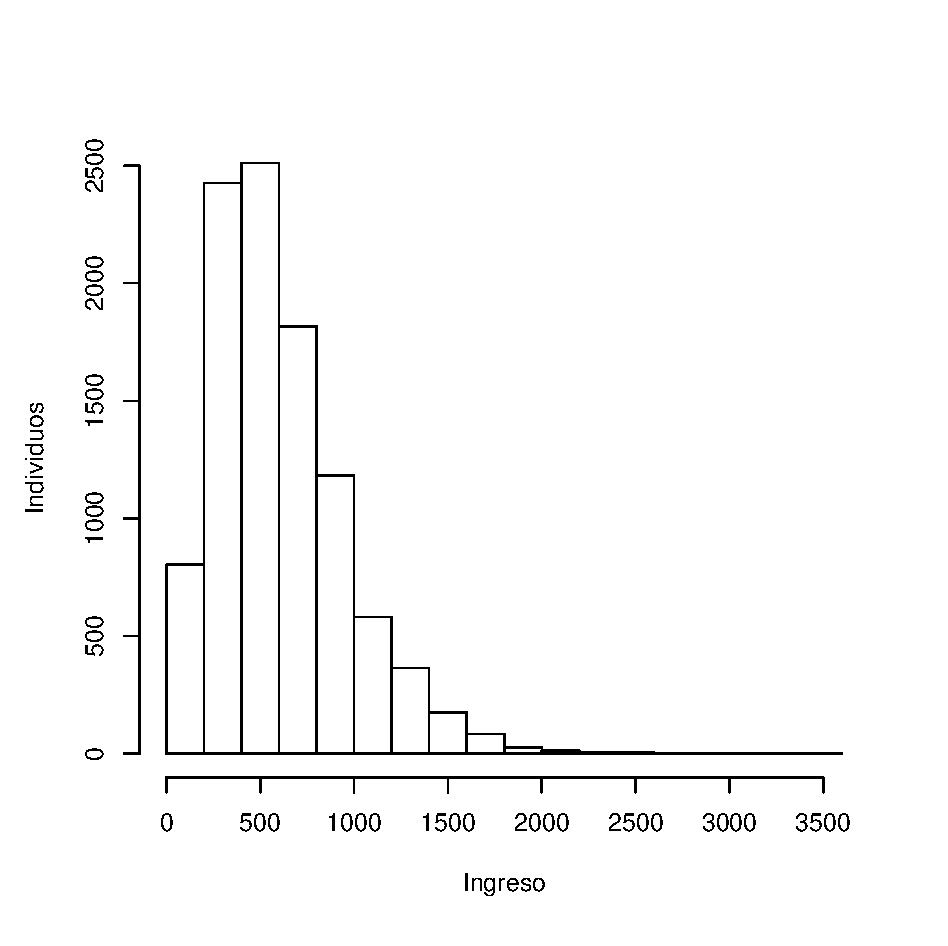
\includegraphics[scale=0.5]{hist_gamma.eps}
\caption[\textsl{Histograma de datos del tipo Gamma}]{\textsl{Histograma de un conjunto de 10 mil datos con caracter�sticas de una distribuci�n Gamma.}}
\end{figure}

Algunas propiedades de la distribuci�n Gamma se enuncian a continuaci�n.
\begin{Res}
Si $X$ es una variable aleatoria con distribuci�n Gamma con pa\-r�\-me\-tro de forma $k$ y par�metro de escala $\theta$, entonces
    \begin{enumerate}
        \item $E(X)=k\theta$.
        \item $Var(X)=k\theta^2$.
        \item $m_X(t)=\left(\frac{1}{1-\theta t}\right)^k$ para $t<1/\theta$, y no existe para otros valores de $t$.
    \end{enumerate}
\end{Res}

Del anterior resultado, podemos ver que el par�metro de escala $\theta$ se puede escribir como funci�n de la esperanza y la varianza de la distribuci�n como $\theta=Var(X)/E(X)$, y por consiguiente, se tiene que el par�metro de forma se puede escribir como $k=E(X)/\theta=(E(X))^2/Var(X)$. De esta forma, para un conjunto de datos, una vez haya identificado que siguen una distribuci�n Gamma, podemos calcular el promedio y la varianza de los datos y usarlos para tener un acercamiento a los dos par�metros de la distribuci�n como $\theta'=s^2/\bar{x}$ y $k'=\bar{x}^2/s^2$.\footnote{Este concepto se conoce como la estimaci�n de los par�metros que se discutir� en el siguiente cap�tulo.} El siguiente programa en R simula muestras de diferentes tama�os provenientes de una distribuci�n $Gamma(3,2)$, y en cada una de estas muestras calculan $\theta'$ y $k'$.

\begin{verbatim}
> set.seed(1234)
> n<-c(10,30,50,100,300,500,1000)
> tg<-matrix(NA)
> kg<-matrix(NA)
>
> for(i in 1:length(n)){
+ d<-rgamma(n[i],shape=3,scale=2)
+ tg[i]<-var(d)/mean(d)
+ kg[i]<-mean(d)/tg[i]
+ }
>
> par(mfrow=c(2,1))
> plot(tg,type="b",ylab="",xaxt="n",xlab="n",
+ main="Par�metro de escala")
> axis(1,1:length(n),n)
> abline(h=2)
>
> plot(kg,type="b",ylab="",xaxt="n",xlab="n",
+ main="Par�metro de forma")
> axis(1,1:length(n),n)
> abline(h=3)
\end{verbatim}

Como resultado del anterior programa, se tiene la Figura 1.20, donde las dos l�neas horizontales representan los valores verdaderos de $\theta$ y $k$. Podemos observar que los valores de $\theta'$ y $k'$ se encuentran aproximadamente alrededor de los valores verdaderos, pero a medida que la muestra crece, no se observa mejora alguna.

\begin{figure}[!htb]
\centering
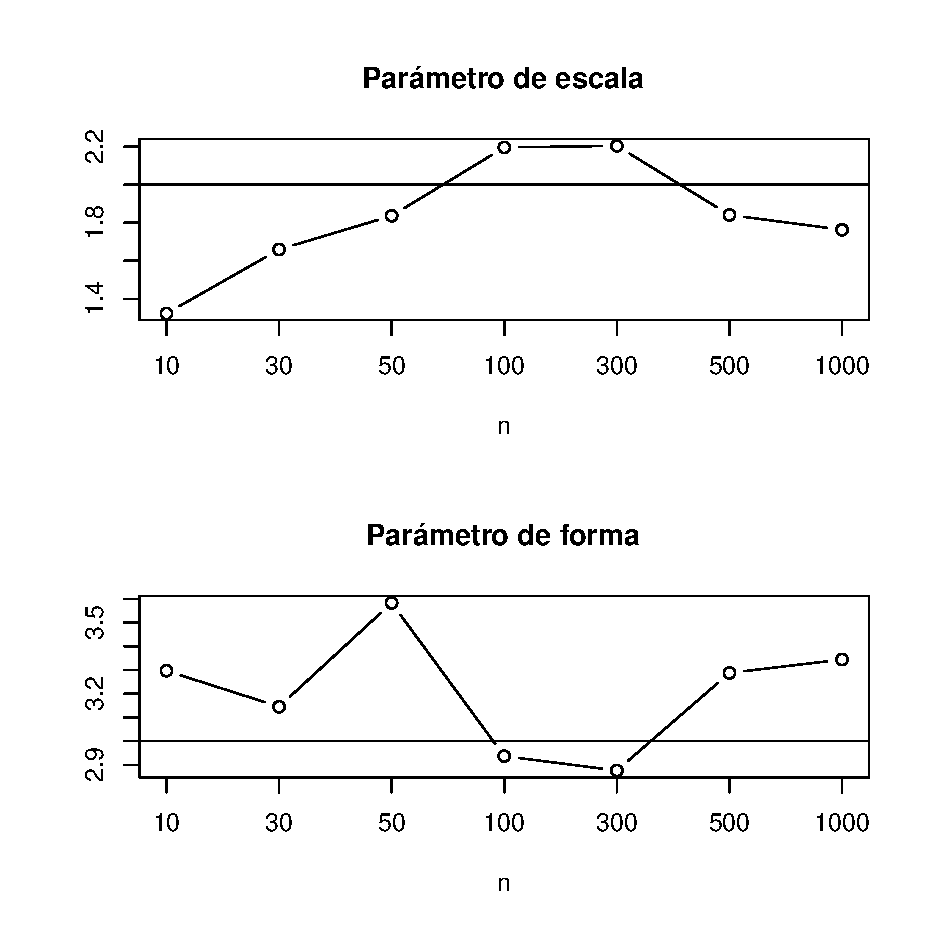
\includegraphics[scale=0.6]{est_Gamma.eps}
\caption[\textsl{Estimaci�n de $k$ y $\theta$ en una distribuci�n Gamma}]{\textsl{Estimaci�n de $k$ y $\theta$ en muestras provenientes de una distribuci�n Gamma de diferentes tama�os.}}
\end{figure}

La distribuci�n Gamma tiene una buena propiedad que establece que la suma de variables con distribuci�n Gamma puede seguir teniendo la distribuci�n Gamma bajo algunos supuestos. Esta propiedad ser� �til para algunos desarrollos en los siguiente cap�tulos, y lo enunciamos en el siguiente resultado.
\begin{Res}
Sea $X_1$, $\cdots$, $X_n$ variables aleatorias independientes con distribuci�n Gamma con par�metro de forma $k_i$ y par�metro de escala $\theta$ para $i=1,\cdots,n$, entonces la variable $\sum_{i=1}^nX_i$ tiene distribuci�n Gamma con par�metro de forma $\sum_{i=1}^nk_i$ y par�metro de escala $\theta$.
\end{Res}
\begin{proof}
An�logo a la demostraci�n del Resultado 1.1.4 y se deja como ejercicio (Ejercicio 1.9).
\end{proof}

Existe otro resultado interesante que liga la distribuci�n Gamma con la distribuci�n Poisson, y nos ser� de utilidad m�s adelante.
\begin{Res}
Si $X$ es una variable aleatoria con distribuci�n $Gamma(k,\theta)$ donde $k$ es un n�mero entero positivo, entonces para todo $x$, se tiene que $P(X\leq x)=P(Y\geq k)$ donde $Y$ es una variable aleatoria con distribuci�n $Pois(x/\theta)$.
\end{Res}

Podemos verificar de forma num�rica la validez del anterior resultado. Sea $X\sim Gamma(2,3.5)$, y $x=4.2$ entonces $Pr(X\leq x)=Pr(X\leq 4.2)$ y se puede calcular con el comando \verb"pgamma(4.2,shape=2,scale=3.5)" y arroja como resultado 0.337. Por otro lado, de acuerdo al resultado anterior, $Y\sim Pois(4.2/3.5)=Pois(1.2)$ y $Pr(Y\geq k)=Pr(Y\geq 2)$, el cual se calcula con el comando \verb"ppois(k,4.2/3.5,lower" \verb".tail=F)+dpois(k,4.2/3.5)", y arroja el mismo resultado 0.337.

De lo anterior observamos que una probabilidad con respecto a una variable con distribuci�n Gamma se puede calcular en t�rminos de una variable Poisson; el rec�proco tambi�n es cierto. Suponga que $Y\sim Pois(5.3)$, entonces $Pr(Y\geq4)$ se puede calcular con \verb"ppois(4,5.3,lower.tail=F)+dpois(4,5.3)" y da como resultado 0.774. Pero de acuerdo al anterior resultado, esta probabilidad tambi�n se puede calcular como $Pr(X\leq x)$ donde $X$ tiene distribuci�n Gamma como par�metro de escala $k=4$, y el par�metro de escala $\theta$ debe satisfacer $x/\theta=5.3$, y de esta ecuaci�n se pueden hallar infinitas soluciones para $x$ y $\theta$; por ejemplo, al tomar $x=1$, tenemos que $\theta=1/5.3$, y as� tenemos $Pr(X\leq 1)$ con $X\sim Gamma(4,1/5.3)$. Al calcular esta probabilidad con \verb"pgamma(1,shape=4,scale=1/5.3)" tenemos la misma probabilidad 0.774. El lector puede comprobar que si se hubiera escogido otro valor para $x$, por ejemplo $x=10$, y se halla el valor $\theta=x/5.3$, la probabilidad de $Pr(X\leq 10)$ tambi�n es 0.774.

Con lo anterior, vemos que la probabilidad concerniente a una distribuci�n Poisson puede ser calculada en t�rminos de infinitas distribuciones Gamma. En particular si escogemos $\theta=2$, la distribuci�n Gamma se reduce a una distribuci�n $\chi^2$, y tenemos el siguiente resultado que es una consecuencia inmediata del Resultado 1.1.14.
\begin{Res}
Si $Y$ es una variable aleatoria con distribuci�n $Pois(\lambda)$, entonces para cualesquieras enteros $y_1$ y $y_2$, se tiene que
\begin{equation*}
P(Y\geq y_1)=P(X\leq2\lambda)
\end{equation*}

donde $X\sim\chi^2_{2y_1}$. Y
\begin{equation*}
P(Y\leq y_2)=1-P(Y\geq y_2+1)=1-P(X\leq2\lambda)
\end{equation*}
donde $X\sim\chi^2_{2(y_2+1)}$.
\end{Res}

\subsubsection{Distribuci�n exponencial\index{Distribuci�n!exponencial}}

La distribuci�n exponencial es un caso particular de la distribuci�n Gamma cuando el par�metro de forma $k$ toma el valor 1,  y por consiguiente se puede obtener f�cilmente la funci�n de densidad dada a continuaci�n.
\begin{Defi}
Una variable aleatoria $X$ tiene distribuci�n exponencial con par�metro de escala $\theta>0$ si su funci�n de densidad est� dada por:
\begin{equation}\label{densidad_exp}
f_X(x)=\frac{1}{\theta}e^{-x/\theta}I_{(0,\infty)}(x),
\end{equation}
y en este libro, se usar� la notaci�n $X\sim Exp(\theta)$.
\end{Defi}

Una variable exponencial toma valores en el intervalo $(0,\infty)$, y puede ser utilizada para describir el tiempo necesario para la ocurrencia de alg�n evento o la vida �til de un componente el�ctrico. En la Figura 1.21 se muestra la funci�n de densidad de la distribuci�n exponencial con diferentes valores de $\theta$. En primer lugar, se observa que la funci�n de densidad es siempre decreciente, y por consiguiente, para una variable $X\sim Exp(\theta)$, se tiene que $Pr(t_1<X<t_1+\delta)<Pr(t_2<X<t_2+\delta)$ si $t_1>t_2$. Para ver la interpretaci�n de eso, suponga que $X$ denota la vida �til (en a�os) de una referencia de lavadora, entonces, como es natural, se afirma que es m�s probable que la lavadora funcione entre 2 y 3 a�os que entre 6 y 7 a�os, esto es, $Pr(6<X<7)<Pr(2<X<3)$, que es una caracter�stica reflejada en la funci�n de densidad de una distribuci�n exponencial.

M�s a�n, suponga que dos tipos de lavadoras, A y B, tienen la vida �til (en a�os) que puede ser descrita por la distribuci�n $Exp(2)$ y $Exp(5)$, respectivamente. Entonces, por el Resultado 1.1.12, donde provee propiedades de una distribuci�n Gamma, podemos afirmar que las vidas �tiles promedio de A y B son 2 y 5 respectivamente, es decir, las lavadoras del tipo B pueden funcionar por m�s a�os que los del tipo A. Por tanto, intuitivamente podemos afirmar que la probabilidad de que una lavadora funcione m�s de 6 a�os debe ser mayor en las del tipo B que en el tipo A, y recordando que esta probabilidad corresponde al �rea bajo la funci�n de densidad en el intervalo $(6,\infty)$, podemos observar que la anterior afirmaci�n s� se refleja en la Figura 1.21. Dadas las anteriores observaciones, podemos ver por qu� la distribuci�n exponencial es usada para describir este tipo de variables.

\begin{figure}[!htb]
\centering
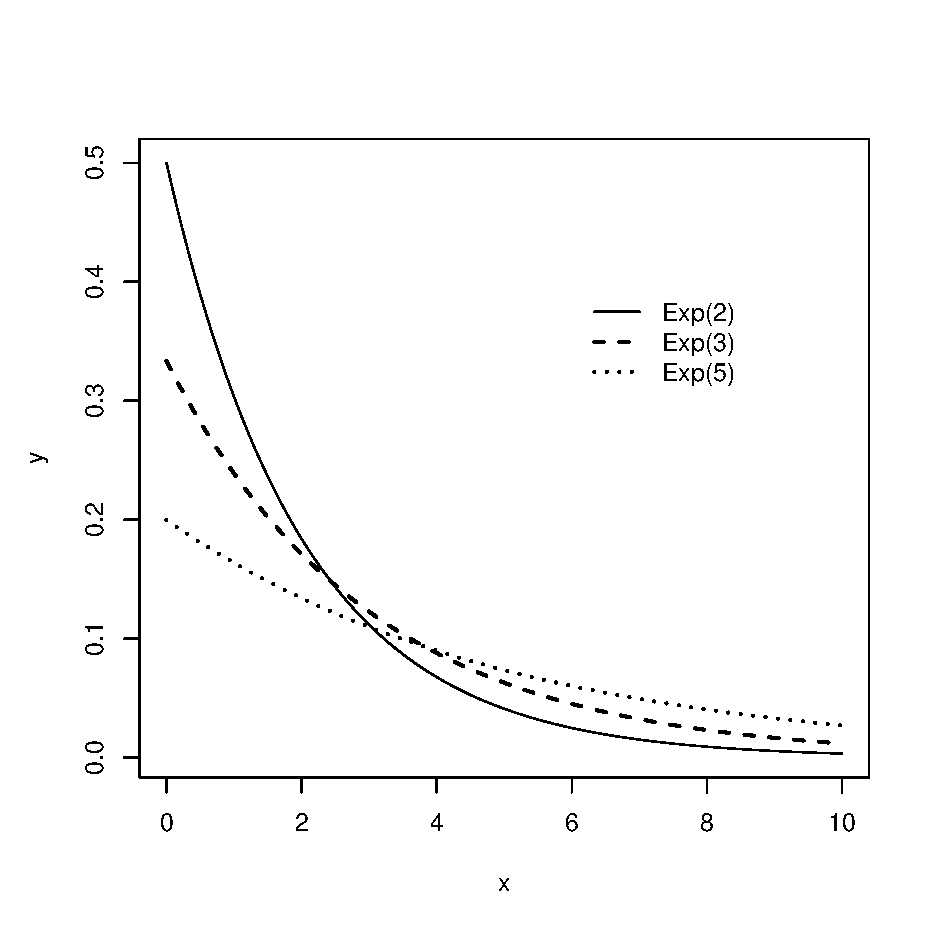
\includegraphics[scale=0.5]{densidad_exponencial.eps}
\caption{\textsl{Funci�n de densidad de distribuciones $Exp(2)$, $Exp(3)$ y $Exp(5)$.}}
\end{figure}

Ahora bien aunque muchas veces se ha dicho en la literatura estad�stica que una variable aleatoria que denota el tiempo puede ser descrita por la distribuci�n exponencial dado que �sta siempre toma valores positivos, caracter�stica propia de la variable tiempo, la funci�n de densidad de la distribuci�n exponencial es siempre decreciente, y puede no ser apta para algunas situaciones; por ejemplo, considere una central telef�nica que atiende quejas de consumidores. Si se desea estudiar la variable $X$ definida como el tiempo de duraci�n de una llamada hecha por un consumidor, no es natural pensar que la probabilidad de que la llamada dura menos de un minuto sea mayor a la probabilidad de que dura menos de 5 minutos, esto es, puede no suceder que $Pr(X<1)>Pr(X<5)$; en otras palabras, no necesariamente, entre m�s corta sea la llamada, mayor probabilidad tiene asociada. Y en este caso, la distribuci�n exponencial no resulta adecuada, sino posiblemente una distribuci�n Gamma. N�tese que la distribuci�n exponencial es un caso particular de la distribuci�n Gamma, por consiguiente se pueden obtener f�cilmente sus propiedades usando el Resultado 1.1.12.

\begin{Res}
Si $X$ es una variable aleatoria con distribuci�n exponencial con par�metro $\theta$, entonces
    \begin{enumerate}
        \item $E(X)=\theta$.
        \item $Var(X)=\theta^2$.
        \item $m_X(t)=\frac{1}{1-\theta t}$ para $t<1/\theta$, y no existe para otros valores de $t$.
    \end{enumerate}
\end{Res}

N�tese que la varianza te�rica de la distribuci�n es el cuadrado de la esperanza. De esta forma, si un conjunto de datos continuos positivo tiene la varianza aproximadamente igual al promedio al cuadrado, podr�amos afirmar que los datos provienen de una distribuci�n exponencial.


El siguiente resultado es un caso particular del Resultado 1.1.13 y ser� de utilidad en los siguientes cap�tulos.
\begin{Res}
Sea $X_1$, $\cdots$, $X_n$ variables aleatorias independientes e id�nticamente distribuidas con distribuci�n exponencial con par�metro de escala $\theta$, entonces la variable $\sum_{i=1}^nX_i$ tiene distribuci�n Gamma con par�metro de forma $n$ y par�metro de escala $\theta$.
\end{Res}

\subsubsection{Distribuci�n Weibull\index{Distribuci�n!Weibull}}

La distribuci�n Weibull debe su nombre al sueco Ernst Hjalmar Waloddi Weibull (1887-1979) y es �til en la rama de la estad�stica denominada an�lisis de sobrevivencia donde se estudian variables que denotan el tiempo transcurrido hasta que suceda un evento como fallecimiento de un paciente o falla de alg�n componente el�ctrico.

\begin{figure}[!htb]
\centering
\includegraphics[bb=0 0 472 738, scale=0.2]{Mr_Weibull.jpg}
\caption{\textsl{Ernst Hjalmar Waloddi Weibull (1887-1979).}}
\end{figure}

\newpage

La funci�n de densidad de esta distribuci�n se da a continuaci�n.

\begin{Defi}
Una variable $X$ tiene distribuci�n Weibull con par�metro de forma $k>0$ y par�metro de escala $\theta>0$ si la funci�n de densidad de $X$ est� dada por
\begin{equation}\label{densidad_weibull}
f_X(x)=\frac{k}{\theta^k}x^{k-1}\exp\left\{-\frac{x^k}{\theta^k}\right\}I_{(0,\infty)}(x).
\end{equation}

Denotaremos esta distribuci�n con $X\sim Weibull(k,\theta)$.
\end{Defi}

N�tese que la funci�n de densidad de una distribuci�n Weibull es similar en algunos t�rminos a la de la distribuci�n Gamma. De hecho, cuando el par�metro $k$ toma valor 1, la distribuci�n Weibull se reduce a una distribuci�n Exponencial de media $\theta$. En la Figura 1.23 se muestran algunas funciones de densidad de la distribuci�n Weibull con diferentes valores de $k$ y $\theta$. Podemos observar que la funci�n de densidad de la distribuci�n Weibull(1,1) tiene la misma funci�n de densidad que una distribuci�n exponencial.

\begin{figure}[!htb]
\centering
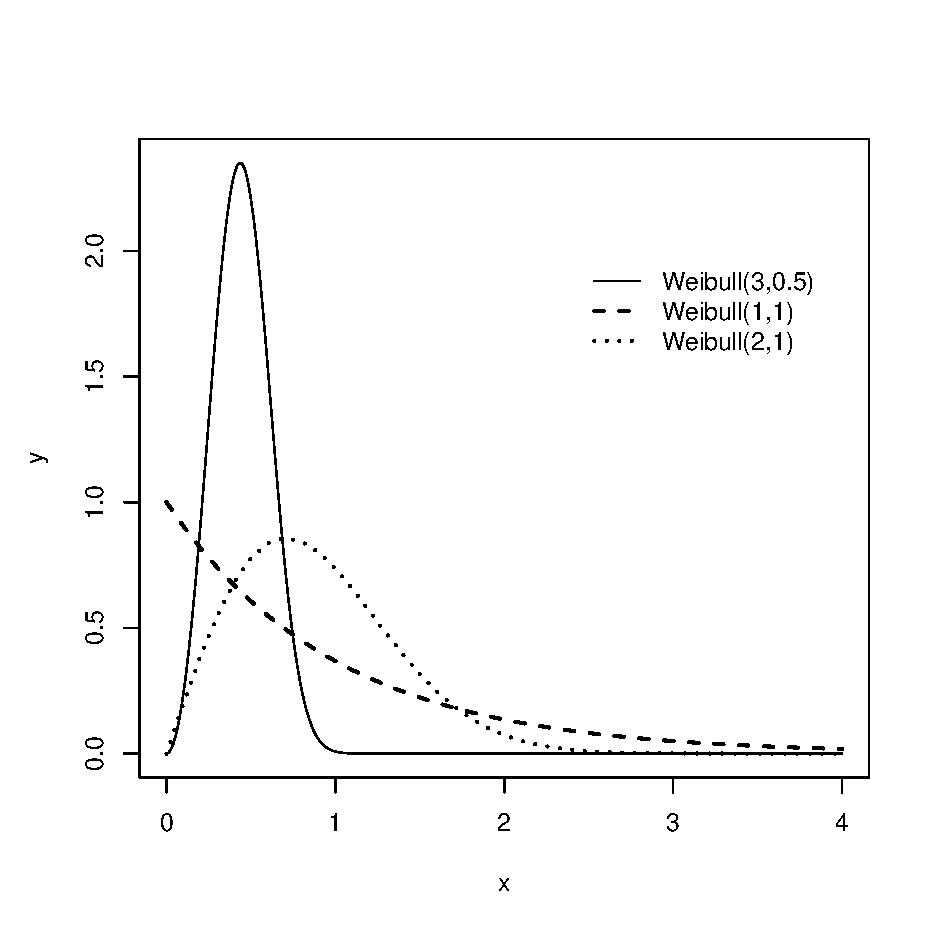
\includegraphics[scale=0.6]{densidad_Weibull.eps}
\caption[\textsl{Densidad de una distribuci�n Weibull}]{\textsl{Funci�n de densidad de una distribuci�n Weibull con diferentes pa\-r�\-me\-tros.}}
\end{figure}

Algunas propiedades de la distribuci�n Weibull se dan a continuaci�n.

\begin{Res}
Si $X$ es una variable aleatoria con distribuci�n $Weibull(k,\theta)$, entonces
\begin{enumerate}
  \item $E(X)=\theta\Gamma\left(1+\frac{1}{k}\right)$,
  \item $Var(X)=\theta^2\left[\Gamma\left(1+\frac{2}{k}\right)-\left(\Gamma\left(1+\frac{1}{k}\right)\right)^2\right]$
\end{enumerate}
\end{Res}


\subsubsection{Distribuci�n normal\index{Distribuci�n!normal}}

La distribuci�n normal tambi�n es llamada la distribuci�n gaussiana, rindiendo ho\-me\-na\-je al matem�tico alem�n Carl Friedrich Gauss (1777-1855). Esta distribuci�n es, sin duda, una de las distribuciones m�s importantes, y de uso m�s frecuente en la teor�a estad�stica, puesto que una gran parte de la teor�a estad�stica fue desarrollada inicialmente para variables con esta distribuci�n. Por otra parte, gracias al teorema del l�mite central, muchas distribuciones ajenas a la normal, incluyendo las variables discretas, pueden ser aproximadas por �sta cuando el tama�o muestral es grande. Para detalles sobre la historia de la distribuci�n normal, consulte a \citeasnoun{normal}.

\begin{figure}[!htb]
\centering
\includegraphics[bb=0 0 468 600, scale=0.3]{Gauss.jpg}
\caption{\textsl{Carl Friedrich Gauss (1777-1855).}}
\end{figure}

\begin{Defi}
Una variable aleatoria $X$ tiene distribuci�n normal con par�metros $\mu$ y $\sigma^2$ si su funci�n de densidad est� dada por:
\begin{equation}
f_X(x)=\frac{1}{\sqrt{2\pi\sigma^2}}\exp\left\{-\frac{1}{2\sigma^2}(x-\mu)^2\right\}I_\mathbb{R}(x),
\end{equation}
donde $\sigma>0$ y se nota como $X\sim N(\mu,\sigma^2)$.
\end{Defi}
La distribuci�n normal tiene dos par�metros, representado como $\btheta=(\mu,\sigma^2)$ y $\bTheta=\mathbb{R}\times(0,\infty)$. Cada uno de los dos par�metros de la distribuci�n normal determina un aspecto espec�fico de la distribuci�n. En primer lugar, se puede ver f�cilmente que para cualquier valor $x$, se tiene que $f(\mu+x)=f(\mu-x)$, de donde se deduce que la funci�n de densidad es sim�trica con respecto a $\mu$. En segundo lugar, la funci�n de densidad toma el valor m�ximo en el punto $x=\mu$, y el m�ximo es igual a $(2\pi\sigma^2)^{-1/2}$, de donde se tiene que entre m�s peque�o sea el valor de $\sigma^2$, el �rea bajo la funci�n de densidad est� m�s concentrada alrededor del valor $\mu$. En la Figura 1.25, se muestran algunas funciones de densidad para diferentes valores de $\mu$ y $\sigma^2$, donde se puede confirmar lo comentado anteriormente.

\begin{figure}[!htb]
\centering
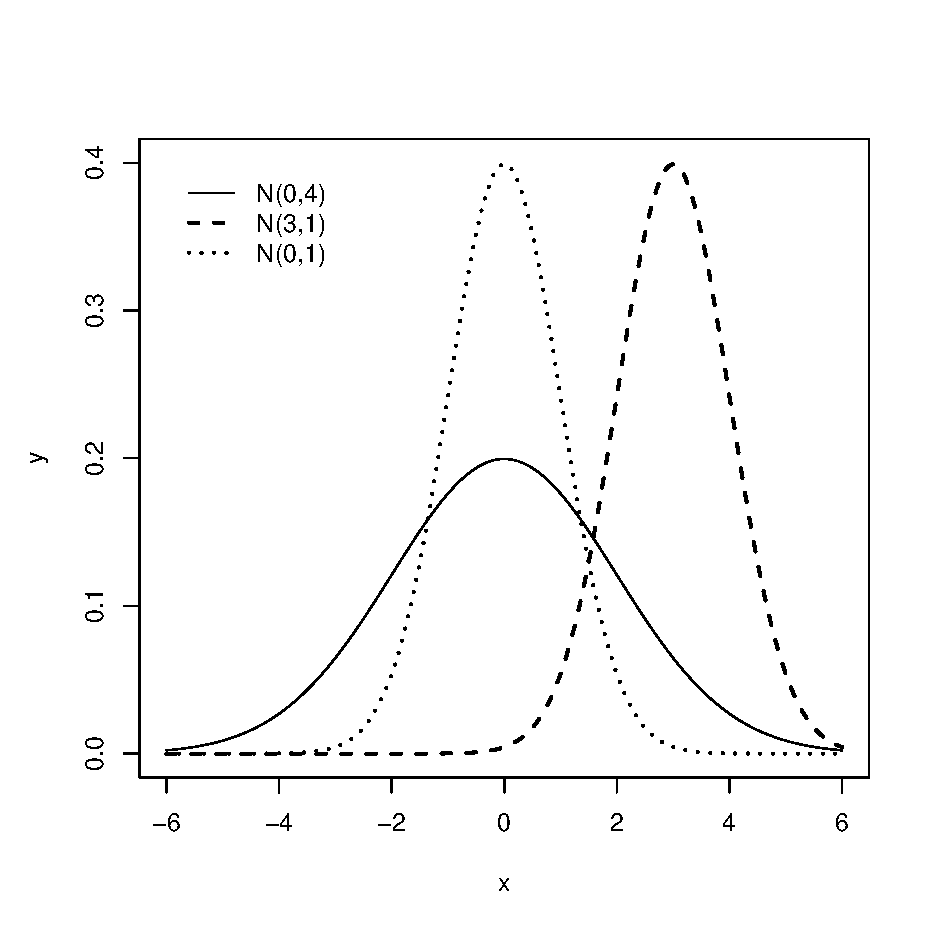
\includegraphics[scale=0.6]{densidad_normal.eps}
\caption[\textsl{Densidad de una distribuci�n normal}]{\textsl{Funci�n de densidad de una distribuci�n normal con diferentes par�metros.}}
\end{figure}

Ahora, haciendo una analog�a entre el histograma de un conjunto de datos y una funci�n de densidad, podemos sospechar que en primer lugar, si los datos provienen de una distribuci�n normal, entonces el valor $\mu$ debe ubicarse alrededor del punto centro de los datos; y en segundo lugar, el valor $\sigma^2$ est� asociado con la variaci�n de los datos, ya que entre m�s peque�a sea �sta, m�s concentrados estar�n los datos. El siguiente resultado confirma esta sospecha.

\begin{Res}
Si $X$ es una variable aleatoria con distribuci�n normal con pa\-r�\-me\-tros $\mu$ y $\sigma^2$, entonces
    \begin{enumerate}
        \item $E(X)=\mu$.
        \item $Var(X)=\sigma^2$.
        \item $m_X(t)=\exp\left\{\mu t+\frac{1}{2}\sigma^2t^2\right\}$.
    \end{enumerate}
\end{Res}

En la vida pr�ctica, para que un conjunto de datos tenga distribuci�n normal, una herramienta b�sica es examinar si el histograma de los datos tiene la forma llamada campana de Gauss, esto es, caracter�sticas similares a la funci�n de densidad presentada en la Figura 1.25. La mayor frecuencia debe estar asociada con la clase media, y a medida que las clases se alejan de la clase media, la frecuencia debe disminuir sim�tricamente. En la Figura 1.26 se muestra el histograma de varios conjuntos de datos simulados usando la funci�n \verb"rnorm" de R. Obs�rvese que la caracter�stica de la distribuci�n normal es muy preeminente en muestras grandes, mientras que en muestras peque�as, la detecci�n de la normalidad mediante el histograma puede ser inadecuada.

\begin{figure}[!htb]
\centering
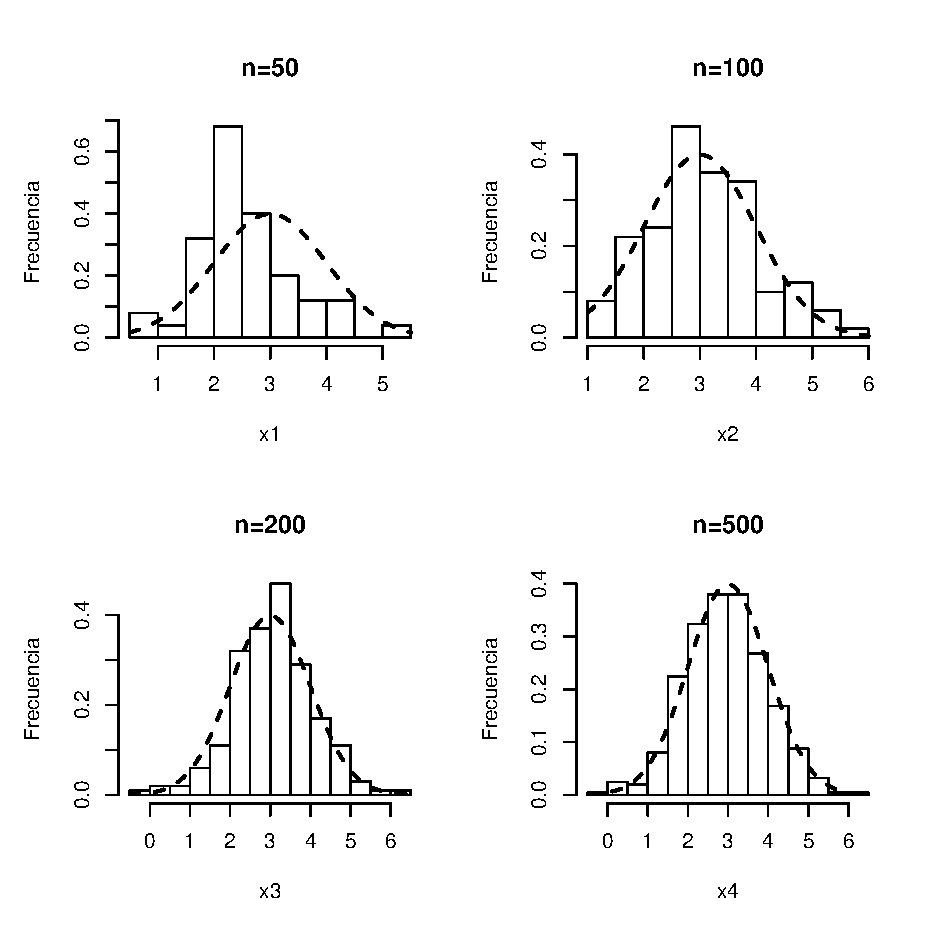
\includegraphics[scale=0.6]{hist_normal.eps}
\caption[\textsl{Histograma de datos provenientes de una distribuci�n normal}]{\textsl{Histograma de grupos de datos provenientes de la distribuci�n normal con diferentes tama�os muestrales.}}
\end{figure}

Una propiedad muy particular de la distribuci�n normal es que la distribuci�n se conserva para transformaciones lineales, y se enuncia a continuaci�n.

\begin{Res}
Si $X\sim N(\mu,\sigma^2)$, y $\alpha$, $\beta$ son constantes, entonces la variable $\alpha X+\beta$ tiene distribuci�n $N(\alpha\mu+\beta,\alpha^2\sigma^2)$.
\end{Res}
\begin{proof} Se usar� el hecho de que la funci�n generadora de momentos ca\-ra\-cte\-riza la distribuci�n probabil�stica. Se tiene que:
\newpage
\begin{align*}
m_{\alpha X+\beta}(t)&=E(e^{t(\alpha X+\beta)})\\
                     &=E(e^{\alpha tX})e^{\beta t}\\
                     &=m_X(\alpha t)e^{\beta t}\\
                     &=e^{\mu\alpha t+\sigma^2\alpha^2t/2}e^{\beta t}\\
                     &=e^{(\alpha\mu+\beta)t+\sigma^2\alpha^2t/2}
\end{align*}
la cual es la funci�n generadora de momentos de una distribuci�n $N(\alpha\mu+\beta,\alpha^2\sigma^2)$, y el resultado queda demostrado.
\end{proof}

Como consecuencia inmediata del anterior resultado, se define la estandarizaci�n que es fundamental en la teor�a relacionada con las distribuciones normales.

\begin{Defi}
Si $X\sim N(\mu,\sigma^2)$ con $\mu=0$ y $\sigma=1$, entonces se dice que $X$ tiene distribuci�n normal est�ndar\index{Distribuci�n!normal est�ndar} y usualmente se denota por $Z$.
\end{Defi}

Utilizando el Resultado 1.1.20, podemos comprobar que una variable $X\sim N(\mu,\sigma^2)$ puede ser transformada a una variable $Z$ mediante una transformaci�n lineal. Suponga que esta transformaci�n se denota por $\alpha X+\beta$, entonces encontrar los valores de $\alpha$ y $\beta$ para los cuales la variable transformada tenga distribuci�n normal est�ndar equivale a solucionar las siguientes igualdades para $\alpha$ y $\beta$

\begin{equation*}
\begin{cases}
\alpha\mu+\beta=0\\
\alpha^2\sigma^2=1
\end{cases}
\end{equation*}

de donde se tienen dos soluciones $\alpha_1=1/\sigma$, $\beta_1=-\mu/\sigma$ y $\alpha_2=-1/\sigma$, $\beta_2=\mu/\sigma$. Y de esta forma, hemos encontrado dos variables $Z_1=\frac{X-\mu}{\sigma}$ y $Z_2=\frac{\mu-X}{\sigma}$ con la distribuci�n normal est�ndar. Sin embargo, se acostumbra a utilizar la transformaci�n dada por la primera soluci�n, y esta transformaci�n se conoce como la estandarizaci�n, y la variable $Z=Z_1=\frac{X-\mu}{\sigma}$ se conoce como la variable $X$ estandarizada.

An�loga a las distribuciones Poisson, Gamma, la distribuci�n normal tambi�n se conserva para suma de variables normales independientes, tal como lo muestra el siguiente resultado.

\begin{Res}
Sea $X_1$, $\cdots$, $X_n$ variables aleatorias independientes, donde $X_i\sim N(\mu_i,\sigma^2_i)$ con $i=1,\cdots,n$, entonces la variable $\sum_{i=1}^nX_i\sim N(\sum_{i=1}^n\mu_i,\sum_{i=1}^n\sigma_i^2)$.
\end{Res}
\begin{proof}
Se deja como ejercicio (Ejercicio 1.13).
\end{proof}

Combinando los resultados 1.1.20 y 1.1.21, se puede establecer que el promedio de variables independientes con la misma distribuci�n normal sigue teniendo distribuci�n normal, y lo enunciamos a continuaci�n.

\begin{Res}
Sea $X_1$, $\cdots$, $X_n$ variables aleatorias independientes e id�nticamente distribuidas con distribuci�n $N(\mu,\sigma^2)$, entonces la variable $\bar{X}=\sum_{i=1}^nX_i/n$ tiene distribuci�n $N(\mu,\sigma^2/n)$.
\end{Res}

\begin{proof}
Se deja como ejercicio (Ejercicio 1.14).
\end{proof}

Una de las razones por las que la distribuci�n normal es de las m�s importantes en la teor�a estad�stica radica en el hecho de que en un conjunto de variables independientes e id�nticamente distribuidas no necesariamente con distribuci�n normal, si el n�mero de variables es grande, entonces la distribuci�n del promedio de estas variables puede ser aproximada por la de una distribuci�n normal. Lo anterior se conoce como el famoso <<teorema del l�mite Central>>\index{Teorema!del l�mite central} y se enuncia a continuaci�n.

\begin{Res}
Sea $X_1$, $X_2$, $\cdots$, una sucesi�n de variables aleatorias in\-de\-pen\-dien\-tes e id�nticamente distribuidas, suponga que las funciones generadoras de momentos $m_{X_i}(t)$ existen en una vecindad de 0, y la esperanza com�n se denota por $\mu$ y va\-rian\-za com�n se denota por $\sigma^2>0$, y se define $\bar{X}_{n}$ como $\sum_{i=1}^nX_i/n$, y la funci�n de distribuci�n de la variable $\sqrt{n}(\bar{X}_n-\mu)/\sigma$ se denota por $F_n(x)$, entonces se tiene que
\begin{equation*}
\lim_{n\rightarrow\infty}F_n(x)=\int_{-\infty}^x\dfrac{1}{\sqrt{2\pi}}e^{-y^2/2}dy,
\end{equation*}
es decir, la distribuci�n l�mite de $\sqrt{n}(\bar{X}_n-\mu)/\sigma$ corresponde a la distribuci�n normal est�ndar.
\end{Res}

\begin{proof}
Se probar� que la funci�n generadora de momentos de la variable $\sqrt{n}(\bar{X}_n-\mu)/\sigma$ converge a la funci�n $e^{t^2/2}$ que corresponde a la funci�n generadora de momentos de una distribuci�n $N(0,1)$. Para eso primero se define $Z_i$ como la variable $X_i$ estandarizada, entonces $Z_i\sim N(0,1)$ para todo $i=1,2,\cdots$. Y podemos comprobar f�cilmente que $\sqrt{n}(\bar{X}_n-\mu)/\sigma=\sum_{i=1}^nZ_i/\sqrt{n}$, entonces tenemos
\begin{align*}
m_{\sqrt{n}(\bar{X}_n-\mu)/\sigma}(t)&=m_{\sum_{i=1}^nZ_i/\sqrt{n}}(t)\\
&=\prod_{i=1}^nm_{Z_i}\left(\frac{t}{\sqrt{n}}\right)\ \ \ \ \ \ \text{por la independencia}\\
&=\left(m_Z\left(\frac{t}{\sqrt{n}}\right)\right)^n,
\end{align*}
donde $Z$ denota una variable con distribuci�n normal est�ndar. Ahora, usamos la expansi�n de Taylor para la funci�n $m_Z\left(\frac{t}{\sqrt{n}}\right)$ alrededor del punto 0. Para eso recordamos que si $g(x)$ es una funci�n derivable de cualquier orden, entonces se puede expandir $g(x)$ alrededor de un punto $a$ como
\begin{equation}\label{Taylor_g}
g(x)=\sum_{i=0}^\infty\frac{g^{(i)}(a)(x-a)^i}{i!},
\end{equation}
donde $g^{(i)}(a)$ es la $i$-�sima derivada de $g(x)$ evaluada en $x=a$ y $g^{(0)}(a)=g(a)$.

De esta forma, tenemos que
\begin{align*}
m_Z\left(\frac{t}{\sqrt{n}}\right)&=\sum_{i=0}^\infty \frac{m_Z^{(i)}(0)\left(\frac{t}{\sqrt{n}}\right)^i}{i!}\\
&=m_Z(0)+m_Z'(0)\left(\frac{t}{\sqrt{n}}\right)+\frac{1}{2}m_Z''(0)\left(\frac{t}{\sqrt{n}}\right)^2+\sum_{i=3}^\infty \frac{m_Z^{(i)}(0)\left(\frac{t}{\sqrt{n}}\right)^i}{i!}\\
&=1+\frac{1}{2}\left(\frac{t}{\sqrt{n}}\right)^2+R\left(\frac{t}{\sqrt{n}}\right),
\end{align*}
donde
\begin{equation*}
R\left(\frac{t}{\sqrt{n}}\right)=\sum_{i=3}^\infty \frac{m_Z^{(i)}(0)\left(\frac{t}{\sqrt{n}}\right)^i}{i!}.
\end{equation*}
Y por consiguiente, tenemos que
\begin{align}\label{Taylor_lim}
\lim_{n\rightarrow\infty}m_{\sqrt{n}(\bar{X}_n-\mu)/\sigma}(t)&=\lim_{n\rightarrow\infty}\left(m_Z\left(\frac{t}{\sqrt{n}}\right)\right)^n\notag\\
&=\lim_{n\rightarrow\infty}\left(1+\frac{1}{2}\left(\frac{t}{\sqrt{n}}\right)^2+R\left(\frac{t}{\sqrt{n}}\right)\right)^n\notag\\
&=\lim_{n\rightarrow\infty}\left[1+\frac{1}{n}\left(\frac{t^2}{2}+nR\left(\frac{t}{\sqrt{n}}\right)\right)\right]^n.
\end{align}

Por otro lado, el teorema de Taylor afirma que para la funci�n $g$ en (\ref{Taylor_g}), se tiene que
\begin{equation*}
\lim_{x\rightarrow a}\frac{\sum_{i=r+1}^{\infty}\frac{g^{(i)}(a)(x-a)^i}{i!}}{(x-a)^r}=0.
\end{equation*}
Aplicando lo anterior a $m_Z\left(\frac{t}{\sqrt{n}}\right)$ con $r=2$, tenemos que
\begin{equation*}
\lim_{\frac{t}{\sqrt{n}}\rightarrow0}\frac{R\left(\frac{t}{\sqrt{n}}\right)}{\left(\frac{t}{\sqrt{n}}\right)^2}=0,
\end{equation*}
la cual es equivalente a
\begin{equation*}
\lim_{n\rightarrow\infty}\frac{R\left(\frac{t}{\sqrt{n}}\right)}{\left(\frac{1}{\sqrt{n}}\right)^2}=\lim_{n\rightarrow\infty}nR\left(\frac{t}{\sqrt{n}}\right)=0,
\end{equation*}
para todo $t$. Y por consiguiente
\begin{equation}\label{Taylor_exp}
\lim_{n\rightarrow\infty}\left(\frac{t^2}{2}+nR\left(\frac{t}{\sqrt{n}}\right)\right)=\frac{t^2}{2}.
\end{equation}
Finalmente, combinando (\ref{Taylor_lim}) y (\ref{Taylor_exp}), y usando el hecho de que si una sucesi�n de n�meros $a_n\rightarrow a$, entonces $\lim_{n\rightarrow\infty}\left(1+\frac{a_n}{n}\right)^n=e^a$, se tiene que
\begin{equation*}
\lim_{n\rightarrow\infty}\left[1+\frac{1}{n}\left(\frac{t^2}{2}+nR\left(\frac{t}{\sqrt{n}}\right)\right)\right]^n=e^{t^2/2},
\end{equation*}
y en conclusi�n
\begin{equation*}
\lim_{n\rightarrow\infty}m_{\sqrt{n}(\bar{X}_n-\mu)/\sigma}(t)=e^{t^2/2}.
\end{equation*}
En conclusi�n, la distribuci�n l�mite de $\sqrt{n}(\bar{X}_n-\mu)/\sigma$ corresponde a la distribuci�n normal est�ndar.
\end{proof}

En el anterior teorema se exige la existencia de la funci�n generadora de momentos de las variables $X_1$, $X_2$, $\cdots$; en general, se puede demostrar la validez del resultado a�n sin este supuesto, y la demostraci�n se realiza por medio de funciones caracter�sticas de manera an�loga.

El teorema del l�mite central es una herramienta muy poderosa en el sentido de que se aplica para la mayor�a de las distribuciones de probabilidad; sin embargo, el teorema no nos brinda una medida de qu� tan buena es la aproximaci�n, y se debe examinar para cada distribuci�n. En las figuras 1.27 y 1.28, se muestran las distribuciones muestrales del promedio en muestras simuladas distribuciones $Pois(3)$ y $Gamma(3,2)$ con tama�os de muestral 5, 10, 30, 50, 100 y 500 respectivamente. Podemos observar que efectivamente la distribuci�n $\bar{X}$ se aproxima a una distribuci�n normal, especialmente para muestras grandes.

\begin{figure}[!htb]
\centering
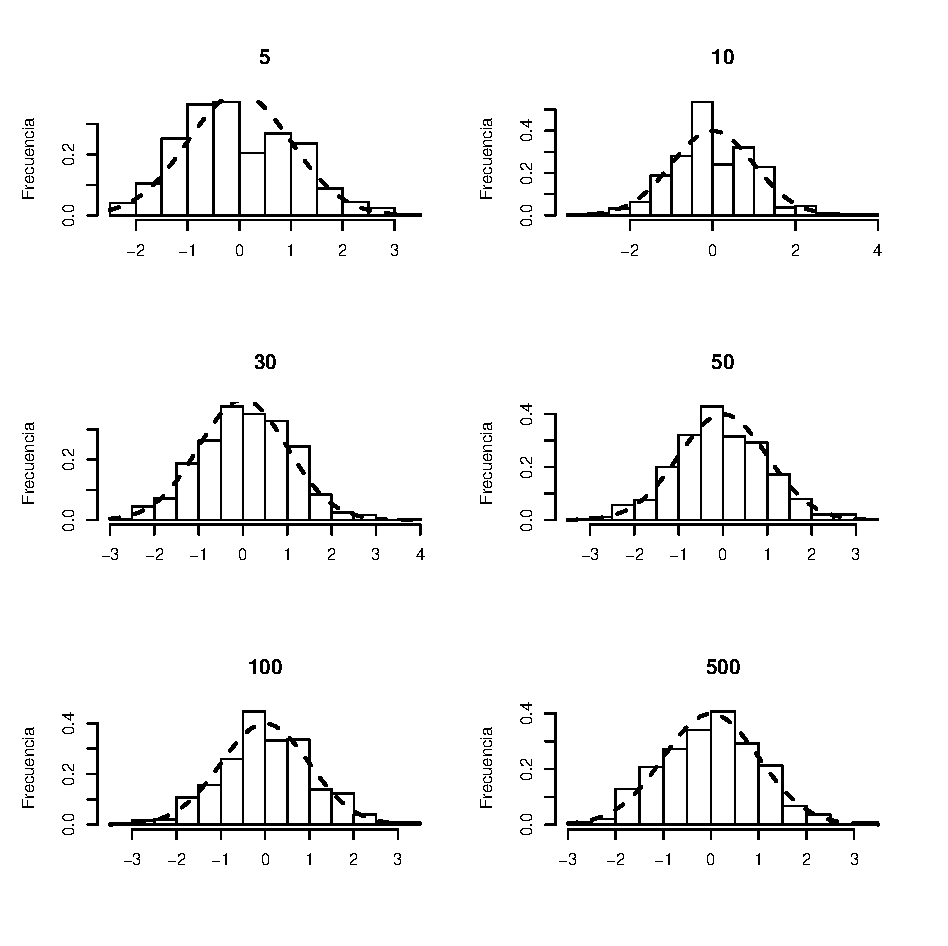
\includegraphics[scale=0.51]{TLC_1.eps}
\caption[\textsl{Distribuci�n de la media en muestras de $Pois(3)$}]{\textsl{Distribuci�n muestral del promedio en muestras con distribuci�n $Pois(3)$ de diferentes tama�os.}}
\end{figure}

\begin{figure}[!htb]
\centering
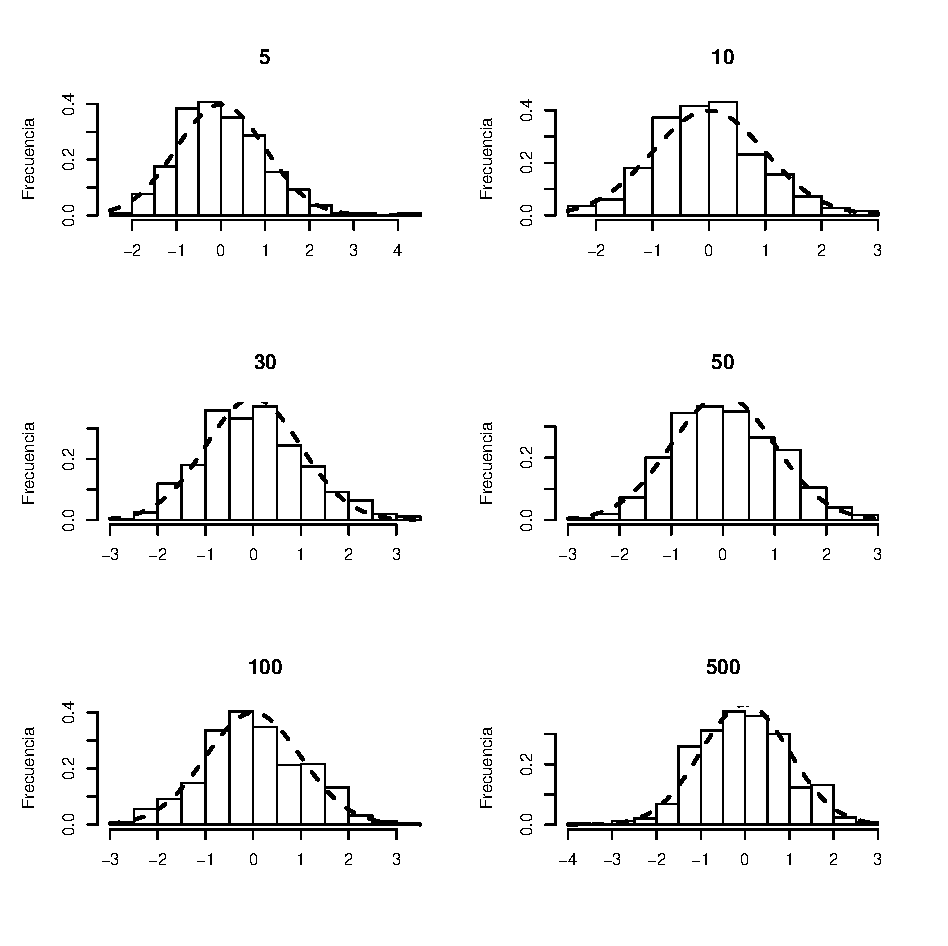
\includegraphics[scale=0.51]{TLC_2.eps}
\caption[\textsl{Distribuci�n de la media en muestras de $Gamma(3,2)$}]{\textsl{Distribuci�n muestral del promedio en muestras con distribuci�n $Gamma(3,2)$ de diferentes tama�os.}}
\end{figure}

\subsubsection{Distribuci�n Ji-cuadrado}

Otra distribuci�n como caso particular de la distribuci�n Gamma es la distribuci�n Ji-cuadrado\index{Distribuci�n!Ji-cuadrado} con $n$ grados de libertad es un caso particular de la distribuci�n Gamma cuando el par�metro de forma $k$ toma el valor $n/2$ para alg�n $n$ entero, y el par�metro de escala $\theta$ toma el valor 2. La funci�n de densidad de la distribuci�n Ji-cuadrado se muestra en la siguiente definici�n.

\begin{Defi}
Una variable aleatoria $X$ tiene distribuci�n Ji-cuadrado con $n$ grados de libertad, con $n$ entero positivo, si su funci�n de densidad est� dada por:
\begin{equation}
f_X(x)=\frac{x^{(n/2)-1}e^{-x/2}}{2^{n/2}\Gamma(n/2)}I_{(0,\infty)}(x),
\end{equation}
y se nota como $X\sim\chi^2_n$.
\end{Defi}

Aunque la distribuci�n Ji-cuadrado es un caso particular de la distribuci�n Gamma, pero �sta est� �ntimamente relacionada con la distribuci�n normal, tal como se muestra en la siguiente definici�n equivalente a la anterior, y resulta ser muy �til en el momento de demostrar que una variable tiene la distribuci�n Ji-cuadrado.

\begin{Defi}
Si $Z_1$, $\cdots$, $Z_n$ son variables aleatorias independientes e id�nticamente distribuidas con distribuci�n normal est�ndar, entonces la variable $\sum_{i=1}^nZ_i^2$ tiene distribuci�n Ji-cuadrado con $n$ grados de libertad.
\end{Defi}

Dado que la distribuci�n $\chi^2$ es un caso particular de la distribuci�n Gamma, la funci�n de densidad tambi�n tiene facetas similares tales como la no simetr�a y la cola larga. En la Figura 1.29 se muestra la funci�n de densidad de distribuci�n $\chi^2_n$ para diferentes valores de $n$.

\begin{figure}[!htb]
\centering
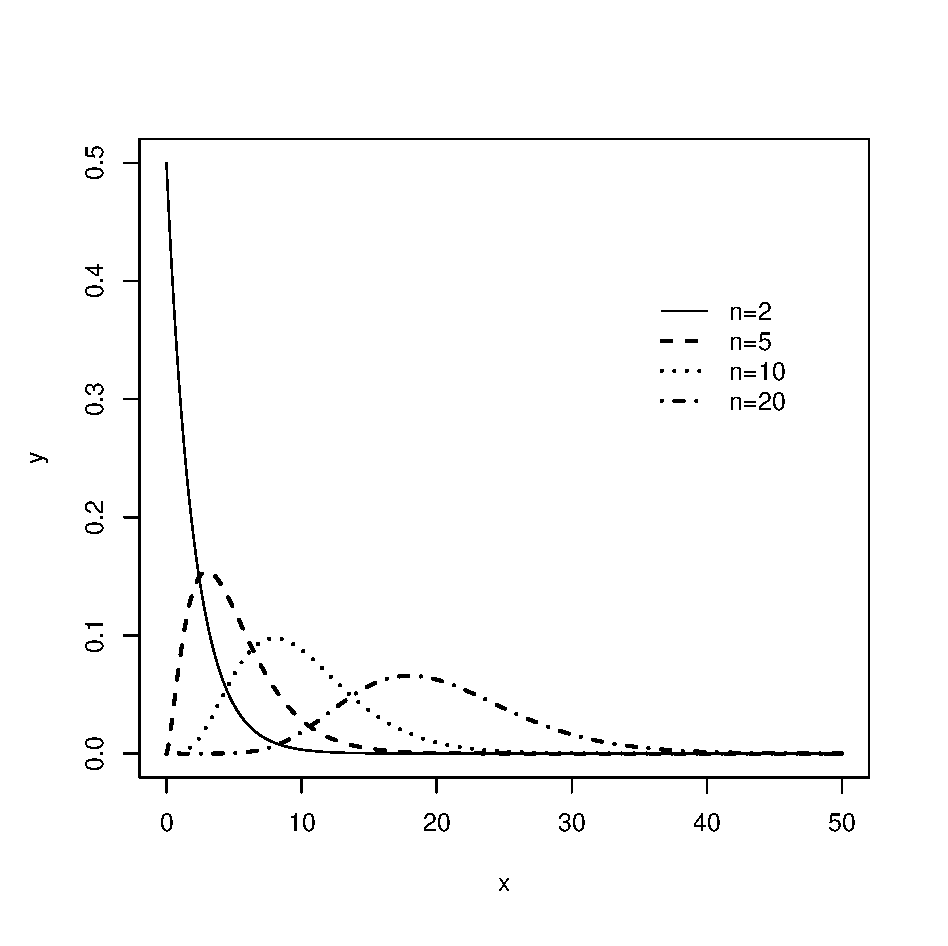
\includegraphics[scale=0.5]{densidad_chi.eps}
\caption[\textsl{Densidad de la distribuciones Ji-cuadrado}]{\textsl{Funci�n de densidad de distribuciones Ji-cuadrado con diferentes grados de libertad.}}
\end{figure}

Usando el Resultado 1.1.12 para la distribuci�n Gamma, se tiene f�cilmente las siguientes propiedades de una variable con distribuci�n Ji-cuadrado.
\begin{Res}
Si $X$ es una variable aleatoria con distribuci�n Ji-cuadro con $n$ grados de libertad, entonces
    \begin{enumerate}
        \item $E(X)=n$.
        \item $Var(X)=2n$.
        \item $m_X(t)=\left(\frac{1}{1-2t}\right)^{n/2}$ para $t<1/2$, y no existe para otros valores de $t$.
    \end{enumerate}
\end{Res}

A continuaci�n se presenta un resultado que nos ser� muy �til en los cap�tulos futuros.

\begin{Res}
Sea $X_1$, $\cdots$, $X_m$ variables aleatorias independientes con distribuci�n $\chi^2_{n_i}$ para $i=1,\cdots,m$, entonces la variable $X=\sum_{i=1}^mX_i$ tiene distribuci�n Ji-cuadrado con $\sum_{i=1}^mn_i$ grados de libertad.
\end{Res}
\begin{proof}
Se har� uso de la funci�n generadora de momentos, tenemos que
\begin{align*}
m_{X}(t)&=E(e^{t\sum_{i=1}^mX_i})\\
&=\prod_{i=1}^nE(e^{tX_i})\\
&=\prod_{i=1}^nm_{X_i}(t)\\
&=\prod_{i=1}^n\left(\frac{1}{1-2t}\right)^{n_i/2}\\
&=\left(\frac{1}{1-2t}\right)^{\sum n_i/2},
\end{align*}
la cual corresponde a la funci�n generadora de momentos de una distribuci�n $\chi^2$ con grado de libertad $\sum_{i=1}^mn_i$, y el resultado queda demostrado.
\end{proof}

El anterior resultado establece que la suma de variables independientes con distribuci�n $\chi^2$ sigue teniendo la distribuci�n $\chi^2$. �Se puede afirmar que la resta de dos variables independientes $\chi^2$ sigue manteniendo la distribuci�n $\chi^2$? Suponga que $X\sim\chi^2_{n_1}$ y $Y\sim\chi^2_{n_2}$ son independientes, y sea $Z=X-Y$, entonces
\begin{align*}
m_Z(t)&=E(e^{t(X-Y)})\\
&=E(e^{tX})/E(e^{tY})\ \ \ \ \ \ \ \text{Por ser $X$ y $Y$ independientes}\\
&=(1-2t)^{-n_1/2}/(1-2t)^{-n_2/2}\\
&=(1-2t)^{-(n_1-n_2)/2},
\end{align*}
la cual corresponde a la funci�n generadora de momentos de una distribuci�n $\chi^2$ con grado de libertad $n_1-n_2$ siempre y cuando $n_1>n_2$. Por lo anterior, podemos afirmar que la resta de dos variables independientes $\chi^2$ sigue teniendo la distribuci�n $\chi^2$ siempre y cuando la resta de los dos grados de libertad sea positiva.

\subsubsection{Distribuci�n $t$-student\index{Distribuci�n!t-student}}
Otra distribuci�n de vital importancia en la teor�a estad�stica es la denominada distribuci�n $t$-student. El descubrimiento de esta distribuci�n fue publicado por  el estad�stico ingl�s William Sealy Gosset (1876-1937) en el a�o 1908 cuando trabajaba en la famosa empresa cervecera Guinness. La publicaci�n la hizo de forma an�nima bajo el nombre de Student, pues Guinness le prohib�a la publicaci�n por ser el descubrimiento parte de resultados de investigaci�n realizada por la empresa. La definici�n de esta distribuci�n se da a continuaci�n.
\begin{figure}[!htb]
\centering
\includegraphics[bb=0 0 427 600, scale=0.3]{Gosset.jpg}
\caption{\textsl{William Sealy Gosset (1876-1937)}}
\end{figure}

\begin{Defi}
Una variable aleatoria $X$ tiene distribuci�n t-student con $n$ grados de libertad si su funci�n de densidad est� dada por:
\begin{equation}\label{densidad_t_central}
f_X(x)=\frac{\Gamma(\frac{n+1}{2})}{\sqrt{\pi n}\ \Gamma(\frac{n}{2})}\left(1+\frac{x^2}{n}\right)^{-(n+1)/2}I_\mathbb{R}(x),
\end{equation}
donde $n>0$ y se nota como $X\sim t_n$.
\end{Defi}
Otra definici�n que se encuentra frecuentemente en la literatura estad�stica es la siguiente, que es m�s �til que la definici�n anterior para demostrar que una variable tiene distribuci�n $t$.

\begin{Defi}
Sea $Z$ una variable aleatoria con distribuci�n normal est�ndar y $Y$ una variable aleatoria con distribuci�n Ji-cuadrado con $n$ grados de libertad, si $Z$ y $Y$ son independientes, entonces la variable $\frac{Z}{\sqrt{Y/n}}$ tiene distribuci�n t-student con $n$ grados de libertad.
\end{Defi}

La funci�n de densidad de la distribuci�n t-student es muy parecida a la de distribuci�n normal est�ndar, tiene la forma de campana de Gauss y sim�trica con respecto al valor 0, adem�s entre m�s grande sea el grado de libertad, m�s se parece a la distribuci�n normal est�ndar. En la Figura 1.31 se muestra la funci�n de densidad de la distribuci�n normal est�ndar y la de distribuci�n $t$ con diferentes grados de libertad donde podemos observar la similitud entre estas distribuciones.

Algunas propiedades de la distribuci�n t-student se muestran en el siguiente resultado.
\begin{Res}
Si $X$ es una variable aleatoria con distribuci�n t-student con $n$ grados de libertad, entonces
    \begin{enumerate}
        \item $E(X)=0$ para $n>1$.
        \item $Var(X)=\frac{n}{n-2}$ para $n>2$.
    \end{enumerate}
\end{Res}

\begin{figure}[!htb]
\centering
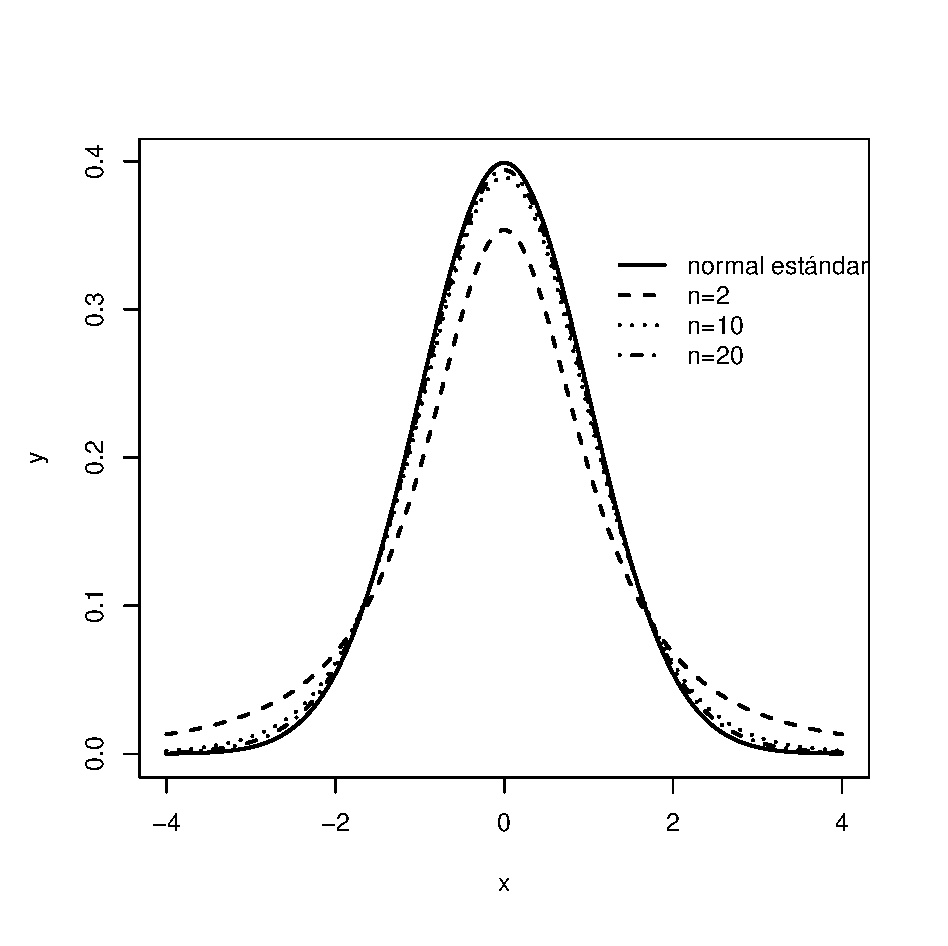
\includegraphics[scale=0.6]{densidad_t.eps}
\caption[\textsl{Densidad de la distribuci�n $N(0,1)$ y $t_2$}]{\textsl{Funciones de densidad de la distribuci�n $N(0,1)$ y $t_n$ con diferentes grados de libertad.}}
\end{figure}

En primer lugar, n�tese que cuando $n$ es grande, la varianza de $X$ se aproxima al valor 1, la varianza de una distribuci�n normal est�ndar. Por otro lado, cabe resaltar que la distribuci�n $t$-student no tiene funci�n generadora de momentos.

\subsubsection{Distribuci�n $t$-student no central\index{Distribuci�n!t-student no central}}
La distribuci�n $t$ student no central es una extensi�n natural de la $t$ student descrita anteriormente\footnote{La distribuci�n con funci�n de densidad (\ref{densidad_t_central}) tambi�n se conoce como la $t$-student central. En este libro se utilizar�n indistintamente estos dos nombres.}, que permte que la esperanza de la distribuci�n normal no sea cero, de all� el t�rmino <<no central>> para esta distribuci�n. An�logo a la distribuci�n $t$ central, existen definiciones equivalentes para la distribuci�n $t$-student no central, las cuales presentamos a continuaci�n.
\begin{Defi}
Una variable aleatoria X tiene distribuci�n $t$-student no central con grados de libertad $n$, y par�metro de no centralidad $\mu$ si su densidad es

\begin{equation*}
f_X(x)=\frac{n^{n/2}\exp\left\{-\frac{n\mu^2}{2(x^2+n)}\right\}}{\sqrt{\pi}\Gamma(n/2)2^{(n-1)/2}(x^2+n)^{(n+1)/2}}\int_{0}^\infty v^n\exp\left\{-\frac{1}{2}\left(v-\frac{\mu x}{\sqrt{x^2+n}}\right)^2\right\}dv
\end{equation*}

y se denota como $X\sim t^{nc}_{n,\mu}$.
\end{Defi}

La funci�n de densidad en la anterior definici�n, es sin duda muy compleja para cualquier c�lculo concerniente a esta distribuci�n. Para efectos de este libro, solo haremos uso de su funci�n de distribuci�n cuyo c�lculo se puede llevar a cabo usando la instrucci�n \verb"pt" en R, m�s adelante explicaremos con detalles sobre el uso de esta funci�n. La otra definici�n equivalente para la distribuci�n $t$-student no central es por medio de construcci�n, y es �til a la hora de probar que cierta variable tiene esta distribuci�n.
\begin{Defi}
Sea $X$ una variable aleatoria con distribuci�n $N(\mu,1)$, y $Y$ una variable aleatoria con distribuci�n Ji-cuadrado con $n$ grados de libertad, si $X$ y $Y$ son independientes, entonces la variable $\frac{X}{\sqrt{Y/n}}$ tiene distribuci�n  $t$-student no central con grados de libertad $n$, y par�metro de no centralidad $\mu$
\end{Defi}

De la anterior definici�n, podemos ver que si $X$ y $Y$ son variables aleatorias independientes con $X\sim N(\mu,\sigma^2)$ y $Y\sim\chi^2_n$ entonces
\begin{equation*}
\frac{X/\sigma}{\sqrt{Y/n}}\sim t^{nc}_{n,\frac{\mu}{\sigma}}.
\end{equation*}

\begin{figure}[!h]
\centering
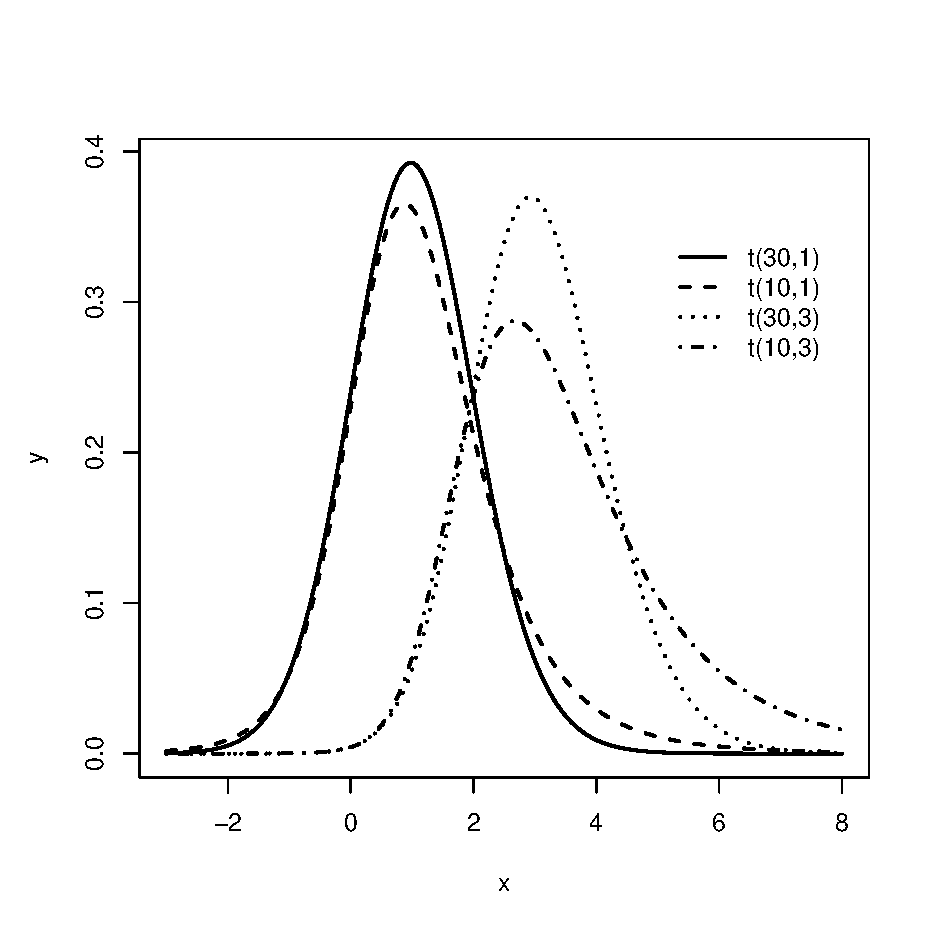
\includegraphics[scale=0.45]{densidad_t_nocentral.eps}
\caption{\textsl{Distintas funciones de densidad $t$-student no central.}}
\end{figure}

\newpage

En la Figura 1.32 se grafica la funci�n de densidad de la distribuci�n $t$-student no central con diferentes grados de libertad y diferentes par�metros de no centralidad. Se puede observar que la esperanza de la distribuci�n $t$ no central es cercana, aunque no igual al par�metro de no centralidad $\mu$; adem�s la funci�n de densidad de esta distribuci�n no es sim�trica, pero se torna m�s sim�trica cuando el grado de libertad es m�s grande.

\subsubsection{Distribuci�n F\index{Distribuci�n!F}}

Otra distribuci�n muy �til es la distribuci�n $F$ que tambi�n se conoce como la distribuci�n F de Fisher o distribuci�n de Fisher-Snedecor, haciendo referencia al gran estad�stico Ronald Aylmer Fisher (1890-1962) y el fundador del primer departamento de estad�stica en los Estados Unidos, George Waddel Snedecor (1881-1974).

\begin{figure}[!h]
\centering
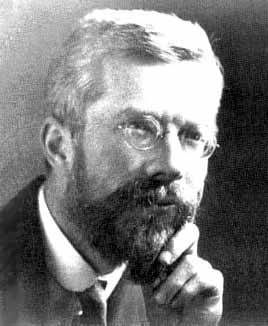
\includegraphics[bb=0 0 268 326, scale=0.4]{Fisher.jpg}
\caption{\textsl{Ronald Aylmer Fisher (1890-1962)}}
\end{figure}

La funci�n de densidad de la distribuci�n F se da en la siguiente definici�n.
\begin{Defi}
Una variable aleatoria $X$ tiene distribuci�n F con $m$ grados de libertad en el numerador y $n$ grados de libertado en el denominador si su funci�n de densidad est� dada por:
\begin{equation}
f_X(x)=\frac{\Gamma(\frac{m+n}{2})}{\Gamma(\frac{m}{2})\Gamma(\frac{n}{2})}\left(\frac{m}{n}\right)^{m/2}\frac{z^{\frac{m}{2}-1}}{\left(1+\frac{m}{n}z\right)^{\frac{m+n}{2}}}I_{(0,\infty)}(x),
\end{equation}
y se nota como $X\sim F^m_n$.
\end{Defi}

Otra definici�n equivalente pero m�s �til de la distribuci�n $F$ es como sigue:

\begin{Defi}
Sea $X$ y $Y$ variables aleatorias independientes con distribuciones Ji-cuadrado con $m$ y $n$ grados de libertad, respectivamente, entonces la variable $\dfrac{X/m}{Y/n}$ tiene distribuci�n F con $m$ grados de libertad en el numerador y $n$ grados de libertado en el denominador.
\end{Defi}

En la Figura 1.34 se observa la funci�n de densidad de la distribuci�n $F$ para di\-fe\-ren\-tes grados de libertad. Podemos observar que �sta es similar a la de una distribuci�n Gamma, no sim�trica con cola larga y en algunos casos similar a la distribuci�n exponencial.

\begin{figure}[!htb]
\centering
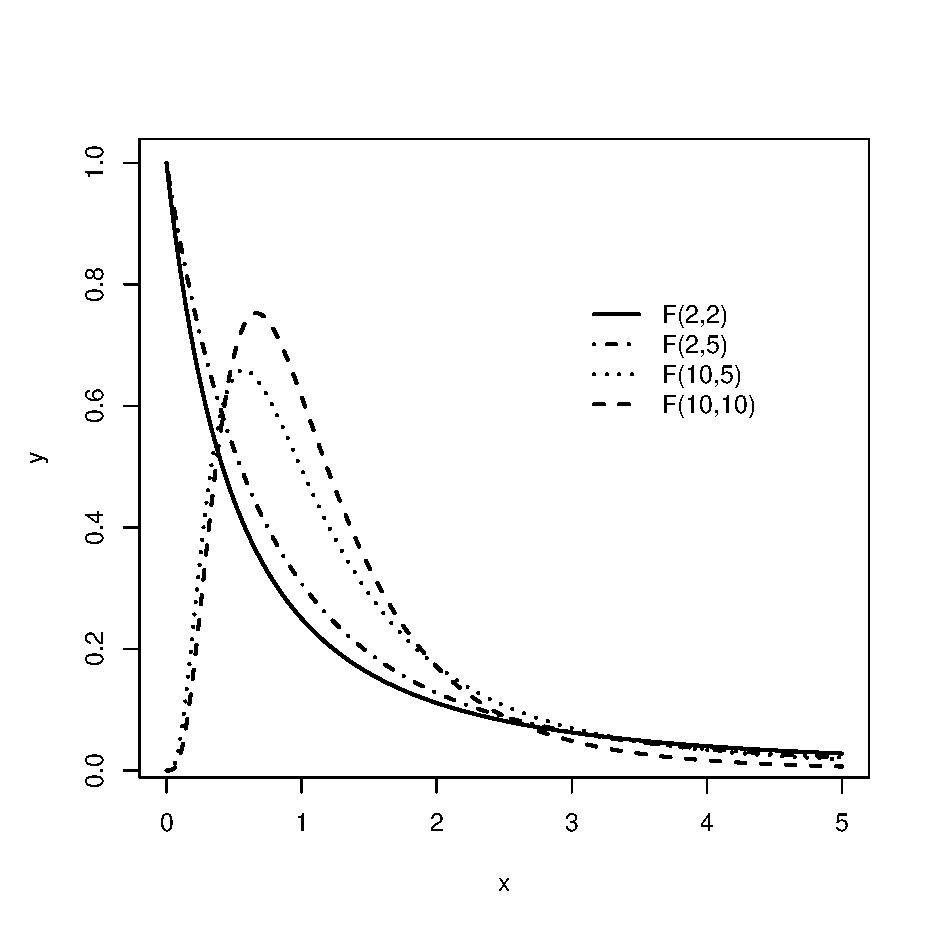
\includegraphics[scale=0.6]{densidad_F.eps}
\caption[\textsl{Densidad de la distribuci�n $F$}]{\textsl{Funciones de densidad de la distribuci�n $F$ con diferentes grados de libertad.}}
\end{figure}

Algunas propiedades de la distribuci�n F se dan a continuaci�n.
\begin{Res}
Si $X$ es una variable aleatoria con distribuci�n F con $m$ grados de libertad en el numerador y $n$ grados de libertado en el denominador, entonces
    \begin{enumerate}
        \item $E(X)=\frac{n}{n-2}$ para $n>2$.
        \item $Var(X)=\frac{2n^2(m+n-2)}{m(n-2)^2(n-4)}$ para $n>4$.
        \item La distribuci�n $F$ no tiene funci�n generadora de momentos.
    \end{enumerate}
\end{Res}

Usando la Definici�n 1.1.19, se tiene f�cilmente el siguiente resultado.
\begin{Res}
Si $X\sim F^m_n$, entonces $1/X\sim F^n_m$.
\end{Res}

\begin{proof}
Trivial usando la Definici�n 1.1.19.
\end{proof}

\subsubsection{Distribuci�n Beta\index{Distribuci�n!Beta}}

La distribuci�n Beta se difiere de las otras distribuciones continuas vistas anteriormente en el sentido de que la distribuci�n Beta solo se usa para describir variables aleatorias que toman valores en el intervalo (0,1). Dado que los datos porcentuales tienen un rango entre 0 y 1\footnote{Cuando un porcentaje es 100\%.}, es com�n pensar que una distribuci�n Beta puede ser apropiada para describir variables aleatorias que representan porcentajes. A continuaci�n damos la definici�n de esta distribuci�n en t�rminos de su funci�n de densidad.
\begin{Defi}
Una variable aleatoria $X$ tiene distribuci�n Beta con par�metros $a>0$ y $b>0$ si su funci�n de densidad est� dada por
\begin{equation}\label{densidad_beta}
f_X(x)=\frac{1}{B(a,b)}x^{a-1}(1-x)^{b-1}I_{(0,1)}(x)
\end{equation}
donde $B(a,b)$ es la funci�n Beta dada por
\begin{equation*}
B(a,b)=\frac{\Gamma(a)\Gamma(b)}{\Gamma(a+b)}=\int_{0}^1u^{a-1}(1-u)^{b-1}du.
\end{equation*}
Usaremos la notaci�n $X\sim Beta(a,b)$ para una variable con esta distribuci�n.
\end{Defi}

\begin{figure}[!htb]
\centering
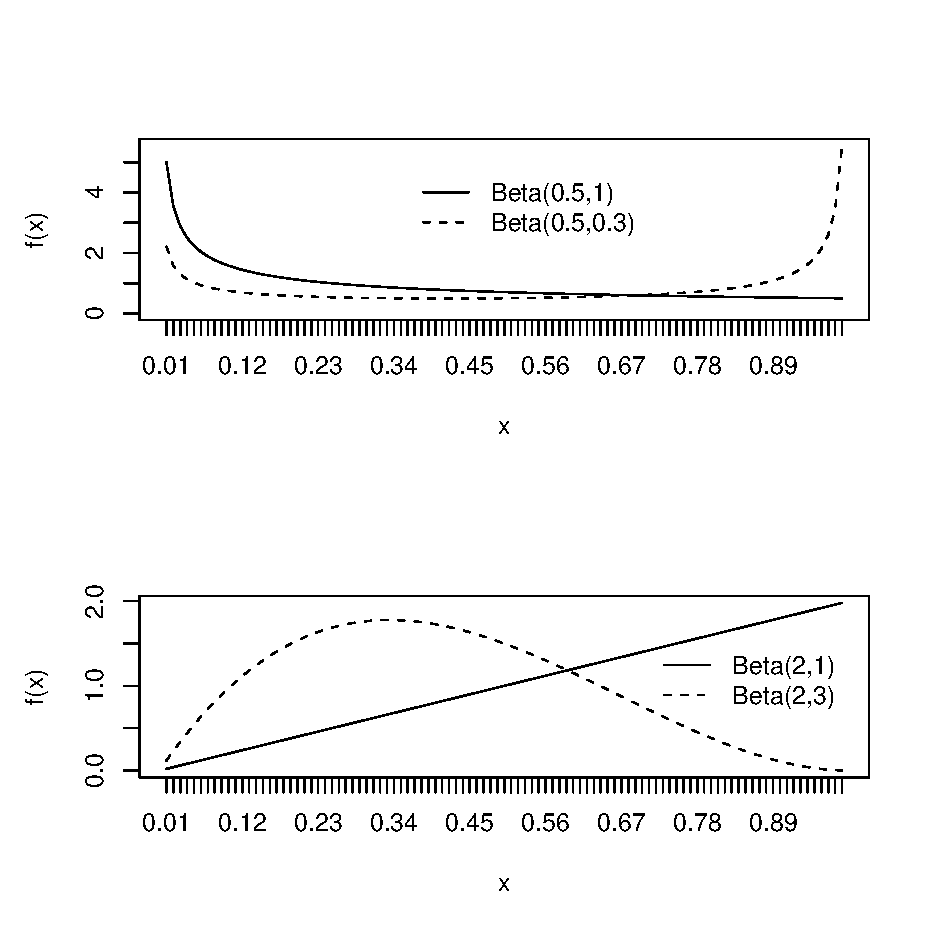
\includegraphics[scale=0.57]{densidad_beta.eps}
\caption{\textsl{Funciones de densidad de algunas distribuciones Beta.}}
\end{figure}

\newpage

Podemos notar que cuando ambos par�metros $a$ y $b$ toman el valor 1, la distribuci�n $Beta(a,b)$ se reduce a una distribuci�n uniforme continua sobre el intervalo $(0,1)$, esto es, $Beta(1,1)=Unif(0,1)$. Por otro lado, podemos ver que la funci�n de densidad de una distribuci�n Beta depende de $x$ por medio de un polinomio de grado $a+b-2$, y la funci�n de densidad toma diversas formas seg�n cambian los par�metros $a$ y $b$. En la Figura 1.35 se muestra la funci�n de densidad de algunas distribuciones Beta. Como puede ver el lector, la funci�n de densidad puede ser una l�nea recta, polinomial, y en algunos casos puede no tener un m�ximo o modas. Esta gran versatilidad permite que la distribuci�n Beta sea apta para describir muchas variables, siempre y cuando �stas toman valores en el intervalo (0,1).

Algunas propiedades de la distribuci�n Beta se enuncian a continuaci�n.
\begin{Res}
Si $X$ es una variable aleatoria con distribuci�n $Beta(a,b)$, entonces
\begin{enumerate}
    \item $E(X)=\frac{a}{a+b}$.
    \item $Var(X)=\frac{ab}{(a+b)^2(a+b+1)}$.
\end{enumerate}
\end{Res}

Observando la forma de la funci�n de densidad de una distribuci�n Beta dada en (\ref{densidad_beta}) podemos observar cierta simetr�a para $f(x)$ y $f(1-x)$, sugiriendo que la variable $1-X$ puede tambi�n tener la distribuci�n Beta si $X$ la tiene. Tenemos el siguiente resultado.

\begin{Res}
Si $X\sim Beta(a,b)$ entonces $Y=1-X\sim Beta(b,a)$.
\end{Res}

\begin{proof}
Una forma de probar lo anterior es encontrando la funci�n de distribuci�n de $Y$, tenemos que para $y\in(0,1)$,
\begin{align*}
F_Y(y)=Pr(Y\leq y)&=Pr(1-X\leq y)\\
&=Pr(X\geq1-y)\\
&=\int_{1-y}^1\frac{x^{a-1}(1-x)^{b-1}}{B(a,b)}dx
\end{align*}
Haciendo un cambio de variables $x=1-u$, tenemos que
\begin{equation*}
F_Y(y)=\int_0^y\frac{(1-u)^{a-1}u^{b-1}}{B(a,b)}dx
\end{equation*}
Y como $B(a,b)=B(b,a)$, podemos concluir que $Y\sim Beta(b,a)$.
\end{proof}

\subsubsection{Relaciones de las distribuciones}

\begin{figure}[!htb]
\centering
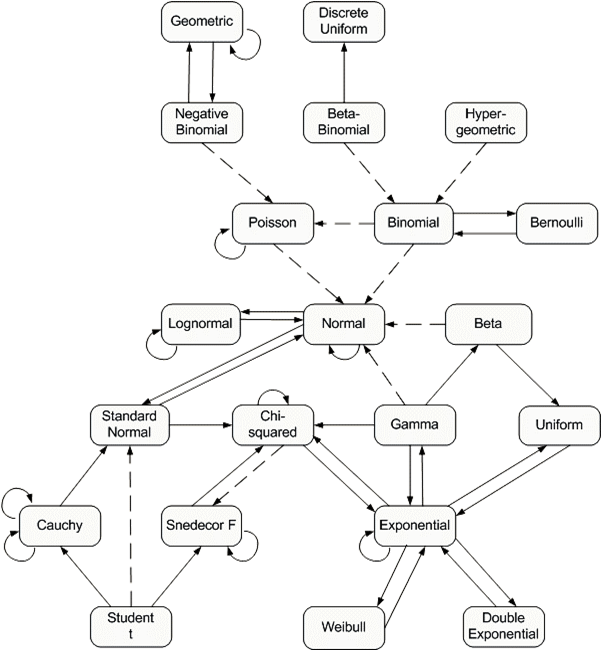
\includegraphics[bb=0 0 602 651, scale=0.5]{relacion.png}
\caption{\textsl{Relaciones entre diferentes distribuciones.}}
\end{figure}

John D. Cook ha elaborado la gr�fica mostrada en la Figura 1.36 acerca de las relaciones de las distribuciones de probabilidad. Seg�n Cook, el gr�fico est� inspirado en \citeasnoun{Lawrence}, en donde los autores muestran en un gr�fico mucho m�s extenso y completo c�mo cada una de las distribuciones de probabilidad univariadas se relacionan y forman familias seg�n las propiedades que tengan.

Entre las propiedades que parametrizan las distribuciones de probabilidad se encuentran las siguientes:

\begin{itemize}
\item Propiedad de combinaci�n lineal: por ejemplo, la suma de variables aleatorias normales independientes resulta tener una distribuci�n normal.
\item Propiedad de convoluci�n: por ejemplo, una variable aleatoria con distribuci�n Ji-cuadrado y con $n$ grados de libertad puede venir de la suma de $n$ variables independientes con distribuci�n Ji-cuadrado y con un grado de libertad.
\item Propiedad del producto: por ejemplo, el producto de variables independientes con distribuci�n lognormales resulta tener una distribuci�n lognormal.
\item Propiedad de la inversa: por ejemplo, si una variable aleatoria tiene distribuci�n $F$, su inversa aritm�tica tambi�n tendr� distribuci�n $F$.
\end{itemize}


\subsection{Percentiles\index{Percentil}}

Un concepto relacionado con las variables aleatorias que es muy importante para la inferencia estad�stica, espec�ficamente la teor�a de intervalo de confianza y las pruebas de hip�tesis, es el concepto del percentil de una variable aleatoria. Definimos este concepto a continuaci�n.

\begin{Defi}
Para una variable aleatoria $X$, el percentil $p$ de $X$, con $0<p<1$, se define como $\inf\{x:\ F_X(x)\geq p\}$ y se denota como $X_p$. Esto es, $X_p$ es el valor m�s peque�o que acumula una probabilidad no inferior de $p$.
\end{Defi}

Para variables aleatorias continuas, la funci�n de distribuci�n correspondiente tambi�n es continua, y existe un �nico punto $x$ con $F(x)=p$, de donde podemos ver que el percentil $p$ de $X$ es simplemente $F^{-1}(p)$.

\begin{Eje}
Sea $X$ una variable aleatoria con distribuci�n $Exp(\theta)$, entonces la funci�n de distribuci�n de $X$ est� dada por
\begin{equation}
F_X(x)=
\begin{cases}
1-e^{-x/\theta}\ \ \ \ \ \text{si $x>0$}\\
0\ \ \ \ \ \ \ \ \ \ \ \ \ \ \ \text{si no}\\
\end{cases}
\end{equation}

Podemos ver que $F_X$ tiene inversa para valores de $x$ en $(0,\infty)$ dada por $F^{-1}(x)=-\theta\ln(1-x)$, con $0<x<1$. De donde podemos calcular el percentil $p$ de la distribuci�n $Exp(\theta)$ como $-\theta\ln(1-p)$. Por ejemplo, el percentil 0.3 de $Exp(4)$ est� dado por $-4\ln(1-0.3)=1.4267$.

Por otro lado, en R, podemos obtener los percentiles de una distribuci�n exponencial con la instrucci�n \verb"qexp" teniendo en cuenta que R utiliza una parametrizaci�n diferente que la de este libro. El comando para calcular el percentil 0.3 de $Exp(4)$ y el resultado es como sigue
\begin{verbatim}
> qexp(0.3,1/4)
[1] 1.426700
\end{verbatim}
\end{Eje}

En algunas distribuciones continuas, como la distribuci�n normal est�ndar, la funci�n de distribuci�n es de una forma muy complicada, y se requiere de algoritmos num�ricos para calcular los percentiles de esta distribuci�n. El comando en R para ese fin es \verb"qnorm" y usa el algoritmo propuesto por \citeasnoun{Wichura}. En este texto, denotaremos el percentil $p$ de una distribuci�n normal est�ndar como $z_p$, y los percentiles comunes que se utilizar�n a lo largo del texto que se encuentran en el ap�ndice G.

Para variables aleatorias discretas, el c�lculo de los percentiles es un poco m�s complicado, puesto que la funci�n de distribuci�n es una funci�n escalonada, y por consiguiente no tiene inversa. Ilustramos el c�lculo en el siguiente ejemplo.

\newpage

\begin{Eje}
Sea $X$ una variable aleatoria con distribuci�n $Bin(8,0.3)$, entonces tenemos que la funci�n de densidad est� dada por
\begin{equation}
f(x)=Pr(X=x)=\begin{cases}
0.058&\text{si $x=0$}\\
0.198&\text{si $x=1$}\\
0.296&\text{si $x=2$}\\
0.254&\text{si $x=3$}\\
0.136&\text{si $x=4$}\\
0.047&\text{si $x=5$}\\
0.01&\text{si $x=6$}\\
0.001&\text{si $x=7$}\\
0.00006&\text{si $x=8$}\\
0&\text{en otro caso}
\end{cases}
\end{equation}

Y su funci�n de distribuci�n est� dada por
\begin{equation}
F(x)=Pr(X\leq x)=\begin{cases}
0&\text{si $x<0$}\\
0.058&\text{si $0\leq x<1$}\\
0.255&\text{si $1\leq x<2$}\\
0.552&\text{si $2\leq x<3$}\\
0.806&\text{si $3\leq x<4$}\\
0.942&\text{si $4\leq x<5$}\\
0.989&\text{si $5\leq x<6$}\\
0.999&\text{si $6\leq x<7$}\\
0.9999&\text{si $7\leq x<8$}\\
1&\text{si $x\geq8$}
\end{cases}
\end{equation}

Suponga que se quiere hallar la mediana de la distribuci�n $Bin(8,0.3)$, esto es, el percentil 50\%, tenemos que
\begin{equation*}
X_{50}=\inf\{x:\ F(x)\geq 0.5\}=\inf\{x:\ x\geq2\}=2
\end{equation*}

N�tese que en este caso, el valor 2 no solo es el percentil 50\%, tambi�n es el percentil 51\%, o 55\%.

El c�mputo de los percentiles en R para la distribuci�n binomial se lleva a cabo usando el comando \verb"qbinom"
\begin{verbatim}
> qbinom(0.5,8,0.3)
[1] 2
\end{verbatim}

\end{Eje}

En muchos textos estad�sticos en la tabla concerniente a la distribuci�n F, s�lo se disponen los percentiles de 90\%, 95\%, 97.5\% y 99\% y no los percentiles 10\%, 5\%, 2.5\% y 1\%. Sin embargo, por el Resultado 1.1.28, se puede ver f�cilmente que el percentil $\alpha$ de una distribuci�n $F^{n}_m$ es simplemente la inversa del percentil $1-\alpha$ de la distribuci�n $F^{m}_n$. Para ver eso, suponga que $X\sim F^m_n$, y denotamos el percentil $\alpha$ de $X$ como $f^m_{n,\alpha}$, entonces tenemos que
\begin{equation*}
\alpha=Pr(X<f^m_{n,\alpha})=Pr\left(\frac{1}{X}>\frac{1}{f^m_{n,\alpha}}\right)=1-Pr\left(\frac{1}{X}<\frac{1}{f^m_{n,\alpha}}\right)
\end{equation*}

De donde tenemos que $1-\alpha=Pr\left(\frac{1}{X}<\frac{1}{f^m_{n,\alpha}}\right)$, y vemos que $\frac{1}{f^m_{n,\alpha}}$ es el percentil de $1/X$ que se distribuye como $F^n_m$. De lo anterior, $\frac{1}{f^m_{n,\alpha}}=f^n_{m,1-\alpha}$, y finalmente tenemos que $f^m_{n,\alpha}=\frac{1}{f^n_{m,1-\alpha}}$.

En la Tabla 1.1 presentamos los comandos en R para calcular percentiles. Tambi�n presentamos algunos percentiles usuales de las distribuciones $t$ student, Ji-cuadrado y F al final de este cap�tulo.

\begin{table}[!htb]
\centering
{\small
\begin{tabular}{|c|c|c|c|}\hline
Distribuci�n&Comando&\multicolumn{2}{|c|}{Ejemplo}\\\hline
$Bin(n,p)$&\verb"qbinom"&Percentil 0.1 de $Bin(12,0.4)$&\verb"qbinom(0.1,12,0.4)"\\
$Pois(\lambda)$&\verb"qpois"&Percentil 0.2 de $Pr(5)$&\verb"qpois(0.2,5)"\\
$U(a,b)$&\verb"qunif"&Percentil 0.3 de $U(3,6)$&\verb"qunif(0.3,3,6)"\\
$Gammma(k,\theta)$&\verb"qgamma"&Percentil 0.4 de $Gamma(2,8)$&\verb"qgamma(0.4,2,8)"\\
$Exp(\theta)$&\verb"qexp"&Percentil 0.5 de $Exp(2)$&\verb"qexPr(0.5,1/2)"\\
$N(\mu,\sigma^2)$&\verb"qnorm"&Percentil 0.6 de $N(2,9)$&\verb"qnorm(0.6,2,sqrt(9))"\\
$N(0,1)$&\verb"qnorm"&Percentil 0.7 de $N(0,1)$&\verb"qnorm(0.7)"\\
$t_n$&\verb"qt"&Percentil 0.8 de $t_{20}$&\verb"qt(0.8,20)"\\
$\chi^2_n$&\verb"qchisq"&Percentil 0.9 de $\chi^2_{25}$&\verb"qchisq(0.9,25)"\\
$F^m_n$&\verb"qf"&Percentil 0.95 de $F^{11}_{12}$&\verb"qf(0.95,11,12)"\\\hline
\end{tabular} }
\caption[\textsl{Comandos en R para c�lculo de percentiles}]{\textsl{Comandos en R para c�lculo de percentiles en las distribuciones de uso frecuente.}}
\end{table}


\section{Familia exponencial}

En este apartado, se introduce el concepto de familia exponencial que es muy �til en algunos temas tratados en este libro, como son la teor�a de estimaci�n puntual y prueba de hip�tesis; as� mismo, resulta �til en la teor�a bayesiana que, sin embargo, no ser� tratada en este libro.

\subsection{Familia exponencial uniparam�trica\index{Familia exponencial!uniparam�trica}}

En esta parte, se introduce la familia exponencial para distribuciones que depende solamente de un par�metro que se denominar� familia exponencial uniparam�trica, cuya definici�n se da a continuaci�n.

\begin{Defi}
Una distribuci�n de probabilidad con par�metro $\theta$ pertenece a la familia exponencial uniparam�trica si la funci�n de densidad se puede escribir de la forma
    \begin{equation}\label{uniexpo}
    f_X(x,\theta)=h(x)c(\theta)\exp\{d(\theta)T(x)\}
    \end{equation}
donde $T(x)$ y $h(x)$ son funciones que dependen de $x$ �nicamente, y $d(\theta)$ y $c(\theta)$ son funciones que dependen de $\theta$ �nicamente.
\end{Defi}

En algunos textos, la representaci�n de la familia exponencial es $f_X(x,\theta)=\exp\{d(\theta)T(x)-c(\theta)\}h(x)$, la cual es equivalente a la definici�n anterior. A con\-ti\-nua\-ci�n se ilustra dos ejemplos de distribuciones pertenecientes a esta familia.

\begin{Eje}
La distribuci�n Poisson con par�metro $\theta$ pertenece a la familia exponencial uniparam�trica puesto que
\begin{align*}
f(x,\theta)&=\frac{e^{-\theta}\theta^x}{x!}I_{\{0,1,\cdots\}}(x)\\
           &=\exp\{x\ln\theta\}\exp\{-\theta\}\frac{I_{0,1,\cdots}(x)}{x!},
\end{align*}
en conclusi�n $f(x,\theta)$ es de la forma (\ref{uniexpo}) con $d(\theta)=\ln\theta$, $T(x)=x$, $c(\theta)=\exp\{-\theta\}$ y $h(x)=\dfrac{I_{\{0,1,\cdots\}}(x)}{x!}$.
\end{Eje}

\begin{Eje}
La distribuci�n Gamma con par�metro de forma $k$ conocida pertenece a la familia exponencial uniparam�trica puesto que
\begin{align*}
f(x,\theta)&=\frac{x^{k-1}e^{-x/\theta}}{\theta^k\Gamma(k)}I_{(0,\infty)}(x)\\
           &=\exp\left\{-\frac{x}{\theta}\right\}\theta^{-k}\frac{x^{k-1}I_{(0,\infty)}(x)}{\Gamma(k)},
\end{align*}
el cual es de la forma (\ref{uniexpo}) con $d(\theta)=-1/\theta$, $T(x)=x$, $c(\theta)=\theta^{-k}$ y $h(x)=\dfrac{x^{k-1}I_{(0,\infty)}(x)}{\Gamma(k)}$.

N�tese que esta representaci�n de la familia exponencial no es �nica, puesto que al definir $d(\theta)=1/\theta$ y $T(x)=-x$, tambi�n se puede concluir que la distribuci�n Gamma con $k$ fijo pertenece a la familia exponencial uniparam�trica.
\end{Eje}

En casi toda la teor�a estad�stica, se trata m�s de una variable aleatoria que en la pr�ctica, se observan los datos que corresponden a realizaciones de estas variables. En este caso, se examina la pertenencia de la familia exponencial de la funci�n de densidad conjunta, y tenemos el siguiente resultado.
\begin{Res}
Si $X_1$, $\cdots$, $X_n$ son variables aleatorias independientes e id�nticamente distribuidas con funci�n de densidad com�n perteneciente a la familia exponencial uniparam�trica, entonces la funci�n de densidad conjunta $f(x_1,\cdots,x_n)$ tambi�n pertenece a la familia exponencial uniparam�trica.
\end{Res}
\begin{proof}
\begin{align}\label{exponencial_muestra}
f(x_1,\cdots,x_n,\theta)&=\prod_{i=1}^nf(x_i,\theta)\notag\\
                        &=\prod_{i=1}^nh(x_i)c(\theta)\exp\{d(\theta)T(x_i)\}\notag\\
                        &=c(\theta)^n\left[\prod_{i=1}^nh(x_i)\right]\exp\left\{d(\theta)\sum_{i=1}^nT(x_i)\right\}
\end{align}
el cual es de la forma (\ref{uniexpo}).
\end{proof}

Usando el anterior resultado junto con el Ejemplo 1.2.1, donde se mostr� que la distribuci�n Poisson pertenece a la familia exponencial, podemos afirmar que cuando se tiene $n$ variables independientes e id�nticamente distribuidas con distribuci�n Poisson, la funci�n conjunta tambi�n pertenece a la familia exponencial.

Otra utilidad del resultado es que cuando se necesita ver que una funci�n de densidad conjunta pertenece a la familia exponencial, basta ver para la funci�n de densidad marginal.

La estad�stica $\sum_{i=1}^nT(x_i)$ en (\ref{exponencial_muestra}) ser� de gran inter�s en los futuros cap�tulos, y estamos interesados en conocer sus propiedades como la esperanza y la varianza, y para eso solo necesitamos $E(T(X))$ y $Var(T(X))$ para $X$ con la misma distribuci�n que $X_1$, $\cdots$, $X_n$. El siguiente resultado nos provee las respectivas f�rmulas.

\begin{Res}
Si $X$ es una variable aleatoria con funci�n de densidad perteneciente a la familia exponencial de la forma (\ref{uniexpo}), entonces
\begin{enumerate}
    \item $E\left(\dfrac{\partial d(\theta)}{\partial\theta}T(X)\right)=-\dfrac{\partial}{\partial\theta}\ln c(\theta)$
    \item $Var\left(\dfrac{\partial d(\theta)}{\partial\theta}T(X)\right)=-\dfrac{\partial^2}{\partial\theta^2}\ln c(\theta)-E\left(\dfrac{\partial^2d(\theta)}{\partial\theta^2}T(X)\right)$
\end{enumerate}
\end{Res}

Ahora, las distribuciones con dos par�metros, como la distribuci�n $N(\mu,\sigma^2)$, pueden considerarse como distribuci�n uniparam�trica cuando $\mu$ o $\sigma^2$ se considera fijo conocido. Y se puede ver que en ambos casos, la distribuci�n pertenece a la familia exponencial uniparam�trica.

\subsection{Familia exponencial multi-param�trica\index{Familia exponencial!multi-param�trica}}

Las distribuciones Gamma, normal y beta dependen de dos par�metros, y para estas distribuciones, se puede generalizar la definici�n de la familia exponencial uniparam�trica para distribuciones dependientes de m�s de un par�metro. La definici�n correspondiente se da a continuaci�n.
\begin{Defi}
Una distribuci�n de probabilidad pertenece a la familia exponencial multi-param�trica si la funci�n de densidad se puede escribir de la forma
    \begin{equation}\label{multiexpo}
    f_X(x,\btheta)=c(\btheta)h(x)\exp\{d(\btheta)'T(x)\}
    \end{equation}
donde $T(x)$ y $d(\btheta)$ son funciones vectoriales, $h(x)$ y $c(\btheta)$ son funciones reales.
\end{Defi}

\begin{Eje}
La distribuci�n Gamma con par�metro de forma $k$ y par�metro de escala $\theta$ pertenece a la familia exponencial multi-param�trica pues
\begin{align*}
f_X(x)&=\frac{x^{k-1}e^{-x/\theta}}{\theta^k\Gamma(k)}I_{(0,\infty)}(x)\\
      &=\exp\left\{-\frac{x}{\theta}+(k-1)\ln{x}\right\}\frac{1}{\theta^k\Gamma(k)}I_{(0,\infty)}(x)\\
      &=\exp\left\{\Bigl(-\frac{1}{\theta},k-1\Bigr)\begin{pmatrix}x\\ \ln{x}\end{pmatrix}\right\}\frac{1}{\theta^k\Gamma(k)}I_{(0,\infty)}(x)
\end{align*}
el cual es de la forma (\ref{multiexpo}) con $\btheta=(\theta,k)'$, $d(\btheta)=(-\frac{1}{\theta},k-1)'$,
$c(\btheta)=\frac{1}{\theta^k\Gamma(k)}$, $T(x)=(x,\ln{x})'$ y $h(x)=I_{(0,\infty)}(x)$.
\end{Eje}

N�tese que al igual a la familia exponencial uniparam�trica, la representaci�n de la familia exponencial multi-param�trica tampoco es �nica, pues en el ejemplo anterior tambi�n se puede tomar
$\eta(\mathbf{\theta})=(\frac{1}{\theta},k-1)'$ y $T(x)=(-x,\ln{x})'$.

Las distribuciones normal, gamma, exponencial, Ji-cuadrado, beta, Bernoulli, binomial, binomial negativa, multinomial, Poisson y geom�trica, pertenecen todas a la familia exponencial. Tambi�n la distribuci�n Weibull pertenece a la familia exponencial cuando el par�metro de forma es conocido. Por otra parte, las distribuciones Cauchy, Laplace, uniforme y Weibull cuando el par�metro de forma es desconocido no pertenecen a la familia exponencial.

La raz�n por la que las distribuciones de la familia uniforme no pertenecen a la familia exponencial va m�s all� de los objetivos de este libro,
pues se necesita conocimientos sobre teor�a estad�stica basada en la teor�a de la medida. La afirmaci�n  de que la distribuci�n uniforme no pertenece a la familia exponencial porque no se puede escribir de la forma (\ref{multiexpo}) no es una raz�n v�lida.

\section{Ejercicios}
\begin{enumerate}[{1}.1]

\item Demuestre el Resultado 1.1.1.

\item La funci�n de densidad de una variable $X$ con distribuci�n Bernoulli tambi�n se puede escribir como
\begin{equation*}
f_X(x)=\begin{cases}
p&\text{si $x=1$}\\
1-p&\text{si $x=0$}\\
0&\text{si no}
\end{cases}
\end{equation*}
Verifique que esta funci�n coincide con la funci�n de densidad dada en (\ref{densidad_Bernoulli}).

\item Un vendedor de seguros realiza en promedio 10 visitas por semana a los posibles clientes, �l por experiencia sabe que la probabilidad de que un cliente compre el seguro en una visita es de 0.2, y suponga que el resultado de una visita no se ve afectado por resultados de visitas anteriores.
    \begin{enumerate}[(a)]
        \item �Cu�l es la probabilidad de que el vendedor en una semana venda m�s de dos seguros?
        \item Suponga que el vendedor ha tenido semanas consecutivas con muy malas ventas, y que perder� el trabajo si en la pr�xima semana no vende por lo menos un seguro. Por lo tanto, el vendedor decide aumentar el n�mero de visitas a la semana para tratar al menos un seguro, �por lo menos cu�ntas visitas debe realizar la pr�xima semana para que la probabilidad de vender al menos un seguro sea superior a 90\%?
    \end{enumerate}

\item Demuestre el Resultado 1.1.3.

\item Para la distribuci�n exponencial, escriba cu�l es el par�metro y cu�l es el espacio param�trico.

\item Demuestre el Resultado 1.1.7.

\item Demuestre el Resultado 1.1.9.

\item Demuestre el Resultado 1.1.11.

\item Demuestre el Resultado 1.1.13.

\item Demuestre que la funci�n de densidad de la distribuci�n $N(\mu,\sigma^2)$ cumple las siguientes propiedades
\begin{enumerate}[(a)]
    \item sim�trica con respecto a $\mu$,
    \item es creciente para $x<\mu$ y decreciente para $x>\mu$ y por consiguiente, tiene un m�ximo en $\mu$.
\end{enumerate}

\item Demuestre que si $X\sim N(\mu,\sigma^2)$ entonces $E(X)=\mu$ y $Var(X)=\sigma^2$ usando la funci�n generadora de momentos de $X$ dada en el Resultado 1.1.19.

\item Sea $X\sim N(\mu,\sigma^2)$, y sea $Z_1=\frac{X-\mu}{\sigma}$ y $Z_2=\frac{\mu-X}{\sigma}$, usando el Resultado 1.1.20 compruebe que tanto $Z_1$ como $Z_2$ tienen distribuci�n normal est�ndar, es decir, la forma de estandarizar una variable con distribuci�n normal no es �nica.

\item Demuestre el Resultado 1.1.21.

\item Demuestre el Resultado 1.1.22.

\item Calcule las siguientes probabilidades:
\begin{enumerate}[(a)]
    \item $Pr(X>2)$, $Pr(X<-1)$ y $Pr(1<X<3)$ donde $X\sim N(1.5,4)$.
    \item $Pr(\frac{X-2Y}{3}>4)$ donde $X\sim N(1.5,4)$ y $Y\sim N(-1,2)$ son variables independientes.
\end{enumerate}

\item Para $X_1$, $\cdots$, $X_n$ independientes e id�nticamente distribuidas provenientes de las siguientes distribuciones, escriba cu�l ser� la variable $\sqrt{n}(\bar{X}-\mu)/\sigma$ en el contexto del Resultado 1.1.23.

\item Para las distribuci�n Ji-cuadrado, escriba cu�l es el par�metro y cu�l es el espacio param�trico.

\item Si $X\sim\chi^2_{n}$, demuestre que $E(X)=n$ y $Var(X)=2n$ usando la Definici�n 1.1.13.

\item  \begin{enumerate}[(a)]
    \item Calcule el percentil 5\%, 10\% y 98\% de una variable con distribuci�n normal est�ndar.
    \item Calcule el percentil 5\% y 90\% de una variable con distribuci�n $N(1,3)$.
    \item Encuentre valores $a$ y $b$ tales que $Pr(a<Z<b)=0.98$.
    \item Encuentre valores $a$ y $b$ tales que $Pr(a<X<b)=0.95$ donde $X\sim N(-2,5)$.
\end{enumerate}

\item Comprobar que en una distribuci�n normal est�ndar $z_p=-z_{1-p}$, corrobora lo anterior calculando estos percentiles con los comandos dados en la Tabla 1.1. con un valor $p$ fijo.

\item Encuentre los percentiles 5\%, 98\% de una variable con distribuci�n Ji-cuadrado con 8 y 15 grados de libertad, respectivamente.

\item Encuentre los percentiles 5\%, 98\% de una variable con distribuci�n t-student con 10 y 20 grados de libertad, respectivamente.

\item Encuentre los percentiles 5\%, 98\% de una variable con distribuci�n $F_5^8$ y $F_8^{12}$, respectivamente.

\item Demuestre que las siguientes distribuciones pertenecen a la familia exponencial identificando las funciones $d(\theta)$, $T(x)$, $c(\theta)$ y $h(x)$:
\begin{enumerate}[(a)]
    \item Binomial con $n$ conocido.
    \item Exponencial.
    \item Distribuci�n normal con media $\mu$ conocido.
    \item Distribuci�n normal con varianza $\sigma^2$ conocida.
    \item La funci�n de densidad conjunta de $X_1$, $\cdots$, $X_n$, donde las variables $X_i$ son independientes e id�nticamente distribuidas con distribuci�n com�n $N(\mu,\sigma^2)$ con $\mu$ conocido (primero directamente y luego usando el Resultado 1.2.1.).
    \item La funci�n de densidad conjunta de $X_1$, $\cdots$, $X_n$ donde las variables $X_i$ son independientes e id�nticamente distribuidas con distribuci�n com�n $Pois(\lambda)$ (primero directamente y luego usando el Resultado 1.2.1.).
\end{enumerate}

\item Demuestre la distribuci�n Weibull, cuando $k$ es conocido, pertenece a la familia exponencial uniparam�trica. Identifique $d(\theta)$, $T(x)$, $c(\theta)$ y $h(x)$.

\item Demuestre que la distribuci�n $N(\mu,\sigma^2)$ pertenece a la familia exponencial multiparam�trica. Identifique $d(\btheta)$, $T(x)$, $c(\btheta)$ y $h(x)$.

\item Demuestre que la distribuci�n Beta pertenece a la familia exponencial multiparam�trica. Identifique $d(\btheta)$, $T(x)$, $c(\btheta)$ y $h(x)$.

\item Sean $X_1$, $\cdots$, $X_n$ variables aleatorias independientes e id�nticamente distribuidas con distribuci�n com�n, $N(\mu_1,\sigma^2_1)$ y $Y_1$, $\cdots$, $Y_m$ variables independientes e id�nticamente distribuidas con distribuci�n com�n $N(\mu_2,\sigma^2_2)$, adem�s las variables $X_i$ son independientes de las variables $Y_j$, demuestre que la funci�n de densidad conjunta de $X_1$, $\cdots$, $X_n$, $Y_1$, $\cdots$, $Y_m$ pertenece a la familia exponencial.

\item Repita el punto anterior suponiendo que $\sigma^2_1=\sigma^2_2=\sigma^2$.

\end{enumerate} 
\chapter[Estimaci�n puntual]{Estimaci�n puntual}

\section{Introducci�n}

Desde la revoluci�n estad�stica de Pearson y Fisher, la inferencia estad�stica busca encontrar los valores que parametrizan a la distribuci�n desconocida de los datos. El primer enfoque, propuesto por Pearson, afirmaba que si era posible observar a la variable de inter�s en todos y cada uno de los individuos de una poblaci�n, entonces era posible calcular los par�metros de la distribuci�n de la variable de inter�s; por otro lado, si s�lo se ten�a acceso a una muestra representativa, entonces era posible calcular una estimaci�n de tales par�metros.

Fisher discrep� de tales argumentos, asumiendo que las observaciones est�n sujetas a un error de medici�n y por lo tanto, as� se tuviese acceso a toda la poblaci�n, es imposible calcular los par�metros de la distribuci�n de la variable de inter�s.

Del planteamiento de Fisher resultaron una multitud de m�todos estad�sticos para la estimaci�n de los par�metros te�ricos. Es decir, si la distribuci�n de $ X$ est� para\-me\-tri\-za\-da por $ \theta \in \Theta$, con $ \Theta$ el espacio param�trico inducido por el comportamiento de la variable de inter�s, el objetivo de la teor�a estad�stica inferencial es calcular una estimaci�n $ \hat{\theta}$ del par�metro $ \theta$ por medio de los datos observados. En este enfoque, los par�metros se consideran cantidades fijas y constantes. 

El anterior ser� el enfoque que seguiremos a lo largo del desarrollo de este libro, aunque el lector debe tener conocimiento de que no es el �nico enfoque que los estad�sticos utilizan en t�rminos de inferencia acerca de los par�metros de una distribuci�n.

N�tese que en t�rminos de inferencia estad�stica existen, por lo menos, el enfoque cl�sico, propuesto por Fisher y desarrollado en este libro, el enfoque bayesiano \cite{Gelman}, el enfoque no param�trico \cite{Conover98} y el enfoque de inferencia en poblaciones finitas \cite{Gutierrez}.

\section{Conceptos b�sicos}

Muchos de los estudios estad�sticos est�n enfocados en estudiar caracter�sticas de una poblaci�n objetiva; por ejemplo, una empresa productora puede estar interesada en conocer el gasto promedio semanal en alimentos de las familias de estrato so\-cio\-eco\-n�\-mi\-co bajo, con el fin de dise�ar una estrategia de mercadeo para promover la demanda en el mercado. Es claro que en la ciudad hay una gran cantidad de familias de este perfil, y por consiguiente resulta pr�cticamente imposible saber el gasto promedio semanal de cada una de estas familias.

En casos como el anterior, la soluci�n es inferir acerca de la caracter�stica de la poblaci�n usando informaci�n obtenida de un subconjunto o una muestra de la poblaci�n, y t�cnicas de esta rama constituyen la inferencia estad�stica. A continuaci�n se presentan algunos conceptos b�sicos para poder estudiar la teor�a de la inferencia estad�stica.
\begin{Defi}
Una muestra aleatoria\index{Muestra aleatoria} de tama�o $n$ es un conjunto constituido por $n$ variables aleatorias independientes e id�nticamente distribuidas, $X_1$, $\cdots$,$X_n$.
\end{Defi}

Una muestra aleatoria es utilizada para lograr el objetivo de estimar un par�metro te�rico desconocido, y esto se logra usando una funci�n o funciones de las variables aleatorias de la muestra, conocidas como estad�sticas. La definici�n formal se enuncia a continuaci�n.
\begin{Defi}
Una estad�stica\index{Estad�stica} es una funci�n de variables aleatorias de una muestra aleatoria que no contiene par�metros desconocidos.
\end{Defi}

Algunas estad�sticas comunes basadas en una muestra aleatoria $X_1$, $\cdots$m $X_n$ son:
\begin{itemize}
\item El promedio muestral o la media muestral\index{Media muestral}, definido como $\bar{X}=\sum_{i=1}^nX_i/n$.
\item Las varianzas muestrales, definidas como $S^2_{n}=\sum_{i=1}^n(X_i-\bar{X})^2/n$ y $S^2_{n-1}=\sum_{i=1}^n(X_i-\bar{X})^2/(n-1)$.
\item M�nimo y m�ximo de la muestra\index{M�nimo de una muestra}\index{M�ximo de una muestra}, definidos como $X_{(1)}=\min\{X_1,\cdots,X_n\}$ y $X_{(n)}=\max\{X_1,\cdots,X_n\}$. N�tese que en general la estad�stica $X_{(1)}$, al igual que $X_{(n)}$, no es ninguna de las variables $X_1$, $\cdots$, $X_n$. Considere un experimento aleatorio con $\Omega=\{a,b,c\}$ y se definen dos variables aleatorias $X_1$ y $X_2$ sobre $\Omega$ con $X_1(a)=X_1(b)=1$, $X_1(c)=2$ y $X_2(a)=0$, $X_2(b)=X_2(c)=2$. Si denotamos al m�nimo de $X_1$ y $X_2$ como $Y$, se puede ver que $Y(a)=0$, $Y(b)=1$ y $Y(c)=2$, y claramente $Y$ no es ninguna de las variables $X_1$ y $X_2$. De esta forma si la funci�n de densidad de donde proviene la muestra es $f_X$, la funci�n de densidad de $X_{(1)}$ y la de $X_{(n)}$ no corresponden a $f_X$.
    Veamos
    \begin{align*}
    Pr(X_{(1)}>x)&=Pr(X_1>x,\cdots,X_n>x)\\
    &=Pr(X_1>x)\cdots Pr(X_n>x)\\
    &=(1-F_{X_1}(x))\cdots (1-F_{X_n}(x))\\
    &=(1-F_X(x))^n
    \end{align*}
    donde $F_X$ denota la funci�n de distribuci�n com�n de la muestra. Por otro lado, $Pr(X_{(1)}>x)=1-F_{X_{(1)}}(x)$, de esta forma, tenemos que
    \begin{equation*}
        F_{X_{(1)}}(x)=1-(1-F_X(x))^n,
    \end{equation*}
    y podemos hallar la funci�n de densidad para encontrar la funci�n de densidad de $X_{(1)}$ como
    \begin{equation}
        f_{X_{(1)}}(x)=nf_X(x)(1-F_X(x))^{n-1}.
    \end{equation}
    Usando lo anterior, podemos encontrar que la funci�n de densidad de $X_{(1)}$ en una muestra con distribuci�n exponencial de media $\theta$, corresponde a
    \begin{equation*}
        f_{X_{(1)}}(x)=\frac{n}{\theta}e^{-nx/\theta}I_{(0,\infty)}(x).
    \end{equation*}
    Usando un razonamiento an�logo, se puede ver (Ejercicio 2.1) que para la estad�stica m�ximo $X_{(n)}$, se tiene que
    \begin{equation}\label{F_max}
        F_{X_{(n)}}(x)=F_X(x)^n
    \end{equation}
    y
    \begin{equation}\label{f_max}
        f_{X_{(n)}}(x)=nf_X(x)F_X(x)^{n-1}.
    \end{equation}
\end{itemize}

Una vez definido el concepto de estad�stica, podemos definir lo que es un estimador. Aunque en muchos contextos, lo que se desea estimar es el par�metro de una distribuci�n, $\theta$, en algunos casos, lo que nos interesa es una funci�n del par�metro $g(\theta)$. Por ejemplo, suponga que en la l�nea de atenci�n al cliente de una empresa, para describir el tiempo de espera para ser atendido por un asesor se emplea una distribuci�n $Exp(\theta)$. En este caso, $\theta$ describe el tiempo de espera promedio que es el par�metro de inter�s; otra cantidad que puede resultar interesante es, por ejemplo, la probabilidad de que un cliente tenga que esperar menos de 5 minutos antes de ser atendida, la cual es $1-e^{-5/\theta}$, que es una funci�n del par�metro $\theta$. Por esta raz�n, a continuaci�n se presenta la definici�n general para un estimador de $g(\theta)$.

\begin{Defi}
Una estad�stica\index{Estimador} $T$ cuyos valores son utilizados para estimar una funci�n del par�metro $g(\theta)$ es un estimador de $g(\theta)$ y las realizaciones del estimador se llaman estimaciones\index{Estimaci�n} y se denotan por $t$.
\end{Defi}
N�tese que un estimador es una funci�n de variables aleatorias, de tal manera que cuando las variables aleatorias se cambian de valor, el estimador tambi�n. Por lo tanto, cuando la muestra aleatoria cambia, el valor que toma el estimador, es decir, la estimaci�n tambi�n cambia. Por lo tanto, un mismo estimador puede producir diferentes estimaciones si se cambia la muestra aleatoria. Y de lo anterior, debe quedar claro que un estimador es aleatorio, mientras que una estimaci�n es un n�mero, puesto que es la realizaci�n num�rica del estimador. En la literatura estad�stica, se acostumbra denotar a los estimadores con letras may�sculas, y a las estimaciones, min�sculas. De esta forma, las realizaciones de $\bar{X}$ se denotan como $\bar{x}$, las de $S^2_n$ como $s^2_n$ y an�logamente para cualquier otro estimador.

Pongamos un ejemplo: suponga que se desea conocer la cantidad promedio de dinero que se gasta semanalmente una familia de estrato 2 en la compra de arroz. Un estad�stico A seleccion� una muestra de 20 hogares, y utiliz� como estimador el promedio muestral y tuvo como resultado $\bar{x}=5300$ pesos; ahora, otro estad�stico B seleccion� una muestra de 30 personas, y utiliz� el mismo estimador, es decir, $\bar{X}$ y tuvo como resultado $\bar{x}=4700$. En este caso, los dos usaron el mismo estimador; sin embargo, las dos estimaciones que obtuvieron no son iguales.

\section{Estimaciones puntuales}
El t�pico de estimaci�n puntual consiste en encontrar estimadores para estimar un cierto par�metro $\theta$ o una funci�n de este $g(\theta)$. Dada la definici�n de estimador, es claro que cualquier estad�stica puede ser un estimador, y por consiguiente cada persona puede usar cualquier estad�stica para estimar seg�n su antojo.

Tome el ejemplo de estimar el gasto promedio semanal en alimentos de familias de estrato socioecon�mico bajo, si la muestra aleatoria es de tama�o 10, y los valores num�ricos (en miles de pesos) son: 50, 62, 53, 65, 70, 64, 60, 58, 62 y 65, una forma razonable de estimar es tomar el promedio muestral $\bar{X}$ como estimador del media te�rica, y arroja como resultado $\bar{x}=60900$ pesos, la que parece ser una estimaci�n aceptable; pero esta no es la �nica forma de estimar, podemos definir otras estad�sticas, por ejemplo: $\sum_{i=1}^nX_i$, $(X_{(N)}+X_{(1)})/2$, u otras estad�sticas no tan l�gicas como $\exp\{X_1+\cdots+X_n\}$, $\sum_{i=1}^nX_i^2$ o cualquier otra estad�stica que se nos viene a la mente. Sin embargo, en la literatura estad�stica existen, por lo menos, dos m�todos est�ndares que nos ayudan a construir estimadores: el m�todo de m�xima verosimilitud y el m�todo de momentos que se estudiar� a continuaci�n.

\subsection{M�todo de m�xima verosimilitud\index{M�todo de m�xima verosimilitud}}

Suponga que se desea estimar $g(\theta)$ basada en una muestra observada $x_1$, $\cdots$, $x_n$. La idea del m�todo de m�xima verosimilitud se basa en encontrar el valor de $g(\theta)$ que maximiza la probabilidad de observar la muestra $x_1$, $\cdots$, $x_n$. Esto es, el valor de $g(\theta)$ que hace m�s cre�ble a la muestra observada, y de all� viene el nombre de m�xima verosimilitud.

Introducimos este m�todo con un ejemplo muy sencillo, suponga que la alcald�a local est� interesada en conocer el n�mero promedio de homicidios mensuales ocurridos en la localidad de Usaqu�n de Bogot�. Dadas las caracter�sticas de esta variable de estudio, se puede pensar que �sta sigue una distribuci�n Poisson con el par�metro desconocido $\theta$. Como $\theta$ es la esperanza de la distribuci�n Poisson, entonces lo que interesa a la alcald�a es conocer el valor de $\theta$. Adem�s, suponga que durante los �ltimos tres meses, el n�mero de homicidios fue:  11, 9 y 7 respectivamente.

En la anterior situaci�n, $\theta$ es el par�metro del modelo probabil�stico que rige en la poblaci�n, donde s�lo est�n disponibles las realizaciones de tres variables, que al suponer que el tiempo no es un factor importante, constituyen una muestra aleatoria de tama�o 3, y los denotamos por $X_1$, $X_2$, $X_3$. Ahora podemos hacer la siguiente pregunta: �cu�l es la probabilidad de que la muestra aleatoria tenga como realizaci�n los valores 11, 9 y 7? Es decir, �cu�l es la probabilidad de observar lo que realmente sucedi�? Es claro que esta probabilidad depende del par�metro desconocido $\theta$. Tenemos

Si $\theta=6$, entonces
\begin{equation*}
Pr(X_1=11,X_2=9,X_3=7)=\frac{e^{-6}6^{11}}{11!}\frac{e^{-6}6^9}{9!}\frac{e^{-6}6^7}{7!}=2.1\times10^{-4}.
\end{equation*}

Si $\theta=8$, entonces
\begin{equation*}
Pr(X_1=11,X_2=9,X_3=7)=\frac{e^{-8}8^{11}}{11!}\frac{e^{-8}8^9}{9!}\frac{e^{-8}8^7}{7!}=1.3\times10^{-3}.
\end{equation*}

Si calculamos esta misma probabilidad para otros valores de $\theta$, podemos obtener la Tabla 2.1, donde se observa que la probabilidad es m�s grande cuando $\theta=9$.\footnote{El par�metro $\theta$ puede tomar cualquier valor positivo, no necesariamente entero, aqu� se con\-si\-de\-r� solo algunos valores para $\theta$, con el fin de introducir el m�todo de m�xima verosimilitud, mas no es un procedimiento riguroso.} Ahora, como ya se observaron los valores 11, 9 y 7, es natural pensar que la probabilidad de asociada a estos valores fuera grande, y esto nos conduce a que el valor m�s plausible para $\theta$ debe ser 9.

\begin{table}[!htb]
\begin{tabular}{ccccccc}\hline
$\theta$&5&6&7&8&9&10\\\hline
Pr&$3.1\times10^{-5}$&$2.1\times10^{-4}$&$6.8\times10^{-4}$&$1.3\times10^{-3}$&$1.5\times10^{-3}$&$1.3\times10^{-3}$\\\hline
\end{tabular}
\caption[\textsl{Ilustraci�n del estimador MV}]{\textsl{Probabilidad de observar la muestra de tama�o 3 conformado por 11,9,7 provenientes de una distribuci�n $Pois(\theta)$ para diferentes valores de $\theta$.}}
\end{table}

El anterior razonamiento induce el m�todo de m�xima verosimilitud. Para estudiar este m�todo, primero se da la siguiente definici�n.
\begin{Defi}
Dadas $n$ variables aleatorias $X_1$, $\cdots$, $X_n$, la funci�n de verosimilitud\index{Funci�n de verosimilitud} se define como la funci�n de densidad conjunta de las $n$ variables, y se denota por $L(x_1,\cdots,x_n,\theta)$.
\end{Defi}

Aunque en este texto se trabaja solamente muestras aleatorias, la definici�n de la funci�n de verosimilitud presentada anteriormente es v�lida en cualquier conjunto de variables aleatorias. En particular, cuando las $n$ variables conforman una muestra aleatoria, la funci�n de verosimilitud queda expresada como
\begin{equation*}
L(x_1,\cdots,x_n,\theta)=f(x_1,\theta)\cdots f(x_n,\theta)=\prod_{i=1}^nf(x_i,\theta)
\end{equation*}

donde $f$ es la funci�n de densidad com�n para las $n$ variables. Tambi�n n�tese que cuando solo se dispone de una variable aleatoria $X$, la funci�n de verosimilitud es simplemente la funci�n de densidad de $X$, esto es, $f_X(x)$.

Dada la definici�n de la funci�n de verosimilitud, el m�todo de m�xima verosimilitud para un par�metro $\theta$ consiste en encontrar el valor de $\theta$ que maximice esta funci�n, �ste ser� el estimador de m�xima verosimilitud de $\theta$\index{Estimador!de m�xima verosimilitud} y lo denotaremos por $\hat{\theta}_{MV}$. Cuando la funci�n de verosimilitud es una funci�n continua de $\theta$ y adem�s derivable, entonces podemos usar la primera y la segunda derivada para encontrar el estimador de m�xima verosimilitud. Lo ilustramos con el siguiente ejemplo:

\begin{Eje}
\index{Estimador!de m�xima verosimilitud!Poisson}Dada una muestra aleatoria $X_1$, $\cdots$, $X_n$ con distribuci�n $Pois(\theta)$, el estimador de m�xima verosimilitud de $\theta$ es el promedio muestral $\bar{X}$. Para verificar esta afirmaci�n, se calcula primero la funci�n de verosimilitud:
\begin{align*}
L(x_1,\cdots,x_n,\theta)&=f(x_1,\theta)\cdots f(x_n,\theta)\\
                        &=\frac{e^{-\theta}\theta^{x_1}}{x_1!}I_{\{0,1,\cdots\}}(x_1)\cdots\frac{e^{-\theta}\theta^{x_n}}{x_1!}I_{\{0,1,\cdots\}}(x_n)\\
                        &=\frac{e^{-n\theta}\theta^{\sum_{i=1}^nx_i}}{\prod_{i=1}^nx_i!}\prod_{i=1}^nI_{\{0,1,\cdots\}}(x_i)
\end{align*}
Encontrar el valor de $\theta$ para maximizar la anterior expresi�n de $L(x_1,\cdots,x_n,\theta)$ es equivalente a maximizar $e^{-n\theta}\theta^{\sum_{i=1}^nx_i}$, pues �sta es la parte que depende de $\theta$. Ahora, encontrar el valor que maximiza una funci�n es equivalente a encontrar el valor que maximiza el logaritmo natural de esta funci�n, pues la funci�n logar�tmico es estrictamente creciente. Por lo tanto, basta encontrar el valor de $\theta$ que maximiza
\begin{equation*}
L'(\theta)=\ln(e^{-n\theta}\theta^{\sum_{i=1}^nx_i})=-n\theta+\sum_{i=1}^nx_i\ln\theta
\end{equation*}

En la distribuci�n $Pois(\theta)$, el espacio param�trico es $(0,\infty)$, y la funci�n $L'(\theta)$ es funci�n derivable, entonces la forma de hallar el m�ximo de la funci�n ser� resolver la ecuaci�n $\frac{\partial L'(\theta)}{\partial\theta}=0$. En este caso, la soluci�n es $\theta=\sum x_i/n$ cuando $\sum x_i\neq0$, es decir, por lo menos una de las observaciones debe ser estrictamente mayor a 0; cuando $\sum x_i=0$, es decir, cuando $x_1=\ldots=x_n=0$, no existe el estimador de m�xima verosimilitud de $\theta$. Supongamos que $\sum x_i\neq0$, calculamos la segunda derivada de $L(\theta)$ evaluada en la anterior soluci�n, tenemos que
\begin{equation*}
\left.\frac{\partial^2L'(\theta)}{\partial\theta^2}\right|_{\theta=\sum x_i/n}=\left.\frac{-\sum x_i}{\theta^2}\right|_{\theta=\sum x_i/n}= \frac{-n^2}{\sum x_i}
\end{equation*}

las observaciones $x_i$ provienen de distribuciones tipo Poisson, lo cual garantiza que toman valores no negativos, de donde concluimos que la anterior expresi�n es negativa, lo cual verifica que la soluci�n hallada $\theta=\sum x_i/n$ efectivamente maximiza la funci�n de verosimilitud.

En conclusi�n, el estimador de m�xima verosimilitud del par�metro $\theta$ de una distribuci�n Poisson es el promedio muestral $\bar{X}$, y lo anterior tambi�n concuerda con el razonamiento, pues $\theta$ es el valor esperado o el media te�rica, y es l�gico estimar el media te�rica con el promedio muestral.
\end{Eje}

Veamos una aplicaci�n del anterior estimador.

\begin{Eje}
Suponga que una organizaci�n internacional de derechos humanos necesita conocer el n�mero de muertes violentas que ocurren mensualmente en una determinada ciudad, y para eso se seleccionaron 15 de los 63 barrios donde los resultados son 1, 1, 5, 5, 2, 3, 3, 6, 4, 3, 2, 3, 2, 3 y 4. Si denotamos el n�mero de muertes violentas mensuales en un barrio de la ciudad por $X$, entonces $X$ toma valor en $\{0,1,\cdots\}$; por consiguiente, una distribuci�n apropiada para $X$ puede ser la distribuci�n $Pois(\theta)$. Y por el anterior ejemplo, tenemos que la estimaci�n de m�xima verosimilitud para $\theta$ es el promedio muestral, esto es, $\hat{\theta}_{MV}=\bar{x}= 3.13$.

Aparte de estimar el par�metro $\theta$ que puede ser interpretado como el n�mero promedio de muertes violentas mensuales que ocurren en un barrio de la ciudad, podemos estimar otras cantidades que permiten a la organizaci�n tener una mejor idea acerca de la ciudad. Por ejemplo, �cu�l es la probabilidad de que en un barrio no ocurra ninguna muerte violenta durante un mes? Usando propiedades de la distribuci�n Poisson, tenemos que esta probabilidad es igual a $Pr(X=0)=e^{-\theta}$. Dado que ya se obtuvo una estimaci�n para $\theta$, podemos utilizarla para estimar $e^{-\theta}$ como $e^{-3.1}=0.045$. M�s a�n, podemos afirmar que esta estimaci�n es de m�xima verosimilitud (la teor�a se ver� m�s adelante).

No solo podemos hacer inferencia al nivel de los barrios sino tambi�n al nivel de la ciudad. Dado que esta est� compuesta por 63 barrios, entonces el n�mero de muertes violentas mensuales en la ciudad es la suma de los 63 barrios. Si denotamos con $Y_i$ el n�mero de muertes violentas mensuales en el $i$-�simo barrio, entonces $Y=\sum_{i=1}^{63}Y_i$ denota el n�mero de muertes violentas en la ciudad. Y usando el Resultado 1.1.9, podemos ver que $Y\sim Pois(63\theta)$, por lo tanto, el n�mero promedio mensual de muertes violentas es $63\theta$, y una estimaci�n de �sta ser� $63\times3.13\approx197$. Y podemos usar esta estimaci�n para estimar cantidades como probabilidad de que en un mes en la ciudad ocurra menos de 100 muertes violentas u otras probabilidades de inter�s.
\end{Eje}

En muestras provenientes de distribuciones como $Exp(\theta)$ o $Ber(\theta)$\index{Estimador!de m�xima verosimilitud!exponencial}\index{Estimador!de m�xima verosimilitud!Bernoulli}, el pro\-ce\-di\-mien\-to para encontrar el estimador $\hat{\theta}_{MV}$ es similar al ejemplo anterior y se puede ver f�cilmente que $\hat{\theta}_{MV}=\bar{X}$, de nuevo se encuentra que el estimador de m�xima verosimilitud del media te�rica es el promedio muestral en estas dos distribuciones (Ejercicios 2.3 y 2.6).

\begin{Eje}
Suponga que una empresa de EPS para mascotas que cuenta con sedes en diferentes ciudades en Colombia tiene vendedores que hacen visita a clientes potenciales, estos son, los hogares que tienen mascota, para ofrecer los productos. Es claro que para fijar metas de venta, el gerente de la empresa debe conocer el rendimiento de los vendedores y as� fijar un n�mero de visitas que �stos deben realizar con el fin de lograr la meta de venta. En este caso, el gerente necesita conocer cu�l es la probabilidad de que un vendedor logre obtener una venta exitosa en una visita.

Para economizar los recursos, el gerente hace seguimiento a 18 visitas, y en cada visita denota el �xito con 1 y fracaso con 0, de esta forma la muestra observada est� constituida por 18 n�meros de la forma 0 y 1, y por el contexto del problema, podemos identificar la distribuci�n Bernoulli, y as� estimar la probabilidad de �xito en cada ensayo usando $\bar{X}$, que en este caso corresponde al n�mero de �xitos dividido por el n�mero total de visitas. As� que si en las 18 visitas registradas el n�mero de ventas exitosas es 3, la probabilidad estimada de que un vendedor de esta empresa logre una venta exitosa en una visita ser� $\hat{p}_{MV}=3/18\approx0.167$.

Ahora, suponga que un vendedor en un d�a promedio realiza 5 visitas, y el gerente est� interesado en conocer qu� tan probable es que en las 5 visitas el vendedor logre por lo menos una venta exitosa. Si denotamos el n�mero de ventas exitosas en las 5 visitas por $X$, podemos calcular esta probabilidad como
\begin{align*}
Pr(X>1)=1-Pr(X=0)=1-(1-p)^5.
\end{align*}
Para encontrar una estimaci�n de esta probabilidad, podemos pensar en usar la estimaci�n de m�xima verosimilitud de $p$ encontrada anteriormente, de esta forma, te\-ne\-mos que una estimaci�n de $Pr(X_1)$ ser� $1-(1-0.167)^5=0.598$. An�logamente, tambi�n podemos estimar la probabilidad de vender un seguro en las cinco visitas. En este caso, esta probabilidad est� dada por $5Pr(1-p)^4$, que puede ser estimada como $5*0.167*(1-0.167)^4=0.402$.

La pregunta interesante es �se puede afirmar que estas dos �ltimas estimaciones siguen siendo de m�xima verosimilitud? Esta pregunta la responderemos m�s adelante.
\end{Eje}

\begin{Eje}
En muchas aerol�neas, se pueden comprar tiquetes por medio de llamadas telef�nicas atendidas por operadores de la aerol�nea. Si un cliente debe esperar mucho tiempo en la l�nea para ser atendido, es m�s probable que el cliente desista, con lo cual la aerol�nea perder�a un cliente potencial. Por lo tanto la aerol�nea desea conocer el rendimiento de los operadores que atienden estas llamadas. Para eso, se observan aleatoriamente 20 llamadas y se registra el tiempo transcurrido antes de que fueran atendidas por un operador. Estos tiempos en minutos son 0.13, 0.06, 0.50, 0.41, 1.44, 0.60, 0.22, 1.08, 0.78, 0.92, 2.73, 0.83, 0.19, 0.21, 1.75, 0.79, 0.02, 0.05, 2.30 y 1.03. Dado el contexto, se desea estimar el tiempo promedio que debe esperar un cliente antes de ser atendido, es decir, el media te�rica. Para eso, necesitamos, en primer lugar, suponer una distribuci�n adecuada para los datos. Los datos a la mano son del tipo continuo, adem�s solo toma valores positivos, de donde podemos proponer una distribuci�n exponencial, gamma o una distribuci�n normal \footnote{Aunque una distribuci�n normal toma valores en todos los n�meros reales, pero se concentra alrededor de la media, por lo tanto, una muestra de valores positivos tambi�n pueden provenir de la distribuci�n normal.}.

Una forma de verificar la distribuci�n de los datos es observar el histograma, el cual est� dado en la Figura 2.1, donde podemos ver que la forma de las barras se asemeja a la funci�n de densidad de una distribuci�n exponencial. Otra forma de ver la distribuci�n de los datos es usando las gr�ficas de QQ plot\index{Gr�ficas QQ plot}, y la presentamos en la Figura 2.2 para la distribuci�n exponencial y la distribuci�n normal \footnote{La inversa de la funci�n de distribuci�n de la distribuci�n Gamma es dif�cil de hallar y por consiguiente no es posible encontrar el QQ plot para verificar que un conjunto de datos provienen de una distribuci�n Gamma.}. Podemos ver que una vez m�s, la distribuci�n exponencial parece ser apropiada para los datos. Entonces el problema se convierte en estimar el par�metro $\theta$ de una distribuci�n $Exp(\theta)$, puesto que la esperanza de la distribuci�n es $\theta$. Y como se observ� anteriormente, $\hat{\theta}_{MV}=\bar{X}$, podemos tener que la estimaci�n de m�xima verosimilitud de $\theta$ es $\bar{x}=0.8$ minutos.

\begin{figure}[!htb]
\centering
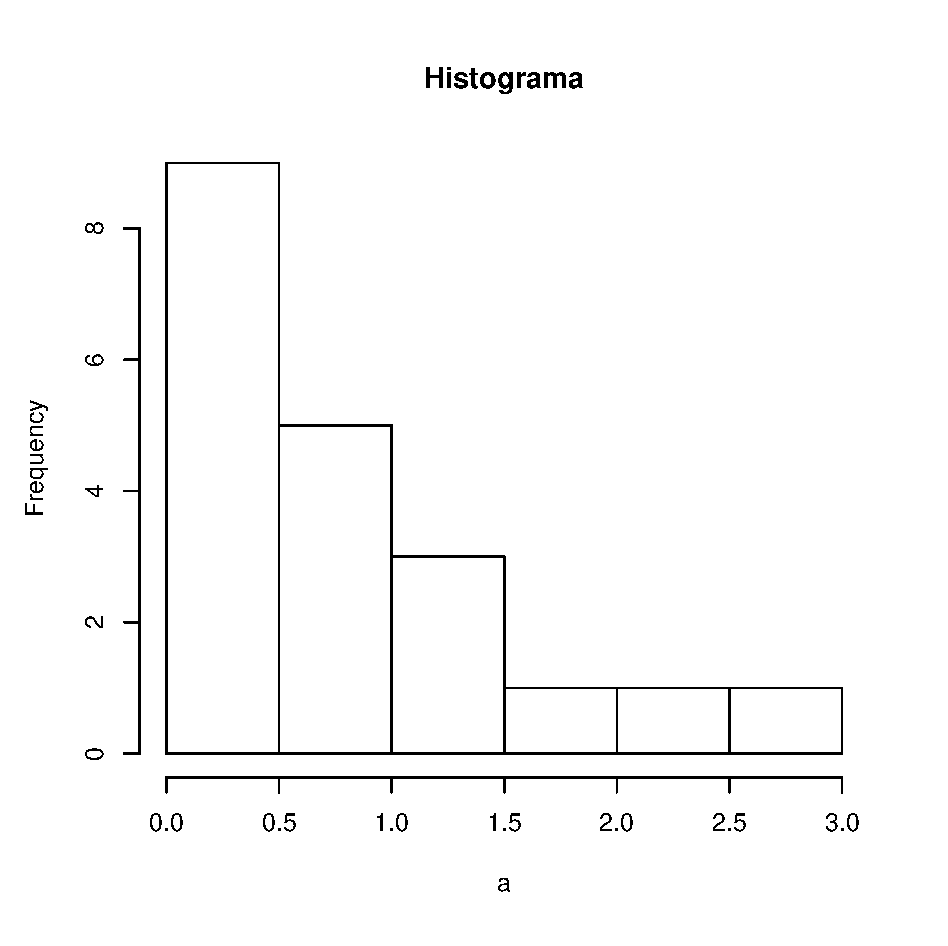
\includegraphics[scale=0.5]{Hist_ejemplo224.eps}
\caption{\textsl{Histograma de los datos del Ejemplo 2.3.4.}}
\end{figure}


\begin{figure}[!htb]
\centering
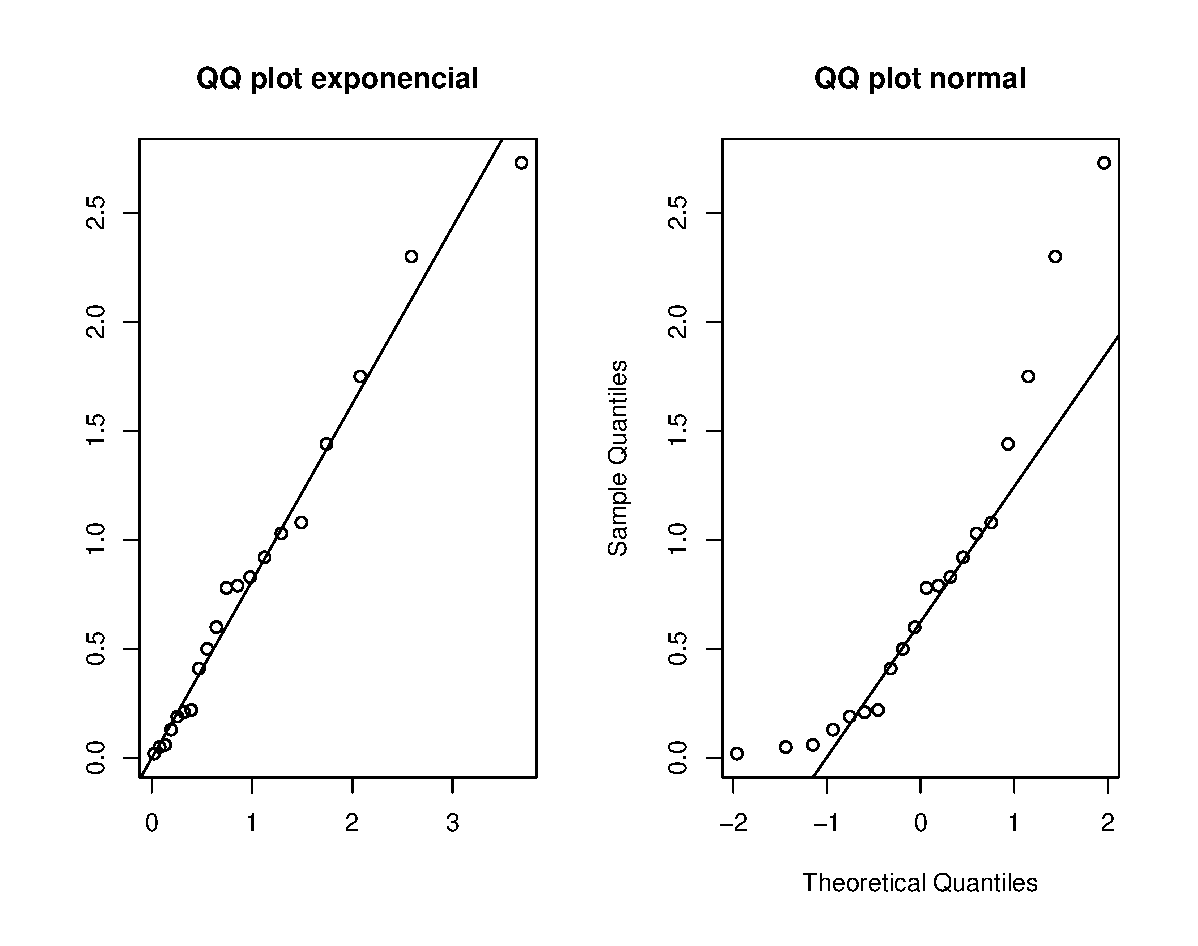
\includegraphics[scale=0.5]{Ejemplo2.2.4.eps}
\caption{\textsl{QQ plot para verificar la distribuci�n de los datos del Ejemplo 2.3.4.}}
\end{figure}

Ahora suponga que los directivos de la aerol�nea han observado que si un cliente tiene que esperar m�s de 2 minutos, con toda seguridad cuelga la llamada; el 30\% de los clientes que tienen que esperar entre 1 minuto y medio y 2 minutos cuelgan la llamada y ning�n cliente cuelga antes del minuto y medio. Entonces podemos estimar el porcentaje de clientes que cuelgan antes de ser atendidos, esto es, clientes potenciales que la aerol�nea pierde. Para eso, se debe estimar el porcentaje de llamadas que necesitan m�s de 2 minutos para ser atendidas, �ste se puede expresar como $Pr(X>2)$, donde $X$ denota el tiempo de espera de una llamada y $X\sim Exp(\theta)$. Entonces debe estimar $Pr(X>2)=e^{-2/\theta}$, la cual es una funci�n de $\theta$, y como ya se ha encontrado una estimaci�n de $\theta$ dada por $\hat{\theta}_{MV}=0.8$, podemos simplemente estimar $Pr(X>2)$ como $e^{-2/0.8}=0.08$, esto es, se estima que el 8\% de llamadas necesitan m�s de 2 minutos para ser atendidas, y por consiguiente este 8\% de clientes cuelga antes de ser atendido. Ahora, para estimar el porcentaje de llamadas que necesitan entre 1 minuto y medio y 2 minutos para ser atendidas como $e^{-1.5/0.8}-e^{-2/0.8}=0.07$, es decir, 7\% de llamadas requieren entre 1.5 y 2 minutos para ser atendidas, y por con\-si\-guien\-te $7\%\times 0.3=0.021=2.1\%$ de clientes cuelgan la llamada antes de ser atendida. Sumando el 8\% hallado anteriormente, podemos afirmar que se estima que la aerol�nea pierde el 10.1\% de los clientes potenciales por no ser atendidos oportunamente. M�s adelante, se ver� que esta estimaci�n sigue siendo de m�xima verosimilitud.
\end{Eje}

Las distribuciones consideradas anteriormente tienen s�lo un par�metro desconocido. Para distribuciones que tienen dos par�metros desconocidos, el procedimiento es levemente distinto, como lo ilustra el siguiente ejemplo con la distribuci�n normal.
\begin{Eje}
Dada una muestra aleatoria $X_1$, $\cdots$, $X_n$ con distribuci�n $N(\mu,\sigma^2)$\index{Estimador!de m�xima verosimilitud!normal}, el estimador de m�xima verosimilitud del vector de par�metros $\btheta=(\mu,\sigma^2)'$ es $(\bar{X},S_n^2)'$. Tenemos las siguientes expresiones para la funci�n de verosimilitud:
\begin{align*}
L(\btheta,x_1,\cdots,x_n)&=\frac{1}{\sqrt{\pi\sigma^2}}\exp\left\{-\frac{1}{2\sigma^2}(x_1-\mu)^2\right\}\cdots\frac{1}{\sqrt{\pi\sigma^2}}\exp\left\{-\frac{1}{2\sigma^2}(x_n-\mu)^2\right\}\\
                         &=(\pi\sigma^2)^{-n/2}\exp\left\{-\frac{1}{2\sigma^2}\sum_{i=1}^n(x_i-\mu)^2\right\}
\end{align*}
Para facilitar la maximizaci�n de $L$, se calcula $\ln(L)$:
\begin{equation*}
\ln(L)=-\frac{n}{2}\ln(\pi)-\frac{n}{2}\ln(\sigma^2)-\frac{1}{2\sigma^2}\sum_{i=1}^n(x_i-\mu)^2.
\end{equation*}

Ahora para obtener valores de $\mu$ y $\sigma^2$ que maximicen a $\ln(L)$, se procede a resolver las dos siguientes ecuaciones:

\begin{equation}\label{norm1}
\frac{\partial\ln(L)}{\partial\mu}=0\end{equation} y
\begin{equation}\label{norm2}\frac{\partial\ln(L)}{\partial\sigma^2}=0\end{equation}
Resolviendo la ecuaci�n (\ref{norm1}), se obtiene la soluci�n de $\mu=\bar{x}$ y resolviendo (\ref{norm2}), se obtiene la soluci�n de $\sigma^2=\sum(x_i-\mu)^2/n$, donde al reemplazar $\mu=\bar{x}$, se tiene que $\sigma^2=\sum(x_i-\bar{x})^2/n=s^2_n$.

Ahora debemos verificar que las anteriores soluciones halladas efectivamente ma\-xi\-mi\-cen la funci�n $\ln(L)$. Dado que esta funci�n tiene dos argumentos, es necesario hacer uso de la matriz Hessiana. La matriz se calcula de la siguiente manera:
\begin{align}\label{Hesiana_normal}
H(\ln(L))&=\begin{bmatrix}
\dfrac{\partial^2\ln(L)}{\partial\mu^2}&\dfrac{\partial^2\ln(L)}{\partial\mu\partial\sigma^2}\\
\dfrac{\partial^2\ln(L)}{\partial\sigma^2\partial\mu}&\dfrac{\partial^2\ln(L)}{\partial(\sigma^2)^2}
\end{bmatrix}\notag\\
&=\begin{bmatrix}
\dfrac{-n}{\sigma^2}&\dfrac{n\mu-\sum x_i}{\sigma^4}\\
\dfrac{n\mu-\sum x_i}{\sigma^4}&\dfrac{n}{2\sigma^4}-\dfrac{\sum(x_i-\mu)^2}{\sigma^6}
\end{bmatrix}.
\end{align}
Ahora reemplazamos las soluciones halladas $\mu=\bar{x}$ y $\sigma^2=s^2_n$, se tiene que la matriz Hessiana es:
\begin{equation*}
H=\begin{bmatrix}
\dfrac{-n^2}{\sum(x_i-\bar{x})^2}&0\\
0&\dfrac{-n^3}{2(\sum(x_i-\bar{x})^2)^2}
\end{bmatrix}.
\end{equation*}

Obs�rvese que la matriz Hessiana es una matriz diagonal con valores negativas en la diagonal, lo cual demuestra que es definida negativa, con eso se concluye que las soluciones halladas efectivamente maximizan la funci�n $\ln(L)$. En conclusi�n, los estimadores de m�xima verosimilitud del vector de par�metros $\btheta=(\mu,\sigma^2)'$ son $(\bar{X},S_n^2)'$.
\end{Eje}

A continuaci�n, se presenta una aplicaci�n del anterior ejemplo.

\begin{Eje}
Suponga que una f�brica de vidrios tiene una l�nea de producci�n de l�minas de vidrio templado de grosor de 3 cm. Para controlar la calidad de los vidrios producidos por esta l�nea, se seleccionan 12 l�minas para inspecci�n. Estas 12 l�minas midieron (en cm)  3.56, 3.36, 2.99, 2.71, 3.31, 3.68, 2.78, 2.95, 2.82, 3.45, 3.42 y 3.15. Estos datos son, aparentemente, continuos, y podemos pensar que una distribuci�n normal puede ser apropiada para los datos. Podemos, en primer lugar, observar la forma del histograma de estos datos presentando la Figura 2.3, donde aparentemente no se observa una forma similar a la funci�n de densidad de una distribuci�n normal.

\begin{figure}[!htb]
\centering
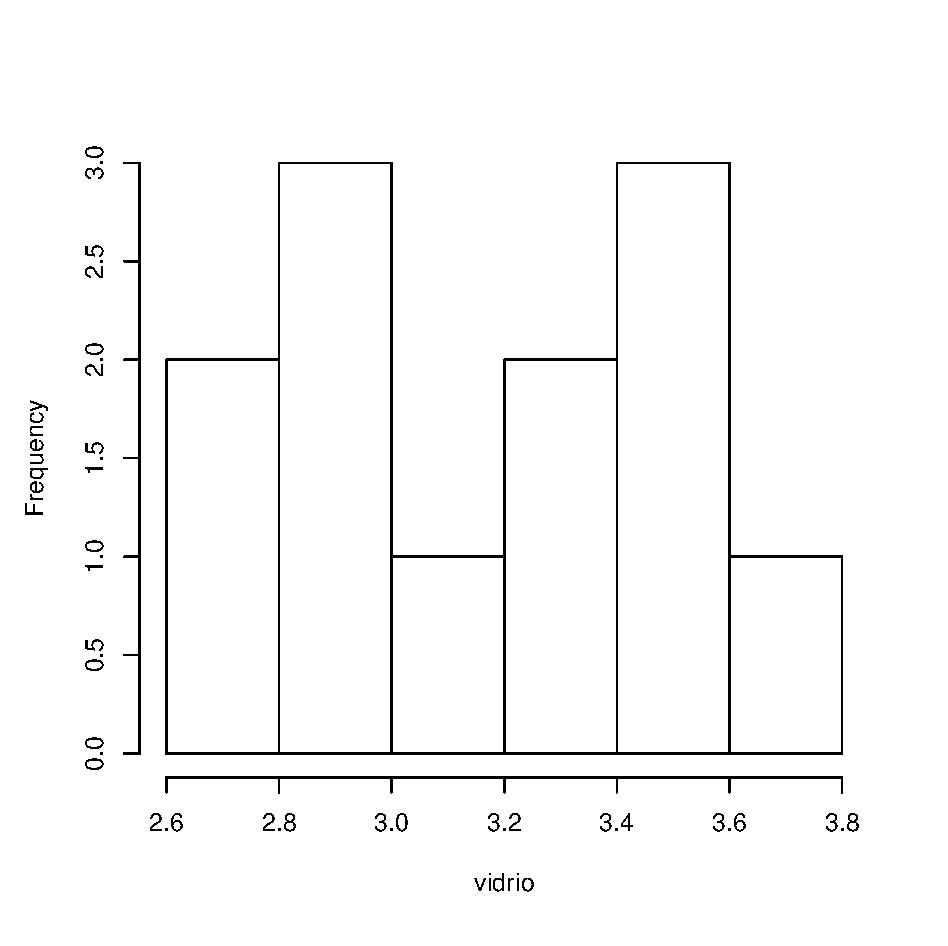
\includegraphics[scale=0.45]{histograma_vidrios.eps}
\caption{\textsl{Histograma de los datos del Ejemplo 2.3.6.}}
\end{figure}

Sin embargo, como el n�mero de datos es relativamente peque�o, el histograma puede no reflejar la distribuci�n verdadera de los datos, y por esta raz�n, usamos la gr�fica de QQ plot\index{Gr�ficas QQ plot!distribuci�n normal} para ver qu� tan adecuada es la distribuci�n normal. El comando en R est� dado a continuaci�n

\begin{verbatim}
    > vidrio<-c(3.56, 3.36, 2.99, 2.71, 3.31,3.68, 2.78, 2.95,
    2.82, 3.45, 3.42 ,3.15)
    > qqnorm(vidrio,main="QQ plot para distribuci�n normal",xlab=
    "Cuantiles teoricos",ylab="Cuantiles muestrales")
    > qqline(vidrio)
\end{verbatim}

Esta gr�fica se muestra en la Figura 2.4, donde podemos ver que una distribuci�n normal parece ser apropiada. Por lo tanto, usando el anterior ejemplo, podemos estimar el grosor promedio de las l�minas de esta l�nea como $\hat{\mu}_{MV}=\bar{x}=3.18\ cm$ y la varianza estimada en este caso es $\hat{\sigma}^2_{MV}=s^2_n=0.097\ cm^2$. Sin embargo, es dif�cil dar interpretaci�n pr�ctica a la varianza puesto que la unidad de �sta es la unidad de los datos al cuadrado, por esta raz�n en la pr�ctica se usa con m�s frencuencia $\sigma$ como la medida de dispersi�n. En este caso, tenemos que $\hat{\sigma}=\sqrt{0.097\ cm^2}=0.31\ cm$.

\begin{figure}[!htb]
\centering
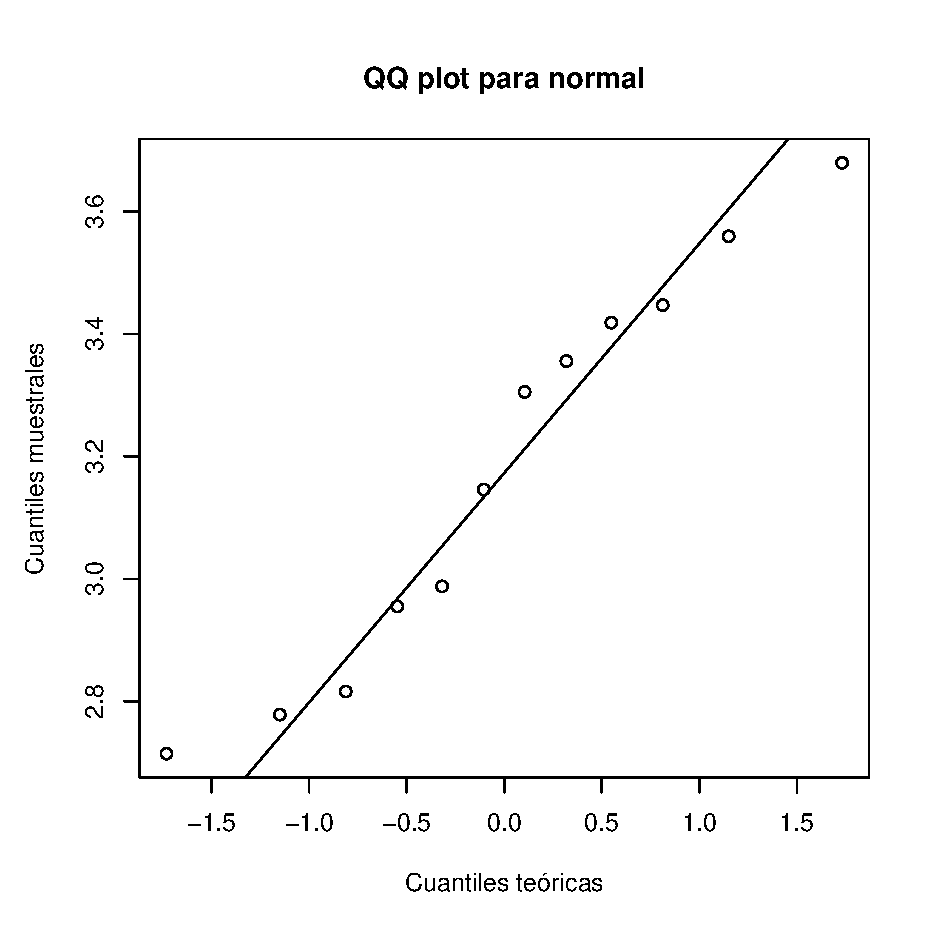
\includegraphics[scale=0.4]{qq_normal_ejemplo.eps}
\caption[\textsl{QQ plot para verificar la distribuci�n de los datos del Ejemplo 2.3.6}]{\textsl{QQ plot para verificar la distribuci�n normal de los datos del Ejemplo 2.3.6.}}
\end{figure}

Otra cantidad interesante que se quiere conocer es $\sigma/\mu$, que puede ser vista como una medida de dispersi�n te�rica que est� libre de las unidades de medici�n y por consiguiente, es �til en la pr�ctica para comparar dos poblaciones. Esta cantidad se puede ver como una funci�n del vector de par�metros $(\mu,\sigma^2)$, raz�n por la cual puede ser estimada por $\dfrac{\sqrt{S_n^2}}{\bar{X}}$ que en este ejemplo da como resultado 9.7\%.

Ahora, suponga que las l�minas de grosor entre 2.8 cm y 3.2 cm son vendidas al mercado, las de grosor menor de 2.8 cm son desechadas y las de grosor mayor de 3.2 son usadas como materia prima para futuras producciones. Usando las estimaciones de $\mu$ y $\sigma$ podemos estimar las proporciones de l�minas que ser�n vendidas, desechadas y usadas como materia prima. Si denotamos el grosor de una l�mina como $X$, tenemos que la proporci�n de l�minas que ser�n vendidas es igual a
\begin{align*}
Pr(2.8<X<3.2)&=Pr\left(\dfrac{2.8-\mu}{\sigma}<\dfrac{X-3.18}{0.31}<\dfrac{3.2-\mu}{\sigma}\right)\\
&=\Phi\left(\dfrac{3.2-\mu}{\sigma}\right)-\Phi\left(\dfrac{2.8-\mu}{\sigma}\right).
\end{align*}
Usando $\hat{\mu}_{MV}=3.18$ y $\hat{\sigma}=0.31$, podemos estimar la proporci�n de l�minas que ser�n vendidas como $\Phi\left(\dfrac{3.2-3.18}{0.31}\right)-\Phi\left(\dfrac{2.8-3.18}{0.31}\right)$, el cual es igual a 0.42. Es decir, se estima que s�lo el 42\% de las l�minas producidas ser�n vendidas.

An�logamente, se puede encontrar que el 11\% ser�n desechadas y el 47\% ser�n usadas como materia prima. Es claro que seg�n los datos muestrales y las estimaciones obtenidas de �stos, el uso de esta l�nea de producci�n no parece ser muy rentable, puesto que menos de la mitad de las l�minas producidas pueden ser vendidas. Para aumentar la proporci�n de l�minas que son aptas para la venta, la f�brica debe mejorar la l�nea de producci�n con la ayuda de los expertos para
\begin{itemize}
    \item Disminuir el grosor promedio de las l�minas, puesto que en la muestra se observ� un promedio de 3.18 cm, y se podr� pensar que el grosor real de las l�minas es superior al valor especificado de 3 cm. Suponga que despu�s de una mejora de la l�nea de producci�n, el promedio muestral fuera $\bar{x}=3.05$ y $\hat{\sigma}$ se mantiene igual. Se puede ver que en este caso, la proporci�n estimada de l�minas para venta se aumentar� a 48\%.
    \item Estabilizar las l�minas en t�rmino del grosor; de esta forma, la estimaci�n de $\sigma$ ser� m�s peque�a y la proporci�n de l�minas para venta se incrementar�. Suponga que despu�s de una mejora de la l�nea de producci�n, $\hat{\sigma}=0.2\ cm$ y $\hat{\mu}$ se mantiene igual. Se puede ver que la proporci�n estimada de l�minas para venta se aumentar� a 51\%.
\end{itemize}
Finalmente, si se puede lograr que $\mu$ sea m�s cercano a 3 cm y al mismo tiempo disminuir el valor de $\sigma$, la proporci�n de l�minas para venta ser� a�n mayor, y la l�nea de producci�n ser� m�s rentable.
\end{Eje}

En el anterior ejemplo, el estimador de m�xima verosimilitud de $\mu$ es $\bar{X}$, y esto es v�lido a�n cuando la varianza te�rica $\sigma^2$ es conocida; por otro lado, cuando $\mu$ es conocido, el estimador de m�xima verosimilitud de $\sigma^2$ ya no es $S^2_n$ sino $\sum_{i=1}^n(X_i-\mu)^2/n$, esto es, se mide la dispersi�n tomando las diferencia entre cada variable con la media te�rica $\mu$ (Ejercicio 2.5).

El problema de maximizar una funci�n puede, en algunos casos, resultar complicado, y peor a�n, puede no encontrar una soluci�n expl�cita. Un ejemplo de ello es la distribuci�n gamma cuando ambos par�metros son desconocidos. Para estos casos, es necesario usar m�todos num�ricos para encontrar el m�ximo de la funci�n de verosimilitud.

Ahora, para las distribuciones con dos par�metros como normal o gamma, cuando uno de los dos par�metros es fijo conocido, entonces s�lo habr� necesidad de estimar el otro par�metro y el procedimiento es similar al presentado anteriormente, y lo ilustramos en el siguiente ejemplo.

\begin{Eje}
Dada una muestra aleatoria $X_1$, $\cdots$, $X_n$ con distribuci�n Gamma\index{Estimador!de m�xima verosimilitud!Gamma} con par�metro de forma $k$ conocido y par�metro de escala $\theta$ desconocido, se tiene que el estimador de m�xima verosimilitud de $\theta$ es $\dfrac{\sum_{i=1}^nX_i}{nk}$. Para la verificaci�n, primero calculamos $\ln(L)$ que es la funci�n que se necesita maximizar:
\begin{align*}
\ln(L)&=\ln\left(\dfrac{\prod x_i^{k-1}e^{-\sum x_i/\theta}}{\theta^{nk}\Gamma(k)^n}\right)\\
      &=(k-1)\sum\ln(x_i)-\sum x_i/\theta-nk\ln\theta-n\ln(\Gamma(k))\\
\end{align*}
cuya primera derivada parcial con respecto a $\theta$ est� dada por:
\begin{equation*}
\frac{\partial\ln(L)}{\partial\theta}=\frac{\sum x_i}{\theta^2}-\frac{nk}{\theta},
\end{equation*}

el cual al igualar a 0, se obtiene la soluci�n de $\theta=\dfrac{\sum x_i}{nk}$. Ahora, al calcular la segunda derivada de $\ln(L)$ y evaluar en la anterior soluci�n, se tiene que
\begin{equation*}
\frac{\partial^2\ln(L)}{\partial\theta^2}=\frac{-nk}{\theta^2}<0,
\end{equation*}

con lo cual se concluye que el estimador de m�xima verosimilitud de $\theta$ es $\dfrac{\sum X_i}{nk}$.
\end{Eje}

Teniendo en cuenta que la distribuci�n exponencial es un caso particular de la distribuci�n Gamma cuando $k=1$, entonces del anterior ejemplo se puede concluir que el estimador de m�xima verosimilitud del par�metro $\theta$ de una distribuci�n exponencial es $\bar{X}=\dfrac{\sum X_i}{n}$, estimador que tambi�n se puede obtener maximizando directamente la funci�n de verosimilitud.

Cuando la funci�n de verosimilitud no es funci�n continua o derivable del par�metro $\theta$, el problema de maximizar no se puede llevar a cabo haciendo el uso de la derivada de la manera habitual, los dos siguientes ejemplos ilustran tales situaciones.

\begin{Eje}
\index{Estimador!de m�xima verosimilitud!hipergeom�trica}En situaciones donde la caracter�stica de inter�s es el tama�o de una poblaci�n $N$, puede ser, por ejemplo, la cantidad de cierto tipo de animales en un determinado lugar (puede ser un bosque). Una forma de determinar $N$ es, en primer lugar, identificar $R$ de los $N$ individuos ($R<N$); en el caso de los animales, puede ser conveniente capturar $R$ de ellos y marcarlos de alguna forma. Despu�s de eso, se espera que los $R$ individuos se mezclen bien con los otros $N-R$, y se seleccionan aleatoriamente $n$ individuos ($n<N$), y se cuenta cu�ntos de los $R$ individuos fueron seleccionados. Para ver c�mo este procedimiento nos puede ayudar a encontrar el valor de $N$, primero identifiquemos el contexto en t�rminos de las distribuciones probabil�sticas.

Sea $X$ la variable aleatoria que denota el n�mero de los $R$ individuos que fueron seleccionados en la muestra de tama�o $n$, entonces podemos ver que $X\sim Hg(n,R,N)$, donde $n$ y $R$ son conocidos, y se quiere encontrar el estimador de m�xima verosimilitud de $N$. En este caso la funci�n de verosimilitud es la misma funci�n de densidad de la variable $X$, esto es:
\begin{equation}\label{L_hipergeo}
L(N,x)=\frac{\binom{R}{x}\binom{N-R}{n-x}}{\binom{N}{n}}I_{\{0,1,\cdots,n\}}(x).
\end{equation}

En esta funci�n, el argumento $N$ toma valores discretos y no se puede derivar $L$ con respecto a $N$ para hallar el m�ximo. La forma de encontrar el valor de $N$ que maximiza a $L$ es encontrar para qu� valores de $N$, la funci�n $L$ es creciente y para qu� valores de $N$ es decreciente. Para lograr este fin, se despeja el valor de $N$ en $L(N)/L(N-1)>1$, como sigue:
\begin{equation*}
\begin{gathered}
\dfrac{L(N)}{L(N-1)}=\dfrac{\binom{N-R}{n-x}\binom{N-1}{n}}{\binom{N}{n}\binom{N-R-1}{n-x}}>1\\
\dfrac{(N-R)!(N-1)!(N-n)!(N-R-1-n+x)!}{(N-R-1)!N!(N-n-1)!(N-R-n+x)!}>1\\
(N-R)(N-n)>N(N-R-n+x)\\
Rn/x>N.\\
\end{gathered}
\end{equation*}
An�logamente, se obtiene que $L(N)/L(N-1)<1$ cuando $N>Rn/x$. Lo anterior indica que la funci�n $L$ es creciente para valores de $N$ menores que $Rn/x$ y decreciente para valores mayores que $Rn/x$. Pero no podemos afirmar que $Rn/X$ es el estimador de m�xima verosimilitud para $L$ puesto que este cociente puede no ser entero, y en este caso la estimaci�n no se ubicar�a dentro del espacio param�trico de $N$. Lo que s� se puede afirmar es que el estimador de m�xima verosimilitud de $N$ es $[Rn/X]$ o $[Rn/X]+1$ donde $[\cdot]$ es la funci�n parte entera. Shao (2003) afirma que $\hat{N}_{MV}=[Rn/X]$. Esto es verdadero, puesto que hemos encontrado anteriormente que $L(N)<L(N-1)$ si $N>Rn/x$, entonces podemos concluir que como $[Rn/x]+1>Rn/x$, entonces $L([Rn/x]+1)<L([Rn/x])$. Y podemos afirmar que el estimador de m�xima verosimilitud de $N$ es $[Rn/X]$.

Otra aplicaci�n interesante de la distribuci�n hipergeom�trica es el caso donde se conoce el tama�o poblacional $N$, y se desea estimar el n�mero de individuos que tienen cierta caracter�stica basada en una muestra de tama�o $n$; por ejemplo, se conoce que en un estanque hay $N$ peces, y se sabe que una parte de ellos est�n infectados por un tipo de par�sito, y se quiere saber cu�ntos peces tienen dicho par�sito con base en la observaci�n de una muestra de tama�o $n$. En estos casos, estamos interesados en estimar $R$ con $N$ y $n$ conocidos. Un razonamiento an�logo al caso de estimar $N$ conduce al siguiente estimador de $R$ \footnote{Para m�s detalles, consulte \citeasnoun{Zhang1}.}.
\begin{equation*}
\hat{R}_{MV}=\begin{cases}
\dfrac{x(N+1)}{n}-1\ \text{�}\ \dfrac{x(N+1)}{n}\ \ \ \ \ \ \text{si $\dfrac{x(N+1)}{n}$ es entero}\\
[\dfrac{x(N+1)}{n}]\ \ \ \ \ \ \ \ \ \ \ \ \ \ \ \ \ \ \ \ \ \ \ \ \ \text{si $\dfrac{x(N+1)}{n}$ no es entero}
\end{cases}
\end{equation*}

Retomando el problema de estimar el tama�o de un subgrupo considerado en el Cap�tulo 1, donde se supone que en una ciudad existen 2396 empresas que pueden clasificar en empresas grandes, medianas o peque�as seg�n el n�mero de empleados, si en una muestra aleatoria simple sin reemplazos de tama�o 200 se encuentran 28 empresas grandes, para tener una estimaci�n del n�mero total de empresas grandes en la ciudad, calculamos en primer lugar $28*(2396+1)/200=335.58$. Este n�mero no es entero, de donde concluimos que la estimaci�n de m�xima verosimilitud del n�mero de empresas grandes en la ciudad es de 335.
\end{Eje}

Finalmente, consideramos las distribuciones donde los valores que toma la variable aleatoria $X$ depende del par�metro $\theta$; por ejemplo, las distribuciones del tipo uniforme. Para este tipo de distribuciones, el procedimiento para encontrar $\hat{\theta}_{MV}$ en general se puede resumir en los siguientes pasos:
\begin{enumerate}[(1)]
\item Calcular la funci�n de verosimilitud, sin omitir las funciones indicadoras, pues �stas dependen de $\theta$.
\item Encontrar el rango de valores de $\theta$ donde la funci�n de verosimilitud no toma el valor 0. Generalmente este rango depende del m�ximo y/o el m�nimo de la muestra: $x_{(n)}$ y $x_{(1)}$.
\item Dentro del rango encontrado en el paso anterior, mediante empleo de derivadas o simplemente observaci�n directa, buscar el valor de $\theta$ que maximice la funci�n de verosimilitud.
\end{enumerate}
Ilustramos el anterior procedimiento en el siguiente ejemplo.

\begin{Eje}
\index{Estimador!de m�xima verosimilitud!uniforme}Dada una muestra aleatoria $X_1$, $\cdots$, $X_n$ proveniente de una poblaci�n con distribuci�n uniforme continua sobre el intervalo $[0,\theta]$, se quiere encontrar el estimador de m�xima verosimilitud del par�metro $\theta$. En primer lugar, obs�rvese que en la funci�n de verosimilitud $L$ existe un t�rmino de la funci�n indicadora que depende de $\theta$, puesto que $L(\theta)=\theta^{-n}\prod_{i=1}^nI_{[0,\theta]}(x_i)$.

Tenemos que
\begin{equation*}
L\neq0\Leftrightarrow0\leq x_i\leq\theta\ \text{para todo } i=1,\cdots,n\ \Leftrightarrow \theta\geq x_{(n)}
\end{equation*}
donde $x_{(n)}=\max\{x_1,\cdots,x_n\}$. Entonces se concluye que el rango de valores de $\theta$ para que la funci�n de verosimilitud sea diferente de 0 es $[x_{(n)},\infty)$. Ahora, observe que dentro de este rango, $L=\theta^{-n}$, que es una funci�n decreciente de $\theta$, entonces para valores peque�os de $\theta$, $L$ toma valores grandes. Pero el valor m�s peque�o que puede tomar $\theta$ dentro del rango $[x_{(n)},\infty)$ es $x_{(n)}$, entonces se concluye que $\hat{\theta}_{MV}=X_{(n)}$.
\end{Eje}

Ahora, retomando situaciones donde la cantidad que se quiere estimar es una funci�n del par�metro, $g(\theta)$, textos como \citeasnoun{Mood} establecen que el estimador de m�xima verosimilitud de $g(\theta)$ es simplemente $g(\hat{\theta}_{MV})$ siempre y cuando $g$ es una funci�n uno a uno.

Otra forma de ver esto es mediante la reparametrizaci�n de la funci�n $L(\theta)$. Por ejemplo, suponga que se desea estimar $\lambda=e^{-\theta}$ en una muestra proveniente de una distribuci�n $Pois(\theta)$. Podemos escribir la funci�n de verosimilitud en t�rmino de $\lambda$ como
\begin{equation*}
L(\lambda)=\dfrac{\lambda^n(-n\ln\lambda)^{\sum_{i=1}^nx_i}}{\prod_{i=1}^nx_i}\prod_{i=1}^nI_{\{0,1,\cdots\}}(x_i),
\end{equation*}

de donde
\begin{equation*}
\frac{\partial\ln L(\lambda)}{\partial\lambda}=\frac{n}{\lambda}+\frac{\sum_{i=1}^nx_i}{\ln\lambda}\frac{1}{\lambda},
\end{equation*}

igualando la anterior expresi�n a 0 y resolviendo para $\lambda$, se tiene que $\hat{\lambda}_{MV}=e^{-\bar{X}}$. Ahora, recordando que $\hat{\theta}_{MV}=\bar{X}$, lo cual coincide con la conclusi�n dada anteriormente.

Aunque lo planteado es v�lido para el caso cuando la funci�n $g$ es una funci�n uno a uno, existe el siguiente resultado que establece la invarianza del estimador de m�xima verosimilitud\index{Estimador!de m�xima verosimilitud!invarianza} para cualquier funci�n $g$.
\begin{Res}
Dada una muestra aleatoria $X_1$, $\cdots$, $X_n$ proveniente de una po\-bla\-ci�n con distribuci�n $f(x,\btheta)$ donde $\btheta$ es el vector de par�metros, y suponga que $T=T(X_1,\cdots,X_n)$ es el estimador de m�xima verosimilitud de $\btheta$, y $g$ es una funci�n del vector de par�metros, entonces el estimador de m�xima verosimilitud de $g(\btheta)$ es la estad�stica $g(T)$.
\end{Res}
\begin{proof}
\citeasnoun[p. 172 y p. 321]{Casella}.
\end{proof}

Dado el anterior resultado, podemos ver que todas las estimaciones de los Ejemplos 2.3.2, 2.3.3, 2.3.4 y 2.3.6 son estimaciones de m�xima verosimilitud.

Otra situaci�n interesante es cuando se dispone de dos muestras aleatorias independientes, esto es, cualquier conjunto de variables de la primera muestra es independiente de cualquier conjunto de variables de la segunda, y el objetivo es estimar los par�metros concernientes a las dos muestras.

Consideramos, en primer lugar, dos muestras provenientes de distribuciones normales.

\index{Estimador!de m�xima verosimilitud!normal!dos muestras}Suponga que se tienen dos muestras aleatorias independientes $X_1$, $\ldots$, $X_{n_X}$ y $Y_1$, $\ldots$, $Y_{N_Y}$ provenientes de $N(\mu_X,\sigma^2_{X})$ y $N(\mu_Y,\sigma^2_Y)$, respectivamente. Y se desean estimar algunos de los par�metros $\mu_X$, $\mu_Y$, $\sigma^2_X$ y $\sigma^2_Y$. En primer lugar, calculamos la funci�n de verosimilitud, la cual est� dada por
\begin{equation*}
L=(2\pi\sigma^2_X)^{-n_X/2}(2\pi\sigma^2_Y)^{-n_Y/2}\exp\left\{-\frac{1}{2\sigma^2_X}\sum_{i=1}^{n_X}(x_i-\mu_X)^2-\frac{1}{2\sigma^2_Y}\sum_{j=1}^{n_Y}(y_j-\mu_Y)^2\right\}
\end{equation*}

En el caso de que las dos muestras provenientes de la misma distribuci�n, esto es, si $\mu_X=\mu_Y=\mu$ y $\sigma^2_X=\sigma^2_Y=\sigma^2$, entonces el proceso de la estimaci�n de m�xima verosimilitud de $\mu$ y $\sigma^2$ se llevan a cabo, simplemente, usando conjuntamente las variables de las dos muestras. Y tenemos que
\begin{equation}\label{MV_mu_comun1}
\hat{\mu}_{MV}=\dfrac{\sum_{i=1}^{n_X}X_i+\sum_{j=1}^{n_Y}Y_j}{n_X+n_Y},
\end{equation}
y
\begin{equation*}
\hat{\sigma}^2_{MV}=\dfrac{\sum_{i=1}^{n_X}(X_i-\hat{\mu}_{MV})^2+\sum_{j=1}^{n_Y}(Y_j-\hat{\mu}_{MV})^2}{n_X+n_Y}.
\end{equation*}
\begin{Eje}
Retomamos el Ejemplo 2.3.6, donde se dispon�a una muestra de 12 l�minas. Ahora suponga que se selecciona una nueva muestra de 10 l�minas de la misma l�nea de producci�n con grosor 3.56, 3.17, 2.98, 2.95, 3.03, 2.87, 3.58, 3.73, 2.83 y 3.43. Dado que las dos muestras son productos de una misma l�nea de producci�n, entonces podemos afirmar que las dos muestras provienen de una misma distribuci�n normal $N(\mu,\sigma^2)$, y podemos estimar el grosor promedio de esta l�nea como 3.2 cm y la desviaci�n est�ndar como 0.31 cm.
\end{Eje}

\index{Estimador!de m�xima verosimilitud!normal!dos muestras}Otra situaci�n que puede surgir en la pr�ctica es cuando las dos muestras provienen de distribuciones con la misma esperanza, pero diferentes varianzas, esto es, $\mu_X=\mu_Y=\mu$ y $\sigma^2_X\neq\sigma^2_Y$. Supongamos, en primer lugar, que $\sigma^2_X$ y $\sigma^2_Y$ son conocidas, y tenemos que la funci�n de verosimilitud est� dada por
\begin{equation*}
L(\mu)=(2\pi\sigma^2_X)^{-n_X/2}(2\pi\sigma^2_Y)^{-n_Y/2}\exp\left\{-\frac{1}{2\sigma^2_X}\sum_{i=1}^{n_X}(x_i-\mu)^2-\frac{1}{2\sigma^2_Y}\sum_{j=1}^{n_Y}(y_j-\mu)^2\right\}
\end{equation*}
de donde
\begin{equation*}
\dfrac{\partial\ln L(\mu)}{\partial\mu}=\frac{\sum_{i=1}^{n_X}(x_i-\mu)}{\sigma^2_X}+\frac{\sum_{j=1}^{n_Y}(y_j-\mu)}{\sigma^2_Y}.
\end{equation*}
Igualando la anterior derivada a cero y despejando $\mu$, se encuentra que la soluci�n est� dada por
$\mu=\dfrac{\sigma^2_Yn_X\bar{x}+\sigma^2_Xn_Y\bar{y}}{n_X\sigma^2_Y+n_Y\sigma^2_X}$. Ahora, es claro que
\begin{equation*}
\dfrac{\partial^2\ln L(\mu)}{\partial\mu^2}=-\dfrac{n_X}{\sigma^2_X}-\frac{n_Y}{\sigma^2_Y}<0,
\end{equation*}

y en conclusi�n, se tiene que
\begin{align}\label{MV_mu_comun}
\hat{\mu}_{MV}&=\dfrac{\sigma^2_Yn_X\bar{X}+\sigma^2_Xn_Y\bar{Y}}{n_X\sigma^2_Y+n_Y\sigma^2_X}\notag\\
&=\dfrac{n_X\bar{X}+n_Y\bar{Y}\frac{\sigma^2_X}{\sigma^2_Y}}{n_X+n_Y\frac{\sigma^2_X}{\sigma^2_Y}}.
\end{align}
N�tese que la anterior expresi�n se asemeja a un promedio ponderado, donde entre m�s grande sea la varianza te�rica de la segunda poblaci�n $\sigma^2_Y$, menos peso tienen las variables de la muestra correspondiente. Esto es muy natural, puesto que en una distribuci�n normal, una varianza grande indica que los valores de la distribuci�n tienden a tomar valores muy alejados a la media. Entonces, si $\sigma^2_X/\sigma^2_Y<1$, los valores de las variables $Y_1$, $\cdots$, $Y_{n_Y}$ tienden a estar m�s lejos de $\mu$ que las variables $X_1$, $\cdots$, $X_{n_X}$, lo cual las hacen menos confiables, y por esta raz�n se les asigna un peso menor. Cuando $\sigma^2_X=\sigma^2_Y$, la anterior estimaci�n de $\mu$ se reduce a (\ref{MV_mu_comun1}).

\begin{Eje}
Considera la f�brica vidrios del Ejemplo 2.3.6, y suponga que hay, en total, dos l�neas de producci�n de l�minas de vidrio templado de 3 cm, y adem�s por ajuste inapropiado de temperatura, la l�nea A tiene una desviaci�n est�ndar del 0.6 cm, mucho mayor que la l�nea B cuya desviaci�n est�ndar es del 0.3 cm. Si se desea estimar el grosor promedio de las l�minas de vidrio del grosor nominal del 3 cm, se debe seleccionar una muestra de las l�minas de la l�nea A, y una muestra de la l�nea B. Suponga que el grosor de 10 l�minas de cada l�nea corresponde a 3.80, 2.81, 2.98, 2.97, 3.69, 2.77, 3.08, 2.98, 2.37, 3.00 y 2.87, 3.48, 2.65, 3.38, 2.75, 2.99, 2.81, 2.54, 2.84, 2.79, respectivamente, entonces asignando un peso mayor a las observaciones de la l�nea B seg�n la teor�a expuesta anteriormente, se tiene que $\hat{\mu}_{MV}=2.955$ cm.
\end{Eje}

\index{Estimador!de m�xima verosimilitud!normal!dos muestras}Finalmente, consideramos el caso donde se supone que las dos varianzas te�ricas coinciden, $\sigma^2_X=\sigma^2_Y=\sigma^2$ y $\mu_X\neq\mu_Y$. En este caso, tenemos que los estimadores de m�xima verosimilitud de $\mu_X$, $\mu_Y$ y $\sigma^2$ son $\bar{X}$, $\bar{Y}$ y $[\sum_{i=1}^{n_X}(X_i-\bar{X})^2+\sum_{j=1}^{n_Y}(Y_j-\bar{Y})^2]/(n_X+n_Y)$, respectivamente (Ejercicio 2.25), esto es, las observaciones de las dos muestras se utilizan separadamente para estimar las medias te�ricas, mientras que la varianza se estima usando las muestras conjuntamente con la misma ponderaci�n. En general, cuando no se puede asumir que $\sigma^2_X=\sigma^2_Y$, los estimadores de m�xima verosimilitud de $\mu_X$ y $\mu_Y$ siguen siendo $\bar{X}$ y $\bar{Y}$, respectivamente.

\begin{Eje}
Suponga que se desea comparar dos institutos de capacitaci�n en t�rmino de calificaci�n obtenida por sus respectivos alumnos. Las calificaciones (sobre 100 puntos) para 15 alumnos del centro A es: 75, 87, 83, 73, 74, 88, 88, 74, 64, 92, 73, 87, 91, 83 y 84; y para 13 alumnos del centro B es: 64, 85, 72, 64, 74, 93, 70, 79, 79, 75, 66, 83 y 74. Antes de entrar a a analizar los datos, consideremos una distribuci�n que puede ser apropiada para estos datos. Dada la naturaleza del problema, los datos son enteros entre 0 y 100, y por consiguiente debe ser realizaci�n de una variable discreta; sin embargo, a veces, una distribuci�n continua tambi�n puede ser apropiada para describir datos discretos. En la Figura 2.5, se muestran las gr�ficas QQ plot de la distribuci�n normal para estos dos conjuntos de datos, donde podemos ver que la distribuci�n normal puede ser apropiada para estos datos.

\begin{figure}[!htb]
\centering
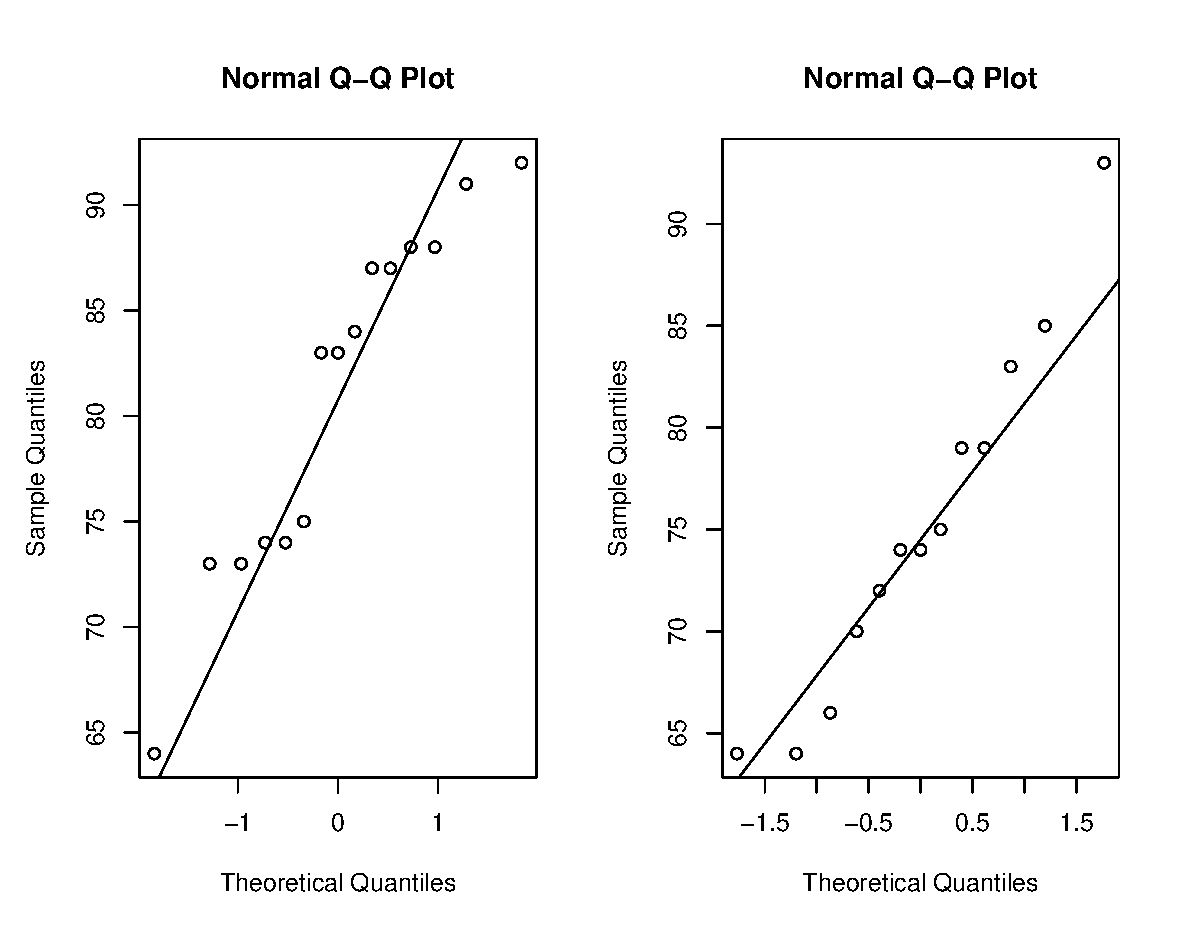
\includegraphics[scale=0.6]{Ejemplo_normal_2_muestra.eps}
\caption{\textsl{Gr�ficas de QQ plot para los datos del Ejemplo 2.3.12.}}
\end{figure}

Ahora, dado que el objetivo es comparar los dos institutos, no se puede asumir la igualdad entre las dos medias te�ricas; de esta forma, las dos medias te�ricas se estiman mediante las medias muestrales dadas por $\hat{\mu}_A=81$ y $\hat{\mu}_B=75$. Observamos que la estimaci�n para el media te�rica del centro A es superior a la del centro B. En los cap�tulos 3 y 4 se estudiar�n herramientas que nos permiten concluir si esta diferencia es significativa o puede considerarse como insignificante, dado que las estimaciones no se pueden tratar como si fueran los valores verdaderos de los par�metros.
\end{Eje}

En algunas situaciones, se desea comparar dos poblaciones en t�rmino de la dispersi�n tal como lo muestra el siguiente ejemplo.

\begin{Eje}
Suponga que se desea estudiar el precio por metro cuadrado de viviendas en el centro de la capital de los pa�ses Colombia y Ecuador. La informaci�n disponible para el caso de Colombia basada en 80 viviendas es: $\bar{x}=700$ (miles de pesos colombianos) y $s_{x,n}=95$ (miles de pesos colombianos); y para el caso ecuatoriano basado en 50 viviendas es: $\bar{y}=1023$ (bol�vares venezolanos) y $s_{y,m}=300$ (bol�vares venezolanos).

Dados los anteriores datos, no se puede comparar la dispersi�n de los dos pa�ses usando directamente las desviaciones est�ndares, puesto que �stas tienen unidades diferentes. Una alternativa es calcular los respectivos coeficientes de variaci�n dados por $\rho_x=95/700=13.57\%$ y $\rho_y=300/1023=29.32\%$. Estos coeficientes de variaci�n est�n libres de unidad de los datos originales y pueden ser usados directamente para comparar la dispersi�n. Y podemos concluir que el precio de la vivienda del centro del capital de pa�s vecino es mucho m�s inestable que en el caso colombiano.
\end{Eje}

\subsection{M�todo de los momentos\index{M�todo de los momentos}}
Otro m�todo com�n para encontrar estimadores de un par�metro es el m�todo de los momentos. Para estudiar este m�todo, primero introducimos algunas definiciones �tiles.
\begin{Defi}
Dada una variable aleatoria $X$, se define el $k$-�simo momento\index{Momento} de $X$ como $\mu_k=E(X^k)$.
\end{Defi}

La anterior definici�n es al nivel poblacional. Cuando se dispone de una muestra aleatoria, se definen los momentos muestrales como sigue.
\begin{Defi}
Dada una muestra aleatoria $X_1$, $\cdots$, $X_n$, se define el $k$-�simo momento muestral\index{Momento muestral} como $M_k=\sum_{i=1}^nX_i^k/n$.
\end{Defi}
N�tese que dada una muestra aleatoria, los momentos muestrales son variables aleatorias; m�s aun, son estad�sticas. Y podemos utilizarlos para estimar los respectivos momentos te�ricos. Ahora, si logramos escribir a los par�metros desconocidos en t�rminos de los momentos te�ricos, podemos obtener f�cilmente estimadores de los par�metros simplemente reemplazando los momentos te�ricos por los muestrales. Los estimadores obtenidos de esta manera se llaman estimadores de momentos\index{Estimador!de momentos}, se denotar� por $\hat{\theta}_{mom}$. En particular, tenemos el siguiente resultado que es v�lido en muestras provenientes de cualquier distribuci�n.

\begin{Res}
Dada una muestra aleatoria $X_1$, $\cdots$, $X_n$ con esperanza com�n $\mu$ y varianza com�n $\sigma^2$, se tiene que $\hat{\mu}_{mom}=\bar{X}$ y $\hat{\sigma^2}_{mom}=S^2_n$.\index{Estimador!de momentos!media te�rica}\index{Estimador!de momentos!varianza te�rica}
\end{Res}
\begin{proof}
En primer lugar, n�tese que la esperanza $\mu$ es simplemente el primer momento te�rico, es decir, $\mu=\mu_1$, el cual se estima con el primer momento muestral $M_1$, entonces se tiene que $\hat{\mu}_{mom}=M_1=\bar{X}$.

Ahora, la varianza te�rica $\sigma^2$ se puede escribir en t�rminos de los dos primeros momentos te�ricos, $\sigma^2=\mu_2-(\mu_1)^2$, que se estimar� con $M_2-(M_1)^2$, esto es: $\frac{1}{n}\sum_{i=1}^nX_i^2-\bar{X}^2$, y con un poco de operaci�n algebraica, se puede ver que �sta es $S^2_n=\frac{1}{n}\sum_{i=1}^nX_i^2-\bar{X}^2$. En conclusi�n, $\hat{\sigma^2}_{mom}=S^2_n$.
\end{proof}

Una aplicaci�n inmediata del anterior resultado es en una muestra proveniente de una distribuci�n normal donde los par�metros $\mu$ y $\sigma^2$ corresponden a la esperanza y la varianza de la distribuci�n.
\begin{Eje}
Dada una muestra aleatoria $X_1$, $\cdots$, $X_n$ proveniente de una distribuci�n $N(\mu,\sigma^2)$, el estimador de momentos de $\mu$ y $\sigma^2$ es simplemente la media y la varianza muestral: $\bar{X}$ y $S^2_n=\sum(X_i-\bar{X})^2/n$. N�tese que en este caso, los estimadores de momentos coinciden con los de m�xima verosimilitud.\index{Estimador!de momentos!normal}
\end{Eje}

Otra utilidad del Resultado 2.3.2 es la siguiente forma para encontrar un estimador de momentos.
\begin{enumerate}[(a)]
\item Cuando hay que estimar un s�lo par�metro $\theta$, escribir a $\theta$ en t�rmino de la media te�rica $\mu$: $\theta=g(\mu)$, y al estimar $\mu$ con la media muestral: $\bar{X}$, se obtiene un estimador de momentos para $\theta$. Esto es, $\hat{\theta}_{mom}=g(M_1)$.\footnote{Este m�todo es v�lido siempre y cuando se pueda escribir al par�metro en t�rmino de la media te�rica. En casos donde esto no es posible, por ejemplo en distribuciones donde no existe la media te�rica o �sta no depende del par�metro, se debe recurrir a momentos te�ricos superiores.} (tambi�n se puede escribir $\theta$ en t�rmino de la varianza te�rica $\sigma^2$, y al estimar $\sigma^2$ con $S^2_n$, se tiene un estimador de momentos de $\theta$).
\item Cuando hay que estimar dos par�metros $\theta_1$ y $\theta_2$, escribir a cada uno de ellos en t�rmino de la media y la varianza te�rica $\theta_1=g_1(\mu,\sigma^2)$ y $\theta_2=g_2(\mu,\sigma^2)$, y al estimar $\mu$ y $\sigma^2$ con la media muestral $\bar{X}$ y la varianza muestral $S^2_n$, se obtiene un estimador de momentos para $\theta_1$ y $\theta_2$. Esto es, $\hat{\theta}_{1,mom}=g_1(\bar{X},S^2_n)$ y $\hat{\theta}_{2,mom}=g_2(\bar{X},S^2_n)$.
\end{enumerate}

\textbf{Nota}: la parte (a) nos ilustra que el estimador de momentos al igual que el estimador de m�xima verosimilitud, puede no ser �nico. Un ejemplo es cuando la muestra aleatoria proviene de la distribuci�n $Pois(\lambda)$, se sabe que $\lambda=E(X)$, entonces un estimador de momentos de $\lambda$ es, naturalmente, $\bar{X}$. Pero tambi�n se sabe que $\lambda=Var(X)$; de esta manera, se tiene otro estimador de $\lambda$ que es $S^2_n$.\index{Estimador!de momentos!Poisson}

De esta forma, para los datos del Ejemplo 2.3.2, podemos tener dos estimaciones de momentos para el n�mero promedio de muertes violentas por ciudad: $\bar{x}=3.13$, la cual coincide con la estimaci�n de m�xima verosimilitud; y la otra estimaci�n de momentos corresponde a $s^2_n=1.98$, que es muy diferente a la estimaci�n obtenida usando $\bar{x}$. La pregunta natural ahora es �cu�l de las dos estimaciones es mejor?, es decir, �cu�l valor se acerca m�s al valor verdadero de $\lambda$? No podemos responder esta pregunta directamente, puesto que no conocemos el valor de $\lambda$. En la siguiente secci�n, se introducen conceptos que nos permiten evaluar la calidad de los estimadores. A pesar de que hasta ahora no tenemos herramientas para escoger entre las dos estimaciones, un simple ejercicio de simulaci�n nos permite escoger de forma emp�rica. Se simula, en primer lugar, muestras provenientes de una distribuci�n $Pois(5)$ y $Pois(15)$ con tama�o de muestra $n=5,\cdots,300$, y en cada muestra simulada, se calculan las dos estimaciones de momentos $\bar{x}$ y $s^2_n$, y se observa cu�l es m�s cercano al valor verdadero del par�metro. Los resultados se visualizan en la gr�fica superior de la Figura 2.6, donde la l�nea negra horizontal denota el valor verdadero del par�metro $\lambda$. El comando en R de estas simulaciones es como sigue

\begin{verbatim}
> set.seed(123)
> n<-5:300
> est.mean<-rep(NA,length(n))
> est.var<-rep(NA,length(n))
> for(i in 1:length(n)){
+ x<-rpois(n[i],5)
+ est.mean[i]<-mean(x)
+ est.var[i]<-var(x)*(n[i]-1)/n[i]
+ }
>
> est1.mean<-rep(NA,length(n))
> est1.var<-rep(NA,length(n))
> for(i in 1:length(n)){
+ y<-rpois(n[i],15)
+ est1.mean[i]<-mean(y)
+ est1.var[i]<-var(y)*(n[i]-1)/n[i]
+ }
>
>
> par(mfrow=c(2,1))
> plot(n,est.var,xlab="n",ylab="Estimaci�n",main="Poblaci�n P(5)",
type="l",col="blue",ylim=c(2,9))
> abline(5,0)
> lines(n,est.mean,col="red")
> legend(200,9.2,c("Media","Varianza"),lty=c(1,1),col=c("red","blue"),
+  box.col=0)
>
> plot(n,est1.var,xlab="n",ylab="Estimaci�n",main="Poblaci�n P(15)",
type="l",col="blue")
> abline(15,0)
> lines(n,est1.mean,col="red")
> legend(200,45,c("Media","Varianza"),lty=c(1,1),col=c("red","blue"),
+  box.col=0)
\end{verbatim}

Se puede ver claramente, de la Figura 2.6, que la media $\bar{X}$ comparada con $S^2_n$ estima mejor el par�metro de la distribuci�n, puesto que las estimaciones de $\bar{X}$ parecen estar m�s cercanas del valor de $\lambda$ en ambas gr�ficas. Y por consiguiente, podemos intuir que para los datos del Ejemplo 2.3.2, la estimaci�n $\bar{x}=3.13$ debe ser m�s cercana al valor verdadero de $\lambda$. En la siguiente secci�n, se discutir�n m�todos formales acerca de escogencia entre estimadores, y se ver� que el estimador $\bar{X}$ tiene mejores propiedades que $S^2_n$.

En los siguientes ejemplos, se ilustra la forma general de encontrar estimadores de momentos para distribuciones con dos par�metros desconocidos.

\begin{Eje}
Dada una muestra aleatoria $X_1$, $\cdots$, $X_n$ proveniente de una distribuci�n gamma\index{Estimador!de momentos!Gamma} con par�metro de forma $k$ y par�metro de escala $\theta$, entonces la media y la varianza te�rica est�n dadas por $\mu=k\theta$ y $\sigma^2=k\theta^2$, de donde podemos expresar $k$ y $\theta$ en t�rmino de $\mu$ y $\sigma^2$ como $k=\frac{\mu^2}{\sigma^2}$ y $\theta=\frac{\sigma^2}{\mu}$. Por lo tanto, los estimadores de momentos ser�n
\begin{equation}\label{k_gamma}
\hat{k}_{mom}=\dfrac{\bar{X}^2}{S^2_n}
\end{equation}

y
\begin{equation}\label{theta_gamma}
\hat{\theta}_{mom}=\dfrac{S^2_n}{\bar{X}}
\end{equation}
.

\begin{figure}[!h]
\centering
\includegraphics[scale=0.7]{estimadores_Poisson.eps}
\caption[\textsl{Media y la varianza muestral como estimador de $\lambda$ en Poisson}]{\textsl{Comparaci�n entre la media y la varianza muestral como estimador de $\lambda$ en muestras provenientes de dos distribuciones Poisson.}}
\end{figure}

Como una aplicaci�n de lo anterior, suponga que un instituto t�cnico enfrenta problemas financieros y plantea un aumento en el costo de las matr�culas. Es claro que ante un aumento del valor de matr�cula, los estudiantes que no tengan la capacidad de pago pueden retirarse del instituto, lo que representa una p�rdida econ�mica para �ste. Por lo anterior es necesario que el instituto conozca el nivel de ingreso de los estudiantes con el fin de decidir sobre el aumento de las matr�culas que no cause la deserci�n estudiantil y a la vez pueda representar una ganancia econ�mica para el instituto.

Con el fin de conocer el nivel de ingreso de los estudiantes, el instituto plane� una encuesta donde 127 estudiantes del instituto suministraron el valor de sus ingresos mensuales. Es usual pensar que una distribuci�n Gamma puede ser apropiada para variables como ingreso puesto que en primer lugar, esta variable toma valores positivos, y en segundo lugar, es altamente no sim�trica, ya que para la mayor�a de la poblaci�n la variable ingreso toma valores intermedios o bajos, pero existe una minor�a de la poblaci�n que tiene ingresos bastantes altos. Para observar el comportamiento del ingreso en los 127 datos muestrales, observamos el histograma presentado en la Figura 2.7, donde se puede ver estas caracter�sticas reflejas, y finalmente asumimos la distribuci�n Gamma como la distribuci�n te�rica.

\begin{figure}[!htb]
\centering
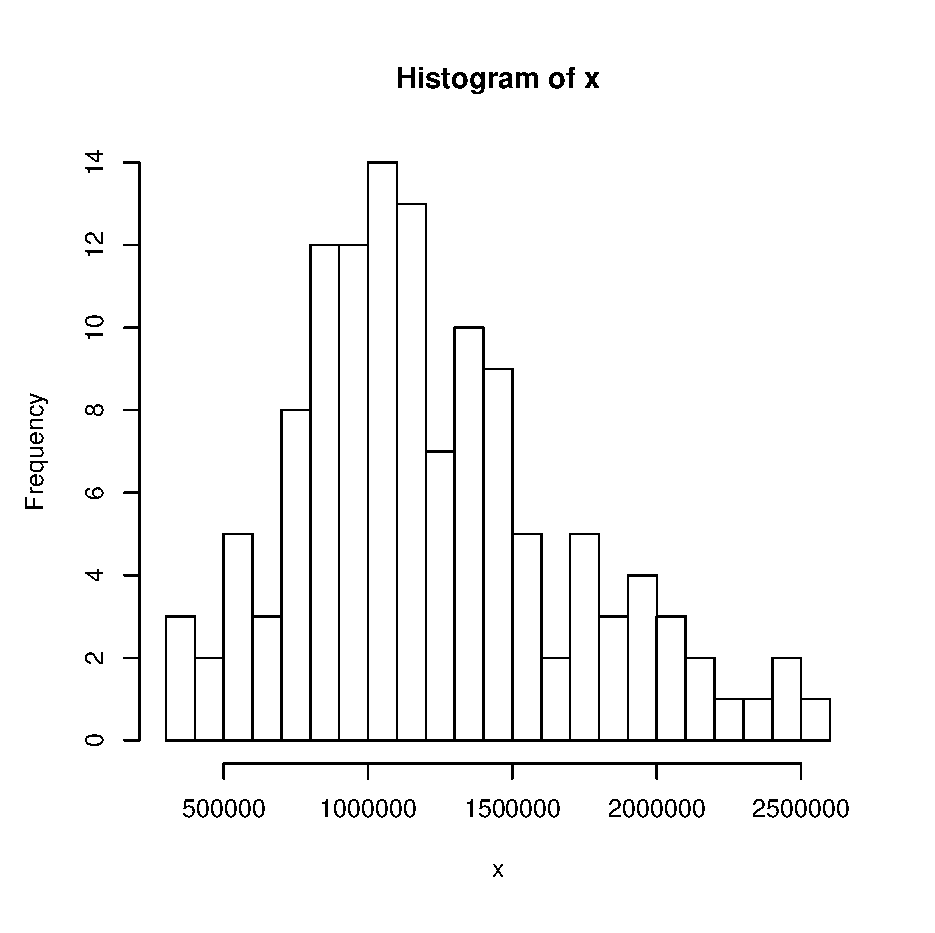
\includegraphics[scale=0.6]{ejemplo_gamma.eps}
\caption{\textsl{Histograma de los datos del Ejemplo 2.3.15.}}
\end{figure}

Para estimar los par�metros de la distribuci�n Gamma, calculamos los valores de las estad�sticas $\bar{X}$ y $S_n$, �stas son \$1.220.195 y \$479.670.8, y usando �stas calculamos los par�metros estimados usando (\ref{k_gamma}) y (\ref{theta_gamma}), y tenemos que $\hat{k}=6.96$ y $\hat{\theta}=175094.6$. Para visualizar el ajuste de la distribuci�n $Gamma(6.96,175094.6)$ a los datos, graficamos la funci�n de densidad de esta distribuci�n usando los siguientes c�digos en R y la gr�fica resultante se muestra en la Figura 2.8 donde podemos ver que la funci�n de densidad se asemeja bastante al histograma de los datos presentado anteriormente.
\begin{verbatim}
> gama.densidad<-function(x){
+ fx<-dgamma(x,shape=k,scale=the)
+ }
>
> hist(x,breaks=20,freq=F)
> curve(gama.densidad(x),add=T)
## donde x contiene los 127 datos muestrales
\end{verbatim}

\begin{figure}[!htb]
\centering
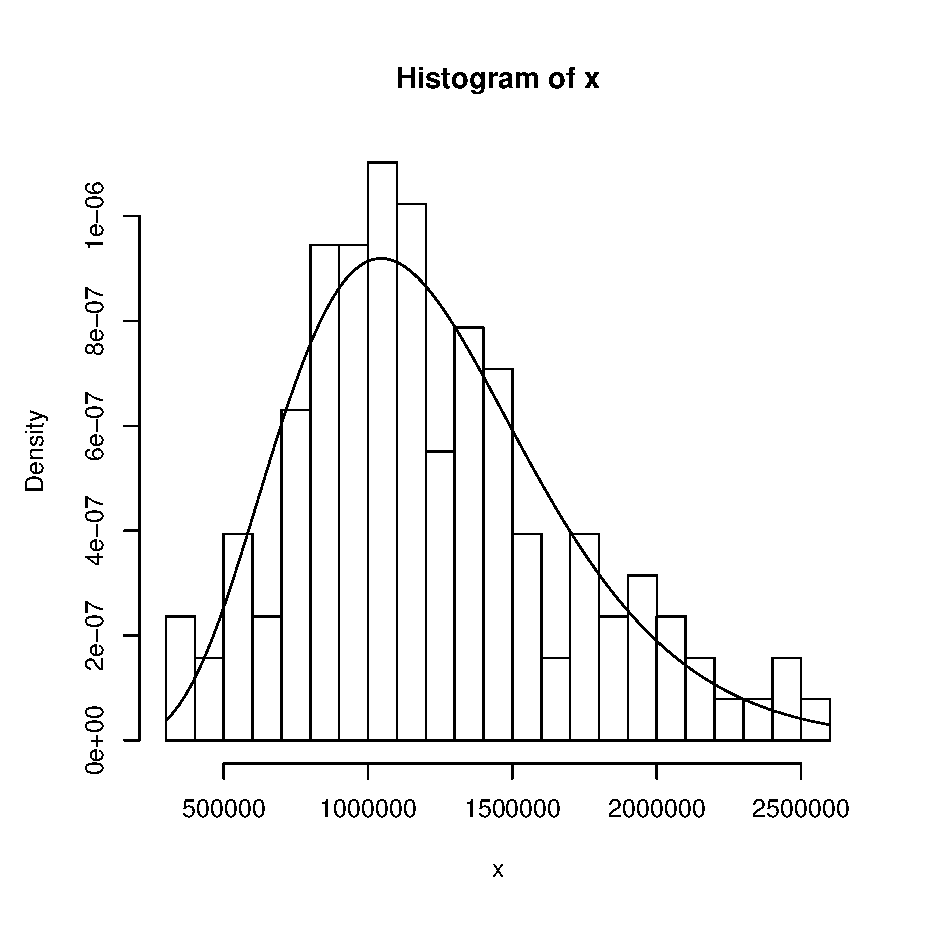
\includegraphics[scale=0.6]{ejemplo_gamma1.eps}
\caption[\textsl{Densidad estimada Gamma de los datos del Ejemplo 2.3.15}]{\textsl{Funci�n de densidad de la distribuci�n Gamma estimada de los datos del Ejemplo 2.3.15.}}
\end{figure}

Ahora, suponga que el instituto conoce que con el aumento los estudiantes con ingreso superior a \$2.000.000 no tendr�n dificultad para pagar el costo de la nueva matr�cula, entonces una estimaci�n del porcentaje de estos estudiantes puede ayudar a los directivos del instituto a prever los efectos del aumento. Como la distribuci�n te�rica identificada es la distribuci�n $Gamma(6.96,175094.6)$, podemos calcular este porcentaje como $Pr(X>1500000)$ donde $X\sim Gamma(6.96,175094.6)$. Esta pro\-ba\-bi\-li\-dad se puede calcular usando el comando
\begin{verbatim}
> pgamma(2000000,shape=6.96, scale=175094.6,lower.tail = F)
[1] 0.06111038
\end{verbatim}
Y tenemos que aproximadamente el 6.1\% de estudiantes de este instituto tiene un ingreso mensual superior a \$2.000.000. Dado que este porcentaje es bastante peque�o, los directivos deber�an plantear un aumento menos dr�stico para evitar el efecto de deserci�n estudiantil.
\end{Eje}

\newpage
\begin{Eje}
Dada una muestra aleatoria $X_1$, $\cdots$, $X_n$ proveniente de una distribuci�n $Beta(a,b)$, entonces la esperanza y la varianza de la distribuci�n te�rica est�n dadas por\index{Estimador!de momentos!Beta}
\begin{equation}\label{mu_beta}
\mu=\frac{a}{a+b}
\end{equation}
y
\begin{equation*}
\sigma^2=\frac{ab}{(a+b+1)(a+b)^2}
\end{equation*}
Para encontrar los estimadores de momentos de $a$ y $b$ se debe escribir a estos en t�rminos de $\mu$ y $\sigma^2$. Para eso tenemos que
\begin{align*}
\sigma^2&=\mu\frac{b}{(a+b-1)(a+b)}\\
&=\mu(1-\mu)\frac{1}{a+b-1}
\end{align*}

De donde
\begin{equation*}
a+b=\frac{\mu(1-\mu)}{\sigma^2}-1
\end{equation*}

Reemplazando lo anterior en (\ref{mu_beta}) tenemos que
\begin{equation*}
a=\mu(a+b)=\frac{\mu^2(1-\mu)}{\sigma^2}-\mu
\end{equation*}
y
\begin{equation*}
b=\frac{\mu(1-\mu)}{\sigma^2}-1-a=(1-\mu)\left(\frac{\mu(1-\mu)}{\sigma^2}-1\right)
\end{equation*}

Y utilizando los principios del m�todo de los momentos de estimar $\mu$ y $\sigma^2$ con $\bar{X}$ y $S^2_n$, tenemos los siguientes estimadores de momentos de $a$ y $b$
\begin{equation*}
\hat{a}_{mom}=\frac{\bar{X}^2(1-\bar{X})}{S^2_n}-\bar{X}
\end{equation*}

y
\begin{equation*}
b=(1-\bar{X})\left(\frac{\bar{X}(1-\bar{X})}{S^2_n}-1\right)
\end{equation*}

Como una aplicaci�n de la distribuci�n Beta, suponga que un almac�n de cadena de ropa femenina investiga acerca de las prendas que son devueltas por los clientes despu�s de la venta. En el caso de que se observe un gran porcentaje de devoluciones, los directivos del almac�n estudiar�n las causas que pueden ser mala calidad de las prendas por parte del proveedor, precios muy altos comparados con productos de la misma categor�a o inclusive vendedores muy h�biles pueden disuadir a los clientes a�n cuando no quieren realizar la compra y �stos pueden arrepentir posteriormente y efectuar la devoluci�n de la compra.

Con el fin de llevar a cabo la investigaci�n, los directivos disponen de porcentaje de prendas devueltas en un mes para diferentes sucursales. Estos datos son:  0.7\%, 0.14\%, 19.7\%, 0.1\%, 12.4\%, 1.1\%, 0.5\%, 18.9\%, 5.0\%, 0.3\%, 0.6\%, 5.4\%, 6.7\% y 0.9\%. Dado que los datos son porcentajes y los porcentajes siempre est�n dentro del intervalo $[0,1]$, podemos pensar que una distribuci�n Beta puede ser apropiada para describir a estos datos. Observemos el histograma en la Figura 2.9 de los datos para verificar si esta distribuci�n es adecuada o no.

\begin{figure}[!htb]
\centering
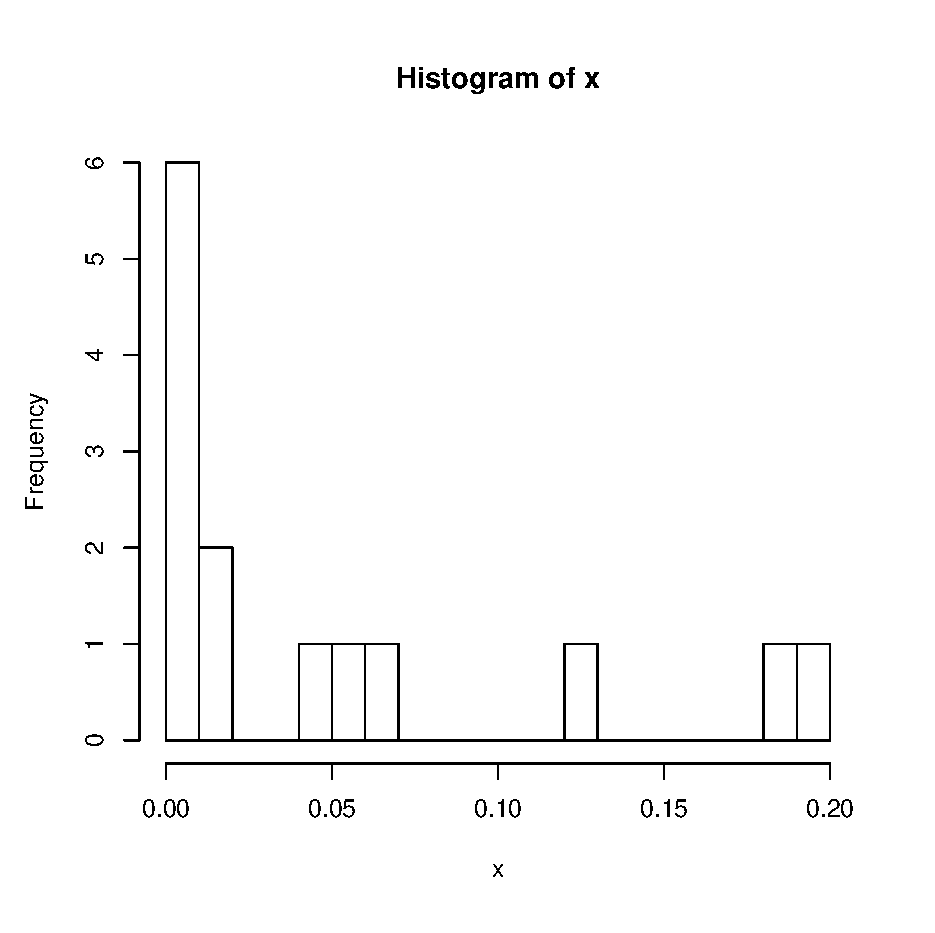
\includegraphics[scale=0.6]{ejemplo_beta1.eps}
\caption{\textsl{Histograma de los datos del Ejemplo 2.3.16.}}
\end{figure}

Podemos ver que la gr�fica es altamente no sim�trica, de donde se descarta la distribuci�n normal para describir a los datos. Sin embargo, podr�amos pensar que una distribuci�n exponencial puede ser apropiada dado que el histograma de los datos se asemeja a la funci�n de densidad de esta distribuci�n. Tenemos una herramienta �til para verificar si una distribuci�n exponencial puede ser apropiada para los datos que es la gr�fica QQ plot. Esta gr�fica para los datos de este ejemplo se muestra en la Figura 2.10 donde se observa que la mayor�a de datos est�n situados por debajo de la recta, lo cual indica que la distribuci�n exponencial no describe bien el comportamiento de los datos, y por consiguiente tambi�n est� descartada.

\begin{figure}[!htb]
\centering
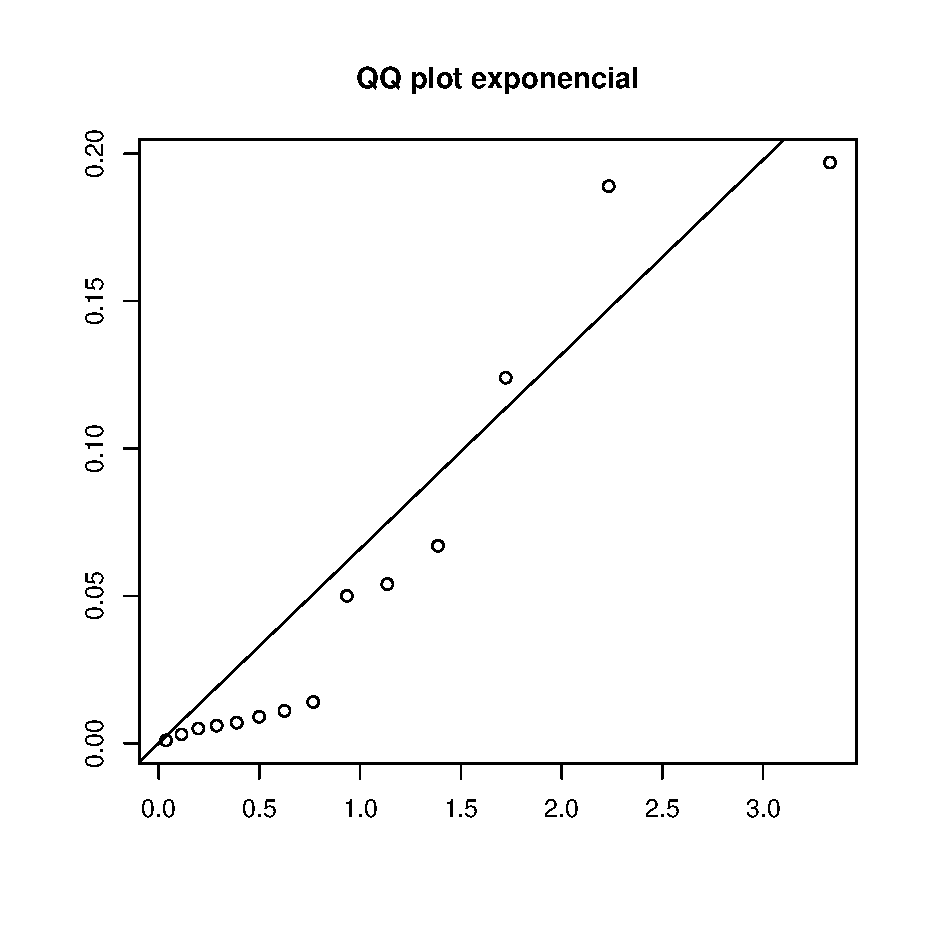
\includegraphics[scale=0.6]{ejemplo_beta2.eps}
\caption[\textsl{QQ plot exponencial para datos del Ejemplo 2.3.16.}]{\textsl{QQ plot para verificar la distribuci�n exponencial para los datos del Ejemplo 2.3.16.}}
\end{figure}

Dado lo anterior, podemos intentar utilizar la distribuci�n Beta para describir este conjunto de datos. Primero calcularemos las estimaciones de los par�metros de la distribuci�n Beta mediante el siguiente c�digo.
\newpage
\begin{verbatim}
> x<-c(0.7, 1.4, 19.7, 0.1, 12.4, 1.1, 0.5, 18.9, 5.0, 0.3,
+   0.6, 5.4, 6.7, 0.9)/100
> n<-length(x)
> va<-var(x)*(n-1)/n
> bar<-mean(x)
> a<-bar^2*(1-bar)/va-bar
> a
[1] 0.5447021
> b<-(1-bar)*(bar*(1-bar)/va-1)
> b
[1] 9.80242
\end{verbatim}

De lo anterior, tenemos las estimaciones de 0.03 y 0.46 para los par�metros de la distribuci�n Beta. Podemos visualizar la forma de la funci�n de densidad Beta con estos par�metros y ver que tenga aspectos similares con el histograma de los datos. Lo anterior se puede llevar a cabo usando los siguientes c�digos.
\begin{verbatim}
> hist(x,breaks=20,freq=F)
> curve(dbeta(x,a,b),add=T)
\end{verbatim}

\begin{figure}[!htb]
\centering
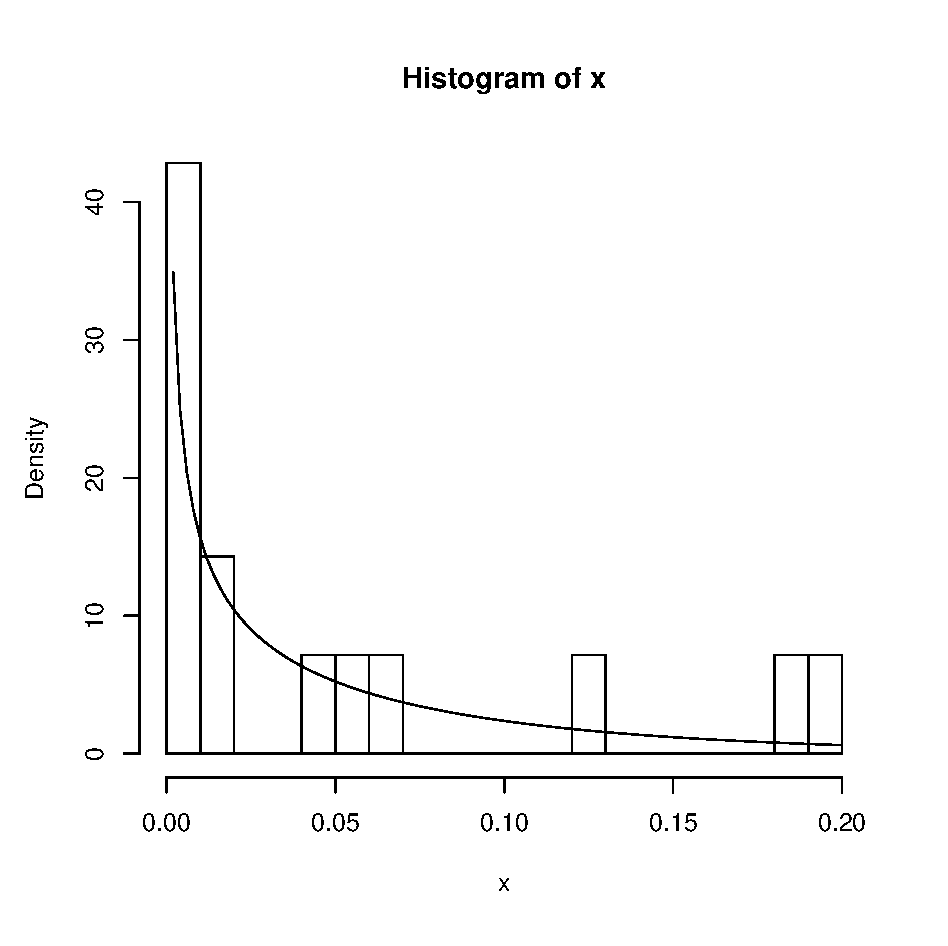
\includegraphics[scale=0.6]{ejemplo_beta.eps}
\caption[\textsl{Datos y densidad estimada del Ejemplo 2.3.16}]{\textsl{Histograma de los datos (a) y la funci�n de densidad estimada (b) de los datos del Ejemplo 2.3.16.}}
\end{figure}

Y como se puede observar en la Figura 2.11, la funci�n de densidad de la distribuci�n $Beta(0.03,0.46)$ parece ser apropiada para los datos observados. Ahora, si se quiere estimar el porcentaje promedio de prendas devueltas, esto es, la esperanza de la distribuci�n te�rica, podemos utilizar simplemente $\bar{x}=0.052=5.2\%$, o equivalentemente la expresi�n (\ref{mu_beta}) dada por $\hat{a}/(\hat{a}+\hat{b})=0.052=5.2\%$.
\end{Eje}

En los ejemplos anteriores, se vio que en la distribuci�n normal, los estimadores de momentos coinciden con los de m�xima verosimilitud, situaci�n que tambi�n ocurre en la distribuci�n Poisson, exponencial y Bernoulli\footnote{En general, el estimador de momentos no es �nico, por ejemplo en la distribuci�n Poisson, el estimador de momentos $\bar{X}$ coincide con el obtenido con el m�todo de m�xima verosimilitud, pero puede haber otros estimadores de momentos diferentes que $\bar{X}$} (Ejercicios 2.3 y 2.6). Sin embargo, en muestras provenientes de algunas distribuciones del tipo uniforme, el estimador de momentos puede no coincidir con el estimador de m�xima verosimilitud, como lo ilustra el siguiente ejemplo.

\begin{Eje}
\index{Estimador!de momentos!uniforme}Dada una muestra aleatoria $X_1$, $\cdots$, $X_n$ proveniente de una distribuci�n uniforme continua sobre $(0,\theta)$. Para encontrar el estimador de momentos de $\theta$, se tiene en cuenta que $\mu=\theta/2$, de donde $\theta=2\mu$, entonces se concluye que $\hat{\theta}_{mom}=2\bar{X}$, el cual es diferente que el estimador de m�xima verosimilitud dada por $\hat{\theta}_{MV}=X_{(n)}$. En la siguiente secci�n, se estudiar� cu�l de estos dos estimadores es mejor. Sin embargo, podemos realizar un peque�o estudio simulaci�n: se simulan muestras de tama�o 5, $\cdots$, 300 de las distribuciones $Unif(0,3)$ y $Unif(0,5)$, en cada muestra simulada se calculan el estimador de momentos y de m�xima verosimilitud. Estas simulaciones se pueden llevar a cabo modificando levemente los c�digos en R presentados en la p�gina 90 . Las estimaciones resultantes se observan en la Figura 2.12, donde la l�nea negra horizontal denota el valor verdadero del par�metro. Podemos ver que con el estimador de m�xima verosimilitud siempre se obtuvieron valores m�s cercanos al par�metro sin importar el tama�o muestral, aunque las estimaciones de m�xima verosimilitud parecen estar por debajo del $\theta$ verdadero, situaci�n que no sucede con las estimaciones de momentos. Este hecho se confirmar� en la siguiente secci�n mediante desarrollos te�ricos.
\begin{figure}[!htb]
\centering
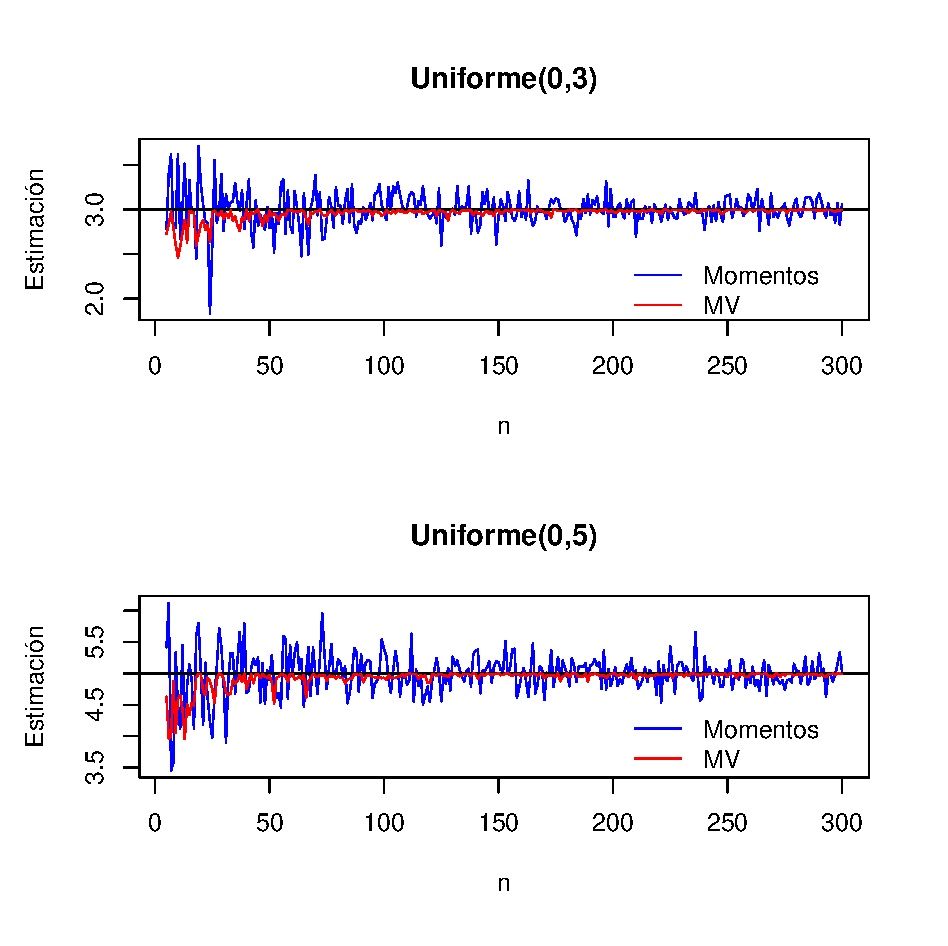
\includegraphics[scale=0.6]{estimadores1_uniforme.eps}
\caption[\textsl{El estimador de MV y el de momentos en muestras uniforme}]{\textsl{Comparaci�n entre el estimador de m�xima verosimilitud y el de momentos en muestras provenientes de distribuciones $Unif(0,3)$ y $Unif(0,5)$.}}
\end{figure}
\end{Eje}

An�logo al m�todo de m�xima verosimilitud, en el m�todo de los momentos tambi�n podemos garantizar la invarianza del\index{Estimador!de momentos!invarianza} estimador obtenido para cualquier funci�n del par�metro $g(\theta)$. Suponga que el tiempo de llegada de un bus a cierta estaci�n contada desde las ocho de la ma�ana sigue una distribuci�n $Unif(0,\theta)$. Con esta distribuci�n, estamos suponiendo que el tiempo de llegada toma valor en cualquier intervalo de longitud fijo de $(0,\theta)$ con la misma probabilidad. Se ha visto en el ejemplo anterior que $\hat{\theta}_{mom}=2\bar{X}$, y si la cantidad que se desea estimar es la probabilidad de que el bus llegue en menos de un minuto, entonces estamos interesados en estimar $p=1/\theta$, y $p$ puede ser escrito en funci�n del primer momento, puesto que $p=1/(2\mu)$. De esta forma, aplicando los principios del m�todo de los momentos, se tiene que $\hat{p}_{mom}=1/(2\bar{X})$.

Para concluir el m�todo de los momentos, damos dos ejemplos interesantes acerca de la distribuci�n uniforme.

\begin{Eje}
\index{Estimador!de momentos!uniforme}Suponga que una muestra aleatoria $X_1$, $\cdots$, $X_n$ proviene de la distribuci�n $U[-\theta,\theta]$, en este caso la esperanza es 0, y no depende del par�metro $\theta$, por lo tanto, no hay forma de escribir a $\theta$ en funci�n de la esperanza. Pero podemos recurrir a la varianza de la distribuci�n uniforme, notando que la varianza es $\theta^2/3$, de donde se tiene que $\theta=\sqrt{3\sigma^2}$ (la soluci�n $\theta=-\sqrt{3\sigma^2}$ claramente no puede ser el par�metro de la distribuci�n, puesto que $\theta$ debe ser positivo), en conclusi�n un estimador de momentos de $\theta$ es $\sqrt{3S^2_n}$. Por otro lado, se puede ver que el estimador de m�xima verosimilitud de $\theta$ est� dado por $\max\{-X_{(1)},X_{(n)}\}$ (Ejercicio 2.11).

En la Figura 2.13, se observan resultados de muestras de tama�o 5, $\cdots$, 300 simulados de una distribuci�n $Unif[-3,3]$ y en cada muestra simulada se calcula el estimador de momentos y de m�xima verosimilitud. Podemos observar que en muestras peque�as los resultados obtenidos con el estimador de m�xima verosimilitud casi siempre est�n por debajo del par�metro causando el problema de subestimaci�n. A medida que las muestras se hacen grandes el m�todo de m�xima verosimilitud parece funcionar mejor; por otro lado, aunque los valores obtenidos con el m�todo de los momentos no parecen tener el problema de subestimaci�n que s� tiene el de m�xima verosimilitud, los valores obtenidos con el m�todo de los momentos son muy dispersos, y hay muestras donde la estimaci�n puede estar realmente lejos del par�metro.

\begin{figure}[!htb]
\centering
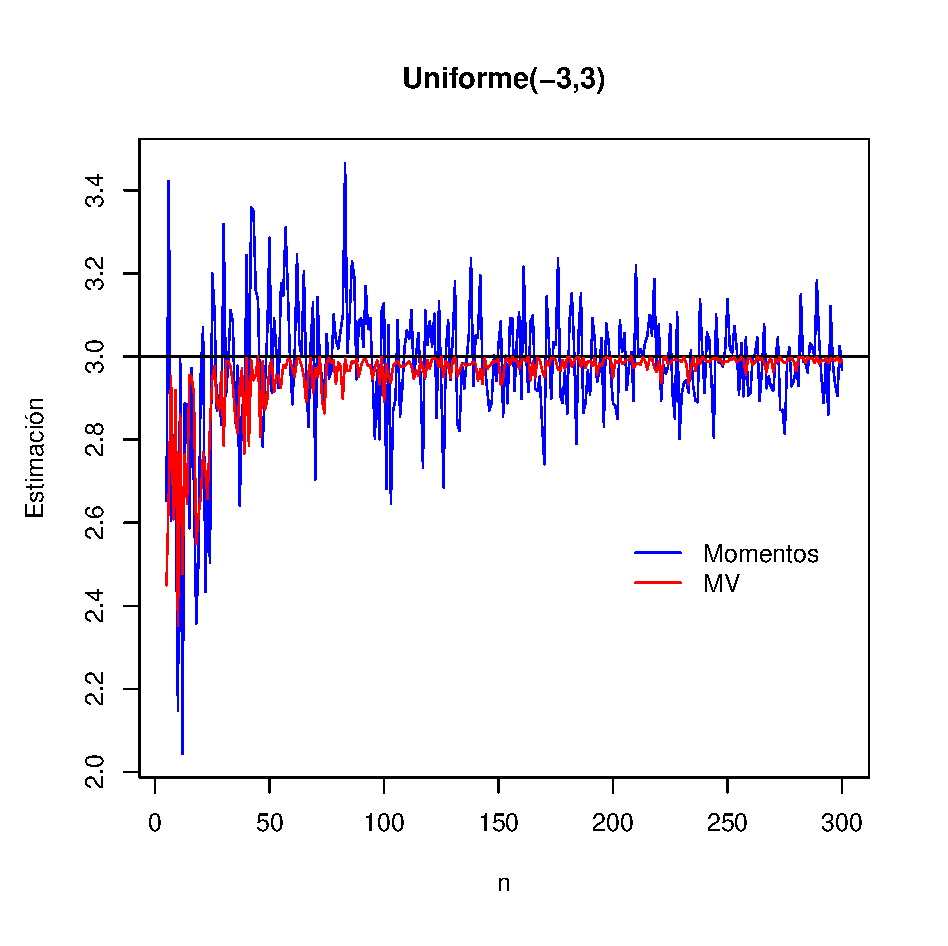
\includegraphics[scale=0.5]{estimadores_uniforme.eps}
\caption[\textsl{El estimador de MV y el de momentos en muestras uniforme}]{\textsl{Comparaci�n entre el estimador de m�xima verosimilitud y el de momentos en muestras provenientes de la distribuci�n $Unif(-3,3)$.}}
\end{figure}
\end{Eje}

En el anterior ejemplo se vio que en algunas ocasiones en el m�todo de los momentos puede no ser �til evaluar el primer momento sino usando el segundo momento (o equivalentemente la varianza de la distribuci�n te�rica). En el siguiente ejemplo, ilustramos un caso donde el procedimiento est�ndar del m�todo de los momentos arroja dos soluciones y se debe tener en cuenta el espacio param�trico de los par�metros de inter�s para escoger la soluci�n apropiada.

\begin{Eje}
\index{Estimador!de momentos!uniforme}Suponga que una muestra aleatoria $X_1$, $\cdots$, $X_n$ proviene de la distribuci�n $U[\theta_1,\theta_2]$, donde $\theta_1$ y $\theta_2$ son desconocidos. Para estimar estos par�metros v�a el m�todo de los momentos, necesitamos escribirlos en t�rmino de la media $\mu$ y la varianza $\sigma^2$. Usando el Resultado 1.1.11, tenemos que
\begin{equation*}
\begin{cases}
\mu=\dfrac{\theta_1+\theta_2}{2}\\
\sigma^2=\dfrac{(\theta_2-\theta_1)^2}{12},
\end{cases}
\end{equation*}
y tenemos dos soluciones para $\theta_1$ y $\theta_2$, estas son $\begin{cases}
\theta_1=\mu-\sqrt{3}\sigma\\
\theta_2=\mu+\sqrt{3}\sigma
\end{cases}$
o $\begin{cases}
\theta_1=\mu+\sqrt{3}\sigma\\
\theta_2=\mu-\sqrt{3}\sigma
\end{cases}.$
N�tese que en la segunda soluci�n $\theta_1>\theta_2$, no cumple con el supuesto de una distribuci�n $U[\theta_1,\theta_2]$, y por consiguiente, usaremos la primera soluci�n, y los estimadores de momentos de $\theta_1$ y $\theta_2$ ser�n $\bar{X}-\sqrt{3}S_n$ y $\bar{X}+\sqrt{3}S_n$, respectivamente. Se puede ver f�cilmente que los estimadores de m�xima verosimilitud de $\theta_1$ y $\theta_2$ son $X_{(1)}$ y $X_{(n)}$ (Ejercicio 2.13).
\end{Eje}

\subsection{M�todo de m�nimos cuadrados\index{M�todo de m�nimos cuadrados}}
El m�todo de m�nimos cuadrados es un m�todo muy com�n en la teor�a del modelamiento estad�stico, aqu� se hace una breve introducci�n utilizando este m�todo para estimar la esperanza de una distribuci�n te�rica.

\begin{Defi}
Dado un conjunto de datos $x_1$, $\cdots$, $x_n$, una medida de dispersi�n es una funci�n que satisface las siguientes propiedades
\begin{enumerate}
\item $D(\mathbf{x}+\mathbf{1}_nc)=D(\mathbf{x})$
\item $D(-\mathbf{x})=D(\mathbf{x})$
\end{enumerate}

donde $\mathbf{x}$ es el vector conformado por los $n$ datos, $\mathbf{1}_n$  es el vector de unos de tama�o $n$ y $c$ es cualquier n�mero real.
\end{Defi}

\begin{Eje}
Las varianzas $S^2_n$, $S^2_{n-1}$ y las respectivas desviaciones est�ndares son medidas de dispersi�n. Puesto que en primer lugar, si se traslada a un conjunto de datos agregando una constante $c$ $S^2_n$ y $S^2_{n-1}$ no cambian de valor; en segundo lugar, estas varianzas tampoco cambian de valor si se multiplica por $-1$ a todos los datos.
\end{Eje}

Ahora introducimos el m�todo de m�nimos cuadrados para estimar la esperanza de una distribuci�n te�rica $\mu$ bas�ndonos en una muestra $X_1$, $\cdots$, $X_n$. Dado que $\mu$ es la media te�rica, se espera que los valores de la muestra observada est�n cercanos a $\mu$, por lo tanto, podemos proponer estimar $\mu$ como el valor que m�s se acerque a los datos. Una forma de medir la distancia entre dos puntos es la distancia euclidiana, as� podemos estimar $\mu$ como aquel que minimiza la cantidad
\begin{equation*}
Q=\sum_{i=1}^n(x_i-\mu)^2.
\end{equation*}

De lo anterior, es claro el origen del nombre de estimador de m�nimos cuadrados\index{Estimador!de m�nimos cuadrados}.

\begin{Res}
Sea $X_1$, $\cdots$, $X_n$ una muestra aleatoria proveniente de una distribuci�n con media te�rica $\mu$, entonces el estimador de m�nimos cuadrados de $\mu$ es $\bar{X}$.\index{Estimador!de m�nimos cuadrados!media te�rica}
\end{Res}

\begin{proof}
Derivando $Q$ con respecto a $\mu$ e igualando a cero, tenemos que
\begin{equation}
\frac{\partial Q}{\partial\mu}=-2\sum_{i=1}^n(x_i-\mu)=0
\end{equation}

el cual conduce a la soluci�n de $\mu=\bar{X}$, de donde tenemos que el estimador de la media te�rico bajo cualquier distribuci�n est� dado por
\begin{equation*}
\hat{\mu}_{MC}=\bar{X}.
\end{equation*}
\end{proof}

\section{Propiedades de estimadores puntuales}

En la anterior secci�n, se observ� que para estimar un par�metro $\theta$, el m�todo de m�xima verosimilitud y el de momentos pueden conducir a estimadores diferentes; m�s a�n, se pueden crear muchos otros tipos de estimadores para $\theta$, pues un estimador es simplemente una estad�stica que es usada para estimar. Por ejemplo, dada una muestra aleatoria $X_1$, $\cdots$, $X_{20}$ con media te�rica $\mu$ desconocido, un estimador razonable para $\mu$ es la media muestral $\bar{X}$; sin embargo, alguien puede querer usar la estad�stica $\sum X_i$ para estimar $\mu$, otro puede preferir algo como $\exp\{\sum X_i\}$, otra persona puede inventar su propio estimador, entonces �c�mo se puede escoger el mejor estimador entre un conjunto de estimadores?, �qu� aspectos y propiedades se deben tener en cuenta para esa escogencia? El objetivo de este cap�tulo es introducir conceptos que contestan estas preguntas.

\subsection{Error cuadr�tico medio}

Consideramos la siguiente situaci�n hipot�tica. Suponga que para estimar un par�metro $\theta$, se disponen de tres estimadores $T_1$, $T_2$ y $T_3$, y adem�s suponga que las respectivas estimaciones en 7 muestras observadas de la poblaci�n son los valores dados en la Tabla 2.2.
\begin{table}
\centering
\begin{tabular}{cccc}\hline
Muestra&$T_1$&$T_2$&$T_3$\\\hline
1&4.1&5.5&5.1\\
2&4.3&5.6&5.0\\
3&5.6&5.4&4.8\\
4&5.3&5.5&4.9\\
5&4.5&5.4&5.2\\
6&4.7&5.6&5.0\\
7&5.7&5.5&4.9\\\hline
promedio&4.88&5.5&4.99\\
desviaci�n&0.64&0.08&0.13\\\hline
\end{tabular}\caption{\textsl{Valores de tres estimadores en 7 muestras diferentes.}}
\end{table}

Y adem�s suponga que el valor verdadero de $\theta$ es 5, �cu�l estimador es mejor dadas las anteriores estimaciones? Para responder esta pregunta, observamos lo siguiente con respecto a los tres estimadores:
\begin{itemize}
      \item Los valores que toma $T_1$ en promedio est�n cerca del 5, pero estos est�n muy alejados entre s�, es decir, tienen una dispersi�n grande. Esta dispersi�n grande es una propiedad indeseada del estimador, pues generalmente en la pr�ctica, tenemos solo una muestra, una dispersi�n grande entre los valores de $T_1$ implica que hay mayor probabilidad de que $T_1$ tome un valor alejado del par�metro en una muestra.
      \item Los valores que toma $T_2$ est�n alrededor del 5.5, muy por encima del valor verdadero de $\theta$, 5, esta situaci�n se llama la sobreestimaci�n. Por otro lado, en t�rminos de la dispersi�n, se observa que los valores est�n altamente concentrados.
      \item Los valores que toma $T_3$, en primer lugar, est�n alrededor del 5, adem�s de tener una dispersi�n peque�a. Lo anterior indica que en todas las muestras, el valor de $T_3$ est� cercano del valor de $\theta$. Y podemos concluir que el mejor estimador de los tres es el $T_3$.
\end{itemize}

La anterior situaci�n nos ilustra que un buen estimador $T$ debe tener dos propiedades
\begin{enumerate}
    \item Los valores que toma $T$ en promedio deben ser cercanos al par�metro $\theta$. Teniendo en cuenta que la esperanza de una variable puede ser interpretada como un promedio ponderado de todos los valores que toma la variable, podemos concluir que $T$ debe cumplir con $E(T)=\theta$,
    \item La varianza de $T$ debe ser peque�a.
\end{enumerate}

Ahora damos la siguiente definici�n que describe la propiedad 1.
\begin{Defi}
Dada una muestra aleatoria $X_1$, $\cdots$, $X_n$ proveniente de una distribuci�n con par�metro desconocido $\theta$, y sea $T$ un estimador de $\theta$, se define el sesgo\index{Sesgo} de $T$ como $B_T=E(T)-\theta$.

Cuando $B_T=0$ o equivalentemente $E(T)=\theta$, se dice que el estimador $T$ es insesgado\index{Estimador!insesgado} para $\theta$. Cuando $B_T>0$ o equivalentemente $E(T)>\theta$, se dice que $T$ sobreestima\index{Estimador!sobreestimaci�n} a $\theta$, es decir, en promedio la estimaci�n obtenida usando $T$ es mayor que $\theta$. An�logamente se dice que $T$ subestima\index{Estimador!subestimaci�n} a $\theta$ cuando $B_T<0$.
\end{Defi}

Dada la anterior definici�n, en primera instancia, se necesitan estimadores con sesgo peque�o, y si es posible, insesgados. Adicionalmente, se espera que un buen estimador tenga varianza peque�a. De esta forma, si entre dos estimadores $T_1$ y $T_2$, $T_1$ tiene sesgo y varianza ambos menores que $T_2$, podemos concluir f�cilmente que $T_1$ es mejor que $T_2$. Pero cuando $T_1$ tiene sesgo menor, pero varianza mayor que $T_2$, no es f�cil determinar cu�l es mejor. En este caso, podemos usar el siguiente criterio que combina tanto al sesgo como a la varianza de un estimador.

\begin{Defi}
Dada una muestra aleatoria $X_1$, $\cdots$, $X_n$ proveniente de una distribuci�n con par�metro desconocido $\theta$, y sea $T$ un estimador de $\theta$, se define el error cuadr�tico medio de $T$ como $ECM_T=E(T-\theta)^2$\index{Error cuadr�tico medio}.
\end{Defi}

N�tese que en la anterior definici�n, cuando un estimador $T$ es insesgado para $\theta$, se tiene que $ECM_T=E(T-E(T))^2$, esto es, el error cuadr�tico medio es la varianza del estimador $T$.

M�s aun, el criterio del error cuadr�tico medio combina al sesgo y la varianza, tenemos que
\begin{align*}
ECM_T&=E[T-E(T)+E(T)-\theta]^2\\
     &=E[(T-E(T))^2+2(T-E(T))(E(T)-\theta)+(E(T)-\theta)^2]\\
     &=E[(T-E(T))^2]+2(E(T)-\theta)\underbrace{E[T-E(T)]}_{\text{igual a 0}}+(E(T)-\theta)^2\\
     &=Var(T)+B_T^2
\end{align*}
Entonces un buen estimador debe tener el error cuadr�tico medio peque�o, y para los estimadores insesgados, se necesita que la varianza sea peque�a.

Ahora, al principio del cap�tulo, afirmaba que es natural estimar la media te�rica $\mu$ con la media muestral $\bar{X}$, �qu� tan buena es esta idea? El siguiente resultado nos permite examinar el comportamiento de $\bar{X}$ como estimador de $\mu$.

\begin{Res}
Sea una muestra aleatoria $X_1$, $\cdots$, $X_n$ proveniente de una distribuci�n con media $\mu$ y varianza $\sigma^2$, entonces
\begin{enumerate}
    \item si se considera a $\bar{X}$ como el estimador de $\mu$, se tiene que $\bar{X}$ es insesgado para $\mu$, es decir, $E(\bar{X})=\mu$ y adem�s $Var(\bar{X})=\sigma^2/n$.\index{Estimador!insesgado!media muestral}
    \item si se considera a $S^2_n$ y $S^2_{n-1}$ como estimadores de $\sigma^2$, se tiene que $S^2_n$ es sesgado para $\sigma^2$ donde el sesgo es $-\dfrac{\sigma^2}{n}$; y $S^2_{n-1}$ es insesgado para $\sigma^2$.
\end{enumerate}

\end{Res}
\begin{proof}
La demostraci�n de la parte 1 es trivial, y se deja como ejercicio. Para ver la parte 2, tenemos que
\begin{align*}
E(S^2_n)&=\dfrac{1}{n}E\left(\sum_{i=1}^n(X_i-\bar{X})^2\right)\\
&=\dfrac{1}{n}E\left(\sum_{i=1}^nX_i^2-n\bar{X}^2\right)\\
&=\dfrac{1}{n}\left\{\sum_{i=1}^n\left[Var(X_i)+(E(X_i))^2\right]-nE(\bar{X})^2\right\}\\
&=\dfrac{1}{n}\left\{n\sigma^2+n\mu^2-n\left[\dfrac{\sigma^2}{n}+\mu^2\right]\right\}\\
&=\dfrac{n-1}{n}\sigma^2,
\end{align*}
de donde se concluye que $S^2_n$ es sesgado para $\sigma^2$ con sesgo $-\dfrac{\sigma^2}{n}$. Con respecto a $S^2_{n-1}$, al observar que \begin{equation*}
S^2_{n-1}=\dfrac{n}{n-1}S^2_n,
\end{equation*}
se tiene que $E(S^2_{n-1})=\sigma^2$ y por consiguiente es insesgado para $\sigma^2$.
\end{proof}

N�tese en primer lugar que en el anterior resultado, no se ha especificado la distribuci�n de probabilidad en la poblaci�n, entonces podemos aplicarlo para muestras que provienen de cualquier distribuci�n de probabilidad. En particular, en muestras provenientes de la distribuci�n $Exp(\theta)$, $Pois(\theta)$, $Bernoulli(\theta)$, $N(\theta,\sigma^2)$, el estimador de m�xima verosimilitud coincide con el de momentos $\bar{X}$. Usando el anterior resultado, podemos concluir que $\bar{X}$ es insesgado para el par�metro $\theta$ en cualquiera de estas cuatro distribuciones.

Por otro lado, observe que $Var(\bar{X})$ es inversamente proporcional al tama�o muestral $n$, es decir, a medida que la muestra crece, las estimaciones son m�s concentradas alrededor de $\mu$. En la Figura 2.14, se muestra un estudio de simulaci�n donde se simularon muestras de tama�os 1, $\cdots$, 300, provenientes de distribuci�n normal y exponencial, y en cada muestra se calcula el promedio muestral. Se observa que entre m�s grande sea el valor de $n$, m�s concentradas est�n las estimaciones alrededor de la media te�rica $\mu=5$.

\begin{figure}[!htb]
\centering
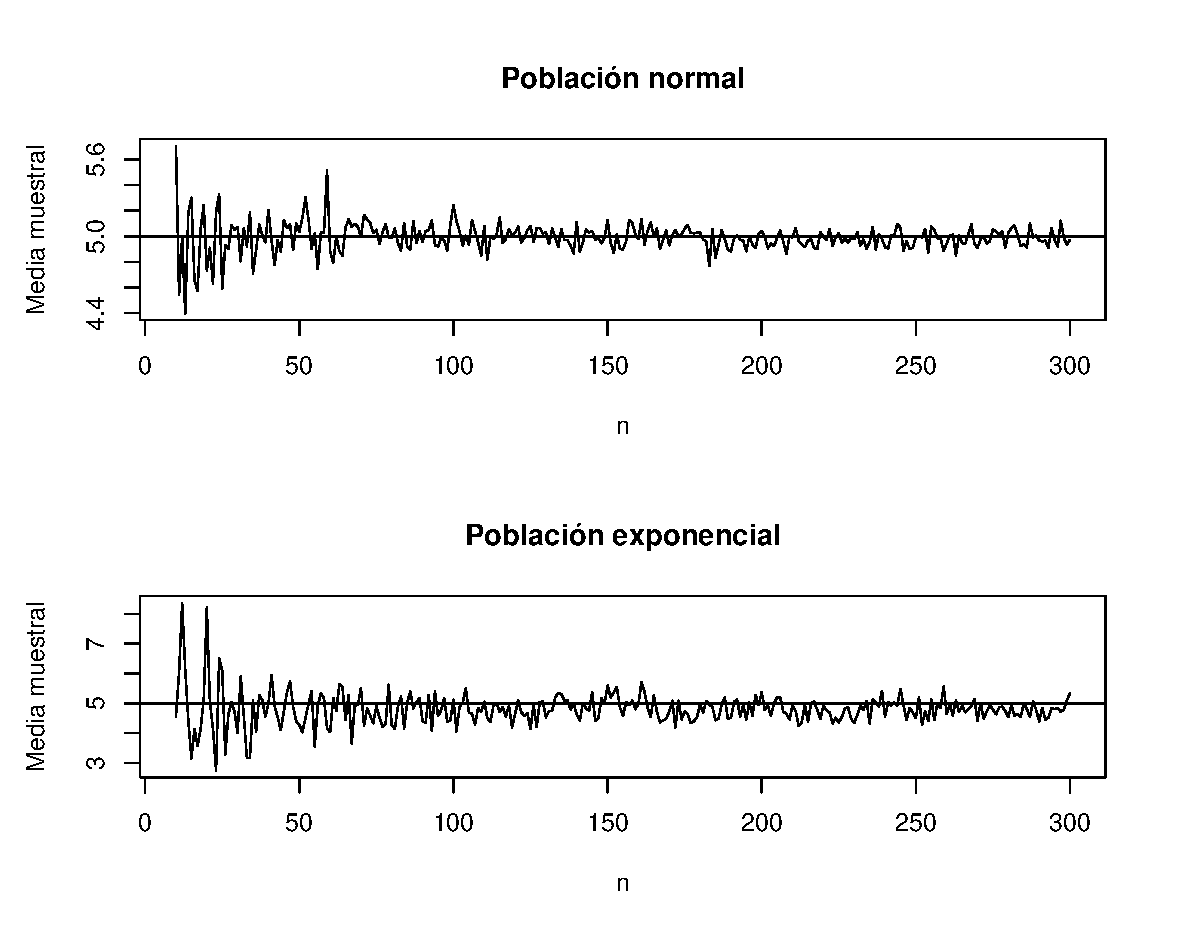
\includegraphics[scale=0.6]{graf1.eps}
\caption{\textsl{Relaci�n entre la estimaci�n de $\mu$ y el tama�o muestral $n$.}}
\end{figure}

Otra observaci�n interesante es que en el contexto del resultado anterior, la variable $X_1$, vista como un estimador de $\mu$ tambi�n es insesgada, puesto que por definici�n de $\mu$, se tiene que $E(X_1)=\mu$; la misma conclusi�n se tiene para $X_i$ para $i=2,\cdots,n$. Es decir, el estimador insesgado para un par�metro puede no ser �nico \footnote{De hecho, si tomamos cualquier subconjunto de la muestra aleatoria, el promedio muestral de este subconjunto ser� un estimador insesgados para $\mu$}. Pero la varianza de $X_i$ con $i=1,\cdots,n$ es $\sigma^2$, que es mayor que $Var(\bar{X})$, de donde se concluye que estos no son tan buenos estimadores como $\bar{X}$.

Ahora, revisamos los estimadores $S^2_n$ y $S^2_{n-1}$ como estimadores de $\sigma^2$. Aunque $S^2_n$ resulta ser sesgado para $\sigma^2$ , el sesgo se hace peque�o cuando el tama�o muestral crece; m�s aun,
\begin{equation*}
\lim_{n\rightarrow\infty}B_{S^2_n}=\lim_{n\rightarrow\infty}-\dfrac{\sigma^2}{n}=0.
\end{equation*}

Estimadores sesgados que cumplen la propiedad $\lim_{n\rightarrow\infty}B_{S^2_n}=0$ son llamados \textsl{asint�ticamente insesgados}\index{Estimador!asint�ticamente insesgado}. Para ilustrar los estimadores $S^2_n$ y $S^2_{n-1}$ en t�rmino de estimaci�n, podemos simular muestras provenientes de una distribuci�n normal de media 5 y desviaci�n est�ndar 9 con tama�os de muestral $n=2,20,30,50,300,$ y en cada muestra calculamos los dos estimadores. El comando utilizado en R es

\begin{verbatim}
>  set.seed(1)
>  n<-c(2,10,30, 50,100, 300, 1000,5000)
>  var1<-rePr(NA,length(n))
>  var2<-rePr(NA,length(n))
>  for(k in 1:length(n))
+   {
+   data<-rnorm(n[k],5,9)
+   var1[k]<-var(data)
+   var2[k]<-(n[k]-1)*var(data)/n[k] }
>   plot(var1,type="b", col=4,ylim=c(min(var2),130),xlab="Tama�o de
+   muestra", ylab="Estimaci�n de la varianza", xaxt="n")
>   lines(var2,type="b", col=2, pch=2)
>   abline(h=81)
>   axis(1, 1:length(n), n)
>   legend(3,120,c("Insesgado","Sesgado"), col=c(4,2), lty=c(1,1),
+   pch=c(1,2))
\end{verbatim}

Y como resultado, obtenemos la Figura 2.15, donde podemos observar que las estimaciones del estimador sesgado $S^2_n$ siempre son inferiores que los del estimador insesgado $S^2_{n-1}$; en segundo lugar, la diferencia entre los dos estimadores se hace cada vez m�s peque�a y los valores de ambos estimadores se acercan al par�metro te�rico a medida que el tama�o muestral crece. Por otro lado, aunque $S^2_n$ subestima la varianza te�rica, en la gr�fica podemos observar que en la muestra simulada del tama�o 300, 1000 y 5000, las estimaciones de $S^2_n$ estuvieron por encima de la varianza te�rica, esto no es ninguna contradicci�n con el hecho de que $S^2_n$ subestima a $\sigma^2$, ya que el concepto de subestimaci�n de un estimador indica que promediando todos los valores del estimador, da un valor inferior al par�metro, mas no indica que todas las estimaciones obtenidas son inferiores al par�metro.

\begin{figure}[!htb]
\centering
\includegraphics[scale=0.5]{est1.eps}
\caption[\textsl{Estimaciones de $S^2_n$ y $S^2_{n-1}$ en muestras de $N(5,9^2)$}]{\textsl{Ilustraci�n de las estimaciones de $S^2_n$ y $S^2_{n-1}$ como estimadores de $\sigma^2$ en muestras provenientes de $N(5,9^2)$.}}
\end{figure}

Finalmente, de la parte dos del Resultado 2.4.1, tambi�n se puede concluir que los estimadores obtenidos mediante el m�todo de m�xima verosimilitud o el de momentos pueden ser sesgados, puesto que una muestra proveniente de la distribuci�n normal, se ha visto que cuando $\mu$ es desconocido, $\hat{\sigma^2}_{MV}=\hat{\sigma^2}_{mom}=S^2_n$, y �sta es sesgada para $\sigma^2$. Sin embargo, en la demostraci�n del Resultado 2.4.1, se vio que en algunos casos, una peque�a modificaci�n al estimador de m�xima verosimilitud o el de momentos puede corregir el sesgo y obtener un estimador insesgado.

El Resultado 2.4.1 es v�lido para muestras provenientes de cualquier distribuci�n; sin embargo, cuando la muestra proviene de una distribuci�n normal, existe el siguiente resultado que nos permite ver que $S^2_n$ es sesgado para $\sigma^2$. Lo presentamos, pues es de gran utilidad para la teor�a desarrollada en los cap�tulos siguientes.

\begin{Res}
Sea $X_1$, $\cdots$, $X_n$ una muestra aleatoria proveniente de $N(\mu,\sigma^2)$, y sea $Y=\dfrac{\sum_{i=1}^n(X_i-\bar{X})^2}{\sigma^2}$, entonces se tiene que $Y\sim\chi^2_{n-1}$.
\end{Res}
\begin{proof}
En primer lugar, consideramos la variable $\sum_{i=1}^n(X_i-\mu)^2$, tenemos
\begin{align*}
\sum_{i=1}^n(X_i-\mu)^2&=\sum_{i=1}^n(X_i-\bar{X}+\bar{X}-\mu)^2\\
                       &=\sum_{i=1}^n(X_i-\bar{X})^2+2(\bar{X}-\mu)\underbrace{\sum_{i=1}^n(X_i-\bar{X})}_{=0}+n(\bar{X}-\mu)^2\\
                       &=\sum_{i=1}^n(X_i-\bar{X})^2+n(\bar{X}-\mu)^2
\end{align*}

Dividiendo $\sigma^2$ en ambos lados, se tiene que \begin{equation*}
\underbrace{\sum_{i=1}^n\dfrac{(X_i-\mu)^2}{\sigma^2}}_{A}=\underbrace{\sum_{i=1}^n\dfrac{(X_i-\bar{X})^2}{\sigma^2}}_{Y}+\underbrace{\dfrac{n(\bar{X}-\mu)^2}{\sigma^2}}_{B}.
\end{equation*}

Si podemos suponer que las variables $S^2_n$ y $\bar{X}$ son independientes, podemos concluir que $\sum_{i=1}^n\dfrac{(X_i-\bar{X})^2}{\sigma^2}$ y $\dfrac{n(\bar{X}-\mu)^2}{\sigma^2}$ tambi�n son independientes. Entonces existe la siguiente relaci�n entre las funciones generadora de momentos de las variables $A$, $Y$ y $B$: $m_A(t)=m_Y(t)m_B(t)$, de donde se obtiene que
\begin{equation}\label{Gene}
m_Y(t)=m_A(t)/m_B(t).
\end{equation}

Ahora, $\dfrac{X_i-\mu}{\sigma}$ son variables con distribuci�n normal est�ndar para $i=1,\cdots,n$, entonces $\sum_{i=1}^n\dfrac{(X_i-\mu)^2}{\sigma^2}$ tiene distribuci�n $\chi^2_{n}$ con funci�n generadora de momentos $(1-2t)^{-n/2}$. Por el otro lado $\bar{X}\sim N(\mu,\sigma^2/n)$, entonces $\dfrac{\sqrt{n}(\bar{X}-\mu)}{\sigma}\sim N(0,1)$, de donde se tiene que $\dfrac{n(\bar{X}-\mu)^2}{\sigma^2}\sim\chi^2_1$ cuya funci�n generadora de momentos es $(1-2t)^{-1/2}$. Reemplazando lo anterior en (\ref{Gene}), se tiene que $m_Y(t)=(1-2t)^{-(n-1)/2}$, lo cual indica que $Y\sim\chi^2_{n-1}$.
\end{proof}

Para completar la demostraci�n del anterior resultado, es necesitario probar la independencia entre $\bar{X}$ y $S^2_n$. Tenemos el siguiente resultado.
\begin{Res}
Dada $X_1$, $\cdots$, $X_n$ una muestra aleatoria proveniente de $N(\mu,\sigma^2)$, se tiene que $\bar{X}$ y $S^2_n$ son independientes.
\end{Res}
\begin{proof}
La demostraci�n de este resultado es tomada de \citeasnoun{Casella}. Se probar� que $\bar{X}$ y $\sum_{i=1}^n(X_i-\bar{X})^2$ son independientes. Tenemos
\begin{align*}
\sum_{i=1}^n(X_i-\bar{X})^2&=(X_1-\bar{X})^2+\sum_{i=2}^n(X_i-\bar{X})^2\\
&=\left[\sum_{i=1}^n(X_i-\bar{X})-\sum_{i=2}^n(X_i-\bar{X})\right]^2+\sum_{i=2}^n(X_i-\bar{X})^2\\
&=\left[\sum_{i=2}^n(X_i-\bar{X})\right]^2+\sum_{i=2}^n(X_i-\bar{X})^2.
\end{align*}
De lo anterior, se observa que $\sum_{i=1}^n(X_i-\bar{X})^2$ puede verse como una funci�n de las variables $X_2-\bar{X}$, $\cdots$, $X_n-\bar{X}$, por lo tanto, basta ver que estas variables son independientes de $\bar{X}$. Sin embargo, las variables $X_1$, $\cdots$, $X_n$ tienen distribuci�n $N(\mu,\sigma^2)$, y la presencia de estos dos par�metros complica un poco los c�lculos, por lo que se trabajar� con las variables estandarizadas, $Z_1$, $\cdots$, $Z_n$, donde el promedio est� dado por
\begin{align*}
\bar{Z}&=\dfrac{1}{n}\sum_{i=1}^nZ_i\\
&=\dfrac{1}{n}\sum_{i=1}^n\dfrac{X_i-\mu}{\sigma}\\
&=\dfrac{1}{n\sigma}\sum_{i=1}^nX_i-\dfrac{\mu}{\sigma}\\
&=\dfrac{\bar{X}}{\sigma}-\dfrac{\mu}{\sigma},
\end{align*}
adem�s $Z_i-\bar{Z}=\dfrac{X_i-\bar{X}}{\sigma}$ para todo $i=2,\cdots,n$. Por lo tanto, para ver que las variables $X_2-\bar{X}$, $\cdots$, $X_n-\bar{X}$ son independientes de $\bar{X}$, basta ver que $Z_2-\bar{Z}$, $\cdots$, $Z_n-\bar{Z}$ son independientes de $\bar{Z}$.

Para esto, utilizamos la funci�n de densidad conjunta de las variables $Z_1$, $\cdots$, $Z_n$ dada por
\begin{equation*}
f(z_1,\cdots,z_n)=(2\pi)^{-n/2}\exp\left\{-\frac{1}{2}\sum_{i=1}^nz_i^2\right\},
\end{equation*}

Ahora, se define la transformaci�n $Y_1=\bar{Z}$, y $Y_i=Z_i-\bar{Z}$ para $i=2,\cdots,n$, con jacobiano igual a $n^{-1}$. Podemos ver que $Z_1=Y_1-\sum_{i=2}^nY_i$ y $Z_i=Y_i+\bar{Y}$ para $i=2,\cdots,n$. Usando el teorema de transformaci�n, se tiene que la funci�n de densidad conjunta de $Y_1$, $\cdots$, $Y_n$ est� dada por
\begin{align*}
f(y_1,\cdots,y_n)&=n(2\pi)^{-n/2}\exp\left\{-\dfrac{1}{2}(y_1-\sum_{i=2}^ny_i)^2\right\}\exp\left\{-\dfrac{1}{2}\sum_{i=2}^n(y_i+\bar{y})^2\right\}\\
&=n(2\pi)^{-n/2}\exp\left\{-\dfrac{n}{2}y_1^2\right\}\exp\left\{\sum_{i=2}^ny_i^2+\left[\sum_{i=2}^ny_i\right]^2\right\},
\end{align*}

la cual es producto entre dos funciones, una que depende solo de $y_1$ y la otra de $y_i$ con $i=2,\cdots,n$\footnote{ver el teorema 4.6.11 de \citeasnoun{Casella}}. Entonces podemos concluir que $Y_2$, $\cdots$, $Y_n$ y $Y_1$ son independientes y el resultado queda demostrado.

Existe otra forma de probar esta independencia utilizando el denominado teorema de Basu; sin embargo, no hemos introducido algunos conceptos necesarios para este teorema, por esta raz�n, ser� presentado m�s adelante.
\end{proof}

Usando el Resultado 2.4.2 y propiedades de la distribuci�n $\chi^2$, se tiene que
\begin{equation*}
E\left(\sum_{i=1}^n\dfrac{(X_i-\bar{X})^2}{\sigma^2}\right)=n-1,
\end{equation*}

de donde \begin{equation}\label{varianza}
E(S^2_n)=E\left(\dfrac{\sum_{i=1}^n(X_i-\bar{X})^2}{n}\right)=\dfrac{n-1}{n}\sigma^2.
\end{equation}

Es decir, el estimador $S^2_n$ es sesgado para $\sigma^2$, mientras que $S^2_{n-1}$ es insesgado para $\sigma^2$.

Ahora, recordamos que en muestras aleatorias provenientes de una distribuci�n exponencial, Poisson o normal, el estimador de m�xima verosimilitud es igual al estimador de momentos, pero no siempre es as�, como ocurre en muestras provenientes de distribuciones uniformes continuas. Considere una muestra proveniente de $Unif[0,\theta]$, el estimador de m�xima verosimilitud de $\theta$ es $\hat{\theta}_{MV}=X_{(n)}$ y el de momentos est� dado por $\hat{\theta}_{mom}=2\bar{X}$. Para saber cu�l de estos dos estimadores es mejor, comparamos los dos estimadores en t�rminos del sesgo y la varianza en el siguiente ejemplo.

\begin{Eje}
Sea $X_1$, $\cdots$, $X_n$ una muestra aleatoria proveniente de una distribuci�n uniforme continua sobre $[0,\theta]$, el estimador de m�xima verosimilitud de $\theta$ es $\hat{\theta}_{MV}=X_{(n)}$ y el estimador de momentos es $\hat{\theta}_{mom}=2\bar{X}$. Primero revisamos el desempe�o de los estimadores en t�rmino del sesgo, es decir, calcularemos la esperanza de ambos estimadores. Para calcular $E(X_{(n)})$ es necesario conocer la funci�n de densidad de probabilidad o la funci�n de distribuci�n de $X_{n}$. Para eso, usamos la propiedad (\ref{F_max}), de donde para $x\in[0,\theta]$ tenemos:\index{M�ximo de una muestra!funci�n de distribuci�n}
\begin{equation*}
F_{X_{(n)}}(x)=\frac{x^n}{\theta^n}.
\end{equation*}

Dada la funci�n de distribuci�n de $X_{(n)}$, podemos obtener la funci�n de densidad dada por\index{M�ximo de una muestra!funci�n de densidad}
\begin{equation*}
f_{X_{(n)}}(x)=\frac{nx^{n-1}}{\theta^n}I_{[0,\theta]}(x).
\end{equation*}

Ahora calculamos $E(X_{(n)})$ como
\begin{equation}\label{uniforme_MV}
E(X_{(n)})=\int_{0}^\theta\frac{nx^{n-1}}{\theta^n}dx=\frac{n}{n+1}\theta.
\end{equation}

Lo anterior concluye que $X_{(n)}$ como estimador de $\theta$, es sesgado. M�s aun, subestima a $\theta$, hecho que se hab�a observado en la Figura 2.12. Tambi�n n�tese que en la expresi�n (\ref{uniforme_MV}), cuando el tama�o de la muestra $n\rightarrow\infty$, el sesgo tiende a cero, esto es, $X_{(n)}$ es un estimador asint�ticamente insesgado. Ahora, miramos c�mo es el sesgo del estimador de momentos, tenemos
\begin{equation*}
E(2\bar{X})=2E(\bar{X})=2\frac{\theta}{2}=\theta,
\end{equation*}

pues la esperanza de $\bar{X}$ es igual a la esperanza de la distribuci�n (ver Resultado 2.4.1). En conclusi�n, el estimador $2\bar{X}$ es insesgado para $\theta$. En el t�rmino del sesgo, el estimador $2\bar{X}$ es mejor que $X_{(n)}$, aunque cuando $n$ es grande, los dos son muy similares. Ahora miramos cu�l es mejor en t�rmino de la varianza. Tenemos
\begin{align*}
Var(X_{(n)})&=E(X_{(n)})^2-(EX_{(n)})^2\\
&=\int_{0}^\theta \frac{nx^{n+1}}{\theta^n}dx-\left(\frac{n\theta}{n+1}\right)^2\\
&=\frac{n\theta^2}{n+2}-\frac{n^2\theta^2}{(n+1)^2}\\
&=\frac{n\theta^2}{(n+2)(n+1)^2}.
\end{align*}
Por el otro lado,
\begin{equation*}
Var(2\bar{X})=4Var(\bar{X})=4\frac{\theta^2}{12n}=\frac{\theta^2}{3n}.
\end{equation*}

Algunas operaciones algebraicas indican que $Var(X_{(n)})$ es mucho m�s peque�a que la de $2\bar{X}$, y este aspecto ventajoso de $X_{(n)}$ puede recompensar con su sesgo que de todas formas es despreciable para valores grandes de $n$. Por lo tanto, se recomienda usar $X_{(n)}$ para estimar $\theta$. N�tese que la anterior observaci�n con respecto a la varianza tambi�n es reflejada en la Figura 2.12.
\end{Eje}

Hasta este punto, hemos concluido que en muchas situaciones, se prefiere en primera instancia a los estimadores insesgados (o por lo menos asint�ticamente insesgados) y entre ellos, aquel que tiene menor varianza. Una pregunta interesante que surge ahora es si se dispone de una estimador insesgado para una funci�n del par�metro $g(\theta)$, c�mo podemos modificarlo para que siga siendo insesgado, pero con varianza menor. Para eso necesitamos el concepto de suficiencia de un estimador.

\subsection{Suficiencia}

El concepto de la suficiencia de un estimador est� ligado con la idea de reducci�n de datos\index{Estimador!suficiente}. Una muestra aleatoria provee informaci�n acerca del par�metro desconocido que se desea estimar, pero esta informaci�n est� contenida en un conjunto de variables aleatorias. Si hay una manera de encontrar una funci�n de estas variables, que contiene la misma cantidad de informaci�n para el prop�sito de estimaci�n, se lograr�a la reducci�n de datos. Una variable que logra esta reducci�n y que adem�s es usada para estimar el par�metro es un estimador suficiente para el par�metro. Siguiendo a esta idea, es natural pensar que toda la informaci�n contenida en la muestra $X_1$, $\cdots$, $X_n$ est� contenida en el estimador suficiente ($T$), entonces una vez conocido el valor que toma $T$, la muestra ya no provee ninguna informaci�n acerca del par�metro.

La definici�n rigurosa de un estimador suficiente se presenta a continuaci�n.

\begin{Defi}
Dada una muestra aleatoria $X_1$, $\cdots$, $X_n$ con funci�n de densidad $f(x_i,\theta)$, y sea $T=T(X_1,\cdots,X_n)$ un estimador de $\theta$, se dice que $T$ es suficiente para $\theta$ si la distribuci�n condicional de $X$ dados valores de $T$ no depende de $\theta$.
\end{Defi}
En algunos textos, establecen que un estimador $T$ es suficiente para $\theta$ si $Pr(X_1=x_1,\cdots,X_n=x_n|T=t)$ no depende de $\theta$, lo cual no es del todo riguroso, puesto que cuando las variables $X_i$ con $i=1,\cdots,n$ son continuas, la anterior probabilidad condicional (cuando est� bien definida) siempre es igual a cero, que no depende de $\theta$. Por otra part, tambi�n el estimador $T$ como funci�n de las variables de la muestra puede ser continuo, entonces $Pr(T=t)=0$ y no se puede definir la esperanza condicional. Claro que cuando las variables $X_i$ y $T$ son discretas, podemos usar esta definici�n sin problema e ilustramos la forma de verificar que un estimador sea suficiente en el siguiente ejemplo.

\begin{Eje}
\index{Estimador!suficiente!Poisson}Sea $X_1$, $\cdots$, $X_n$ una muestra aleatoria con distribuci�n $Pois(\lambda)$, se ha visto que el estimador de m�xima verosimilitud y de momentos de $\lambda$ est� dado por $\bar{X}$. Adem�s �ste es insesgado para $\lambda$ por el Resultado 2.4.1. Ahora veamos que tambi�n es un estimador suficiente para $\lambda$. Como la distribuci�n Poisson es discreta, entonces para verificar la suficiencia de $\bar{X}$ podemos verificar que $Pr(X_1=x_1,\cdots,X_n=x_n|\bar{X}=x)$ no depende de $\lambda$, tenemos:
\begin{align*}
&\ \ \ \ Pr(X_1=x_1,\cdots,X_n=x_n|\bar{X}=x)\\
&=\frac{Pr(X_1=x_1,\cdots,X_n=x_n,\bar{X}=x)}{Pr(\bar{X}=x)}\\
&=\frac{Pr(X_1=x_1,\cdots,X_n=x_n,\sum_{i=1}^nX_i=nx)}{Pr(\sum_{i=1}^nX_i=nx)}\\
&=\frac{Pr(X_1=x_1,\cdots,X_{n-1}=x_{n-1},X_n=nx-\sum_{i=1}^{n-1}x_i)}{Pr(\sum_{i=1}^nX_i=nx)}\\
&=\frac{Pr(X_1=x_1)\cdots Pr(X_{n-1}=x_{n-1})Pr(X_n=nx-\sum_{i=1}^{n-1}x_i)}{Pr(\sum_{i=1}^nX_i=nx)}
\end{align*}
\begin{align*}
&=\dfrac{\dfrac{e^{-n\lambda}\lambda^{x_1}\cdots\lambda^{x_{n-1}}\lambda^{nx-\sum_{i=1}^{n-1}x_i}}{x_1!\cdots x_{n-1}!(nx-\sum_{i=1}^{n-1}x_i)!}}{\dfrac{e^{-n\lambda}(n\lambda)^{nx}}{(nx)!}}\\
&=\frac{(nx)!}{n^{nx}x_1!\cdots x_{n-1}!(nx-\sum_{i=1}^{n-1}x_i)!},
\end{align*}
claramente la anterior probabilidad condicional no depende de $\lambda$, de donde se concluye que $\bar{X}$ es suficiente para $\lambda$. Utilizando un razonamiento completamente an�logo, se puede ver que $\sum_{i=1}^nX_i$ tambi�n es suficiente para $\lambda$.
\end{Eje}

Ahora, como se vio en el anterior ejemplo, utilizar la definici�n para demostrar que un estimador es suficiente puede resultar un poco tedioso, pues el c�mputo de una probabilidad condicional, en general, no es sencillo. El siguiente teorema, conocido como el criterio o el teorema de factorizaci�n de Fisher-Neyman\index{Teorema!de factorizaci�n de Fisher-Neyman}, es �til para verificar que un estimador es suficiente para el par�metro desconocido.

\begin{Res}
Dada una muestra aleatoria $X_1$, $\cdots$, $X_n$ con funci�n de densidad $f(x_i,\theta)$, y sea $T=T(X_1,\cdots,X_n)$ un estimador de $\theta$, entonces $T$ es suficiente para $\theta$, si y solo si, se puede factorizar la funci�n de verosimilitud $L(\theta,x_1,\cdots,x_n)$ como
\begin{equation*}
L(\theta,x_1,\cdots,x_n)=g(t(x_1,\cdots,x_n),\theta)h(x_1,\cdots,x_n)
\end{equation*}
\end{Res}
\begin{proof}
Se har� la prueba para cuando las variables $X_1$, $\cdots$, $X_n$ y $T$ son discretas, la demostraci�n es como sigue:

$(\Leftarrow)$ Primero supongamos que se tiene la factorizaci�n
 \begin{equation*}
 L(\theta,x_1,\cdots,x_n)=g(t(x_1,\cdots,x_n),\theta)h(x_1,\cdots,x_n),
y\end{equation*}
 veamos que $T$ es suficiente para $\theta$, es decir, veamos que $Pr(X_1=x_1,\cdots,X_n=x_n|T=t)$ no depende de $\theta$. En primer lugar, si $t\neq T(x_1,\cdots,x_n)$ entonces la probabilidad vale 0 y por consiguiente no depende de $\theta$. Ahora si $t=T(x_1,\cdots,x_n)$, tenemos:
    \begin{align*}
    Pr(X_1=x_1,\cdots,X_n=x_n|T=t)&=\frac{Pr(X_1=x_1,\cdots,X_n=x_n,T=t)}{Pr(T=t)}\\
    &=\dfrac{Pr(X_1=x_1,\cdots,X_n=x_n)}{Pr(T=t)}\\
    &=\dfrac{g(t(x_1,\cdots,x_n),\theta)h(x_1,\cdots,x_n)}{Pr(T=t)}
    \end{align*}

Al definir $A$ como el conjunto de valores de $x_1$, $\cdots$, $x_n$ que son enviados al valor $t$ mediante la variable $T$, tenemos que
\newpage
    \begin{align*}
    Pr(X_1=x_1,\cdots,X_n=x_n|T=t)&=\dfrac{g(t(x_1,\cdots,x_n),\theta)h(x_1,\cdots,x_n)}{\sum_{A}Pr(X_1=x_1,\cdots,X_n=x_n)}\\
    &=\dfrac{g(t(x_1,\cdots,x_n),\theta)h(x_1,\cdots,x_n)}{\sum_{A}g(t(x_1,\cdots,x_n),\theta)h(x_1,\cdots,x_n)}\\
    &=\dfrac{g(t,\theta)h(x_1,\cdots,x_n)}{\sum_{A}g(t,\theta)h(x_1,\cdots,x_n)}\\
    &=\dfrac{h(x_1,\cdots,x_n)}{\sum_{A}h(x_1,\cdots,x_n)},
    \end{align*}
el cual no depende del valor $\theta$.

$(\Rightarrow)$ Ahora supongamos que $T$ es suficiente para $\theta$, veamos que se tiene la facto\-ri\-zaci�n $L(\theta,x_1,\cdots,x_n)=g(t(x_1,\cdots,x_n),\theta)h(x_1,\cdots,x_n)$ para algunas funciones $g$ y $h$. Tenemos que
    \begin{align*}
    &\ \ \ \ L(\theta,x_1,\cdots,x_n)\\
    &=Pr(X_1=x_1,\cdots,X_n=x_n)\\
    &=Pr(X_1=x_1,\cdots,X_n=x_n,T=t(x_1,\cdots,x_n))\\
    &=\underbrace{Pr(T=t(x_1,\cdots,x_n))}_{g}\underbrace{Pr(X_1=x_1,\cdots,X_n=x_n|T=t(x_1,\cdots,x_n))}_{h},
    \end{align*}

la primera probabilidad no depende de $\theta$ por la suficiencia de $T$, y la segunda probabilidad depende de $t(x_1,\cdots,x_n)$ y de $\theta$, y hemos logrado obtener la factorizaci�n de $L(\theta,x_1,\cdots,x_n)$.

La prueba para cuando $X_1$, $\cdots$, $X_n$ y $T$ son continuas es m�s complicada, el lector puede consultarla en \citeasnoun[p. 20]{Lehmann}.
\end{proof}

Ahora, retomamos el Ejemplo 2.4.2. utilizando el criterio de factorizaci�n para ilustrar la utilidad del resultado. \index{Estimador!suficiente!Poisson}Tenemos:
\begin{align*}
L(\lambda,x_1,\cdots,x_n)&=\frac{e^{-n\lambda}\lambda^{\sum_{i=1}^nx_i}}{\prod_{i=1}^nx_i!}\prod_{i=1}^nI_{\{0,1,\cdots\}}(x_i)\\
&=\underbrace{e^{-n\lambda}\lambda^{n\bar{x}}}_{g(\bar{x},\lambda)}\underbrace{\frac{\prod_{i=1}^nI_{\{0,1,\cdots\}}(x_i)}{\prod_{i=1}^nx_i!}}_{h(x_1,\cdots,x_n)},
\end{align*}

con la anterior expresi�n se logra escribir la funci�n de verosimilitud en forma del Resultado 2.4.4., de donde se concluye que $\bar{X}$ es suficiente para $\lambda$. N�tese que la anterior factorizaci�n no es �nica, pues tambi�n se tiene que:
\begin{equation*}
L(\lambda,x_1,\cdots,x_n)=\underbrace{e^{-n\lambda}\lambda^{\sum x_i}}_{g(\sum x_i,\lambda)}\underbrace{\frac{\prod_{i=1}^nI_{\{0,1,\cdots\}}(x_i)}{\prod_{i=1}^nx_i!}}_{h(x_1,\cdots,x_n)},
\end{equation*}

de donde se concluye que tambi�n $\sum_{i=1}^nX_i$ es suficiente para $\lambda$. Utilizando este criterio, se puede verificar f�cilmente que en muestras provenientes de las distribuciones $Exp(\theta)$, $Bernoulli(\theta)$, $N(\theta,\sigma^2)$ con $\sigma^2$ conocida, las estad�sticas $\bar{X}$ y $\sum_{i=1}^nX_i$ son suficientes para $\theta$\index{Estimador!suficiente!Bernoulli}\index{Estimador!suficiente!normal}\index{Estimador!suficiente!exponencial}.

El criterio de factorizaci�n de Fisher-Neyman\index{Teorema!de factorizaci�n de Fisher-Neyman} presentado en el Resultado 2.4.4. cubre solamente a las distribuciones con un par�metro desconocido, tambi�n existe la versi�n general para distribuciones con m�s de un par�metro. Dado que en la mayor�a de los casos no se trabaja con distribuciones con m�s de dos par�metros, se presenta �nicamente la versi�n para distribuciones con dos par�metros.

\begin{Res}
Dada una muestra aleatoria $X_1$, $\cdots$, $X_n$ con funci�n de densidad $f(x_i,\theta_1,\theta_2)$, y sea $T_1=T_1(X_1,\cdots,X_n)$ y $T_2=T_2(X_1,\cdots,X_n)$ son estimadores de $\theta_1$ y $\theta_2$, entonces $T_1$ y $T_2$ son suficientes para $\theta_1$ y $\theta_2$, si y solo si, se puede factorizar la funci�n de verosimilitud $L(\theta,x_1,\cdots,x_n)$ como
\begin{equation*}
L(\theta,x_1,\cdots,x_n)=g(t_1(x_1,\cdots,x_n),\theta_1,t_2(x_1,\cdots,x_n),\theta_2)h(x_1,\cdots,x_n)
\end{equation*}
\end{Res}

La utilidad del resultado se ilustra en el siguiente ejemplo.
\begin{Eje}
En una distribuci�n beta, la funci�n de densidad de probabilidad est� dada por:\index{Estimador!suficiente!Beta}
\begin{equation*}
f(x)=\dfrac{\Gamma(\alpha+\beta)}{\Gamma(\alpha)\Gamma(\beta)}x^{\alpha-1}(1-x)^{\beta-1}I_{(0,1)}(x).
\end{equation*}

Dada una muestra aleatoria de tama�o $n$, la funci�n de verosimilitud est� dada por
\begin{align*}
L(\alpha,\beta)&=\dfrac{\Gamma(\alpha+\beta)^n}{\Gamma(\alpha)^n\Gamma(\beta)^n}\prod_{i=1}^nx_i^{\alpha-1}\prod_{i=1}^n(1-x_i)^{\beta-1}\prod_{i=1}^nI_{(0,1)}(x_i)\\
&=\underbrace{\dfrac{\Gamma(\alpha+\beta)^n}{\Gamma(\alpha)^n\Gamma(\beta)^n}\left(\prod_{i=1}^nx_i\right)^{\alpha-1}\left(\prod_{i=1}^n(1-x_i)\right)^{\beta-1}}_{g(t_1,t_2,\alpha,\beta)}\underbrace{\prod_{i=1}^nI_{(0,1)}(x_i)}_{h(x_1,\cdots,x_n)}.
\end{align*}
Y podemos concluir que las estad�sticas $\prod_{i=1}^nX_i$ y $\prod_{i=1}^n(1-X_i)$ son suficientes para $\alpha$ y $\beta$.
\end{Eje}

Para las distribuciones pertenecientes a la familia exponencial\index{Estimador!suficiente!en familia exponencial}, siempre podemos encontrar estad�sticas suficientes para el par�metro, el resultado se da a continuaci�n.
\begin{Res}
Dada una muestra aleatoria $X_1$, $\cdots$, $X_n$ proveniente de una distribuci�n $f(x,\theta)$ perteneciente a la familia exponencial, es decir,
\begin{equation*}
f(x,\theta)=h(x)c(\theta)\exp\{d(\theta)T(x)\},
\end{equation*}

entonces la estad�stica $\sum_{i=1}^nT(X_i)$ es una estad�stica suficiente para $\theta$.
\end{Res}

\begin{proof}
El resultado es trivial usando el criterio de factorizaci�n de Fisher-Neyman. Por (\ref{exponencial_muestra}), tenemos que la funci�n de verosimilitud de una muestra aleatoria con funci�n de densidad perteneciente a la familia exponencial est� dada por
\begin{equation*}
L(\theta,x_1,\cdots,x_n)=c(\theta)^n\left[\prod_{i=1}^nh(x_i)\right]\exp\left\{d(\theta)\sum_{i=1}^nT(x_i)\right\}.
\end{equation*}
Al tomar $\sum_{i=1}^nT(X_i)$ como la estad�stica $T$ y $c(\theta)^n\exp\left\{d(\theta)\sum_{i=1}^nT(x_i)\right\}$ como la funci�n $g(t(x_1,\cdots,x_n),\theta)$, y el restante como $h(x_1,\cdots,x_n)$, se tiene que $\sum_{i=1}^nT(X_i)$ es suficiente para $\theta$.
\end{proof}


Para ilustrar la utilidad del resultado, consideramos una muestra proveniente de la distribuci�n $Ber(p)$\index{Estimador!suficiente!Bernoulli}, esta distribuci�n pertenece a la familia exponencial, puesto que
\begin{align*}
f(x,p)&=p^x(1-p)^{1-x}I_{\{0,1\}}(x)\\
&=(\frac{p}{1-p})^xI_{\{0,1\}}(x)\\
&=(1-p)I_{\{0,1\}}(x)\exp\left\{x\ln\frac{p}{1-p}\right\},
\end{align*}
entonces $T(x)=x$, y por el anterior resultado, se tiene que $\sum_{i=1}^nT(X_i)=\sum_{i=1}^nX_i$ es una estad�stica suficiente para $p$. Teniendo en cuenta que una estad�stica suficiente resume toda la informaci�n contenida en una muestra acerca de un par�metro $\theta$, lo anterior nos indica que en un conjunto de observaciones del tipo 0 y 1 provenientes de $Ber(p)$, para el efecto de estimaci�n de $p$, basta con observar la suma de las observaciones, de esta forma podemos reducir un gran volumen de datos en solo un dato, y la estimaci�n obtenida de $p$ no se ve afectada \footnote{Vea el Ejemplo 2.3.3. donde la estimaci�n de $p$ se llev� a cabo usando solamente la suma de las observaciones.}.

Por otro lado, como la presentaci�n de una funci�n de densidad de la familia exponencial no es �nica, entonces podemos encontrar diferentes estad�sticas suficientes para un mismo par�metro. En efecto, la densidad de la distribuci�n $Ber(p)$ tambi�n puede escribirse como:
\begin{equation*}
f(x,p)=(1-p)I_{\{0,1\}}(x)\exp\left\{\frac{x}{n}\left[n\ln\frac{p}{1-p}\right]\right\},
\end{equation*}

de esta manera\index{Estimador!suficiente!Bernoulli}, $T(x)=x/n$, as� tambi�n se prob� que $\bar{X}=\sum_{i=1}^nX_i/n$ es una estad�stica suficiente para $p$.

Ahora, en distribuciones biparam�tricas tambi�n podemos encontrar f�cilmente estad�sticas suficientes si �stas pertenecen a la familia exponencial. El siguiente resultado es el an�logo al Resultado 2.4.6. para distribuciones biparam�tricas\index{Estimador!suficiente!en familia exponencial}.

\begin{Res}
Dada una muestra aleatoria $X_1$, $\cdots$, $X_n$ proveniente de una distribuci�n $f(x_i,\theta_1,\theta_2)$ perteneciente a la familia exponencial biparam�trica de la forma
\begin{equation*}
f(x_i,\theta_1,\theta_2)=c(\btheta)h(x)\exp\{d(\btheta)'T(x)\},
\end{equation*}

donde $\btheta=(\theta_1,\theta_2)$, $d(\btheta)=(d_1(\btheta),d_2(\btheta))'$ y $T(x)=(T_1(x),T_2(x))'$, entonces las estad�sticas $\sum_{i=1}^nT_1(X_i)$ y $\sum_{i=1}^nT_2(X_i)$ son estad�sticas suficientes para $\theta_1$ y $\theta_2$.
\end{Res}

\begin{proof}
La prueba es an�loga al caso para distribuciones uniparam�tricas, usando el criterio de factorizaci�n de Fisher-Neyman. Tenemos que la funci�n de verosimilitud est� dada por
\begin{align*}
&\ \ \ \ \ L(\theta_1,\theta_2,x_1,\cdots,x_n)\\
&=c(\btheta)^n\left\{\prod_{i=1}^nh(x_i)\right\}\exp\left\{d(\btheta)'\sum_{i=1}^nT(x_i)\right\}\\
&=c(\theta_1,\theta_2)^n\left\{\prod_{i=1}^nh(x_i)\right\}\exp\left\{(d_1(\btheta),d_2(\btheta))'\sum_{i=1}^n\begin{pmatrix}T_1(x_i)\\T_2(x_i)\end{pmatrix}\right\}\\
&=\underbrace{\left\{\prod_{i=1}^nh(x_i)\right\}}_{h(x_1,\cdots,x_n)}\underbrace{c(\theta_1,\theta_2)^n\exp\left\{d_1(\btheta)\sum_{i=1}^nT_1(x_i)+d_2(\btheta)\sum_{i=1}^nT_2(x_i)\right\}}_{g(t_1,\theta_1,t_2,\theta_2)},
\end{align*}
de esta forma, tenemos que $\sum_{i=1}^nT_1(X_i)$ y $\sum_{i=1}^nT_2(X_i)$ son suficientes para $\theta_1$ y $\theta_2$.
\end{proof}

Ilustramos la aplicaci�n del resultado en el siguiente ejemplo.
\begin{Eje}
\index{Estimador!suficiente!normal}Sea $X_1$, $\cdots$, $X_n$ una muestra aleatoria con distribuci�n $N(\mu,\sigma^2)$, el anterior resultado servir� para encontrar estad�sticas suficientes para $\mu$ y $\sigma^2$. La funci�n de densidad pertenece a la familia exponencial biparam�trica pues se puede escribir de la forma
\begin{equation*}
f(x,\mu,\sigma^2)=\exp\left\{\left(\frac{\mu}{\sigma^2},-\frac{1}{2\sigma^2}\right)\begin{pmatrix}
x\\x^2
\end{pmatrix}\right\}\exp\left\{-\frac{\mu^2}{2\sigma^2}\right\}(2\pi\sigma^2)^{-1/2},
\end{equation*}
entonces $T_1(x)=x$ y $T_2(x)=x^2$, entonces el resultado anterior indica que las estad�sticas $\sum_{i=1}^nX_i$ y $\sum_{i=1}^nX_i^2$ son suficientes y completas para $\mu$ y $\sigma^2$.
\end{Eje}

Volviendo al t�pico de la evaluaci�n de la calidad de un estimador, una inquietud que hab�a surgido al tener en cuenta que un buen estimador debe ser insesgado con varianza peque�a es: ''dado un estimador insesgado, c�mo construir otro insesgado con varianza menor''. El siguiente teorema de Rao-Blackwell\index{Teorema!Rao-Blackwell} \footnote{El teorema fue establecido por el estad�stico hind� Calyampudi Radhakrishna Rao y por el americano David Blackwell} afirma que al combinar un estimador insesgado con una estad�stica suficiente, se puede lograr un estimador insesgado con una varianza menor.
\begin{Res}
Sea $X_1$, $\cdots$, $X_n$ una muestra aleatoria con funci�n de densidad $f(x_i,\theta)$, si $T_1$ es un estimador insesgado para una funci�n de $\theta$, $g(\theta)$, y $T_2$ es suficiente para $\theta$, entonces el estimador $T=E(T_1|T_2)$ es insesgado para $g(\theta)$ y tiene varianza menor que $T_1$.
\end{Res}
\begin{proof}
En primer lugar $E(T)=E(E(T_1|T_2))=E(T_1)=g(\theta)$. Ahora, en t�rmino de varianza, tenemos
\begin{align*}
Var(T_1)&=Var(E(T_1|T_2))+E(Var(T_1|T_2))\\
&=Var(T)+E(Var(T_1|T_2))\\
&\geq Var(T)
\end{align*}
\end{proof}

La importancia de este teorema radica en que para estimar una funci�n de un par�metro desconocido $g(\theta)$ si tenemos un estimador insesgado $T_1$ podemos, con base en este, construir un mejor estimador que $T_1$, siempre y cuando se disponga de un estimador suficiente para $\theta$.

\index{Esperanza condicional}Para un mejor entendimiento del teorema revisamos, en primer lugar, el concepto de la esperanza condicional. Lo m�s importante que hay que aclarar es que la expresi�n $E(T_1|T_2)$ en el resultado anterior no es una constante, sino una variable aleatoria. Para ilustrar esto, considere el siguiente ejemplo:
\begin{Eje}
Dadas variables aleatorias $X$ e $Y$ con funci�n de densidad de probabilidad conjunta dada por:
\begin{equation*}
f(x,y)=\begin{cases}
e^{-y}\ \ \ \text{si}\ 0<x<y\\
0\ \ \ \ \ \text{en otro caso}
\end{cases},
\end{equation*}

Para calcular $E(X|Y)$ primero recordamos que �sta es una funci�n con dominio igual al rango de $Y$ y a cada valor $y$ lo env�a a la esperanza $E(X|Y=y)$. Entonces dado $y$, para calcular $E(X|Y=y)$, primero se calcula la funci�n de densidad condicional $f_{X|Y}(x|y)=f(x,y)/f_Y(y)$, en nuestro caso,
\begin{equation*}
f_{X|Y}(x|y)=\begin{cases}
y^{-1}\ \ \ \ \text{si}\ 0<x<y\\
0\ \ \ \ \ \ \text{en otro caso}
\end{cases},
\end{equation*}

de donde para un valor particular que toma la variable $Y$, se puede calcular $E(X|Y=y)$ como
\begin{equation*}
E(X|Y=y)=\int_{-\infty}^\infty xf_{X|Y}(x|y)dx,
\end{equation*}

n�tese que la anterior esperanza condicional es un n�mero, funci�n de $y$. En nuestro caso, tenemos que $E(X|Y=y)=y/2$. Entonces $E(X|Y)$ env�a cada valor $y$ a $y/2$, es decir $E(X|Y)=Y/2$, la cual claramente es una variable aleatoria.
\end{Eje}

En general, calcular una esperanza condicional $E(X|Y)$ puede implicar c�lculos tediosos, pero en algunos casos puede ser trivial como lo indica el siguiente resultado.
\begin{Res}
\index{Esperanza condicional}Si $X$ e $Y$ son variables aleatorias, y $X$ puede escribirse como una funci�n de $Y$, entonces $E(X|Y)=X$.
\end{Res}

Aclarado el concepto de la esperanza condicional, volvemos al teorema de Rao Blackwell. En la demostraci�n no se utiliz� el hecho de que $T_2$ sea una estad�stica suficiente, por lo tanto, podemos intuir que al condicionar $T_1$ en cualquier otra estad�stica, digamos $Q$, tambi�n se puede mejorar la calidad del estimador, en el t�rmino de que $Var(T_1|S)$ ser� menor que $Var(T_1)$. Lo anterior es cierto, pero puede suceder que $T_1|S$ dependa del par�metro $\theta$ y deja de ser un estimador. El lector puede consultar a \citeasnoun[Ejemplo 7.3.18, p. 343]{Casella} para un ejemplo donde $T_1|S$ depende de $\theta$. Por esta raz�n, se necesita que el condicionamiento sea sobre una estad�stica suficiente para garantizar que la resultante esperanza condicional no dependa del par�metro y pueda ser usada como un estimador.

\subsection{Estimadores UMVUE}

El teorema de Rao Blackwell plantea la posibilidad de un proceso continuo de construcci�n de estimadores insesgados con varianzas cada vez menores, la inquietud que surge ahora es si podemos construir estimadores de varianza cada vez menor o podemos encontrar un estimador insesgado $T$ de tal forma que ya no existe ning�n otro estimador insesgado con varianza menor que $Var(T)$. Si existe alguna cota inferior para la varianza de los estimadores, y se encuentra un estimador insesgado $T$ con varianza igual a esta cota, se podr� concluir que no habr� otro estimador insesgado con varianza m�s peque�a que �sta, y se podr� afirmar que $T$ es el mejor de todos los estimadores insesgados. Esta cota existe efectivamente y se denomina la cota de Cramer Rao, y no solo es la cota inferior para la varianza de los estimadores insesgados, sino tambi�n puede ser cota inferior para la varianza de todos los estimadores. Para estudiar la cota de Cramer Rao, introducimos algunos conceptos preliminares.


\begin{Defi}
Dada $X$ una variable aleatoria con funci�n de densidad $f(x,\theta)$, donde $\theta$ es el par�metro de la distribuci�n, y adem�s existe $\dfrac{\partial}{\partial\theta}\ln{f(x,\theta)}$, entonces se define la informaci�n de Fisher\index{Informaci�n de Fisher!en una variable} contenida en $X$ acerca de $\theta$ como
\begin{equation*}
I_X(\theta)=E\left\{\left[\frac{\partial}{\partial\theta}\ln{f(X,\theta)}\right]^2\right\}.
\end{equation*}
\end{Defi}

N�tese que en la anterior definici�n, $f(X,\theta)$ no es la funci�n de densidad $f(x,\theta)$, sino la variable $X$ transformada a trav�s de la funci�n $f$, es decir, $f(X,\theta)$ es una variable aleatoria, y por consiguiente, tiene sentido calcular la esperanza. Ahora, en algunas situaciones existe una definici�n equivalente que mide esta cantidad de informaci�n, y puede resultar m�s f�cil el c�lculo.
\begin{Res}
En la anterior definici�n, si adem�s existe $\dfrac{\partial^2}{\partial\theta^2}\ln{f(x,\theta)}$, entonces se tiene que
\begin{equation*}
I_X(\theta)=-E\left\{\dfrac{\partial^2}{\partial\theta^2}\ln{f(X,\theta)}\right\}.
\end{equation*}

\end{Res}
\begin{proof}
Tenemos:
\begin{align*}
-E\left\{\dfrac{\partial^2}{\partial\theta^2}\ln{f(X,\theta)}\right\}&=-E\left\{\frac{\partial}{\partial\theta}\left[\frac{1}{f(X,\theta)}\frac{\partial f(X,\theta)}{\partial\theta}\right]\right\}\\
&=-E\left\{-\frac{1}{f^2(X,\theta)}\left[\frac{\partial f(X,\theta)}{\partial\theta}\right]^2+\frac{1}{f(X,\theta)}\frac{\partial^2f(X,\theta)}{\partial\theta^2}\right\}\\
&=E\left\{\frac{1}{f^2(X,\theta)}\left[\frac{\partial f(X,\theta)}{\partial\theta}\right]^2\right\}-E\left\{\frac{1}{f(X,\theta)}\frac{\partial^2f(X,\theta)}{\partial\theta^2}\right\},
\end{align*}
La �ltima esperanza vale cero, puesto que si $X$ es una variable continua,
\begin{align*}
E\left\{\frac{1}{f(X,\theta)}\frac{\partial^2f(X,\theta)}{\partial\theta^2}\right\}&=\int_{\mathbb{R}}\frac{1}{f(x,\theta)}\frac{\partial^2f(x,\theta)}{\partial\theta^2}f(x,\theta)dx\\
&=\int_{\mathbb{R}}\frac{\partial^2f(x,\theta)}{\partial\theta^2}dx\\
&=\frac{\partial^2}{\partial\theta^2}\int_{\mathbb{R}}f(x,\theta)dx\\
&=\frac{\partial^2}{\partial\theta^2}(1)=0.
\end{align*}
Y si $X$ es discreta, suponga que los valores que toma son $x_1,x_2\cdots$, entonces,
\begin{align*}
E\left\{\frac{1}{f(X,\theta)}\frac{\partial^2f(X,\theta)}{\partial\theta^2}\right\}&=\sum_{i}\frac{1}{f(x_i,\theta)}\frac{\partial^2f(x_i,\theta)}{\partial\theta^2}Pr(X=x_i)\\
&=\sum_{i}\frac{\partial^2f(x_i,\theta)}{\partial\theta^2}\\
&=\frac{\partial^2}{\partial\theta^2}\sum_{i}f(x_i,\theta)\\
&=\frac{\partial^2}{\partial\theta^2}(1)=0.
\end{align*}

En conclusi�n,
\begin{equation*}
-E\left\{\dfrac{\partial^2}{\partial\theta^2}\ln{f(X,\theta)}\right\}=E\left\{\frac{1}{f^2(X,\theta)}\left[\frac{\partial f(X,\theta)}{\partial\theta}\right]^2\right\}.
\end{equation*}

Ahora,
\begin{align*}
I_X(\theta)&=E\left\{\left[\frac{\partial}{\partial\theta}\ln{f(X,\theta)}\right]^2\right\}\\
&=E\left\{\left[\frac{1}{f(X,\theta)}\frac{\partial f(X,\theta)}{\partial\theta}\right]^2\right\}\\
&=E\left\{\frac{1}{f^2(X,\theta)}\left[\frac{\partial f(X,\theta)}{\partial\theta}\right]^2\right\}\\
&=-E\left\{\dfrac{\partial^2}{\partial\theta^2}\ln{f(X,\theta)}\right\},
\end{align*}
y as� el resultado queda demostrado.
\end{proof}

Las anteriores definiciones introducen la informaci�n contenida en una variable; sin embargo, cuando tenemos disponible una muestra aleatoria, es necesario definir la informaci�n contenida en una muestra aleatoria acerca de alg�n par�metro.
\begin{Defi}
Dada $X_1$, $\cdots$, $X_n$ variables aleatorias con funci�n de densidad $f(x_i,\theta)$, donde $\theta$ es el par�metro de la distribuci�n, y adem�s existe $\dfrac{\partial}{\partial\theta}\ln{\prod_{i=1}^nf(x_i,\theta)}$, entonces se define la informaci�n de Fisher contenida en la muestra aleatoria\index{Informaci�n de Fisher!en una muestra} acerca de $\theta$ como
\begin{equation*}
I_{X_1,\cdots,X_n}(\theta)=E\left\{\left[\frac{\partial}{\partial\theta}\ln{\prod_{i=1}^nf(X_i,\theta)}\right]^2\right\}.
\end{equation*}
\end{Defi}

Recordemos que en una muestra aleatoria, las variables tienen la misma distribuci�n de probabilidad, adem�s son independientes, entonces es natural pensar que cada variable debe aportar la misma cantidad de informaci�n, es decir, la informaci�n contenida en una muestra de tama�o $n$ debe ser igual a $n$ veces la informaci�n contenida en cualquier variable de la muestra. El siguiente resultado confirma esta intuici�n.
\begin{Res}
Dada $X_1$, $\cdots$, $X_n$ una muestra aleatoria, entonces
\begin{equation*}
I_{X_1,\cdots,X_n}(\theta)=nI_X(\theta),
\end{equation*}

donde $I_X(\theta)=I_{X_i}(\theta)$, con $i=1,\cdots,n$. Es decir, en una muestra aleatoria, cada variable aporta la misma cantidad de informaci�n, y la cantidad total de informaci�n en la muestra es la suma de la informaci�n en cada variable.
\end{Res}
\begin{proof}
\begin{align*}
I_{X_1,\cdots,X_n}(\theta)&=E\left\{\left[\frac{\partial}{\partial\theta}\ln{\prod_{i=1}^nf(X_i,\theta)}\right]^2\right\}\\
                          &=E\left\{\left[\sum_{i=1}^n\frac{\partial}{\partial\theta}\ln{f(X_i,\theta)}\right]^2\right\}\\
                          &=E\left\{\sum_{i=1}^n\left[\frac{\partial}{\partial\theta}\ln{f(X_i,\theta)}\right]^2\right\}+\\
                          &\ \ \ \ \ \ \ \ \ \ \ \ \underbrace{E\left\{\sum_{\substack{i,j=1\\i\neq j}}^n\left[\frac{\partial}{\partial\theta}\ln{f(X_i,\theta)}\frac{\partial}{\partial\theta}\ln{f(X_j,\theta)}\right]\right\}}_{=0,\ \text{por la independencia entre}\ X_i\ \text{y}\ X_j}\\
                          &=\sum_{i=1}^nE\left\{\left[\frac{\partial}{\partial\theta}\ln{f(X_i,\theta)}\right]^2\right\}\\
                          &=\sum_{i=1}^nI_X(\theta)=nI_X(\theta).
\end{align*}
\end{proof}

Ilustramos el c�lculo de la informaci�n contenida en una muestra en el siguiente ejemplo, y posteriormente presentamos c�mo este concepto resulta �til en la definici�n de la cota de Cramer Rao.

\begin{Eje}
\index{Informaci�n de Fisher!normal}Sea $X_1$, $\cdots$, $X_n$ una muestra aleatoria proveniente de la distribuci�n $N(\mu,\sigma^2)$, la informaci�n contenida en la muestra acerca de $\mu$ es $n/\sigma^2$. Para verificar esta afirmaci�n, calculamos la informaci�n acerca de $\mu$ en una variable $X$ con distribuci�n $N(\mu,\sigma^2)$. Tenemos:
\begin{align*}
I_X(\mu)&=-E\left\{\dfrac{\partial^2}{\partial\mu^2}\ln{f(X,\theta)}\right\}\\
        &=-E\left\{\dfrac{\partial^2}{\partial\mu^2}\left[-\frac{1}{2}\ln2\pi\sigma^2-\frac{1}{2\sigma^2}(X-\mu)^2\right]\right\}\\
        &=-E\left\{\frac{\partial}{\partial\mu}\left[\frac{X-\mu}{\sigma^2}\right]\right\}\\
        &=-E\left\{-\frac{1}{\sigma^2}\right\}\\
        &=\frac{1}{\sigma^2}.
\end{align*}
Ahora, usando el Resultado 2.4.11, se tiene que $I_{X_1,\cdots,X_n}(\mu)=n/\sigma^2$.

N�tese que esta informaci�n, en primer lugar, depende del tama�o $n$ de manera que entre m�s grande sea la muestra, hay mayor informaci�n acerca de $\mu$; en segundo lugar, entre m�s peque�a sea la varianza $\sigma^2$, la cantidad de informaci�n acerca de $\mu$ tambi�n incrementa. Esto es natural, puesto que si $\sigma^2$ es peque�a, los datos de la muestra est�n muy concentrados alrededor de $\mu$, entonces estos datos aportan m�s informaci�n que otros datos con m�s dispersi�n.
\end{Eje}

Para muestras provenientes de otras distribuciones como la binomial, exponencial y Poisson, tambi�n se puede hallar la informaci�n de Fisher de manera an�loga. Ilustramos estos casos a continuaci�n.

\begin{Eje}
\index{Informaci�n de Fisher!binomial}Si $X$ es una variable aleatoria con distribuci�n $Bin(n,\theta)$, entonces para calcular la informaci�n de $X$ acerca de $\theta$, tenemos que
\begin{equation*}
\ln f(X)=\ln \binom{n}{X} + X\ln\theta+(n-X)\ln(1-\theta)
\end{equation*}

y
\begin{equation*}
\frac{\partial^2 \ln f(X)}{\partial\theta^2}=-\frac{X}{\theta^2}-\frac{n-X}{(1-\theta)^2}
\end{equation*}

Por lo tanto al calcular la esperanza, y por consiguiente la informaci�n de Fisher, se tiene que
\begin{equation*}
I_X(\theta)=- E\left[\frac{\partial^2 \ln f(X)}{\partial\theta^2}\right]
=\frac{n\theta}{\theta^2}+\frac{n-n\theta}{(1-\theta)^2}= \frac{n}{\theta(1-\theta)}
\end{equation*}

De donde vemos que al  tener un n�mero mayor de ensayos, tambi�n se obtiene mayor informaci�n acerca de $\theta$.
\end{Eje}

Ahora consideramos una muestra con distribuci�n Poisson.

\begin{Eje}
\index{Informaci�n de Fisher!Poisson}Si $X_1$,$\ldots$,$X_n$ es una muestra aleatoria de variables con distribuci�n $Pois(\theta)$, la informaci�n de Fisher contenida en la muestra acerca de $\theta$ est� dada por $I(\theta)=n/\theta$ puesto que
\begin{equation*}
\ln f(X_1,\ldots,X_n)=-n\theta+\sum_{i=1}^nX_i\ln\theta-\sum_{i=1}^n\ln(X_i!)
\end{equation*}

y
\begin{equation*}
\frac{\partial^2 \ln f(X_1,\ldots,X_n)}{\partial\theta^2}=-\frac{\sum_{i=1}^nX_i}{\theta^2}
\end{equation*}

Por lo tanto al calcular la esperanza, se tiene que
\begin{equation*}
I_{X_1,\cdots,X_n}(\theta)=- E\left[\frac{\partial^2\ln f(X_1,\ldots,X_n)}{\partial\theta^2}\right]
=\frac{\sum_{i=1}^nE(X_i)}{\theta^2}=\frac{n}{\theta}
\end{equation*}

\end{Eje}


Ahora, cuando la distribuci�n te�rica tiene m�s de un par�metro, entonces la informaci�n contenida en una variable acerca del vector de par�metros va a ser una matriz. Presentamos la definici�n correspondiente a continuaci�n.

\begin{Defi}
Dada una variable aleatoria $X$ con funci�n de densidad $f(x,\btheta)$, la matriz de informaci�n\index{Matriz de informaci�n} contenida en $X$ acerca de $\btheta$ se define como
\begin{equation*}
I_X(\btheta)=E\left\{\frac{\partial\ln f(X,\btheta)}{\partial\btheta}\left(\frac{\partial\ln f(X,\btheta)}{\partial\btheta}\right)'\right\}
\end{equation*}
\end{Defi}

En la anterior definici�n, $\btheta$ es un vector columna, y por consiguiente $\frac{\partial\ln f(X,\btheta)}{\partial\btheta}$ tambi�n lo es, y podemos ver que $I_X(\btheta)$ es una matriz cuadrada de dimensi�n $r\times r$, donde $r$ denota el n�mero de par�metros en el vector $\btheta$.

En el caso de que se dispone de una muestra aleatoria, el concepto de informaci�n se extiende de forma an�loga al caso de uniparam�trica.

\begin{Defi}
Dada una muestra aleatoria $X_1$, $\cdots$, $X_n$ con funci�n de densidad $f(x_i,\btheta)$, la matriz de informaci�n contenida en la muestra acerca de $\btheta$ se define como
\begin{equation*}
I_{X_1,\cdots,X_n}(\btheta)=E\left\{\frac{\partial\ln \prod_{i=1}^nf(X_i,\btheta)}{\partial\btheta}\left(\frac{\partial\ln \prod_{i=1}^nf(X_i,\btheta)}{\partial\btheta}\right)'\right\}
\end{equation*}
\end{Defi}

Y se deja como ejercicio verificar que en una muestra aleatoria $I_{X_1,\cdots,X_n}(\btheta)=nI_{X}(\btheta)$ donde $X$ tiene la misma distribuci�n que las variables $X_1$, $\cdots$, $X_n$ (Ejercicio 2.17).

\begin{Eje}
\index{Matriz de informaci�n!normal}Dada una muestra aleatoria $X_1$, $\cdots$, $X_n$ con distribuci�n com�n $N(\mu,\sigma^2)$, vamos a hallar la matriz de informaci�n contenida en la muestra acerca del vector de par�metros $(\mu,\sigma^2)$. Tenemos que
\begin{align*}
&\ \ \ \ \ \ \ I_{X_1,\cdots,X_n}(\mu,\sigma^2)\\
&=E\left\{
\begin{pmatrix}
\dfrac{\partial\ln \prod_{i=1}^nf(X_i,\mu,\sigma^2)}{\partial\mu}\\
\dfrac{\partial\ln \prod_{i=1}^nf(X_i,\mu,\sigma^2)}{\partial\sigma^2}
\end{pmatrix}
\begin{pmatrix}
\dfrac{\partial\ln \prod_{i=1}^nf(X_i,\mu,\sigma^2)}{\partial\mu}&
\dfrac{\partial\ln \prod_{i=1}^nf(X_i,\mu,\sigma^2)}{\partial\sigma^2}
\end{pmatrix}
\right\}\\
&=E\left\{
\begin{pmatrix}
\dfrac{\sum_{i=1}^nX_i-n\mu}{\sigma^2}\\
\dfrac{\sum_{i=1}^n(X_i-\mu)^2-n\sigma^2}{2\sigma^4}
\end{pmatrix}
\begin{pmatrix}
\dfrac{\sum_{i=1}^nX_i-n\mu}{\sigma^2}&
\dfrac{\sum_{i=1}^n(X_i-\mu)^2-n\sigma^2}{2\sigma^4}
\end{pmatrix}
\right\}\\
&=E
{\footnotesize
\begin{pmatrix}
\dfrac{(\sum_{i=1}^nX_i-n\mu)^2}{\sigma^4}&\dfrac{(\sum_{i=1}^nX_i-n\mu)(\sum_{i=1}^n(X_i-\mu)^2-n\sigma^2)}{2\sigma^6}\\
\dfrac{(\sum_{i=1}^nX_i-n\mu)(\sum_{i=1}^n(X_i-\mu)^2-n\sigma^2)}{2\sigma^6}&\dfrac{(\sum_{i=1}^n(X_i-\mu)^2-n\sigma^2)^2}{4\sigma^8}
\end{pmatrix}
}
\end{align*}

Donde el primer elemento diagonal de la anterior matriz est� dado por
\begin{align*}
E\left\{\dfrac{(\sum_{i=1}^nX_i-n\mu)^2}{\sigma^4}\right\}&=\left[Var\left(\sum_{i=1}^nX_i-n\mu\right)+(E\left(\sum_{i=1}^nX_i-n\mu\right))^2\right]/\sigma^4\\
&=n\sigma^2/\sigma^4=n/\sigma^2.
\end{align*}

El segundo elemento diagonal est� dado por
\begin{align}\label{feo}
&\ \ \ \ \ E\left\{\dfrac{(\sum_{i=1}^n(X_i-\mu)^2-n\sigma^2)^2}{4\sigma^8}\right\}\\
&=\frac{1}{4\sigma^8}E\left\{\left[\sum_{i=1}^n(X_i-\mu)^2\right]^2+n^2\sigma^4-2n\sigma^2\sum_{i=1}^n(X_i-\mu)^2\right\}\\
&=\frac{1}{4\sigma^8}\left\{Var(\sum_{i=1}^n(X_i-\mu)^2)+\left[E(\sum_{i=1}^n(X_i-\mu)^2)\right]^2+n^2\sigma^4-2n\sigma^2E\left[\sum_{i=1}^n(X_i-\mu)^2\right]\right\}
\end{align}

Usando el hecho de que
\begin{equation*}
\frac{\sum_{i=1}^n(X_i-\mu)^2}{\sigma^2}\sim\chi^2_n
\end{equation*}

y la esperanza y varianza de la distribuci�n $\chi^2_n$, tenemos que la expresi�n (\ref{feo}) est� dada por
\begin{equation*}
\frac{1}{4\sigma^8}\left\{2n\sigma^4+\left[n\sigma^2\right]^2+n^2\sigma^4-2n\sigma^2n\sigma^2\right\}=\frac{n}{2\sigma^4}.
\end{equation*}

Finalmente, el elemento fuera de la diagonal de la matriz $I_{X_1,\cdots,X_n}(\mu,\sigma^2)$ est� dado por
\begin{align*}
&\ \ \ \ \ \ E\left\{\left(\sum_{i=1}^nX_i-n\mu\right)\left(\sum_{i=1}^n(X_i-\mu)^2-n\sigma^2\right)\right\}\\
&=E\left\{\sum_{i=1}^nX_i\left(\sum_{i=1}^n(X_i-\mu)^2-n\sigma^2\right)-n\mu\left(\sum_{i=1}^n(X_i-\mu)^2-n\sigma^2\right)\right\}\\
&=E\left\{\sum_{i=1}^nX_i\sum_{i=1}^n(X_i-\mu)^2\right\}-n\sigma^2E\left(\sum_{i=1}^nX_i\right)-n\mu E\left(\sum_{i=1}^n(X_i-\mu)^2\right)+n^2\mu\sigma^2\\
&=E\left(\sum_{i=1}^nX_i\sum_{i=1}^nX_i^2\right)-2\mu E\left[(\sum_{i=1}^nX_i)^2\right]+n^2\mu^3-n^2\mu\sigma^2-n^2\mu\sigma^2+n^2\mu\sigma^2\\
&=E\left(\sum_{i=1}^nX_i^3+\sum_{i\neq j}X_iX_j^2\right)-2\mu(n\sigma^2+n^2\mu^2)+n^2\mu^3-n^2\mu\sigma^2\\
&=\sum_{i=1}^n\left[3\mu E(X_i^2)-2\mu^3\right]+\sum_{i\neq j}E(X_i)E(X_j^2)-2n\mu\sigma^2-2n^2\mu^3+n^2\mu^3-n^2\mu\sigma^2\\
&=3n\mu(\sigma^2+\mu^2)-2n\mu^3+\mu(\sigma^2+\mu^2)(n^2-n)-2n\mu\sigma^2-2n^2\mu^3+n^2\mu^3-n^2\mu\sigma^2\\
&=0
\end{align*}

De donde obtenemos finalmente la matriz de informaci�n $I_{X_1,\cdots,X_n}(\mu,\sigma^2)$ dada por
\begin{equation*}
I_{X_1,\cdots,X_n}(\mu,\sigma^2)=\begin{pmatrix}
\dfrac{n}{\sigma^2}&0\\
0&\dfrac{n}{2\sigma^4}
\end{pmatrix}
\end{equation*}

El hecho de que esta matriz de informaci�n sea diagonal nos ilustra que la informaci�n total en la muestra con respecto a $\mu$ no tiene relaci�n con la informaci�n contenida acerca de $\sigma^2$. Y podemos confirmar este hecho con el Resultado 2.4.3 donde muestra que los estimadores de $\mu$ y $\sigma^2$ son efectivamente independientes.
\end{Eje}

Cuando se introdujo el concepto de una estad�stica suficiente, su interpretaci�n es que contiene toda la informaci�n de la muestra acerca de alg�n par�metro, esta informaci�n se puede entender como la informaci�n de Fisher, y el siguiente resultado provee la respectiva sustentaci�n.
\begin{Res}
\index{Informaci�n de Fisher!estimador suficiente}Dada una muestra aleatoria $X_1$, $\cdots$, $X_n$ con funci�n de densidad $f(x_i,\theta)$, y sea $T$ un estimador suficiente para $\theta$, entonces la informaci�n contenida en $T$ acerca de $\theta$ es la misma informaci�n contenida en la muestra aleatoria acerca de $\theta$
\end{Res}

\begin{proof}
Lo que probaremos es $I_{T}(\theta)=I_{X_1,\cdots,X_n}(\theta)$.
Tenemos, en primer lugar,
\begin{align*}
f(X_1,\cdots,X_n|T)&=\dfrac{f(X_1,\cdots,X_n,T)}{f(T)}\\
&=\dfrac{g(T,\theta)h(X_1,\cdots,X_n)}{f(T)}\ \ \ \text{usando el criterio de factorizaci�n},
\end{align*}
de donde tenemos que
\begin{equation*}
f(T)=\dfrac{g(T,\theta)h(X_1,\cdots,X_n)}{f(X_1,\cdots,X_n|T)}.
\end{equation*}

Ahora usando la funci�n de densidad de $T$ calculamos la informaci�n contenida en $T$ como
\begin{align*}
I_T(\theta)&=E\left\{\left[\frac{\partial}{\partial\theta}\ln{f(T)}\right]^2\right\}\\
&=E\left\{\left[\frac{\partial}{\partial\theta}\ln{\dfrac{g(T,\theta)h(X_1,\cdots,X_n)}{f(X_1,\cdots,X_n|T)}}\right]^2\right\}\\
&=E\left\{\left[\frac{\partial}{\partial\theta}\left(\ln{g(T,\theta)}+\ln{h(X_1,\cdots,X_n)}-\ln{f(X_1,\cdots,X_n|T)}\right)\right]^2\right\}\\
&=E\left\{\left[\frac{\partial}{\partial\theta}\ln{g(T,\theta)}\right]^2\right\},\\
\end{align*}
pues $h(X_1,\cdots,X_n)$ no depende de $\theta$, y tampoco $f(X_1,\cdots,X_n|T)$ por la definici�n de suficiencia de $T$.

Ahora, calculamos la informaci�n contenida en la muestra acerca de $\theta$, tenemos
\begin{align*}
I_{X_1,\cdots,X_n}(\theta)&=E\left\{\left[\frac{\partial}{\partial\theta}\ln{f(X_1,\cdots,X_n)}\right]^2\right\}\\
&=E\left\{\left[\frac{\partial}{\partial\theta}\ln{g(T,\theta)h(X_1,\cdots,X_n)}\right]^2\right\}\\
&=E\left\{\left[\frac{\partial}{\partial\theta}(\ln{g(T,\theta)}-\ln{h(X_1,\cdots,X_n)})\right]^2\right\}\\
&=E\left\{\left[\frac{\partial}{\partial\theta}\ln{g(T,\theta)}\right]^2\right\}.
\end{align*}
Y podemos concluir que $I_T(\theta)=I_{X_1,\cdots,X_n}(\theta)$ de donde se concluye que la informaci�n contenida en $T$ con respecto a $\theta$ es la misma informaci�n contenida en la muestra $X_1,\cdots,X_n$.
\end{proof}


Ahora, como se mencionaba anteriormente, el concepto de informaci�n de Fisher permite encontrar una cota inferior para la varianza de los estimadores. Este se enuncia en la famosa desigualdad de informaci�n\index{Desigualdad de informaci�n}, y se presenta a continuaci�n:
\begin{Res}
Dada $X_1$, $\cdots$, $X_n$ variables aleatorias con distribuci�n de probabilidad $f(x_i,\theta)$, y $T$ es un estimador para $g(\theta)$, si
\begin{equation}\label{Regular}
\frac{\partial}{\partial\theta}E(T)=\int\frac{\partial}{\partial\theta}t(x_1,\cdots,x_n)f(x_1,\cdots,x_n)dx_1\cdots dx_n
\end{equation}
y $Var(T)<\infty$, entonces
\begin{equation*}
Var(T)\geq\dfrac{(\frac{\partial}{\partial\theta}E(T))^2}{I_{X_1,\cdots,X_n}(\theta)}.
\end{equation*}

Y $\dfrac{(\frac{\partial}{\partial\theta}E(T))^2}{I_{X_1,\cdots,X_n}(\theta)}$ es llamado la cota de Cramer Rao\index{Cota de Cramer-Rao}.
\end{Res}
\begin{proof}
La demostraci�n del resultado se basa en el hecho de que el coeficiente de correlaci�n entre dos variables es siempre menor o igual a 1. Entonces para las variables $T$ y $\frac{\partial}{\partial\theta}\ln\prod_{i=1}^nf(X_i,\theta)$, se tiene que
\begin{equation*}
1\geq Corr(T,\frac{\partial}{\partial\theta}\ln\prod_{i=1}^nf(X_i,\theta))=\frac{Cov(T,\frac{\partial}{\partial\theta}\ln\prod_{i=1}^n f(X_i,\theta))}{\sqrt{Var(T)Var(\frac{\partial}{\partial\theta}\ln\prod_{i=1}^nf(X_i,\theta))}},
\end{equation*}

el cual es equivalente a
\begin{equation*}
1\geq\frac{Cov(T,\frac{\partial}{\partial\theta}\ln\prod_{i=1}^n f(X_i,\theta))^2}{Var(T)Var(\frac{\partial}{\partial\theta}\ln\prod_{i=1}^nf(X_i,\theta))}
\end{equation*}

de donde se tiene
\begin{equation}\label{coef}
Var(T)\geq\frac{Cov(T,\frac{\partial}{\partial\theta}\ln\prod_{i=1}^n f(X_i,\theta))^2}{Var(\frac{\partial}{\partial\theta}\ln\prod_{i=1}^nf(X_i,\theta))}.
\end{equation}
Ahora
\begin{align*}
Var(\frac{\partial}{\partial\theta}\ln\prod_{i=1}^nf(X_i,\theta))&=E\left\{\left[\frac{\partial}{\partial\theta}\ln\prod_{i=1}^n f(X_i,\theta)\right]^2\right\}-\underbrace{\left(E\left[\frac{\partial}{\partial\theta}\ln\prod_{i=1}^nf(X_i,\theta)\right]\right)^2}_{=0}\\
&=E\left\{\left[\frac{\partial}{\partial\theta}\ln\prod_{i=1}^nf(X_i,\theta)\right]^2\right\}\\
&=I_{X_1,\cdots,X_n}(\theta),
\end{align*}
puesto que
\begin{align*}
E\left[\frac{\partial}{\partial\theta}\ln\prod_{i=1}^nf(X_i,\theta)\right]&=\sum_{i=1}^n\int_{\mathbb{R}}\frac{\partial}{\partial\theta}\ln f(x_i,\theta)f(x_i,\theta)dx_i\\
&=\sum_{i=1}^n\int_{\mathbb{R}}\frac{1}{f(x_i,\theta)}\frac{\partial f(x_i,\theta)}{\partial\theta}f(x_i,\theta)dx_i\\
&=\sum_{i=1}^n\frac{\partial}{\partial\theta}\int_{\mathbb{R}}f(x_i,\theta)dx_i\\
&=\sum_{i=1}^n\frac{\partial}{\partial\theta}(1)=0,
\end{align*}
si las variables $X_1$, $\cdots$, $X_n$ son continuas. Cuando son discretas, se tiene an�logamente.

Por otro lado,
\begin{align*}
&\ \ \ Cov\left(T,\frac{\partial}{\partial\theta}\ln\prod_{i=1}^n f(X_i,\theta)\right)\\
&=E\left[T\frac{\partial}{\partial\theta}\ln\prod_{i=1}^n f(X_i,\theta)\right]\hspace{2.7cm}\text{pues $E\left(\frac{\partial}{\partial\theta}\ln\prod_{i=1}^n f(X_i,\theta)\right)=0$}\\
&=\int_{\mathbb{R}^n}t(x_1,\cdots,x_n)\frac{\partial\ln f_{X_1,\cdots,X_n}(x_1,\cdots,x_n)}{\partial\theta}f_{X_1,\cdots,X_n}(x_1,\cdots,x_n)dx_1\cdots dx_n\\
&=\int_{\mathbb{R}^n}t(x_1,\cdots,x_n)\frac{\partial}{\partial\theta}f_{X_1,\cdots,X_n}(x_1,\cdots,x_n)dx_1\cdots dx_n\\
&=\frac{\partial}{\partial\theta}\int_{\mathbb{R}^n}t(x_1,\cdots,x_n)f_{X_1,\cdots,X_n}(x_1,\cdots,x_n)dx_1\cdots dx_n
=\frac{\partial}{\partial\theta}E(T).
\end{align*}
Reemplazando las anteriores expresiones en (\ref{coef}), se tiene el resultado.
\end{proof}

La condici�n en (\ref{Regular}) es parte de las condiciones denominadas condiciones de regularidad, y se debe garantizar que esta condici�n se cumple para tener la validez de la desigualdad de Cramer Rao. Para las distribuciones pertenecientes a la familia exponencial, esta condici�n siempre se tiene; sin embargo, para distribuciones donde el rango de la variable depende del par�metro como la distribuci�n uniforme, la desigualdad de Cramer Rao puede no ser cierta. El lector puede consultar \citeasnoun[Ejemplo 7.3.13, p. 339]{Casella} para ver un ejemplo donde ocurre esta situaci�n.

Ahora, la cota de Cramer Rao dada en el anterior resultado no asume muchas condiciones como la independencia acerca de las variables, y tampoco caracter�sticas especiales del estimador $T$. Sin embargo, la mayor utilidad de la cota de Cramer Rao se da cuando las variables constituyen una muestra aleatoria y el estimador $T$ sea insesgado para $g(\theta)$. En este caso $\frac{\partial}{\partial\theta}E(T)=\frac{\partial}{\partial g(\theta)}\theta=g'(\theta)$ y la desigualdad se convierte en
\begin{equation*}
Var(T)\geq\dfrac{g'(\theta)}{nI_{X}(\theta)}.
\end{equation*}

Y en el caso cuando lo que se desea estimar es simplemente el par�metro de la distribuci�n $\theta$, $g(\theta)=\theta$, y la desigualdad se convierte en\index{Desigualdad de Cramer-Rao!estimador insesgado}
\begin{equation}\label{Cramer}
Var(T)\geq\dfrac{1}{nI_{X}(\theta)}.
\end{equation}

Ahora, si un estimador insesgado $T$ tiene varianza igual a la cota de Cramer Rao, entonces cualquier otro estimador insesgado necesariamente tendr� varianza m�s grande que $T$, es decir, $T$ ser� el mejor entre todos los estimadores insesgados, y existe un nombre especial para estos estimadores que se presenta en la siguiente definici�n.
\begin{Defi}
Dada $X_1$, $\cdots$, $X_n$ una muestra aleatoria con funci�n de densidad $f(x_i,\theta)$, y $T$ un estimador insesgado para $\theta$, si $Var(T)\leq Var(T^*)$ para todo $\theta$ para cualquier otro estimador $T^*$ insesgado de $\theta$, entonces se dice que $T$ es un estimador insesgado de varianza uniformemente m�nima, UMVUE\index{Estimador!UMVUE} \footnote{Por su sigla en ingl�s \textit{Uniformly Minimum Variance Unbiased Estimator}.}.
\end{Defi}
Con respecto a estimadores UMVUE, tenemos varios comentarios.
\begin{itemize}
\item Como lo mencionado anteriormente, cuando un estimador insesgado tiene varianza igual a la cota de Cramer Rao, entonces este es un UMVUE, pero no necesariamente sucede lo contrario. Es decir, un UMVUE no necesariamente tiene varianza igual a la cota de Cramer Rao. M�s adelante en el Ejemplo 2.4.12, se mostrar� un caso de estos.
\item Una forma para verificar que un estimador sea UMVUE es ver que la varianza es igual a la cota de Cramer Rao, adem�s hay que ver que es un estimador insesgado. En otras palabras, un estimador sesgado que tenga varianza igual a la cota de Cramer Rao no es UMVUE.
\item Un estimador UMVUE tiene la varianza m�s peque�a entre todos los estimadores insesgados, pero puede existir un estimador sesgado $T^*$ con varianza a�n m�s peque�a. En este caso, se debe escoger entre el UMVUE y $T^*$, pues puede suceder que la ganancia en la varianza sea considerable y que $T^*$ sea asint�ticamente insesgado y de esta forma, corregir el sesgo aumentando el tama�o de muestra $n$.
\end{itemize}

Consideremos un ejemplo para ilustrar los estimadores UMVUE. En la secci�n anterior se mencionaba que en una muestra proveniente de la distribuci�n $Pois(\theta)$, existen dos estimadores de momentos $\bar{X}$ y $S^2_n$. Mediante estudios de simulaci�n, se vio que $\bar{X}$ es mejor que $S^2_n$. La raz�n te�rica es que $\bar{X}$ es UMVUE para $\theta$, lo cual mostramos en el siguiente ejemplo.

\begin{Eje}
\index{Estimador!UMVUE!Poisson}Dada $X_1$, $\cdots$, $X_n$ una muestra aleatoria con distribuci�n $Pois(\theta)$, el estimador $\bar{X}$ como estimador de $\theta$ es UMVUE. En primer lugar, se vio en el Resultado 2.4.1. $\bar{X}$ siempre es insesgado para la media te�rica, el cual en la distribuci�n Poisson es igual al par�metro $\theta$. Entonces tenemos que $\bar{X}$ es insesgado para $\theta$. Resta verificar que la varianza de $\bar{X}$ es m�nima entre todos los estimadores insesgados. Para eso, podemos calcular la cota de Cramer Rao, y ver que �sta es igual a $Var(\bar{X})$.

Por el Resultado 2.4.1, $Var(\bar{X})=\sigma^2/n$ donde $\sigma^2$ es la varianza de la distribuci�n de probabilidad, que en este ejemplo es la distribuci�n $Pois(\theta)$ cuya varianza es $\theta$. En conclusi�n
\begin{equation*}
Var(\bar{X})=\frac{\theta}{n}.
\end{equation*}

Ahora calculamos la cota de Cramer Rao, tenemos
\begin{align*}
I_{X_1,\cdots,X_n}(\theta)&=nI_{X}(\theta)\\
&=-nE\left\{\frac{\partial^2}{\partial\theta^2}\ln f(X,\theta)\right\}\\
&=-nE\left\{\frac{\partial^2}{\partial\theta^2}\left[-\theta+X\ln\theta-\ln X!\right]\right\}\\
&=-nE\left\{\frac{\partial}{\partial\theta}\left[-1+\frac{X}{\theta}\right]\right\}\\
&=-nE\left\{-\frac{X}{\theta^2}\right\}\\
&=\frac{n}{\theta},
\end{align*}
de donde se concluye que la cota de Cramer Rao es $\theta/n$, que es igual a la varianza de $\bar{X}$. En conclusi�n, $\bar{X}$ es UMVUE para $\theta$.

Por otro lado, de nuevo usando el Resultado 2.4.1, el otro estimador de momentos $S^2_n$ es insesgado para la varianza te�rica que en una distribuci�n Poisson tambi�n corresponde al par�metro $\theta$. Este insesgamiento se puede corroborar con la Figura 2.6 donde muestran las estimaciones obtenidas usando $\bar{X}$ y $S^2_n$ en muestras de distribuci�n Poisson, donde es claro que las estimaciones de $S^2_n$ estuvieron siempre alrededor del valor de $\theta$; sin embargo, como $\bar{X}$ es UMVUE, siempre ser� mejor que $S^2_n$ como estimador de $\theta$.
\end{Eje}

Como se vio en el anterior ejemplo, para ver que la varianza de un estimador sea igual a la cota de Cramer Rao, se necesita calcular la informaci�n de Fisher contenida en la muestra, y esto puede ser tedioso. Sin embargo, existe un resultado que requiere tal vez menos operaciones algebraicas, que nos permite saber cu�ndo un estimador tiene la varianza igual a la cota de Cramer Rao.
\begin{Res}
Dada $X_1$, $\cdots$, $X_n$ una muestra aleatoria con distribuci�n de probabilidad $f(x_i,\theta)$, y $T=T(X_1,\cdots,X_n)$ un estimador de $g(\theta)$. Si se tiene la siguiente factorizaci�n
\begin{equation*}
\frac{\partial}{\partial\theta}\ln\prod_{i=1}^nf(x_i,\theta)=K(\theta)(t(x_1,\cdots,x_n)-g(\theta)),
\end{equation*}

entonces la varianza de $T$ es igual a la cota de Cramer Rao.
\end{Res}
\begin{proof}
La condici�n
\begin{equation*}
\frac{\partial}{\partial\theta}\ln\prod_{i=1}^nf(x_i,\theta)=K(\theta)(t(x_1,\cdots,x_n)-g(\theta))
\end{equation*}

es equivalente a
\begin{equation*}
\frac{\partial}{\partial\theta}\ln\prod_{i=1}^nf(x_i,\theta)=\alpha t(x_1,\cdots,x_n)+\beta
\end{equation*}

para algunos constantes $\alpha$ y $\beta$ que no depende de la muestra aleatoria, sino �nicamente del par�metro $\theta$. Y en consecuencia, tenemos que
\begin{equation*}
\frac{\partial}{\partial\theta}\ln\prod_{i=1}^nf(X_i,\theta)=\alpha T+\beta.
\end{equation*}

Ahora recordando propiedades del coeficiente de correlaci�n, tenemos que
\begin{equation*}
Corr\left(T,\frac{\partial}{\partial\theta}\ln\prod_{i=1}^nf(X_i,\theta)\right)=1,
\end{equation*}

y retomando la demostraci�n del Teorema 2.3.12, tenemos que la varianza de $T$ es igual a la cota de Cramer Rao.

\end{proof}
Ahora, volvemos al Ejemplo 2.4.8 para ilustrar la utilidad del anterior resultado. Tenemos:
\begin{align*}
\frac{\partial}{\partial\theta}\ln\prod_{i=1}^nf(x_i,\theta)&=\frac{\partial}{\partial\theta}\ln\left\{\frac{e^{-n\theta}\theta^{\sum x_i}}{\prod x_i!}\prod I_{\{0,1,\cdots\}}(x_i)\right\}\\
&=\frac{\partial}{\partial\theta}\left\{-n\theta+\sum_{i=1}^nx_i\ln\theta\right\}\\
&=-n+\frac{\sum_{i=1}^nx_i}{\theta}\\
&=\frac{-n\theta+n\bar{x}}{\theta}\\
&=\frac{n}{\theta}(\bar{x}-\theta),
\end{align*}
la anterior expresi�n es de la forma $K(\theta)(t(x_1,\cdots,x_n)-\theta)$ donde $K(\theta)=n/\theta$ y $t(x_1,\cdots,x_n)=\bar{x}$. As� se concluye que el estimador $\bar{X}$ tiene varianza igual a la cota de Cramer Rao, teniendo en cuenta que es tambi�n insesgado para $\theta$, se puede concluir que $\bar{X}$ es UMVUE para $\theta$.

Finalmente, resaltamos el procedimiento para comprobar que un estimador sea UMVUE. Primero se debe demostrar que el estimador es insesgado y luego comprobar que la varianza del estimador es igual a la cota de Cramer Rao. Para este �ltimo hay dos formas de hacerlo: (1) usar directamente la definici�n, en este caso se debe calcular la varianza del estimador y tambi�n calcular la cota de Cramer Rao; (2) usar el Resultado 2.4.14, en este caso no es necesario el c�lculo de la varianza del estimador, ni la cota de Cramer Rao.

\subsection{Completez}

Otro concepto �til en la construcci�n de un buen estimador es el concepto de la completez. Este concepto, a diferencia de conceptos como sesgo, varianza o suficiencia, carece de una interpretaci�n clara y de f�cil entendimiento, pero resulta ser muy �til. Como se ver� m�s adelante, este concepto nos permite encontrar los estimadores UMVUE.

\begin{Defi}
Dada una muestra aleatoria $X_1$, $\cdots$, $X_n$ con funci�n de densidad $f(x_i,\theta)$, y $T$ una estad�stica, se dice que $T$ es completo\index{Estimador!completo} para $\theta$, si para cualquier funci�n $g(\cdot)$, el hecho de $E(g(T))=0$ para todo $\theta$, implica que $g(T)=0$.
\end{Defi}

En algunos casos, no es muy complicado demostrar que un estimador es completo, como lo ilustra el siguiente ejemplo.

\begin{Eje}
\index{Estimador!completo!Bernoulli}Dada una muestra aleatoria $X_1$, $\cdots$, $X_n$ una muestra aleatoria con distribuci�n $Ber(p)$, entonces el estimador $\sum_{i=1}^nX_i$ es un estimador completo para $p$. Para ver eso, tomamos una funci�n $g(\cdot)$ cualquiera, y supongamos que $E(g(\sum_{i=1}^nX_i))=0$, y veamos que $g(\sum_{i=1}^nX_i)=0$. Recordando que la distribuci�n de $\sum_{i=1}^nX_i$ tiene distribuci�n $Bin(n,p)$, tenemos:
\begin{align*}
0&=E(g(\sum_{i=1}^nX_i))\\
&=\sum_{i=0}^ng(i)\binom{n}{i}p^i(1-p)^{n-i}\\
&=(1-p)^n\sum_{i=0}^n\binom{n}{i}g(i)(\frac{p}{1-p})^i,
\end{align*}

de donde se tiene que $\sum_{i=0}^n\binom{n}{i}g(i)(\frac{p}{1-p})^i=0$, n�tese que el lado izquierdo de la igualdad es un polinomio en $\frac{p}{1-p}$ de grado $n$. Recordando que un polinomio es igual a 0 si cada coeficiente del polinomio es 0, entonces se puede concluir que $\binom{n}{i}g(i)=0$ para todo $i=0,\cdots,n$, de donde se tiene que $g(i)=0$ para $i=0,\cdots,n$. Ahora la estad�stica $\sum_{i=1}^nX_i$ toma valores 0, $\cdots$, $n$, de donde se concluye finalmente que $g(\sum_{i=1}^nX_i)=0$.
\end{Eje}

En el anterior ejemplo, la muestra aleatoria proviene de una distribuci�n discreta, cuando se trata de una distribuci�n continua, la forma de proceder es diferente, como se ilustra en el siguiente ejemplo.

\begin{Eje}
\index{Estimador!completo!uniforme}Sea $X_1$, $\cdots$, $X_n$ una muestra aleatoria con distribuci�n uniforme sobre $[0,\theta]$, el estimador por el m�todo de m�xima verosimilitud es $X_{(n)}$ el m�ximo de la muestra, veamos que este estimador es completo. Para cualquier funci�n $g$, tenemos
\begin{align*}
0&=E(g(X_{(n)}))\\
&=\int_{0}^{\theta}g(x)\frac{nx^{n-1}}{\theta^n}dx,
\end{align*}

utilizando el teorema fundamental de c�lculo, se tiene que
\begin{equation*}
0=\frac{ng(\theta)}{\theta}
\end{equation*}

para todo $\theta>0$, es decir, $g(\theta)=0$ para todo $\theta>0$, y como la estad�stica $X_{(n)}$ toma valores positivos, entonces $g(X_{(n)})=0$.
\end{Eje}

Para distribuciones pertenecientes a la familia exponencial, es muy f�cil encontrar una estad�stica completa. Para distribuciones en la familia exponencial uniparam�trica\index{Estimador!completo!familia exponencial} tenemos el siguiente resultado.

\begin{Res}
Dada una muestra aleatoria $X_1$, $\cdots$, $X_n$ proveniente de una distribuci�n $f(x,\theta)$ perteneciente a la familia exponencial, es decir,
\begin{equation*}
f(x,\theta)=h(x)c(\theta)\exp\{d(\theta)T(x)\},
\end{equation*}

entonces la estad�stica $\sum_{i=1}^nT(X_i)$ es una estad�stica completa para $\theta$.
\end{Res}

La versi�n equivalente para distribuciones en la familia exponencial biparam�trica se da a continuaci�n.

\begin{Res}
Dada una muestra aleatoria $X_1$, $\cdots$, $X_n$ proveniente de una distribuci�n $f(x_i,\theta_1,\theta_2)$ perteneciente a la familia exponencial\index{Estimador!completo!familia exponencial} biparam�trica de la forma
\begin{equation*}
f(x_i,\theta_1,\theta_2)=c(\btheta)h(x)\exp\{d(\btheta)'T(x)\},
\end{equation*}

donde $\btheta=(\theta_1,\theta_2)$, $d(\btheta)=(d_1(\btheta),d_2(\btheta))'$ y $T(x)=(T_1(x),T_2(x))'$, entonces las estad�stica $\sum_{i=1}^nT_1(X_i)$ y $\sum_{i=1}^nT_2(X_i)$ son estad�sticas completas para $\theta_1$ y $\theta_2$.
\end{Res}

Los dos anteriores resultados, en conjunto con los resultados 2.4.6 y 2.4.7, nos permiten encontrar f�cilmente estad�sticas que sean a la vez suficientes y completas para distribuciones pertenecientes a la familia exponencial.

Una utilidad de las estad�sticas completas es que, anteriormente se hab�a visto que para un par�metro puede haber m�s de un estimador insesgado, pero cuando el estimador insesgado es funci�n se combina con completez, s� se tiene la unicidad, como lo ilustra el siguiente resultado.

\begin{Res}
Dada una muestra aleatoria $X_1$, $\cdots$, $X_n$ una muestra aleatoria con par�metro $\theta$, si $T$ es una estad�stica completa, $g_1(T)$ y $g_2(T)$ son estimadores insesgados de $\theta$, entonces $g_1(T)=g_2(T)$.
\end{Res}

\begin{proof}
Por hip�tesis, se tiene que $E(g_1(T))=E(g_2(T))=0$, de donde, $E((g_1-g_2)(T))=0$, por definici�n de estimador completo, se sigue que $(g_1-g_2)(T)=0$, es decir, $g_1(T)=g_2(T)$.
\end{proof}

En la demostraci�n del Resultado 2.4.3, se mencion� el teorema de Basu. Este teorema necesita los conceptos de suficiencia y completez de una estad�stica y tambi�n el concepto de estad�stica auxiliar\index{Estad�stica!auxiliar}, esto es, estad�stica cuya distribuci�n no depende del par�metro de la distribuci�n. Dado este concepto, presentamos a continuaci�n el teorema de Basu\index{Teorema!de Basu}.

\begin{Res}
Si $T$ es una estad�stica suficiente y completa, entonces $T(X)$ es independiente de toda estad�stica auxiliar.
\end{Res}

\begin{proof}
La demostraci�n para el caso discreto se encuentra en \citeasnoun[p. 287]{Casella}.
\end{proof}

El Resultado 2.4.3 puede ser f�cilmente demostrado usando el teorema de Bas�, puesto que en primer lugar, en una muestra proveniente de la distribuci�n $N(\mu,\sigma^2)$, $\bar{X}$ es una estad�stica suficiente y completa para $\mu$. Por otro lado, $\dfrac{\sum(X_i-\bar{X})^2}{\sigma^2}\sim\chi^2_{n-1}$, de donde podemos tener que la distribuci�n de $S^2_n$ no depende de $\mu$, al igual que la distribuci�n de $S^2_{n-1}$; de esta forma, podemos concluir que $\bar{X}$ y $S^2_{n}$ (o $S^2_{n-1}$) son independientes.

La mayor importancia de las propiedades de suficiencia y completez es que aparte de ser propiedades deseables para los estimadores, nos permiten construir estimadores UMVUE, como lo ilustra el siguiente resultado.

\begin{Res}
Dada una muestra aleatoria $X_1$, $\cdots$, $X_n$ con par�metro $\theta$, si $T_1$ es un estimador insesgado para una funci�n del par�metro $g(\theta)$ y $T_2$ es suficiente y completo para $\theta$, entonces se tiene que $E(T_1|T_2)$ es el �nico estimador UMVUE para $g(\theta)$\index{Estimador!UMVUE}.
\end{Res}

El anterior resultado nos brinda una herramienta poderosa para encontrar estimadores UMVUE, que consiste en los siguientes pasos:
\begin{enumerate}[(1)]
\item Encontrar un estimador insesgado para $g(\theta)$, la funci�n del par�metro $\theta$ que se desea estimar. N�tese que cuando $g(\theta)$ es el media te�rica, entonces un estimador insesgado es el promedio muestral.
\item Encontrar un estimador suficiente y completo para $\theta$, que para distribuciones pertenecientes a la familia exponencial resulta bastante �til.
\end{enumerate}

Ahora aplicamos las anteriores herramientas a un problema de estimaci�n.

\begin{Eje}
\index{Estimador!UMVUE!Poisson}Dada una muestra aleatoria $X_1$, $\cdots$, $X_n$ con distribuci�n $Pois(\theta)$, se quiere encontrar el estimador UMVUE para $\theta$. Para eso, primero se debe encontrar un estimador insesgado para $\theta$, que es $\bar{X}$ por ser $\theta$ el media te�rica. En segundo lugar, la distribuci�n Poisson pertenece a la familia exponencial con $T(x)=x$, entonces los Resultados 2.4.5 y 2.4.15 establecen que $\sum_{i=1}^nX_i$ es una estad�stica suficiente y completa para $\theta$. De esta manera, el estimador UMVUE es $E(\bar{X}|\sum_{i=1}^nX_i)=\bar{X}$.
\end{Eje}

Para distribuciones con dos par�metros, existe la siguiente generalizaci�n:

\begin{Res}
\index{Estimador!UMVUE}Dada una muestra aleatoria $X_1$, $\cdots$, $X_n$ una muestra aleatoria con par�metro $\btheta=(\theta_1,\theta_2)$, si $T_1$, $T_2$ son estimadores insesgados para $\theta_1$, $\theta_2$, y $S_1$, $S_2$ son suficientes y completos para $\theta_1$, $\theta_2$, entonces se tiene que $E(T_1,T_2|S_1,S_2)$ son UMVUE para $\theta_1$ y $\theta_2$, adem�s se tiene la unicidad\index{Estimador!UMVUE}.
\end{Res}

\begin{Eje}
\index{Estimador!UMVUE!normal}Sea $X_1$, $\cdots$, $X_n$ una muestra aleatoria con distribuci�n $N(\mu,\sigma^2)$, $\sum_{i=1}^nX_i$ y $\sum_{i=1}^nX_i^2$ son estimadores suficientes y completos para $\mu$ y $\sigma^2$, y tambi�n se vio anteriormente que $\bar{X}$ es insesgado para $\mu$ y $S^2_{n-1}$ insesgado para $\sigma^2$, entonces el resultado anterior indica que las estad�sticas $E(\bar{X},S^2_{n-1}|\sum_{i=1}^nX_i,\sum_{i=1}^nX_i^2)$ son UMVUE �nico para $\mu$ y $\sigma^2$. Para calcular la esperanza condicional, se tiene en cuenta que en primer lugar $\bar{X}$ es funci�n de $\sum_{i=1}^nX_i$ y $S^2_{n-1}=(\sum_{i=1}^nX_i^2-n\bar{X}^2)/(n-1)$ es funci�n de $\sum_{i=1}^nX_i$ y $\sum_{i=1}^nX_i^2$, entonces se tiene que los UMVUE para $\mu$ y $\sigma^2$ son $\bar{X}$ y $S^2_{n-1}$.

N�tese en primer lugar que por la forma como est�n definidos $S^2_n$ y $S^2_{n-1}$, se tiene que $Var(S^2_n)<Var(S^2_{n-1})$, es decir, el estimador $S^2_n$ tiene una varianza m�s peque�a que la del estimador UMVUE; sin embargo, n�tese que como estimador de $\sigma^2$, $S^2_n$ es sesgado. Lo anterior muestra el hecho de que puede un estimador UMVUE tener varianza m�s peque�a s�lo entre los estimadores insesgados; sin embargo, puede existir un estimador sesgado con varianza a�n m�s peque�a que la de UMVUE.

Tambi�n observemos que en el Ejemplo 2.4.9, se encontr� que la matriz de informaci�n en la muestra acerca de los par�metros $\mu$ y $\sigma^2$ es
\begin{equation*}
I_{X_1,\cdots,X_n}(\mu,\sigma^2)=\begin{pmatrix}
\dfrac{n}{\sigma^2}&0\\
0&\dfrac{n}{2\sigma^4}
\end{pmatrix}
\end{equation*}

cuya inversa est� dada por
\begin{equation*}
I^{-1}_{X_1,\cdots,X_n}(\mu,\sigma^2)=\begin{pmatrix}
\dfrac{\sigma^2}{n}&0\\
0&\dfrac{2\sigma^4}{n}
\end{pmatrix}
\end{equation*}

la cual corresponde a la cota de Cramer-Rao para el vector de estimadores $(\bar{X},S^2_{n-1})$.

Ahora, a pesar de que ya se comprob� que  $(\bar{X},S^2_{n-1})$ es UMVUE para $(\mu,\sigma^2)$, la matriz de varianzas de $(\bar{X},S^2_{n-1})$ no es la cota de Cramer-Rao, puesto que
\begin{equation*}
Var(S^2_{n-1})=\dfrac{\sigma^4}{(n-1)^2}Var\left(\frac{(n-1)S^2_{n-1}}{\sigma^2}\right)=\dfrac{\sigma^4}{(n-1)^2}2(n-1)=\dfrac{2\sigma^4}{n-1}.
\end{equation*}

la cual es m�s grande que el elemento $2\sigma^4/n$ en la cota de Cramer-Rao.

\end{Eje}

Hasta este punto del libro, se han expuesto varios aspectos que se deben tener en cuenta al momento de escoger un estimador; m�s a�n, al momento de escoger uno de varios posibles estimadores. Y al momento de realizar comparaciones, es necesario calcular la esperanza y la varianza de los estimadores, y estos c�lculos pueden ser muy dif�ciles cuando los estimadores toman formas complicadas; por ejemplo, cuando se trata de una muestra proveniente de $Unif[\theta_1,\theta_2]$ se vio anteriormente que los estimadores de momentos de los par�metros son $\bar{X}-\sqrt{3}S_n$ y $\bar{X}+\sqrt{3}S_n$, respectivamente, mientras que los estimadores de momentos son las estad�sticas de orden $X_{(1)}$ y $X_{(n)}$. Para tener una idea en este caso de cu�l m�todo arroj� mejores estimadores, deber�amos calcular el sesgo y la varianzas de estos estimadores, pero es claro que no es nada trivial calcular estas cantidades para los estimadores de momentos. En casos como el anterior, no tenemos otra alternativa que utilizar las simulaciones. Las simulaciones se pueden llevar a cabo simulando muestras de $Unif(\theta_1,\theta_2)$, y en cada muestra simulada se calculan los estimadores de momentos y de m�xima verosimilitud.

En la Figura 2.16 se muestran los resultados de estos estimadores para muestras provenientes de $Unif(3,5)$. Podemos observar que los estimadores de m�xima verosimilitud parecen sobreestimar a $\theta_1$ y subestimar $\theta_2$ en muestras peque�as; en muestras grandes, el efecto de sobreestimaci�n o subestimaci�n tiende a desaparecer. Por otra parte, con respecto a los estimadores de momentos, en general no se detectan problemas de sobreestimaci�n o subestimaci�n, aunque la varianza es considerablemente mayor que los estimadores de m�xima verosimilitud, a�n para muestras grandes. Por consiguiente, se recomienda usar los estimadores de m�xima verosimilitud en muestras provenientes de la distribuci�n $Unif(\theta_1,\theta_2)$.

\index{Estimador!funci�n del par�metro}El lector puede notar que la teor�a expuesta anteriormente es v�lida para cuando se quiere estimar una funci�n del par�metro $g(\theta)$. Sin embargo, poco se ha discutido acerca de la evaluaci�n de estos estimadores. La raz�n es que, en primer lugar, en general no es f�cil determinar el sesgo de estos estimadores. Sobre este aspecto, se considera el Ejemplo 2.3.3, donde en un conjunto de ensayos del tipo Bernoulli, el par�metro de inter�s es la probabilidad de �xito $p$ que se estima mediante $\bar{X}$, pero si la cantidad que se desea estimar se cambia a $3p(1-p)^4$, aunque es f�cil encontrar el estimador de m�xima verosimilitud $3\bar{X}(1-\bar{X})^4$, no es f�cil determinar si este es insesgado para $3p(1-p)^4$, y por consiguiente tampoco se puede determinar si este es el estimador UMVUE para $3p(1-p)^4$. Lo anterior indica que en general no se puede establecer que para cualquier funci�n $g$, si $T$ es un estimador insesgado para $\theta$, entonces $g(T)$ es insesgado para $g(\theta)$, esto es, no se tiene en general que $E(g(T))=g(\theta)$ suponiendo que $E(T)=\theta$.


\begin{figure}[!h]
\centering
\includegraphics[scale=0.5]{uniforme2.eps}
\caption[\textsl{El estimador de MV y el de momentos en muestras uniforme}]{\textsl{Comparaci�n emp�rico entre los estimadores de m�xima verosimilitud y de momentos en una muestra proveniente de $Unif(\theta_1,\theta_2)$}}
\end{figure}

Es claro que cuando la funci�n $g$ es una funci�n lineal, esto es $g(\theta)=a\theta+b$, para constantes $a$ y $b$, entonces $E(g(T))=E(aT+b)=aE(T)+b$ y si $T$ es insesgado para $\theta$, $g(T)$ tambi�n lo es para $g(\theta)$. Cuando $g$ toma otras formas, podemos calcular $E(g(T))$ e inclusive $Var(g(T))$ de manera aproximada usando el m�todo de Delta\index{M�todo de Delta} presentado a continuaci�n.

\begin{Res}
Dado $T$ un estimador de $\theta$, y $g$ una funci�n, entonces se tiene que
\begin{equation*}
E(g(T))\approx g(\theta)+g'(\theta)E(T-\theta)
\end{equation*}
y
\begin{equation*}
Var(g(T))\approx (g'(\theta))^2Var(T)
\end{equation*}
De esta forma, se tiene que cuando $T$ es insesgado para $\theta$, $E(g(T))\approx g(\theta)$.
\end{Res}

\begin{proof}
Para cada valor $t$ que toma el estimador $T$, se har� uso de la expansi�n de Taylor de primer orden para $g(t)$ alrededor del punto $t=\theta$, tenemos que $g(t)\approx g(\theta)+g'\theta(t-\theta)$. De esta forma, se tiene que $g(T)\approx g(\theta)+g'(\theta)(T-\theta)$. Tomando la esperanza, se tiene que $E(g(T))\approx g(\theta)+g'(\theta) E(T-\theta)$. Es claro que cuando $T$ es insesgado para $\theta$, $E(g(T))\approx g(\theta)$.

Por otro lado, tomando varianza en $g(T)\approx g(\theta)+g'(\theta)(T-\theta)$, se tiene que
\begin{align*}
Var(g(T))&\approx (g'(\theta))^2Var(T-\theta)\\
&=(g'(\theta))^2Var(T)
\end{align*}
\end{proof}

Del anterior resultado, se puede concluir que $g(T)$ es un estimador \emph{aproximadamente} insesgado para $g(\theta)$. Pero no podemos saber qu� tan buena (o qu� tan mala) resulta esta aproximaci�n, y tampoco saber, en general, si con el posible aumento del tama�o muestral, se puede hacer que $E(g(T))$ se acerque m�s a $g(\theta)$. Sin embargo, mediante el uso de simulaciones, podemos hacernos una idea de la bondad de esta aproximaci�n con diferentes funciones $g$ para diferentes tama�os muestrales $n$.

Suponga que en una muestra proveniente de la distribuci�n exponencial con par�metro $\theta=1$, se desea estimar $p_1=Pr(X<1)$ y $p_2=Pr(1<X<2)$. Estas dos probabilidades se pueden expresar como funciones del par�metro como $p_1=e^{-1/\theta}$ y $p_2=e^{-1/\theta}-e^{-2/\theta}$, respectivamente. Y los estimadores de m�xima verosimilitud de $p_1$ y $p_2$ son $T_1=e^{-1/\bar{X}}$ y $T_2=e^{-1/\bar{X}}-e^{-2/\bar{X}}$ respectivamente, para estudiar el sesgo de $T_1$ y $T_2$ como estimadores de $p_1$ y $p_2$. Se simulan 1000 muestras de tama�o 5, 10, 30, 50, 100, 500 de una distribuci�n $Exp(1)$ y $Exp(5)$, y en cada muestra simulada se calculan los valores que toman $T_1$ y $T_2$. Y para cada $n$ fijo se calcula el promedio de los 1000 valores de $T_1$ y $T_2$, �stos se pueden tomar como estimaciones de $E(T_1)$ y $E(T_2)$. Y por consiguiente, restando $p_1$ y $p_2$ a estas estimaciones, se pueden obtener estimaciones del sesgo de $T_1$ y $T_2$. En la Figura 2.17, se muestra el comportamiento de estos dos estimadores en t�rmino del sesgo. Podemos observar que en primer lugar, a medida que el tama�o muestral crece, el sesgo de ambos estimadores se acerca al valor 0, es decir, $T_1$ y $T_2$ parecen ser asint�ticamente insesgados. Otro aspecto interesante es que la sobreestimaci�n o la subestimaci�n de los estimadores depende del valor del par�metro $\theta$, pues cuando $\theta=1$, $T_2$ siempre tuvo un sesgo estimado negativo, pero al cambiar el valor de $\theta$ a 5, se encuentra que ahora su sesgo estimado es siempre positivo.

Repitamos la simulaci�n para muestras provenientes de la distribuci�n Bernoulli con par�metro $p$. Suponga que se desea estimar la varianza te�rica dada por $p(1-p)$, la probabilidad de obtener un �xito en cuatro ensayos dada por $4p(1-p)^3$ y la probabilidad de obtener m�s de un �xito en cuatro ensayos dada por $1-(1-p)^4$. Como el estimador de m�xima verosimilitud de $p$ es $\bar{X}$, tenemos que los estimadores de m�xima verosimilitud de estas tres cantidades que se desean estimar son $T_1=\bar{X}(1-\bar{X})$, $T_2=4\bar{X}(1-\bar{X})^3$ y $T_3=1-(1-\bar{X})^4$, respectivamente. Para estudiar el sesgo de estos tres estimadores, se simulan 1000 muestras de tama�o 5, 10, 30, 50, 100, 500 de una distribuci�n $Ber(0.3)$ y $Ber(0.7)$, y en cada muestra simulada se calculan los valores que toman $T_1$, $T_2$ y $T_3$. Y se obtienen las estimaciones de los sesgos de los tres estimadores an�logamente al caso de la distribuci�n exponencial. En la Figura 2.18, se muestra el comportamiento de estos dos estimadores en t�rmino del sesgo, y podemos observar comportamientos an�logos al caso de la distribuci�n exponencial, esto es, al incrementar $n$ los estimadores son asint�ticamente insesgados, y la sobreestimaci�n o la subestimaci�n puede depender del valor del par�metro $p$.

\subsection{Consistencia}

El concepto de consistencia, al igual que el concepto del insesgamiento asint�tico, es una propiedad asint�tica, es decir, se considera el caso cuando el tama�o muestral $n\rightarrow\infty$. El concepto de insesgamiento asint�tico establece que cuando el tama�o muestral es suficientemente grande, los valores que toma el estimador est�n alrededor de la cantidad que se desea estimar, $g(\theta)$; mientras que el concepto de consistencia va un paso m�s all�, y estudia caracter�sticas del estimador visto como una variable aleatoria. M�s espec�ficamente, estudia la probabilidad de que el estimador est� cercano de $g(\theta)$. La definici�n de consistencia se da a continuaci�n.

\begin{Defi}
Dada una muestra aleatoria con par�metro desconocido $\theta$, y $T$ un estimador de $g(\theta)$ para alguna funci�n $g$, se dice que $T$ es un estimador consistente\index{Estimador!consistente} si $T$ converge en probabilidad a $g(\theta)$ ($T_n\overset{P}{\rightarrow}g(\theta)$), esto es, para todo $\varepsilon>0$, se tiene que
\begin{equation*}
\lim_{n\rightarrow\infty}Pr(|T-g(\theta)|>\varepsilon)=0.
\end{equation*}
\end{Defi}

Como se hab�a mencionado anteriormente, es natural estimar la media te�rica $\mu$ utilizando el promedio muestral $\bar{X}$, y en distribuciones como la Bernoulli, Poisson, exponencial y normal $\bar{X}$ es UMVUE para $\mu$, es decir, entre todos los estimadores insesgados, $\bar{X}$ tiene menor varianza. Adicionalmente, la siguiente ley d�bil de los grandes n�meros nos ilustra que adem�s es un estimador consistente.

\newpage
\begin{figure}[!htb]
\centering
\includegraphics[scale=0.5]{Delta_exponencial.eps}
\caption[\textsl{Sesgo estimado de diferentes estimadores}]{\textsl{Sesgo estimado de los estimadores $T_1$ y $T_2$ para diferentes tama�os de muestra.}}
\end{figure}

\begin{figure}[!htb]
\centering
\includegraphics[scale=0.5]{Delta_binomial.eps}
\caption[\textsl{Sesgo estimado de diferentes estimadores}]{\textsl{Sesgo estimado de los estimadores $T_1$, $T_2$ y $T_3$ para diferentes tama�os de muestra.}}
\end{figure}
\newpage

\begin{Res}
\index{Estimador!consistente!media muestral}Dada una muestra aleatoria $X_1$, $\cdots$, $X_n$ con media com�n $\mu$ y $E(|X_i|)<\infty$ para todo $i$, y se define $\bar{X}_n=\sum_{i=1}^nX_i/n$, entonces $\bar{X}_n$ convergen en probabilidad a $\mu$.
\end{Res}
\begin{proof}
Esta versi�n de la ley d�bil de los grandes n�meros se conoce con el nombre de Khintchin, y no se requiere de la existencia de la varianza te�rica. Cuando �sta existe, el resultado se puede mostrar f�cilmente aplicando la desigualdad de Chebychev. En el caso general sin ning�n supuesto acerca de la varianza te�rica, la prueba es m�s complicada, el lector interesado puede consultar \citeasnoun[p. 205]{Resnick}.
\end{proof}

Dado que el concepto de la convergencia est� directamente relacionado con la convergencia en probabilidades, las propiedades deseables de esta convergencia nos permiten obtener conclusiones interesantes acerca de la consistencia. Espec�ficamente, se conoce en la teor�a estad�stica que si $X_n\overset{P}{\rightarrow}a$ y $g$ es una funci�n continua en $a$, entonces $g(X_n)\overset{P}{\rightarrow}g(a)$. De esta forma, no s�lo podemos afirmar que en una muestra del tipo Bernoulli, $\bar{X}$ es consistente para estimar la probabilidad de �xito $p$, sino tambi�n $\bar{X}(1-\bar{X})$ es consistente para la varianza te�rica $p(1-p)$\index{Estimador!consistente!invarianza}, y los estimadores mencionados en el Ejemplo 2.3.3 tambi�n lo son (aunque no podemos afirmar lo mismo acerca de las propiedades de insesgamiento y varianza m�nima).

El concepto de consistencia, por su definici�n, describe la propiedad de que a medida que el tama�o muestral crece, el estimador se hace cada vez m�s cercano a la cantidad que se desea estimar $g(\theta)$. Este concepto est� ligado, naturalmente, con la varianza estimador, pues entre m�s peque�a sea �sta, m�s concentrados est�n los valores que toma el estimador, y si adicionalmente el estimador es insesgado, los valores que toman el estimador deben estar muy cercanos a $g(\theta)$. El siguiente resultado confirma esta relaci�n entre los conceptos del insesgamiento, varianza peque�a y consistencia.

\begin{Res}
\index{Estimador!consistente}Dada una muestra aleatoria $X_1$, $\cdots$, $X_n$ con par�metro desconocido $\theta$, si $T$ es un estimador asint�ticamente insesgado y su $Var(T)\rightarrow0$ cuando $n\rightarrow\infty$, entonces $T$ es consistente.
\end{Res}

\begin{proof}
Consideramos el error cuadr�tico medio de $T$, este se puede escribir en t�rmino del sesgo y la varianza de $T$ de la forma $ECM(T)=B_T^2+Var(T)$. Dada la hip�tesis del resultado, tenemos que
\begin{equation*}
\lim_{n\rightarrow\infty}ECM(T)=0.
\end{equation*}
Ahora,
\begin{align*}
\lim_{n\rightarrow\infty}Pr(|T-g(\theta)|>\varepsilon)
&\leq\lim_{n\rightarrow\infty}\dfrac{1}{\varepsilon^2}E[(T-g(\theta))^2]\hspace{0.8cm}\text{Desigualdad de Chebychev}\\
&=\lim_{n\rightarrow\infty}\dfrac{1}{\varepsilon^2}ECM(T)\\
&=0
\end{align*}
y concluimos que $T$ es consistente.
\end{proof}

N�tese que usando el anterior resultado junto con el Resultado 2.4.1, es otra forma de probar que en muestras provenientes de cualquier distribuci�n, se tiene que $\bar{X}$ es un estimador consistente para $\mu$, aunque en este caso, se exige que la varianza te�rica sea finita para la prueba.

Dada la anterior relaci�n entre la consistencia y la varianza de un estimador, podemos establecer alguna relaci�n entre los estimadores consistentes y los UMVUE. Cuando un estimador $T$ es insesgado para $g(\theta)$, tenemos que la cota de Cramer-Rao dada en (\ref{Cramer}), donde $I_X(\theta)$ es la informaci�n contenida en una variable, y por con\-si\-guien\-te no depende de $n$. De esta forma, si un estimador insesgado tiene varianza igual a la cota de Cramer-Rao, su varianza converge a 0 y por el Resultado 2.4.23, podemos afirmar que tambi�n es consistente. Pero si podemos afirmar la igualdad entre la cota de Cramer-Rao y la varianza del estimador, tampoco podemos concluir la consistencia.

Para finalizar el concepto de consistencia, el lector puede visualizar este concepto en la Figura 2.14, donde se observa claramente que cuando $n$ crece, los valores de $\bar{x}$ se acercan cada vez m�s a $\mu$.


\section{Comparaci�n emp�rica de algunas propiedades}

Hasta este punto, hemos introducido varias propiedades de un estimador para tener en cuenta a la hora de escoger un buen estimador. Sin embargo, muchos estad�sticos y/o profesores han manifestado la dificultad de <<traducir>> estos conceptos abstractos en la pr�ctica. Una manera de solucionar este problema es ilustrar gr�ficamente estos conceptos como lo hemos venido haciendo en este texto. Aqu� ilustramos otros aspectos y conceptos adicionales que pueden ayudar a los lectores a entender mejor estos conceptos abstractos.

En primer lugar, suponga que tenemos dos estimadores para un mismo par�metro tales que uno es insesgado y el otro es levemente sesgado. �Cu�l estimador se debe escoger? M�s espec�ficamente, suponga que se desean comparar dos estimadores de la varianza de una muestra aleatoria de variables con distribuci�n Normal de media 5 y varianza 81; por ejemplo, el estimador de m�xima verosimilitud
$S^2_n=\frac{1}{n}\sum_{i=1}^n(x_i-\bar{x})$ y el cl�sico estimador insesgado $S^2_{n-1}=\frac{1}{n-1}\sum_{i=1}^n(x_i-\bar{x})$.

La propiedad del insesgamiento est� relacionada directamente con la esperanza matem�tica del estimador, en t�rminos de su distribuci�n de muestreo, y por con\-si\-guien\-te, para un estimador sesgado es frecuente que ese sesgo dependa del par�metro te�rico, por lo que no se puede cuantificar en la pr�ctica. Sin embargo, podemos usar simulaciones para tener una estimaci�n de su esperanza. La Figura 2.19 nos muestra una estimaci�n de la esperanza de los estimadores $S^2_n$ y $S^2_{n-1}$. Esta figura fue realizada de la siguiente manera: para un tama�o de muestra fijo $ n=10$ generada de la distribuci�n $N(5,81)$, se estima el par�metro de inter�s con los dos estimadores. Ahora, este proceso se realiza 1, 10, 100, 1000, 10000, 100000 y 1000000 veces. En cada repetici�n se calcula el promedio de las estimaciones y se grafica. N�tese que en un momento dado cada una de las dos l�neas parece converger a un valor. Por supuesto, el estimador insesgado $S^2_n$ converge a 81, el verdadero valor, mientras que el sesgado converge a un valor inferior, lo cual coincide con el hecho de que $S^2_{n-1}$ subestima a la varianza te�rica.

\begin{figure}[!htb]
\centering
\includegraphics[scale=0.5]{est2.eps}
\caption{\textsl{Esperanza simulada de los estimadores $S^2_n$ y $S^2_{n-1}$ con $n=10$.}}
\end{figure}

\begin{verbatim}
> # PROPIEDAD DE INSESGAMIENTO

>  N<-c(1,10,100,1000,10000,100000,1000000)
>  n<-10
>  meanvar1<-rep(NA,length(N))
>  meanvar2<-rep(NA,length(N))
>  for(k in 1:length(N))
+  {
+  var1<-rep(NA,N[k])
+  var2<-rep(NA,N[k])
+  for(l in 1:(N[k])){
+  data<-rnorm(n,5,9)
+  var1[l]<-var(data)
+  var2[l]<-(n-1)*var(data)/n
+  }
+  meanvar1[k]<-mean(var1)
+  meanvar2[k]<-mean(var2)
+  }
>  meanvar1
[1] 78.75174 67.39362 88.84951 81.07334 81.07010 80.91384 81.01865

>  meanvar2
[1] 70.87657 60.65425 79.96456 72.96601 72.96309 72.82246 72.91679

>  plot(meanvar1,type="b", col=4,ylim=c(60,170),xlab="N�mero de
+  repeticiones", ylab="Estimaci�n de la varianza", xaxt="n")
>  lines(meanvar2,type="b", col=2, pch=2)
>  abline(h=81)
>  axis(1, 1:length(N), N)
>  legend(3,120,c("Insesgado","Sesgado"), col=c(4,2), lty=c(1,1),
+  pch=c(1,2))
\end{verbatim}

Ahora, podemos preguntarnos si los resultados de la Figura 2.19 son una prueba fehaciente de que el estimador insesgado resulta mejor que su competidor. Sin embargo, el hecho de que un estimador sea insesgado indica que <<en promedio>> sus valores son iguales al par�metro, pero no garantiza que las estimaciones individuales sean buenas. Es posible que un estimador insesgado arroje estimaciones individuales rid�culas pero en promedio sea igual al par�metro. As� que la propiedad de insesgamiento no basta para escoger un estimador.

Existe otro criterio que podemos tener en cuenta para escoger entre dos estimadores de un mismo par�metro$\theta$. Al denotar estos dos estimadores por $ T_1$ y $ T_2$, se dice que $ T_1$ domina a $ T_2$ si el ECM de $T_1$ siempre es menor o igual al ECM de $T_2$ para todo $\theta$, esto es,  $ E[(T_1-\theta)^2]\leq E[(T_1-\theta)^2]$. Y como consecuencia se define la eficiencia relativa como la cociente entre los ECM, dada por \index{Eficiencia relativa}
\begin{equation*}
e(T_1,T_2)=\frac{ E[(T_1-\theta)^2]}{ E[(T_2-\theta)^2]}.
\end{equation*}

De esta forma, un valor de $e(T_1,T_2)$ inferior a 1 para todo $\theta$ muestra la superioridad de $T_1$ comparado con $T_2$. Ahora, an�logo al sesgo o la esperanza de un estimador, el ECM y la eficiencia tampoco se pueden conocer en la pr�ctica pues tambi�n dependen del par�metro te�rico. Podemos adoptar un procedimiento similar al presentado anteriormente para tener una estimaci�n de ECM de los dos estimadores. El siguiente c�digo nos permite calcular ECM de los dos estimadores $S^2_n$ y $S^2_{n-1}$.

\begin{verbatim}
> # PROPIEDAD DE EFICIENCIA

>  N<-c(2,10,100,1000,10000,100000,1000000)
>  n<-10
>  msevar1<-rep(NA,length(N))
>  msevar2<-rep(NA,length(N))
>  for(k in 1:length(N))
+  {
+  var1<-rep(NA,N[k])
+  var2<-rep(NA,N[k])
+  for(l in 1:(N[k])){
+  data<-rnorm(n,5,9)
+  var1[l]<-var(data)
+  var2[l]<-(n-1)*var(data)/n
+  }
+  msevar1[k]<-var(var1)
+  msevar2[k]<-var(var2)+(mean(var1)-81)^2
+  }
> msevar1
[1]  965.0842 1529.4889 1460.5530 1651.2588 1420.0702 1461.4549 1458.1439
>  msevar2
[1] 1194.755 1244.103 1183.322 1337.701 1150.396 1183.819 1181.098

>  plot(msevar1,type="b", col=4,ylim=c(1000,3100),xlab="N�mero de
+  repeticiones", ylab="Eficiencia de las estimaciones", xaxt="n")
>  lines(msevar2,type="b", col=2, pch=2)
>  axis(1, 1:length(N), N)
>  legend(3,2500,c("Insesgado","Sesgado"), col=c(4,2), lty=c(1,1),
+  pch=c(1,2))
\end{verbatim}

El anterior c�digo arroja la Figura 2.20 donde se aprecia que el ECM del estimador insesgado est� alrededor de 1500, siendo m�s alto que el ECM del estimador sesgado, que se encuentra alrededor de 1200. Las anteriores cantidades se pueden calcular te�ricamente: para el estimador insesgado, resulta ser igual a 1458 y para el sesgado resulta ser 1246. Y podemos concluir que no siempre es mejor un estimador insesgado frente a un sesgado, puesto que el ECM del estimador sesgado puede ser menor.

\begin{figure}[!htb]
\centering
\includegraphics[scale=0.5]{est3.eps}
\caption{\textsl{ECM simulado de los estimadores $S^2_n$ y $S^2_{n-1}$ con $n=10$.}}
\end{figure}


\section{Ejercicios}

\begin{enumerate}[2.1]

\item En una muestra aleatoria $X_1$, $\cdots$, $X_n$ con funci�n de densidad y de distribuci�n $f_X$ y $F_X$, respectivamente, demuestre que la funci�n de densidad y de distribuci�n del m�ximo $X_{(n)}$ est�n dadas por (\ref{F_max}) y (\ref{f_max}).

\item En la literatura estad�stica tambi�n es com�n definir la distribuci�n exponencial con la siguiente funci�n de densidad
        \begin{equation}\label{densidad_exp1}
        f_{X}(x)=\lambda e^{-\lambda x}I_{(0,\infty)}(x)
        \end{equation}
        Se puede ver que la anterior funci�n de densidad utiliza la reparametrizaci�n $\lambda=1/\theta$ en la funci�n (\ref{densidad_exp}). Demuestre que en una muestra aleatoria con la funci�n de densidad (\ref{densidad_exp1}), $\hat{\lambda}_{MV}=1/\bar{X}$.

\item En efecto de la estimaci�n, observar una muestra aleatoria $X_1$, $\cdots$, $X_n$ de tama�o $n$ proveniente de una distribuci�n $Ber(p)$ equivale a observar el valor de la va\-ria\-ble aleatoria $S=\sum X_i$ la cual tiene distribuci�n $Bin(n,p)$ (esto es, $S$ es una estad�stica suficiente).
        \begin{enumerate}[(a)]
             \item Demuestre que en la muestra $X_1$, $\cdots$, $X_n$, $\hat{p}_{MV}=\hat{p}_{mom}=\bar{X}$,
             \item Demuestre que cuando se usa $S$ para estimar $p$, $\hat{p}_{MV}=S/n=\bar{X}$,
             \item Demuestre que $S$ es suficiente.
        \end{enumerate}

\item Un almac�n de ropas femeninas, despu�s de la navidad, lanza la promoci�n del descuento de hasta 60\% en todo el almac�n. El gerente desea conocer qu� tan efectiva es la promoci�n; para ello, �l tuvo en cuenta que en un determinado d�a entraron al almac�n 40 clientes, y 25 de ellos hicieron alguna compra. C�mo puede estimar la probabilidad de que
        \begin{enumerate}[(a)]
            \item �Un cliente realice alguna compra?
            \item �Ninguna venta sea exitosa en cinco clientes consecutivos?
        \end{enumerate}

\item Considere una muestra aleatoria $X_1$, $\cdots$, $X_n$ proveniente de una distribuci�n $N(\mu,\sigma^2)$. Demuestre que
        \begin{enumerate}[(a)]
             \item El estimador de m�xima verosimilitud de $\mu$ siempre es $\bar{X}$ sin importar si $\sigma^2$ es conocida o no, esto es, demuestre que el estimador de m�xima verosimilitud de $\mu$ cuando $\sigma^2=\sigma^2_0$ es $\bar{X}$
             \item El estimador de m�xima verosimilitud de $\sigma^2$ puede variar dependiendo si $\mu$ es conocida o no, esto es, demuestre que el estimador de m�xima verosimilitud de $\sigma^2$ cuando $\mu=\mu_0$ es $\sum_{i=1}^n(X_i-\mu_0)^2/n$.
        \end{enumerate}

\item Sea $X_1$, $\cdots$, $X_n$ una muestra aleatoria proveniente de distribuci�n exponencial con media $\theta$,
        \begin{enumerate}[(a)]
            \item Encuentre el estimador de m�xima verosimilitud de $\theta$.
            \item Encuentre el estimador de m�xima verosimilitud de $Pr(X>1)$, donde $X$ tiene la misma distribuci�n exponencial.
            \item Encuentre dos estimadores de momentos de $\theta$.
            \item Encuentre un estimador de momentos de $Pr(X<2)$, donde $X$ tiene la misma distribuci�n exponencial.
        \end{enumerate}

\item Se desea conocer el funcionamiento de un cierto dispositivo electr�nico fabricado por una empresa, se seleccionan 20 dispositivos terminados al final de la l�nea de producci�n, y se ponen en funcionamiento. La vida �til de los dispositivos (en horas) fue: 6, 23, 1, 38, 43, 149, 2, 32, 41, 23, 10, 47, 46, 111, 43, 30, 21, 3, 96 y 53.
\begin{enumerate}[(a)]
    \item Elabore una gr�fica QQ plot para verificar si los datos provienen de una distribuci�n exponencial.
    \item �C�mo se puede obtener un estimativo de la vida �til del dispositivo electr�nico bas�ndose en la muestra seleccionada?
    \item �Cu�l es la probabilidad estimada de que un dispositivo funcione por m�s de 55 horas?
    \item Suponga que un cliente compra dos de esos dispositivos, y ambos se da�aron antes de las 30 horas, �cu�l es la probabilidad de que esto ocurra?
\end{enumerate}

\item Dentro del contexto del Ejemplo 2.3.8,
    \begin{enumerate}[(a)]
        \item Grafique la funci�n $L(N)$ para $R=8$, $n=5$ y $x=4$, y verifique en la gr�fica que $L(N)$ tiene un m�ximo en $[Rn/x]$.
        \item Considerando a (\ref{L_hipergeo}) como una funci�n de $R$, grafique la funci�n $L(R)$ para $N=12$, $n=8$, $x=4$. Verifique en la gr�fica que $L(R)$ tiene un m�ximo en $[x(N+1)/n]$
        \item Grafique la funci�n $L(R)$ para $N=11$, $n=8$, $x=4$. Verifique en la gr�fica que $L(R)$ tiene un m�ximo en $x(N+1)/n-1$ y $x(N+1)/n$.
    \end{enumerate}

\item En una �poca de brote de una enfermedad respiratoria, se quiere conocer el n�mero de colegios en una determinada ciudad que cuenta con condiciones sanitarias adecuadas. Suponga que la ciudad tiene 1325 colegios, y 86 de los 1400 colegios seleccionados al azar tienen buenas condiciones sanitarias. Basado en lo anterior, �cu�ntos colegios de esta ciudad se estima que tienen buenas condiciones sanitarias, y cu�ntos no lo hacen? Y �cu�l es el porcentaje de colegios en la ciudad que tienen buenas condiciones sanitarias?

\item El estimador de m�xima verosimilitud puede no ser �nico, como lo ilustra esta situaci�n: suponga que $X_1$, $\cdots$, $X_n$ constituyen una muestra aleatoria proveniente de la distribuci�n uniforme continua sobre el intervalo $[\theta-0.5,\theta+0.5]$, demuestre que cualquier estad�stica $T$ con $X_{(n)}-0.5\leq T\leq X_{(1)}+0.5$ es un estimador de m�xima verosimilitud de $\theta$.

\item  Dada una muestra aleatoria proveniente de una distribuci�n $Unif(-\theta,\theta)$, demuestre que el estimador de m�xima verosimilitud de $\theta$ est� dado por $\hat{\theta}_{MV}=\max\{-X_{(1)},X_{(n)}\}$.

\item Suponga que un sistema masivo de transporte urbano comienza a funcionar desde las 6 am, y la hora de llegada de la ruta A1 a la primera parada de buses puede ser cualquier hora a partir de las 6 am. Para tener un control acerca de la calidad de servicio de este sistema, se observa el tiempo de llegada de esta ruta en 8 d�as. Estos tiempos son 6:01 am, 6:07 am, 6:03 am, 6:07 am, 6:10 am, 6:11 am, 6:05 am y 6:03 am. Basado en estas observaciones
    \begin{enumerate}[(a)]
        \item Encuentre una estimaci�n para la hora m�xima de llegada de esta ruta.
        \item Encuentre una estimaci�n para la probabilidad de que en un d�a determinado, la ruta llegue antes de las 6:05 am.
    \end{enumerate}

\item  Dada una muestra aleatoria $X_1$, $\cdots$, $X_n$ con distribuci�n $U[\theta_1,\theta_2]$,
    \begin{enumerate}[(a)]
        \item Demuestre que los estimadores de m�xima verosimilitud de $\theta_1$ y $\theta_2$ son $X_{(1)}$ y $X_{(n)}$, respectivamente.
        \item Calcule el ECM de los estimadores de m�xima verosimilitud y de momentos, y concluya cu�les son mejores en t�rminos del menor ECM.
    \end{enumerate}

\item Suponga que se quiere comparar dos marcas de carros con respecto al rendimiento en t�rminos de la distancia recorrida por gal�n de dos marcas de autom�viles en referencias con especificaciones similares bajo circunstancias similares con respecto a la carretera, clima y dem�s condiciones controlables por los t�cnicos y expertos automovil�sticos. Los datos se muestran en la Tabla 2.3
        \begin{table}
        \centering
        \begin{tabular}{|c|c|}\hline
        &Distancia recorrida (en Km) por gal�n\\\hline
        Marca A&39.4, 41.1, 39.5, 40.0, 43.7, 46.0, 43.5, 42.1\\
        Marca B&52.6, 49.4, 49.4, 46.4, 51.2, 49.2, 55.0, 53.6, 55.7, 57.4\\\hline
        \end{tabular}
        \caption{\textsl{Datos del Ejercicio 2.14.}}
        \end{table}
        \begin{enumerate}[(a)]
            \item Elabore la gr�fica QQ para cada uno de los dos conjuntos datos y verifique que la distribuci�n normal puede ser apropiada para describirlos.
            \item Estime el n�mero de kil�metros recorridos por gal�n de gasolina y la respectiva desviaci�n est�ndar en cada una de las dos marcas.
            \item Estime el coeficiente de variaci�n para cada n�mero de kil�metros recorridos por gal�n de gasolina en cada una de las dos marcas
            \item Estime el porcentaje de autom�viles que recorren m�s de 50 kil�metros por gal�n para cada una de las dos marcas.
            \item Dado lo anterior, compare las dos marcas en t�rminos de rendimiento y de estabilidad.
            \item Si suponemos que los autom�viles de las dos marcas son igualmente estables en t�rminos del rendimiento de gasolina, estime una medida que describa la diferencia promedio entre los autom�viles de las dos marcas en t�rminos del rendimiento de gasolina.
        \end{enumerate}

\item Sea $X_1$, $\cdots$, $X_n$ una muestra aleatoria con distribuci�n $Exp(\theta)$
        \begin{enumerate}[(a)]
            \item Demuestre que las estad�sticas $\sum_{i=1}^nX_i$ y $\bar{X}$ son suficientes para $\theta$.
            \item Encuentre la informaci�n de Fisher contenida en la muestra acerca de $\theta$.
        \end{enumerate}

\item Sea $X_1$, $\cdots$, $X_n$ una muestra aleatoria con distribuci�n $Pois(\theta)$, un estimador suficiente para $\theta$ es $T=\sum_{i=1}^nX_i$. Compruebe que $I_T(\theta)=I_{X_1,\cdots,X_n}(\theta)$ usando la definici�n.

\item En una muestra aleatoria $X_1$, $\cdots$, $X_n$ donde $\btheta$ denota el vector de par�metros desconocidos, demostrar que $I_{X_1,\cdots,X_n}(\btheta)=nI_{X}(\btheta)$ donde $X$ tiene la misma distribuci�n que las variables $X_1$, $\cdots$, $X_n$.

\item Se ha visto que en una muestra aleatoria proveniente de una distribuci�n $Pois(\theta)$, el estimador de m�xima verosimilitud y el estimador de momentos es el mismo: $\theta_{MV}=\theta_{mom}=\bar{X}$, �Este estimador es $UMVUE$ para $\theta$?

\item Dada $X\sim Bin(n,p)$, con $n$ conocido y $p$ desconocido
        \begin{enumerate}[(a)]
            \item Encuentre el estimador de m�xima verosimilitud de $p$.
            \item Encuentre el estimador de momentos de $p$.
            \item �Son iguales los dos estimadores hallados anteriormente? En caso afirmativo, comente sobre el desempe�o del estimador. En caso negativo, �cu�l estimador es mejor?
        \end{enumerate}

\item Considere una muestra aleatoria $X_1$, $\cdots$, $X_n$ proveniente de una distribuci�n Gamma con par�metro de forma $k$ fijo y par�metro de escala $\theta$ desconocido.
        \begin{enumerate}[(a)]
            \item Calcular la informaci�n de Fisher contenida en la muestra aleatoria acerca del par�metro $\theta$.
            \item Encuentra el estimador de m�xima verosimilitud para $\theta$.
            \item Encuentra el estimador de momentos para $\theta$.
            \item �Son iguales los dos estimadores hallados anteriormente? En caso afirmativo, comente sobre el desempe�o del estimador. En caso negativo, �cu�l estimador es mejor?
        \end{enumerate}

\item Sea $X_1$, $\cdots$, $X_n$ una muestra aleatoria proveniente de $N(\mu_0,\sigma^2)$ con $\mu_0$ conocido, se ha visto en el Ejercicio 2.5 que ahora el estimador de m�xima verosimilitud de $\sigma^2$ es $\dfrac{1}{n}\sum_{i=1}^n(X_i-\mu_0)^2$, mientras que cuando $\mu$ es desconocido el estimador de m�xima verosimilitud de $\sigma^2$ es $\dfrac{1}{n}\sum_{i=1}^n(X_i-\bar{X})^2$. Compare los dos estimadores en t�rmino de sesgo y varianza y decida cu�l es mejor (\textit{Ayuda: usar $\sum_{i=1}^n\dfrac{(X_i-\bar{X})^2}{\sigma^2}\sim\chi^2_{n}$}).

\item La funci�n de densidad de la distribuci�n Pareto con par�metro $\theta$ est� dada por:
        \begin{equation*}
        f(x,\theta)=\theta c^{\theta}x^{-(\theta+1)},
        \end{equation*}

        para $x\geq c$, $c>0$ y $\theta>0$. Encuentre los estimadores de m�xima verosimilitud y de momentos para el par�metro $\theta$.

\item  La funci�n de densidad de la distribuci�n Rayleigh est� dada por:
        \begin{equation*}
        f(x,\theta)=\dfrac{x}{\theta^2}\exp\left\{-\dfrac{x^2}{2\theta^2}\right\},
        \end{equation*}

        para $x>0$ y $\theta>0$. Encuentre el estimador de m�xima verosimilitud de $\theta$.

\item  La funci�n de densidad de la distribuci�n Weibull est� dada por:
        \begin{equation*}
        f(x,\theta)=\theta cx^{c-1}\exp\{-\theta x^c\},
        \end{equation*}

        para $x\geq0$, $c>0$ y $\theta>0$. Encuentre el estimador de m�xima verosimilitud de $\theta$.

\item Sea $X_1$, $\cdots$, $X_{n_X}$ y $Y_1$, $\cdots$, $Y_{n_Y}$ dos muestras aleatorias independientes provenientes de una distribuci�n $N(\mu_X,\sigma^2)$ y $N(\mu_Y, \sigma^2)$ respectivamente. Demuestre que el estimador de m�xima verosimilitud de $\mu_X$, $\mu_Y$ y $\sigma^2$ es $\bar{X}$, $\bar{Y}$ y $[\sum_{i=1}^{n_X}(X_i-\bar{X}_2)^2+\sum_{j=1}^{n_Y}(Y_j-\bar{Y})^2]/(n_X+n_Y)$.

\item  Dada una muestra aleatoria proveniente de una distribuci�n con par�metro desconocido $\theta$, si $T$ es un estimador insesgado de $\theta$, y $g(\cdot)$ es una funci�n, entonces en general no se tiene que $g(T)$ es un estimador insesgado para $g(\theta)$. Lo anterior se ilustra con la siguiente situaci�n: $X$ es una variable aleatoria con distribuci�n $Bin(n,p)$, demuestra que
\begin{enumerate}[(a)]
\item $X/n$ es un estimador insesgado para $p$.
\item $(X/n)(1-X/n)$ no es un estimador insesgado para $p(1-p)$.
\end{enumerate}

\item  En general, el estimador de m�xima verosimilitud y el estimador de momentos para los par�metros en una distribuci�n uniforme no son iguales. Considere $X_1$, $\cdots$, $X_n$ una muestra aleatoria con distribuci�n $Unif[\theta_1,\theta_2]$. Encuentre los estimadores de MV y de momentos de $\theta_1$ y $\theta_2$.

\item  Dada una muestra aleatoria $X_1$, $\cdots$, $X_n$ con distribuci�n Gamma con par�metro de forma $k$ y par�metro de escala $\theta$, encuentre una estad�stica suficiente y completa para el vector de par�metros $\theta=(k,\theta)'$.

\item  Dada una muestra aleatoria $X_1$, $\cdots$, $X_n$ con distribuci�n $Bin(n,p)$, encuentre el estimador UMVUE para $p$.

\item  Dada una muestra aleatoria $X_1$, $\cdots$, $X_n$ con distribuci�n $N(\mu,\sigma^2_0)$, donde $\sigma^2_0$ es conocido,
        \begin{enumerate}[(a)]
            \item Demuestre que las estad�sticas $\sum_{i=1}^nX_i$ y $\bar{X}$ son suficientes y completas para $\mu$.
            \item Encuentre el estimador UMVUE para $\mu$.
        \end{enumerate}

\item  Dada una muestra aleatoria $X_1$, $\cdots$, $X_n$ con distribuci�n $N(\mu_0,\sigma^2)$, donde $\mu_0$ es conocido,
        \begin{enumerate}[(a)]
            \item Encuentre una estad�stica suficiente y completa para $\sigma^2$.
            \item Encuentre el estimador UMVUE para $\sigma^2$.
        \end{enumerate}

\item  Dada una muestra aleatoria $X_1$, $\cdots$, $X_n$ con distribuci�n Gamma con par�metro de forma $k$ conocido y par�metro de escala $\theta$ desconocido, encuentre el estimador UMVUE para $\theta$.

\item  En una muestra aleatoria con distribuci�n $N(\mu,\sigma^2)$,
        \begin{enumerate}[(a)]
            \item Calcule la informaci�n de Fisher contenida en la muestra acerca del par�metro $\sigma^2$.
            \item Calcule la cota de Cramer Rao para $S^2_{n-1}$ como estimador de $\sigma^2$
            \item Verifique que la desigualdad de informaci�n se cumple para $S^2_{n-1}$
            \item Repita (b) y (c) para $S^2_n$ como estimador de $\sigma^2$.
            \item Compare $S^2_n$ y $S^2_{n-1}$ en t�rminos del ECM.
        \end{enumerate}

\item Realice un ejercicio de simulaci�n donde muestra que $Var(\bar{X})$ disminuye al hacer crecer a $n$ en muestras provenientes de
    \begin{enumerate}[(a)]
        \item Bernoulli.
        \item Poisson.
    \end{enumerate}

\item Utilizar el teorema 2.4.23 para ver que en una muestra aleatoria con distribuci�n $N(\mu,\sigma^2)$, tanto $S^2_{n}$ como $S^2_{n-1}$ son estimadores consistentes de $\sigma^2$.

\end{enumerate}

\clearpage
\newpage
\phantom{xxx}
\thispagestyle{empty} 
\chapter[Estimaci�n por intervalo de confianza]{Estimaci�n por intervalo de confianza}

\section{Introducci�n}
En el cap�tulo anterior, estudiamos el problema de estimar par�metros de una distribuci�n te�rica usando datos muestrales, pero es claro que el valor de la estimaci�n es s�lo un acercamiento de lo que es el par�metro verdadero, entonces cuando una estimaci�n $\hat{\theta}=5$, no estamos asegurando que $\theta$ es igual a 5, sino que puede estar cercano a este valor, sea mayor o menor que 5, de donde podemos ver que el par�metro est� en un rango alrededor del valor de la estimaci�n. En algunas situaciones, es de inter�s conocer el rango de posibles valores para el par�metro de inter�s; por ejemplo, si necesitamos conocer acerca del peso corporal de ni�os entre 11 y 14 a�os, podemos obtener una estimaci�n de 43 kilos, pero este valor no nos da informaci�n acerca de si todos los ni�os tienen un peso muy cercano a 43 kilos, o si hay ni�os con peso muy superior de 43 kilos, y ni�os con peso infereior a 43 kilos. Dicho de otra forma, el valor de la estimaci�n puntual no nos da informaci�n acerca de si existe fen�meno de obesidad o mala nutrici�n en los ni�os de esta edad, o si todos los ni�os tienen el peso ideal en promedio. En cambio, si podemos encontrar un l�mite inferior y un l�mite inferior, es decir, un intervalo para el peso promedio de los ni�os de este rango de edad, podemos tener m�s informaci�n acerca de nuestro par�metro de inter�s. En este cap�tulo estudiamos m�todos para encontrar intervalos donde puede estar el par�metro. Estos intervalos contienen al par�metro de inter�s con un grado de con\-fia\-bi\-li\-dad, y se denominan intervalo de confianza. Primero damos la definici�n de este concepto.

\begin{Defi}
Dada una muestra aleatoria $X_1$, $\cdots$, $X_n$ con funci�n de densidad de probabilidad $f(x_i,\theta)$, un intervalo de\index{Intervalo de confianza!bilateral} nivel de confianza(� probabilidad de cobertura\index{Probabilidad de cobertura}) de $(1-\alpha)\times100\%$\index{Nivel de confianza} para una funci�n del par�metro $g(\theta)$ es un intervalo aleatorio $(T_1,T_2)$ con $Pr(T_1<g(\theta)<T_2)=1-\alpha$. $1-\alpha$ se denomina el nivel de confianza o la probabilidad de cobertura.
\end{Defi}

En algunas situaciones, no estamos interesados en hallar ambos l�mites inferior y superior, sino solamente el l�mite superior. Por ejemplo, en un estudio de emisi�n de gas di�xido de carbono en un cierto modelo de auto, estamos interesados en saber cu�nto di�xido de carbono produce el auto puesto en funcionamiento en un determinado periodo del tiempo, y no es de inter�s saber cu�l es el l�mite inferior, pues dadas las consideraciones ecol�gicas, entre menos di�xido de carbono produzca, mejor. Otro ejemplo se encuentra en la industria, donde en las l�neas de producci�n de una f�brica, se necesita que la variaci�n de alguna caracter�stica de los productos fabricados no se sobrepase de cierto l�mite superior, pues si la variaci�n fuera grande, es un indicio de que la l�nea de producci�n no es estable. En estos casos, el intervalo de inter�s no es bilateral como en la Definici�n 3.1.1, sino unilateral. Tenemos la siguiente definici�n.

\begin{Defi}
Dada una muestra aleatoria $X_1$, $\cdots$, $X_n$ con funci�n de densidad de probabilidad $f(x_i,\theta)$, un intervalo de nivel de confianza unilateral superior\index{Intervalo de confianza!unilateral} de $(1-\alpha)\times100\%$ para una funci�n del par�metro $g(\theta)$ est� conformado por una estad�stica $T$ que satisface $Pr(g(\theta)<T)=1-\alpha$.
\end{Defi}

Ahora, considere el estudio de la vida �til de alg�n tipo de motor; entre m�s larga sea la vida �til, mejor es el motor. Por lo tanto, en un estudio de inferencia, estar�amos interesados en conocer cu�l es la vida �til m�nima del motor, mas no la vida �til m�xima, y estar�amos interesados en hallar el l�mite inferior. En situaciones como esta, nos es �til el intervalo de confianza unilateral inferior definido a continuaci�n.

\begin{Defi}
Dada una muestra aleatoria $X_1$, $\cdots$, $X_n$ con funci�n de densidad de probabilidad $f(x_i,\theta)$, un intervalo de nivel de confianza unilateral inferior\index{Intervalo de confianza!unilateral} de $(1-\alpha)\times100\%$ para una funci�n del par�metro $g(\theta)$ est� conformado por una estad�stica $T$ que satisface $Pr(T<g(\theta))=1-\alpha$.
\end{Defi}

En la siguiente secci�n se introducir�n m�todos para encontrar intervalos de confianza. Como se observa en las tres anteriores definiciones, encontrar un intervalo es equivalente a encontrar estad�sticas que nos sirven como l�mites inferiores o superiores\footnote{Se ver� que estas estad�sticas se pueden obtener modificando estimadores del par�metro de inter�s.}, y debido a la aleatoriedad de las estad�sticas, los intervalos de confianza son realmente intervalos aleatorios en el sentido de que cuando la muestra observada cambia, los intervalos tambi�n toman diferentes valores. En la literatura estad�stica no se hace una distinci�n entre un intervalo de confianza que est� conformado por estad�sticas y un intervalo de confianza que est� conformado por valores num�ricos, pero el lector debe estar consciente en cada ocasi�n de cu�l es el intervalo al que se hace referencia.

Como se ver� en el siguiente cap�tulo, para un par�metro puede haber varios intervalos de confianza (similar al caso de estimaci�n puntual, donde para un par�metro puede haber m�s de un estimador). En estos casos, es necesario conocer cu�les son los criterios que se deben tener en cuenta para escoger el mejor intervalo.\index{Intervalo de confianza!escogencia} En general, los aspectos m�s importantes que determinan la calidad de un intervalo de confianza son el nivel de confianza y  la longitud del intervalo. Se espera, en primer lugar, que la pro\-ba\-bi\-li\-dad de cobertura sea alta, los valores comunes en la pr�ctica estad�stica oscilan entre los 90 y 99\%; en segundo lugar, esperamos que la longitud del intervalo no sea muy grande, pues de lo contrario, el intervalo puede no aportar ning�n conocimiento nuevo acerca del par�metro. Por ejemplo, si un laboratorio m�dico est� interesado en conocer la tasa de curaci�n de un nuevo medicamento para cierta enfermedad, encontrar un intervalo como $(0.01,0.99)$ para esta tasa de curaci�n puede no ser muy �til, pues el rango es demasiado grande, y realmente el intervalo aporta informaci�n casi nula acerca de qu� valores puede estar tomando la verdadera tasa de curaci�n. En cambio, un intervalo como $(0.2,0.35)$ da una informaci�n mucho m�s precisa acerca de d�nde se ubica la tasa de curaci�n del medicamento. De lo anterior observamos que se buscan intervalos con una alta precisi�n, esto es, intervalos de longitud peque�a.

Ahora, es claro que en intervalos unilaterales no se puede definir la longitud del intervalo puesto que en un intervalo unilateral superior (inferior) el l�mite inferior (superior) es infinito. En un intervalo bilateral, la longitud\index{Intervalo de confianza!longitud} se define, naturalmente, como el l�mite superior menos el l�mite inferior, esto es
\begin{equation*}
l=T_2-T_1.
\end{equation*}

Como se ver� a lo largo de este cap�tulo, en general, cuando la longitud del intervalo es peque�a, el nivel de confianza es bajo; y cuando el nivel de confianza es alto, la longitud es grande. Por lo tanto, no se puede maximizar el nivel de confianza y minimizar la longitud al mismo tiempo, y entonces el procedimiento usado es fijar el nivel de confianza, y una vez fijado el nivel de confianza, se busca el intervalo con menor longitud. Para eso, observe que tanto $T_2$ como $T_1$ son estad�sticas y son aleatorias, por lo tanto, la longitud del intervalo $l$ tambi�n es aleatoria, entonces cuando se comparan dos intervalos, la comparaci�n se debe llevar a cabo usando la longitud esperada, esto es, $E(l)$\index{Intervalo de confianza!longitud!esperada}, y escogeremos el intervalo que, en promedio, tiene la longitud m�s corta. Otra caracter�stica que esperamos es que la varianza de $l$ sea peque�a, puesto que un intervalo de confianza con varianza grande indica que puede tener longitudes muy grandes en algunas muestras y muy peque�as en otras. Y como en la pr�ctica muchas veces solo disponemos de una muestra, es m�s probable que el intervalo tenga longitud grande si $Var(l)$ es grande\index{Intervalo de confianza!longitud!varianza}.

En general, el problema de encontrar un intervalo de confianza es m�s f�cil cuando la muestra aleatoria proviene de una distribuci�n normal y la teor�a tambi�n est� m�s unificada; mientras que para las otras distribuciones hay diferentes enfoques y en algunos casos a�n en la literatura estad�stica hace falta m�s investigaci�n. Por esta raz�n, introducimos primero los intervalos de confianza bajo la distribuci�n normal, y posteriormente introducimos los intervalos de confianza cuando la muestra aleatoria proviene de otra distribuci�n.

\section{Bajo normalidad\index{Intervalo de confianza!normal}}

En esta parte, estudiamos la estimaci�n por intervalo de confianza para los par�metros de una distribuci�n normal. Cuando se trata de una poblaci�n de estudio, generalmente disponemos de una muestra aleatoria y estamos interesados en encontrar un intervalo de confianza para la media y la varianza te�rica; mientras que cuando se trata de comparar dos poblaciones independientes, estamos interesados en utilizar los intervalos de confianza para comparar las medias te�ricas y las varianzas te�ricas. El m�todo presentado es el m�todo de la variable pivote que tambi�n es apta para distribuciones diferentes a la distribuci�n normal.

\subsection{Problemas de una muestra}

En esta parte, estudiamos intervalos de confianza para $\mu$ y $\sigma^2$ de una distribuci�n normal $N(\mu,\sigma^2)$ basados en una muestra aleatoria.

\subsubsection{Intervalos de confianza para la media $\mu$\index{Intervalo de confianza!normal!media te�rica}}

\subsubsection*{M�todo de la variable pivote\index{M�todo de la variable pivote}}

Existen muchas formas de encontrar un intervalo de confianza para un par�metro, el m�s sencillo y popular se llama el m�todo de la variable pivote. Para estudiar este m�todo, primero se introduce el concepto de las variables pivotes.

\begin{Defi}
Dada $X_1$, $\cdots$, $X_n$ una muestra aleatoria cuya distribuci�n es $f(x_i,\theta)$ y sea $Q$ una funci�n de variables aleatorias de la muestra, entonces $Q$ es una variable pivote\index{Variable pivote} para $\theta$ si
\begin{enumerate}
\item $Q$ es una funci�n no constante de $\theta$ y
\item la distribuci�n de $Q$ no depende de $\theta$.
\end{enumerate}
\end{Defi}

Para encontrar una variable pivote para un par�metro, se puede comenzar, generalmente, con un estimador de este par�metro, pues en muchos casos, se puede obtener una variable pivote modificando el estimador. Considere el siguiente ejemplo.

\subsubsection*{Intervalo bilateral para $\mu$ cuando $\sigma^2$ es conocida\index{Intervalo de confianza!normal!media te�rica!bilateral}}

\begin{Eje}

Sea $X_1$, $\cdots$, $X_n$ una muestra aleatoria proveniente de $N(\mu,\sigma^2)$ con $\sigma^2=\sigma_0^2$ conocido, y se quiere encontrar una variable pivote para $\mu$. En primer lugar, el estimador m�s conocido para $\mu$ es el promedio muestral $\bar{X}$. Se ha visto en el cap�tulo anterior que $\bar{X}\sim N(\mu,\sigma_0^2/n)$, de donde estandarizando $\bar{X}$, se tiene que
\begin{equation*}
\dfrac{\sqrt{n}(\bar{X}-\mu)}{\sigma_0}\sim N(0,1).
\end{equation*}

Es claro que la variable $\frac{\sqrt{n}(\bar{X}-\mu)}{\sigma_0}$ depende del par�metro $\mu$, y su distribuci�n no depende de $\mu$, y por consiguiente �sta es una variable pivote para\index{Variable pivote!normal} $\mu$. N�tese que para $\mu$, puede existir m�s de una variable pivote. Un ejemplo simple es que cualquiera de las $(X_i-\mu)/\sigma_0$ con $i=1,\cdots,n$ es una variable pivote pues tambi�n se distribuye como normal est�ndar, la cual no depende de $\mu$.
\end{Eje}

Hay que hacer la aclaraci�n de que una variable pivote no es una estad�stica, puesto que una variable pivote depende del par�metro. Ahora, en el ejemplo anterior, la varianza es conocida, entonces el �nico par�metro desconocido es $\mu$. Sin embargo, cuando la varianza tambi�n es desconocida, tenemos dos par�metros desconocidos y  la definici�n de la variable pivote para cualquiera de los dos par�metros es diferente, como se explica m�s adelante.

Suponga que la varianza $\sigma^2=\sigma^2_0$ es conocida. Una vez encontrada una variable pivote para $\mu$, se pueden aplicar los siguientes pasos del m�todo de la variable pivote para encontrar un intervalo bilateral para cualquier par�metro desconocido $\theta$ (siempre y cuando $\theta$ sea el �nico par�metro desconocido):
\begin{enumerate}
\item Encontrar una variable pivote $Q$ para el par�metro $\theta$,
\item Encontrar percentiles de la distribuci�n de $Q$, $a$ y $b$ tales que $Pr(a<S<b)=1-\alpha$,
\item Despejar $\theta$ en la igualdad del anterior paso.
\end{enumerate}
Como se ha visto anteriormente, cuando $\sigma^2=\sigma^2_0$ es conocida, una variable pivote para $\mu$  es $\frac{\sqrt{n}(\bar{X}-\mu)}{\sigma_0}$, la cual tiene distribuci�n $N(0,1)$. Procedemos con el segundo paso del m�todo de la variable pivote descrito anteriormente, para eso
se necesita encontrar percentiles de la distribuci�n $N(0,1)$: $a$ y $b$ tales que
\begin{equation}\label{Int_pivo}
Pr\left(a<\dfrac{\sqrt{n}(\bar{X}-\mu)}{\sigma_0}<b\right)=1-\alpha.
\end{equation}

Con el fin de ilustrar el proceso de encontrar $a$ y $b$, adicionalmente se define $Pr(\frac{\sqrt{n}(\bar{X}-\mu)}{\sigma_0}<a)=A_1$ y $Pr(b<\frac{\sqrt{n}(\bar{X}-\mu)}{\sigma_0})=A_2$, y si encontramos los valores de $A_1$ y $A_2$, podemos encontrar los valores de $a$ y $b$.

Ahora, recordando que para una distribuci�n de probabilidad continua como lo es la distribuci�n normal, la probabilidad en (\ref{Int_pivo}) puede ser representada gr�ficamente como el �rea bajo la curva de la funci�n de densidad de la distribuci�n normal est�ndar entre los n�meros $a$ y $b$ como lo ilustra la Figura 3.1.

Ahora, dado que toda el �rea bajo la curva de cualquier funci�n de densidad es 1, podemos establecer la siguiente relaci�n
\begin{equation}\label{A1A2}
A_1+A_2=\alpha,
\end{equation}

la anterior ecuaci�n contiene dos inc�gnitas $A_1$ + $A_2$, y por consiguiente, hay infinitas soluciones para $A_1$ y $A_2$, y as� mismo, infinitas soluciones para $a$ y $b$, y esto nos conduce a infinitos intervalos de confianza para $\mu$. Una forma de resolver este problema es considerando que el intervalo resultante debe tener la longitud lo m�s peque�a posible. Entonces primero se busca c�mo es el intervalo para $\mu$ en funci�n de las inc�gnitas $a$ y $b$, y luego encontrar los valores de $a$ y $b$ que minimizan la longitud del intervalo si �sta es constante, o la longitud esperada si �sta es aleatoria. Para eso despejamos $\mu$ de (\ref{Int_pivo}), y tenemos que:
\begin{equation}\label{int_mua}
Pr\left(\bar{X}-b\frac{\sigma_0}{\sqrt{n}}<\mu<\bar{X}-a\frac{\sigma_0}{\sqrt{n}}\right)=1-\alpha,
\end{equation}

cuya longitud est� dada por $(b-a)\sigma_0/\sqrt{n}$ la cual es una constante. Entonces se buscan los valores de $a$ y $b$ (determinan las �reas $A_1$ y $A_2$ de forma �nica) de tal manera que minimicen esta longitud o equivalentemente los que minimicen $b-a$. Esta minimizaci�n se debe llevar a cabo teniendo en cuenta que el intervalo resultante debe tener probabilidad de cobertura $1-\alpha$, o equivalentemente $A_1+A_2=\alpha$. N�tese que $A_1=\Phi(a)$ y $A_2=1-\Phi(b)$, donde $\Phi(\cdot)$ denota la funci�n de distribuci�n de la distribuci�n normal est�ndar. Entonces la minimizaci�n se lleva a cabo teniendo en cuenta que $\Phi(a)+1-\Phi(b)=\alpha$.

\begin{figure}[!htb]
\centering
\includegraphics[bb=0 0 1409 1045, scale=0.15]{Normal.jpg}
\caption{\textsl{Ilustraci�n de los percentiles de una distribuci�n normal est�ndar.}}
\end{figure}

Recurriendo a la t�cnica del multiplicador de Lagrange\index{Multiplicador de Lagrange}, se construye la siguiente funci�n
\begin{equation*}
g=b-a-\lambda(\Phi(a)+1-\Phi(b)-\alpha),
\end{equation*}

Al derivar $g$ con respecto a $a$ y $b$, e igualar a cero, se tiene que
\begin{equation*}
-1-\lambda f(a)=0
\end{equation*}

y
\begin{equation*}
1+\lambda(f(b))=0,
\end{equation*}

donde $f$ denota la funci�n de densidad e la distribuci�n normal est�ndar. De las dos anteriores ecuaciones se tiene que $f(b)=f(a)$, la �nica pareja de valores de $a$ y $b$ diferentes\footnote{Pues si $a=b$, en el intervalo (\ref{int_mua}), el l�mite inferior coincide con el superior, y el intervalo se reduce a $\bar{X}$ que es el estimador puntual de $\mu$.} que cumple esta igualdad es cuando $a=-b$, en este caso, $A_1=A_2$ por la simetr�a de la funci�n de densidad de la distribuci�n normal est�ndar. Y como $A_1+A_2=\alpha$, se tiene que $A_1=A_2=\alpha/2$. Recordando la definici�n de $A_1$ y $A_2$, tenemos que
\begin{equation*}
Pr\left(\frac{\sqrt{n}(\bar{X}-\mu)}{\sigma_0}<a\right)=\alpha/2
\end{equation*}
y
\begin{equation*}
Pr\left(b<\frac{\sqrt{n}(\bar{X}-\mu)}{\sigma_0}\right)=\alpha/2,
\end{equation*}
de donde se concluye que $b=z_{1-\alpha/2}$ y $a=z_{\alpha/2}=-z_{1-\alpha/2}$. Reemplazando estos valores en (\ref{int_mua}), se tiene que
\begin{equation}
Pr\left(\bar{X}-z_{1-\alpha/2}\frac{\sigma_0}{\sqrt{n}}<\mu<\bar{X}+z_{1-\alpha/2}\frac{\sigma_0}{\sqrt{n}}\right)=1-\alpha.
\end{equation}

En conclusi�n, el intervalo de confianza bilateral de $(1-\alpha)\times100\%$ usando como variable pivote $\dfrac{\sqrt{n}(\bar{X}-\mu)}{\sigma_0}$ de m�s alta precisi�n para la media $\mu$, cuando la varianza te�rica es conocida, est� dado por
\begin{equation}\label{int_nor}
IC(\mu)=\left(\bar{X}-z_{1-\frac{\alpha}{2}}\frac{\sigma_0}{\sqrt{n}},\bar{X}+z_{1-\frac{\alpha}{2}}\frac{\sigma_0}{\sqrt{n}}\right).
\end{equation}

En referencia a la notaci�n, haremos distinci�n entre las letras may�sculas y las min�sculas. El intervalo conformado por estad�stica ser� denotado con letras may�sculas como en (\ref{int_nor}). Cuando la muestra aleatoria $X_1$, $\ldots$, $X_n$ toma valores num�ricos $x_1$, $\ldots$, $x_n$, el intervalo aleatorio tambi�n toma valores num�ricos y los l�mites del intervalo se tornan n�meros, y denotaremos el intervalo como $\left(\bar{x}-z_{1-\frac{\alpha}{2}}\frac{\sigma_0}{\sqrt{n}},\bar{x}+z_{1-\frac{\alpha}{2}}\frac{\sigma_0}{\sqrt{n}}\right)$.

Otra forma para encontrar el intervalo con menor longitud se encuentra en \citeasnoun{Casella}. Consideremos el intervalo (\ref{int_mua}), la longitud de este intervalo est� dada por $\sigma_0(b-a)/\sqrt{n}$ que depende de $b-a$. Por lo tanto, se deben buscar valores de $a$ y $b$ que minimizan $b-a$ y que cumplen la condici�n (\ref{Int_pivo}). El teorema 9.3.2 de \citeasnoun{Casella} establece condiciones para encontrar un intervalo de menor longitud para una variable pivote con distribuci�n unimodal. En primer lugar, recordamos que una funci�n de densidad $f(x)$ es unimodal si existe un valor $x^*$ tal que $f(x)$ es no decreciente para $x\leq x^*$ y no creciente para $x\geq x^*$. Las distribuciones normal, $t$, $\chi^2$ para algunos grados de libertad est�n dentro de las distribuciones unimodales. Para estas distribuciones unimodales, el teorema 9.3.2 de \citeasnoun{Casella} afirma lo siguiente.
\begin{Res}
Sea $X$ una variable aleatoria con distribuci�n unimodal $f(x)$, si el intervalo $[a,b]$ satisface
\begin{enumerate}
    \item $Pr(a<X<b)=1-\alpha$
    \item $f(a)=f(b)>0$
    \item $a\leq x^*\leq b$ donde $x^*$ es una moda de $f(x)$
\end{enumerate}
entonces, $[a,b]$ es el intervalo de longitud m�s corto que satisface 1.
\end{Res}
\begin{proof}
Se toma cualquier intervalo $[a',b']$ con longitud menor a $[a,b]$, esto es, $b'-a'<b-a$, veamos que $Pr(a'<X<b')<1-\alpha$. El intervalo $[a',b']$ puede ser de diferentes formas con respecto al $[a,b]$,
\begin{enumerate}[i.]
\item Si $a'\leq a$ y $b'\leq a$, entonces se tiene que
    \begin{align*}
    Pr(a'<X<b')&=\int_{a'}^{b'}f(x)dx\\
              &\leq f(b')(b'-a')\ \ \ \text{($f(b')\geq x$, $\forall x\leq b'$)}\\
              &\leq f(a)(b'-a')\ \ \ \text{($f(b')\leq f(a)$, por ser $f$ no decreciente)}\\
              &\leq f(a)(b-a)\ \ \ \ \ (b'-a'<b-a)\\
              &\leq \int_{a}^{b}f(x)dx\\
              &=1-\alpha
    \end{align*}
\item  Si $a'\leq a$ y $b'>a$, entonces $a'<a<b'<b$. Tenemos que
\begin{align*}
Pr(a'<X<b')&=\int_{a'}^{b'}f(x)dx\\
          &=\int_{a}^{b}f(x)dx+\int_{a'}^{a}f(x)dx-\int_{b'}^{b}f(x)dx\\
          &=(1-\alpha)+\int_{a'}^{a}f(x)dx-\int_{b'}^{b}f(x)dx.
\end{align*}

Veamos $\int_{a'}^{a}f(x)dx-\int_{b'}^{b}f(x)dx<0$, tenemos que
\begin{equation*}
\int_{a'}^{a}f(x)dx\leq f(a)(a-a'),
\end{equation*}

por ser $f$ no decreciente en $[a',a]$; y por otro lado, tenemos que
\begin{equation*}
\int_{b'}^{b}f(x)dx\geq f(b)(b-b'),
\end{equation*}

por ser $f$ no creciente en $[b',b]$. Usando estas dos desigualdades se tiene que
\begin{align*}
\int_{a'}^{a}f(x)dx-\int_{b'}^{b}f(x)dx&\leq f(a)(a-a')-f(b)(b-b')\\
                &=f(a)[(a-a')-(b-b')]\ \ \ \ \ \ \ (f(a)=f(b))\\
                &=f(a)[(b'-a')-(b-a)]\\
                &\leq 0\ \ \ \ (b'-a'<b-a)
\end{align*}

en conclusi�n $\int_{a'}^{b'}f(x)dx<1-\alpha$.
\item Si $a\leq a'\leq b'\leq b$, en este caso, el intervalo $[a',b']$ est� contenido dentro del intervalo $[a,b]$, entonces por ser $f(x)$ no negativa, se tiene que
    \begin{equation*}
    \int_{a'}^{b'}f(x)dx\leq\int_{a}^bf(x)dx=1-\alpha,
    \end{equation*}

    en conclusi�n $\int_{a'}^{b'}f(x)dx<1-\alpha$.
\item Si $a\leq a'\leq b\leq b'$, este caso es an�logo al caso II, y se tiene que
\begin{equation*}
Pr(a'<X<b')=(1-\alpha)+\int_{b}^{b'}f(x)dx-\int_{a}^{a'}f(x)dx.
\end{equation*}

Tenemos que
\begin{equation*}
\int_{b}^{b'}f(x)dx\leq f(b)(b'-b)
\end{equation*}

por ser $f$ no creciente en $[b,b']$, y
\begin{equation*}
\int_{a}^{a'}f(x)dx\geq f(a)(a'-a)
\end{equation*}

por ser $f$ no decreciente en $[a,a']$. Usando lo anterior se tiene que
\begin{align*}
\int_{b}^{b'}f(x)dx-\int_{a}^{a'}f(x)dx&\leq f(b)(b'-b)-f(a)(a'-a)\\
&=f(a)(b'-b)-f(a)(a'-a)\\
&=f(a)[(b'-a')-(b-a)]\\
&\leq 0
\end{align*}

en conclusi�n $\int_{a'}^{b'}f(x)dx<1-\alpha$.
\end{enumerate}
Lo anterior muestra que cualquier intervalo que cumpla la condici�n 1 tiene longitud mayor que $[a,b]$, entonces $[a,b]$ es el intervalo m�s corto que cumple la condici�n 1.
\end{proof}

Usando el anterior resultado, se encuentra que el intervalo de la forma $(a,b)$ m�s corto para la variable pivote $\frac{\sqrt{n}(\bar{X}-\mu)}{\sigma_0}$ es $(-z_{1-\alpha/2},z_{1-\alpha/2})$, despejando $\mu$, se tiene el intervalo (\ref{int_nor}), y �ste es el de menor longitud.

Como se vio anteriormente en el Resultado 3.2.1, en algunas situaciones puede resultar muy f�cil para encontrar el intervalo m�s preciso; sin embargo, hay que tener en cuenta que este , permite encontrar el intervalo de menor longitud para la va\-ria\-ble pivote, mas no directamente para el par�metro de inter�s. Entonces al utilizar este resultado se debe garantizar que al despejar el par�metro del intervalo de menor longitud para la variable pivote, el intervalo resultante para el par�metro sigue siendo de menor longitud. M�s adelante se ver� una situaci�n donde esto no ocurre, y por consiguiente, no se puede hacer uso de este resultado.

Ahora, analicemos la forma del intervalo (\ref{int_nor}).
\begin{enumerate}
    \item En primer lugar, n�tese que el l�mite superior es simplemente el estimador puntual $\bar{X}$ desplazado por la cantidad $z_{1-\alpha/2}\sigma_0/\sqrt{n}$ a la derecha, y el l�mite inferior es el estimador $\bar{X}$ desplazado por la misma cantidad a la izquierda. Esta cantidad $z_{1-\alpha/2}\sigma_0/\sqrt{n}$ puede ser interpretada como una medici�n de la incertidumbre. De lo anterior, podemos ver que el estimador puntual se ubica en el centro del intervalo, los intervalos que cumplen esta propiedad ser�n llamados intervalos sim�tricos. En la pr�ctica, estos intervalos tienen la ventaja de que una vez conozcamos el intervalo calculado, podemos conocer el valor de la estimaci�n del par�metro. Adicionalmente, es muy l�gico que el intervalo (\ref{int_nor}) resulte ser sim�trico, puesto que el estimador $\bar{X}$ es insesgado.
    \item En segundo lugar, la cantidad en que $\bar{X}$ es desplazada a la derecha e izquierda para construir el intervalo depende de la desviaci�n est�ndar conocida $\sigma_0$, de manera que entre m�s grande sea �sta, m�s ancho es el intervalo. Esto tambi�n es muy l�gico, puesto que entre m�s grande sea la desviaci�n est�ndar, menos informaci�n acerca de $\mu$ contiene la muestra aleatoria (ver Ejemplo 2.4.6), de manera que hay m�s incertidumbre, y por consiguiente, el intervalo resultante ser� m�s ancho y menos preciso. De la misma manera, entre m�s peque�a sea la desviaci�n est�ndar te�rica, m�s preciso ser� el intervalo.
\end{enumerate}

Los intervalos para $\mu$ no s�lo nos dan un rango de posibles valores para $\mu$, tambi�n pueden ser una herramienta �til para verificar si una cierta afirmaci�n acerca de $\mu$ es apoyada por la muestra observada. Por ejemplo, suponga que se cree que $\mu=\mu_0$ (el t�pico de prueba de hip�tesis se tratar� en el siguiente cap�tulo con m�s detalles), y un intervalo bilateral para $\mu$ calculado sobre una muestra observada es $(t_1,t_2)$, entonces se puede afirmar que los datos no muestran evidencia para rechazar que $\mu=\mu_0$ si efectivamente $\mu_0\in(t_1,t_2)$; de lo contrario, los datos sugieren que $\mu$ posiblemente no toma el valor $\mu_0$.

\begin{Eje}
Retomando los datos del Ejemplo 2.3.6 donde se tiene la medici�n del grosor de 12 l�minas de vidrio producidos por cierta l�nea de producci�n y se vio que la distribuci�n normal es apropiada. Suponga que los valores nominales de la l�nea de producci�n, es decir, los valores est�ndares que describen los productos de la l�nea, corresponden a un grosor promedio de 3 cm y una desviaci�n est�ndar de 0.8 cm.

Suponga que se desea verificar que el valor nominal del grosor promedio es, realmente, 3 cm, se utiliza el c�lculo de un intervalo de confianza. En este caso $\bar{x}=3.18$, si se calcula, en primer lugar, un intervalo del 95\%, tenemos el percentil $z_{1-\alpha/2}=z_{0.975}=1.96$, y el intervalo calculado para $\mu$ basado en estas 12 l�minas es $(2.73,3.63)$. Podemos ver que el intervalo contiene el valor nominal de 3 cm, indicando que los datos est�n a favor de que la l�nea de producci�n s� produce l�minas de un grosor de 3 cm.

Finalmente, consideramos la interpretaci�n del intervalo $(2.73,3.63)$ como un intervalo de 95\% para $\mu$. Una interpretaci�n popular es afirmar que <<la probabilidad de que $\mu$ se encuentre en el intervalo $(2.73,3.63)$ es de 0.95>>. A pesar de la simplicidad y la popularidad de este tipo de interpretaciones, no son te�ricamente correctas. Puesto que $\mu$ es una constante fija, no es una variable aleatoria, por consiguiente la probabilidad de que $\mu$ se encuentra en $(2.73,3.63)$ es 0 o 1, y no puede ser 0.95.

Una forma de interpretar el intervalo $(2.73,3.63)$ es tener en cuenta que �ste es una realizaci�n del intervalo (\ref{int_nor}) que est� conformado por dos estad�sticas y por con\-si\-guien\-te el intervalo toma valores distintos en muestras diferentes. Y el hecho de que la probabilidad de cobertura es 95\%, implica que de posibles 100 muestras distintas del mismo tama�o de la poblaci�n donde en cada muestra se calcula el intervalo, entonces aproximadamente 95 de estos 100 intervalos contienen el par�metro verdadero $\mu$.
\end{Eje}

Como se menciona al principio del cap�tulo, un buen intervalo debe tener una longitud peque�a o equivalentemente tener una precisi�n alta. Se ha visto que el intervalo (\ref{int_nor}) es el de menor longitud usando la variable pivote encontrada usando el mejor estimador $\bar{X}$, y la longitud del intervalo $l$ est� dada por
\begin{equation}\label{length}
l=\frac{2z_{1-\alpha/2}\sigma_0}{\sqrt{n}},
\end{equation}

la cual es una constante, y podemos observar directamente a $l$ para ver cu�ndo �sta se hace peque�a. Dada la forma de $l$ y teniendo en cuenta que $\sigma_0$ es la desviaci�n est�ndar de la poblaci�n, la cual est� fija y conocida, entonces para que $l$ sea peque�a hay las siguientes dos alternativas:
\begin{itemize}
  \item Disminuir el nivel de confianza $1-\alpha$, esto es, aumentar el valor de $\alpha$, de esta manera $1-\alpha/2$ se hace m�s peque�o y el percentil $z_{1-\alpha/2}$ tambi�n disminuye. De lo anterior podemos afirmar que entre m�s peque�o sea el nivel de confianza, menor longitud tendr� el intervalo y m�s preciso ser� el intervalo. En la pr�ctica, hay que tener cuidado con lo anterior, puesto que si un intervalo tiene nivel de confianza o probabilidad de cobertura muy baja, no ser� muy �til por m�s preciso que sea. Por otro lado, tambi�n podemos ver que al aumentar el nivel de confianza, la longitud del intervalo se hace cada vez m�s grande, y es cada vez menos precisa.
  \item Aumentar el tama�o muestral $n$. Este aumento puede implicar m�s esfuerzo en la recolecci�n de datos y en algunos casos costos econ�micos m�s altos para el investigador. Para hacer una idea sobre el efecto que tiene sobre $l$ cuando se incrementa $n$, en la Figura 3.2, se muestra la gr�fica de la funci�n $1/\sqrt{n}$. Se observa que para valores de $n$ aproximadamente desde 20, la disminuci�n en la longitud por cada incremento de unidad en $n$ empieza a ser peque�a. Esta puede ser la raz�n por la que muchos textos estad�sticos afirman que un tama�o muestral superior a 30 es suficientemente grande, pero esta recomendaci�n es simplemente heur�stica, y no debe ser usada sin considerar el contexto de los problemas pr�cticos en la mano.
       \begin{figure}[!htb]
\centering
\includegraphics[scale=0.5]{length_n.eps}
\caption{\textsl{Funci�n $1/\sqrt{n}$.}}
\end{figure}
      Adicionalmente, podemos calcular el tama�o muestral m�nimo necesario para tener una longitud previamente especificada. De (\ref{length}), tenemos que
      \begin{equation}\label{tamano_n_mu}
      n=\left(\frac{z_{1-\alpha/2}\sigma_0}{l/2}\right)^2
      \end{equation}
      donde $l/2$ satisface
      \begin{equation*}
      Pr\left(|\bar{X}-\mu_0|<\frac{l}{2}\right)=1-\alpha.
      \end{equation*}

      Es decir, $l/2$ se puede interpretar como el error m�ximo permitido para la di\-fe\-ren\-cia entre el par�metro $\mu$ y su estimador $\bar{X}$ y en muchos casos se denomina margen de error\index{Margen de error}. Y para un margen de error establecido de antemano, podemos calcular el tama�o muestral necesario $n$ usando (\ref{tamano_n_mu}). N�tese que el tama�o de muestral tambi�n depende del nivel de confianza, de tal forma que al aumentar el nivel de confianza, naturalmente el intervalo se hace m�s ancho, y por consiguiente se necesita una muestra a�n m�s grande para tener un margen de error espec�fico.

      En el Ejemplo 3.2.2, donde en una muestra de 12 l�minas de vidrio, se encontr� un intervalo de confianza del 95\% para el grosor promedio de las l�minas, al asumir que $\sigma_0=0.8\ cm$, si se especifica que el margen de error m�ximo debe ser 0.3 cm, entonces el tama�o de muestra necesario puede ser calculado como
      \begin{equation*}
      n=\left(\frac{1.96*0.8}{0.3}\right)^2=27.32
      \end{equation*}
      Por consiguiente, se debe tener una muestra de por lo menos 28 l�minas para tener este margen de error de 0.3 cm.
\end{itemize}

\subsubsection*{Intervalo de confianza para una funci�n del par�metro\index{Intervalo de confianza!funci�n del par�metro}}

En el Ejemplo 2.3.6, se vio que no s�lo se puede encontrar la estimaci�n de m�xima verosimilitud de $\mu$ y $\sigma$, sino que adem�s es posible estimar probabilidades en funci�n de estos dos par�metros; por ejemplo, se estim� el porcentaje de vidrios que ser�n desechados, puestos a la venta y usados como materia prima. La pregunta ahora es si podemos construir intervalos de confianza para estas probabilidades. Esta pregunta, en el contexto general, es equivalente a c�mo construir un intervalo de confianza para una funci�n del par�metro $g(\theta)$ usando un intervalo para $\theta$. La respuesta est� dada en el siguiente resultado, y solo podemos encontrar un intervalo de confianza para $g(\theta)$ para algunas funciones $g$.

\begin{Res}
Dada una muestra aleatoria con par�metro desconocido $\theta$, entonces
\begin{itemize}
    \item si $(T_1,T_2)$ es un intervalo de confianza de $100\times(1-\alpha)\%$ para $\theta$, entonces un intervalo de confianza de $100\times(1-\alpha)\%$ para $g(\theta)$ es $(g(T_1),g(T_2))$ si la funci�n $g$ es estrictamente creciente para $\theta$ y $(g(T_2),g(T_1))$ si la funci�n $g$ es estrictamente decreciente
    \item si $(-\infty,T)$ es un intervalo de confianza unilateral superior de $100\times(1-\alpha)\%$ para $\theta$, entonces un intervalo de confianza unilateral superior de $100\times(1-\alpha)\%$ para $g(\theta)$ es $(-\infty,g(T))$ si la funci�n $g$ es estrictamente creciente para $\theta$. Si la funci�n $g$ es estrictamente decreciente, entonces un intervalo unilateral inferior para $g(\theta)$ ser� $(g(T),\infty)$.
    \item si $(T,\infty)$ es un intervalo de confianza unilateral inferior de $100\times(1-\alpha)\%$ para $\theta$, entonces un intervalo de confianza unilateral inferior de $100\times(1-\alpha)\%$ para $g(\theta)$ es $(g(T),\infty)$ si la funci�n $g$ es estrictamente creciente para $\theta$. Si la funci�n $g$ es estrictamente decreciente, entonces un intervalo unilateral superior para $g(\theta)$ ser� $(\infty,g(T))$.
\end{itemize}
\end{Res}

\begin{proof}
Se probar� para el intervalo bilateral $(T_1,T_2)$ y se dejan como ejercicio los otros dos casos. Tenemos que si $(T_1,T_2)$ es un intervalo de confianza de $100\times(1-\alpha)\%$ para $\theta$ entonces
\begin{equation*}
1-\alpha=Pr(T_1<\theta<T_2)=Pr(g(T_1)<g(\theta)<g(T_2))
\end{equation*}
si $g$ es estrictamente creciente. Para ver la �ltima igualdad con m�s rigurosidad matem�tica, recordemos que detr�s de las variables aleatorias, existe un espacio de probabilidad $(\Omega,\mathfrak{F},P)$, donde para cualquier variable aleatoria $X$, la probabilidad de que $X$ tome valor en cierto conjunto $A$ se define $Pr(X\in A)=Pr(\{\omega:\ X(\omega)\in A\})$. De esta forma, tenemos que
\begin{equation*}
Pr(T_1<\theta<T_2)=Pr(\{\omega:\ T_1(\omega)<\theta<T_2(\omega)\})
\end{equation*}
y an�logamente
\begin{equation*}
Pr(g(T_1)<g(\theta)<g(T_2))=Pr(\{\omega:\ g(T_1(\omega))<\theta<g(T_2(\omega))\}).
\end{equation*}
Entonces para demostrar que $Pr(T_1<\theta<T_2)=Pr(g(T_1)<g(\theta)<g(T_2))$, basta ver que $\{\omega:\ T_1(\omega)<\theta<T_2(\omega)\}=\{\omega:\ g(T_1(\omega))<\theta<g(T_2(\omega))\}$. Para eso, tomamos un $\omega\in\{\omega:\ T_1(\omega)<\theta<T_2(\omega)\}$, entonces $T_1(\omega)<\theta$, y como $g$ es estrictamente creciente, $g(T_1(\omega))<g(\theta)$, an�logamente, se tiene que $g(\theta)<g(T_2(\omega))$, esto es $g(T_1(\omega))<g(\theta)<g(T_2(\omega))$ y concluimos que $\omega\in\{\omega:\ g(T_1(\omega))<\theta<g(T_2(\omega))\}$, de donde
\begin{equation*}
\{\omega:\ T_1(\omega)<\theta<T_2(\omega)\}\subseteq\{\omega:\ g(T_1(\omega))<\theta<g(T_2(\omega))\}.
\end{equation*}
Para ver la otra contenencia, se utiliza un razonamiento similar, teniendo en cuenta que $g$ tiene inversa por ser estrictamente creciente.
\end{proof}

Utilizando el anterior resultado, volvemos al contexto del Ejemplo 2.3.6, donde se desea encontrar un intervalo de confianza para el porcentaje de vidrios que ser�n desechados, puestos a la venta y usados como materia prima. Estos porcentajes dependen de $\mu$ y $\sigma$; por ahora, supongamos que $\sigma=0.8\ cm$ es conocida, entonces tenemos que el porcentaje de vidrios desechados se puede escribir como $\Phi(\frac{2.8-\mu}{0.8})$, la cual es una funci�n estrictamente decreciente de $\mu$. Ahora, en el Ejemplo 3.2.2 se encontr� el intervalo $(2.73,3.63)$ para $\mu$, entonces aplicando el anterior resultado, un intervalo de confianza para el porcentaje de vidrios desechados ser� $(\Phi(\frac{2.8-3.63}{0.8}),\Phi(\frac{2.8-2.73}{0.8}))=(0.15,0.53)$. De manera an�loga, para el porcentaje de vidrios que ser�n usados como materia prima se tiene el intervalo de confianza $(1-\Phi(\frac{3.2-2.73}{0.8}),1-\Phi(\frac{3.2-3.63}{0.8}))=(0.28, 0.70)$. Con respecto al porcentaje de vidrios que ser�n vendidos, �sta se puede escribir como $\Phi(\frac{3.2-\mu}{0.8})-\Phi(\frac{2.8-\mu}{0.8})$. Una simple gr�fica de esta funci�n revela que �sta es creciente para valores de $\mu$ menores de 3 y decreciente para $\mu$ mayor de 3, y por consiguiente no es posible hallar el intervalo para este porcentaje usando el anterior resultado.


\subsubsection*{Intervalo unilateral para $\mu$ cuando $\sigma^2$ es conocida\index{Intervalo de confianza!normal!media te�rica}}

En algunas situaciones pr�cticas, no es necesario encontrar tanto el l�mite inferior como el l�mite superior para el par�metro de inter�s, sino solo uno de ellos. Por esta raz�n, ahora construimos intervalos unilaterales para la media te�rica $\mu$ cuando la varianza es conocida.

Para encontrar un intervalo unilateral superior para $\mu$, el m�todo de pivote enunciado anteriormente para encontrar un intervalo bilateral se modifica en el segundo paso, y se convierte en
\begin{enumerate}
\item Encontrar una variable pivote $Q$ para el par�metro de inter�s $\theta$,
\item Si la relaci�n que guarda entre la variable pivote $Q$ y el par�metro $\theta$ es proporcional, entonces se encuentra el percentil de la distribuci�n de $Q$ denotado por $b$, tal que $Pr(S<Q)=1-\alpha$; si la relaci�n es inversamente proporcional, entonces se encuentra el percentil de la distribuci�n de $Q$ denotada por $a$, tal que $Pr(a<Q)=1-\alpha$.
\item Despejar $\mu$ en la igualdad del anterior paso para encontrar un intervalo unilateral superior para $\mu$.
\end{enumerate}

El primer paso del anterior procedimiento ya est� completado, pues se vio que una variable pivote para $\mu$ es $\frac{\sqrt{n}(\bar{X}-\mu)}{\sigma_0}$ cuando $\sigma^2=\sigma^2_0$ es conocida. Esta variable guarda una relaci�n inversamente proporcional con $\mu$, puesto que para valores muy grandes de $\mu$, el valor de la estad�stica es muy peque�o. Entonces se debe encontrar un n�mero $a$ tal que
\begin{equation*}
Pr\left(a<\frac{\sqrt{n}(\bar{X}-\mu)}{\sigma_0}\right)=1-\alpha,
\end{equation*}

de donde
\begin{equation*}
Pr\left(\frac{\sqrt{n}(\bar{X}-\mu)}{\sigma_0}<a\right)=\alpha,
\end{equation*}

recordando la definici�n de percentil y que la distribuci�n de $\frac{\sqrt{n}(\bar{X}-\mu)}{\sigma_0}\sim N(0,1)$, se tiene que $a$ es el percentil $\alpha$ de la distribuci�n $N(0,1)$, esto es, $a=z_{\alpha}$. Entonces se tiene que
\begin{equation*}
Pr\left(z_{\alpha}<\frac{\sqrt{n}(\bar{X}-\mu)}{\sigma_0}\right)=1-\alpha.
\end{equation*}

Ahora siguiendo al tercer paso del m�todo de pivote, se despeja el par�metro $\mu$, de donde se tiene que:
\begin{equation*}
Pr\left(\bar{X}-z_\alpha\frac{\sigma_0}{\sqrt{n}}>\mu\right)=1-\alpha.
\end{equation*}

En conclusi�n, un intervalo unilateral superior para $\mu$ es $(-\infty,\bar{X}-z_\alpha\frac{\sigma_0}{\sqrt{n}})$. Ahora, $z_{\alpha}=-z_{1-\alpha}$ por la simetr�a de la distribuci�n normal, entonces, se tiene el siguiente intervalo unilateral superior para $\mu$:
\begin{equation}\label{sup_nor}
IC(\mu)=\left(-\infty,\bar{X}+z_{1-\alpha}\frac{\sigma_0}{\sqrt{n}}\right).
\end{equation}

An�logamente, para encontrar un intervalo de confianza unilateral inferior para un par�metro de inter�s $\theta$, el m�todo de la variable pivote es
\begin{enumerate}
\item Encontrar una variable pivote $Q$ para el par�metro de inter�s $\theta$,
\item Si la relaci�n que guarda entre la variable pivote $Q$ y el par�metro $\theta$ son proporcionales, entonces se encuentra el percentil de la distribuci�n de $Q$: $a$, tal que $Pr(a<S)=1-\alpha$; si la relaci�n es inversamente proporcional, entonces se encuentra el percentil de la distribuci�n de $Q$: $b$, tal que $Pr(S<b)=1-\alpha$.
\item Despejar $\mu$ en la igualdad del anterior paso.
\end{enumerate}
Aplicando el anterior procedimiento, se puede ver que un intervalo unilateral inferior para $\mu$ es
\begin{equation}\label{inf_nor}
IC(\mu)=\left(\bar{X}-z_{1-\alpha}\frac{\sigma_0}{\sqrt{n}},\infty\right).
\end{equation}

Es claro que cuando se trata de los intervalos unilaterales, no se puede considerar a la longitud del intervalo como un criterio, pues �ste es infinito.

En algunas situaciones, se tienen afirmaciones como $\mu\geq\mu_0$; por ejemplo, se cree que la vida �til de un tipo de bombillo no debe ser inferior a 7000 horas. El uso del intervalo unilateral (\ref{sup_nor}) puede resultar �til en este caso, si el intervalo calculado en una muestra observada es $(-\infty,t)$, y ocurre que $t<\mu_0$, esto implica que ni siquiera el l�mite superior de $\mu$ supera a $\mu_0$, entonces se concluye que los datos sugieren que la afirmaci�n $\mu\geq\mu_0$ debe ser falsa. Por otro lado, si la afirmaci�n de inter�s es del tipo $\mu\leq\mu_0$, entonces el intervalo usado debe ser (\ref{inf_nor}). De tal forma que si el valor observado del l�mite inferior es mayor que $\mu_0$, se puede concluir que los datos muestran evidencia de rechazo hacia la afirmaci�n $\mu\leq\mu_0$.

\begin{Eje}
Para el ejemplo de l�minas de vidrios del Ejemplo 2.3.6, suponga que se afirma que m�ximo el 15\% de las l�minas producidas son desechadas, y se desea usar la informaci�n suministrada por las 12 l�minas para verificar esta afirmaci�n. Para eso se debe calcular el intervalo de confianza unilateral inferior para este porcentaje, el cual al suponer $\sigma=0.8\ cm$, est� dado por $\Phi(\frac{2.8-\mu}{0.8})$ y es una funci�n decreciente de $\mu$. Entonces por el Resultado 3.2.2, se debe encontrar un intervalo unilateral superior para $\mu$, el cual est� dado en (\ref{sup_nor}) y para los datos observados da como resultado $(-\infty,3.56)$ con un nivel de confianza del 95\%. De esta forma, un intervalo inferior para $\Phi(\frac{2.8-\mu}{0.8})$ est� dado por $(\Phi(\frac{2.8-3.56}{0.8}),\infty)=(0.17,\infty)$. Y por consiguiente podemos afirmar que los datos observados no apoyan la afirmaci�n de que el porcentaje de l�minas desechadas es inferior a 15\%.
\end{Eje}

Finalmente, hacemos la aclaraci�n de que los anteriores intervalos para $\mu$ no son �nicos. Por ejemplo, los intervalos (\ref{int_nor}), (\ref{sup_nor}) y (\ref{inf_nor}) fueron hallados usando como variable pivote $\frac{\sqrt{n}(\bar{X}-\mu)}{\sigma_0}$, pero �sta no es la �nica variable pivote para el caso cuando $\sigma^2=\sigma^2_0$ es conocida. Considere la variable $Q'=\frac{X_2+\cdots+X_n}{n-1}$, es decir, el promedio muestral sin incluir la primera variable. Se tiene que $Q'\sim N(\mu,\frac{\sigma^2_0}{n-1})$, de donde $\frac{\sqrt{n-1}(Q'-\mu)}{\sigma_0}\sim N(0,1)$. Entonces �sta tambi�n es una variable pivote, y usando esta variable pivote, se puede construir el intervalo bilateral de  $(1-\alpha)\times100\%$ para $\mu$ como $(Q'-z_{1-\alpha/2}\frac{\sigma_0}{\sqrt{n-1}},Q'+z_{1-\alpha/2}\frac{\sigma_0}{\sqrt{n-1}})$. Sin embargo, la longitud de este intervalo es $\frac{2z_{1-\alpha/2}\sigma_0}{\sqrt{n-1}}$ que siempre es mayor a la longitud del intervalo obtenido usando la variable pivote $\frac{\sqrt{n}(\bar{X}-\mu)}{\sigma_0}$. Lo anterior es l�gico, puesto que en el cap�tulo anterior se ha visto que $\bar{X}$ es el mejor estimador insesgado para $\mu$, y es natural pensar que el intervalo de confianza construido usando este estimador tambi�n debe ser el mejor en t�rmino de precisi�n.

\subsubsection*{Intervalo bilateral para $\mu$ cuando $\sigma^2$ es desconocida\index{Intervalo de confianza!normal!media te�rica}}

Ahora consideramos el caso general cuando la varianza te�rica $\sigma^2$ no es conocida; en este caso, la distribuci�n $N(\mu,\sigma)^2$ de donde proviene la muestra aleatoria tiene dos par�metros y ambos son desconocidos, y para este tipo de distribuciones, la definici�n de una variable pivote es diferente, como enuncia la siguiente definici�n.

\begin{Defi}
Dada $X_1$, $\cdots$, $X_n$ una muestra aleatoria proveniente de la distribuci�n $f(x_i,\theta_1,\theta_2)$ donde $\theta_1$ y $\theta_2$ son par�metros desconocidos y sea $Q$ una funci�n de variables aleatorias de la muestra, entonces $Q$ es una variable pivote\index{Variable pivote} para $\theta_1$ si
\begin{enumerate}
\item $Q$ depende de $\theta_1$
\item $Q$ no depende de $\theta_2$
\item la distribuci�n de $Q$ no depende de $\theta_1$ ni de $\theta_2$.
\end{enumerate}
\end{Defi}

Ahora, aplicamos el anterior procedimiento para encontrar intervalos de confianza para $\mu$ en una muestra aleatoria proveniente de $N(\mu,\sigma^2)$ con $\sigma^2$ desconocida. Como siempre, la variable pivote puede ser encontrada modificando un estimador del par�metro de inter�s. Por esta raz�n, primero consideramos el estimador de $\mu$: $\bar{X}$ cuya distribuci�n es $N(\mu,\sigma^2/n)$. De donde $\frac{\sqrt{n}(\bar{X}-\mu)}{\sigma}\sim N(0,1)$, aunque esta variable depende del par�metro $\mu$ y su distribuci�n no depende de $\mu$ y $\sigma^2$, no es una variable pivote para $\mu$, puesto que depende de $\sigma^2$ que es un par�metro desconocido, entonces no cumple con la segunda condici�n de la definici�n anterior. Una soluci�n natural es reemplazar $\sigma$ por su estimador $S_{n-1}$, es decir, la variable que podr�a ser pivote es $\frac{\sqrt{n}(\bar{X}-\mu)}{S_{n-1}}$. N�tese que esta variable depende de $\mu$ y no de $\sigma^2$, entonces falta ver que su distribuci�n no depende de $\mu$ y $\sigma^2$. Para encontrar la distribuci�n de esta variable, se tienen en cuenta las siguientes propiedades:
\begin{itemize}
\item $\frac{\sqrt{n}(\bar{X}-\mu)}{\sigma}\sim N(0,1)$,
\item $\frac{1}{\sigma^2}(n-1)S^2_{n-1}=\frac{1}{\sigma^2}\sum_{i=1}^n(X_i-\bar{X})^2\sim\chi^2_{n-1}$
\item $\bar{X}$ y $\sum_{i=1}^n(X_i-\bar{X})^2$ son variables independientes (ver el Resultado 2.4.3).
\end{itemize}
Recordando la definici�n de una distribucion $t$-student\footnote{Tal como se coment� en el primer cap�tulo, William Gosset descubri� la distribuci�n t mientras trabajaba para la compa��a cervecera Guinness. Este relato se puede volver m�s interesante si nos preguntamos lo siguiente: �por qu� raz�n tal descubrimiento surgi� de las entra�as de una cervecera y no de una compa��a vin�cola (fabricante de vinos)? John Cook afirma que los cerveceros siempre se han enorgullecido de la consistencia de sus cervezas, mientras que los productores de vino se enorgullecen de la variedad de sus cosechas. Por esta raz�n nunca escucharemos a ning�n amante de la cerveza exclamar que 1998 fue un <<buen a�o>>, de la manera como lo har�a un sommeli�r (experto en vinos) refiri�ndose a alguna cosecha de alguna cepa de alg�n pa�s. De hecho, la variedad de las cepas es en gran parte la culpable de que una botella de vino de la misma marca, pero de diferente cosecha, tenga un sabor distinto en el paladar. Por otro lado, el sabor de una cerveza destapada hoy ser� el mismo sabor que el de una cerveza destapada hace un a�o. Por tanto, los cerveceros valoran tanto la consistencia que invierten dinero y recursos en departamentos de investigaci�n en control de calidad, y de all� surgi� la famosa distribuci�n $t$.} dada en la Definici�n 1.1.14, se tiene que
\begin{equation*}
\dfrac{\frac{\sqrt{n}(\bar{X}-\mu)}{\sigma}}{\sqrt{\frac{S^2_{n-1}}{\sigma2}}}\sim t_{n-1},
\end{equation*}

esto es,
\begin{equation}\label{pivote_t}
\frac{\sqrt{n}(\bar{X}-\mu)}{S_{n-1}}\sim t_{n-1},
\end{equation}

de donde se observa que la distribuci�n de $\frac{\sqrt{n}(\bar{X}-\mu)}{S_{n-1}}$ no depende de $\mu$, y tampoco de $\sigma^2$, y por consiguiente hemos encontrado una variable pivote para $\mu$. Entonces siguiendo los lineamientos del m�todo de la variable pivote se procede a buscar valores $a$ y $b$ con
\begin{equation}\label{mu_t}
Pr\left(a<\frac{\sqrt{n}(\bar{X}-\mu)}{S_{n-1}}<b\right)=1-\alpha.
\end{equation}

An�logo al caso cuando $\sigma^2$ es conocido, puede haber un n�mero infinito de soluciones para $a$ y $b$ que satisface (\ref{mu_t}), y debe buscar la soluci�n que arroja el intervalo m�s preciso para $\mu$, esto es, el intervalo con menor longitud. Para eso, notemos en primer lugar que el intervalo resultante de (\ref{mu_t}) para $\mu$ ser� $(\bar{X}-bS_{n-1}/\sqrt{n},\bar{X}-aS_{n-1}/\sqrt{n})$, y la longitud de este intervalo est� dada por
\begin{equation*}
l=S_{n-1}(b-a)/\sqrt{n}.
\end{equation*}

Es claro que esta longitud depende de $S_{n-1}$, por consiguiente es una variable aleatoria, y su magnitud no puede ser medida directamente, sino mediante su es\-pe\-ran\-za, $E(l)=E(S_{n-1})(b-a)/\sqrt{n}$ que depende de $b-a$. Por tanto, se buscan valores de $a$ y $b$ que minimizan $b-a$ y que satisfacen $Pr(a<\frac{\sqrt{n}(\bar{X}-\mu)}{S_{n-1}}<b)=1-\alpha$. Dadas las caracter�sticas de la funci�n de densidad de la distribuci�n $t$, se puede aplicar el Resultado 3.2.1, y se tiene que $a=-t_{n-1,1-\alpha/2}$ y $b=t_{n-1,1-\alpha/2}$. En conclusi�n, el intervalo de menor longitud para $\mu$ cuando $\sigma^2$ es desconocida est� dado por
\begin{equation}\label{int_t}
IC(\mu)=\left(\bar{X}-t_{n-1,1-\frac{\alpha}{2}}\frac{S_{n-1}}{\sqrt{n}},\bar{X}+t_{n-1,1-\frac{\alpha}{2}}\frac{S_{n-1}}{\sqrt{n}}\right).
\end{equation}

N�tese que, an�logo al caso cuando $\sigma^2=\sigma^2_0$ es conocida, el anterior intervalo se construye desplazando el estimador de m�xima verosimilitud $\bar{X}$ una cantidad hacia la izquierda y la misma cantidad hacia la derecha, y por consiguiente, tambi�n es un intervalo sim�trico.

Y la longitud del intervalo est� dada por
\begin{equation}\label{length_t}
l=\frac{2t_{n-1,1-\alpha/2}S_{n-1}}{\sqrt{n}},
\end{equation}

la cual es una variable aleatoria, y para cada muestra observada, toma un valor diferente, por lo tanto, para medir la precisi�n del intervalo, tomamos en cuenta $E(l)$, m�s a�n, calculamos estimaciones de $E(l)$ para diferentes tama�os de muestra. Se simulan 1000 muestras de tama�o $n=3,\cdots,100$ de una distribuci�n normal est�ndar, y en cada muestra simulada se calcula el intervalo (\ref{int_t}) y el valor que toma $l$. Y para cada valor de $n$, se calcula el promedio de los 1000 valores de $l$, �sta puede ser vista como una estimaci�n de $E(l)$.  En la Figura 3.3 se observan estas estimaciones. Se observa un comportamiento similar a la Figura 3.2 relacionada con la longitud del intervalo para $\mu$ cuando $\sigma^2$ es conocida, y podemos ver que la longitud se disminuye a medida que el tama�o de muestra $n$ crece, y para $n$ mayores a valores entre 30 y 40, la disminuci�n en la longitud de intervalo es relativamente peque�a.

\begin{figure}[!htb]
\centering
\includegraphics[scale=0.5]{length_t_n.eps}
\caption[\textsl{Longitud esperada $E(l)$ del intervalo (\ref{int_t})}]{\textsl{Estimaci�n de la longitud esperada $E(l)$ del intervalo (\ref{int_t}) para di\-fe\-ren\-tes tama�os de muestra $n$.}}
\end{figure}

En t�rminos de tener un valor espec�fico para el margen de error $l/2$, se necesita que el tama�o muestral sea por lo menos $\left(\frac{t_{n-1,1-\alpha/2}s_{n-1}}{l/2}\right)^2$. Sin embargo, esta cantidad no es directamente calculable, puesto que el percentil $t_{n-1,1-\alpha/2}$ y $s_{n-1}$ depende del tama�o muestral $n$ y de los valores observados en la muestra. Una soluci�n r�pida es reemplazarlo por el percentil $z_{1-\alpha/2}$ usando la similitud entre la distribuci�n $t$-student y la distribuci�n normal est�ndar, y mediante una muestra pivotal tener un acercamiento al valor de $\sigma$ al cual denotaremos por $\tilde{\sigma}$. De esta forma, el tama�o muestral para alcanzar un margen de error $l/2$ se puede calcular como
\begin{equation*}
n=\left(\frac{z_{1-\alpha/2}\tilde{\sigma}}{l/2}\right)^2
\end{equation*}

En R, el c�lculo del intervalo (\ref{int_t}) se lleva a cabo usando la funci�n \verb"t.test" \footnote{Esta funci�n realiza los procedimientos de la prueba de hip�tesis e intervalo de confianza, aqu� solo presentamos la parte de salida correspondiente al intervalo de confianza.}. Para los datos del Ejemplo 2.3.6, el comando y salida se muestran a continuaci�n.
\begin{verbatim}
>vidrio<-c(3.56, 3.36, 2.99, 2.71, 3.31,3.68, 2.78, 2.95, 2.82,
 3.45, 3.42, 3.15)
> t.test(vidrio)
95 percent confidence interval:
 2.974047 3.389287
sample estimates:
mean of x
 3.181667
\end{verbatim}

Con la funci�n \verb"t.test", se calcula autom�ticamente el intervalo de 95\% del nivel de confianza, en el caso de que se desee cambiar el nivel, se debe usar la opci�n \verb"conf.level" dentro del comando. Para los mismos datos \verb"vidrio", si se desea calcular un intervalo del 90\%, el comando y la salida son
\begin{verbatim}
> t.test(vidrio,conf.level=0.9)
90 percent confidence interval:
 3.012260 3.351073
sample estimates:
mean of x
 3.181667
\end{verbatim}

Y podemos ver que el intervalo del 90\% tiene longitud m�s corta comparado con el del 95\%, es decir, es m�s preciso. Esto coincide con la observaci�n que en un intervalo de confianza al aumentar el nivel de confianza se disminuye el grado de precisi�n medido a trav�s de la longitud.

Para estos mismos datos, si se exige un margen de error de 0.1 cm, podemos ver que para un intervalo de confianza del 95\%, el tama�o muestral necesario es 42, mientras que para un intervalo de confianza del 90\%, el tama�o muestral es de solo 30.

\subsubsection*{Intervalo unilateral para $\mu$ cuando $\sigma^2$ es desconocida\index{Intervalo de confianza!normal!media te�rica}}

Usando la variable pivote dada en (\ref{pivote_t}) y el procedimientos del m�todo de la variable pivote para el intervalo unilateral, se pueden encontrar los dos intervalos unilaterales dados a continuaci�n.
\begin{equation*}
IC(\mu)=\left(-\infty,\bar{X}+t_{n-1,1-\alpha}\frac{S_{n-1}}{\sqrt{n}}\right),
\end{equation*}

y
\begin{equation*}
IC(\mu)=\left(\bar{X}-t_{n-1,1-\alpha}\frac{S_{n-1}}{\sqrt{n}},\infty\right).
\end{equation*}

Ilustramos el c�mputo de estos intervalos en R en el siguiente ejemplo.

\begin{Eje}
El c�mputo de los dos anteriores intervalos unilaterales en R hace uso nuevamente de la instrucci�n \verb"t.test" especificando \verb"greater" para la opci�n \verb"alternative" si se necesita calcular el intervalo inferior, y especificando \verb"less" para la opci�n \verb"alternative" si se necesita calcular el intervalo superior\footnote{Estas opciones se refieren al uso de esta funci�n para los procedimientos de pruebas de hip�tesis que se discutir� en el siguiente cap�tulo.}. Para los datos del Ejemplo 2.3.6, calculamos los dos intervalos unilaterales. Los comandos y salidas en R se muestran a continuaci�n.
\begin{verbatim}
> t.test(vidrio,alternative="greater")
95 percent confidence interval:
 3.01226     Inf
sample estimates:
mean of x
 3.181667
\end{verbatim}

Observamos que el intervalo inferior para el grosor promedio de las l�minas producidas est� dado por $(3.01,\infty)$. Aunque no hay un l�mite superior para $\mu$, hay que evitar conclusiones como <<$\mu$ puede tomar CUALQUIER valor mayor que 3.01>>, puesto que dado el contexto del problema y los datos observados, es claro que $\mu$ dif�cilmente puede ser mayor de los 4 cm. La utilidad del intervalo $(3.01,\infty)$ es el l�mite inferior y permite afirmar que los datos indican que el grosor promedio est� por encima de los 3.01 cm. Para calcular el intervalo superior, tenemos el siguiente comando y salida en R.

\begin{verbatim}
> t.test(vidrio,alternative="less")
95 percent confidence interval:
     -Inf 3.351073
sample estimates:
mean of x
 3.181667
\end{verbatim}

Observamos que el intervalo superior para el grosor promedio de las l�minas producidas est� dado por $(-\infty,3.35)$. De la misma manera, aclaramos que se debe evitar conclusiones como <<$\mu$ puede tomar CUALQUIER valor menor que 3.35>> pues es claro que $\mu$ debe ser, por lo menos, positivo, y por consiguiente no puede tomar valores negativos. Y en lo que se debe enfatizar al interpretar este intervalo es que el grosor promedio est� por debajo de los 3.35 cm.
\end{Eje}

De lo visto anteriormente, podemos observar que si se desea calcular un intervalo de confianza para la media te�rica $\mu$ en una distribuci�n normal, se debe tener en cuenta si la varianza te�rica $\sigma^2$ es conocida o no. En el caso afirmativo el intervalo se construye con base en una distribuci�n normal est�ndar, mientras que en el caso negativo, la distribuci�n que se usa es la $t$ student. Entonces podemos pensar qu� pasa cuando la varianza es conocida, pero por alguna raz�n ignora este hecho, y en vez de usar el intervalo (\ref{int_nor}) usa el intervalo (\ref{int_t}). En la Figura 3.4 se muestra la longitud del intervalo con distribuci�n normal (\ref{int_nor}) y las estimaciones de la longitud del intervalo con distribuci�n $t$ (\ref{int_t}) cuando la varianza verdadera es 1. Se observa que el intervalo normal siempre tiene menor longitud que el intervalo $t$, especialmente  para tama�os de muestras peque�os, pero a medida que $n$ crece, la diferencia es cada vez m�s peque�a, es decir, el hecho de ignorar el valor verdadero de la varianza no causa p�rdida de precisi�n cuando la muestra es grande.

\begin{figure}[!htb]
\centering
\includegraphics[scale=0.5]{error.eps}
\caption[\textsl{Longitud esperada $E(l)$ del intervalo $t$ y normal}]{\textsl{Longitud Estimaci�n de la longitud esperada $E(l)$ del intervalo (\ref{int_t}) para diferentes tama�os de muestra $n$.}}
\end{figure}

Bajo el mismo contexto, tambi�n podemos comparar el intervalo normal con el intervalo $t$ en t�rminos de la probabilidad de cobertura por medio de estudios de si\-mu\-la\-ci�n. Se simula 1000 veces $n=2,\cdots,100$ datos provenientes de una distribuci�n normal est�ndar, y para cada conjunto de datos se calculan los intervalos normal y $t$, y se examina si estos intervalos contienen la media te�rica 0. La probabilidad de cobertura real del intervalo normal se calcula como el n�mero de veces que el intervalo contiene a 0 dividido por el n�mero total de iteraciones, 1000. Los resultados de simulaci�n se muestran en la Figura 3.5, donde se observa que la probabilidad de cobertura real de ambos intervalos es muy similar y est�n cercanos a la probabilidad de cobertura nominal 0.95, aun cuando el tama�o muestral $n$ sea peque�o,

\begin{figure}[!htb]
\centering
\includegraphics[scale=0.5]{cobertura_real_mu.eps}
\caption[\textsl{Probabilidad de cobertura de los intervalos normal y $t$}]{\textsl{Probabilidad de cobertura real de los intervalos normal y $t$ para diferentes tama�os de muestra $n$.}}
\end{figure}

Como vimos anteriormente, el intervalo de confianza para $\mu$ se basa en una distribuci�n normal cuando la varianza te�rica es conocida y se basa en una distribuci�n $t$ en el otro caso. Por tanto, uno puede cometer el error de afirmar que la distribuci�n de la media muestral $\bar{X}$ es normal si la varianza es conocida, y tiene distribuci�n $t$ si no. El error radica en que la ignorancia acerca del valor de  $\sigma$ no cambia la distribuci�n de los datos y por lo tanto, la distribuci�n de $\bar{X}$ siempre es normal. La que tiene distribuci�n $t$ cuando $\sigma$ es desconocida es la variable pivote que se basa en $\bar{X}$ y $S_{n-1}$.


\subsubsection{Intervalos de confianza para la varianza $\sigma^2$\index{Intervalo de confianza!normal!varianza te�rica}}

En esta parte consideramos el problema de estimaci�n por intervalos de confianza de la varianza te�rica $\sigma^2$ en una distribuci�n normal. Este par�metro es muy importante, en particular, en procesos de producci�n donde se espera que la varianza sea peque�a para que los productos fabricados sean homog�neos en t�rminos de alguna caracter�stica de inter�s.

Suponga que se tiene $X_1$, $\cdots$, $X_n$, una muestra aleatoria proveniente de la distribuci�n $N(\mu,\sigma^2)$. Dado que la distribuci�n normal tiene dos par�metros, la variable pivote para $\sigma^2$ depende de si $\mu$ es conocido o desconocido, por lo tanto, se consideran los dos casos de forma separada.

\subsubsection*{Intervalos para $\sigma^2$ y $\sigma$ cuando $\mu=\mu_0$ es conocida\index{Intervalo de confianza!normal!varianza te�rica}}

    Se ha visto que en este caso, el estimador de m�xima verosimilitud de $\sigma^2$ es $\sum_{i=1}^n(X_i-\mu_0)^2/n$ y como se ha mencionado anteriormente, se puede encontrar una variable pivote modificando el estimador. Para esto, recordemos que
    \begin{equation*}
    \dfrac{\sum_{i=1}^n(X_i-\mu_0)^2}{\sigma^2}\sim\chi^2_n,
    \end{equation*}

    de donde se observa que la anterior variable depende de $\sigma^2$ y su distribuci�n no, de donde concluimos que �sta es una variable pivote para $\sigma^2$. Una vez encontrada la variable pivote, se procede a encontrar percentiles de la distribuci�n de la variable $a$ y $b$ tales que
    \begin{equation}\label{chi}
    Pr\left(a<\dfrac{\sum_{i=1}^n(X_i-\mu_0)^2}{\sigma^2}<b\right)=1-\alpha
    \end{equation}
    Recordando que se debe buscar el intervalo para $\sigma^2$ que tenga, en lo posible, la menor longitud, entonces despejamos  $\sigma^2$, se tiene que
    \begin{equation*}
    Pr\left(\dfrac{\sum_{i=1}^n(X_i-\mu_0)^2}{b}<\sigma^2<\dfrac{\sum_{i=1}^n(X_i-\mu_0)^2}{a}\right)=1-\alpha,
    \end{equation*}
    cuya longitud dada por
    \begin{equation*}
    l=\sum_{i=1}^n(X_i-\mu_0)^2\left(\frac{1}{a}-\frac{1}{b}\right).
    \end{equation*}

    De nuevo, $l$ es una variable aleatoria, por lo que se examina su esperanza que est� dada por
    \begin{align}\label{longitudesperada}
    E(l)&=\sigma^2\left(\frac{1}{a}-\frac{1}{b}\right)E\left(\frac{\sum_{i=1}^n(X_i-\mu_0)^2}{\sigma^2}\right)\notag\\
    &=n\sigma^2\left(\frac{1}{a}-\frac{1}{b}\right).
    \end{align}

    N�tese que esta cantidad no depende directamente de $b-a$ como en los intervalos de confianza para $\mu$ considerados anteriormente, sino de $1/a-1/b$, y �sta puede ser grande aun cuando $b-a$ es peque�o, es decir, un intervalo de longitud peque�a para la variable pivote puede conducir a un intervalo de longitud grande para el par�metro $\sigma^2$ tal como se ilustra a continuaci�n.

    Dado que la distribuci�n $\chi^2_n$ es unimodal para $n>2$, se puede aplicar el Resultado 3.2.1 para encontrar $a$ y $b$ que satisfacen (\ref{chi}) y que minimizan $b-a$. Estos deben satisfacer que $f(a)=f(b)$ y $a\leq x^*\leq b$ donde $f(\cdot)$ denota la funci�n de densidad de la distribuci�n $\chi^2_n$ y $x^*$ es una moda de $f(\cdot)$. El siguiente c�digo de R permite encontrar estos valores $a$ y $b$.
    \begin{verbatim}
    > alpha<-0.05
    > n<-10
    > x<-seq(0,100,0.01)
    > x<-x[-1]
    > f<-dchisq(x,n)
    > maxi<-which(f==max(f))
    > ind<-matrix(NA,maxi,2)
    > integrales<-rePr(NA,maxi)
    >
    > chisq<-function(x){
    + return(dchisq(x,n))
    + }
    > for(i in 1:maxi){
    + ind[i,1]<-i
    + y<-which(abs(f[i]-f[maxi:length(f)])==
    min(abs(f[i]-f[maxi:length(f)])))+maxi-1
    + ind[i,2]<-y
    + integrales[i]<-integrate(chisq,x[i],x[y])$value
    + }
    >
    > val<-which(abs(integrales-(1-0.05))==
    +  min(abs(integrales-(1-0.05))))
    > x[ind[val,1]]
    [1] 2.41
    > x[ind[val,2]]
    [1] 18.88
    \end{verbatim}
    En el anterior ejemplo, $a=2.41$ y $b=18.88$ que corresponden a los percentiles 0.008 y 0.9582 respectivamente, y la longitud del intervalo est� dado por 16.47, y $Pr\left(2.41<\dfrac{\sum_{i=1}^n(X_i-\mu_0)^2}{\sigma^2}<18.88\right)=0.95$. Otra pareja de valores $a'$ y $b'$ pueden ser $a'=\chi^2_{n,\alpha/2}$ y $b'=\chi^2_{n,1-\alpha/2}$, para $n=10$, $a'=3.25$ y $b'=20.48$, dando como resultado $b'-a'=17.23$ que es mayor que $b-a$. Sin embargo, $1/a'-1/b'=0.26$, mientras que $1/a-1/b=0.36$. Lo anterior ilustra que el intervalo para $\sigma^2$ resultante del intervalo m�s corto para la variable pivote no es necesariamente el de menor longitud.

    La soluci�n al problema de encontrar $a$ y $b$ que satisfacen (\ref{chi}) y que minimizan $1/a-1/b$ se puede resolver usando t�cnicas de minimizaci�n. La relaci�n (\ref{chi}) es equivalente a
    \begin{equation}\label{integral}
    \int_a^bf(x)dx=1-\alpha,
    \end{equation}

    donde $f(\cdot)$ denota la funci�n de densidad de la distribuci�n $\chi^2_n$. Es claro que cuando el valor $a$ cambia, para que la anterior igualdad siga siendo v�lida $b$ tambi�n cambia, por lo tanto, se puede considerar a $b$ como una funci�n de $a$ y lo escribimos como $b=b(a)$. Derivando la cantidad que se desea minimizar $1/a-1/b$ con respecto a $a$ e igualando a 0, se tiene que $\dfrac{\partial b}{\partial a}=\dfrac{b^2}{a^2}$. Ahora derivando ambos lados de (\ref{integral}) con respecto a $a$, se tiene que
    \begin{equation*}
    f(b)\frac{\partial b}{\partial a}-f(a)=0,
    \end{equation*}

    de donde se tiene que, $a^2f(a)=b^2f(b)$. Los valores de $a$ y $b$ que cumplen esta condici�n ser�n los que determinan el intervalo de menor longitud para $\sigma^2$.
    El siguiente c�digo de R permite encontrar esos valores $a$ y $b$ para $n=10$ y $\alpha=0.05$
    \begin{verbatim}
    > n<-10
    > alpha<-0.05
    > x<-seq(0,3*n,0.01)
    > x<-x[-1]
    > f<-dchisq(x,n)
    > maxi<-which(f==max(f))
    > ind<-matrix(NA,maxi,2)
    > integrales<-rePr(NA,maxi)
    >
    > chisq<-function(x){
    + return(dchisq(x,n))
    + }
    >
    > for(i in 1:maxi){
    + ind[i,1]<-i
    + aux<-x[-(1:maxi)]^2*f[(maxi+1):length(f)]
    + y<-which(abs(x[i]^2*f[i]-aux)
    ==min(abs(x[i]^2*f[i]-aux)))+maxi-1
    + ind[i,2]<-y
    + integrales[i]<-integrate(chisq,x[i],x[y])$value
    + }
    >
    > val<-which(abs(integrales-(1-alpha))==
    +  min(abs(integrales-(1-alpha))))
    > x[ind[val,1]]
    [1] 3.89
    > x[ind[val,2]]
    [1] 27.24
    \end{verbatim}
    De donde se tiene que $a=3.89$ y $b=27.24$, se puede verificar que $3.89^2f(3.89)=0.65$ y $27.24^2f(27.24)=0.65$. Adem�s $1/3.89-1/27.24=0.22$, lo cual es menor que las longitudes obtenidas anteriormente. En conclusi�n, el intervalo con menor longitud usando la variable pivote $\dfrac{\sum_{i=1}^n(X_i-\mu_0)^2}{\sigma^2}$ es
    \begin{equation}\label{Int_sig_mascorta}
    IC(\sigma^2)=\left(\dfrac{\sum_{i=1}^n(X_i-\mu_0)^2}{b},\dfrac{\sum_{i=1}^n(X_i-\mu_0)^2}{a}\right),
    \end{equation}

    donde $a$ y $b$ son tales que $a^2f(a)=b^2f(b)$ con $f$ denotando la funci�n de densidad de la distribuci�n $\chi^2_n$. Es claro que encontrar los valores de $a$ y $b$ a veces puede ser complicado, por esta raz�n, muchas veces se utiliza una alternativa m�s pr�ctica es solamente tener en cuenta que $Pr\left(a<\dfrac{\sum_{i=1}^n(X_i-\mu_0)^2}{\sigma^2}<b\right)=1-\alpha$ e ignorar la longitud. De nuevo existen infitos valores de $a$ y $b$ que satisfacen la anterior igualdad, y por comodidad, se escoge $a=\chi^2_{n,\alpha/2}$ y $b=\chi^2_{n,1-\alpha/2}$. De esta forma, se tiene el siguiente intervalo que es de uso com�n en la pr�ctica, y que se presenta en la mayor�a de los textos de la ense�anza estad�stica. Lo denotaremos por $IC^*(\sigma^2)$ para hacer una diferenciaci�n con el intervalo en (\ref{Int_sig_mascorta}), y est� dado por
    \begin{equation}\label{Int_sign}
    IC^*(\sigma^2)=\left(\dfrac{\sum_{i=1}^n(X_i-\mu_0)^2}{\chi^2_{n,1-\frac{\alpha}{2}}},\dfrac{\sum_{i=1}^n(X_i-\mu_0)^2}{\chi^2_{n,\frac{\alpha}{2}}}\right)
    \end{equation}

    Te�ricamente el intervalo $IC(\sigma^2)$ tiene longitud m�s corta que el intervalo $IC^*(\sigma^2)$, tambi�n se puede calcular la longitud de los dos intervalos y compararlos directamente. Para el intervalo $IC(\sigma^2)$, la longitud esperada est� dada por (\ref{longitudesperada}), mientras que para el intervalo $IC^*(\sigma^2)$, la esperanza de la longitud $l^*$ est� dada por
    \begin{equation*}
    E(l^*)=n\sigma^2\left(\frac{1}{\chi^2_{n,\alpha/2}}-\frac{1}{\chi^2_{n,1-\alpha/2}}\right).
    \end{equation*}

    En la Figura 3.6, se pueden observar los valores de estas dos longitudes esperadas para diferentes valores de $n$ cuando $\sigma^2=1$. N�tese que aunque el c�mputo de estos dos intervalos depende de la media te�rica $\mu_0$, la longitud esperada de ambos intervalos no depende de $\mu_0$. Se puede observar que efectivamente la longitud esperada de $IC$ es m�s peque�a que la de $IC^*$; sin embargo, para valores de $n$ grandes, la diferencia es muy peque�a, lo cual se corrobora notando que en ambos intervalos, el tama�o muestral $n$ aparece multiplicando dentro de las longitudes, y por lo tanto, se puede usar el intervalo (\ref{Int_sign}) sin una p�rdida grande de precisi�n cuando la muestra es grande.
    \begin{figure}[!htb]
    \centering
    \includegraphics[scale=0.5]{Longitud_esperada.eps}
    \caption[\textsl{Longitud esperada de los intervalos (3.2.15) y (3.2.16)}]{\textsl{Longitud esperada de los intervalos (3.2.15) y (3.2.16) para $\sigma^2$ para diferentes tama�os de muestra.}}
    \end{figure}

    Ahora, consideramos los intervalos unilaterales para $\sigma^2$ en el mismo escenario cuando $\mu=\mu_0$ es conocido. En primer lugar, para encontrar un intervalo inferior para $\sigma^2$, se debe notar que la variable pivote guarda una relaci�n inversamente proporcional con $\sigma^2$, entonces se debe buscar un intervalo de la forma $(-\infty, b)$ para la varible pivote, esto es, $Pr\left(\dfrac{\sum_{i=1}^n(X_i-\mu_0)^2}{\sigma^2}<b\right)=1-\alpha$, de donde se concluye que $b=\chi^2_{n,1-\alpha}$ usando la definici�n del percentil. Despejando $\sigma^2$, se tiene el siguiente intervalo
    \begin{equation*}
    IC(\sigma^2)=\left(\dfrac{\sum_{i=1}^n(X_i-\mu_0)^2}{\chi^2_{n,1-\alpha}},\infty\right).
    \end{equation*}

    An�logamente, se puede obtener el intervalo unilateral superior
    \begin{equation*}
    IC(\sigma^2)=\left(-\infty,\dfrac{\sum_{i=1}^n(X_i-\mu_0)^2}{\chi^2_{n,\alpha}}\right).
    \end{equation*}

    Teniendo en cuenta que el par�metro $\sigma^2$ es siempre positivo, entonces un l�mite inferior natural es el valor 0, de donde se tiene el siguiente intervalo superior
    \begin{equation*}
    IC(\sigma^2)=\left(0,\dfrac{\sum_{i=1}^n(X_i-\mu_0)^2}{\chi^2_{n,\alpha}}\right)
    \end{equation*}

Ahora, para medir la variaci�n de una poblaci�n de estudio, la varianza puede ser un poco complicada al momento de la interpretaci�n, puesto que la unidad de la varianza es el cuadrado de la unidad de los datos observados; por ejemplo, para la variable ingreso, si la unidad de medici�n es pesos, entonces la unidad de la varianza ser� pesos$^2$, y esto no solo es complicado para la comprensi�n de alguien que carece de conocimientos estad�sticos, sino para los mismos estad�sticos. La soluci�n es utilizar la desviaci�n est�ndar $\sigma$, la cual tiene la misma unidad que los datos observados, y facilita la interpretaci�n; por ejemplo, si la desviaci�n est�ndar de la variable ingreso es de 100 mil pesos, entonces podemos afirmar que en promedio, los ingresos se difieren entre ellos por un monto de 100 mil pesos, el cual es una interpretaci�n directa y de f�cil comprensi�n.

Dado lo anterior, estamos interesados en encontrar intervalos de confianza para $\sigma$, y estos se encuentran directamente usando los intervalos para $\sigma^2$ y el Resultado 3.2.2 donde la funci�n $g$ es la funci�n ra�z cuadrada, la cual es uno a uno y estrictamente creciente. Como se hab�a visto anteriormente, tenemos dos intervalos bilaterales para $\sigma^2$, por lo tanto, podemos encontrar dos intervalos unilaterales para $\sigma$, dados por
    \begin{equation}\label{Int_sig1_mascorta}
    IC(\sigma)=\left(\sqrt{\dfrac{\sum_{i=1}^n(X_i-\mu_0)^2}{b}},\sqrt{\dfrac{\sum_{i=1}^n(X_i-\mu_0)^2}{a}}\right),
    \end{equation}

donde $a$ y $b$ son tales que $a^2f(a)=b^2f(b)$ con $f$ la funci�n de densidad de la distribuci�n $\chi^2_n$, estos valores se pueden encontrar con el c�digo en R presentado anteriormente. Otro intervalo bilateral para $\sigma$ se puede obtener de (\ref{Int_sign}) y est� dado por
    \begin{equation}\label{Int_sig1n}
    IC^*(\sigma)=\left(\sqrt{\dfrac{\sum_{i=1}^n(X_i-\mu_0)^2}{\chi^2_{n,1-\frac{\alpha}{2}}}},\sqrt{\dfrac{\sum_{i=1}^n(X_i-\mu_0)^2}{\chi^2_{n,\frac{\alpha}{2}}}}\right)
    \end{equation}

Tal como se hab�a visto anteriormente, el intervalo $IC(\sigma^2)$ es m�s preciso que $IC^*(\sigma^2)$ pero esto no garantiza que $IC(\sigma)$ tambi�n sea m�s preciso que $IC^*(\sigma)$. La comparaci�n te�rica de los dos intervalos en t�rminos de la longitud esperada no es trivial y por consiguiente recurrimos a las simulaciones. En la Figura 3.7 se observa las estimaciones de las dos longitudes esperadas basadas en 1000 muestras simuladas de una distribuci�n normal est�ndar, podemos observar que el intervalo m�s corto para $\sigma^2$ tambi�n indujo un intervalo preciso para $\sigma$, aunque, una vez m�s, en muestras grandes, podemos usa el intervalo (\ref{Int_sig1n}), el cual se puede computar de manera f�cil.

 \begin{figure}[!htb]
    \centering
    \includegraphics[scale=0.5]{longitud_sigma.eps}
    \caption[\textsl{Longitud esperada estimada de los intervalos (3.2.19) y (3.2.20)}]{\textsl{Longitud esperada estimada de los intervalos (3.2.19) y (3.2.20) para $\sigma$ para diferentes tama�os de muestra.}}
    \end{figure}

Aplicando de nuevo el Resultado 3.2.2, tenemos los siguiente intervalos unilaterales para $\sigma$.

    \begin{equation*}
    IC(\sigma)=\left(\sqrt{\dfrac{\sum_{i=1}^n(X_i-\mu_0)^2}{\chi^2_{n,1-\alpha}}},\infty\right).
    \end{equation*}

    y
    \begin{equation*}
    IC(\sigma)=\left(0,\sqrt{\dfrac{\sum_{i=1}^n(X_i-\mu_0)^2}{\chi^2_{n,\alpha}}}\right)
    \end{equation*}

\subsubsection*{Intervalos para $\sigma^2$ y $\sigma$ cuando $\mu$ es desconocida\index{Intervalo de confianza!normal!varianza te�rica}}

Cuando la media te�rica $\mu$ es desconocida, el estimador de m�xima verosimilitud de $\sigma^2$ es $S^2_n=\sum_{i=1}^n(X_i-\bar{X})^2/n$ y usando la propiedad
    \begin{equation*}
    \dfrac{nS^2_n}{\sigma^2}=\dfrac{\sum_{i=1}^n(X_i-\bar{X})^2}{\sigma^2}\sim\chi^2_{n-1},
    \end{equation*}

    se tiene que esta variable depende de $\sigma^2$ y no de $\mu$, adem�s su distribuci�n no depende de $\sigma^2$ y $\mu$, de donde concluimos que �sta es una variable pivote para $\sigma^2$. Una vez m�s, debemos encontrar valores $a$ y $b$ tales que $Pr\left(a<\dfrac{\sum_{i=1}^n(X_i-\bar{X})^2}{\sigma^2}<b\right)=1-\alpha$ para luego encontrar un intervalo bilateral para $\sigma^2$. Similar al caso donde $\mu$ es conocido, los valores $a$ y $b$ que minimizan la longitud del intervalo son aquellos con $a^2f(a)=b^2f(b)$ donde $f(\cdot)$ denota la funci�n de densidad de la distribuci�n $\chi^2_{n-1}$. Con el c�digo de R presentado anteriormente modificando adecuadamente el grado de libertad de la distribuci�n, se pueden encontrar estos valores. De esta forma, se tiene el siguiente intervalo para $\sigma^2$
     \begin{align}\label{Int_sign1}
    IC(\sigma^2)&=\left(\dfrac{\sum_{i=1}^n(X_i-\bar{X})^2}{b},\dfrac{\sum_{i=1}^n(X_i-\bar{X})^2}{a}\right)\notag\\
    &=\left(\dfrac{(n-1)S^2_{n-1}}{b},\dfrac{(n-1)S^2_{n-1}}{a}\right)
    \end{align}

   Otra alternativa m�s pr�ctica es escoger $a$ y $b$ como los percentiles $\alpha/2$ y $1-\alpha/2$ de la distribuci�n de la variable pivote, esto es, $a=\chi^2_{n-1,\alpha/2}$ y $b=\chi^2_{n-1,1-\alpha/2}$, y obtenemos el siguiente intervalo para $\sigma^2$

    \begin{align}\label{Int_sig_n1}
    IC^*(\sigma^2)&=\left(\dfrac{\sum_{i=1}^n(X_i-\bar{X})^2}{\chi^2_{n-1,1-\frac{\alpha}{2}}},\dfrac{\sum_{i=1}^n(X_i-\bar{X})^2}{\chi^2_{n-1,\frac{\alpha}{2}}}\right)\notag\\
    &=\left(\dfrac{(n-1)S^2_{n-1}}{\chi^2_{n-1,1-\frac{\alpha}{2}}},\dfrac{(n-1)S^2_{n-1}}{\chi^2_{n-1,\frac{\alpha}{2}}}\right)
    \end{align}

    An�logo al caso cuando $\mu=\mu_0$ es conocida, se puede ver que la longitud esperada de (\ref{Int_sig_n1}) es siempre mayor que la de (\ref{Int_sign1}), pero esta diferencia se hace cada vez m�s peque�a cuando el tama�o muestral es grande, y por consiguiente, podemos utilizar indistintamente los dos intervalos.

    N�tese adicionalmente que el intervalo (\ref{Int_sig_n1}) se basa en el estimador $S^2_{n-1}$ ampliando a la izquierda y derecha multiplicando por $(n-1)/\chi^2_{n-1,1-\frac{\alpha}{2}}$ y $(n-1)/\chi^2_{n-1,\frac{\alpha}{2}}$ respectivamente, y por consiguiente no es un intervalo sim�trico con respecto al estimador.
    \newpage
    Se deja como ejercicio el procedimiento para encontrar los siguientes intervalos unilaterales para $\sigma^2$ (Ejercicio 3.4),
    \begin{equation}\label{yo1}
    IC(\sigma^2)=\left(\dfrac{(n-1)S^2_{n-1}}{\chi^2_{n-1,1-\alpha}},\infty\right),
    \end{equation}

    y
    \begin{equation}\label{yo2}
    IC(\sigma^2)=\left(0,\dfrac{(n-1)S^2_{n-1}}{\chi^2_{n-1,\alpha}}\right).
    \end{equation}

Utilizando los anteriores intervalos para $\sigma^2$, podemos obtener f�cilmente los si\-guien\-tes intervalos para la desviaci�n est�ndar $\sigma$.
 \begin{equation*}
    IC(\sigma)=\left(\sqrt{\dfrac{(n-1)S^2_{n-1}}{b}},\sqrt{\dfrac{(n-1)S^2_{n-1}}{a}}\right)
    \end{equation*}

    donde $a$ y $b$ son tales que $a^2f(a)=b^2f(b)$ con $f(\cdot)$ denotando la funci�n de densidad de la distribuci�n $\chi^2_{n-1}$. Otro intervalo para $\sigma$ est� dado por
 \begin{equation}\label{int_sigma}
    IC^*(\sigma)=\left(\sqrt{\dfrac{(n-1)S^2_{n-1}}{\chi^2_{n-1,1-\frac{\alpha}{2}}}},\sqrt{\dfrac{(n-1)S^2_{n-1}}{\chi^2_{n-1,\frac{\alpha}{2}}}}\right),
    \end{equation}
En muestras peque�as el intervalo $IC(\sigma)$ ser� mas preciso que $IC^*(\sigma)$, mientras que en muestras grandes, no hay una gran diferencia entre estos dos intervalos en t�rminos de la precisi�n. Por otro lado, los intervalos unilaterales para $\sigma$ est�n dados por
\begin{equation*}
    IC(\sigma)=\left(\sqrt{\dfrac{(n-1)S^2_{n-1}}{\chi^2_{n-1,1-\alpha}}},\infty\right),
    \end{equation*}

    y
    \begin{equation*}
    IC(\sigma)=\left(0,\sqrt{\dfrac{(n-1)S^2_{n-1}}{\chi^2_{n-1,\alpha}}}\right).
    \end{equation*}

Ilustramos el uso de estos intervalos en el siguiente ejemplo.

\begin{Eje}
Retomamos el Ejemplo 2.3.6 donde se considera una l�nea de producci�n de l�minas de vidrio templado de grosor de 3 cm, se dispone del grosor de 12 l�minas producidas por esta l�nea. La varianza muestral est� dada por $s^2_{n-1}= 0.1068\ cm^2$. Y los valores de $a$ y $b$ que satisfacen $a^2f(a)=b^2f(b)$ con $f$ la funci�n de densidad de $\chi^2_{n-1}$ corresponden a $a=4.51$ y $b=28.45$, y el intervalo (\ref{Int_sign1}) resultante es $(0.04,0.26)$, cuya longitud es de 0.22. Por otro lado, el intervalo (\ref{Int_sig_n1}) es $(0.05, 0.31)$ que tiene como longitud 0.26, y por consiguiente menos preciso que el intervalo (\ref{Int_sign1}).

Suponga que una l�nea de producci�n de vidrio templado de grosor de 3 cm es aceptable si la diferencia promedio de grosor de las l�minas producidas no supera a 0.2 cm, esto es $\sigma$ no debe ser mayor que 0.2 cm. Para saber si la l�nea en cuesti�n tiene desviaci�n superior a los 0.2 cm, calculamos el intervalo inferior para $\sigma$, el cual est� dado por $(0.24,\infty)$ de donde se observa que incluso el l�mite inferior de $\sigma$ es mayor que 0.2 cm, y se concluye que la l�nea de producci�n tiene una desviaci�n est�ndar mayor que lo establecido, y por consiguiente, la calidad no es aceptable.
\end{Eje}

\subsubsection{Intervalos de confianza para el coeficiente de variaci�n\index{Intervalo de confianza!normal!coeficiente de variaci�n}}

Cuando se desea comparar dos poblaciones en t�rminos de la dispersi�n, si los dos medias te�ricas son muy diferentes, no es apropiado usar la varianza o la desviaci�n como medida de dispersi�n, puesto que �stas dependen de la magnitud de las medias te�ricas; otra desventaja de la varianza o la dispersi�n es que depende de la unidad con que fue medida la variable de estudio. Seg�n eso, si la variable de estudio tiene unidades diferentes en dos poblaciones, por ejemplo, la variable ingreso mensual por familia en Colombia se medir� en pesos colombianos mientras que en Per� se medir� en nuevos soles, las dos desviaciones estar�n en unidades de pesos colombianos y soles, respectivamente, y por consiguiente no podr�n ser comparados directamente. Una alternativa es el uso del coeficiente de variaci�n definida como $cv=\sigma/\mu$, el cual est� libre de unidad de medici�n y puede ser interpretado como porcentaje. En el cap�tulo anterior, se vio que bajo normalidad, el estimador de m�xima verosimilitud de $cv$ es $S_n/\bar{X}$, y estamos interesados en hallar un intervalo de confianza para $cv$.

Es claro que si la media te�rica o la desviaci�n te�rica es conocida, se pueden obtener intervalos para el coeficiente de variaci�n simplemente aplicando el Resultado 3.2.2, por ejemplo, si la desviaci�n te�rica es conocida, entonces se tienen el siguiente intervalo bilateral para $cv$.
\begin{equation*}
IC(cv)=\left(\frac{\sigma_0}{\bar{X}+z_{1-\frac{\alpha}{2}}\frac{\sigma_0}{\sqrt{n}}},\frac{\sigma_0}{\bar{X}-z_{1-\frac{\alpha}{2}}\frac{\sigma_0}{\sqrt{n}}}\right).
\end{equation*}

Tambi�n, si se usa un intervalo $t$ para $\mu$, tenemos el siguiente intervalo para $cv$
\begin{equation*}
IC(cv)=\left(\frac{\sigma_0}{\bar{X}+t_{n-1,1-\frac{\alpha}{2}}\frac{S_{n-1}}{\sqrt{n}}},\frac{\sigma_0}{\bar{X}-t_{n-1,1-\frac{\alpha}{2}}\frac{S_{n-1}}{\sqrt{n}}}\right).
\end{equation*}

Para muestras grandes, no debe haber una diferencia grande entre los dos intervalos en t�rminos de la longitud. Se deja como ejercicio escribir los intervalos unilaterales cuando $\sigma$ es conocido y los bilaterales y unilaterales cuando $\mu$ es conocido (Ejercicio 3.9).

Cuando ambos par�metros te�ricos son desconocidos, es muy dif�cil utilizar el m�todo de la variable pivote para encontrar un intervalo de confianza para $cv$, ya que es dif�cil construir una variable en base de $S_n/\bar{X}$ que dependiera de $cv$ y que a la vez tenga distribuci�n no dependiente de los par�metros. Por esta raz�n, se proponen tres intervalos intuitivos para $cv$
\newpage
\emph{\textbf{Propuesta 1}}

La primera propuesta es utilizar un intervalo para la desviaci�n est�ndar $\sigma$ incorporando el estimador de $\mu$. El intervalo propuesto es como sigue
\begin{equation*}
IC_1(cv)=\begin{cases}
\left(\dfrac{\sqrt{(n-1)S^2_{n-1}/\chi^2_{n-1,1-\alpha/2}}}{\bar{X}},\dfrac{\sqrt{(n-1)S^2_{n-1}/\chi^2_{n-1,\alpha/2}}}{\bar{X}}\right),&\text{si $\bar{X}>0$}\\
\left(\dfrac{\sqrt{(n-1)S^2_{n-1}/\chi^2_{n-1,\alpha/2}}}{\bar{X}},\dfrac{\sqrt{(n-1)S^2_{n-1}/\chi^2_{n-1,1-\alpha/2}}}{\bar{X}}\right),&\text{si $\bar{X}<0$}
\end{cases}
\end{equation*}

\emph{\textbf{Propuesta 2}}

La segunda propuesta se basa en el intervalo $t$ student para $\mu$ y adem�s se considera el estimador de $\sigma$. El intervalo propuesto es como sigue

\begin{equation*}
IC_2(cv)=\left(\dfrac{S_{n-1}}{\bar{X}+t_{n-1,1-\alpha/2}S_{n-1}/\sqrt{n}},\dfrac{S_{n-1}}{\bar{X}-t_{n-1,1-\alpha/2}S_{n-1}/\sqrt{n}}\right).
\end{equation*}

Este intervalo tiene una desventaja en comparaci�n con el intervalo $IC_1(cv)$, puesto que cuando el l�mite inferior del intervalo $t$ para $\mu$ es negativo, pero el l�mite superior es positivo, el l�mite superior del intervalo resultante para $cv$ ser� menor que el l�mite inferior, y por consiguiente el intervalo carece de utilidad pr�ctica. adem�s que la longitud del intervalo ser� negativa.

\emph{\textbf{Propuesta 3}}

La tercera propuesta es utilizar simult�neamente los intervalos bilaterales $IC(\mu)$ y $IC(\sigma)$ para crear un intervalo para el coeficiente de variaci�n, y tenemos el siguiente intervalo
\begin{equation*}
IC_3(cv)=\left(\dfrac{\sqrt{(n-1)S^2_{n-1}/\chi^2_{n-1,1-\alpha/2}}}{\bar{X}+t_{n-1,1-\alpha/2}S_{n-1}/\sqrt{n}},\dfrac{\sqrt{(n-1)S^2_{n-1}/\chi^2_{n-1,\alpha/2}}}{\bar{X}-t_{n-1,1-\alpha/2}S_{n-1}/\sqrt{n}}\right).
\end{equation*}

Este intervalo, por su construcci�n, debe tener una probabilidad de cobertura mayor que los dos anteriores intervalos. Pero al mismo tiempo, se espera que tenga tambi�n una longitud mayor. Adicionalmente, este intervalo tambi�n puede tener el mismo problema que el intervalo $IC_2$ en el sentido de que el l�mite superior puede ser menor que el l�mite inferior.

Los anteriores tres intervalos fueron construidos usando simplemente la intuici�n y no mediante alg�n procedimiento que garantizara que el nivel de confianza sea $100\times(1-\alpha)\%$. Por esta raz�n, se realiza un estudio de simulaci�n para verificar que la probabilidad de cobertura real sea cercana al $1-\alpha$. Se simularon 1000 muestras provenientes de una distribuci�n normal para valores del coeficiente de variaci�n iguales a 0.2, 0.4, 0.6 y 0.8 \footnote{La desviaci�n te�rica se fij� en 1, y la media te�rica var�a seg�n el coeficiente de variaci�n.} y para cada uno de los tres intervalos propuestos se calcul� la probabilidad de cobertura real como el n�mero de veces que el intervalo contuvo al coeficiente de variaci�n dividido por 1000, y se calcul� la longitud estimada como el promedio de longitud de los intervalos calculados. La probabilidad de cobertura real de los tres intervalos se muestra en la Figura 3.8, donde se observa que el intervalo $IC_2$ tiene una probabilidad de cobertura muy por debajo del nivel de confianza nominal, mientras que el intervalo $IC_1$ tiene un desempe�o mejor en t�rminos de la probabilidad de cobertura. Finalmente, el intervalo con mayor probabilidad de cobertura es el intervalo $IC_3$ tal como se sospechaba anteriormente.

\begin{figure}[!htb]
\centering
\includegraphics[scale=0.65]{Int_cv_PC.eps}
\caption[\textsl{Probabilidades de cobertura para los intervalos $IC(cv)$}]{\textsl{Probabilidades de cobertura para las tres propuestas de intervalo de confianza para el coeficiente de variaci�n.}}
\end{figure}

Para investigar si la superioridad de los intervalos $IC_1$ y $IC_3$ es debido a la gran longitud, se examina en t�rminos de la longitud. Estas longitudes se muestran en la Figura 3.9, en la cual se observa que el intervalo con mayor longitud es $IC_3$, de donde podemos afirmar que �ste tiene la mayor probabilidad de cobertura debido a que es un intervalo muy ancho, y por consiguiente, menos preciso. Por otro lado, el intervalo $IC_1$ tiene un comportamiento muy estable en t�rminos de la longitud, pues en primer lugar, la longitud es siempre positiva por la forma como se defini� el intervalo, y en segundo lugar, tiene una longitud aceptable entre los tres intervalos propuestos. Como conclusi�n, se recomienda el intervalo $IC_1$ para el coeficiente de variaci�n $cv$ en una muestra proveniente de una distribuci�n normal.

\begin{figure}[!htb]
\centering
\includegraphics[scale=0.65]{Int_cv_long.eps}
\caption[\textsl{Longitudes estimadas para los intervalo $IC(cv)$}]{\textsl{Longitudes estimadas para las tres propuestas de intervalo de confianza para el coeficiente de variaci�n.}}
\end{figure}

\begin{Eje}
Volviendo al problema donde se estudia una variable que se mide en dos unidades diferentes en diferentes poblaciones, suponga que para la variable de estudio ingreso por persona medida en Colombia y Per�, para Colombia, en una muestra de 100 personas, el promedio y la desviaci�n est�ndar muestral fueron 635000 pesos y 150000 pesos, respectivamente; mientras que en Per�, en una muestra de 70 personas, el promedio y la desviaci�n muestral fueron 935 nuevos soles y 285 nuevos soles, respectivamente. Si se desea analizar estos datos para comparar el ingreso de los colombianos y los peruanos, calculamos el intervalo $IC_1$ para los dos coeficientes de variaci�n de ambos pa�ses. Podemos calcular los dos intervalos usando el siguiente comando en R, y para los datos de Colombia, el intervalo para $cv$ es $(0.21,0.27)$, mientras que para los datos de Per�, el intervalo para $cv$ es $(0.27,0.35)$. De donde se puede sospechar que los peruanos son m�s dispersos en t�rminos del ingreso.

\begin{verbatim}
    > mc<-635000
    > sc<-150000
    > mp<-935
    > sp<-285
    > inf_c<-sqrt((100-1)*(sc^2)/qchisq(0.975,99))/mc
    > sup_c<-sqrt((100-1)*(sc^2)/qchisq(0.025,99))/mc
    > inf_c
    [1] 0.2074032
    > sup_c
    [1] 0.2744115
    > inf_p<-sqrt((100-1)*(sp^2)/qchisq(0.975,99))/mp
    > sup_p<-sqrt((100-1)*(sp^2)/qchisq(0.025,99))/mp
    > inf_p
    [1] 0.2676278
    > sup_p
    [1] 0.3540935
\end{verbatim}
\end{Eje}

\subsection{Problemas de dos muestras}
En este apartado del libro, se consideran situaciones donde se encuentran dos poblaciones de estudio independientes que pueden ser descritas adecuadamente por distribuciones normales. Por ejemplo, los dos institutos enunciados en el Ejemplo 2.3.12, podemos compararlos en t�rminos del rendimiento obtenido por los respectivos alumnos, esto es, compararlos en t�rminos de las medias te�ricas. Tambi�n podemos compararlos en t�rminos de la homogeneidad de los rendimientos, esto es, compararlos en t�rminos de las varianzas te�ricas.

Los supuestos bajo los cuales se desarrollan las teor�as en esta parte son: se tienen dos muestras aleatorias de tama�o $n_X$ y $n_Y$ denotados por $X_1$, $\ldots$, $X_{n_X}$ y $Y_1$, $\ldots$, $Y_{n_Y}$ provenientes de $N(\mu_X,\sigma^2_X)$ y $N(\mu_Y,\sigma^2_Y)$, respectivamente. Adem�s se supone que las dos muestras son independientes, esto es, cualquier conjunto de variables $X$, es independiente de cualquier conjunto de variables $Y$. Por consiguiente, cualquier estad�stica construida en la primera muestra ser� independiente de cualquier estad�stica construida en la segunda muestra. A continuaci�n desarrollaremos intervalos de confianza para $(\mu_X-\mu_Y)$ y $\sigma^2_X/\sigma^2_Y$.

\subsubsection{Intervalos de confianza para diferencia de medias\index{Intervalo de confianza!normal!diferencia de medias}}

Para encontrar un intervalo de confianza para la diferencia de ellos $\mu_X-\mu_Y$, el m�todo de la variable pivote seguir� siendo �til aqu�, y para encontrar una variable pivote, se tendr� en cuenta un estimador natural para $\mu_X-\mu_Y$ es $\bar{X}-\bar{Y}$ cuya distribuci�n se da a continuaci�n:
\begin{equation}\label{barx-bary}
\bar{X}-\bar{Y}\sim N\left(\mu_X-\mu_Y,\frac{\sigma^2_X}{n_X}+\frac{\sigma^2_Y}{n_Y}\right).
\end{equation}
\newpage
En problemas de una muestra, cuando se estudi� los intervalos de confianza para $\mu$, se vio que estos dependen de si la varianza te�rica es conocida o no. En caso afirmativo, el intervalo se basa en una distribuci�n normal est�ndar, y en caso negativo, una distribuci�n $t$ student. En el contexto de dos muestras, el intervalo para $\mu_X-\mu_Y$ tambi�n depende de las varianzas te�ricas, $\sigma^2_X$ y $\sigma^2_Y$, y tenemos los siguientes casos:

\subsubsection*{$\sigma^2_X$ y $\sigma^2_Y$ son conocidas.\index{Intervalo de confianza!normal!diferencia de medias}}

    Teniendo en cuenta (\ref{barx-bary}), se tiene que
    \begin{equation*}
    \frac{(\bar{X}-\bar{Y})-(\mu_X-\mu_Y)}{\sqrt{\frac{\sigma^2_X}{n_X}+\frac{\sigma^2_Y}{n_Y}}}\sim N(0,1),
    \end{equation*}

    la anterior variable depende del par�metro de inter�s $\mu_X-\mu_Y$, y su distribuci�n no, de donde se tiene que �sta es una variable pivote para $\mu_X-\mu_Y$. Entonces, siguiendo los lineamientos del m�todo de la variable pivote, se procede a buscar valores $a$ y $b$ con
    \begin{equation}\label{dif_mu_nor_Z}    Pr\left(a<\frac{(\bar{X}-\bar{Y})-(\mu_X-\mu_Y)}{\sqrt{\frac{\sigma^2_X}{n_X}+\frac{\sigma^2_Y}{n_Y}}}<b\right)=1-\alpha.
    \end{equation}
 Como la funci�n de densidad de la distribuci�n normal es unimodal, entonces por el Resultado 3.2.1, se tiene que los valores de $a$ y $b$ que cumplen (\ref{dif_mu_nor_Z}) y que minimizan $b-a$ est�n dados por $a=-z_{1-\alpha/2}$ y $b=z_{1-\alpha/2}$. Para conocer si estos valores tambi�n minimizan la longitud del intervalo resultante para $\mu$, despejamos $\mu$ en (\ref{dif_mu_nor_Z}), y tenemos que
    \begin{equation}\label{dif_mu_nor}
    Pr\left(\bar{X}-\bar{Y}-b\sqrt{\frac{\sigma^2_X}{n_X}+\frac{\sigma^2_Y}{n_Y}}<\mu_X-\mu_Y<\bar{X}-\bar{Y}-a\sqrt{\frac{\sigma^2_X}{n_X}+\frac{\sigma^2_Y}{n_Y}}\right)=1-\alpha,
    \end{equation}
    cuya longitud est� dada por $l=(b-a)\sqrt{\frac{\sigma^2_X}{n_X}+\frac{\sigma^2_Y}{n_Y}}$, y por consiguiente valores de $a$ y $b$ que minimizan $(b-a)$ tambi�n minimizan $l$, y tenemos que el siguiente intervalo bilateral de menor longitud de $100\times(1-\alpha)\%$ dado por
    \begin{align}\label{int_mux-muy_caso1}
    &IC(\mu_X-\mu_Y)\\
    &=\left(\bar{X}-\bar{Y}-z_{1-\alpha/2}\sqrt{\frac{\sigma^2_X}{n_X}+\frac{\sigma^2_Y}{n_Y}},\bar{X}-\bar{Y}+z_{1-\alpha/2}\sqrt{\frac{\sigma^2_X}{n_X}+\frac{\sigma^2_Y}{n_Y}}\right).
    \end{align}

    Acerca del anterior intervalo, podemos observar, en primer lugar, que �ste es un intervalo sim�trico, entonces en la pr�ctica, una vez conocido el intervalo, se puede conocer la estimaci�n $\bar{x}-\bar{y}$ como el promedio del l�mite inferior y superior. Por otro lado, la longitud de este intervalo es una constante y est� dada por
    \begin{equation*}
    l=2z_{1-\alpha/2}\sqrt{\frac{\sigma^2_X}{n_X}+\frac{\sigma^2_Y}{n_Y}},
    \end{equation*}

    de tal forma que cuando los tama�os de las dos muestras son grandes, se incrementa la precisi�n del intervalo resultante. Adicionalmente, observe que cuando las dos varianzas te�ricas son peque�as, el intervalo resultante tambi�n tendr� una longitud peque�a. Por otro lado, los intervalos unilaterales para $\mu_X-\mu_Y$ est�n dados por
    \begin{equation*}
    IC(\mu_X-\mu_Y)=\left(-\infty,\bar{X}-\bar{Y}+z_{1-\alpha}\sqrt{\frac{\sigma^2_X}{n_X}+\frac{\sigma^2_Y}{n_Y}}\right)
    \end{equation*}

    y
    \begin{equation*}
    IC(\mu_X-\mu_Y)=\left(\bar{X}-\bar{Y}-z_{1-\alpha}\sqrt{\frac{\sigma^2_X}{n_X}+\frac{\sigma^2_Y}{n_Y}},\infty\right)
    \end{equation*}

    Una consecuencia inmediata al aplicar el Resultado 3.2.2 conduce a los siguientes intervalos de confianza para $\mu_Y-\mu_X$
    \begin{equation}\label{int_mux-muy_caso1}
    IC(\mu_Y-\mu_X)=\left(\bar{Y}-\bar{X}-z_{1-\alpha/2}\sqrt{\frac{\sigma^2_X}{n_X}+\frac{\sigma^2_Y}{n_Y}},\bar{Y}-\bar{X}+z_{1-\alpha/2}\sqrt{\frac{\sigma^2_X}{n_X}+\frac{\sigma^2_Y}{n_Y}}\right),
    \end{equation}
    \begin{equation*}
    IC(\mu_Y-\mu_X)=\left(-\infty,\bar{Y}-\bar{X}+z_{1-\alpha}\sqrt{\frac{\sigma^2_X}{n_X}+\frac{\sigma^2_Y}{n_Y}}\right)
    \end{equation*}

    y
    \begin{equation*}
    IC(\mu_Y-\mu_X)=\left(\bar{Y}-\bar{X}-z_{1-\alpha}\sqrt{\frac{\sigma^2_X}{n_X}+\frac{\sigma^2_Y}{n_Y}},\infty\right)
    \end{equation*}

    Los anteriores intervalos no son muy usados en la pr�ctica, puesto que en la mayor�a de los casos de estudio, no se conocen los valores de las varianzas te�ricas, y el anterior intervalo ya no ser� aplicable. A continuaci�n estudiamos el caso cuando las varianzas te�ricas son desconocidas, pero se pueden asumir iguales.

\subsubsection*{$\sigma^2_X$ y $\sigma^2_Y$ son desconocidas, pero iguales.\index{Intervalo de confianza!normal!diferencia de medias}}

    Cuando las varianzas te�ricas son desconocidas, la variable $\frac{(\bar{X}-\bar{Y})-(\mu_X-\mu_Y)}{\sqrt{\frac{\sigma^2_X}{n_X}+\frac{\sigma^2_Y}{n_Y}}}$ ya no puede ser una variable pivote para $\mu_X-\mu_Y$, puesto que �sta depende de $\sigma^2_X$ y $\sigma^2_Y$, y estas varianzas son desconocidas. Sin embargo, podemos modificarla para construir una variable pivote. En primer lugar, al suponer que las dos varianzas te�ricas son iguales, tenemos que $\sigma^2_X=\sigma^2_Y=\sigma^2$ y
    \begin{equation}\label{barx-bary_estandar}
    \frac{(\bar{X}-\bar{Y})-(\mu_X-\mu_Y)}{\sqrt{\frac{\sigma^2}{n_X}+\frac{\sigma^2}{n_Y}}}\sim N(0,1).
    \end{equation}

    Por otro lado, los estimadores insesgados para las varianzas te�ricas son $S^2_{n_X-1,X}$ y $S^2_{n_Y-1,Y}$. Y se tienen las siguientes distribuciones
    \begin{equation*}
    \frac{(n_X-1)S^2_{n_X-1,X}}{\sigma^2_X}=\frac{\sum_{i=1}^{n_X}(X_i-\bar{X})^2}{\sigma^2}\sim\chi^2_{n_X-1}
    \end{equation*}

    y
    \begin{equation*}
    \frac{(n_Y-1)S^2_{n_Y-1,Y}}{\sigma^2_Y}=\frac{\sum_{j=1}^{n_Y}(Y_i-\bar{Y})^2}{\sigma^2}\sim\chi^2_{n_Y-1}.
    \end{equation*}

    Usando el hecho de que las dos muestras son independientes y el Resultado 1.1.25 se tiene que
    \begin{equation*}
    \frac{\sum_{i=1}^{n_X}(X_i-\bar{X})^2+\sum_{j=1}^{n_Y}(Y_i-\bar{Y})^2}{\sigma^2}\sim\chi^2_{n_x+n_Y-2},
    \end{equation*}

    esto es
    \begin{equation}\label{S2XS2Y}
    \frac{(n_X-1)S^2_{n_X-1,X}+(n_Y-1)S^2_{n_Y-1,Y}}{\sigma^2}\sim\chi^2_{n_x+n_Y-2}.
    \end{equation}

    Usando las propiedades (\ref{barx-bary_estandar}), (\ref{S2XS2Y}) y teniendo en cuenta que $\bar{X}-\bar{Y}$ es independiente de $(n_X-1)S^2_{n_X-1,X}+(n_Y-1)S^2_{n_Y-1,Y}$, se tiene que
    \begin{equation}\label{t}
    \frac{\frac{(\bar{X}-\bar{Y})-(\mu_X-\mu_Y)}{\sigma\sqrt{\frac{1}{n_X}+\frac{1}{n_Y}}}}{ \sqrt{\frac{(n_X-1)S^2_{n_X-1,X}+(n_Y-1)S^2_{n_Y-1,Y}}{(n_X+n_Y-2)\sigma^2}}}\sim t_{n_X+n_Y-2}.
    \end{equation}

    Considerando que las dos muestras provienen de distribuciones con la misma varianza te�rica $\sigma^2$, se pueden usar las variables de ambas muestras para estimar la varianza com�n $\sigma^2$. En este caso, tenemos que $\frac{(n_X-1)S^2_{n_X-1,X}+(n_Y-1)S^2_{n_Y-1,Y}}{n_X+n_Y-2}$ es un estimador insesgado para $\sigma^2$ (Ejercicio 3.5), a la cual se denomina la varianza combinada en ingl�s \emph{pooled variance}, denotada por $S^2_p$. De esta forma (\ref{t}) se convierte en
    \begin{equation}\label{tfinal}
    \frac{(\bar{X}-\bar{Y})-(\mu_X-\mu_Y)}{S_p\sqrt{\frac{1}{n_X}+\frac{1}{n_Y}}}\sim t_{n_X+n_Y-2}.
    \end{equation}

    Se puede verificar f�cilmente que la anterior estad�stica es una variable pivote para el par�metro de inter�s $\mu_X-\mu_Y$. Siguiendo los mismos pasos en la construcci�n de $IC(\mu)$ cuando $\sigma^2$ es desconocida, se tiene el siguiente intervalo de confianza m�s preciso de $100\times(1-\alpha)\%$ dado por
    \begin{equation*}
    IC(\mu_X-\mu_Y)=\bar{X}-\bar{Y}\pm t_{n_X+n_Y-2,1-\alpha/2}S_p\sqrt{\frac{1}n_X+\frac{1}{n_Y}}.
    \end{equation*}

    Este intervalo es de nuevo sim�trico, y la longitud es aleatoria, dada por $l=2t_{n_X+n_Y-2,1-\alpha/2}S_p\sqrt{\frac{1}n_X+\frac{1}{n_Y}}$. Usando la misma variable pivote, se puede encontrar los siguientes intervalos unilaterales para $\mu_X-\mu_Y$
    \begin{equation*}
    IC(\mu_X-\mu_Y)=\left(-\infty,\bar{X}-\bar{Y}+t_{n_X+n_Y-2,1-\alpha}S_p\sqrt{\frac{1}n_X+\frac{1}{n_Y}}\right)
    \end{equation*}

    y
    \begin{equation*}
    IC(\mu_X-\mu_Y)=\left(\bar{X}-\bar{Y}-t_{n_X+n_Y-2,1-\alpha}S_p\sqrt{\frac{1}n_X+\frac{1}{n_Y}},\infty\right)
    \end{equation*}

    Para el par�metro $\mu_Y-\mu_X$, aplicando el Resultado 3.2.2, tenemos los siguientes intervalos
    \begin{equation*}
    IC(\mu_Y-\mu_X)=\bar{Y}-\bar{X}\pm t_{n_X+n_Y-2,1-\alpha/2}S_p\sqrt{\frac{1}n_X+\frac{1}{n_Y}},
    \end{equation*}
     \begin{equation*}
    IC(\mu_Y-\mu_X)=\left(-\infty,\bar{Y}-\bar{X}+t_{n_X+n_Y-2,1-\alpha}S_p\sqrt{\frac{1}n_X+\frac{1}{n_Y}}\right)
    \end{equation*}

    y
    \begin{equation*}
    IC(\mu_Y-\mu_X)=\left(\bar{Y}-\bar{X}-t_{n_X+n_Y-2,1-\alpha}S_p\sqrt{\frac{1}n_X+\frac{1}{n_Y}},\infty\right)
    \end{equation*}
\begin{Eje}
Para los datos del Ejemplo 2.3.12, estamos interesados en comparar los dos institutos en t�rminos del desempe�o promedio de los alumnos de los dos institutos. Para poder utilizar los intervalos dados anteriormente, se debe garantizar que las dos varianzas te�ricas son iguales, m�s adelante se estudiar�n procedimientos para validar este supuesto, por ahora diremos que el supuesto es v�lido, puesto que las varianzas muestrales son muy parecidas, $S_{n_X-1,X}=8.28$ y $S_{n_Y-1,Y}=8.56$. Para calcular el intervalo bilateral para la diferencia de los promedios, podemos utilizar los siguientes comandos en R.
\begin{verbatim}
    > A<-c(75, 87, 83, 73, 74, 88, 88, 74, 64, 92, 73, 87, 91, 83,84)
    > B<-c(64, 85, 72, 64, 74, 93, 70, 79, 79, 75, 66, 83 ,74)
    > alpha<-0.05
    > nx<-length(A)
    > ny<-length(B)
    > Sp<-sqrt(((nx-1)*var(A)+(ny-1)*var(B))/(nx+ny-2))
    > lim.sup<-mean(A)-mean(B)+qt(1-alpha/2,nx+ny-2)*Sp*sqrt(1/nx+1/ny)
    > lim.inf<-mean(A)-mean(B)-qt(1-alpha/2,nx+ny-2)*Sp*sqrt(1/nx+1/ny)
    > lim.inf
    [1] -0.7116975
    > lim.sup
    [1] 12.38349
\end{verbatim}

O equivalentemente usando la funci�n \verb"t.test" con la opci�n \verb"var.equal=T".
\begin{verbatim}
> t.test(A,B, var.equal=T)

        Two Sample t-test

data:  A and B
t = 1.8321, df = 26, p-value = 0.07842
alternative hypothesis: true difference in means is not equal to 0
95 percent confidence interval:
 -0.7116975 12.3834924
sample estimates:
mean of x mean of y
 81.06667  75.23077
\end{verbatim}

Observe que el intervalo de confianza del 95\% est� dado por $(-0.71,12.38)$, el cual contiene tanto valores positivos como negativos, entonces si el rendimiento promedio de los alumnos del instituto $A$ y $B$ se denotan por $\mu_X$ y $\mu_Y$, respectivamente, podemos ver que $\mu_A-\mu_B$ puede ser positivo o negativo, indicando que no hay una diferencia significativa entre los alumnos de los dos institutos en t�rminos del rendimiento. Sin embargo, observando m�s detalladamente el intervalo $(-0.71,12.38)$, podemos ver que la gran mayor�a del intervalo se ubica en el eje positivo, de donde surge la inquietud de que el instituto A tiene un desempe�o superior al del instituto B. Para verificar si los datos apoyan la afirmaci�n de que $\mu_A>\mu_B$ equivalente a $\mu_A-\mu_B>0$, calculamos el intervalo superior en R de la siguiente forma
\begin{verbatim}
    > lim.sup<-mean(A)-mean(B)+qt(1-alpha,nx+ny-2)*Sp*sqrt(1/nx+1/ny)
    > lim.sup
    [1] 11.2689
\end{verbatim}
de donde se tiene que el intervalo superior del 95\% es $(-\infty,11.26)$ y por tanto, los datos muestran evidencias que apoyan la superioridad del instituto A comparado con el instituto B en t�rminos del rendimiento de los alumnos.

Finalmente, hacemos la anotaci�n de que el cambio del nivel de confianza puede afectar sobre la decisi�n que se toma con respecto a los par�metros te�ricos. Si calculamos un intervalo m�s preciso, por ejemplo, el intervalo de 90\%, tenemos
\begin{verbatim}
    > alpha<-0.1
    > lim.sup<-mean(A)-mean(B)+qt(1-alpha/2,nx+ny-2)*Sp*sqrt(1/nx+1/ny)
    > lim.inf<-mean(A)-mean(B)-qt(1-alpha/2,nx+ny-2)*Sp*sqrt(1/nx+1/ny)
    > lim.inf
    [1] 0.4028956
    > lim.sup
    [1] 11.2689
\end{verbatim}
Observe que el intervalo del 90\% es $(0.20,11.47)$, el cual solo contiene valores po\-si\-ti\-vos, indicando que el desempe�o del instituto A s� es superior comparado con el instituto B. De lo anterior podemos ver que en algunas situaciones, el valor de $\alpha$ puede afectar sobre la conclusi�n acerca de los par�metros te�ricos. Discutiremos m�s sobre estas situaciones en el siguiente cap�tulo.
\end{Eje}

Para los datos del ejemplo anterior, se asumi� v�lido el supuesto de que las dos varianzas te�ricas son iguales. Se debe analizar los datos para verificar que los datos efectivamente apoyan a esta afirmaci�n, m�s adelante se estudiar� la construcci�n de intervalos de confianza para el cociente de varianzas, y esto nos permite corroborar o refutar este supuesto.

\subsubsection*{$\sigma^2_X$ y $\sigma^2_y$ son desconocidas y diferentes.\index{Intervalo de confianza!normal!diferencia de medias}}

    En este caso, consideramos de nuevo la distribuci�n de la estad�stica $\bar{X}-\bar{Y}$ dada en (\ref{barx-bary}), cuya varianza est� dada por $\frac{\sigma^2_X}{n_X}+\frac{\sigma^2_Y}{n_Y}$, que puede ser estimada insesgadamente mediante la estad�stica $S^2_D=\frac{S^2_{n_X-1,X}}{n_X}+\frac{S^2_{n_Y-1,Y}}{n_Y}$. De esta forma, se tiene un candidato como variable pivote para $\mu_X-\mu_Y$ la siguiente estad�stica
    \begin{equation}\label{estadistica_D}
    D=\frac{(\bar{X}-\bar{Y})-(\mu_X-\mu_Y)}{\sqrt{\frac{S^2_{n_X-1,X}}{n_X}+\frac{S^2_{n_Y-1,Y}}{n_Y}}}.
    \end{equation}

    Es claro que la anterior estad�stica depende del par�metro de inter�s $\mu_X-\mu_Y$, y no de los dem�s par�metros desconocidos $\sigma^2_X$ y $\sigma^2_Y$. Sin embargo, la distribuci�n de esta estad�stica depende del cociente $\sigma^2_X/\sigma^2_Y$. Cuando los tama�os muestrales $n_X$ y $n_Y$ son grandes, $D$ tiene distribuci�n normal est�ndar aproximadamente \cite{Bickel}. Utilizando este hecho, se pueden construir los siguientes intervalos aproximados para $\mu_X-\mu_Y$.
    \begin{equation*}
    IC(\mu_X-\mu_Y)=\bar{X}-\bar{Y}\pm z_{1-\alpha/2}\sqrt{\frac{S^2_{n_X-1,X}}{n_X}+\frac{S^2_{n_Y-1,Y}}{n_Y}}
    \end{equation*}

    \begin{equation*}
    IC(\mu_X-\mu_Y)=\left(-\infty,\bar{X}-\bar{Y}+z_{1-\alpha}\sqrt{\frac{S^2_{n_X-1,X}}{n_X}+\frac{S^2_{n_Y-1,Y}}{n_Y}}\right)
    \end{equation*}

    y
    \begin{equation*}
    IC(\mu_X-\mu_Y)=\left(\bar{X}-\bar{Y}-z_{1-\alpha}\sqrt{\frac{S^2_{n_X-1,X}}{n_X}+\frac{S^2_{n_Y-1,Y}}{n_Y}},\infty\right)
    \end{equation*}

    Por otro lado, para tama�os muestrales peque�os o moderados, se debe hacer uso de la aproximaci�n de \citeasnoun{Welch} definida como sigue: sea $c=(s^2_{n_X-1,X}/n_X)/s^2_D$, entonces se tiene que una distribuci�n aproximada para $D$ es la distribuci�n $t_k$ con $k$ el entero m�s cercano a
    \begin{equation}\label{valor_k}
    \left[\frac{c^2}{n_X-1}+\frac{(1-c)^2}{n_Y-1}\right]^{-1}
    \end{equation}
    De esta forma, tenemos los siguientes intervalos para $\mu_X-\mu_Y$ para muestras peque�as
    \begin{equation*}
    IC(\mu_X-\mu_Y)=\bar{X}-\bar{Y}\pm t_{k,1-\alpha/2}\sqrt{\frac{S^2_{n_X-1,X}}{n_X}+\frac{S^2_{n_Y-1,Y}}{n_Y}}
    \end{equation*}

    \begin{equation*}
    IC(\mu_X-\mu_Y)=\left(-\infty,\bar{X}-\bar{Y}+t_{k,1-\alpha}\sqrt{\frac{S^2_{n_X-1,X}}{n_X}+\frac{S^2_{n_Y-1,Y}}{n_Y}}\right)
    \end{equation*}

    y
    \begin{equation*}
    IC(\mu_X-\mu_Y)=\left(\bar{X}-\bar{Y}-t_{k,1-\alpha}\sqrt{\frac{S^2_{n_X-1,X}}{n_X}+\frac{S^2_{n_Y-1,Y}}{n_Y}},\infty\right)
    \end{equation*}

    El c�lculo del intervalo de Welch puede llevarse a cabo usando la instrucci�n \verb"t.test" en R. Ilustramos el uso de este comando en el siguiente ejemplo.
    \begin{Eje}
Suponga que se quiere estudiar el efecto de dos dietas diferentes para reducir el nivel de glucosa para pacientes con nivel de glucosa entre 100$\sim$ 130 mg/dl. Los pacientes se sometieron a las dos dietas de forma aleatoria, y despu�s de 2 meses del tratamiento, el nivel de glucosa de estos dos grupos de pacientes fueron: con dieta 1: 105.0, 96.7, 103.9, 110.6,  95.1, 111.2, 93.1, 109.9, 105.8, 95.3, 92.7; con dieta 2:  90.3, 92.1, 96.5, 84.8, 94.0, 86.9, 91.5, 86.1, 94.4, 86.8, 94.4, 91.6. Para calcular un intervalo de confianza para la diferencia del nivel de glucosa con las dos dietas $\mu_1-\mu_2$, se debe hacer el supuesto acerca de la igualdad de varianza de las dos poblaciones. A�n no disponemos de herramientas que logren tal fin; sin embargo, de los datos muestrales, se puede ver que $S_{n_1-1}=7.31$ y $S_{n_2-1}=3.83$ de donde sospechamos que las dos varianzas te�ricas pueden ser diferentes. Y considerando que las dos muestras son relativamente peque�as, se utiliza el intervalo de Welch por medio de los siguientes comandos en R.

    \begin{verbatim}
    > A<-c(105.0, 96.7, 103.9, 110.6,  95.1, 111.2,  93.1, 109.9,
    105.8, 95.3, 92.7)
    > B<-c(90.3, 92.1, 96.5, 84.8, 94.0, 86.9, 91.5, 86.1, 94.4,
    86.8, 94.4, 91.6)
    > t.test(A,B)
    95 percent confidence interval:
      5.713331 16.229093
     sample estimates:
    mean of x mean of y
     101.75455  90.78333
     \end{verbatim}
     Podemos ver que el intervalo bilateral del 95\% para $\mu_1-\mu_2$ est� dado por $(5.71,16.22)$, y �ste contiene solo valores positivos, indicando que el nivel de glucosa promedio de pacientes sometidos a la dieta 1 ser� mayor que el de los pacientes sometidos a la dieta 2, y se puede concluir que la dieta 2 es m�s efectiva que la dieta 1.
     \end{Eje}

\subsubsection{Intervalos de confianza para cociente de varianzas\index{Intervalo de confianza!normal!cociente de varianzas}}
En esta parte estudiamos procedimientos para hallar intervalos de confianza para la cociente de dos varianzas te�ricas $\sigma^2_X/\sigma^2_Y$ bas�ndonos en dos muestras provenientes de distribuciones normal bajo las especificaciones dadas al principio del cap�tulo. Estos intervalos nos servir�n para verificar si dos varianzas te�ricas son iguales o no. Esto es importante porque

\begin{itemize}
    \item Para hallar intervalos para la diferencia de dos medias te�ricas, se necesita tener supuestos acerca de las varianzas te�ricas, y dependiendo de si �stas son iguales o no, se emplean diferentes intervalos para la diferencia de medias.
    \item En algunas pr�cticas estad�sticas, se necesita comparar dos varianzas, y determinar cu�l tiene mayor magnitud. Por ejemplo, las l�neas de producci�n industrial deben tener una peque�a variabilidad, para garantizar que los productos sean lo m�s homog�neo posible en t�rminos de alguna caracter�stica.
\end{itemize}

N�tese que para el prop�sito de evaluar si las dos varianzas te�ricas son iguales, cualquiera de los intervalos $IC(\sigma_X^2/\sigma^2_Y)$ y $IC(\sigma_Y^2/\sigma^2_X)$. Ahora, hemos visto, en el caso de una muestra, que el intervalo de confianza para la varianza depende de si la media te�rica es conocida o no. En el caso de dos muestras, tambi�n se debe hacer esta distinci�n y por consiguiente, tenemos los siguientes casos:

\subsubsection*{$\mu_X$ y $\mu_Y$ son conocidas\index{Intervalo de confianza!normal!cociente de varianzas}}

En este caso, los estimadores de m�xima verosimilitud de $\sigma^2_X$ y $\sigma^2_Y$ son $\frac{\sum_{i=1}^{n_X}(X_i-\mu_X)^2}{n_X}$ y $\frac{\sum_{j=1}^{n_Y}(Y_j-\mu_Y)^2}{n_Y}$, respectivamente. Y por consiguiente el estimador de m�xima verosimilitud de $\sigma^2_X/\sigma^2_Y$ est� dado por
\begin{equation*}
\dfrac{\sum_{i=1}^{n_X}(X_i-\mu_X)^2/n_X}{\sum_{j=1}^{n_Y}(Y_j-\mu_Y)^2/n_Y}.
\end{equation*}

Aunque la anterior variable claramente no es una variable pivote para $\sigma^2_X/\sigma^2_Y$, podemos modificarla recordando que
\begin{equation*}
\frac{\sum_{i=1}^{n_X}(X_i-\mu_X)^2}{\sigma^2_X}\sim\chi^2_{n_X}
\end{equation*}

y
\begin{equation*}
\frac{\sum_{j=1}^{n_Y}(Y_j-\mu_Y)^2}{\sigma^2_Y}\sim\chi^2_{n_Y}.
\end{equation*}

Usando la independencia de las dos muestras y la Definici�n 1.1.16, se tiene que
\begin{equation}\label{pivote_razon_varianza}
\dfrac{\sum_{i=1}^{n_X}(X_i-\mu_X)^2/(n_X\sigma^2_X)}{\sum_{j=1}^{n_Y}(Y_j-\mu_Y)^2/(n_Y\sigma^2_Y)}=\dfrac{\sigma^2_Y}{\sigma^2_X}\dfrac{n_Y\sum_{i=1}^{n_X}(X_i-\mu_X)^2}{n_X\sum_{j=1}^{n_Y}(Y_j-\mu_Y)^2}\sim F^{n_X}_{n_Y},
\end{equation}
Podemos ver que la anterior variable es una variable pivote para la cociente de varianzas, y por consiguiente debemos buscar valores $a$ y $b$ tales que
\begin{equation}
Pr\left(a<\dfrac{\sigma^2_Y}{\sigma^2_X}\dfrac{n_Y\sum_{i=1}^{n_X}(X_i-\mu_X)^2}{n_X\sum_{j=1}^{n_Y}(Y_j-\mu_Y)^2}<b\right)=1-\alpha.
\end{equation}

Los valores �ptimos de $a$ y $b$ son los que minimizan la longitud o la longitud esperada del intervalo resultante para la cociente de varianzas dado por
\begin{equation*}
IC(\sigma^2_Y/\sigma^2_X)=\left(a\dfrac{n_X\sum_{j=1}^{n_Y}(Y_j-\mu_Y)^2}{n_Y\sum_{i=1}^{n_X}(X_i-\mu_X)^2},b\dfrac{n_X\sum_{j=1}^{n_Y}(Y_j-\mu_Y)^2}{n_Y\sum_{i=1}^{n_X}(X_i-\mu_X)^2}\right),
\end{equation*}

cuya longitud, como se puede observar claramente, es una variable aleatoria, y por consiguiente calculamos la longitud esperada. Esta est� dada por
\begin{equation*}
E(l)=(b-a)E\left(\dfrac{n_X\sum_{j=1}^{n_Y}(Y_j-\mu_Y)^2}{n_Y\sum_{i=1}^{n_X}(X_i-\mu_X)^2}\right)=(b-a)\dfrac{n_X}{n_X-2}\dfrac{\sigma^2_Y}{\sigma^2_X}
\end{equation*}

para $n_X>2$. De donde concluimos que los valores de $a$ y $b$ que minimizan $b-a$ tambi�n minimizan $E(l)$, y por consiguiente el Resultado 3.2.1 nos indica que los valores �ptimos de $a$ y $b$ deben cumplir $f(a)=f(b)$ donde $f$ denota la funci�n de densidad de una distribuci�n $F^{n_Y}_{n_X}$\footnote{Esto es cierto siempre y cuanto $f$ es unimodal, y esto se cumple cuando ambos grados de libertad son mayores que 3.}. Anteriormente se present� un c�digo R que permite encontrar valores de $a$ y $b$ que satisfacen $f(a)=f(b)$ con $f$ la funci�n de densidad de una distribuci�n $\chi^2$, una peque�a modificaci�n de este c�digo nos permite encontrar los valores $a$ y $b$ �ptimos. En general para evitar c�lculos tediosos, se puede adoptar la soluci�n $a=f^{n_X}_{n_Y,\alpha/2}$ y $b=f^{n_X}_{n_Y,1-\alpha/2}$, que en muestras grandes conduce a intervalos de longitud peque�a.

Adicionalmente, podemos tener el siguiente intervalo para $\sigma^2_X/\sigma^2_Y$ aplicando el Resultado 3.2.2

\begin{align*}
IC(\sigma^2_X/\sigma^2_Y)&=\left(\dfrac{1}{f^{n_X}_{n_Y,1-\alpha/2}}\dfrac{n_Y\sum_{i=1}^{n_X}(X_i-\mu_X)^2}{n_X\sum_{j=1}^{n_Y}(Y_j-\mu_Y)^2},\dfrac{1}{f^{n_X}_{n_Y,\alpha/2}}\dfrac{n_Y\sum_{i=1}^{n_X}(X_i-\mu_X)^2}{n_X\sum_{j=1}^{n_Y}(Y_j-\mu_Y)^2}\right)\\
&=\left(f^{n_Y}_{n_X,\alpha/2}\dfrac{n_Y\sum_{i=1}^{n_X}(X_i-\mu_X)^2}{n_X\sum_{j=1}^{n_Y}(Y_j-\mu_Y)^2},f^{n_Y}_{n_X,1-\alpha/2}\dfrac{n_Y\sum_{i=1}^{n_X}(X_i-\mu_X)^2}{n_X\sum_{j=1}^{n_Y}(Y_j-\mu_Y)^2}\right).
\end{align*}

En muchos de los estudios estad�sticos, no se dispone de informaci�n auxiliar, o �sta no es del todo confiable, y no se conocen los valores de las medias te�ricas. En estos casos, los anteriores intervalos ya no son aplicables, por esta raz�n, estudiamos los intervalos de confianza para la cociente de varianzas cuando las medias te�ricas son desconocidas.

\subsubsection*{$\mu_X$ y $\mu_Y$ son desconocidas\index{Intervalo de confianza!normal!cociente de varianzas}}

En este caso, la variable encontrada en (\ref{pivote_razon_varianza}) ya no es una variable pivote para la cociente de varianzas, puesto que �sta depende de las medias te�ricas desconocidas $\mu_X$ y $\mu_Y$. Una propuesta natural es reemplazar $\mu_X$ y $\mu_Y$ por sus estimadores $\bar{X}$ y $\bar{Y}$, respectivamente. Adicionalmente, recordemos que \begin{equation*}
\frac{\sum_{i=1}^{n_X}(X_i-\bar{X})^2}{\sigma^2_X}\sim\chi^2_{n_X-1}
\end{equation*}

y
\begin{equation*}
\frac{\sum_{j=1}^{n_Y}(Y_j-\bar{Y})^2}{\sigma^2_Y}\sim\chi^2_{n_Y-1}.
\end{equation*}

De esta forma tenemos que
\begin{equation}\label{pivote_razon_varianza_descono}
\dfrac{\sum_{i=1}^{n_X}(X_i-\bar{X})^2/((n_X-1)\sigma^2_X)}{\sum_{j=1}^{n_Y}(Y_j-\bar{Y})^2/((n_Y-1)\sigma^2_Y)}=\dfrac{\sigma^2_Y}{\sigma^2_X}\dfrac{S^2_{n_X-1}}{S^2_{n_Y-1}}\sim F^{n_X-1}_{n_Y-1},
\end{equation}

Y podemos obtener el siguiente intervalo para $\sigma^2_X/\sigma^2_Y$

\begin{equation}\label{itri}
IC(\sigma^2_X/\sigma^2_Y)=\left(f^{n_Y-1}_{n_X-1,\alpha/2}\dfrac{S^2_{n_X-1}}{S^2_{n_Y-1}},f^{n_Y-1}_{n_X,1-\alpha/2}\dfrac{S^2_{n_X-1}}{S^2_{n_Y-1}}\right).
\end{equation}

Podemos ver que el anterior intervalo se basa en el estimador $S^2_{n_X-1}/S^2_{n_Y-1}$ para la cociente de varianzas ampliando a la izquierda y derecha multiplicando por los percentiles $f^{n_Y-1}_{n_X-1,\alpha/2}$ y $f^{n_Y-1}_{n_X-1,1-\alpha/2}$ respectivamente, y por consiguiente no es un intervalo sim�trico con respecto al estimador.

El c�lculo de este intervalo se lleva a cabo en R usando \verb"var.test(stats)", lo ilustramos en el siguiente ejemplo.
\begin{Eje}
En el Ejemplo 3.2.7, se calcul� un intervalo de confianza para la diferencia entre rendimientos promedios obtenidos por estudiantes de dos institutos donde se supuso que los dos institutos tienen la misma variaci�n. A continuaci�n se calcula el intervalo (\ref{itri}) de 95\% para corroborar este afirmaci�n, tenemos
\begin{verbatim}
> A<-c(75, 87, 83, 73, 74, 88, 88, 74, 64, 92, 73, 87, 91, 83,84)
> B<-c(64, 85, 72, 64, 74, 93, 70, 79, 79, 75, 66, 83 ,74)
> var.test(A,B)
data:  A and B
95 percent confidence interval:
 0.2918789 2.8544131
sample estimates:
ratio of variances
         0.9358256
\end{verbatim}
Observamos que el intervalo del 95\% est� dado por $(0.29,2.85)$, como este intervalo contiene el valor 1, podemos afirmar que la cociente de varianza $\sigma^2_X/\sigma^2_Y$ s� puede tomar el valor 1, es decir, las dos varianzas te�ricas s� pueden ser iguales. Y por consiguiente, el intervalo $t$ student calculado en el Ejemplo 3.2.7 es v�lido.

Ahora, retomamos el Ejemplo 3.2.8, donde se interesaba comparar el nivel de colesterol de dos grupos de pacientes luego de someterlos a dos dietas diferentes. Para estos datos, las dos varianzas muestrales fueron $7.31^2$ y $3.83^2$. Basado en estas estimaciones puntuales, se consider� adecuado el supuesto de que las varianzas te�ricas son di\-fe\-ren\-tes, y por consiguiente se emple� el intervalo de Welch para la diferencia de medias. Aqu� calculamos el intervalo de confianza para la cociente de varianzas para verificar que las varianzas te�ricas son diferentes, tenemos
\begin{verbatim}
> A<-c(105.0, 96.7, 103.9, 110.6, 95.1, 111.2, 93.1, 109.9,
+ 105.8, 95.3, 92.7)
> B<-c(90.3, 92.1, 96.5, 84.8, 94.0, 86.9, 91.5, 86.1, 94.4,
+ 86.8, 94.4, 91.6)
> var.test(A,B)
data:  A and B
95 percent confidence interval:
  1.034110 13.362031
sample estimates:
ratio of variances
          3.645933
\end{verbatim}
Podemos ver que el intervalo obtenido $(1.03,13.36)$ no contiene el valor 1, indicando que el supuesto de que las dos varianzas te�ricas son diferentes es adecuado.
\end{Eje}

\section{Bajo distribuciones diferentes a la normal}
En las secciones anteriores, hemos visto que para encontrar un intervalo de confianza para alg�n par�metro, el m�todo de la variable pivote consiste en encontrar una variable pivote $Q$, construir un intervalo para $Q$ y finalmente despejar el par�metro de inter�s. En muestras provenientes de distribuciones normales, el procedimiento se puede llevar a cabo sin mayores complicaciones. Sin embargo, cuando la muestra aleatoria proviene de distribuciones diferentes de la distribuci�n normal, el m�todo de la variable pivote no siempre resulta �til puesto que no siempre es f�cil encontrar una variable pivote para el par�metro de inter�s; m�s a�n, hay casos donde a pesar de disponer de una variable pivote, no se puede despejar el par�metro de inter�s. Cuando no se puede encontrar la variable pivote, una herramienta que puede resultar �til es el teorema del l�mite central que nos permite aproximar la distribuci�n del promedio muestral mediante una distribuci�n normal.

Primero presentamos una forma de encontrar variables pivotes para ciertos tipos de par�metros. Estos par�metros se denominan par�metro de escala, y se definen a continuaci�n.

\begin{Defi}
Sea $X$ una variable aleatoria con funci�n de densidad de probabilidad $f_X(x)$, la cual depende de un par�metro $\theta$, se dice que $\theta$ es un par�metro de escala\index{Par�metro!de escala} si la distribuci�n de la variable $X/\theta$ o $\theta X$ no depende de $\theta$.
\end{Defi}

De la anterior definici�n, vemos que para probar que un par�metro es de escala, se debe encontrar la distribuci�n de $X/\theta$ o $\theta X$. Conociendo la distribuci�n de $X$, hay tres formas b�sicas para encontrar esta distribuci�n. �stas son
\begin{itemize}
    \item Utilizar directamente la funci�n de distribuci�n o la funci�n de densidad cuando �stas sean f�ciles de hallar.
    \item Cuando la funci�n de distribuci�n y/o de densidad sean de formas complicadas, se puede usar el teorema de transformaci�n que encuentra la funci�n de densidad para una funci�n $g(X)$ mediante el uso de jacobiano, \citeasnoun[p. 256]{Liliana}.
    \item Utilizar la funci�n generadora de momentos\footnote{Es bien conocido para una variable aleatoria la funci�n generadora de momentos (cuando �sta existe) caracteriza la distribuci�n de la variable, hay ejemplos donde dos variables diferentes pueden tener las funciones caracter�sticas casi id�nticas, \citeasnoun{McCullagh}.}.
\end{itemize}

A continuaci�n, se define otra clase de par�metros para la cual es f�cil de encontrar una variable de pivote.
\begin{Defi}
Sea $X$ una variable aleatoria con funci�n de densidad de probabilidad $f_X(x)$, la cual depende de un par�metro $\theta$, se dice que $\theta$ es un par�metro de localizaci�n\index{Par�metro!de localizaci�n} si la distribuci�n de la variable $X+\theta$ o $X-\theta$ no depende de $\theta$.
\end{Defi}

\textbf{Nota:} si la funci�n de densidad de una variable depende de m�s de un par�metro, para verificar que un par�metro espec�fico sea de localizaci�n o de escala, los dem�s par�metros se consideran constantes, como lo ilustra el siguiente ejemplo.

\begin{Eje}
Sea $X$ una variable aleatoria con distribuci�n $N(\mu,\sigma^2)$. Se tiene que $X-\mu\sim N(0,\sigma^2)$, y por consiguiente, $\mu$ es un par�metro de localizaci�n.
\end{Eje}

Para un par�metro de localizaci�n o de escala, el siguiente resultado nos permite encontrar una variable pivote.
\begin{Res}
Sea $X_1$, $\ldots$, $X_n$ una muestra aleatoria proveniente de una distribuci�n con funci�n de densidad $f(x,\theta)$, y sea $T$ el estimador de m�xima verosimilitud de $\theta$, entonces\index{Variable pivote}
\begin{itemize}
    \item si $\theta$ es par�metro de localizaci�n, entonces $T+\theta$ o $T-\theta$ es una variable pivote para $\theta$.
    \item si $\theta$ es par�metro de escala, entonces $T/\theta$ o $\theta T$ es una variable pivote para $\theta$.
\end{itemize}
\end{Res}


\subsection{Intervalos de confianza con distribuci�n exponencial\index{Intervalo de confianza!exponencial!exacto}}

Sea $X$ una variable aleatoria con distribuci�n $Exp(\theta)$ con $E(X)=\theta$. Se tiene que $X/\theta\sim Exp(1)$, y por consiguiente, $\theta$ es un par�metro de escala. Para ver la distribuci�n de $X/\theta$, se puede hacer uso de la funci�n generadora de momentos, tenemos que
\begin{equation*}
M_{X/\theta}(t)=E(e^{tX/\theta})=M_X(t/\theta)=\dfrac{1}{1-\theta\frac{t}{\theta}}=\dfrac{1}{1-\theta},
\end{equation*}

la cual corresponde a la funci�n generadora de momentos de una distribuci�n $Exp(1)$. Tambi�n se puede encontrar la distribuci�n de $X/\theta$ usando directamente la funci�n de distribuci�n como sigue
\begin{equation*}
F_{X/\theta}(x)=Pr\left(\frac{X}{\theta}\leq x\right)=Pr(X\leq\theta x)=F_{X}(\theta x)=1-e^{-x}.
\end{equation*}

Y �sta corresponde a la funci�n de distribuci�n de una variable con distribuci�n $Exp(1)$, de donde se concluye que $X\theta\sim Exp(1)$. Y por consiguiente podemos aplicar el Resultado 3.3.1, sea $X_1$, $\ldots$, $X_n$ una muestra aleatoria con distribuci�n $Exp(\theta)$. Se ha visto que $\theta$ es un par�metro de escala, por otro lado, el estimador de m�xima verosimilitud para $\theta$ es $\bar{X}$, por lo tanto, $\bar{X}/\theta$ es una variable pivote para $\theta$. Y nuevamente, se buscan valores $a$ y $b$ con
\begin{equation}\label{gamma1}
Pr\left(a<\frac{\bar{X}}{\theta}<b\right)=1-\alpha.
\end{equation}

Claramente, $a$ y $b$ son percentiles de la distribuci�n de la variable $\bar{X}/\theta$, pero surge la dificultad de que esta distribuci�n no es ninguna de las distribuciones comunes en la teor�a estad�stica, y por consiguiente los valores $a$ y $b$ no se pueden hallar directamente.

Sin embargo, usando el Resultado 1.1.17, se tiene que la variable $\sum_{i=1}^nX_i\sim Gamma(n,\theta)$. Ahora, usando la funci�n generadora de momentos, se puede ver f�cilmente que $\sum_{i=1}^nX_i/\theta\sim Gamma(n,1)$. Por lo tanto, (\ref{gamma1}) se convierte en
\begin{equation}\label{gamma2}
Pr\left(an<\frac{\sum_{i=1}^nX_i}{\theta}<bn\right)=1-\alpha.
\end{equation}

De donde se concluye que $an$ y $bn$ son percentiles de la distribuci�n $Gamma(n,1)$. El lector puede usar argumentos explicados anteriormente para encontrar los valores de $a$ y $b$ que minimizan la longitud del intervalo resultante para $\theta$. Por simplicidad, tomamos $an=Gamma(n,1)_{\alpha/2}$ y $bn=Gamma(n,1)_{1-\alpha/2}$. Finalmente, despejando $\theta$ de (\ref{gamma2}), se tiene el siguiente intervalo para $\theta$,
\begin{equation}\label{int_expo_gamma}
IC(\theta)=\left(\dfrac{\sum_{i=1}^nX_i}{Gamma(n,1)_{1-\alpha/2}},\dfrac{\sum_{i=1}^nX_i}{Gamma(n,1)_{\alpha/2}}\right).
\end{equation}

La longitud de este intervalo est� dada por
\begin{equation*}
l=\sum_{i=1}^nX_i\left(\frac{1}{Gamma(n,1)_{\alpha/2}}-\frac{1}{Gamma(n,1)_{1-\alpha/2}}\right)
\end{equation*}

y su valor esperado est� dado por
\begin{equation}\label{long_expo_gamma}
E(l)=n\theta\left(\frac{1}{Gamma(n,1)_{\alpha/2}}-\frac{1}{Gamma(n,1)_{1-\alpha/2}}\right).
\end{equation}

De lo anterior se observa que mayor sea el par�metro $\theta$, mayor ser� la longitud del intervalo; por otro lado, no es claro a simple vista c�mo es la relaci�n entre la longitud esperada y el tama�o muestral. M�s adelante, en la Figura 3.12 se ver� que al incrementar el tama�o muestral, el intervalo se hace m�s preciso.

Ahora, para encontrar los l�mites unilaterales, se debe notar que la variable pivote $\sum_{i=1}^nX_i/\theta$ guarda una relaci�n inversamente proporcional con el par�metro $\theta$. De esta forma, si se busca un intervalo superior para $\theta$, se debe comenzar encontrando un intervalo inferior para la variable pivote; mientras que un intervalo superior para la variable pivote conduce a un intervalo inferior para $\theta$. De esta forma, se obtienen los siguientes intervalos unilaterales para $\theta$.
\begin{equation}\label{int_exp_inf}
IC(\theta)=\left(\frac{\sum_{i=1}^nX_i}{Gamma(n,1)_{1-\alpha}},\infty\right)
\end{equation}

y
\begin{equation}\label{int_exp_sup}
IC(\theta)=\left(0, \frac{\sum_{i=1}^nX_i}{Gamma(n,1)_{\alpha}}\right)
\end{equation}

donde el valor 0 en el anterior intervalo es un l�mite inferior natural para $\theta$ pues �ste solo puede tomar valores positivos.

\begin{Eje}
Para los datos del Ejemplo 2.3.4 donde se dispone de un conjunto de datos correspondientes a tiempo de espera antes de que una llamada sea atendida por el operador, en este ejemplo se ha visto que los datos muestran evidencias de que provienen de una distribuci�n exponencial, y se encontr� una estimaci�n de 0.8 minutos para el tiempo promedio de espera. Si estamos interesados en hallar un intervalo de confianza para este promedio, podemos usar el siguiente comando en R
\begin{verbatim}
    > tiempo<-c(0.13, 0.06, 0.50, 0.41, 1.44, 0.60, 0.22, 1.08,
    0.78,0.92, 2.73, 0.83, 0.19, 0.21, 1.75, 0.79, 0.02, 0.05,
    2.30,1.03)
    > alpha<-0.05
    >n<-length(tiempo)
    > L.sup<-sum(tiempo)/qgamma(alpha/2,shape=n,scale=1)
    > L.inf<-sum(tiempo)/qgamma(1-alpha/2,shape=n,scale=1)
    > L.sup
    [1] 1.312976
    > L.inf
    [1] 0.5405979
\end{verbatim}

y un intervalo del 95\% para el tiempo promedio de espera es $(0.54,1.31)$. Si aumentamos el nivel de confianza al $98\%$, el intervalo resultante ser� $(0.50,1.45)$, el cual tiene una longitud mayor que el de $95\%$ confirmando una vez m�s que al aumentar el nivel de confianza, el intervalo pierde precisi�n.

Suponga que ahora se desea saber cu�l es el tiempo m�nimo que deben esperar los clientes antes de ser atendidos. Para eso se debe encontrar un intervalo de confianza inferior para el tiempo promedio de espera, y el l�mite inferior se puede calcular con el comando
\begin{verbatim}
    >L.inf<-sum(tiempo)/qgamma(1-alpha,shape=n,scale=1)
    > L.inf
    [1] 0.5753385
\end{verbatim}
de donde se concluye que los clientes que llaman deben esperar por lo menos m�s de medio minuto antes de ser atendidos por uno de los operadores de la aerol�nea.
\end{Eje}

En algunas pr�cticas estad�sticas, el usuario no tiene en cuenta la distribuci�n de los datos, y para encontrar un intervalo de confianza para la media te�rica, simplemente aplica el intervalo $t$ dado en (\ref{int_t}). Para estudiar qu� tan buenos son los intervalos obtenidos de esta manera, se realiza el siguiente estudio de simulaci�n. Se simula 1000 veces muestras de tama�o 5, 10, 20, 50, 100, 500, 1000 provenientes de una distribuci�n exponencial con par�metro de valor conocido, digamos igual a 5, y en cada iteraci�n se calcula el intervalo (\ref{int_expo_gamma}) y el intervalo (\ref{int_t}), y se observa si estos intervalos contienen o no al par�metro verdadero. La probabilidad de cobertura real de un intervalo se calcula como el n�mero de iteraciones donde el intervalo contiene el par�metro verdadero dividido por el n�mero total de iteraciones. El c�digo utilizado es como sigue.

\begin{verbatim}
> set.seed(123)
>
> n<-c(5,10,20,50,100,500,1000)
> ng<-1000
> theta<-5
> pro.Exp<-pro.t<-matrix(NA)
> aux.Exp<-aux.t<-0
>
> for(i in 1:length(n)){
+ for(j in 1:ng){
+ x<-rgamma(n[i],shape=1,scale=theta)
+ if(t.test(x)$conf.int[1]>theta||t.test(x)$conf.int[2]<theta)
+ {aux.t<-aux.t}
+ if(t.test(x)$conf.int[1]<=theta&&t.test(x)$conf.int[2]>=theta)
+ {aux.t<-aux.t+1}
+ Exp.inf<-sum(x)/qgamma(0.975,shape=n[i],scale=1)
+ Exp.sup<-sum(x)/qgamma(0.025,shape=n[i],scale=1)
+ if(Exp.inf>theta||Exp.sup<theta){aux.Exp<-aux.Exp}
+ if(Exp.inf<=theta&&Exp.sup>=theta){aux.Exp<-aux.Exp+1}
+ }
+ pro.Exp[i]<-aux.Exp/ng
+ pro.t[i]<-aux.t/ng
+ aux.Exp<-aux.t<-0
+ }

>
> plot(pro.Exp,type="b", ylim=c(0.85,1),xaxt="n",
+ ylab="Probabilida de cobertura",xlab="n")
> lines(pro.t,type="b", pch=2)
> abline(h=0.95)
> axis(1, 1:length(n), n)
> legend(4,0.9,c("Intervalo gamma","Intervalo t"),  lty=c(1,1),
+ pch=c(1,2),bty="n")
\end{verbatim}

En la Figura 3.10, se muestran las probabilidades de cobertura para los dos intervalos.
\begin{figure}[!htb]
\centering
\includegraphics[scale=0.45]{cobertura_gamma.eps}
\caption[\textsl{Probabilidades de cobertura del intervalo gamma y $t$}]{\textsl{Probabilidades de cobertura para el intervalo gamma y el intervalo t para diferentes tama�os de muestra.}}
\end{figure}

Se observa que el intervalo gamma siempre tiene la probabilidad de cobertura real muy cercano al nivel nominal del 95\% a�n para muestras de tama�o peque�o; por otro lado, el intervalo t tiene probabilidad relativa muy por debajo del 95\% para muestras peque�os, pero a medida que la muestra crece, la diferencia de los dos intervalos ya es muy peque�a. Por lo anterior, podemos observar que ignorar la distribuci�n de los datos y aplicar el intervalo t puede conducir a intervalos no muy confiables cuando la muestra es peque�a. Se deja como ejercicio el dise�o de un estudio de simulaci�n para comparar estos dos intervalos en t�rminos de la longitud (Ejercicio 3.15).

\subsubsection*{Intervalo de confianza en una distribuci�n exponencial usando TLC\index{Intervalo de confianza!exponencial!aproximado}}

En una muestra proveniente de una distribuci�n $Exp(\theta)$, tambi�n podemos usar el teorema del l�mite central para encontrar un intervalo de confianza aproximado. Para eso recordemos que la media y la varianza te�rica est�n dadas por $\theta$ y $\theta^2$, respectivamente, entonces tenemos que la variable $\frac{\sqrt{n}(\bar{X}-\theta)}{\theta}$ se distribuye aproximadamente como normal est�ndar, la cual desempe�a la funci�n de la variable pivote. Por consiguiente, tenemos que
\begin{equation*}
1-\alpha=Pr\left(a<\frac{\sqrt{n}(\bar{X}-\theta)}{\theta}<b\right)
\end{equation*}

y para encontrar, en lo posible, el intervalo con menor longitud para $\theta$, despejamos $\theta$ en la anterior igualdad. Tenemos que
\begin{equation}\label{int_expo}
1-\alpha=Pr\left(\frac{\sqrt{n}\bar{X}}{b+\sqrt{n}}<\theta<\frac{\sqrt{n}\bar{X}}{a+\sqrt{n}}\right),
\end{equation}

cuya longitud est� dada por $l=\sqrt{n}\bar{X}(\frac{1}{a+\sqrt{n}}-\frac{1}{b+\sqrt{n}})$, con longitud esperada dada por
\begin{equation}\label{long_expo_nor}
E(l)=\sqrt{n}\theta\left(\frac{1}{a+\sqrt{n}}-\frac{1}{b+\sqrt{n}}\right)
\end{equation}

la cual no depende directamente de la longitud $b-a$ y por consiguiente el uso del Resultado 3.2.1 no arrojar� un intervalo de menor longitud para $\theta$. Se puede elaborar un programa computacional similar al del caso de intervalos para $\sigma^2$ en una distribuci�n normal. Por ahora, escogemos $a=-z_{1-\alpha/2}$ y $b=z_{1-\alpha/2}$. Y reemplaz�ndolos en (\ref{int_expo}) obtenemos el siguiente intervalo aproximado para $\theta$
\begin{equation}\label{int_expo_nor}
IC(\theta)=\left(\frac{\sqrt{n}\bar{X}}{z_{1-\alpha/2}+\sqrt{n}},\frac{\sqrt{n}\bar{X}}{-z_{1-\alpha/2}+\sqrt{n}}\right).
\end{equation}

\begin{Eje}
Siguiendo con el Ejemplo 3.3.2 donde se calcul� intervalos exactos basados en una distribuci�n Gamma para los datos del Ejemplo 2.3.4., para calcular los intervalos aproximados basados en la distribuci�n normal est�ndar, podemos usar el siguiente comando en R
\begin{verbatim}
    > L.sup<-sqrt(n)*mean(tiempo)/(-qnorm(1-alpha/2)+sqrt(n))
    > L.inf<-sqrt(n)*mean(tiempo)/(qnorm(1-alpha/2)+sqrt(n))
    > L.sup
    [1] 1.42771
    > L.inf
    [1] 0.5576177
\end{verbatim}
y tenemos el intervalo aproximado $(0.56,1.43)$ para el tiempo promedio de espera, y podemos ver que �ste es m�s ancho que el intervalo.
\end{Eje}

Para averiguar, entre el intervalo exacto encontrado anteriormente y el intervalo exacto dado en (\ref{int_expo_gamma}), cu�l es la mejor opci�n, realizamos estudios de simulaci�n, para compararlos en t�rminos de la probabilidad de cobertura real y la longitud es\-pe\-ra\-da. Para compararlos en t�rminos de la probabilidad de cobertura real, se simulan 1000 muestras para $n = 5,\cdots,200$ provenientes de una distribuci�n $Exp(2)$, y para cada muestra se calcula el intervalo aproximado basado en la distribuci�n normal est�ndar y el intervalo exacto basado en la distribuci�n Gamma, y se examina si estos intervalos contienen el par�metro te�rico $\theta=2$. La probabilidad de cobertura real de los dos intervalos se calcula como el n�mero de veces que el intervalo contiene a $\theta$ dividido por el n�mero total de muestras simuladas para cada valor de $n$. Los resultados de simulaci�n se muestran en la Figura 3.11, donde se observa que, en general, la pro\-ba\-bi\-li\-dad de cobertura real del intervalo aproximado es siempre mayor que el intervalo exacto y la diferencia es especialmente prominente en muestras de tama�o peque�o. Adem�s, n�tese que a�n para muestras grandes, el intervalo exacto tiene, casi siempre, la probabilidad de cobertura real inferior a la nominal del $95\%$; mientras que la pro\-ba\-bi\-li\-dad de cobertura del intervalo aproximado tiene un comportamiento m�s estable, oscilando alrededor del valor nominal para muestras grandes. Cabe resaltar que en muestras peque�as, ambos intervalos tienen una probabilidad de cobertura real muy por debajo de la nominal, situaci�n que no ocurre en casos como intervalos para $\mu$ en una distribuci�n normal (Ver Figura 3.5).

\begin{figure}[!htb]
\centering
\includegraphics[scale=0.55]{exponencial_cobertura.eps}
\caption[\textsl{Probabilidades de cobertura para el intervalo normal y gamma}]{\textsl{Probabilidades de cobertura para el intervalo aproximado normal y el intervalo exacto gamma para diferentes tama�os de muestra en una distribuci�n $Exp(2)$.}}
\end{figure}

Ahora, para comparar los dos intervalos en t�rminos de la longitud esperada, podemos calcular estas longitudes. En el caso del intervalo normal, la longitud esperada est� dada en (\ref{long_expo_nor}); para el intervalo Gamma, la longitud esperada est� dada en (\ref{long_expo_gamma}). Podemos graficar estas dos longitudes esperadas para diferentes tama�os muestras, esta gr�fica se muestra en la Figura 3.12 donde el modelo poblacional es $Exp(1)$. Se observa que en muestras muy peque�as (de tama�o menor a 10, apro\-xi\-ma\-da\-mente) el intervalo aproximado puede tener una longitud muy grande con res\-pec\-to al intervalo exacto, pero esta diferencia se disminuye y desaparece muy r�pidamente. Por lo anterior, podemos recomendar el intervalo normal, especialmente cuando el tama�o muestral es grande.

\begin{figure}[!htb]
\centering
\includegraphics[scale=0.5]{Longitud_esperada_teorica.eps}
\caption[\textsl{Longitud esperada te�rica del intervalo normal y el gamma}]{\textsl{Longitud esperada te�rica del intervalo aproximado normal y el intervalo exacto gamma para diferentes tama�os de muestra en una distribuci�n $Exp(1)$.}}
\end{figure}

En el caso de la distribuci�n exponencial, fue posible calcular las longitudes esperadas te�ricas. Cuando esto no es posible, se puede hacer uso de las simulaciones. Podemos calcular la longitud de los dos intervalos en cada una de las 1000 muestras simuladas anteriormente para cada valor fijo de $n$, y se toma el promedio de estos 1000 valores como una estimaci�n de la longitud esperada. Los resultados se muestran en la Figura 3.13, donde se observa que el comportamiento es muy parecido a los valores te�ricos, indicando que el intervalo aproximado puede no ser tan preciso como el intervalo exacto; sin embargo, para muestras moderadamente grandes, no hay diferencias importantes entre los dos intervalos en t�rminos de la precisi�n, y se recomienda el intervalo aproximado basado en la distribuci�n normal est�ndar.

\begin{figure}[!htb]
\centering
\includegraphics[scale=0.5]{exponencial_longitud.eps}
\caption[\textsl{Longitud simulada del intervalo normal y el gamma}]{\textsl{Longitud esperada simulada del intervalo aproximado normal y el intervalo exacto gamma para diferentes tama�os de muestra en una distribuci�n $Exp(2)$.}}
\end{figure}

\subsection{Intervalos de confianza con distribuci�n Bernoulli\index{Intervalo de confianza!Bernoulli}}

El procedimiento descrito anteriormente resulta ser muy limitado, puesto que en distribuciones como Poisson, Binomial, el par�metro de inter�s, $\lambda$ y $p$ no son de lo\-ca\-li\-za\-ci�n y tampoco de escala, y por consiguiente no se aplica el procedimiento. Sin embargo, el teorema del l�mite central nos puede resultar �til en algunos casos.

Consideramos el problema de encontrar un intervalo de confianza para una proporci�n dadas $n$ observaciones de variables independientes e id�nticamente distribuidas provenientes de una distribuci�n $Ber(p)$. Si la muestra se denota por $X_1$, $\ldots$, $X_n$, entonces el estimador de m�xima verosimilitud es el promedio muestral $\bar{X}$, que se denotar� por $\hat{p}$. Por otro lado, la esperanza de $Ber(p)$ es $p$ y la varianza $p(1-p)$, de donde se tiene que
\begin{equation*}
\dfrac{\bar{X}-p}{\sqrt{p(1-p)/n}}\rightarrow_{D}Z\sim N(0,1).
\end{equation*}

Aunque la anterior variable es una variable pivote para $p$ cuando la muestra es grande, y se puede encontrar $a$ y $b$ con $Pr\left(a<\dfrac{\hat{p}-p}{\sqrt{Pr(1-p)/n}}<b\right)=1-\alpha$, no se puede despejar el par�metro de inter�s $p$. Una soluci�n a este problema es reemplazar $p$ por su estimador $\hat{p}$ en el denominador de la variable pivote, y as� construir la variable $\dfrac{\hat{p}-p}{\sqrt{\hat{p}(1-\hat{p})/n}}$. El intervalo para $p$ presentado en la mayor�a de los textos estad�sticos, el intervalo de Wald\index{Intervalo de confianza!Bernoulli!Wald}, se basa en esta variable, asumiendo que la distribuci�n asint�tica sigue siendo la distribuci�n $N(0,1)$. De esta forma, se tiene que
\begin{equation*}
Pr\left(-z_{1-\alpha/2}<\dfrac{\hat{p}-p}{\sqrt{\hat{p}(1-\hat{p})/n}}<z_{1-\alpha/2}\right)=1-\alpha,
\end{equation*}

despejando el par�metro $p$, se tiene el siguiente intervalo de confianza para $p$
\begin{equation*}
IC(p)=\left(\hat{p}-z_{1-\alpha/2}\sqrt{\hat{p}(1-\hat{p})/n},\hat{p}+z_{1-\alpha/2}\sqrt{\hat{p}(1-\hat{p})/n}\right).
\end{equation*}

A pesar de la simplicidad del c�mputo del anterior intervalo, �ste tiene varias fallas. En primer lugar, en algunas situaciones el intervalo obtenido puede contener valores fuera del espacio param�trico de $p$, $[0,1]$. Por ejemplo, cuando $n=30$ que constan de 1 �xito y 29 fracasos, $\hat{p}=0.033$, se tiene que el l�mite inferior es -0.0309; mientras que cuando $n=30$ que constan de 29 �xitos y 1 fracaso, $\hat{p}=0.967$ el l�mite superior es 1.0309. En segundo lugar, cuando la proporci�n muestral toma valor $0$ o $1$, el l�mite inferior es igual al l�mite superior, y la estimaci�n por intervalo de confianza se reduce a la estimaci�n puntual. Adicionalmente, estudios de simulaci�n han mostrado que el intervalo de Wald tiene un mal desempe�o, ver por ejemplo \citeasnoun{Agre_Coull} y \citeasnoun{Cepeda}.

En la literatura estad�stica reciente, se han desarrollado otros intervalos para $p$ con desempe�o muy superior que el de Wald, entre ellos, se encuentra el intervalo de Agresti y Caffo\index{Intervalo de confianza!Bernoulli!Agresti-Caffo} \cite{Agresti}, que tambi�n es muy sencillo de implementar en la pr�ctica. El intervalo de Agresti y Caffo est� dado por
\begin{equation*}
IC_{AC}(p)=\left(\tilde{p}-z_{1-\alpha/2}\sqrt{\tilde{p}(1-\tilde{p})/\tilde{n}},\tilde{p}+z_{1-\alpha/2}\sqrt{\tilde{p}(1-\tilde{p})/\tilde{n}}\right),
\end{equation*}

donde $\tilde{n}=n+4$, $\tilde{p}=\tilde{x}/\tilde{n}$ con $\tilde{x}=x+2$. N�tese que el intervalo de Agresti y Caffo consiste simplemente en a�adir dos �xitos y dos fracasos a la muestra observada, pero tiene mucho mejores propiedades que el intervalo cl�sico de Wald, su probabilidad de cobertura real es m�s alta, y su longitud m�s corta. Para detalles sobre otros intervalos para $p$ y la comparaci�n entre ellos, consulte \citeasnoun{Cepeda}.

Otro problema importante en la pr�ctica es cuando se observan dos muestras independientes $X_1$, $\ldots$, $X_{n_1}$ y $Y_1$, $\ldots$, $Y_{n_2}$ provenientes de distribuciones $Ber(p_1)$ y $Ber(p_2)$; por ejemplo, tasa de curaci�n de dos medicamentos. En este caso, estamos interesados en hallar intervalos de confianza para la diferencia de las dos proporciones $p_1-p_2$. An�logo al caso del intervalo para una proporci�n, el teorema del l�mite central conduce al intervalo de Wald\index{Intervalo de confianza!Bernoulli!Wald} para dos muestras. En este caso, se tiene en cuenta que
\begin{equation*}
\hat{p}_i\sim_{aprox.}N\left(p_i,\frac{p_i(1-p_i)}{n_i}\right),
\end{equation*}

para $i=1,2$. Usando el hecho de que las dos muestras son independientes, se tiene que $\hat{p}_1$ y $\hat{p_2}$ tambi�n son independientes, y por consiguiente
\begin{equation*}
\hat{p}_1-\hat{p}_2\sim_{aprox.}N\left(p_1-p_2,\frac{p_1(1-p_1)}{n_1}+\frac{p_2(1-p_2)}{n_2}\right).
\end{equation*}

Estandarizando $\hat{p}_1-\hat{p}_2$ conduce al intervalo de Wald para $p_1-p_2$, dado por:
\begin{equation*}
IC(p_1-p_2)=\hat{p}_1-\hat{p}_2\pm z_{1-\alpha/2}\sqrt{\dfrac{\hat{p}_1(1-\hat{p}_1)}{n_1}+\dfrac{\hat{p}_2(1-\hat{p}_2)}{n_2}}.
\end{equation*}

Desafortunadamente, este intervalo tambi�n tiene propiedades no deseables adem�s de malos desempe�os, al igual que el intervalo de Wald para una proporci�n tal como se muestra en estudios de simulaci�n en \citeasnoun{Zhang}. Aqu� se presenta el intervalo de Agresti y Caffo\index{Intervalo de confianza!Bernoulli!Agresti-Caffo} para dos muestras, dado por
\begin{equation*}
IC_{AC}(p)=\tilde{p}_1-\tilde{p_2}\pm z_{1-\alpha/2}\sqrt{V(\tilde{p}_1,\tilde{n}_1)+V(\tilde{p}_2,\tilde{n}_2)},
\end{equation*}

con
\begin{equation*}
V(\tilde{p}_i,\tilde{n}_i)=\frac{1}{\tilde{n_i}}\left[\tilde{p}_i-\tilde{p}_i\frac{n_i}{\tilde{n}_i}+\frac{1}{2\tilde{n}_i}\right],
\end{equation*}

$\tilde{n}_i=n_i+2$ para $i=1,2$, $\tilde{p}_1=(\bar{X}+1)/\tilde{n}_1$ y $\tilde{p}_2=\bar{Y}+1/\tilde{n}_2$, esto es, $\tilde{p}_i$ se calcula a�adiendo un �xito y un fracaso en la $i$-�sima muestra, con $i=1,2$.

Otro intervalo para $p_1-p_2$ f�cil de calcular es el intervalo de Newcombe, \cite{Newcombe}. El c�mputo de este intervalo consiste en, primero, resolver para $p_i$ la ecuaci�n $|\hat{p_i}-p_i|=z_{1-\alpha/2}$, y denotamos las dos soluciones como $l_i$ y $u_i$ con $l_i<u_i$, para $i=1,2$. El intervalo de Newcombe\index{Intervalo de confianza!Bernoulli!Newcombe} est� dado por
\begin{equation*}
IC_{Newcombe}(p_1-p_2)=\hat{p_1}-\hat{p_2}\pm z_{1-\alpha/2}\sqrt{\dfrac{l_1(1-l_1)}{n_1}+\dfrac{u_2(1-u_2)}{n_2}}.
\end{equation*}

En \citeasnoun{Zhang} se observa que el comportamiento de los intervalos Agresti y Caffo y el intervalo de Newcombe son muy similares, ambos muy superiores comparando con el de Wald. El intervalo de Newcombe puede tener un comportamiento levemente mejor que el de Agresti y Caffo.


\subsection{Intervalos de confianza con distribuci�n Poisson\index{Intervalo de confianza!Poisson}}

Supongamos que $X_1$, $\cdots$, $X_n$ son variables aleatorias con distribuci�n $Pois(\lambda)$ que constituyen una muestra aleatoria. \citeasnoun{Garwood} propone calcular el intervalo de confianza para $\lambda$ usando la estad�stica $Y=\sum_{i=1}^nX_i$ cuya distribuci�n es $Pois(n\lambda)$. En una muestra observada donde $Y$ toma el valor $y_0$, el intervalo propuesto se calcula como $(\lambda_1,\ \lambda_2)$ donde los l�mites $\lambda_1$ y $\lambda_2$ satisfacen
\begin{equation}\label{int_pois1}
P(Y\leq y_0)=\sum_{i=0}^{y_0}\frac{e^{-n\lambda_1}(n\lambda_1)^i}{i!}=\frac{\alpha}{2}
\end{equation}

y
\begin{equation}\label{int_pois2}
P(Y\geq y_0)=\sum_{i=y_0}^{\infty}\frac{e^{-n\lambda_2}(n\lambda_2)^i}{i!}=\frac{\alpha}{2}
\end{equation}

Para encontrar el valor de $\lambda_1$ que satisface (\ref{int_pois1}), hacemos el uso del Resultado 1.1.15, donde liga la distribuci�n Poisson con la distribuci�n $\chi^2$. Tenemos que
\begin{equation*}
\frac{\alpha}{2}=P(Y\leq y_0)=1-P(X\leq2n\lambda_1)
\end{equation*}

con $X\sim\chi^2_{2(y_0+1)}$, de donde $P(X\leq2n\lambda_1)=1-\alpha/2$, y de esta forma $2n\lambda_1=\chi^2_{2(y_0+1),1-\alpha/2}$, y tenemos que
\begin{equation*}
\lambda_1=\frac{1}{2n}\chi^2_{2(y_0+1),1-\alpha/2}.
\end{equation*}

De forma an�loga, tenemos que
\begin{equation*}
\frac{\alpha}{2}=P(Y\geq y_0)=P(X\leq2n\lambda_2)
\end{equation*}
con $X\sim\chi^2_{2y_0}$, de donde tenemos que $\lambda_2=\frac{1}{2n}\chi^2_{2y_0,\alpha/2}$. Y, finalmente un intervalo de confianza de $1-\alpha$ para $\lambda$ est� dado por
\begin{equation*}
IC(\lambda)=\left(\frac{1}{2n}\chi^2_{2y_0,\alpha/2},\ \frac{1}{2n}\chi^2_{2(y_0+1),1-\alpha/2}\right).
\end{equation*}

En el caso de que $y_0$ se toma $\chi^2_{2y_0,\alpha/2}=0$, y el l�mite inferior del anterior intervalo ser� 0.
\begin{Eje}
Retomando los datos del Ejemplo 2.3.2, que corresponden al n�mero de muertes violentas en 15 barrios de una ciudad en un determinado mes. En este contexto, $n=15$, el n�mero total de muertes violentas en estos 15 barrios es de 47, es decir, $y_0=47$. Si queremos calcular un intervalo del 90\% para el n�mero promedio de muertos en un barrio, tenemos que $\alpha=0.1$, y los percentiles $\chi^2_{2y_0,\alpha/2}$ y $\chi^2_{2(y_0+1),1-\alpha/2}$ toman valores de 72.64 y  119.87 respectivamente, conduciendo al intervalo $(2.42,\ 3.99)$ para el n�mero promedio de muertes violentas en un barrio de esta ciudad.

M�s a�n, podemos tener una estimaci�n por intervalo de confianza para la pro\-ba\-bi\-li\-dad de que en mes no ocurra ninguna muerte en un barrio determinado. Esta probabilidad est� dada por $e^{-\lambda}$, la cual es una funci�n decreciente de $\lambda$, as� un intervalo de confianza para esta probabilidad se puede calcular como $(e^{-3.99},\ e^{-2.42})=(1.85\%,\ 8.89\%)$. An�logamente podemos calcular un intervalo de confianza para la probabilidad de que en un mes ocurran menos de dos muertes violentas en un barrio. Esta probabilidad est� dada por $e^{-\lambda}+\lambda e^{-\lambda}$, que tambi�n es una funci�n decreciente de $\lambda$. De esta forma, un intervalo de confianza para esta probabilidad se puede calcular como $(e^{-3.99}+3.99 e^{-3.99},\ e^{-2.42}+2.42 e^{-2.42})=(9.23\%,\ 30.41\%)$.

Tambi�n, teniendo en cuenta que la ciudad est� conformada por 63 barrios, podemos calcular un intervalo de confianza para el n�mero promedio de muertes violentas en la ciudad como $(2.42*63,\ 3.99*63)=(152.46,\ 251,37)$.
\end{Eje}

\section{Ejercicios}
\begin{enumerate}[3.1]

\item Complete los pasos para hallar el intervalo unilateral inferior (\ref{inf_nor}).

\item Para los datos de la Tabla 2.3 (en el Ejercicio 2.14 se vio que la distribuci�n normal es apropiada para cada uno de los dos grupos de datos).
        \begin{enumerate}[(a)]
            \item Calcula un intervalo bilateral de 95\% para el kil�metro promedio recorrido por los autom�viles de la marca A.
            \item Si se restringe que el margen de error m�ximo permitido es de 3 kil�metros, �c�mo har�a para determinar el tama�o muestral requerido?
            \item Encuentra un l�mite inferior para el kil�metro promedio recorrido por los autom�viles de la marca A y la marca B de manera separada.
            \item Si los fabricantes de la marca A y marca B afirman que los autom�viles en promedio recorren m�s de 45 y 48 kil�metros por gal�n, respectivamente. �Qu� se puede decir acerca de estas dos afirmaciones usando los resultados de la parte (c)?
            \item Si las especificaciones t�cnicas de los autom�viles de la marca A establecen que la diferencia promedio entre los autom�viles en t�rminos del n�mero de kil�metros recorridos por gal�n de gasolina no puede ser mayor a 5 kil�metros, mediante el c�lculo de un intervalo de confianza, discuta si esta especificaci�n se est� cumpliendo o no.
        \end{enumerate}

\item Para los mismos datos del punto anterior,
        \begin{enumerate}[(a)]
            \item Calcula el intervalo de confianza (\ref{Int_sign1}) para la varianza te�rica de los autom�viles de la marca A
            \item Calcula el intervalo de confianza de longitud m�s corta para la varianza te�rica de los autom�viles de la marca A modificando levemente el c�digo de la p�gina 169.
            \item Usando los intervalos de las partes (a) y (b), calcula dos intervalos de confianza para la desviaci�n est�ndar. �Cu�l intervalo tiene menor longitud?
            \item Calcula un intervalo de confianza para el coeficiente de variaci�n para las dos marcas.
        \end{enumerate}

\item Complete los pasos para hallar los intervalos unilaterales para $\sigma^2$ dados en (\ref{yo1}) y (\ref{yo2}).

\item Dadas dos muestras aleatorias independientes $X_1$, $\cdots$, $X_{n_X}$ y $Y_1$, $\cdots$, $Y_{n_Y}$ provenientes de $N(\mu_X,\sigma^2)$ y $N(\mu_Y,\sigma^2)$ respectivamente, demuestre que
    \begin{equation*}
    S^2_p=\frac{(n_X-1)S^2_{n_X-1,X}+(n_Y-1)S^2_{n_Y-1,Y}}{n_X+n_Y-2}
    \end{equation*} es un estimador insesgado para la varianza com�n $\sigma^2$.

\item Dadas dos muestras aleatorias independientes $X_1$, $\cdots$, $X_{n_X}$ y $Y_1$, $\cdots$, $Y_{n_Y}$ provenientes de $N(\mu_X,\sigma^2_X)$ y $N(\mu_Y,\sigma^2_Y)$ respectivamente, complete los pasos para encontrar el intervalo de confianza unilateral de forma $(-\infty,T)$ para $\mu_X-\mu_Y$ dado en el texto cuando
        \begin{enumerate}[(a)]
        \item $\sigma^2_X$ y $\sigma^2_Y$ son conocidas;
        \item $\sigma^2_X$ y $\sigma^2_Y$ son desconocidas, pero iguales.
        \end{enumerate}

\item Dadas dos muestras aleatorias independientes $X_1$, $\cdots$, $X_{n_X}$ y $Y_1$, $\cdots$, $Y_{n_Y}$ provenientes de $N(\mu_X,\sigma^2_X)$ y $N(\mu_Y,\sigma^2_Y)$ respectivamente, con $\sigma^2_X\neq\sigma^2_Y$ y desconocidas, complete los pasos para hallar los intervalos unilaterales y bilaterales para $\mu_X-\mu_Y$ cuando
        \begin{enumerate}[(a)]
            \item Las muestras son grandes
            \item Las muestras son moderadas o peque�as.
        \end{enumerate}

\item Dadas dos muestras aleatorias independientes $X_1$, $\cdots$, $X_{n_X}$ y $Y_1$, $\cdots$, $Y_{n_Y}$ provenientes de $N(\mu_X,\sigma^2_X)$ y $N(\mu_Y,\sigma^2_Y)$ respectivamente, construya un intervalo de confianza unilateral de forma $(T,\infty)$ para $\sigma^2_X/\sigma^2_Y$ cuando
        \begin{enumerate}[(a)]
        \item $\mu_X$ y $\mu_Y$ son desconocidos;
        \item $\mu_X$ es conocido y $\mu_Y$ no es conocido.
        \end{enumerate}

\item En una muestra aleatoria proveniente de $N(\mu,\sigma^2)$
\begin{enumerate}[(a)]
    \item Cuando $\mu=\mu_0$ escriba los posibles intervalos bilaterales y unilaterales para el coeficiente de variaci�n $cv$.
    \item Cuando $\sigma=\sigma_0$ escriba los posibles intervalos unilaterales para el coeficiente de variaci�n $cv$.
\end{enumerate}

\item Un ganadero desea aumentar la producci�n lechera diaria de sus vacas, y decide probar un nuevo concentrado. Para verificar la efectividad del nuevo concentrado, el ganadero separa 35 vacas, de las cuales 15 son alimentadas con el concentrado actual y las restantes con el concentrado nuevo. Despu�s de tres semanas de alimentaci�n, �l toma nota de la producci�n lechera. Para las vacas alimentadas con el concentrado actual, los resultados fueron (en litros): 16.4, 18.9, 15.7, 20.2, 16.8, 19.4, 14.7, 17.8, 19.5, 16.8, 18.4, 14.6, 20.7, 21.1, 17.3, y para las vacas alimentadas con el concentrado nuevo, los resultados fueron: 19.4, 18.1, 21.0, 20.4, 20.5, 17.4, 19.6, 18.4, 21.4, 19.2, 15.7, 22.8, 21.6, 17.2, 18.4, 19.4, 20.5, 23.6, 18.4, 18.3. �Debe el ganadero aceptar el concentrado nuevo o seguir con el concentrado actual? Construya un intervalo de confianza apropiado para contestar esta pregunta.

\item Demuestre que en la distribuci�n $Ber(p)$, el par�metro $p$ no es un par�metro de localizaci�n y tampoco es de escala.

\item Repita el punto anterior para el par�metro $\theta$ en la distribuci�n $Pois(\theta)$.

\item En una muestra aleatoria proveniente de $Exp(\theta)$, complete los pasos para encontrar los intervalos (\ref{int_exp_inf}) y (\ref{int_exp_sup}).

\item En una muestra aleatoria proveniente de $Exp(\theta)$, encuentre los intervalos uni\-la\-te\-rales para $\theta$ usando el teorema del l�mite central.

\item Dise�e un estudio de simulaci�n para comparar los intervalos (\ref{int_expo_gamma}) y (\ref{int_expo_nor}) en t�rminos de la longitud. Muestre los resultados en una gr�fica e interprete.

\item Considerando la propagaci�n de una enfermedad respiratoria, suponga que las variables el tiempo que demora entre el contacto con una persona enferma y la manifestaci�n de las s�ntomas pueden ser descritas con una distribuci�n exponencial. Para conocer m�s acerca de esta distribuci�n y consecuentemente conocer m�s acerca de esta enfermedad, se registra esta variable en varios pacientes, estos datos (medidos en horas) son 27, 6, 9, 4, 50, 15, 39, 1, 7, 14, 13, 5, 11, 3, 13, 70, 7, 37 y 17.
    \begin{enumerate}[(a)]
        \item Elabora un QQ plot para verificar que la distribuci�n exponencial es apropiada para estos datos.
        \item Encuentra un intervalo del 95\% para la media te�rica. �C�mo se interpreta este intervalo?
        \item Encuentra un intervalo de confianza del 95\% para el porcentaje de pacientes que demoran menos de 12 horas en manifestar los s�ntomas contando desde el momento de contacto.
    \end{enumerate}

\item El vendedor de seguros que hace visitas a posibles clientes masculinos para ofrecer plan m�dico para mascotas obtuvo 4 ventas exitosas en 15 visitas, usando el intervalo de Wald.
        \begin{enumerate}[(a)]
            \item Encuentra un intervalo de confianza para la probabilidad de tener �xito en una visita.
            \item Encuentra un intervalo de confianza para la probabilidad de tener dos �xitos en dos visitas.
            \item Encuentra un l�mite superior para la probabilidad de tener �xito en una visita.
            \item Repite la parte (a) y (b) usando el intervalo de Agresti y Caffo y el intervalo score definido en \citeasnoun{Cepeda}.
        \end{enumerate}

\item En el punto anterior, el mismo vendedor en 20 visitas a clientas femeninas consigui� 9 ventas exitosas, mediante el c�lculo de un intervalo de confianza apropiado para determinar si la probabilidad de lograr una venta exitosa con las mujeres es diferente que con los hombres.

\end{enumerate} 
\chapter[Pruebas de hip�tesis]{Pruebas de hip�tesis}

El tema de las pruebas de hip�tesis se difiere con la estimaci�n puntual y la estimaci�n por intervalo de confianza en el sentido de que �stos proveen valor o un conjunto de valores espec�ficos que el par�metro de inter�s puede tomar, mientras que una prueba de hip�tesis\index{Prueba de hip�tesis} trata de verificar si una cierta afirmaci�n acerca del par�metro puede considerarse como v�lida bas�ndose en una muestra observada. Por consiguiente, una prueba de hip�tesis es muy �til en situaciones donde no es de mucho inter�s el valor (estimado) del par�metro, sino la validez de la afirmaci�n en cuesti�n. A continuaci�n se presenta un ejemplo donde resulta �til el uso de pruebas de hip�tesis.

Para el prop�sito de importaci�n de ciertas motocicletas, la entidad ambiental del pa�s importador necesita verificar que el nivel de contaminantes producidos por estas motocicletas cumple con las normas del pa�s. En particular la emisi�n de mon�xido de carbono (CO), denotada por $\mu$, no debe superar a $5.5g/Km$. En este caso s�lo se necesita verificar si la afirmaci�n $\mu\leq5.5g/Km$ puede considerarse como v�lida, mientras que la estimaci�n puntual de $\mu$ no es de gran inter�s, como se ver� m�s adelante.

\section{Conceptos preliminares}

Dada una muestra aleatoria $X_1$, $\ldots$, $X_n$ provenientes de una distribuci�n con funci�n de densidad $f(x,\theta)$, donde el espacio param�trico del par�metro $\theta$ se denota por $\bTheta$. Un sistema de hip�tesis\index{Hip�tesis!nula} est�\index{Hip�tesis!alterna} conformado por dos afirmaciones acerca de $\theta$ de la siguiente forma
\begin{equation}\label{general}
H_0:\ \theta\in\bTheta_0\ \ \ \ vs.\ \ \ \ H_1:\ \theta\in\bTheta_1
\end{equation}

donde $\bTheta_0,\bTheta_1$ son subconjuntos de $\bTheta$\index{Espacio param�trico} y se denominan espacio param�trico nulo\index{Espacio param�trico!nulo} y espacio param�trico alterno\index{Espacio param�trico!alterno}, respectivamente. La �nica condici�n que se debe cumplir es $\bTheta_0\cap\bTheta_1=\emptyset$. $H_0$ se denomina la hip�tesis nula, y $H_1$ la hip�tesis alterna. El procedimiento del prueba de hip�tesis consiste en decidir cu�l de las dos hip�tesis puede ser aceptada como v�lida, basado en una muestra aleatoria observada. Para eso, se necesita, en primer lugar, encontrar una estad�stica de prueba\index{Estad�stica de prueba}; y posteriormente se debe establecer una regla de decisi�n\index{Regla de decisi�n} que nos indica para qu� valores de la estad�stica de prueba se debe rechazar $H_0$ y aceptar $H_1$.

La b�squeda de una regla de decisi�n para un sistema de hip�tesis se lleva a cabo teniendo en cuenta que en el procedimiento de la prueba de hip�tesis, se puede cometer dos tipos de errores:
\begin{itemize}
    \item Rechazar $H_0$ cuando �sta es verdadera. Este error se denomina error tipo I\index{Error!tipo I}.
    \item No rechazar $H_0$ cuando �sta es falsa. Este error se denomina error tipo II\index{Error!tipo II}.
\end{itemize}

Es claro que ambos errores conducen a decisiones err�neas y �stas pueden causar p�rdidas econ�micas y dem�s da�os y perjuicios; por consiguiente, una buena regla de decisi�n debe garantizar que la probabilidad de cometer tanto el error tipo I como el error tipo II sea peque�a. Sin embargo, no es f�cil, por no decir imposible, minimizar las dos probabilidades simult�neamente. Una soluci�n a este problema es plantear el sistema (\ref{general}) de tal forma que el error tipo I sea menos grave que el error tipo II, y garantizar �nicamente que la probabilidad de cometer error tipo I sea peque�a. Una falla evidente de este procedimiento es que no se controla la magnitud del error tipo II, y la probabilidad de cometer este error puede ser realmente grande en algunos casos. Lo anterior ha sido siempre una de las cr�ticas que existen en la literatura hacia el procedimiento de pruebas de hip�tesis. Para implementar el anterior procedimiento, se necesita determinar, para cada sistema de hip�tesis, cu�l de los dos errores es m�s grave. En muchas situaciones pr�cticas se necesita la ayuda de expertos en el tema. Considere el ejemplo de motocicletas enunciado al comienzo de este cap�tulo.

\begin{Eje}
Suponga que la emisi�n de CO de cierto tipo de motocicletas \emph{Scooter} no debe superar a 5.5g/Km. La entidad ambiental responsable selecciona un n�mero determinado de estas motocicletas para efectuar pruebas correspondientes. Si se denota la emisi�n de CO de estas motocicletas por $\mu$, entonces existen dos hip�tesis acerca de $\mu$: $\mu\leq5.5$ y $\mu>5.5$. Basada en los resultados de la muestra, la entidad debe decidir cu�l de las dos hip�tesis aceptar. Si el sistema de hip�tesis planteado es
\begin{equation}\label{sis_ejem}
H_0:\ \mu\leq5.5\ \ \ \ vs.\ \ \ \ H_1:\ \mu>5.5
\end{equation}

entonces tenemos que
\begin{itemize}
    \item El error tipo I implica rechazar $\mu\leq5.5$ cuando realmente $\mu\leq5.5$, esto es, motocicletas que est�n emitiendo una cantidad permitida de CO no pasan la prueba. Y esto puede causar una p�rdida econ�mica para la empresa que fabrica y la empresa que importa estas motocicletas. Y esto puede causar despido de empleados, y en el peor de los casos, la quiebra de las dos empresas.
    \item El error tipo II implica aceptar $\mu\leq5.5$ cuando en la realidad $\mu>5.5$, esto implica que motocicletas que emiten una gran cantidad de CO pasan la prueba y pueden ser importadas. Y esto causar� inevitablemente la contaminaci�n excesiva del medio ambiente.
\end{itemize}
Si el experto del tema considera m�s grave la p�rdida econ�mica de las empresas que la contaminaci�n del medio ambiente, se puede mantener el sistema (\ref{sis_ejem}) planteado anteriormente; mientras que si la prioridad es conservar el medio ambiente, el sistema que se plantea debe ser
\begin{equation*}
H_0:\ \mu>5.5\ \ \ \ vs.\ \ \ \ H_1:\ \mu\leq5.5,
\end{equation*}

el cual, como se ver� m�s adelante, tiene la misma regla de decisi�n que el sistema
\begin{equation*}
H_0:\ \mu\geq5.5\ \ \ \ vs.\ \ \ \ H_1:\ \mu<5.5
\end{equation*}

En este ejemplo, considerando el contexto del problema, el espacio param�trico de $\mu$ es $\mathbf{\Theta}=(0,\infty)$, y en el sistema (\ref{sis_ejem}), $\bTheta_0=(0,5.5]$ y $\bTheta_1=(5.5,\infty)$.
\end{Eje}

En el ejemplo anterior, la uni�n de los conjuntos $\bTheta_0$ y $\bTheta_1$ conforma espacio param�trico completo $\bTheta$, todos los sistemas de hip�tesis tienen que cumplir con esta condici�n. Suponga que la empresa que fabrica las motocicletas del ejemplo anterior dise�a un dispositivo para disminuir la emisi�n del gas CO. Si las motocicletas sin el dispositivo emiten $3.7g/Km$, entonces para probar la eficiencia del dispositivo, el sistema de hip�tesis que se plantea ser�
\begin{equation*}
H_0:\ \mu=3.7\ \ \ \ vs.\ \ \ \ H_1:\ \mu<3.7.
\end{equation*}

Y en este caso, $\bTheta_0=\{3.7\}$, $\bTheta_1=(0,3.7)$ y la uni�n de estos conjuntos no conforman el espacio param�trico completo.

Para el desarrollo de la teor�a b�sica concerniente al tema de pruebas de hip�tesis primero se estudian muestras provenientes de la distribuci�n normal y posteriormente se consideran muestras provenientes de distribuciones diferentes a la normal.

\section{Una muestra bajo normalidad}
Como supuesto general para esta parte del libro, suponga que se dispone de una muestra aleatoria $X_1$, $\cdots$, $X_n$ provenientes de una distribuci�n $N(\mu,\sigma^2)$. Estudiaremos por separado los sistemas de hip�tesis para $\mu$ y $\sigma^2$.

\subsection{Pruebas de hip�tesis para la media te�rica}
En esta secci�n, estudiamos las pruebas de hip�tesis acerca de la media te�rica $\mu$ en una distribuci�n $N(\mu,\sigma^2)$, es decir, basado en una muestra aleatoria $X_1$, $\cdots$, $X_n$ con distribuci�n te�rica $N(\mu,\sigma^2)$, estamos interesados en encontrar una regla de decisi�n para el sistema
\begin{equation*}
H_0:\ \mu\in\bTheta_0\ \ \ \ vs.\ \ \ \ H_1:\ \mu\in\bTheta_1
\end{equation*}
El procedimiento para encontrar una regla de decisi�n depende de si el valor de la varianza te�rica es conocido o no\footnote{An�logo a los intervalos de confianza para $\mu$ que tambi�n depende de si $\sigma^2$ es conocida o no.}; tambi�n plantearemos diferentes sistemas de hip�tesis seg�n $\bTheta_0$ y $\bTheta_1$ toma diferentes formas.

\subsubsection{$H_0:\ \mu=\mu_0$ vs. $H_1:\ \mu\neq\mu_0$ con $\sigma^2$ conocida\index{Prueba de hip�tesis!normal!media te�rica}}
Este sistema de hip�tesis es apto para cuando hay un valor supuesto para la media te�rica y se quiere verificar la validez de este supuesto. Por ejemplo, muchas especificaciones t�cnicas que encontramos en los empaques de productos como el�ctricos, farmace�ticos, de ferreter�a, entre otros, son valores que se suponen v�lidos para estos productos, en el caso de que haya sospecha de que el valor propuesto $\mu_0$ ya no es v�lido para la poblaci�n, y tampoco hay sospecha de que el valor verdadero de la media te�rica est� mayor o menor que $\mu_0$. Podemos utilizar la hip�tesis
\begin{equation}\label{igual_desigual}
H_0:\ \mu=\mu_0\ \ \ \ vs.\ \ \ \ H_1:\ \mu\neq\mu_0
\end{equation}


Necesitamos encontrar una regla de decisi�n en t�rminos de alguna estad�stica de prueba que nos permita juzgar el sistema para cada posible muestra observada. Hay diferentes formas de encontrar una regla de decisi�n, ilustramos el razonamiento de uno de estos m�todos con una situaci�n pr�ctica.

Suponga que la longitud de los clavos producidos en cierta f�brica debe ser de 5cm,  para verificar que los productos terminados en una l�nea de producci�n satisfacen con este requisito, se seleccionan aleatoriamente 50 clavos, se mide la longitud de cada uno de estos y se obtiene la longitud promedio de estos 50 clavos. Es claro que el promedio muestral de estos 50 clavos es una estimaci�n de la media te�rica; de esta forma, si este promedio muestral  es de 7cm, claramente se concluye que la l�nea de producci�n no cumple con el requisito, ya que intuitivamente 7cm est� muy lejos del valor especificado de 5cm. Se tiene la misma conclusi�n si este promedio es de 3cm, por ejemplo. En otras palabras, la simple l�gica sugiere que se debe rechazar la hip�tesis de que la longitud promedio de los clavos producidos por la l�nea de producci�n es de 5cm si el promedio muestral est� muy alejado de 5cm.

Escribiendo formalmente la idea anterior, se rechaza $H_0$ en (\ref{igual_desigual}) cuando el valor de $\bar{x}$ est� muy alejado de $\mu_0$, y podemos describirlo como
\begin{center}
Rechazar $H_0$ cuando $|\bar{x}-\mu_0|>K$ para alg�n $K>0$.
\end{center}
El uso del valor absoluto se debe a que matem�ticamente la distancia entre dos valores $a$ y $b$ se mide con $|a-b|$. La anterior afirmaci�n es la regla de decisi�n para el sistema (\ref{igual_desigual}) y necesitamos encontrar el valor de $K$ para completarla. Para eso, podemos hacer uso de la definici�n del error tipo I, pero en primer lugar, se debe determinar cu�l es la m�xima magnitud permitida de la probabilidad de cometer este tipo de errores. Este l�mite superior se denotar� por $\alpha$ y se conoce como el tama�o de la prueba o el nivel de significaci�n\index{Prueba de hip�tesis!Tama�o}\index{Nivel de significaci�n}. Te�ricamente, el valor de $\alpha$ puede ser cualquier valor entre 0 y 1, pero como �sta sirve para restringuir la probabilidad de cometer error tipo I, se escogen valores peque�os para $\alpha$. Usualmente en la pr�ctica se usan valores como 0.01, 0.02, 0.05, 0.10. De esta forma, tenemos que
\begin{align*}
\alpha&\geq Pr(\text{Rechazar} H_0\ |\ \text{$H_0$ es verdadera})
\end{align*}

Ahora, una regla de decisi�n se define en t�rminos de una estad�stica, entonces para calcular la anterior probabilidad, se necesita conocer la distribuci�n de la estad�stica suponiendo cierta $H_0$. Esta distribuci�n se conoce como la distribuci�n nula, y depende de $H_0$. Dependiente de la forma de $H_0$, tenemos los dos siguientes casos
\begin{itemize}
    \item Cuando $H_0$ es de la forma $\theta=\theta_0$ para alg�n valor espec�fico $\theta_0$, la hip�tesis se conoce como \textbf{hip�tesis simple}\index{Hip�tesis!simple}, el espacio param�trico nulo toma la forma $\bTheta_0=\{\theta_0\}$. En este caso, la distribuci�n nula de la estad�stica de prueba est� determinada de manera �nica, y tomamos
        \begin{equation*}
        \alpha=Pr(\text{Rechazar} H_0\ |\ \text{$H_0$ es verdadera}).
        \end{equation*}
    \item Cuando $H_0$ es tal que el espacio param�trico nulo contiene m�s de un valor para el par�metro se denomina \textbf{hip�tesis compuesta}\index{Hip�tesis!compuesta}, y la distribuci�n nula de la estad�stica de prueba consiste en una familia de distribuciones, y por consiguiente $Pr(\text{Rechazar} H_0\ |\ \text{$H_0$ es verdadera})$ puede tomar m�s de un valor. En este caso, tomamos
        \begin{equation*}
        \alpha=\sup_{\theta\in\bTheta_0}Pr(\text{Rechazar} H_0\ |\ \text{$H_0$ es verdadera}).
        \end{equation*}
\end{itemize}

En el sistema de hip�tesis (\ref{igual_desigual}), $H_0$ es una hip�tesis simple; por consiguiente, tenemos que
\begin{align*}
\alpha&=Pr(\text{Rechazar} H_0\ |\ \text{$H_0$ es verdadera})\\
&=Pr(|\bar{X}-\mu_0|>K\ |\ \text{$H_0$ es verdadera})\\
&=Pr(\bar{X}-\mu_0>K\ |\ \text{$H_0$ es verdadera})+Pr(\bar{X}-\mu_0<-K\ |\ \text{$H_0$ es verdadera})
\end{align*}

N�tese que cuando $H_0$ es verdadera, tenemos que $\mu=\mu_0$, entonces la distribuci�n nula de $\bar{X}$ es $N(\mu_0,\sigma^2/n)$. Usando esta distribuci�n nula de $\bar{X}$, tenemos que
\begin{align*}
\alpha&=Pr\left(\frac{\bar{X}-\mu_0}{\sigma/\sqrt{n}}>\frac{K}{\sigma/\sqrt{n}}\right)+Pr\left(\frac{\bar{X}-\mu_0}{\sigma/\sqrt{n}}<-\frac{K}{\sigma/\sqrt{n}}\right)\\
&=1-\Phi\left(\frac{K}{\sigma/\sqrt{n}}\right)+\Phi\left(-\frac{K}{\sigma/\sqrt{n}}\right)\\
&=2\Phi\left(-\frac{K}{\sigma/\sqrt{n}}\right)
\end{align*}

de donde se concluye que $-\frac{K}{\sigma/\sqrt{n}}=z_{\alpha/2}$, de donde $K=-z_{\alpha/2}\frac{\sigma}{\sqrt{n}}=z_{1-\alpha/2}\frac{\sigma}{\sqrt{n}}$. Con el valor de $K$ encontrado, tenemos la siguiente regla de decisi�n\index{Regla de decisi�n!normal!media te�rica} para el sistema (\ref{igual_desigual}):
\begin{center}
Rechazar $H_0$ cuando $|\bar{X}-\mu_0|>z_{1-\alpha/2}\frac{\sigma}{\sqrt{n}}$.
\end{center}
Se puede ver f�cilmente que la anterior regla de decisi�n es equivalente a
\begin{center}
Rechazar $H_0$ cuando $|\frac{\sqrt{n}(\bar{X}-\mu_0)}{\sigma}|>z_{1-\alpha/2}$.
\end{center}
O equivalente a
\begin{center}
Rechazar $H_0$ cuando $\bar{X}>\mu_0+z_{1-\alpha/2}\frac{\sigma}{\sqrt{n}}$ � $\bar{X}<\mu_0-z_{1-\alpha/2}\frac{\sigma}{\sqrt{n}}$.
\end{center}
En conclusi�n, para el anterior sistema de hip�tesis, existen tres reglas de decisi�n equivalentes\index{Estad�stica  de prueba!normal!media te�rica}:
\begin{enumerate}[(a)]
\item $|\frac{\sqrt{n}(\bar{X}-\mu_0)}{\sigma}|>z_{1-\alpha/2}$ donde la estad�stica de prueba es $\frac{\sqrt{n}(\bar{X}-\mu_0)}{\sigma}$
\item $|\bar{X}-\mu_0|>z_{1-\alpha/2}\frac{\sigma}{\sqrt{n}}$ donde la estad�stica de prueba es $\bar{X}-\mu_0$
\item $\bar{X}>\mu_0+z_{1-\alpha/2}\frac{\sigma}{\sqrt{n}}$ � $\bar{X}<\mu_0-z_{1-\alpha/2}\frac{\sigma}{\sqrt{n}}$ donde la estad�stica de prueba es $\bar{X}$.
\end{enumerate}

Las anteriores reglas de decisi�n se basan en una estad�stica de prueba, en la pr�ctica cuando se observa un conjunto de datos $x_1$, $\cdots$, $x_n$, se calcula el valor de la estad�stica y se verifica si se cumple cualquiera de las anteriores reglas de decisi�n. Presentamos una ilustraci�n en el siguiente ejemplo.

\begin{Eje}
Retomando el ejercicio 6 del cap�tulo 2. Una m�quina de llenado de botellas debe estar programada para efectuar un llenado de 350ml, y se quiere conocer el funcionamiento real de la m�quina. Para eso se extrajeron aleatoriamente 20 botellas llenadas por la m�quina y se midi� el contenido de la botella, los resultados fueron: 355, 350, 340, 345, 354, 358, 350, 343, 349, 346, 351, 358, 342, 350, 356, 345, 349, 356, 354, 346. Una simple gr�fica QQ nos ilustra que se puede suponer que los datos provienen de una distribuci�n normal. Suponga adicionalmente que la desviaci�n est�ndar es igual a 5ml, si se desea evaluar la calidad de la m�quina de llenado, el sistema de hip�tesis es
\begin{equation*}
H_0:\ \mu=350\ \ \ \ vs.\ \ \ \ H_1:\ \mu\neq350,
\end{equation*}

y supongamos que se probar� el sistema con un nivel de significaci�n igual a 5\%.

Como se coment� anteriormente, la regla de decisi�n puede ser cualquiera de las tres dadas anteriormente, puesto que las tres son equivalentes y conducen a la misma decisi�n. Si usamos la regla de decisi�n (b), se calcula $|\bar{x}-350|$ que es igual a 0.15, y por el otro lado se calcula $z_{1-\alpha/2}\frac{\sigma}{\sqrt{n}}$ que es igual a 1.75, de donde se concluye que $|\bar{x}-350|$ no es mayor a $z_{1-\alpha/2}\frac{\sigma}{\sqrt{n}}$, lo cual conduce a la decisi�n de no rechazar o aceptar $H_0$, y se puede afirmar que la m�quina efectivamente realiza un llenado de 350ml.
\end{Eje}

\subsubsection*{Regi�n de rechazo}\index{Regi�n de rechazo}

Otro concepto importante en las pruebas de hip�tesis es la regi�n de rechazo asociada a una regla de decisi�n, y se define como el conjunto conformado por todos los valores de la estad�stica de prueba que conducen a la decisi�n de rechazar $H_0$. En cada una de las tres anteriores reglas de decisi�n (a), (b) y (c), la estad�stica de prueba es diferente, y para cada una de ellas, podemos obtener la correspondiente regi�n de rechazo:
\begin{itemize}
     \item \index{Regi�n de rechazo!normal!media te�rica}Para la estad�stica $\frac{\sqrt{n}(\bar{X}-\mu_0)}{\sigma}$ de la regla de decisi�n (a), la regi�n de rechazo es $\{c\in\mathbb{R}:c>z_{1-\alpha/2}\ \text{�}\ c<-z_{1-\alpha/2}\}$. Podemos ilustrar esta regi�n de rechazo en la Figura 4.1, junto con la distribuci�n nula de la estad�stica de prueba que corresponde a la distribuci�n normal est�ndar.
         \begin{figure}[!htb]
\centering
\includegraphics[bb=0 0 1268 1072, scale=0.2]{RC1.jpg}
\caption[\textsl{Regi�n de rechazo de la regla de decisi�n (a)}]{\textsl{Ilustraci�n de la regi�n de rechazo de la regla de decisi�n (a).}}
\end{figure}
    \item \index{Regi�n de rechazo!normal!media te�rica}Ahora para la estad�stica $\bar{X}$ de la regla de decisi�n (c), la regi�n de rechazo es $\{c\in\mathbb{R}:c>\mu_0+z_{1-\alpha/2}\frac{\sigma}{\sqrt{n}}\ \text{�}\ c<\mu_0-z_{1-\alpha/2}\frac{\sigma}{\sqrt{n}}$. Ahora n�tese que la distribuci�n bajo la hip�tesis nula de $\bar{X}$ es $N(\mu_0,\sigma^2/n)$. Ilustramos la regi�n de rechazo en la Figura 4.2 suponiendo que $\sigma=2$ y $n=20$.
\begin{figure}[!htb]
\centering
\includegraphics[bb=0 0 1320 1061, scale=0.2]{RC2.jpg}
\caption[\textsl{Regi�n de rechazo de la regla de decisi�n (c)}]{\textsl{Ilustraci�n del regi�n de rechazo de la regla de decisi�n (c).}}
\end{figure}
\end{itemize}

En resumen, para un sistema de hip�tesis dado, puede haber varias reglas de decisi�n, y asociadas a ellas, varias estad�sticas de pruebas, y para cada una de las estad�sticas de prueba, se tiene la respectiva regi�n de rechazo. Por lo tanto, cuando se refiere al t�rmino regi�n de rechazo, siempre debe especificar cu�l es la estad�stica de prueba correspondiente.

\subsubsection*{$p$ valor}\index{$p$ valor}

Una vez dado el concepto de regi�n de rechazo, ahora estudiamos un concepto de fundamental importancia en las pruebas de hip�tesis: el denominado $p$ valor. Para introducir el concepto, consid�rese de nuevo el sistema de hip�tesis
\begin{equation*}
H_0:\ \mu=\mu_0\ \ \ \ vs.\ \ \ \ H_1:\ \mu\neq\mu_0,
\end{equation*}

bas�ndose en una muestra con distribuci�n normal, supongamos que se usa la regla de decisi�n (a) dada anteriormente, de manera que cuando se observa la realizaci�n de una muestra $x_1$, $\cdots$, $x_n$, se calcula el valor de la estad�stica de prueba, en este caso, $\frac{\sqrt{n}(\bar{X}-\mu_0)}{\sigma}$. Si el valor de la estad�stica est� dentro de la regi�n de rechazo $\{c\in\mathbb{R}:c>z_{1-\alpha/2}\ \text{�}\ c<-z_{1-\alpha/2}\}$, entonces se rechaza $H_0$, de lo contrario se acepta $H_0$.

Retomando el Ejemplo 4.2.1, el valor de la estad�stica $\frac{\sqrt{n}(\bar{X}-\mu_0)}{\sigma}$ en la muestra observada es de -0.1341. Si el nivel de significaci�n es de 5\%, entonces $z_{1-\alpha/2}=1.96$, y claramente el valor  -0.1341 no se encuentra dentro de la regi�n de rechazo. N�tese que la decisi�n tomada es la misma que en el Ejemplo 4.2.1; sin embargo, tanto el razonamiento del Ejemplo 4.2.1 como el uso de la regi�n de rechazo tiene una desventaja que radica en que si el usuario decide usar otro nivel de significaci�n, el procedimiento debe realizarse de nuevo y eso no es eficiente computacionalmente. Es por esta raz�n que los programas o software estad�sticos siempre calculan el $p$ valor que nos permite realizar la prueba de hip�tesis para diferentes niveles de significaci�n.

\newpage

\begin{figure}[!htb]
\centering
\includegraphics[bb=0 0 1280 1081, scale=0.2]{RC3.jpg}
\caption[\textsl{Regi�n de rechazo y $p$ valor de la regla de decisi�n (a)}]{\textsl{Ilustraci�n del regi�n de rechazo y $p$ valor de la regla de decisi�n (a).}}
\end{figure}

El concepto del $p$ valor est� �ntimamente ligado con el de regi�n de rechazo. Observe la Figura 4.3, donde se muestra la regi�n de rechazo si se utiliza la regla de decisi�n (a). Dada la forma de la distribuci�n nula de la estad�stica de prueba y la regi�n de rechazo, los valores que puede tomar la estad�stica de prueba se pueden dividir en cuatro grupos: (1) entre 0 y $z_{1-\alpha/2}$, (2) mayor que $z_{1-\alpha/2}$, (3) entre 0 y $-z_{1-\alpha/2}$ y finalmente, (4) menor que $-z_{1-\alpha/2}$. De esta forma, si en una muestra observada el valor de la estad�stica de prueba, digamos $v_1$, es como el caso (1) mostrado en la gr�fica, es claro que no se rechaza $H_0$. N�tese que en este caso, el �rea hacia la derecha de $v_1$ es mayor que el �rea de RC2, el cual es $\alpha/2$. Ahora si el valor de la estad�stica $v_2$ es como el caso (2), entonces pertenece a la regi�n de rechazo, que es equivalente al hecho de que el �rea hacia la derecha de $v_2$ es menor que $\alpha/2$. Lo anterior sugiere establecer una nueva regla de decisi�n:

\emph{Rechazar $H_0$ si el �rea a la derecha del valor de la estad�stica es menor a $\alpha/2$}

que es equivalente a

\emph{Rechazar $H_0$ si el �rea a la derecha del valor de la estad�stica multiplicado por 2 es menor a $\alpha$.}

Ahora, la anterior regla de decisi�n es correcta si el valor de la estad�stica es mayor que 0; en el caso contrario, el an�lisis es diferente. Suponga que el valor de la estad�stica es igual a $v_3$, es claro que el �rea hacia la derecha de $v_3$ es mayor a $\alpha/2$; de hecho, es mayor a 0.5. Sin embargo, �ste pertenece a la regi�n de rechazo. El an�lisis correcto, cuando el valor de la estad�stica es menor que 0, es observar el �rea hacia la izquierda. Entonces para el valor $v_3$, el �rea hacia la izquierda es menor a $\alpha/2$ y se rechaza $H_0$; para el valor $v_4$, el �rea hacia la izquierda es mayor a $\alpha/2$, y no se rechaza $H_0$.

\index{$p$ valor!normal!media te�rica}En conclusi�n, denotando el valor de la estad�stica de prueba $\frac{\sqrt{n}(\bar{X}-\mu_0)}{\sigma}$ como $v$, podemos establecer la siguiente regla de decisi�n:

Rechazar $H_0$ si
\begin{equation*}
\left\{
  \begin{array}{ll}
    \hbox{el �rea a la derecha de $v$ multiplicada por 2 es menor a $\alpha$}, & \hbox{para\ $v>0$ ;} \\
    \hbox{el �rea a la izquierda de $v$ multiplicada por 2 es menor a $\alpha$}, & \hbox{para \ $v<0$.}
  \end{array}
\right.
\end{equation*}

Ahora, recordando que un �rea bajo la curva de una funci�n de densidad se puede interpretar como una probabilidad, la anterior regla de decisi�n se convierte en:

\begin{equation*}
\text{Rechazar}\ H_0\ \text{si}
\left\{
  \begin{array}{ll}
    \hbox{$2Pr\left(\dfrac{\sqrt{n}(\bar{X}-\mu_0)}{\sigma}>v\right)<\alpha$}, & \hbox{para\ $v>0$ ;} \\
    \hbox{$2Pr\left(\dfrac{\sqrt{n}(\bar{X}-\mu_0)}{\sigma}<v\right)<\alpha$}, & \hbox{para \ $v<0$.}
  \end{array}
\right.
\end{equation*}

Y el $p$ valor asociado al valor de la estad�stica $v$ se define como
\begin{equation*}
p\ \text{valor}=\left\{
  \begin{array}{ll}
    \hbox{$2Pr\left(\dfrac{\sqrt{n}(\bar{X}-\mu_0)}{\sigma}>v\right)$}, & \hbox{para\ $v>0$ ;} \\
    \hbox{$2Pr\left(\dfrac{\sqrt{n}(\bar{X}-\mu_0)}{\sigma}<v\right)$}, & \hbox{para \ $v<0$.}
  \end{array}
\right.
\end{equation*}

O equivalentemente
\begin{equation*}
p\ \text{valor}=\left\{
  \begin{array}{ll}
    \hbox{$2Pr(Z>v)$}, & \hbox{para\ $v>0$ ;} \\
    \hbox{$2Pr(Z<v)$}, & \hbox{para \ $v<0$.}
  \end{array}
\right.
\end{equation*}

donde $Z$ denota una variable aleatoria con distribuci�n normal est�ndar. Dada la anterior definici�n del $p$ valor podemos reescribir la regla de decisi�n en t�rmino del $p$ valor:
\begin{center}
Rechazar $H_0$ si el $p$ valor es menor al nivel de significaci�n $\alpha$.
\end{center}

\index{$p$ valor!normal!media te�rica}Ilustremos el c�lculo y el uso del $p$ valor con el problema descrito en el Ejemplo 4.2.1. usando la regla de decisi�n (a). El valor de la estad�stica $\frac{\sqrt{n}(\bar{X}-\mu_0)}{\sigma}$ es -0.1341, el cual es menor que 0, por lo tanto, el $p$ valor se define como
 \begin{equation*}
 2Pr\left(\dfrac{\sqrt{n}(\bar{X}-\mu_0)}{\sigma}< -0.1341\right)=0.8933.
\end{equation*}

Entonces si el nivel de significaci�n es de 5\%, no se rechaza $H_0$, pues el $p$ valor es mayor a 5\%. Ahora, si se cambia el nivel de significaci�n a 10\%, no es necesario volver a realizar c�lculos num�ricos para tomar la decisi�n, pues simplemente comparamos el $p$ valor con el 10\%, y la decisi�n sigue siendo ''No rechazar $H_0$''. Por esta raz�n, en la pr�ctica, el uso de $p$ valor puede ser m�s sencillo que los otros procedimientos, y los software estad�sticos, en la mayor�a de los casos, simplemente arrojan el valor de la estad�stica de prueba y el $p$ valor, y los usuarios pueden comparar el $p$ valor con el nivel de significaci�n deseado.

Es dif�cil dar una definici�n formal de $p$ valor, puesto que su c�lculo depende en primer lugar del planteamiento del sistema de hip�tesis, y en segundo lugar depende de la estad�stica de prueba que se utiliza. Una definici�n muy popular de $p$ valor, pero err�nea, afirma que el $p$ valor es la probabilidad de que $H_0$ es verdadera. De esta manera, si el $p$ valor es menor que el nivel de significaci�n $\alpha$, implica que la probabilidad de que $H_0$ sea verdadera es peque�a, conduciendo a la decisi�n de rechazar $H_0$. A pesar de que el anterior razonamiento funciona, no es correcto, puesto que para $H_0$, solo hay dos posibilidades, o es verdadera o es falsa, as� que la probabilidad de que $H_0$ sea verdadera es o bien 0 o bien 1, mientras que $p$ valor puede tomar cualquier valor entre 0 y 1.

\subsubsection*{Funci�n de potencia}

Para un sistema de hip�tesis, puede haber m�s de una regla de decisi�n. En este caso, necesitamos comparar estas reglas de decisi�n en t�rminos de la probabilidad de cometer los dos tipos de errores, para lo cual, definimos la funci�n de potencia.

\begin{Defi}
La funci�n de potencia\index{Funci�n de potencia} de una regla de decisi�n para un sistema de hip�tesis es una funci�n del par�metro $\theta$ definida como
\begin{equation}
\beta(\theta)=Pr(\text{Rechazar}\ H_0)
\end{equation}
\end{Defi}

N�tese que $1-\beta(\theta)=Pr(\text{Aceptar}\ H_0)$, y podemos asociar la funci�n de potencia con los dos errores que se pueden cometer en una prueba de hip�tesis de la siguiente forma
\begin{itemize}
    \item Si la hip�tesis $H_0$ es verdadera, esto es, si $\theta\in\bTheta_0$, entonces al rechazar $H_0$, se est� cometiendo el error tipo I, y la m�xima probabilidad de cometer el error tipo I es el nivel de significaci�n $\alpha$. De esta forma $\beta(\theta)\leq\alpha$
    \item Si la hip�tesis $H_0$ es falsa, esto es, si $\theta\in\bTheta_0^c$ (no necesariamente $\theta\in\bTheta_1$), entonces aceptar $H_0$ equivale a cometer el error tipo II. Y si denotamos la probabilidad de cometer error tipo II como $\beta$, tenemos que $1-\beta(\theta)=\beta$.
\end{itemize}

Y en conclusi�n, la funci�n de potencia queda expresada como
\begin{equation}\label{funcion_potencia}
\beta(\theta)=\begin{cases}
\text{Probabilidad de cometer error tipo I}\leq\alpha&\text{si $\theta\in\bTheta_0$}\\
1-\beta&\text{si $\theta\in\bTheta_0^c$}
\end{cases}
\end{equation}

y podemos ver claramente que la funci�n de potencia es una funci�n del par�metro $\theta$. Ahora miremos c�mo se calcula la funci�n de potencia para la regla de decisi�n encontrada anteriormente para el sistema de hip�tesis
\begin{equation*}
H_0:\ \mu=\mu_0\ \ \ \ vs.\ \ \ \ H_1:\ \mu\neq\mu_0,
\end{equation*}

Tenemos que\index{Funci�n de potencia!normal!media te�rica}
\begin{align}\label{Potencia_norm1}
\beta(\mu)&=Pr(\text{Rechazar}\ H_0)\notag\\
&=Pr\left(\bar{X}>\mu_0+z_{1-\alpha/2}\frac{\sigma}{\sqrt{n}}\ \text{�}\ \bar{X}<\mu_0-z_{1-\alpha/2}\frac{\sigma}{\sqrt{n}}\right)\notag\\
&=Pr\left(\bar{X}>\mu_0+z_{1-\alpha/2}\frac{\sigma}{\sqrt{n}}\right)+Pr\left(\bar{X}<\mu_0-z_{1-\alpha/2}\frac{\sigma}{\sqrt{n}}\right)\notag\\
&=Pr\left(\frac{\bar{X}-\mu}{\sigma/\sqrt{n}}>\frac{\mu_0-\mu}{\sigma/\sqrt{n}}+z_{1-\alpha/2}\right)+Pr\left(\frac{\bar{X}-\mu}{\sigma/\sqrt{n}}<\frac{\mu_0-\mu}{\sigma/\sqrt{n}}-z_{1-\alpha/2}\right)\notag\\
&=1-\Phi\left(\frac{\mu_0-\mu}{\sigma/\sqrt{n}}+z_{1-\alpha/2}\right)+\Phi\left(\frac{\mu_0-\mu}{\sigma/\sqrt{n}}-z_{1-\alpha/2}\right)
\end{align}
donde $\Phi$ denota la funci�n de distribuci�n de una variable normal est�ndar. Podemos observar las siguientes propiedades de la funci�n $\beta(\mu)$:
\begin{itemize}
    \item Para $\mu\in\bTheta_0$, esto es, cuando $\mu=\mu_0$, $\beta(\mu)=1-\Phi(z_{1-\alpha/2})+\Phi(-z_{1-\alpha/2})=\alpha$, y coincide con el primer caso de (\ref{funcion_potencia}).
    \item Para $\mu\in\bTheta_1$, esto es, cuando $\mu\neq\mu_0$, entre m�s alejado est� $\mu$ de $\mu_0$, el t�rmino $\frac{\mu_0-\mu}{\sigma/\sqrt{n}}+z_{1-\alpha/2}$ se aproxima a $\frac{\mu_0-\mu}{\sigma/\sqrt{n}}-z_{1-\alpha/2}$ y en consecuencia $\beta(\mu)$ se acerca al valor 1. Dado (\ref{funcion_potencia}), esto indica que cuando $\mu$ es muy diferente de $\mu_0$, la probabilidad de cometer error tipo II es muy peque�a, es decir, la regla de decisi�n ser� capaz de reconocer hip�tesis nulas falsas.

        Tambi�n, cuando el tama�o de muestra $n$ es grande, $\frac{\mu_0-\mu}{\sigma/\sqrt{n}}+z_{1-\alpha/2}$ y $\frac{\mu_0-\mu}{\sigma/\sqrt{n}}-z_{1-\alpha/2}$ se hace grande, y ambos $\Phi\left(\frac{\mu_0-\mu}{\sigma/\sqrt{n}}+z_{1-\alpha/2}\right)$ y $\Phi\left(\frac{\mu_0-\mu}{\sigma/\sqrt{n}}-z_{1-\alpha/2}\right)$ se acercan a 1 y la funci�n $\beta(\mu)$ tambi�n se acerca a 1, esto es, entre mayor sea la muestra, una hip�tesis nula falsa es m�s f�cil de detectar.
    \item Es claro que la funci�n de potencia depende del nivel de significaci�n $\alpha$ que se interpreta como la probabilidad de cometer error tipo I, y se determina de antemano. Al principio se coment� que no se pueden minimizar simult�neamente las probabilidades de cometer error tipo I y error tipo II, entonces se espera que la funci�n de potencia tome valores peque�os cuando $\alpha$ es peque�o y al observar la forma de (\ref{Potencia_norm1}), confirmamos lo dicho anteriormente.
\end{itemize}

Los anteriores comentarios se pueden ilustrar graficando la funci�n de potencia para diferentes tama�os de muestra. Utilizamos el siguiente c�digo, y la gr�fica resultante se muestra en la Figura 4.4.

\begin{verbatim}
> po_norm<-function(mu,n,mu0,alpha,sigma){
+ 1-pnorm((mu0-mu)*sqrt(n)/sigma+qnorm(1-alpha/2))+
+ pnorm((mu0-mu)*sqrt(n)/sigma-qnorm(1-alpha/2))
+ }
> alpha<-0.05
> sigma<-1
> mu0<-2
> n1<-10
> n2<-30
> n3<-50
>
> plot(function(x) po_norm(x,n1,mu0,alpha,sigma),0,4,type="l",
+ xlab="mu",ylab="funci�n de potencia")
> curve(po_norm(x,n2,mu0,alpha,sigma),0,4,lty=2,add=T)
> curve(po_norm(x,n3,mu0,alpha,sigma),0,4,lty=3,add=T)
> legend(3,0.4,c("n=10","n=30","n=50"),lty=c(1,2,3))
> windows()
>
> alpha1<-0.03
> alpha2<-0.05
> alpha3<-0.1
> sigma<-1
> mu0<-2
> n<-20
>
> plot(function(x) po_norm(x,n,mu0,alpha1,sigma),0,4,type="l",
+ xlab="mu",ylab="funci�n de potencia")
> curve(po_norm(x,n,mu0,alpha2,sigma),0,4,lty=2,add=T)
> curve(po_norm(x,n,mu0,alpha3,sigma),0,4,lty=3,add=T)
> legend(2.6,0.3,c("alpha=0.03","alpha=0.05","alpha=0.1"),lty=c(1,2,3))

\end{verbatim}

\begin{figure}[!htb]
\centering
\includegraphics[scale=0.45]{Potencia_norm.eps}
\caption[\textsl{Funci�n de potencia (\ref{Potencia_norm1})}]{\textsl{Funci�n de potencia (\ref{Potencia_norm1}) para diferentes tama�os de muestra con $\mu_0=2$, $\sigma=1$ y $\alpha=0.05$}}
\end{figure}

Por otro lado, tambi�n podemos graficar la funci�n de potencia para diferentes niveles de significaci�n, para corroborar que entre mayor sea $\alpha$, mayor es la potencia de la prueba. Una modificaci�n del anterior c�digo arroja la gr�fica en la Figura 4.5.

\begin{figure}[!htb]
\centering
\includegraphics[scale=0.45]{Potencia_norm_alpha.eps}
\caption[\textsl{Funci�n de potencia (\ref{Potencia_norm1})}]{\textsl{Funci�n de potencia (\ref{Potencia_norm1}) para diferentes niveles de significaci�n con $\mu_0=2$, $\sigma=1$ y $n=20$.}}
\end{figure}

\subsubsection*{Aceptar $H_0:\ \mu=\mu_0$ no significa que $\mu$ tome el valor $\mu_0$}

Los procedimientos vistos hasta el momento nos ayudan a tomar una decisi�n acerca de un sistema de hip�tesis, y es muy com�n pensar que al aceptar la hip�tesis nula $\mu=\mu_0$, ya tenemos la certeza de que en la media te�rica $\mu$ toma el valor de $\mu_0$, lo cual no es correcto, puesto que el hecho de que no se rechaza $\mu=\mu_0$ solo indica que al asumir el valor $\mu_0$ para $\mu$, no se presenta ninguna discordancia con lo observado en la muestra, mas puede haber otros valores <<apropiados>> para $\mu$.

Adem�s, en la toma de decisiones acerca de $H_0$, hay posibilidad de cometer error tipo II, esto es, aceptar $H_0:\ \mu=\mu_0$ a�n cuando el valor verdadero de $\mu$ no sea $\mu_0$. Para ilustrarlo, se realiza un estudio de simulaci�n donde el valor de $\mu$ es 3, pero se plantean varias hip�tesis nulas $\mu=\mu_0$ con $\mu_0=2.9,\ 2.95,\ 3,\ 3.05$, etc. Para cada uno de estos valores de $\mu_0$ se simulan 1000 muestras de tama�o 30 de la distribuci�n $N(3,1)$, y para cada una de las muestras simuladas se aplica la regla de decisi�n rechazar $H_0$ si $|\sqrt{n}(\bar{x}-\mu_0)|/\sigma>z_{1-\alpha/2}$, y se calcula cu�ntas veces se acepta $H_0$. Los resultados se presentan en la Figura 4.6, donde se observa que entre m�s cercano est� $\mu_0$ del $\mu$ verdadero, m�s f�cil es aceptar $H_0:\ \mu=\mu_0$, es decir, hay mayor probabilidad de cometer error tipo II. Esto es l�gico puesto que si $\mu_0$ es muy cercano a $\mu$ hay poca diferencia entre una muestra proveniente de $N(\mu_0,\sigma^2)$ y una proveniente de $N(\mu,\sigma^2)$, y por consiguiente es dif�cil detectar la falsedad de la afirmaci�n $\mu=\mu_0$.

\begin{figure}[!htb]
\centering
\includegraphics[scale=0.65]{mu_igual_mu0.eps}
\caption[\textsl{Regi�n de rechazo y $p$ valor de la regla de decisi�n (a)}]{\textsl{Ilustraci�n del regi�n de rechazo y $p$ valor de la regla de decisi�n (a).}}
\end{figure}

En el Ejemplo 4.2.1 sobre el problema de llenado de botella, se trat� de probar si el llenado promedio es de 350 ml, basado en una muestra. Se lleg� a la conclusi�n de que se puede asumir que $H_0:\ \mu=350ml$ es verdadera. Sin embargo, seg�n las anotaciones anteriores, existe la posibilidad de que $\mu$ no tome el valor de 350 ml, y a pesar de esto, se llega a la conclusi�n de aceptar $H_0$.

Entonces al observar la decisi�n de aceptar $H_0$, no estamos diciendo que tenemos la seguridad de que $\mu=350\ ml$, sino que la diferencia entre $\mu$ y $350\ ml$ es muy peque�a y por consiguiente no se detecta con los datos. Ahora, en la pr�ctica, tenemos que estar conscientes de que el valor a probar $\mu_0$ no necesariamente es el �nico valor que es aceptable para el experto del tema en cuesti�n. Por ejemplo, se supone que la m�quina debe efectuar un llenado de 350ml, pero si la m�quina efect�a un llenado de 348ml, tambi�n puede ser aceptable para la compa��a.

Los estudiantes deben tener claro que la ciencia de estad�stica se trata de incertidumbres, y no hay verdades absolutas como en la ciencia de matem�tica; por lo tanto, al aceptar $\mu=\mu_0$, lo �nico que podemos concluir es que los datos no manifiestan ning�n conflicto con esta afirmaci�n. De hecho se puede ver que para los datos del Ejemplo 4.2.1, si planteamos el sistema de hip�tesis como $H_0:\ \mu=349\ ml$ vs. $H_1:\ \mu\neq349\ ml$ tambi�n se llega a la decisi�n de aceptar $H_0$.

\subsubsection{$H_0:\ \mu\leq(=)\mu_0$ vs. $H_1:\ \mu>\mu_0$ con $\sigma^2$ conocida\index{Prueba de hip�tesis!normal!media te�rica}}

Ahora, consideramos un sistema de hip�tesis donde $H_0$ es compuesta y la b�squeda de una regla de decisi�n es un poco diferente que cuando $H_0$ es simple. Supongamos ahora que la hip�tesis que se desea verificar es que la media te�rica no supere a cierto valor $\mu_0$, y el sistema que se considera es el siguiente
\begin{equation}\label{menor_mayor}
H_0:\ \mu\leq\mu_0\ \ \ \ vs.\ \ \ \ H_1:\ \mu>\mu_0,
\end{equation}

donde el espacio param�trico nulo est� dado por $\bTheta_0=(\infty,\mu_0]$. Para encontrar una regla de decisi�n, es natural pensar en rechazar $H_0$ y aceptar $H_1:\  \mu>\mu_0$ cuando en una muestra observada la estimaci�n de $\mu$, $\bar{x}$ es muy grande comparada con $\mu_0$. Esto conduce a la siguiente regla de decisi�n:
\begin{equation}\label{x-mu_mayor}
\text{Rechazar}\ H_0\ \text{si}\ \bar{X}-\mu_0>K
\end{equation}

para alg�n $K>0$. Para encontrar el valor de $K$, se hace uso de la definici�n del error tipo I, y restringiendose a que la probabilidad de cometer este tipo de error sea a lo m�s $\alpha$. Considerando que $H_0$ es una hip�tesis compleja, tenemos que
\begin{align*}
\alpha&=\sup_{\mu\in\bTheta_0}Pr(\text{Rechazar $H_0$}|\ \text{$H_0$ es verdadera})\\
&=\sup_{\mu\in\bTheta_0}Pr(\bar{X}-\mu_0>K\ |\ \text{$H_0$ es verdadera})
\end{align*}

Cuando $H_0$ es verdadera, la media te�rica $\mu$ es menor o igual a $\mu_0$, por lo tanto la distribuci�n nula de $\bar{X}$ es $N(\mu,\sigma^2/n)$, donde $\mu\leq\mu_0$, estandarizando la variable $\bar{X}$, tenemos que
\begin{align*}
\alpha&=\sup_{\mu\in\bTheta_0}Pr\left(\frac{\bar{X}-\mu}{\sigma/\sqrt{n}}>\frac{K+\mu_0-\mu}{\sigma/\sqrt{n}}\right)\\
&=\sup_{\mu\in\bTheta_0}\left(1-\Phi\left(\frac{K+\mu_0-\mu}{\sigma/\sqrt{n}}\right)\right)
\end{align*}

Para encontrar el valor de la constante $K$, necesitamos ver cu�l es el valor de $\mu$ en $\bTheta_0$ que hace m�ximo a $1-\Phi\left(\frac{K+\mu_0-\mu}{\sigma/\sqrt{n}}\right)$. Es claro que $1-\Phi\left(\frac{K+\mu_0-\mu}{\sigma/\sqrt{n}}\right)$ es una funci�n creciente de $\mu$, es decir, un valor grande de $\mu$ hace grande a $1-\Phi\left(\frac{K+\mu_0-\mu}{\sigma/\sqrt{n}}\right)$, pero la hip�tesis nula asegura que $\mu\leq\mu_0$, entonces podemos ver que el valor de $\mu$ que maximiza a $1-\Phi\left(\frac{K+\mu_0-\mu}{\sigma/\sqrt{n}}\right)$ bajo $H_0$ es $\mu=\mu_0$. Por consiguiente, tenemos que $\alpha=1-\Phi(\sqrt{n}K/\sigma)$, y se encuentra que $K=z_{1-\alpha}\sigma/\sqrt{n}$. Y la regla de decisi�n para (\ref{menor_mayor}) es
\begin{center}
Rechazar $H_0$ si $\bar{X}-\mu_0>z_{1-\alpha}\frac{\sigma}{\sqrt{n}}$.
\end{center}

En otras situaciones puede haber un valor supuesto para la media te�rica $\mu_0$ pero se sospecha que �ste no es adecuado, sino que la media te�rica es mayor a $\mu_0$. Por ejemplo, la f�brica de clavos del Ejemplo 4.2.1 despacha un pedido de clavos de 5cm, pero recibe devoluci�n de este pedido puesto que el cliente manifiesta que los clavos de este pedido son m�s largos que los de costumbre. En estos casos, el sistema de hip�tesis de inter�s puede ser de la forma
\begin{equation}\label{igua_mayor}
H_0:\ \mu=\mu_0\ \ \ \ vs.\ \ \ \ H_1:\ \mu>\mu_0
\end{equation}

En este caso, la hip�tesis alterna es la misma que el sistema (\ref{menor_mayor}), y como una regla de decisi�n establece cu�ndo se debe rechazar la hip�tesis nula, o equivalentemente, cu�ndo aceptar la hip�tesis alterna, entonces \textbf{dos sistemas que difieren en la hip�tesis nula, pero concuerdan en la hip�tesis alterna tienen la misma regla de decisi�n.} Por consiguiente, la regla de decisi�n para (\ref{igua_mayor}) es

\begin{center}
Rechazar $H_0$ si $\bar{X}-\mu_0>z_{1-\alpha}\frac{\sigma}{\sqrt{n}}$.
\end{center}
O equivalentemente

\begin{center}
Rechazar $H_0$ si $\dfrac{\sqrt{n}(\bar{X}-\mu_0)}{\sigma}>z_{1-\alpha}$.
\end{center}

\textbf{\emph{Regi�n de rechazo}}

\index{Regi�n de rechazo!normal!media te�rica}Y es claro que para la anterior regla de decisi�n, la estad�stica de prueba es $\dfrac{\sqrt{n}(\bar{X}-\mu_0)}{\sigma}$ y el regi�n de rechazo asociado es $\{c\in\mathbb{R}: c>z_{1-\alpha}\}$.

\textbf{\emph{$p$ valor}}

\index{$p$ valor!normal!media te�rica}Ahora consideramos la forma de calcular el $p$ valor para la anterior regla de decisi�n para los sistemas (\ref{menor_mayor}) y (\ref{igua_mayor}). En primer lugar, observemos la forma de la regi�n de rechazo correspondiente ilustrada en la Figura 4.7. Suponga que el valor de la estad�stica $\dfrac{\sqrt{n}(\bar{X}-\mu_0)}{\sigma}$ observada en una muestra es el valor $v$ (ver Figura 4.7), entonces la decisi�n de aceptar o rechazar $H_0$ depende del �rea bajo curva hacia la derecha de $v$, esto es, $Pr\left(\dfrac{\sqrt{n}(\bar{X}-\mu_0)}{\sigma}>v\right)$. Si esta �rea es mayor que el �rea de la regi�n de rechazo $\alpha$, entonces $v$ no cae en la regi�n de rechazo, y por consiguiente, se acepta $H_0$; por otro lado, si el �rea bajo curva hacia la derecha de $v$ es menor que $\alpha$, se rechaza $H_0$.

\begin{figure}[!htb]
\centering
\includegraphics[bb=0 0 1198 1029, scale=0.2]{RC4.jpg}
\caption[\textsl{Regi�n de rechazo de la regla del sistema (\ref{menor_mayor}) y (\ref{igua_mayor})}]{\textsl{Ilustraci�n del regi�n de rechazo de la regla del sistema (\ref{menor_mayor}) y (\ref{igua_mayor}).}}
\end{figure}

De esta forma, el $p$ valor para el sistema de hip�tesis (\ref{menor_mayor}) o (\ref{igua_mayor}) ligado al valor observado de la estad�stca $v$ se define como
\begin{equation*}
p\ \text{valor}=Pr\left(\dfrac{\sqrt{n}(\bar{X}-\mu_0)}{\sigma}>v\right)
\end{equation*}

o equivalentemente
\begin{equation}\label{p_valor_menor}
p\ \text{valor}=Pr(Z>v)=1-\Phi(v)
\end{equation}

Y rechazamos la hip�tesis nula si el $p$ valor es peque�o comparado con el nivel de significaci�n.

Ilustramos una aplicaci�n de lo anterior en el siguiente ejemplo.

\begin{Eje}
Retomamos el Ejemplo 4.1.1, donde se desea conocer el comportamiento de un tipo de motocicleta en t�rminos de la emisi�n del gas CO. Si el sistema planteado es
\begin{equation}\label{ejem_Scooter}
H_0:\ \mu\leq5.5\ \ \ \ vs.\ \ \ \ H_1:\ \mu>5.5
\end{equation}

y en una muestra de 10 motocicletas, mediante el uso de QQ plot, se verific� que la distribuci�n normal describe bien el comportamiento de los datos \footnote{Dado que el tama�o muestral es peque�o, no se utiliza el histograma para verificar la distribuci�n te�rica.}. Se observa un promedio de emisi�n de CO del $7.2g/Km$ y suponga que en promedio las motocicletas se difieren en $1.2g/Km$ en t�rminos de emisi�n de CO.

Para observar si los datos muestrales muestran evidencia en contra de $H_0$, calculamos el valor de la estad�stica de prueba $\dfrac{\sqrt{n}(\bar{X}-\mu_0)}{\sigma}$, la cual tiene un valor de 4.48, y es claramente mayor que el percentil $z_{1-\alpha}$ para todos los valores comunes de $\alpha$ en la pr�ctica, y esto revela que los datos muestran una fuerte evidencia en contra de que la emisi�n de CO no supere a $5.5g/Km$.

Por otro lado, la decisi�n se puede tomar en base del $p$ valor que se calcula seg�n (\ref{p_valor_menor}). Y tenemos que
\begin{equation*}
p\ \text{valor}=1-\Phi(4.48)=3.73e-06
\end{equation*}

De donde podemos anotar que los datos observados est�n en contra de la hip�tesis nula, ya que $p$ valor es extremadamente peque�o.
\end{Eje}

\subsubsection*{Funci�n de potencia}

\index{Funci�n de potencia!normal!media te�rica}Finalmente, estudiamos la funci�n de potencia para la regla de decisi�n encontrada para los sistemas (\ref{menor_mayor}) y (\ref{igua_mayor}). Tenemos que
\begin{align}\label{Potencia_norm2}
\beta(\mu)&=Pr(\text{Rechazar}\ H_0)\notag\\
&=Pr(\bar{X}-\mu_0>z_{1-\alpha}\frac{\sigma}{\sqrt{n}})\notag\\
&=Pr\left(\frac{\bar{X}-\mu}{\sigma/\sqrt{n}}>\frac{\mu_0-\mu}{\sigma/\sqrt{n}}+z_{1-\alpha}\right)\notag\\
&=1-\Phi\left(\frac{\mu_0-\mu}{\sigma/\sqrt{n}}+z_{1-\alpha}\right)
\end{align}

Se puede verificar que los comentarios para la relaci�n entre esta funci�n de potencia con el tama�o muestral y el nivel de significaci�n son los mismos que los del sistema $\mu=\mu_0\ vs.\ \mu\neq\mu_0$. Esto es, la potencia de la prueba incrementa a medida que (1) incrementa el tama�o muestral (2) aumenta el nivel de significaci�n $\alpha$. En las Figuras 4.8 y 4.9 se grafican (\ref{Potencia_norm2}) para diferentes tama�os de muestra y diferentes niveles de significaci�n.

\begin{figure}[!htb]
\centering
\includegraphics[scale=0.5]{Potencia_norm1.eps}
\caption[\textsl{Funci�n de potencia (\ref{Potencia_norm2})}]{\textsl{Funci�n de potencia (\ref{Potencia_norm2}) para diferentes tama�os de muestra con $\mu_0=2$, $\sigma=1$ y $\alpha=0.05$.}}
\end{figure}

\begin{figure}[!htb]
\centering
\includegraphics[scale=0.5]{Potencia_norm1_alpha.eps}
\caption[\textsl{Funci�n de potencia (\ref{Potencia_norm2})}]{\textsl{Funci�n de potencia (\ref{Potencia_norm2}) para diferentes niveles de significaci�n con $\mu_0=2$, $\sigma=1$ y $n=20$.}}
\end{figure}

En la pr�ctica se debe tener en cuenta que cuando se acepta $H_0:\ \mu\leq\mu_0$ todav�a es posible que el $\mu$ verdadero sea mayor a $\mu_0$, es decir, siempre se debe tener en cuenta que estamos propensos a cometer el error tipo II, y hasta ahora, no se ha puesto un l�mite a la probabilidad de cometer este tipo de errores. Dadas las discusiones previas acerca de la funci�n de potencia, tenemos que esta probabilidad se puede calcular como $\beta=1-\beta(\mu)=\Phi\left(\frac{\mu_0-\mu}{\sigma/\sqrt{n}}+z_{1-\alpha}\right)$ con $\mu>\mu_0$. La forma de estas probabilidades se muestra en la Figura 4.10 (con $\mu_0=2$), donde podemos observar que entre m�s cercano est� $\mu$ de $\mu_0$ mayor ser� la probabilidad de aceptar una hip�tesis nula falsa.

\begin{figure}[!htb]
\centering
\includegraphics[scale=0.5]{error_II_menor_mayor.eps}
\caption[\textsl{Probabilidad de error tipo II para sistemas (\ref{menor_mayor}) y (\ref{igua_mayor})}]{\textsl{Probabilidad de cometer error tipo II de la regla de decisi�n encontrada para sistemas (\ref{menor_mayor}) y (\ref{igua_mayor}) con $\mu_0=2$.}}
\end{figure}

\subsubsection{$H_0:\ \mu\geq(=)\mu_0$ vs. $H_1:\ \mu<\mu_0$ con $\sigma^2$ conocida\index{Prueba de hip�tesis!normal!media te�rica}}

Para el sistema
\begin{equation*}
H_0:\ \mu=\mu_0\ \ \ \ vs.\ \ \ \ H_1:\ \mu<\mu_0
\end{equation*}
o
\begin{equation*}
H_0:\ \mu\geq\mu_0\ \ \ \ vs.\ \ \ \ H_1:\ \mu<\mu_0
\end{equation*}

Se deja como ejercicio completar el procedimiento para obtener la siguiente regla de decisi�n\index{Regla de desici�n!normal!media te�rica} de nivel de significaci�n $\alpha$ (Ejercicio 4.2)
\begin{equation}\label{x-mu_menor}
\text{Rechazar}\ H_0\ \text{si}\ \dfrac{\sqrt{n}(\bar{X}-\mu_0)}{\sigma}<-z_{1-\alpha}.
\end{equation}

Y asociada a la anterior regla de decisi�n si el valor de la estad�stica de prueba $\frac{\sqrt{n}(\bar{X}-\mu_0)}{\sigma}$ se denota por $v$, entonces el $p$ valor est� dado por\index{$p$ valor!normal!media te�rica}
\begin{equation}\label{p_valor_mayor}
p\ \text{valor}=Pr(Z<v)=\Phi(v)
\end{equation}

y como de costumbre se rechaza $H_0$ si el $p$ valor es menor que el nivel de significaci�n $\alpha$.

Tambi�n se deja como ejercicio el procedimiento para encontrar la funci�n de potencia dada por \index{Funci�n de potencia!normal!media te�rica}(Ejercicio 4.2)
\begin{equation*}
\beta(\mu)=\Phi\left(\frac{\mu_0-\mu}{\sigma/\sqrt{n}}-z_{1-\alpha}\right).
\end{equation*}

\subsubsection*{Prueba de raz�n de verosimilitud\index{Prueba!de raz�n de verosimilitud}}

Otra forma de encontrar una regla de decisi�n para las anteriores sistemas es el m�todo de la prueba de raz�n de verosimilitud que se describe a continuaci�n.
\begin{Defi}
Sea $X_1$, $\cdots$, $X_n$ una muestra aleatoria con funci�n de densidad $f(x_i,\theta)$, donde $\theta$ es el par�metro desconocido. Suponga que se quiere probar el siguiente sistema de hip�tesis:
\begin{equation*}
H_0:\ \theta=\theta_0\ \ \ \ vs.\ \ \ \ H_1:\ \theta=\theta_1,
\end{equation*}

se denomina la prueba de raz�n de verosimilitud a la prueba con regla de decisi�n dada por
\begin{center}
Rechazar $H_0$ si $\lambda>K$ para alg�n constante $K$,
\end{center}
donde $\lambda$ es la raz�n de verosimilitud dada por
\begin{equation}\label{lambda}
\lambda=\dfrac{L(\theta_1,x_1,\cdots,x_n)}{L(\theta_0,x_1,\cdots,x_n)}=\frac{\prod_{i=1}^nf(x_i,\theta_1)}{\prod_{i=1}^nf(x_i,\theta_0)},
\end{equation}

\end{Defi}

Para entender mejor la anterior definici�n, recordemos que la funci�n de verosimilitud $L(\theta,x_1,\cdots,x_n)$ se puede interpretar como la probabilidad de observar valores $x_1$, $\cdots$, $x_n$ cuando el valor del par�metro es $\theta$. As� que si $L(\theta_1,x_1,\cdots,x_n)$ es mucho m�s grande que $L(\theta_0,x_1,\cdots,x_n)$, podemos concluir que el valor $\theta_1$ es m�s cre�ble que $\theta_0$ para el par�metro, puesto que los valores observados son $x_1$, $\cdots$, $x_n$ y por consiguiente, la probabilidad de observar estos valores debe ser grande. En conclusi�n, cuando $\lambda$ es grande, los datos muestran evidencias a favor de $\theta_1$, y se rechaza el valor de $\theta_0$.\index{Prueba!de raz�n de verosimilitud!regla de decisi�n}

Una forma equivalente pero m�s sencilla de la prueba de raz�n de verosimilitud es rechazar $H_0$ cuando $\ln\lambda>\ln K$, puesto que la funci�n logar�tmica es una funci�n estrictamente creciente, y valores grandes de $\lambda$ conducen a valores grandes de $\ln\lambda$ y viceversa. De esta manera, una regla de decisi�n equivalente es
\begin{center}
Rechazar $H_0$ si $\sum_{i=1}^n(\ln f(x_i,\theta_1)-\ln f(x_i,\theta_0))>K^*$ para alguna constante $K^*$.
\end{center}

La metodolog�a de prueba de raz�n de verosimilitud sirve, aparentemente, para sistemas de hip�tesis donde tanto la hip�tesis nula como la alterna son igualdad. Es claro que muchos sistemas de hip�tesis no son de esta forma, pero generalmente se pueden escribir en forma de igualdades, como lo indica en el Tabla 4.1. Ahora, aunque un sistema de hip�tesis de forma de igualdad versus desigualdad se puede escribir como un sistema conformado por dos igualdades, generalmente no es posible aplicar el m�todo de la prueba de raz�n de verosimilitud, sino la prueba generalizada de raz�n de verosimilitud que se expondr� m�s adelante.
\begin{table}[!htb]\centering
\begin{tabular}{c|c}\hline
$\theta=\theta_0\ vs.\ \theta<\theta_0$&$\theta=\theta_0\ vs.\ \theta=\theta_1$ con $\theta_1<\theta_0$\\
$\theta=\theta_0\ vs.\ \theta>\theta_0$&$\theta=\theta_0\ vs.\ \theta=\theta_1$ con $\theta_1>\theta_0$\\
$\theta\leq\theta^*\ vs.\  \theta>\theta^*$&$\theta=\theta_0\ \ vs.\ \theta=\theta_1$ con $\theta_0\leq\theta^*$ y $\theta_1>\theta^*$\\
$\theta\geq\theta^*\ vs.\ \theta<\theta^*$&$\theta=\theta_0\ vs.\ \theta=\theta_1$ con $\theta_0\geq\theta^*$ y $\theta_1<\theta^*$\\
$\theta=\theta_0\ vs.\ \theta\neq\theta_0$&$\theta=\theta_0\ vs.\ \theta=\theta_1$ con $\theta_1\neq\theta_0$.\\\hline
\end{tabular}\caption{\textsl{Sistemas de hip�tesis equivalentes.}}
\end{table}

Retomamos el sistema (\ref{igua_mayor}) en el siguiente ejemplo para ilustrar el uso de la prueba de raz�n de verosimilitud.

\begin{Eje}
\index{Prueba!de raz�n de verosimilitud!normal}Sea $X_1$, $\cdots$, $X_n$ una muestra aleatoria proveniente de $N(\mu,\sigma^2)$ con $\sigma^2=\sigma^2_0$ conocida, consideramos el siguiente sistema de hip�tesis
\begin{equation}\label{igua_mayor_sig   }
H_0:\ \mu=\mu_0\ \ \ \ vs.\ \ \ \ H_1:\ \mu>\mu_0.
\end{equation}

De acuerdo con la Tabla 4.1, el anterior sistema es equivalente a
\begin{equation}\label{igua_igua}
H_0:\ \mu=\mu_0\ \ \ \ vs.\ \ \ \ H_1:\ \mu=\mu_1
\end{equation}

con $\mu_1>\mu_0$. De esta manera, se puede establecer una regla de decisi�n usando la prueba de raz�n de verosimilitud.
Tenemos que
\begin{align*}
\sum_{i=1}^n(\ln f(x_i,\theta_1)-\ln f(x_i,\theta_0))&=\sum_{i=1}^n\left(\frac{1}{2}\frac{(x_i-\mu_0)^2}{\sigma_0^2}-\frac{1}{2}\frac{(x_i-\mu_1)^2}{\sigma_0^2}\right)\\
&=\frac{1}{2\sigma^2_0}\sum_{i=1}^n\left((x_i-\mu_0)^2-(x_i-\mu_1)^2\right)\\
&=\frac{1}{\sigma^2_0}(\mu_1-\mu_0)\sum_{i=1}^nx_i+\frac{n(\mu_0^2-\mu_1^2)}{2\sigma^2_0}.
\end{align*}
De manera que la regla de decisi�n de la prueba de raz�n de verosimilitud est� dada por:
\begin{center}
Rechazar $H_0$ si $\dfrac{1}{\sigma^2_0}(\mu_1-\mu_0)\sum_{i=1}^nx_i+\dfrac{n(\mu_0^2-\mu_1^2)}{2\sigma^2_0}>K^*$ para alguna constante $K^*$.
\end{center}
La anterior regla de decisi�n, sin duda, tiene una forma poco amigable. Para lograr una regla de decisi�n equivalente pero m�s simple, se observa que en la anterior regla de decisi�n la �nica cantidad aleatoria que var�a de muestra a muestra es la realizaci�n de la estad�stica $\sum_{i=1}^nx_i$, entonces se despeja para este valor, y se tiene que
\begin{center}
Rechazar $H_0$ si $\sum_{i=1}^nx_i>\dfrac{\sigma^2_0}{\mu_1-\mu_0}(K^*-\dfrac{n(\mu_0^2-\mu_1^2)}{2\sigma^2_0})=K_1$,
\end{center}
o tambi�n se puede escribir la anterior regla de decisi�n como:
\begin{center}
Rechazar $H_0$ si $\bar{x}>K_1/n=K$.
\end{center}
Una vez establecida la regla de decisi�n, el siguiente paso es encontrar el valor de la constante involucrada $K$. Para eso se procede de la manera corriente, recurriendo a la definici�n del error tipo I, y se despeja el valor de $K$ de la igualdad
\begin{equation*}
\alpha=Pr(\text{cometer error tipo I}),
\end{equation*}

de donde se tiene que $K=\frac{\sigma_0}{\sqrt{n}}z_{1-\alpha}+\mu_0$, y de esta manera, se completa la regla de decisi�n:
\begin{center}
Rechazar $H_0$ si $\bar{x}>\dfrac{\sigma_0}{\sqrt{n}}z_{1-\alpha}+\mu_0$.
\end{center}
O equivalentemente
\begin{center}
Rechazar $H_0$ si $\dfrac{\sqrt{n}(\bar{x}-\mu_0)}{\sigma_0}>z_{1-\alpha}$.
\end{center}
\end{Eje}

El lector puede darse cuenta de que la anterior regla de decisi�n coincide con la hallada anteriormente, pero con mucho m�s operaciones algebraicas, entonces �para qu� utilizar la prueba de raz�n de verosimilitud?, �qu� ventajas tiene �sta? Hay por lo menos las dos siguientes razones: en primer lugar, la prueba de raz�n de verosimilitud es una herramienta est�ndar que puede ser utilizada en muchas �reas de la estad�stica donde no es f�cil proponer una regla de decisi�n; en segundo lugar, anteriormente se coment� que aunque matem�ticamente se puede calcular la funci�n de potencia asociada a una prueba, en la pr�ctica no se puede cuantificar la potencia, entonces surge la pregunta de si puede existir otra regla de decisi�n que tenga mayor potencia comparada con las reglas encontradas anteriormente. El lemma de Neyman Pearson responde esta pregunta y afirma que la regla de decisi�n encontrada usando el m�todo de la prueba de raz�n de verosimilitud es la m�s potente, es decir, la prueba de raz�n de verosimilitud es la prueba que tiene menor probabilidad de cometer error tipo II.

\begin{Res}
(Lema de Neyman-Pearson)\index{Lema de Neyman-Pearson} Sea $X_1$, $\cdots$, $X_n$ una muestra aleatoria con funci�n de densidad $f(x_i,\theta)$, donde $\theta$ es el par�metro desconocido. Suponga que se quiere probar el siguiente sistema de hip�tesis:
\begin{equation*}
H_0:\ \theta=\theta_0\ \ \ \ vs.\ \ \ \ H_1:\ \theta=\theta_1,
\end{equation*}

entonces la prueba de raz�n de verosimilitud: \emph{Rechazar $H_0$ si $\lambda>K$} es la prueba m�s potente de tama�o $\alpha$ si $\beta(\theta_0)=\alpha$.
\end{Res}

Para verificar que la regla de decisi�n Rechazar $H_0$ si $\dfrac{\sqrt{n}(\bar{x}-\mu_0)}{\sigma_0}>z_{1-\alpha}$ para $(\ref{igua_mayor})$ la m�s potente de tama�o $\alpha$, se debe verificar que $\beta(\mu_0)=\alpha$. Ahora, la funci�n de potencia est� dada en (\ref{Potencia_norm2}), de donde $\beta(\mu_0)=1-\Phi(1-\alpha)=\alpha$.

Se debe hacer �nfasis en que la anterior prueba es la m�s potente de tama�o $\alpha$, puesto que al aumentar el nivel de significaci�n, la potencia tambi�n aumenta, por lo tanto pruebas con un alto nivel de significaci�n pueden ser m�s potentes que la anterior prueba de raz�n de verosimilitud.

Tambi�n hacemos aclaraci�n de que el hecho de que una prueba sea la m�s potente se refiere a que la funci�n de potencia $\beta(\theta)$ es no inferior a la funci�n de potencia de cualquier otra prueba para todo $\theta\in\bTheta_1$, no para alg�n $\theta$ particular.

Ahora, como se mencionaba antes, aunque algunos sistemas de hip�tesis como (\ref{igual_desigual}) que se desean probar pueden ser expresados como
\begin{equation*}
H_0:\ \theta=\theta_0\ \ \ \ vs.\ \ \ \ H_1:\ \theta=\theta_1,
\end{equation*}

no siempre se puede encontrar una regla de decisi�n usando el m�todo de la raz�n de verosimilitud. En estos casos, se puede aplicar el m�todo de la raz�n generalizada de verosimilitud, que se describe a continuaci�n.

\begin{Defi}
Sea $X_1$, $\cdots$, $X_n$ una muestra aleatoria con funci�n de densidad $f(x_i,\theta)$, donde $\theta$ es el par�metro desconocido. Suponga que se quiere probar el siguiente sistema de hip�tesis:
\begin{equation*}
H_0:\ \theta\in\mathbf{\Theta}_0\ \ \ \ vs.\ \ \ \ H_1:\ \theta\in\mathbf{\Theta_1},
\end{equation*}

con $\mathbf{\Theta}_0\cup\mathbf{\Theta}_1\subseteq\mathbf{\Theta}$, el espacio param�trico de $\theta$, y $\mathbf{\Theta}_0\cap\mathbf{\Theta}_0=\emptyset$, entonces la prueba con regla de decisi�n dada por\index{Prueba!de raz�n generalizada de verosimilitudes}
\begin{center}
Rechazar $H_0$ si $\lambda>K$ para alg�n constante $K$,
\end{center}
donde $\lambda$ es la raz�n generalizada de verosimilitud dada por
\begin{equation}\label{lambda_general}
\lambda=\dfrac{\sup_{\mathbf{\Theta}_0\cup\mathbf{\Theta}_1}L(\theta,x_1,\cdots,x_n)}{\sup_{\mathbf{\Theta}_0}L(\theta,x_1,\cdots,x_n)},
\end{equation}

donde $\sup_AL(\theta,x_1,\cdots,x_n)$ se denota el valor m�ximo que puede tomar la funci�n de verosimilitud $L$ en el conjunto $A$.
\end{Defi}

La l�gica de esta prueba es similar a la prueba de raz�n de verosimilitud, cuando $\lambda$ es muy grande, $\sup_{\mathbf{\Theta}_0\cup\mathbf{\Theta}_1}L(\theta,x_1,\cdots,x_n)$ es mayor que $\sup_{\mathbf{\Theta}_0}L(\theta,x_1,\cdots,x_n)$, implicando que el valor m�ximo de $L(\theta,x_1,\cdots,x_n)$ en $\mathbf{\Theta}_1$ es mayor que el valor m�ximo en $\mathbf{\Theta}_0$. Esto es, es mas cre�ble que $\theta$ toma valor en $\mathbf{\Theta}_1$ que en $\mathbf{\Theta}_0$, y por consiguiente se rechaza $H_0$.

Por otro lado, cuando $\mathbf{\Theta}_1=\mathbf{\Theta}^c$, se tiene que $\mathbf{\Theta}_0\cup\mathbf{\Theta}_1=\mathbf{\Theta}$, y dado que $\mathbf{\Theta}$ es el espacio param�trico completo de $\theta$, entonces el numerador de $\lambda$ en (\ref{lambda_general}) se convierte simplemente en la funci�n de verosimilitud evaluada en el estimador $MV$ de $\theta$, esto es, $L(\hat{\theta}_{MV},x_1,\cdots,x_n)$.

Anteriormente se mencion� que cuando el sistema de hip�tesis que se desea probar es de la forma de igualdad frente a desigualdad, no siempre se puede aplicar la prueba de raz�n de verosimilitud. Veamos en el siguiente ejemplo que la prueba de raz�n generalizada de verosimilitud puede resultar �til.

\begin{Eje}
\index{Prueba!de raz�n generalizada de verosimilitudes!normal}Dada una muestra aleatoria $X_1$, $\cdots$, $X_n$ proveniente de una distribuci�n $N(\mu,\sigma^2)$, usaremos la prueba de raz�n generalizada de verosimilitud para encontrar una regla de decisi�n para el sistema
\begin{equation*}
H_0:\ \mu=\mu_0\ \ \ \ vs.\ \ \ \ H_1:\ \mu\neq\mu_0.
\end{equation*}

En primer lugar, n�tese que $\mathbf{\Theta}_0$ es el conjunto cuyo �nico valor es $\mu_0$, esto es, $\mathbf{\Theta}_0=\{\mu_0\}$, y $\mathbf{\Theta}_1=\mathbf{\Theta}_0^c$, as� que el numerador de $\lambda$ es la funci�n de verosimilitud evaluada en $\hat{\mu}_{MV}$.

Ahora, para calcular la raz�n generalizada de verosimilitud $\lambda$, recordemos, en primer lugar, que la funci�n de verosimilitud est� dada por
\begin{equation*}
L(\mu,x_1,\cdots,x_n)=(2\pi\sigma^2)^{-n/2}\exp\left\{-\frac{1}{2\sigma^2}\sum_{i=1}^n(x_i-\mu)^2\right\}.
\end{equation*}

Ahora, la estimaci�n $MV$ de $\mu$ es el promedio muestral $\bar{x}$, entonces el numerador de $\lambda$ se convierte en
\begin{equation*}
L(\hat{\mu}_{MV},x_1,\cdots,x_n)=(2\pi\sigma^2)^{-n/2}\exp\left\{-\frac{1}{2\sigma^2}\sum_{i=1}^n(x_i-\bar{x})^2\right\}.
\end{equation*}

Y por otro lado, $\mathbf{\Theta}_0=\{\mu_0\}$, entonces el m�ximo valor de $L$ en $\mathbf{\Theta}_0$ es $L$ evaluado en $\mu_0$, entonces
\begin{equation*}
L(\mu_0,x_1,\cdots,x_n)=(2\pi\sigma^2)^{-n/2}\exp\left\{-\frac{1}{2\sigma^2}\sum_{i=1}^n(x_i-\mu_0)^2\right\}.
\end{equation*}

De donde se tiene que la raz�n generalizada de verosimilitud est� dada por
\begin{align*}
\lambda&=\dfrac{(2\pi\sigma^2)^{-n/2}\exp\{-\frac{1}{2\sigma^2}\sum_{i=1}^n(x_i-\bar{x})^2\}}{(2\pi\sigma^2)^{-n/2}\exp\{-\frac{1}{2\sigma^2}\sum_{i=1}^n(x_i-\mu_0)^2\}}\\
&=\exp\left\{\frac{1}{2\sigma^2}\left[\sum_{i=1}^n(x_i-\mu_0)^2-\sum_{i=1}^n(x_i-\bar{x})^2\right]\right\}.
\end{align*}
Usando la monotocidad de la funci�n logar�tmica y eliminando constantes de la desigualdad, se tiene la regla de decisi�n:
\begin{center}
Rechazar $H_0$ si $\sum_{i=1}^n[(x_i-\mu_0)^2-(x_i-\bar{x})^2]>K^*$
\end{center}
para alguna constante $K^*$. Ahora, es f�cil ver que $\sum_{i=1}^n[(x_i-\mu_0)^2-(x_i-\bar{x})^2]=n(\bar{x}-\mu_0)^2$, entonces se rechaza $H_0$ cuando $(\bar{x}-\mu_0)^2>K_1$, la cual es equivalente a $|\bar{x}-\mu_0|>K$ encontrada al principio de este cap�tulo. Finalmente, se encuentra el valor para $K$ siguiendo a los pasos expuestos anteriormente.
\end{Eje}

Aunque en muchos casos, como en el ejemplo anterior, la regla de decisi�n encontrada al utilizar la prueba de raz�n (generalizada) de verosimilitud es equivalente a la encontrada simplemente analizando el sistema de hip�tesis y usando el sentido com�n. La prueba de raz�n de verosimilitud ofrece una metodolog�a est�ndar para una amplia gama de sistemas de hip�tesis, �sta es particularmente �til cuando la distribuci�n de donde proviene la muestra es diferente que la distribuci�n normal y/o el sentido com�n no da ninguna pista sobre c�mo debe ser la regla de decisi�n.

\subsubsection{$H_0:\ \mu=\mu_0$ vs. $H_1:\ \mu\neq\mu_0$ con $\sigma^2$ desconocida\index{Prueba de hip�tesis!normal!media te�rica}}

En muchos casos, por falta de informaci�n acerca de la poblaci�n objetiva, la varianza te�rica no es conocida; en este caso, para el sistema de hip�tesis
\begin{equation*}
H_0:\ \mu=\mu_0\ \ \ \ vs.\ \ \ \ H_1:\ \mu\neq\mu_0
\end{equation*}

las reglas de decisi�n dadas para el caso cuando $\sigma^2$ es conocida ya no ser�n v�lidas, aunque el procedimiento para obtener las reglas de decisi�n son las mismas. En primer lugar, dado que el sistema de hip�tesis es el mismo, la regla de decisi�n sigue siendo: Rechazar $H_0$ cuando $|\bar{x}-\mu_0|>K$ para alguna constante positivo $K$. Al restringir la magnitud de cometer el error tipo I a ser igual al nivel de significaci�n $\alpha$, se tiene
\begin{equation*}
\alpha=Pr(|\bar{X}-\mu_0|>K)
\end{equation*}

cuando $\mu=\mu_0$. Para encontrar el valor de $K$ en la anterior ecuaci�n, se multiplica $\frac{\sqrt{n}}{S_{n-1}}$, de donde
\begin{align*}
\alpha=&Pr\left(\frac{\sqrt{n}|\bar{X}-\mu_0|}{S_{n-1}}>\frac{\sqrt{n}K}{S_{n-1}}\right)\\
&=Pr\left(\frac{\sqrt{n}(\bar{X}-\mu_0)}{S_{n-1}}>\frac{\sqrt{n}K}{S_{n-1}}\right)+Pr\left(\frac{\sqrt{n}(\bar{X}-\mu_0)}{S_{n-1}}<-\frac{\sqrt{n}K}{S_{n-1}}\right).
\end{align*}

Ahora bajo la hip�tesis nulo $\mu=\mu_0$, se tiene que la distribuci�n de $\frac{\sqrt{n}(\bar{X}-\mu_0)}{S_{n-1}}$ es la distribuci�n $t_{n-1}$, que es sim�trica con respecto a 0. Por lo tanto, las dos probabilidades en la ecuaci�n anterior son iguales, entonces se tiene
\begin{equation*}
\frac{\alpha}{2}=Pr\left(\frac{\sqrt{n}(\bar{X}-\mu_0)}{S_{n-1}}>\frac{\sqrt{n}K}{S_{n-1}}\right),
\end{equation*}

de donde $\frac{\sqrt{n}K}{S_{n-1}}=t_{n-1,1-\alpha/2}$, de esta manera se tiene que $K=t_{n-1,1-\alpha/2}\frac{S_{n-1}}{\sqrt{n}}$. De esta manera, se completa la regla de decisi�n, y tiene forma:\index{Regla de decisi�n!normal!media te�rica}
\begin{center}
Rechazar $H_0$ si $|\bar{x}-\mu_0|>t_{n-1,1-\alpha/2}\frac{s_{n-1}}{\sqrt{n}}$,
\end{center}
de manera equivalente se tiene la siguiente regla de decisi�n:\index{Regla de decisi�n!normal!media te�rica}
\begin{equation}\label{regla}
\text{Rechazar}\ H_0\ \text{si}\ \frac{\sqrt{n}(\bar{x}-\mu_0)}{s_{n-1}}>t_{n-1,1-\alpha/2} \text{o}\ \frac{\sqrt{n}(\bar{x}-\mu_0)}{s_{n-1}}<-t_{n-1,1-\alpha/2},
\end{equation}

donde la estad�stica de prueba es $\frac{\sqrt{n}(\bar{X}-\mu_0)}{S_{n-1}}$, y la regi�n de rechazo\index{Regi�n de rechazo!normal!media te�rica} est� dada por $\{c\in\mathbb{R}: c>t_{n-1,1-\alpha/2}\ \text{�}\ c<-t_{n-1,1-\alpha/2}\}$. Esta prueba es conocida como la prueba $t$ a dos colas, en la Figura 4.11, se muestra esta regi�n de rechazo.

\begin{figure}[!htb]
\centering
\includegraphics[bb=0 0 1198 1004, scale=0.2]{RC1t.jpg}
\caption[\textsl{Regi�n de rechazo de la prueba $t$ a dos colas}]{\textsl{Ilustraci�n del regi�n de rechazo de la prueba $t$ a dos colas.}}
\end{figure}

\subsubsection*{$p$ valor}

Tambi�n podemos calcular el $p$ valor\index{$p$ valor!normal!media te�rica} para esta prueba. El razonamiento es an�logo al caso cuando $\sigma^2$ es conocido, lo �nico que es diferente en el caso cuando $\sigma^2$ es desconocido es que la estad�stica de prueba es $\frac{\sqrt{n}(\bar{X}-\mu_0)}{S_{n-1}}$ cuya distribuci�n nula es $t_{n-1}$; de esta forma, el $p$ valor para la prueba $t$ de dos colas est� dado por:

\begin{equation*}
p\ \text{valor}=\left\{
  \begin{array}{ll}
    \hbox{$2Pr\left(\dfrac{\sqrt{n}(\bar{X}-\mu_0)}{S_{n-1}}>v\right)$}, & \hbox{para\ $v>0$ ;} \\
    \hbox{$2Pr\left(\dfrac{\sqrt{n}(\bar{X}-\mu_0)}{S_{n-1}}<v\right)$}, & \hbox{para \ $v<0$.}
  \end{array}
\right.
\end{equation*}

o equivalentemente
\begin{equation*}
p\ \text{valor}=\left\{
  \begin{array}{ll}
    \hbox{$2Pr(T_{n-1}>v)$}, & \hbox{para\ $v>0$ ;} \\
    \hbox{$2Pr(T_{n-1}<v)$}, & \hbox{para \ $v<0$.}
  \end{array}
\right.
\end{equation*}

donde $T_{n-1}$ denota una variable aleatoria con distribuci�n $t_{n-1}$.

Volviendo al Ejemplo 4.2.1, suponga que el valor de la desviaci�n est�ndar es desconocida; en este caso, el sistema de hip�tesis sigue siendo
\begin{equation*}
H_0:\ \mu=350\ \ \ \ vs.\ \ \ \ H_1:\ \mu\neq350,
\end{equation*}

y la regla de decisi�n es
\begin{center}
Rechazar $H_0$ si $\dfrac{\sqrt{n}(\bar{x}-\mu_0)}{s_{n-1}}>t_{n-1,1-\alpha/2}$ � $\dfrac{\sqrt{n}(\bar{x}-\mu_0)}{s_{n-1}}<-t_{n-1,1-\alpha/2}$
\end{center}
donde se supone que $\alpha=5\%$. Para la muestra observada de tama�o 20, se tiene que $\bar{x}=349.85$ y $s_{n-1}=5.4$, entonces $\frac{\sqrt{n}(\bar{x}-\mu_0)}{s_{n-1}}=-0.124$, y $t_{n-1,1-\alpha/2}=2.093$, de donde se observa que el valor de la estad�stica de prueba no se encuentra dentro de la regi�n de rechazo, entonces se puede concluir que la m�quina s� lleva a cabo un llenado de 350ml.

Por otro lado, calculamos el $p$ valor. El valor de la estad�stica de prueba -0.124 es negativo, de manera que
\begin{equation*}
p\ \text{valor}=2Pr(T_{n-1}<-0.124),
\end{equation*}

con la ayuda de una tabla estad�stica de la distribuci�n $t$ o la funci�n \verb"pt" del software R, se tiene que el $p$ valor es 0.9026, el cual es mayor a cualquier nivel de significaci�n $\alpha$ usado en la pr�ctica, de donde se concluye no se rechaza $H_0$.

El anterior procedimiento tambi�n se puede llevar a cabo usando el comando \verb"t.test", el uso y el resultado arrojado es como sigue
\begin{verbatim}
> x<-c(355, 350, 340, 345, 354, 358, 350, 343, 349, 346, 351, 358,
+ 342, 350, 356, 345, 349, 356, 354, 346)
> t.test(x,mu=350)

        One Sample t-test

data:  x
t = -0.1242, df = 19, p-value = 0.9025
alternative hypothesis: true mean is not equal to 350
95 percent confidence interval:
 347.3216 352.3784
sample estimates:
mean of x
   349.85
\end{verbatim}

Podemos ver que los resultados son iguales a los obtenidos manualmente. Adicionalmente, vemos que un intervalo del 95\% para la media te�rica es (347.3,352.4), y el valor 350 se encuentra dentro de este intervalo, conduci�ndonos a la misma conclusi�n de aceptar $H_0$.

\subsubsection*{Funci�n de potencia}

Para encontrar la funci�n de potencia\index{Funci�n de potencia!normal!media te�rica} de la anterior regla de decisi�n, procedemos de forma similar al caso cuando $\sigma^2$ es desconocida. Tenemos que
\begin{align*}
\beta(\mu)&=Pr(\text{Rechazar}\ H_0)\\
&=Pr\left(\frac{\bar{X}-\mu_0}{S_{n-1}/\sqrt{n}}>t_{n-1,1-\alpha/2}\right)+Pr\left(\frac{\bar{X}-\mu_0}{S_{n-1}/\sqrt{n}}<t_{n-1,1-\alpha/2}\right)
\end{align*}

Ahora, $\bar{X}\sim N(\mu,\sigma^2/n)$ de donde $\frac{\bar{X}-\mu_0}{\sigma/\sqrt{n}}\sim N\left(\frac{\mu-\mu_0}{\sigma/\sqrt{n}},1\right)$, y por otro lado, $\frac{(n-1)S^2_{n-1}}{\sigma^2}\sim\chi^2_{n-1}$. Utilizando la independencia entre $\bar{X}$ y $S^2_{n-1}$, tenemos que
\begin{equation*}
\frac{\frac{\bar{X}-\mu_0}{\sigma/\sqrt{n}}}{\sqrt{\frac{S^2_{n-1}}{\sigma^2}}}=\frac{\bar{X}-\mu_0}{S_{n-1}/\sqrt{n}}\sim t^{nc}_{n-1,\delta}.
\end{equation*}

con $\delta=\frac{\mu-\mu_0}{\sigma/\sqrt{n}}$. Y de all� podemos calcular la funci�n de potencia como
\begin{equation}\label{Potencia_t}
\beta(\mu)=1-F_{t^{nc}_{n,\delta}}(t_{n-1,1-\alpha/2})+F_{t^{nc}_{n,\delta}}(t_{n-1,\alpha/2})
\end{equation}

donde $F_{t^{nc}_{n-1,\delta}}(\cdot)$ denota la funci�n de distribuci�n de la distribuci�n $t^{nc}_{n-1^,\delta}$. Para reproducir gr�ficas similares a las de las Figuras 4.4 y 4.5, tenemos el siguiente c�digo
\begin{verbatim}
> po_t_nocen<-function(mu,n,mu0,alpha,sigma){
+ delta<-(mu-mu0)*sqrt(n)/sigma
+ 1-pt(qt(1-alpha/2,n-1),df=n-1,ncp=delta)+pt(qt(alpha/2,n-1),
+ df=n-1,ncp=delta)
+ }
>
> alpha<-0.05
> sigma<-1
> mu0<-2
> n1<-10
> n2<-30
> n3<-50
>
>
> mu<-mu0+seq(-2,2,0.05)
>
> plot(po_t_nocen(mu,n1,mu0,alpha,sigma),type="l",xaxt="n",xlab="mu",
+ ylab="funci�n de potencia")
> axis(1, 1:length(mu), mu)
> lines(po_t_nocen(mu,n2,mu0,alpha,sigma),lty=2)
> lines(po_t_nocen(mu,n3,mu0,alpha,sigma),lty=3)
> legend(60,0.4,c("n=10","n=30","n=50"),lty=c(1,2,3))

> windows()
> alpha1<-0.03
> alpha2<-0.05
> alpha3<-0.1
> n<-20
>
> plot(po_t_nocen(mu,n,mu0,alpha1,sigma),type="l",xaxt="n",xlab="mu",
+ ylab="funci�n de potencia")
> axis(1, 1:length(mu), mu)
> lines(po_t_nocen(mu,n,mu0,alpha2,sigma),lty=2)
> lines(po_t_nocen(mu,n,mu0,alpha3,sigma),lty=3)
> legend(55,0.3,c("alpha=0.03","alpha=0.05","alpha=0.1"),lty=c(1,2,3))
\end{verbatim}

En las Figuras 4.12 y 4.13 se muestra la funci�n (\ref{Potencia_t}) variando el tama�o de muestral y el nivel de significaci�n. Podemos ver que las figuras son muy similares que las de la funci�n de potencia (\ref{Potencia_norm1}) debido a la similitud entre la distribuci�n $t$ y la distribuci�n normal, y como consecuencia, concluimos que la potencia aumenta cuando se tiene una muestra grande y tambi�n cuando el nivel de significaci�n $\alpha$ es grande.

\begin{figure}[!htb]
\centering
\includegraphics[scale=0.5]{potencia_t1.eps}
\caption[\textsl{Funci�n de potencia (\ref{Potencia_t})}]{\textsl{Funci�n de potencia (\ref{Potencia_t}) con $\alpha=0.05$, $\sigma=1$ y diferentes tama�os de muestra.}}
\end{figure}

\begin{figure}[!htb]
\centering
\includegraphics[scale=0.5]{potencia_t_alpha.eps}
\caption[\textsl{Funci�n de potencia (\ref{Potencia_t})}]{\textsl{Funci�n de potencia (\ref{Potencia_t}) para diferentes niveles de significaci�n con $\mu_0=2$, $\sigma=1$ y $n=20$.}}
\end{figure}

\subsubsection{$H_0:\ \mu\leq(=)\mu_0$ vs. $H_1:\ \mu>\mu_0$ con $\sigma^2$ desconocida\index{Prueba de hip�tesis!normal!media te�rica}}

Si el sistema de inter�s es
\begin{equation*}
H_0:\ \mu=\mu_0\ \ \ \ vs.\ \ \ \ H_1:\ \mu>\mu_0.
\end{equation*}

o
\begin{equation*}
H_0:\ \mu\leq\mu_0\ \ \ \ vs.\ \ \ \ H_1:\ \mu>\mu_0.
\end{equation*}

Se vio anteriormente que para el caso cuando $\sigma^2$ es conocido, la regla de decisi�n encontrada es
\begin{center}
Rechazar $H_0$ si $\bar{x}>K$.
\end{center}
y el procedimiento para encontrar esta regla de decisi�n no est� sujeto al supuesto de que la varianza es conocida. Entonces cuando no se tiene este supuesto, se obtiene la misma regla de decisi�n. Y el hecho de que la varianza es desconocida conlleva a que al encontrar el valor de la constante $K$, la distribuci�n usada ser� la distribuci�n $t_{n-1}$. Y se tiene que\index{Regla de decisi�n!normal!media te�rica}
\begin{center}
Rechazar $H_0$ si $\dfrac{\sqrt{n}(\bar{x}-\mu_0)}{s_{n-1}}>t_{n-1,1-\alpha}$.
\end{center}

\subsubsection*{$p$ valor}

\index{$p$ valor!normal!media te�rica}Se puede encontrar la forma de calcular el $p$ valor cuando la estad�stica de prueba $\bar{X}$ toma un valor $v$, an�logo al caso cuando $\sigma^2$ es conocida. Se deja como ejercicio ver que (Ejercicio 4.3)
\begin{equation*}
p\ \text{valor}=Pr\left(\dfrac{\sqrt{n}(\bar{X}-\mu)}{S_{n-1}}>v\right)=Pr(T_{n-1}>v),
\end{equation*}

y se rechaza $H_0$ cuando el $p$ valor es menor que el nivel de significaci�n $\alpha$.

\subsubsection*{Funci�n de potencia}

\index{Funci�n de potencia!normal!media te�rica}Es f�cil ver que la funci�n de potencia est� dada por

\begin{equation*}
\beta(\mu)=1-F_{t^{nc}_{n-1,\delta}}\left(t_{n-1,1-\alpha}\right)
\end{equation*}

donde $\delta=\frac{\mu-\mu_0}{\sigma/\sqrt{n}}$.

\subsubsection{Dualidad entre $IC(\mu)$ y pruebas de hip�tesis}
En el cap�tulo anterior, se mencion� que los intervalos de confianza para $\mu$ son �tiles para tomar decisiones sobre hip�tesis como $\mu=\mu_0$, $\mu\leq\mu_0$ o $\mu\geq\mu_0$. Veamos que las decisiones tomadas usando los intervalos de confianza concuerdan con las vistas en el presente cap�tulo.

En el caso de sistema de hip�tesis
\begin{equation*}
H_0:\ \mu=\mu_0\ \ \ \ vs.\ \ \ \ H_1:\ \mu\neq\mu_0,
\end{equation*}

con $\sigma^2$ desconocida, se vio que un intervalo de confianza para $\mu$ es
\begin{equation*}
(\bar{x}-t_{n-1,1-\alpha/2}s_{n-1}/\sqrt{n},\bar{x}+t_{n-1,1-\alpha/2}s_{n-1}/\sqrt{n}).
\end{equation*}

Y se rechaza $H_0$ si el intervalo no contiene a $\mu_0$, esto es, si
\begin{equation*}
\mu_0<\bar{x}-t_{n-1,1-\alpha/2}s_{n-1}/\sqrt{n}\ \ \text{o}\ \ \mu>\bar{x}+t_{n-1,1-\alpha/2}s_{n-1}/\sqrt{n}
\end{equation*}

que es equivalente a
\begin{equation*}
t_{n-1,1-\alpha/2}<\sqrt{n}(\bar{x}-\mu_0)/s_{n-1}\ \ \text{o}\ \ \sqrt{n}(\bar{x}-\mu_0)/s_{n-1}<-t_{n-1,1-\alpha/2},
\end{equation*}

la cual es la regla de decisi�n encontrada anteriormente, ver (\ref{regla}).

Por otro lado, si el sistema de inter�s es
\begin{equation*}
H_0:\ \mu\leq\mu_0\ \ \ \ vs.\ \ \ \ H_1:\ \mu>\mu_0,
\end{equation*}

entonces el intervalo �til es $(\bar{x}-z_{1-\alpha}\sigma/\sqrt{n},\infty)$, y rechaza $H_0$, si
\begin{equation*}
\bar{x}-z_{1-\alpha}\sigma/\sqrt{n}>\mu_0,
\end{equation*}

equivalente a
\begin{equation*}
\sqrt{n}(\bar{x}-\mu_0)/\sigma>z_{1-\alpha},
\end{equation*}

que es la regla de decisi�n encontrada anteriormente, ver (\ref{x-mu_mayor})

Aunque en los anteriores, el uso de los intervalos de confianza es equivalente a los procedimientos de prueba de hip�tesis, el uso de los intervalos de confianza es muy limitado, pues no funcionan para sistemas donde $\mathbf{\Theta}_1\neq\mathbf{\Theta}_0^c$. Por consiguiente, no funcionan para sistemas como
\begin{equation*}
H_0:\ \mu=\mu_0\ \ \ \ vs.\ \ \ \ H_1:\ \mu>\mu_0.
\end{equation*}

Otra observaci�n importante acerca de los prueba de hip�tesis es con respecto al nivel de significaci�n $\alpha$. En la pr�ctica, el valor usado para $\alpha$ es generalmente 0.02, 0.05 o 0.1. Como se ha visto anteriormente, �sta es la probabilidad de cometer el error tipo I, pero en muchos informes estad�sticos, se presenta a $\alpha$ como la magnitud del error, sin mencionar el error tipo II. Y esto causa la falsa impresi�n de que entre m�s peque�o sea $\alpha$, m�s confiable es el resultado del procedimiento. Lo que ocurre realmente al escoger un valor de $\alpha$ peque�o, como 0.02 o 0.01, es que el �rea de la regi�n de rechazo tambi�n disminuye, pues �sta es igual a $\alpha$. De esta forma, es m�s dif�cil rechazar $H_0$. De hecho, existen situaciones donde al disminuir el valor de $\alpha$, la decisi�n puede cambiar de rechazar al no rechazar.

Considera el sistema
\begin{equation*}
H_0:\ \mu=0\ \ \ \ vs.\ \ \ \ H_1:\ \mu\neq0,
\end{equation*}

con $\sigma^2$ desconocido. Se ha visto anteriormente que la regla de decisi�n es: rechazar $H_0$ si $\frac{\sqrt{n}(\bar{x}-\mu_0)}{s}>t_{n-1,1-\alpha/2}\ \text{�}\ \frac{\sqrt{n}(\bar{x}-\mu_0)}{s}<-t_{n-1,1-\alpha/2}$. Suponga que en una muestra de 20 observaciones, $\bar{x}=0.5$, y $s^2_{n-1}=1$, entonces $\sqrt{n}\bar{x}/s_{n-1}=2.24$. Ahora, si el nivel de significaci�n $\alpha=0.05$, entonces $t_{n-1,1-\alpha/2}=2.09$, y llegamos a la conclusi�n de rechazar $H_0$; por otro lado, si $\alpha=0.02$, entonces $t_{n-1,1-\alpha/2}=2.54$, y llegamos a la conclusi�n de no rechazar $H_0$, y observamos c�mo los resultados cambian al cambiar el nivel de significaci�n.


Finalmente, volvemos a tomar el tema del planteamiento de un sistema de hip�tesis. Cuando se plantea un sistema como
\begin{equation*}
H_0:\ \theta\in\boldsymbol{\Theta}_0\ \ \ \ vs.\ \ \ \ H_1:\ \theta\in\boldsymbol{\Theta}_1.
\end{equation*}

La decisi�n se toma en base a una muestra observada, y la muestra debe tener suficiente evidencia en contra de $H_0$ para llegar a la decisi�n de rechazar $H_0$. De hecho, si revisamos los sistemas de hip�tesis vistos anteriormente, podemos observar que el �rea del regi�n de rechazo es de tan solo $\alpha$. En algunas situaciones, una muestra observada puede no mostrar suficiente evidencia en contra de $H_0$, ni en contra de $H_1$. En estas situaciones, el planteamiento del sistema de hip�tesis es crucial en la toma correcta de decisiones.

Considera el sistema
\begin{equation*}
H_0:\ \mu\geq5\ \ \ \ vs.\ \ \ \ H_1:\ \mu<5,
\end{equation*}

con $\sigma^2$ desconocido. Suponga que el nivel de significaci�n es $\alpha=0.05$. Se ha visto anteriormente que la regla de decisi�n es: rechazar $H_0$ si $\sqrt{n}(\bar{x}-5)/s_{n-1}<t_{n-1,\alpha}=-1.73$. Suponga que en una muestra de 20 observaciones, $\bar{x}=5.2$, y $s^2_{n-1}=1$, entonces $\sqrt{n}(\bar{x}-5)/s_{n-1}=0.89$, y no se rechaza $H_0$, es decir, podemos aceptar $\mu\geq5$.

Ahora cambiamos los hip�tesis en el anterior sistema, y consideramos el siguiente sistema
\begin{equation*}
H_0:\ \mu\leq5\ \ \ \ vs.\ \ \ \ H_1:\ \mu>5,
\end{equation*}

se puede ver que la regla de decisi�n en este caso es: rechazar $H_0$ si $\sqrt{n}(\bar{x}-5)/s_{n-1}>t_{n-1,1-\alpha}=1.73$, para la misma muestra observada, $\sqrt{n}(\bar{x}-5)/s_{n-1}=0.89$, y llegamos a la conclusi�n de no rechazar $H_0$, es decir, aceptamos $\mu\leq5$. Obs�rvese que dos personas pueden llegar a conclusiones totalmente diferentes utilizando los mismos datos, inclusive utilizando ambos los correctos procedimientos estad�sticos. Situaciones como �sta forman parte de las cr�ticas que existen hacia los procedimientos de pruebas de hip�tesis. El problema radica en el planteamiento de la hip�tesis, debemos recordar que en el procedimiento de buscar reglas de decisi�n, s�lo se est� teniendo en cuenta la magnitud del error tipo I, sin considerar el error tipo II; por lo tanto, el usuario de las t�cnicas de prueba de hip�tesis debe asociarse con el experto del tema espec�fico, y plantear el sistema donde el error tipo I es menos grave que el error tipo II.

Una observaci�n interesante acerca de las pruebas de hip�tesis es que el procedimiento de �ste es similar al procedimiento matem�tico utilizado para hacer una demostraci�n por contradicci�n, miremos por qu�.
Desde nuestros primeros contactos con la estad�stica nos hemos dado cuenta de que �sta est� muy ligada a los fundamentos matem�ticos (alguien dijo que la matem�tica es la esclava de todas las ciencias). Tambi�n sabemos que una herramienta fundamental de la estad�stica es, sin duda alguna, la prueba de hip�tesis; mientras que para los matem�ticos la demostraci�n por contradicci�n es indispensable en muchos desarrollos te�ricos. Bien, para la sorpresa de muchos, hay una similitud incre�ble entre estos m�todos.

Antes que todo recordemos c�mo se demuestra la veracidad de una proposici�n, $P$, mediante contradicci�n:
se supone que la proposici�n, $P$, es falsa, luego se observa si con este supuesto se puede llegar a alguna contradicci�n.
Si as� sucede, podemos concluir que el supuesto anterior es falso; es decir, que la falsedad de $P$ es falsa, y por consiguiente se concluye lo que se quer�a demostrar: que $P$ es verdadera.

Ahora pensemos en el procedimiento de la prueba de una hip�tesis $H_0$: primero se supone que $H_0$ es verdadero. Bajo este supuesto, se observa si el valor muestral de la estad�stica de prueba pertenece a la regi�n de rechazo que equivale a la contradicci�n, lo cual sucede con una probabilidad $\alpha$ que, por lo general, es muy peque�a.
Si este evento sucede, concluimos que $H_0$ es falso.
Se puede ver la similitud entre estos dos procedimientos teniendo en cuenta que en el primer paso se asume un supuesto en ambos casos. En el segundo paso, podemos ver que una contradicci�n equivale, en el caso de prueba de hip�tesis, a que un evento, con probabilidad de ocurrencia muy peque�a, suceda. Este evento es: el valor de la estad�stica pertenece a la regi�n de rechazo. En el tercer paso, si se llega a la contradicci�n se concluye que el supuesto planteado en el primer paso es falso; es decir, se rechaza $H_0$.

\subsection{Pruebas de hip�tesis acerca de la varianza te�rica}

\subsubsection{$H_0:\ \sigma^2=\sigma^2_0$ vs. $H_1:\ \sigma^2\neq\sigma^2_0.$ con $\mu$ conocido\index{Prueba de hip�tesis!normal!varianza te�rica}}
Consideramos el siguiente sistema de hip�tesis en una muestra aleatoria $X_1$, $\ldots$, $X_n$ proveniente de una distribuci�n $N(\mu,\sigma^2)$ con $\mu$ conocida.
\begin{equation}\label{sigma_igual_dif}
H_0:\ \sigma^2=\sigma^2_0\ \ \ \ vs.\ \ \ \ H_1:\ \sigma^2\neq\sigma^2_0.
\end{equation}

El estimador $MV$ de $\sigma^2$ est� dado por $\hat{\sigma}^2_{MV}=\frac{1}{n}\sum_{i=1}^n(X_i-\mu)^2$. Considerando la forma del sistema de hip�tesis, se puede plantear una regla inicial de decisi�n: rechazar $H_0$ cuando $\hat{\sigma}^2_{MV}$ es muy grande comparado con $\sigma^2_0$ o muy peque�o comparado con $\sigma^2_0$. Esta idea puede ser formalizada como
\begin{center}
Rechazar $H_0$ cuando $\hat{\sigma}^2_{MV}-\sigma^2_0>K_1$ o $\hat{\sigma}^2_{MV}-\sigma^2_0<K_2$
\end{center}
para constantes $K_1>0$ y $K_2<0$. Para completar la regla de decisi�n, es necesario encontrar los valores de $K_1$ y $K_2$; para ello, recurrimos nuevamente a la definici�n del error tipo I, y al limitar a la probabilidad de cometer este error a ser igual a $\alpha$, tenemos
\begin{align*}
\alpha&=Pr(\hat{\sigma}^2_{MV}-\sigma^2_0>K_1)+Pr(\hat{\sigma}^2_{MV}-\sigma^2_0<K_2)\ \ \ \ \text{Cuando $H_0$ es cierta}\\
&=Pr\left(\frac{\sum_{i=1}^n(X_i-\mu)^2}{\sigma^2_0}>\frac{nK_1}{\sigma^2_0}+n\right)+Pr\left(\frac{\sum_{i=1}^n(X_i-\mu)^2}{\sigma^2_0}<\frac{nK_2}{\sigma^2_0}+n\right).
\end{align*}

Recordando que $\frac{\sum_{i=1}^n(X_i-\mu)^2}{\sigma^2_0}\sim\chi^2_n$ bajo la hip�tesis nula de $\sigma^2=\sigma^2_0$, se tiene que $\frac{nK_1}{\sigma^2_0}+n$ y $\frac{nK_2}{\sigma^2_0}+n$ son percentiles de la distribuci�n $\chi^2_n$, y existen muchos percentiles que satisfacen la anterior igualdad. Los percentiles que se usan con m�s frecuencia son $\frac{nK_1}{\sigma^2_0}+n=\chi^2_{n,1-\alpha/2}$ y $\frac{nK_2}{\sigma^2_0}+n=\chi^2_{n,\alpha}$. De donde se tiene que $K_1=\frac{\chi^2_{n,1-\alpha/2}-n}{n\sigma^2_0}$ y $K_2=\frac{\chi^2_{n,\alpha/2}-n}{n\sigma^2_0}$. De esta forma, tenemos la siguiente regla de decisi�n para el sistema (\ref{sigma_igual_dif})\index{Regla de decisi�n!normal!varianza te�rica}
\begin{center}
Rechazar $H_0$ cuando $\hat{\sigma}^2_{MV}-\sigma^2_0>\frac{\chi^2_{n,1-\alpha/2}-n}{n\sigma^2_0}$ o $\hat{\sigma}^2_{MV}-\sigma^2_0<\frac{\chi^2_{n,\alpha/2}-n}{n\sigma^2_0}$.
\end{center}
Simples operaciones algebraicas nos conducen a la siguiente regla de decisi�n equivalente\index{Regla de decisi�n!normal!varianza te�rica}
\begin{center}
Rechazar $H_0$ cuando $\dfrac{\sum_{i=1}^n(X_i-\mu)^2}{\sigma^2_0}>\chi^2_{n,1-\alpha/2}$ o $\dfrac{\sum_{i=1}^n(X_i-\mu)^2}{\sigma^2_0}<\chi^2_{n,\alpha/2}$.
\end{center}

\subsubsection*{$p$ valor}

\index{$p$ valor!normal!varianza te�rica}Para obtener la forma de calcular el $p$ valor para el sistema (\ref{sigma_igual_dif}) ligado a la anterior regla de decisi�n, se tiene en cuenta que la estad�stica de prueba es $\dfrac{\sum_{i=1}^n(X_i-\mu)^2}{\sigma^2_0}$. En una muestra observada, el valor que toma la estad�stica puede ser mayor o menor al percentil 0.5 de la distribuci�n $\chi^2_{n}$, como lo ilustra en la Figura 4.14. Puede tomar valores como $v_1$ o como $v_2$. Cuando el valor de la estad�stica $v$ es mayor a $\chi^2_{n,0.5}$, podemos observar que $v$ cae en la regi�n de rechazo cuando la probabilidad a la derecha es menor a $\alpha/2$, el �rea del regi�n de rechazo a la derecha, esto es, cuando $Pr(\chi^2_n>v)<\alpha/2$, con $\chi^2_n$ una variable aleatoria con distribuci�n $\chi^2_{n}$; por otro lado, cuando el valor de la estad�stica $v$ es menor a $\chi^2_{n,0.5}$, se rechaza $H_0$ cuando $Pr(\chi^2_{n}<v)<\alpha/2$. En conclusi�n
\begin{equation*}
\text{Rechazar}\ H_0\ \text{si}
\left\{
  \begin{array}{ll}
    \hbox{$2Pr(\chi^2_n>v)<\alpha$}, & \hbox{para\ $v>\chi^2_{n,0.5}$ ;} \\
    \hbox{$2Pr(\chi^2_n<v)<\alpha$}, & \hbox{para \ $v<\chi^2_{n,0.5}$.}
  \end{array}
\right.
\end{equation*}


\begin{figure}[!htb]
\centering
\includegraphics[bb=0 0 1233 1022, scale=0.2]{pvalor_chi.jpg}
\caption[\textsl{$p$ valor para la hip�tesis (\ref{sigma_igual_dif})}]{\textsl{Ilustraci�n del $p$ valor para la hip�tesis (\ref{sigma_igual_dif})}}
\end{figure}

De esta forma, se define el $p$ valor como
\begin{equation*}
p\ \text{valor}=\left\{
  \begin{array}{ll}
    \hbox{$2Pr(\chi^2_n>v)$}, & \hbox{para\ $v>\chi^2_{n,0.5}$ ;} \\
    \hbox{$2Pr(\chi^2_n<v)$}, & \hbox{para \ $v<\chi^2_{n,0.5}$.}
  \end{array}
\right.
\end{equation*}

y se rechaza $H_0$ cuando el $p$ valor es menor que el nivel de significaci�n $\alpha$.

\subsubsection*{Funci�n de potencia}

\index{Funci�n de potencia!normal!varianza te�rica}De la definici�n de la funci�n de potencia tenemos que
\begin{align}\label{potencia_sigma1}
\beta(\sigma^2)&=Pr\left(\dfrac{\sum_{i=1}^n(X_i-\mu)^2}{\sigma^2_0}>\chi^2_{n,1-\alpha/2}\right)+ Pr\left(\dfrac{\sum_{i=1}^n(X_i-\mu)^2}{\sigma^2_0}<\chi^2_{n,\alpha/2}\right)\notag\\
&=Pr\left(\dfrac{\sum_{i=1}^n(X_i-\mu)^2}{\sigma^2}>\frac{\sigma^2_0}{\sigma^2}\chi^2_{n,1-\alpha/2}\right)+ Pr\left(\dfrac{\sum_{i=1}^n(X_i-\mu)^2}{\sigma^2}<\frac{\sigma^2_0}{\sigma^2}\chi^2_{n,\alpha/2}\right)\notag\\
&=1-F_{\chi^2_{n}}\left(\frac{\sigma^2_0}{\sigma^2}\chi^2_{n,1-\alpha/2}\right)+F_{\chi^2_{n}}\left(\frac{\sigma^2_0}{\sigma^2}\chi^2_{n,\alpha/2}\right)
\end{align}

donde $F_{\chi^2_{n}}(\cdot)$ es la funci�n de distribuci�n de uan distribuci�n $\chi^2_{n}$. N�tese que en primer lugar, esta funci�n se define para valores positivos, y adem�s no depende de la media te�rica $\mu$. Observando simplemente la forma de esta funci�n, no es claro si al aumentar el tama�o muestral la potencia incrementa o no, pero podemos graficar la funci�n $\beta(\sigma^2)$ para diferentes tama�os muestrales y c�mo afectan estos en la potencia de la prueba.
\begin{verbatim}
> po_sigma<-function(sigma,n,sigma0,alpha){
+ 1-pchisq(sigma0/sigma*qchisq(1-alpha/2,n),n)+
+ pchisq(sigma0/sigma*qchisq(alpha/2,n),n)   }
>
> alpha<-0.05
> sigma0<-10
> n1<-10
> n2<-30
> n3<-50
>
> sigma<-sigma0+seq(-10,30,0.1)
>
> plot(function(x) po_sigma(x,n1,sigma0,alpha),0,40,type="l",
+ xlab="sigma^2",ylab="funci�n de potencia")
> curve(po_sigma(x,n2,sigma0,alpha),0,40,,lty=2,add=T)
> curve(po_sigma(x,n3,sigma0,alpha),0,40,,lty=3,add=T)
> legend(30,0.4,c("n=10","n=30","n=50"),lty=c(1,2,3))
\end{verbatim}

En la Figura 4.15 se muestra esta funci�n de potencia para diferentes tama�os de muestra y se observa que la potencia aumenta al incrementarse el tama�o muestral. Adem�s observe que $\beta(\sigma^2)$ no es sim�trica con respecto a $\sigma^2$, esto implica que si se tienen dos muestras aleatorias, la primera con varianza te�rica $\sigma^2_0+\delta$ y la segunda con $\sigma^2_0-\delta$ para alg�n $0<\delta<\sigma^2_0$, y se juzga el sistema $H_0:\ \sigma^2=\sigma^2_0$ vs. $H_1:\ \sigma^2\neq\sigma^2_0$, es menos probable aceptar $H_0$ en la segunda muestra que en la primera. En otras palabras, cuando en la pr�ctica se acepta $H_0:\ \sigma^2=\sigma^2_0$, es posible que en la poblaci�n $\sigma^2$ sea diferente que $\sigma^2_0$ y lo que ilustran las gr�ficas de (\ref{potencia_sigma1}) es que es m�s probable que en la poblaci�n ocurra $\sigma^2>\sigma^2_0$ que ocurra $\sigma^2<\sigma^2_0$.

\begin{figure}[!htb]
\centering
\includegraphics[scale=0.6]{potencia_sigma1.eps}
\caption[\textsl{Funci�n de potencia (\ref{potencia_sigma1})}]{\textsl{Funci�n de potencia (\ref{potencia_sigma1}) para diferentes tama�os de muestra con $\alpha=0.05$ y $\sigma^2_0=10$.}}
\end{figure}

\subsubsection{$H_0:\ \sigma^2\leq(=)\sigma^2_0$ vs. $H_1:\ \sigma^2>\sigma^2_0.$ con $\mu$ conocido\index{Prueba de hip�tesis!normal!varianza te�rica}}

Ahora, consideramos el siguiente sistema de hip�tesis
\begin{equation}\label{sigma_igual_mayo}
H_0:\ \sigma^2=\sigma^2_0\ \ \ \ vs.\ \ \ \ H_1:\ \sigma^2>\sigma^2_0.
\end{equation}

que tiene la misma regla de decisi�n que el sistema

\begin{equation*}
H_0:\ \sigma^2\leq\sigma^2_0\ \ \ \ vs.\ \ \ \ H_1:\ \sigma^2>\sigma^2_0.
\end{equation*}

Usaremos la prueba de la raz�n de verosimilitud\index{Prueba!de raz�n de verosimilitud!normal} para encontrar una regla de decisi�n. Para eso, primero transformamos el anterior sistema en el siguiente
\begin{equation}\label{sigma_igual_mayor}
H_0:\ \sigma^2=\sigma^2_0\ \ \ \ vs.\ \ \ \ H_1:\ \sigma^2=\sigma^2_1,
\end{equation}

con $\sigma^2_1>\sigma^2_0$.

La funci�n de verosimilitud en una muestra proveniente de la distribuci�n normal est� dada por
\begin{equation*}
L(\sigma^2)=(2\pi\sigma^2)^{-n/2}\exp\left\{-\frac{1}{2\sigma^2}\sum_{i=1}^n(X_i-\mu)^2\right\}.
\end{equation*}

Entonces la raz�n de verosimilitudes est� dada por
\begin{equation*}
\lambda=\dfrac{(\sigma^2_1)^{-n/2}}{(\sigma^2_0)^{-n/2}}\exp\left\{-\frac{1}{2}\left(\frac{1}{\sigma_1^2}-\frac{1}{\sigma^2_0}\right)\sum_{i=1}^n(X_i-\mu)^2\right\},
\end{equation*}

y $H_0$ se rechaza para valores grandes de $\lambda$. Ahora, en la expresi�n de $\lambda$, la parte aleatoria que toma valores diferentes en muestras diferentes es $\sum_{i=1}^n(X_i-\mu)^2$, y obs�rvese que la expresi�n $\frac{(\sigma^2_1)^{-n/2}}{(\sigma^2_0)^{-n/2}}$ y $-\frac{1}{2}\left(\frac{1}{\sigma_1^2}-\frac{1}{\sigma^2_0}\right)$ son ambos positivos, entonces cuando $\sum_{i=1}^n(X_i-\mu)^2$ toma valores grandes, $\lambda$ tambi�n lo hace. De esta forma podemos afirmar que se rechaza $H_0$ para valores grandes de $\sum_{i=1}^n(X_i-\mu)^2$. Esto es
\begin{center}
Rechazar $H_0$ cuando $\sum_{i=1}^n(X_i-\mu)^2>K$
\end{center}
para alg�n $K>0$. De nuevo, para encontrar el valor de $K$, se utiliza la definici�n del error tipo I, de donde
\begin{align*}
\alpha&=Pr\left(\sum_{i=1}^n(X_i-\mu)^2>K\right)\ \ \ \ \text{Cuando $H_0$ es cierta}\\
&=Pr\left(\dfrac{\sum_{i=1}^n(X_i-\mu)^2}{\sigma^2_0}>\dfrac{K}{\sigma^2_0}\right).
\end{align*}

Cuando $H_0$ es cierta, $\dfrac{\sum_{i=1}^n(X_i-\mu)^2}{\sigma^2_0}\sim\chi^2_{n}$, entonces la anterior expresi�n indica que $\dfrac{K}{\sigma^2_0}=\chi^2_{n,1-\alpha}$. De esta forma se tiene la siguiente regla de decisi�n\index{Regla de decisi�n!normal!varianza te�rica}
\begin{center}
Rechazar $H_0$ cuando $\sum_{i=1}^n(X_i-\mu)^2>\chi^2_{n,1-\alpha}\sigma^2_0$,
\end{center}
o equivalentemente\index{Regla de decisi�n!normal!varianza te�rica}
\begin{center}
Rechazar $H_0$ cuando $\dfrac{\sum_{i=1}^n(X_i-\mu)^2}{\sigma^2_0}>\chi^2_{n,1-\alpha}$.
\end{center}

\subsubsection*{Regi�n de rechazo y $p$ valor}

\index{Regi�n de rechazo!normal!varianza te�rica}\index{$p$ valor!normal!varianza te�rica}En la anterior regla de decisi�n la regi�n de rechazo asociada con la estad�stica de prueba $\frac{\sum_{i=1}^n(X_i-\mu)^2}{\sigma^2_0}$ est� dada por $\{c:\in\mathbb{R}:\ c>\chi^2_{n,1-\alpha}\}$. Y asociado a esta regi�n de rechazo el $p$ valor se calcula como
\begin{equation*}
p\ \text{valor}=Pr(\chi^2_n>v),
\end{equation*}

donde $v$ es el valor observado de la estad�stica de prueba $\frac{\sum_{i=1}^n(X_i-\mu)^2}{\sigma^2_0}$.

\subsubsection*{Funci�n de potencia}

\index{Funci�n de potencia!normal!varianza te�rica}Teniendo en cuenta la definici�n de la funci�n de potencia, tenemos que
\begin{equation}\label{potencia_sigma2}
\beta(\sigma^2)=1-F_{\chi^2_{n}}\left(\dfrac{\sigma^2_0}{\sigma^2}\chi^2_{n,1-\alpha}\right).
\end{equation}

Ilustramos la forma de esta funci�n en la Figura 4.16 con $\sigma^2_0=10$, $\alpha=0.05$ para diferentes tama�os de muestra.

\begin{figure}[!htb]
\centering
\includegraphics[scale=0.6]{potencia_sigma2.eps}
\caption[\textsl{Funci�n de potencia (\ref{potencia_sigma2})}]{\textsl{Funci�n de potencia (\ref{potencia_sigma2}) para diferentes tama�os de muestra con $\alpha=0.05$ y $\sigma^2_0=10$.}}
\end{figure}

\subsubsection{$H_0:\ \sigma^2\geq(=)\sigma^2_0$ vs. $H_1:\ \sigma^2<\sigma^2_0.$ con $\mu$ conocido}

El procedimiento para encontrar una regla de decisi�n para este sistema es similar a lo desarrollado anteriormente y se deja como ejercicio (Ejercicio 4.7).

\subsubsection{$H_0:\ \sigma^2=\sigma^2_0$ vs. $H_1:\ \sigma^2\neq\sigma^2_0.$ con $\mu$ desconocido\index{Prueba de hip�tesis!normal!varianza te�rica}}
Cuando la media te�rica $\mu$ es desconocida, el estimador de m�xima verosimilitud para $\sigma^2$ es $\hat{\sigma^2}_{MV}=\frac{1}{n}\sum_{i=1}^n(X_i-\bar{X})^2$, y al adoptar el procedimiento presentado al principio de la secci�n 4.2.2 para el caso cuando $\mu$ es conocido, se puede encontrar que para el sistema
\begin{equation*}
H_0:\ \sigma^2=\sigma^2_0\ \ \ \ vs.\ \ \ \ H_1:\ \sigma^2\neq\sigma^2_0,
\end{equation*}

una regla de decisi�n es\index{Regla de decisi�n!normal!varianza te�rica}
\begin{center}
Rechazar $H_0$ cuando $\dfrac{\sum_{i=1}^n(X_i-\bar{X})^2}{\sigma^2_0}>\chi^2_{n-1,1-\alpha/2}$ o $\dfrac{\sum_{i=1}^n(X_i-\bar{X})^2}{\sigma^2_0}<\chi^2_{n-1,\alpha/2}$.
\end{center}
Y se encuentra, similarmente, el $p$ valor dado por\index{$p$ valor!normal!varianza te�rica}
\begin{equation*}
p\ \text{valor}=\left\{
  \begin{array}{ll}
    \hbox{$2Pr(\chi^2_{n-1}>v)$}, & \hbox{para\ $v>\chi^2_{n-1,0.5}$ ;} \\
    \hbox{$2Pr(\chi^2_{n-1}<v)$}, & \hbox{para \ $v<\chi^2_{n-1,0.5}$.}
  \end{array}
\right.
\end{equation*}

donde $\chi^2_{n-1}$ denota una variable aleatoria con distribuci�n $\chi^2_{n-1}$ y $v$ es el valor observado de la estad�stica de prueba $\frac{\sum_{i=1}^n(X_i-\bar{X})^2}{\sigma^2_0}$.

Tambi�n, es f�cil verificar que la funci�n de potencia est� dada por\index{Funci�n de potencia!normal!varianza te�rica}
\begin{equation}\label{potencia_sigma3}
\beta(\sigma^2)=1-F_{\chi^2_{n-1}}\left(\frac{\sigma^2_0}{\sigma^2}\chi^2_{n-1,1-\alpha/2}\right)+F_{\chi^2_{n-1}}\left(\frac{\sigma^2_0}{\sigma^2}\chi^2_{n-1,\alpha/2}\right)
\end{equation}

El lector puede ver que la anterior funci�n de potencia es muy similar a (\ref{potencia_sigma1}) cuando $\mu$ es conocido excepto que el grado de libertad de la distribuci�n $\chi^2$ se cambia de $n$ a $n-1$, por consiguiente la forma de la funci�n de potencia (\ref{potencia_sigma3}) tami�n es muy similar a la de (\ref{potencia_sigma1}) presentada en la Figura 4.15.

\subsubsection{$H_0:\ \sigma^2\leq(=)\sigma^2_0$ vs. $H_1:\ \sigma^2>\sigma^2_0.$ con $\mu$ desconocido\index{Prueba de hip�tesis!normal!varianza te�rica}}

Para el sistema $H_0:\ \sigma^2=\sigma^2_0$ vs. $H_1:\ \sigma^2>\sigma^2_0$ hacemos uso de la prueba de raz�n de verosimilitudes escribiendo al sistema como
\begin{equation*}
H_0:\ \sigma^2=\sigma^2_0\ \ \ \ vs.\ \ \ \ H_1:\ \sigma^2=\sigma^2_1,
\end{equation*}

con $\sigma^2_1>\sigma^2_0$. Al replicar el procedimiento de la prueba de raz�n de verosimilitud para el caso cuando $\mu$ es conocido, se encuentra la misma estad�stica de prueba $\sum_{i=1}^n(X_i-\mu)^2$, que no se puede calcular cuando $\mu$ es desconocido. La soluci�n a este problema es reemplazar $\mu$ por su estimador $\bar{X}$. De esta forma, se tiene que la raz�n de verosimilitud\index{Prueba!de raz�n de verosimilitud!normal} est� dada por
\begin{equation*}
\lambda=\dfrac{(\sigma^2_1)^{-n/2}}{(\sigma^2_0)^{-n/2}}\exp\left\{-\frac{1}{2}\left(\frac{1}{\sigma_1^2}-\frac{1}{\sigma^2_0}\right)\sum_{i=1}^n(X_i-\bar{X})^2\right\}.
\end{equation*}

Usando $\sigma^2_1>\sigma^2_0$, se concluye que $H_0$ se rechaza cuando $\sum_{i=1}^n(X_i-\bar{X})^2>K$. Finalmente, usando la propiedad
\begin{equation*}
\dfrac{\sum_{i=1}^n(X_i-\bar{X})^2}{\sigma^2_0}\sim\chi^2_{n-1},
\end{equation*}

bajo $H_0$, se tiene que $K=\sigma^2_0\chi^2_{n-1,1-\alpha}$, y la regla de decisi�n est� dada por\index{Regla de decisi�n!normal!varianza te�rica}
\begin{center}
Rechazar $H_0$ cuando $\dfrac{\sum_{i=1}^n(X_i-\bar{X})^2}{\sigma^2_0}>\chi^2_{n-1,1-\alpha}$.
\end{center}
Y el $p$ valor asociado est� dado por\index{$p$ valor!normal!varianza te�rica}
\begin{equation*}
p\ \text{valor}=Pr(\chi^2_{n-1}>v)
\end{equation*}

donde $v$ es el valor observado de la estad�stica de prueba $\frac{\sum_{i=1}^n(X_i-\bar{X})^2}{\sigma^2_0}$.

\subsubsection{$H_0:\ \sigma^2\geq(=)\sigma^2_0$ vs. $H_1:\ \sigma^2<\sigma^2_0.$ con $\mu$ desconocido}

El procedimiento para encontrar una regla de decisi�n para este sistema es similar a lo desarrollado anteriormente y se deja como ejercicio (Ejercicio 4.7).

\section{Dos muestras}
Ahora consideramos el problema de dos muestras, donde se encuentran dos poblaciones que tienen una caracter�stica com�n de inter�s, y se desea comparar las dos poblaciones con base en muestras de estas poblaciones. Suponga que tienen dos muestras aleatorias independientes de tama�o $n_X$ y $n_Y$ denotadas por $X_1$, $\ldots$, $X_{n_X}$ y $Y_1$, $\ldots$, $Y_{n_Y}$ provenientes de $N(\mu_X,\sigma^2_X)$ y $N(\mu_Y,\sigma^2_Y)$, respectivamente.

\subsection{Comparaci�n entre dos medias\index{Prueba de hip�tesis!normal}}
En primer lugar, consideramos el problema de comparar las dos poblaciones en t�rminos de las medias te�ricas. Por ejemplo, en la industria, cuando se dispone de dos maquinarias o dos l�neas de producci�n que realizan la misma labor, se quiere comparar las dos maquinarias en t�rminos de alguna variable de inter�s como calidad de productos o eficiencia de producci�n.

El lector recuerda que en problemas de una muestra cuando se juzgan hip�tesis acerca de la media te�rica $\mu$, la regla de decisi�n depende de si la varianza te�rica es conocida o no. En el problema de dos muestras tenemos dos varianzas te�ricaes $\sigma^2_X$ y $\sigma^2_Y$, y la regla de decisi�n para sistemas de hip�tesis acerca de las medias te�ricas tambi�n depende de si estas dos varianzas son conocidas o no.

\subsubsection{$H_0:\ \mu^2_X=\mu^2_Y$ vs. $H_1:\ \mu^2_X\neq\mu^2_Y,$ con $\sigma^2_X$ y $\sigma^2_Y$ conocidas}
En primer lugar, suponemos que las varianzas te�ricas, $\sigma^2_X$ y $\sigma^2_Y$ son conocidas. Usa\-re\-mos la prueba de raz�n generalizada de verosimilitudes\index{Prueba!de raz�n generalizada de verosimilitudes!normal} para encontrar una regla de decisi�n para el sistema\index{Prueba de hip�tesis!normal!igualdad de dos medias}

\begin{equation}\label{muX=muY}
H_0:\ \mu^2_X=\mu^2_Y\ \ \  vs.\ H_1:\ \mu^2_X\neq\mu^2_Y
\end{equation}

En primer lugar, dado que las dos muestras son independientes, se tiene que la funci�n de verosimilitud de las dos muestras es simplemente el producto de las dos funciones de verosimilitudes. Por lo tanto �sta est� dada por
\begin{multline*}
L(x_1,\ldots,x_{n_X},y_1,\ldots,y_{n_Y})
=(2\pi\sigma^2_X)^{-n_X/2}\exp\left\{-\frac{1}{2\sigma^2_X}\sum_{i=1}^{n_X}(X_i-\mu_X)^2\right\}\\(2\pi\sigma^2_Y)^{-n_Y/2}\exp\left\{-\frac{1}{2\sigma^2_Y}\sum_{i=1}^{n_Y}(Y_i-\mu_Y)^2\right\}
\end{multline*}

Dado que en el sistema considerado, $\boldsymbol{\Theta}_1=\boldsymbol{\Theta}_0^c$, se tiene que el numerador de la raz�n generalizada de verosimilitudes $\lambda$ est� dado por la funci�n de verosimilitud evaluada en los estimadores $MV$ de $\mu_X$ y $\mu_Y$. Esto es,
\begin{multline*}
L(\hat{\mu}_{X,MV},\hat{\mu}_{Y,MV})=(2\pi\sigma^2_X)^{-n_X/2}\exp\left\{-\frac{1}{2\sigma^2_X}\sum_{i=1}^{n_X}(X_i-\bar{X})^2\right\}\\(2\pi\sigma^2_Y)^{-n_Y/2}\exp\left\{-\frac{1}{2\sigma^2_Y}\sum_{j=1}^{n_Y}(Y_j-\bar{Y})^2\right\}.
\end{multline*}
Por otro lado, bajo la hip�tesis nula $H_0$, $\mu_X=\mu_Y$, entonces las dos muestras provienen de distribuci�n con la misma media te�rica, $\mu$. Se ha visto en (\ref{MV_mu_comun}) que el estimador $MV$ de la media te�rica com�n est� dado por
\begin{equation}\label{mu_comun}
\hat{\mu}_{MV}=\dfrac{\sigma^2_Yn_X\bar{X}+\sigma^2_Xn_Y\bar{Y}}{n_X\sigma^2_Y+n_Y\sigma^2_X}.
\end{equation}

Y de esta forma, el denominador de $\lambda$ est� dado por
\begin{multline*}
L(\hat{\mu}_{MV})=(2\pi\sigma^2_X)^{-n_X/2}\exp\left\{-\frac{1}{2\sigma^2_X}\sum_{i=1}^{n_X}(X_i-\hat{\mu}_{MV})^2\right\}\\(2\pi\sigma^2_Y)^{-n_Y/2}\exp\left\{-\frac{1}{2\sigma^2_Y}\sum_{j=1}^{n_Y}(Y_j-\hat{\mu}_{MV})^2\right\}.
\end{multline*}

En conclusi�n, $\ln\lambda$ est� dado por
\begin{multline*}
\ln\lambda=-\frac{1}{2\sigma^2_X}\left\{\sum_{i=1}^{n_X}\left[(X_i-\bar{X})^2-(X_i-\hat{\mu}_{MV})^2\right]\right\}-\frac{1}{2\sigma^2_Y}\\\left\{\sum_{j=1}^{n_Y}\left[(Y_j-\bar{Y})^2-(Y_j-\hat{\mu}_{MV})^2\right]\right\},
\end{multline*}

donde
\begin{align*}
\sum_{i=1}^{n_X}\left[(X_i-\bar{X})^2-(X_i-\hat{\mu}_{MV})^2\right]
&=\sum_{i=1}^{n_X}(2X_i-\bar{X}-\hat{\mu}_{MV})(\hat{\mu}_{MV}-\bar{X})\\
&=-n_X(\bar{X}-\hat{\mu}_{MV})^2.
\end{align*}

Simples operaciones algebraicas muestran que
\begin{equation}\label{auxiliar1}
\bar{X}-\hat{\mu}_{MV}=\frac{\sigma^2_Xn_Y(\bar{X}-\bar{Y})}{n_X\sigma^2_Y+n_Y\sigma^2_X},
\end{equation}

de donde
\begin{equation*}
\sum_{i=1}^{n_X}\left[(X_i-\bar{X})^2-(X_i-\hat{\mu}_{MV})^2\right]=-\frac{n_Xn_Y^2\sigma_X^4(\bar{X}-\bar{Y})^2}{(n_X\sigma^2_Y+n_Y\sigma_X^2)^2}.
\end{equation*}

An�logamente, se tiene que
\begin{equation*}
\sum_{j=1}^{n_Y}\left[(Y_i-\bar{Y})^2-(Y_i-\hat{\mu}_{MV})^2\right]=-\frac{n_X^2n_Y\sigma_Y^4(\bar{X}-\bar{Y})^2}{(n_X\sigma^2_Y+n_Y\sigma_X^2)^2}.
\end{equation*}

De donde, tenemos que
\begin{equation*}
\ln\lambda=\frac{n_Xn_Y}{2(n_X\sigma^2_Y+n_Y\sigma^2_X)^2}(\bar{X}-\bar{Y})^2.
\end{equation*}

Se debe rechazar $H_0$ para valores grandes de $\ln\lambda$, la cual es equivalente a rechazar $H_0$ para valores grandes de $(\bar{X}-\bar{Y})^2$ o $|\bar{X}-\bar{Y}|$. Y tenemos la siguiente regla de decisi�n
\begin{center}
Rechazar $H_0$ cuando $|\bar{X}-\bar{Y}|>K$, para alg�n $K>0$.
\end{center}

Para encontrar el valor de $K$, tenemos que
\begin{align}\label{barX-barYmayor}
\alpha&=Pr(|\bar{X}-\bar{Y}|>K)\notag\\
&=Pr(\bar{X}-\bar{Y}>K)+Pr(\bar{X}-\bar{Y}<-K),
\end{align}
suponiendo que $H_0$ es cierta. En este caso,
\begin{equation*}
\bar{X}-\bar{Y}\sim N\left(0,\frac{\sigma^2_X}{n_X}+\frac{\sigma^2_Y}{n_Y}\right),
\end{equation*}

y de (\ref{barX-barYmayor}), se concluye que $Pr(\bar{X}-\bar{Y}>K)=\alpha/2$, y se encuentra que $K=z_{1-\alpha/2}\sqrt{\frac{\sigma^2_X}{n_X}+\frac{\sigma^2_Y}{n_Y}}$. Y tenemos la regla de decisi�n\index{Regla de decisi�n!normal!igualdad de dos medias}
\begin{center}
Rechazar $H_0$ cuando $|\bar{X}-\bar{Y}|>z_{1-\alpha/2}\sqrt{\dfrac{\sigma^2_X}{n_X}+\dfrac{\sigma^2_Y}{n_Y}}$
\end{center}
o equivalentemente
\begin{center}
Rechazar $H_0$ cuando $\dfrac{\bar{X}-\bar{Y}}{\sqrt{\frac{\sigma^2_X}{n_X}+\frac{\sigma^2_Y}{n_Y}}}>z_{1-\alpha/2}$ o $\dfrac{\bar{X}-\bar{Y}}{\sqrt{\frac{\sigma^2_X}{n_X}+\frac{\sigma^2_Y}{n_Y}}}<-z_{1-\alpha/2}$.
\end{center}
N�tese que la anterior regla de decisi�n es equivalente al uso del intervalo de confianza (\ref{int_mux-muy_caso1}). Puesto que con el uso del intervalo, se rechaza $\mu_X=\mu_Y$ cuando el valor 0 no pertenece al intervalo, esto es, $0<\bar{X}-\bar{Y}-z_{1-\alpha/2}\sqrt{\frac{\sigma^2_X}{n_X}+\frac{\sigma^2_Y}{n_Y}}$ o $0>\bar{X}-\bar{Y}+z_{1-\alpha/2}\sqrt{\frac{\sigma^2_X}{n_X}+\frac{\sigma^2_Y}{n_Y}}$, lo cual es equivalente a la regla de decisi�n encontrada anteriormente.

\subsubsection*{$p$ valor}

\index{$p$ valor!normal!igualdad de dos medias}La forma de calcular el $p$ valor es similar a lo discutido para el sistema $\mu=\mu_0$ vs. $\mu\neq\mu_0$, cuando la varianza te�rica es conocida. Y se encuentra que
\begin{equation*}
p\ \text{valor}=\left\{
  \begin{array}{ll}
    \hbox{$2Pr(Z>v)$}, & \hbox{para\ $v>0$ ;} \\
    \hbox{$2Pr(Z<v)$}, & \hbox{para \ $v<0$.}
  \end{array}
\right.
\end{equation*}

donde $v$ es el valor observado de la estad�stica de prueba $(\bar{X}-\bar{Y})/\sqrt{\frac{\sigma^2_X}{n_X}+\frac{\sigma^2_Y}{n_Y}}$ y $Z$ denota una variable aleatoria con distribuci�n normal est�ndar.

\subsubsection*{Funci�n de potencia}

\index{Funci�n de potencia!normal!igualdad de dos medias}Para encontrar la funci�n de potencia tenemos que
\begin{align}\label{potencia_mux_muy}
&\ \ \ \ \beta(\mu_X,\mu_Y)\\&=Pr(\text{Rechazar $H_0$})\notag\\
&=Pr\left(\dfrac{\bar{X}-\bar{Y}}{\sqrt{\frac{\sigma^2_X}{n_X}+\frac{\sigma^2_Y}{n_Y}}}>z_{1-\alpha/2}\right)+
Pr\left(\dfrac{\bar{X}-\bar{Y}}{\sqrt{\frac{\sigma^2_X}{n_X}+\frac{\sigma^2_Y}{n_Y}}}<-z_{1-\alpha/2}\right)\notag\\
&=Pr\left(\dfrac{\bar{X}-\bar{Y}-(\mu_X-\mu_Y)}{\sqrt{\frac{\sigma^2_X}{n_X}+\frac{\sigma^2_Y}{n_Y}}}>z_{1-\alpha/2}+\dfrac{(\mu_X-\mu_Y)}{\sqrt{\frac{\sigma^2_X}{n_X}+\frac{\sigma^2_Y}{n_Y}}}\right)\\
&\ \ \ \ \ \ \ \ \ \ \ +Pr\left(\dfrac{\bar{X}-\bar{Y}-(\mu_X-\mu_Y)}{\sqrt{\frac{\sigma^2_X}{n_X}+\frac{\sigma^2_Y}{n_Y}}}<-z_{1-\alpha/2}+\dfrac{(\mu_X-\mu_Y)}{\sqrt{\frac{\sigma^2_X}{n_X}+\frac{\sigma^2_Y}{n_Y}}}\right)\notag\\
&=1-\Phi\left(z_{1-\alpha/2}+\dfrac{(\mu_X-\mu_Y)}{\sqrt{\frac{\sigma^2_X}{n_X}+\frac{\sigma^2_Y}{n_Y}}}\right)+\Phi\left(-z_{1-\alpha/2}+\dfrac{(\mu_X-\mu_Y)}{\sqrt{\frac{\sigma^2_X}{n_X}+\frac{\sigma^2_Y}{n_Y}}}\right)
\end{align}

Observemos que la funci�n $\beta(\mu_X,\mu_Y)$ depende, inicialmente, de dos par�metros $\mu_X$ y $\mu_Y$, por lo tanto es una funci�n de dos argumentos, y la gr�fica debe ser como la mostrada en la Figura 4.17.

Sin embargo, en (\ref{potencia_mux_muy}) podemos ver que la funci�n de potencia depende de $\mu_X$ y $\mu_Y$ �nicamente a trav�s de $\mu_X-\mu_Y$, de hecho la gr�fica en Figura 4.17 es sim�trica con respecto al plano $\{(\mu_X,\mu_Y):\ \mu_X=\mu_Y\}$. De esta forma, podemos visualizar esta funci�n de potencia solo variando los valores de $\mu_X-\mu_Y$. El siguiente c�digo calcula y grafica la funci�n (\ref{potencia_mux_muy}) para diferentes tama�os de muestra, y el resultado se observa en la Figura 4.18

\begin{verbatim}
> pote_2_norm<-function(dif,nx,ny,alpha,sigmaX,sigmaY){
+ 1-pnorm(dif/sqrt((sigmaX/nx)+(sigmaY/ny))+qnorm(1-alpha/2))+
+ pnorm(dif/sqrt((sigmaX/nx)+(sigmaY/ny))-qnorm(1-alpha/2)) }

> alpha<-0.05
> sigmaX<-1
> sigmaY<-4
> n1<-10
> n2<-30
> n3<-50

> plot(function(x) pote_2_norm(x,n1,n1,alpha,sigmaX,sigmaY),-4,4,
+ type="l",xlab="mu_X-mu_Y",ylab="funci�n de potencia")
> curve(pote_2_norm(x,n2,n2,alpha,sigmaX,sigmaY),-4,4,lty=2,add=T)
> curve(pote_2_norm(x,n3,n3,alpha,sigmaX,sigmaY),-4,4,lty=3,add=T)
> legend(1.8,0.4,c("nx=ny=10","nx=ny=30","nx=ny=50"),lty=c(1,2,3))
\end{verbatim}

\begin{figure}[!h]
\centering
\includegraphics[bb=0 0 888 786, scale=0.3]{potencia3D.jpg}
\caption[\textsl{Funci�n de potencia (\ref{potencia_sigma2})}]{\textsl{Funci�n de potencia (\ref{potencia_sigma2}) para con $\alpha=0.05$, $\sigma^2_X=1$, $\sigma^2_Y=4$ y $n_X=n_Y=10$.}}
\end{figure}

Observamos que la f�rmula de la anterior funci�n de potencia se asemeja a la del sistema (\ref{igual_desigual}) con varianza te�rica conocida, y por consiguiente es de esperar que la forma de las dos funciones de potencia tambi�n sean similares, lo cual se confirma observando la Figura 4.18.

\begin{figure}[!h]
\centering
\includegraphics[scale=0.4]{potencia_mux_muY.eps}
\caption[\textsl{Funci�n de potencia (\ref{potencia_mux_muy})}]{\textsl{Funci�n de potencia (\ref{potencia_mux_muy}) para diferentes tama�os de muestra con $\alpha=0.05$ y $\sigma^2_0=10$.}}
\end{figure}

\subsubsection{$\sigma^2_X$ y $\sigma^2_Y$ son desconocidas, pero iguales.\index{Prueba de hip�tesis!normal!igualdad de dos medias}}
Suponga que $\sigma^2_X=\sigma^2_Y=\sigma^2$ es desconocida, se debe reemplazarlas por el estimador MV de la varianza com�n $\sigma^2$. Como se mencionaba en el cap�tulo 2, cuando las dos muestras provienen de distribuciones con la misma varianza te�rica $\sigma^2$, se puede usar las variables de las dos muestras para estimar la varianza com�n $\sigma^2$, en este caso, y se tiene que
\begin{equation*}
\hat{\sigma}^2_{MV}=\frac{(n_X-1)S^2_{n_X-1,X}+(n_Y-1)S^2_{n_Y-1,Y}}{n_X+n_Y}.
\end{equation*}

De esta forma tenemos que el numerador de la raz�n generalizada de verosimilitudes est� dado por\index{Prueba!de raz�n generalizada de verosimilitudes!normal}
\begin{align}\label{nume_lambda_dosmuestras}
&\ \ \ \ \ L(\hat{\mu}_{X,MV},\hat{\mu}_{Y,MV},\hat{\sigma}^2_{MV})\notag\\
&=\left(2\pi\hat{\sigma}^2_{MV}\right)^{-(n_X+n_Y)/2}\exp\left\{-\frac{1}{2\hat{\sigma}^2_{MV}}\left[\sum_{i=1}^{n_X}(X_i-\bar{X})^2+\sum_{j=1}^{n_Y}(Y_j-\bar{Y})^2\right]\right\}\notag\\
&=\left(2\pi\hat{\sigma}^2_{MV}\right)^{-(n_X+n_Y)/2}\exp\left\{-\frac{n_X+n_Y}{2}\right\}.
\end{align}

Por otro lado, suponiendo $H_0$ verdadera, $\mu_X=\mu_Y=\mu$, entonces las dos muestras provienen de la misma distribuci�n, y en este caso el estimador MV de $\mu$ est� dado por (\ref{MV_mu_comun1}), esto es
\begin{equation*}
\hat{\mu}_{MV}=\dfrac{\sum_{i=1}^{n_X}X_i+\sum_{j=1}^{n_Y}Y_j}{n_X+n_Y},
\end{equation*}

y
\begin{equation*}
\hat{\sigma}^2_{0,MV}=\dfrac{\sum_{i=1}^{n_X}(X_i-\hat{\mu}_{MV})^2+\sum_{j=1}^{n_Y}(Y_j-\hat{\mu}_{MV})^2}{n_X+n_Y}.
\end{equation*}

De donde el denominador de $\lambda$ est� dado por
\begin{align}\label{verosimil1}
&\ \ \ \ \ L(\hat{\mu}_{MV},\hat{\sigma^2}_{0,MV})\notag\\
&=\left(2\pi\hat{\sigma}^2_{0,MV}\right)^{-(n_X+n_Y)/2}\exp\left\{-\frac{1}{2\hat{\sigma}^2_{0,MV}}\left[\sum_{i=1}^{n_X}(X_i-\hat{\mu}_{MV})^2+\sum_{j=1}^{n_Y}(Y_j-\hat{\mu}_{MV})^2\right]\right\}\\
&=\left(2\pi\hat{\sigma}^2_{0,MV}\right)^{-(n_X+n_Y)/2}\exp\left\{-\frac{n_X+n_Y}{2}\right\}.
\end{align}
Dado lo anterior, podemos tener que
\begin{equation*}
\lambda=\left(\dfrac{\hat{\sigma}^2_{MV}}{\hat{\sigma}^2_{0,MV}}\right)^{-(n_X+n_Y)/2},
\end{equation*}

y podemos concluir que se rechaza $H_0$ para valores grandes de la estad�stica $\dfrac{\hat{\sigma}^2_{0,MV}}{\hat{\sigma}^2_{MV}}$, donde
\begin{align}\label{lambda11}
\dfrac{\hat{\sigma}^2_{0,MV}}{\hat{\sigma}^2_{MV}}&=\dfrac{\sum_{i=1}^{n_X}(X_i-\hat{\mu}_{MV})^2+\sum_{j=1}^{n_Y}(Y_j-\hat{\mu}_{MV})^2}{\sum_{i=1}^{n_X}(X_i-\bar{X})^2+\sum_{j=1}^{n_Y}(Y_j-\bar{Y})^2}\notag\\
&=\dfrac{\sum_{i=1}^{n_X}(X_i-\bar{X})^2+n_X(\bar{X}-\hat{\mu}_{MV})^2+\sum_{j=1}^{n_Y}(Y_j-\bar{Y})^2+n_Y(\bar{Y}-\hat{\mu}_{MV})^2}{\sum_{i=1}^{n_X}(X_i-\bar{X})^2+\sum_{j=1}^{n_Y}(Y_j-\bar{Y})^2}\notag\\
&=1+\dfrac{n_X(\bar{X}-\hat{\mu}_{MV})^2+n_Y(\bar{Y}-\hat{\mu}_{MV})^2}{\sum_{i=1}^{n_X}(X_i-\bar{X})^2+\sum_{j=1}^{n_Y}(Y_j-\bar{Y})^2}.
\end{align}
Ahora, simples operaciones algebraicas muestran que
\begin{equation*}
n_X(\bar{X}-\hat{\mu}_{MV})^2=\frac{n_Xn_Y^2(\bar{X}-\bar{Y})^2}{(n_X+n_Y)^2},
\end{equation*}

y
\begin{equation*}
n_Y(\bar{Y}-\hat{\mu}_{MV})^2=\frac{n_Yn_X^2(\bar{X}-\bar{Y})^2}{(n_X+n_Y)^2}.
\end{equation*}

De esta forma, reemplazando en (\ref{lambda11}), tenemos que
\begin{equation*}
\dfrac{\hat{\sigma}^2_{0,MV}}{\hat{\sigma}^2_{MV}}=1+\frac{n_Xn_Y}{n_X+n_Y}\frac{(\bar{X}-\bar{Y})^2}{\sum_{i=1}^{n_X}(X_i-\bar{X})^2+\sum_{j=1}^{n_Y}(Y_j-\bar{Y})^2}
\end{equation*}

Entonces la regla de decisi�n para el sistema de inter�s es
\begin{center}
Rechazar $H_0$ cuando $\dfrac{(\bar{X}-\bar{Y})^2}{\sum_{i=1}^{n_X}(X_i-\bar{X})^2+\sum_{j=1}^{n_Y}(Y_j-\bar{Y})^2}>K$,
\end{center}
para alg�n $K>0$. La cual es equivalente a
\begin{center}
Rechazar $H_0$ cuando $\dfrac{\bar{X}-\bar{Y}}{\sqrt{\sum_{i=1}^{n_X}(X_i-\bar{X})^2+\sum_{j=1}^{n_Y}(Y_j-\bar{Y})^2}}>K_1$ o $\dfrac{\bar{X}-\bar{Y}}{\sqrt{\sum_{i=1}^{n_X}(X_i-\bar{X})^2+\sum_{j=1}^{n_Y}(Y_j-\bar{Y})^2}}<-K_1$
\end{center}
para alg�n $K_1>0$.

Para encontrar el valor de $K_1$, se debe conocer la distribuci�n de la estad�stica de prueba bajo $H_0:\ \mu_X=\mu_Y$, aunque esta distribuci�n no es ninguna de las comunes, recordamos (\ref{t}), y tenemos que bajo $H_0$
\begin{equation*}
\dfrac{\bar{X}-\bar{Y}}{S_p\sqrt{\frac{1}{n_X}+\frac{1}{n_Y}}}\sim t_{n_X+n_Y-2},
\end{equation*}

con $S^2_p=\frac{\sum_{i=1}^{n_X}(X_i-\bar{X})^2+\sum_{j=1}^{n_Y}(Y_j-\bar{Y})^2}{n_X+n_Y-2}$. Usando esta distribuci�n, podemos modificar la regla de decisi�n encontrada anteriormente y as�\index{Regla de decisi�n!normal!igualdad de dos medias}
\begin{center}
Rechazar $H_0$ cuando $\dfrac{\bar{X}-\bar{Y}}{S_p\sqrt{\frac{1}{n_X}+\frac{1}{n_Y}}}>K_2$ o $\dfrac{\bar{X}-\bar{Y}}{S_p\sqrt{\frac{1}{n_X}+\frac{1}{n_Y}}}<-K_2$,
\end{center}
de donde usando la definici�n de error tipo I, se tiene que $K_2=t_{n_X+n_Y-2,1-\alpha/2}$, y completamos la regla de decisi�n. Se deja como ejercicio encontrar la f�rmula del $p$ valor y la funci�n de potencia (Ejercicio 4.9).

\begin{Eje}
En el Ejemplo 2.3.12, se plante� el problema de comparar dos institutos $A$ y $B$ de capacitaci�n en t�rminos de calificaci�n obtenida por sus alumnos, y se verific� que la distribuci�n normal parece ser apropiada para describir estos datos. Si $\mu_A$ y $\mu_B$ denotan la calificaci�n promedio de los estudiantes de los dos institutos, entonces para ver si hay diferencia significativa entre los dos institutos, planteamos el sistema $H_0:\ \mu_A=\mu_B$ vs. $H_1:\ \mu_A\neq\mu_B$; para ello, necesitamos conocer si las va\-rian\-zas te�ricas pueden considerarse iguales o no. Las estimaciones de las desviaciones est�ndares son 8.276185 y 8.55525, respectivamente, podemos ver que son bastante similares, lo cual puede ser un indicio de que las varianzas te�ricas son iguales.

Dado lo anterior, aplicamos la prueba $t$ asumiendo igualdad entre las varianzas te�ricas,
\begin{verbatim}
    > A<-c(75, 87, 83, 73, 74, 88, 88, 74, 64, 92, 73, 87, 91, 83,84)
    > B<-c(64, 85, 72, 64, 74, 93, 70, 79, 79, 75, 66, 83 ,74)
    > t.test(A,B, var.equal=T)

            Two Sample t-test

    data:  A and B
    t = 1.8321, df = 26, p-value = 0.07842
    alternative hypothesis: true difference in means is not equal to 0
    95 percent confidence interval:
     -0.7116975 12.3834924
    sample estimates:
    mean of x mean of y
     81.06667  75.23077
\end{verbatim}
Observamos que el $p$-valor de esta prueba es de 0.07842, entonces con un nivel de significaci�n de 5\% no se rechaza $H_0$, pero si se cambia el nivel de significaci�n de 10\% s� se rechaza $H_0$. El nivel de significaci�n $\alpha$ es el l�mite superior para el error de rechazar una hip�tesis verdadera, entonces al tomar un $\alpha$ peque�o, es m�s dif�cil rechazar $H_0$; de hecho, el �rea de la regi�n de rechazo es m�s peque�a, y es m�s dif�cil que el valor de la estad�stica se sit�e dentro de la regi�n de rechazo.
\end{Eje}

\subsubsection{$\sigma^2_X$ y $\sigma^2_Y$ son desconocidos y diferentes\index{Prueba de hip�tesis!normal!igualdad de dos medias}}
Cuando las varianzas de las dos poblaciones son desconocidas y adem�s diferentes, tenemos la misma situaci�n considerada en la secci�n 3.1.2, donde se introdujo la estad�stica $D$ dada por (\ref{estadistica_D}), cuya distribuci�n es $t_k$, con $k$ dado por (\ref{valor_k}). Y la regla de decisi�n queda determinada como\index{Regla de decisi�n!normal!igualdad de dos medias}
\begin{center}
Rechazar $H_0$ cuando $D>t_{k,1-\alpha/2}$ o $D<-t_{k,1-\alpha/2}$.
\end{center}

\subsection{Comparaci�n entre dos varianzas\index{Prueba de hip�tesis!normal!igualdad de dos varianzas}}

En la anterior sesi�n, se vio que para juzgar un sistema de hip�tesis acerca de $\mu_X-\mu_Y$ es necesario conocer la estructura de las dos poblaciones en t�rminos de las varianzas. Cuando �stas no son conocidas, hay que determinar si se puede asumir que sean iguales, y dependiendo de esto, se aplica la regla de decisi�n apropiada. Por lo anterior, es necesario considerar el siguiente sistema de hip�tesis
\begin{equation}\label{sigX=sigY}
H_0:\ \sigma^2_X=\sigma^2_Y\ \ \ \ vs.\ \ \ \ H_1:\ \sigma^2_X\neq\sigma^2_Y,
\end{equation}

Teniendo en cuenta que los estimadores de m�xima verosimilitud de $\sigma^2_X$ y $\sigma^2_Y$ son $\frac{1}{n_X}\sum_{i=1}^{n_X}(X_i-\bar{X})^2$ y $\frac{1}{n_Y}\sum_{j=1}^{n_Y}(Y_i-\bar{Y})^2$, respectivamente, podemos proponer la siguiente regla de decisi�n

\begin{center}
Rechazar $H_0$ cuando\index{Regla de decisi�n!normal!igualdad de dos varianzas} $\frac{\frac{1}{n_X}\sum_{i=1}^{n_X}(X_i-\bar{X})^2}{\frac{1}{n_Y}\sum_{j=1}^{n_Y}(Y_i-\bar{Y})^2}>K_1$ o
$\frac{\frac{1}{n_X}\sum_{i=1}^{n_X}(X_i-\bar{X})^2}{\frac{1}{n_Y}\sum_{j=1}^{n_Y}(Y_i-\bar{Y})^2}<K_2$
\end{center}
para constantes $K_1>1$ y $K_2<1$. Para encontrar los valores de $K_1$ y $K_2$, recordemos, en primer lugar, la siguiente distribuci�n
\begin{equation*}
\dfrac{\sigma^2_YS^2_X}{\sigma^2_XS^2_Y}=\dfrac{\sigma^2_Y(n_Y-1)\sum_{i=1}^{n_X}(X_i-\bar{X})^2}{\sigma^2_X(n_X-1)\sum_{j=1}^{n_Y}(Y_i-\bar{Y})^2}\sim F^{n_X-1}_{n_Y-1},
\end{equation*}

que, bajo $H_0$, se convierte en
\begin{equation}\label{sigx_sigy}
\dfrac{S^2_{X,n_X-1}}{S^2_{Y,n_Y-1}}=\dfrac{(n_Y-1)\sum_{i=1}^{n_X}(X_i-\bar{X})^2}{(n_X-1)\sum_{j=1}^{n_Y}(Y_i-\bar{Y})^2}\sim F^{n_X-1}_{n_Y-1},
\end{equation}

Y usando la definici�n del error tipo I, tenemos que
\begin{align*}
\alpha&=Pr\left(\dfrac{n_Y\sum_{i=1}^{n_X}(X_i-\bar{X})^2}{n_X\sum_{j=1}^{n_Y}(Y_j-\bar{Y})^2}>K_1\right)+Pr\left(\dfrac{n_Y\sum_{i=1}^{n_X}(X_i-\bar{X})^2}{n_X\sum_{j=1}^{n_Y}(Y_j-\bar{Y})^2}<K_2\right)\\
&=Pr\left(\dfrac{S^2_{X,n_X-1}}{S^2_{Y,n_Y-1}}>\frac{(n_Y-1)n_XK_1}{(n_X-1)n_Y}\right)+Pr\left(\dfrac{S^2_{X,n_X-1}}{S^2_{Y,n_Y-1}}<\frac{(n_Y-1)n_XK_2}{(n_X-1)n_Y}\right)
\end{align*}
asumiendo que $H_0$ es verdadera. Recurriendo a (\ref{sigx_sigy}), se tiene que $\frac{(n_Y-1)n_XK_1}{(n_X-1)n_Y}$ y $\frac{(n_Y-1)n_XK_2}{(n_X-1)n_Y}$ son percentiles de la distribuci�n $F^{n_X-1}_{n_Y-1}$. Por facilidad, podemos escoger $\frac{(n_Y-1)n_XK_1}{(n_X-1)n_Y}=f^{n_X-1}_{n_y-1,1-\alpha/2}$ y $\frac{(n_Y-1)n_XK_2}{(n_X-1)n_Y}=f^{n_X-1}_{n_y-1,\alpha/2}$. De esta forma, se tiene la siguiente regla de decisi�n:
\begin{center}
Rechazar $H_0$ cuando $\dfrac{\frac{1}{n_X}\sum_{i=1}^{n_X}(X_i-\bar{X})^2}{\frac{1}{n_Y}\sum_{j=1}^{n_Y}(Y_i-\bar{Y})^2}>\dfrac{(n_X-1)n_Yf^{n_X-1}_{n_y-1,1-\alpha/2}}{(n_Y-1)n_X}$ o $\dfrac{\frac{1}{n_X}\sum_{i=1}^{n_X}(X_i-\bar{X})^2}{\frac{1}{n_Y}\sum_{j=1}^{n_Y}(Y_i-\bar{Y})^2}>\dfrac{(n_X-1)n_Yf^{n_X-1}_{n_y-1,\alpha/2}}{(n_Y-1)n_X}$, \end{center}
la cual es equivalente a\index{Regla de decisi�n!normal!igualdad de dos varianzas}
\begin{center}
Rechazar $H_0$ cuando $\frac{S^2_{X,n_X-1}}{S^2_{Y,n_Y-1}}>f^{n_X-1}_{n_y-1,1-\alpha/2}$ � $\frac{S^2_{X,n_X-1}}{S^2_{Y,n_Y-1}}>f^{n_X-1}_{n_y-1,\alpha/2}$. \end{center}
En R, la funci�n \verb"var.test" lleva a cabo el procedimiento.

\subsubsection*{$p$ valor}

\index{$p$ valor!normal!igualdad de dos varianzas}Ahora, consideramos el $p$ valor asociado a la anterior regla de decisi�n, cuya estad�stica de prueba es $\frac{S^2_{X,n_X-1}}{S^2_{Y,n_Y-1}}$. Suponga que se observa una muestra aleatoria, el valor que toma la estad�stica puede ser mayor o menor que el percentil 0.5 de la distribuci�n $f^{n_X-1}_{n_y-1}$ como lo ilustra la Figura 4.19. Si el valor de la estad�stica es mayor que $f^{n_X-1}_{n_y-1,0.5}$ (el valor $v_1$ en la figura), se rechaza $H_0$ cuando $Pr(F^{n_X-1}_{n_Y-1}>v_1)<\alpha/2$, donde $F^{n_X-1}_{n_Y-1}$ denota una variable aleatoria con distribuci�n $f^{n_X-1}_{n_Y-1}$; por otro lado, si el valor de la estad�stica es menor que $f^{n_X-1}_{n_y-1,0.5}$, (el valor $v_2$ en la figura), se rechaza $H_0$ cuando $Pr(F^{n_X-1}_{n_Y-1}<v_1)<\alpha/2$

\begin{figure}[!htb]
\centering
\includegraphics[bb=0 0 1396 870, scale=0.2]{pvalor_f1.jpg}
\caption[\textsl{$p$ valor para la hip�tesis (\ref{sigX=sigY})}]{\textsl{Ilustraci�n del $p$ valor para la hip�tesis (\ref{sigX=sigY}).}}
\end{figure}

Con lo anterior, podemos obtener la siguiente forma de calcular el $p$ valor.
\begin{equation*}
p\ \text{valor}=\left\{
  \begin{array}{ll}
    \hbox{$2Pr(F^{n_X-1}_{n_Y-1}>v)$}, & \hbox{para\ $v>f^{n_X-1}_{n_y-1,0.5}$ ;} \\
    \hbox{$2Pr(F^{n_X-1}_{n_Y-1}<v)$}, & \hbox{para \ $v<f^{n_X-1}_{n_y-1,0.5}$.}
  \end{array}
\right.
\end{equation*}

El siguiente c�digo de R nos permite calcular el $p$ valor para el sistema de hip�tesis (\ref{sigX=sigY}) para dos muestras.

\begin{verbatim}
> p.val<-function(x,y){
+ nx<-length(x)
+ ny<-length(y)
+ if(var(x)/var(y)>=qf(0.5,nx-1,ny-1)){
+ p.val<-2*(1-pf(var(x)/var(y),nx-1,ny-1))
+ }
+ if(var(x)/var(y)<qf(0.5,nx-1,ny-1)){
+ p.val<-2*(pf(var(x)/var(y),nx-1,ny-1))}
+ p.val
+ }
\end{verbatim}

\begin{Eje}
En el Ejemplo 4.3.1, donde se compararon dos institutos de ca\-pa\-ci\-ta\-ci�n en t�rminos de calificaci�n obtenida por sus alumnos, y para juzgar el sistema $H_0:\ \mu_A=\mu_B$ vs. $H_1:\ \mu_A\neq\mu_B$, se hizo el supuesto de que las varianzas te�\-ri\-cas son iguales teniendo en cuenta las estimaciones muestrales. Ahora, efectuamos la prueba $F$ para verificar la validez de este supuesto usando la anterior funci�n para calcular el $p$-valor.
\begin{verbatim}
> A<-c(75, 87, 83, 73, 74, 88, 88, 74, 64, 92, 73, 87, 91, 83,84)
> B<-c(64, 85, 72, 64, 74, 93, 70, 79, 79, 75, 66, 83 ,74)
> p.val(A,B)
[1] 0.8954233
\end{verbatim}
Observamos que el $p$-valor es grande comparado con cualquier valor com�n en la pr�ctica de $\alpha$, de donde podemos afirmar que $\sigma^2_A=\sigma^2_B$ es un supuesto razonable para los datos.

En R, la funci�n \verb"var.test" lleva a cabo esta prueba $F$, y tambi�n calcula un intervalo de confianza para la cociente de varianzas $\sigma^2_A/\sigma^2_B$.
\begin{verbatim}
> var.test(A,B)

        F test to compare two variances

data:  A and B
F = 0.9358, num df = 14, denom df = 12, p-value = 0.8954
alternative hypothesis: true ratio of variances is not equal to 1
95 percent confidence interval:
 0.2918789 2.8544131
sample estimates:
ratio of variances
         0.9358256
\end{verbatim}

\end{Eje}

\subsubsection*{Funci�n de potencia}

\index{Funci�n de potencia!normal!igualdad de dos varianzas}La funci�n de potencia para la anterior regla de decisi�n puede ser calculada como
\begin{align}\label{potencia_sigX_sigY}
&\ \ \ \ \ \beta(\sigma^2_X,\sigma^2_Y)\notag\\
&=Pr\left(\frac{S^2_{X,n_X-1}}{S^2_{Y,n_Y-1}}>f^{n_X-1}_{n_y-1,1-\alpha/2}\right)+Pr\left(\frac{S^2_{X,n_X-1}}{S^2_{Y,n_Y-1}}>f^{n_X-1}_{n_y-1,\alpha/2}\right)\notag\\
&=Pr\left(\frac{\sigma^2_YS^2_{X,n_X-1}}{\sigma^2_XS^2_{Y,n_Y-1}}>\frac{\sigma^2_X}{\sigma^2_Y}f^{n_X-1}_{n_y-1,1-\alpha/2}\right)+Pr\left(\sigma^2_Y\frac{S^2_{X,n_X-1}}{\sigma^2_XS^2_{Y,n_Y-1}}>\frac{\sigma^2_X}{\sigma^2_Y}f^{n_X-1}_{n_y-1,\alpha/2}\right)\notag\\
&=1-F_{n_X-1,n_Y-1}\left(\frac{\sigma^2_X}{\sigma^2_Y}f^{n_X-1}_{n_y-1,1-\alpha/2}\right)+F_{n_X-1,n_Y-1}\left(\frac{\sigma^2_X}{\sigma^2_Y}f^{n_X-1}_{n_y-1,\alpha/2}\right)
\end{align}

donde $F_{n_X-1,n_Y-1}(\cdot)$ denota la funci�n de distribuci�n de la distribuci�n $F^{n_X-1}_{n_Y-1}$. N�tese que inicialmente la anterior funci�n de potencia tambi�n es una funci�n de dos argumentos que depende de $\sigma^2_X$ y $\sigma^2_Y$; sin embargo, $\beta(\sigma^2_X,\sigma^2_Y)$ depende de estos par�metros solo a trav�s de la cociente $\sigma^2_X/\sigma^2_Y$, por lo tanto, graficamos esta funci�n en funci�n de $\sigma^2_X/\sigma^2_Y$.

\newpage

El siguiente c�digo grafica $\beta(\sigma^2_X,\sigma^2_Y)$ para diferentes tama�os de muestra.

\begin{verbatim}
> pote_sigX_sigY<-function(cociente,nx,ny,alpha){
+ 1-pf(cociente*qf(1-alpha/2,nx-1,ny-1),nx-1,ny-1)+
+ pf(cociente*qf(alpha/2,nx-1,ny-1),nx-1,ny-1)
+ }
> alpha<-0.05
> n1<-10
> n2<-30
> n3<-50
>
> plot(function(x) pote_sigX_sigY(x,n3,n3,alpha),0,10,type="l",
+ xlab="sig_X/sig_Y",ylab="funci�n de potencia")
> curve(pote_sigX_sigY(x,n2,n2,alpha),0,10,lty=2,add=T)
> curve(pote_sigX_sigY(x,n1,n1,alpha),0,10,lty=3,add=T)
> legend(6,0.4,c("nx=ny=10","nx=ny=30","nx=ny=50"),lty=c(3,2,1))
\end{verbatim}

En la Figura 4.20 se muestra esta funci�n de potencia para diferentes tama�os de muestra con $n_X=n_Y$ y se observa un comportamiento similar a la funci�n de potencia del sistema $H_0:\ \sigma^2=\sigma^2_0$ vs. $H_1:\ \sigma^2\neq\sigma^2_0$.

\begin{figure}[!htb]
\centering
\includegraphics[scale=0.6]{potencia_sigX_sigY.eps}
\caption[\textsl{Funci�n de potencia (\ref{potencia_sigX_sigY})}]{\textsl{Funci�n de potencia (\ref{potencia_sigX_sigY}) para diferentes tama�os de muestra con $\alpha=0.05$.}}
\end{figure}

\section{$k$ muestras}
Suponga que se dispone de $k$ muestras independientes, donde la $i$ �sima muestra de tama�o $n_i$ se denota por $X_1^i$, $\ldots$, $X_{n_i}^i$. Suponga adem�s que las muestras provienen de distribuci�n $N(\mu_i,\sigma^2_i)$ para $i=1,\ldots,k$.

\subsection{Igualdad de $k$ medias\index{Prueba de hip�tesis!normal!igualdad de $k$ medias}}
El sistema de inter�s es
\begin{equation}\label{k_medias}
H_0:\ \mu_1=\ldots=\mu_k\ \ \ \ vs.\ \ \ \ H_1:\ \text{existen por lo menos dos medias diferentes}.
\end{equation}

Lo anterior es una generalizaci�n del problema de dos muestras estudiado anteriormente, donde se vio que dependiendo de las varianzas te�ricas, la regla de decisi�n cambia seg�n si �stas son conocidas o no. En el caso de $k$ muestras, hay $k$ varianzas te�ricas, y puede haber un gran n�mero de casos que dificultan el desarrollo te�rico respectivo. Por esta raz�n, suponemos que las $k$ varianzas te�ricas son iguales, esto es, $\sigma^2_1=\ldots=\sigma^2_k=\sigma^2$. Bajo este supuesto, la funci�n de verosimilitud de las $k$ muestras est� dada por
\begin{equation}\label{kmuestra_likelihood}
L(\mu_1,\ldots,\mu_k,\sigma^2)=(2\pi\sigma^2)^{-\sum_{i=1}^kn_i/2}\exp\left\{-\frac{1}{2\sigma^2}\left[\sum_{i=1}^{k}\sum_{j=1}^{n_i}(X_j^i-\mu_i)^2\right]\right\}
\end{equation}

Y desarrollamos la prueba de raz�n generalizada de verosimilitudes como sigue\index{Prueba! de raz�n generalizada de verosimilitudes!normal}.

En primer lugar, los estimadores de m�xima verosimilitud de $\mu_1$, $\ldots$, $\mu_k$ y la varianza com�n $\sigma^2$ est�n dados por
\begin{equation}\label{mui_MV}
\hat{\mu}_{i,MV}=\bar{X}^i
\end{equation}

para $i=1,\ldots,k$, y
\begin{equation}\label{varianza_comun}
\hat{\sigma}^2_{MV}=\dfrac{n_1S^2_{1,n_1}+\ldots+n_kS^2_{k,n_k}}{n_1+\ldots+n_k}=\dfrac{\sum_{i=1}^k\sum_{j=1}^{n_i}(X^i_j-\bar{X}^i)^2}{\sum_{i=1}^kn_i}
\end{equation}

donde $\bar{X}^i$ y $S^2_{i,n_i}$ denotan el promedio muestral y la varianza muestral (dividiendo sobre $n_i$) de la $i$ �sima muestra.

\newpage

De esta forma, el numerador de la raz�n generalizada de verosimilitudes est� dado por
\begin{equation*}
L(\hat{\mu}_{1,MV},\ldots,\hat{\mu}_{k,MV},\hat{\sigma}^2_{MV})=(2\pi\hat{\sigma}^2_{MV})^{-\sum_{i=1}^kn_i/2}\exp\left\{-\frac{\sum_{i=1}^kn_i}{2}\right\},
\end{equation*}

similar a la expresi�n (\ref{nume_lambda_dosmuestras}) obtenida para el caso de dos muestras.

Ahora, bajo $H_0$, las $k$ medias te�ricas son iguales, y las $k$ muestras provienen de una misma distribuci�n $N(\mu,\sigma^2)$. En este caso el estimador de m�xima verosimilitud de la media com�n $\mu$ est� dado por el promedio de las $k$ muestras, esto es,
\begin{equation}\label{mu_0_comun}
\hat{\mu}_{0,MV}=\dfrac{n_1\bar{X}^{1}+\ldots+n_k\bar{X}^{k}}{n_1+\ldots+n_k}=\dfrac{\sum_{i=1}^kn_i\bar{X}^i}{\sum_{i=1}^kn_i}=\dfrac{\sum_{i=1}^k\sum_{j=1}^{n_i}X_j^i}{\sum_{i=1}^kn_i},
\end{equation}

y el estimador de la varianza com�n $\sigma^2$ est� dado por
\begin{equation}\label{sigma_0_comun}
\hat{\sigma}^2_{0,MV}=\dfrac{\sum_{i=1}^k\sum_{j=1}^{n_i}(X_j^i-\hat{\mu}_{0,MV})^2}{\sum_{i=1}^kn_i},
\end{equation}

De esta forma, el denominador de la raz�n generalizada de verosimilitudes est� dado por
\begin{equation*}
L(\hat{\mu}_{MV},\hat{\sigma}^2_{0,MV})=(2\pi\hat{\sigma}^2_{0,MV})^{-\sum_{i=1}^kn_i/2}\exp\left\{-\frac{\sum_{i=1}^kn_i}{2}\right\}.
\end{equation*}

De esta forma, tenemos que la raz�n generalizada de verosimilitudes est� dada por
\begin{equation*}
\lambda=\left(\dfrac{\hat{\sigma}^2_{MV}}{\hat{\sigma}^2_{0,MV}}\right)^{-\sum_{i=1}^kn_i/2}
\end{equation*}

y podemos concluir que se rechaza $H_0$ para valores grandes de la estad�stica $\frac{\hat{\sigma}^2_{0,MV}}{\hat{\sigma}^2_{MV}}$, con
\begin{align*}
\frac{\hat{\sigma}^2_{0,MV}}{\hat{\sigma}^2_{MV}}&=\frac{\sum_{i=1}^k\sum_{j=1}^{n_i}(X_j^i-\hat{\mu}_{0,MV})^2}{\sum_{i=1}^k\sum_{j=1}^{n_i}(X^i_j-\bar{X}^i)^2}\\
&=\frac{\sum_{i=1}^k\sum_{j=1}^{n_i}(X^i_j-\bar{X}^i)^2+\sum_{i=1}^kn_i(\bar{X}^i-\hat{\mu}_{0,MV})^2}{\sum_{i=1}^k\sum_{j=1}^{n_i}(X^i_j-\bar{X}^i)^2}\\
&=1+\frac{\sum_{i=1}^kn_i(\bar{X}^i-\hat{\mu}_{0,MV})^2}{\sum_{i=1}^k\sum_{j=1}^{n_i}(X^i_j-\bar{X}^i)^2}.
\end{align*}
Y podemos afirmar que se debe rechazar $H_0$ cuando
\begin{equation}\label{kmuestra_regla}
\frac{\sum_{i=1}^kn_i(\bar{X}^i-\hat{\mu}_{0,MV})^2}{\sum_{i=1}^k\sum_{j=1}^{n_i}(X^i_j-\bar{X}^i)^2}>K,
\end{equation}

para alg�n $K>0$. De nuevo, para encontrar el valor de $K$, se debe conocer la distribuci�n de la estad�stica de prueba bajo la hip�tesis nula. Para eso, en primer lugar tengamos en cuenta que la distribuci�n de $\sum_{j=1}^{n_i}(X^i_j-\bar{X}^i)^2/\sigma^2$ es la distribuci�n $\chi^2_{n_i-1}$, y usando la independencia de las $k$ muestras, se tiene que
\begin{equation}\label{kmuestra_estadistica1}
\sum_{i=1}^k\sum_{j=1}^{n_i}\frac{(X^i_j-\bar{X}^i)^2}{\sigma^2}\sim\chi^2_{\sum_{i=1}^kn_i-k}.
\end{equation}

Ahora, consideramos el numerador de la estad�stica de prueba en (\ref{kmuestra_regla}), tenemos que
\begin{align}\label{kmuestra_estadistica}
\sum_{i=1}^k\frac{n_i(\bar{X}^i-\mu)^2}{\sigma^2}&=\sum_{i=1}^{k}\frac{(\sqrt{n_i}\bar{X}^i-\sqrt{n_i}\hat{\mu}_{0,MV}+\sqrt{n_i}\hat{\mu}_{0,MV}-\sqrt{n_i}\mu)^2}{\sigma^2}\notag\\
&=\sum_{i=1}^k\frac{(\sqrt{n_i}\bar{X}^i-\sqrt{n_i}\hat{\mu}_{0,MV})^2}{\sigma^2}+\sum_{i=1}^k\frac{(\sqrt{n_i}\hat{\mu}_{0,MV}-\sqrt{n_i}\mu)^2}{\sigma^2}\notag\\
&=\sum_{i=1}^k\frac{(\sqrt{n_i}\bar{X}^i-\sqrt{n_i}\hat{\mu}_{0,MV})^2}{\sigma^2}+\frac{\sum_{i=1}^kn_i(\hat{\mu}_{0,MV}-\mu)^2}{\sigma^2}
\end{align}

Bajo la hip�tesis nula, se tiene que $\bar{X}^i\sim N(\mu,\sigma^2/n_i)$, de donde se tiene que $n_i(\bar{X}^i-\mu)^2/\sigma^2\sim\chi^2_1$, y usando la independencia de las $k$ muestras, se tiene que bajo la hip�tesis nula
\begin{equation*}
\sum_{i=1}^k\frac{n_i(\bar{X}^i-\mu)^2}{\sigma^2}\sim\chi^2_k.
\end{equation*}

Por otro lado, bajo $H_0$, $\hat{\mu}_{0,MV}$ es el promedio de las $k$ muestras provenientes de una distribuci�n $N(\mu,\sigma^2)$, entonces se tiene que $\hat{\mu}_{0,MV}\sim N(\mu,\sigma^2/\sum_{i=1}^kn_i)$, entonces
\begin{equation}\label{chi_cuadrado_k}
\frac{\hat{\mu}_{0,MV}-\mu}{\sqrt{\dfrac{\sigma^2}{\sum_{i=1}^kn_i}}}\sim N(0,1),
\end{equation}

de donde
\begin{equation}\label{chi_cuadrado_1}
\frac{\sum_{i=1}^kn_i(\hat{\mu}_{0,MV}-\mu)^2}{\sigma^2}\sim\chi^2_1.
\end{equation}

Usando las distribuciones (\ref{chi_cuadrado_k}), (\ref{chi_cuadrado_1}), y la identidad (\ref{kmuestra_estadistica}), podemos concluir que bajo $H_0$,
\begin{equation}\label{kmuestra_estadistica2}
\sum_{i=1}^k\frac{(\sqrt{n_i}\bar{X}^i-\sqrt{n_i}\hat{\mu}_{0,MV})^2}{\sigma^2}=\sum_{i=1}^k\frac{n_i(\bar{X}^i-\hat{\mu}_{0,MV})^2}{\sigma^2}\sim\chi^2_{k-1}.
\end{equation}

Usando las distribuciones (\ref{kmuestra_estadistica1}) (\ref{kmuestra_estadistica2}) y la independencia de las dos estad�sticas, se tiene que
\begin{equation*}
F=\frac{\sum_{i=1}^kn_i(\bar{X}^i-\hat{\mu}_{0,MV})^2/(k-1)}{\sum_{i=1}^k\sum_{j=1}^{n_i}(X^i_j-\bar{X}^i)^2/(\sum_{i=1}^kn_i-k)}\sim f^{k-1}_{\sum_{i=1}^kn_i-k}.
\end{equation*}

Ahora, retomando la regla de decisi�n encontrada anteriormente (\ref{kmuestra_regla}), usando nuevamente la definici�n del error tipo I, se tiene que $K=f^{k-1}_{\sum_{i=1}^kn_i-k,1-\alpha}$, y la regla de decisi�n finalmente est� dada por\index{Regla de decisi�n!normal!igualdad de $k$ medias}
\begin{center}
Rechazar $H_0$ cuando
$F=\frac{\sum_{i=1}^kn_i(\bar{X}^i-\hat{\mu}_{0,MV})^2/(k-1)}{\sum_{i=1}^k\sum_{j=1}^{n_i}(X^i_j-\bar{X}^i)^2/(\sum_{i=1}^kn_i-k)}>f^{k-1}_{\sum_{i=1}^kn_i-k,1-\alpha}$.
\end{center}

Dada la anterior regla de decisi�n, el $p$-valor se calcula como $p-\text{valor}=Pr(F>v)$\index{$p$ valor!normal!igualdad de $k$ medias} donde $F\sim f^{k-1}_{\sum_{i=1}^kn_i-k}$ y $v$ denota el valor observado de la estad�stica $F$.

\begin{Eje}
Suponga que se quiere comparar tres marcas de carros con respecto al rendimiento en t�rminos de la distancia recorrida por gal�n de tres marcas de autom�viles en referencia a especificaciones similares bajo circunstancias similares con respecto a la carretera, clima y dem�s condiciones controlables por los t�cnicos y expertos automovil�sticos. Los datos se muestran en la Tabla 4.2 y para ver si hay diferencia entre las tres marcas de autom�viles, probamos el sistema $H_0:\ \mu_A=\mu_B=\mu_C$ frente a la alternativa de que por lo menos dos medias son diferentes. Las estimaciones de las desviaciones est�ndares son  2.3576, 1.663 y 3.466, respectivamente. Por ahora, asumimos que las varianzas te�ricas son iguales, y m�s adelante comprabaremos la validez de este supuesto usando una prueba estad�stica.

\begin{table}[!htb]
\centering
\begin{tabular}{|c|c|}\hline
&Distancia recorrida (en Km) por gal�n\\\hline
Marca A&39.4, 41.1, 39.5, 40.0, 43.7, 46.0, 43.5, 42.1\\
Marca B& 42.7, 39.2, 41.2, 40.7, 37.4, 40.0, 40.7\\
Marca C&52.6, 49.4, 49.4, 46.4, 51.2, 49.2, 55.0, 53.6, 55.7, 57.4\\\hline
\end{tabular}
\caption[\textsl{Datos del Ejemplo 4.4.1}]{\textsl{Datos usados en el Ejemplo 4.4.1: kilometro recorrido por un gal�n de gasolina en tres marcas de autom�viles.}}
\end{table}

Los siguientes comandos de R calculan el valor de estad�stica $F$, el percentil $f^{k-1}_{\sum_{i=1}^kn_i-k,1-\alpha}$  y el $p$-valor.
\begin{verbatim}
> A<-c(39.4, 41.1, 39.5, 40.0, 43.7, 46.0, 43.5, 42.1)
> B<-c(42.7, 39.2, 41.2, 40.7, 37.4, 40.0, 40.7)
> C<-c(52.6, 49.4, 49.4, 46.4, 51.2, 49.2, 55.0, 53.6, 55.7, 57.4)
> k<-3
> alpha<-0.05
> n1<-length(A)
> n2<-length(B)
> n3<-length(C)
> mu.comun<-mean(c(A,B,C))
> mu1<-mean(A)
> mu2<-mean(B)
> mu3<-mean(C)
> f1<-(n1*(mu1-mu.comun)^2+n2*(mu2-mu.comun)^2+n3*(mu3-mu.comun)^2)/(k-1)
> f2<-(var(A)*(n1-1)+var(B)*(n2-1)+var(C)*(n3-1))/(n1+n2+n3-k)
> estad<-f1/f2
> p.val<-pf(estad,k-1,n1+n2+n3-k,lower.tail=F)
> estad
[1] 48.10022
> qf(1-alpha,k-1,n1+n2+n3-k)
[1] 3.443357
> p.val
[1] 9.286228e-09
\end{verbatim}

Podemos ver que el $p$-valor es peque�o si utilizamos un nivel de significaci�n del 5\%, de donde concluimos que el rendimiento de las tres marcas de carros no es igual. Pero eso no implica que las tres medias $\mu_A$, $\mu_B$ y $\mu_C$ son todas diferentes entre ellos, sino que por lo menos hay una media diferente. Entonces para detectar cu�l marca de autom�viles tine un rendimiento sustancialmente diferente, debemos probar por separado las hip�tesis $\mu_A=\mu_B$, $\mu_A=\mu_C$ y $\mu_B=\mu_C$. Para eso, usamos \verb"t.test" para cada una de estas hip�tesis. Los resultados se encuentran en la Tabla 4.3, y all� observamos que las marcas A y B tienen rendimientos similares, mientras que la marca C es muy diferente de las marcas A y B.

\begin{table}[!htb]
\centering
\begin{tabular}{|c|c|c|c|c|}\hline
Hip�tesis&\multicolumn{2}{|c|}{Estimaciones}&Estad�stica&$p$-valor\\\hline
$\mu_A=\mu_B$&$\hat{\mu}_A= 41.91$&$\hat{\mu}_B=40.27$&1.5346& 0.1489\\
$\mu_A=\mu_C$&$\hat{\mu}_A= 41.91$&$\hat{\mu}_C=51.99$&-7.0082&2.953e-06\\
$\mu_B=\mu_C$&$\hat{\mu}_B= 40.27$&$\hat{\mu}_C=51.99$&-8.2465&5.914e-07\\\hline
\end{tabular}
\caption{\textsl{Prueba de igualdad de dos medias del Ejemplo 4.4.1.}}
\end{table}

\end{Eje}

\subsection{Igualdad de varianzas\index{Prueba de hip�tesis!normal!igualdad de $k$ varianzas}}
El sistema de inter�s es
\begin{equation}\label{k_varianzas}
H_0:\ \sigma^2_1=\ \cdots\ =\sigma^2_k\ \ \ \ vs.\ \ \ \ H_1:\ \text{existen por lo menos dos varianzas diferentes}.
\end{equation}

Nuevamente, hacemos uso de la prueba de la raz�n generalizada de verosimilitudes. La funci�n de verosimilitud de las $k$ muestras est� dada por (\ref{kmuestra_likelihood}). Bajo la hip�tesis nula, $\sigma^2_1=\ldots=\sigma^2_k=\sigma^2$, se ha visto anteriormente que los estimadores de m�xima verosimilitud de $\sigma^2$, $\mu_1$, $\ldots$, $\mu_k$ est�n dados por (\ref{mui_MV}) y (\ref{varianza_comun}). Por otro lado, los estimadores de m�xima verosimilitud de $\mu_i$ y $\sigma^2_i$ est�n dados por las respectivas medias y varianzas muestrales (dividiendo por $n_i-1$) de la $i$-�sima muestra para $i=1,\ldots,k$. De esta forma, la raz�n generalizada de verosimilitudes\index{Prueba! de raz�n generalizada de verosimilitudes!normal} est� dada por
\begin{equation*}
\lambda=\frac{\prod_{i=1}^n(\hat{\sigma}^2_{i,MV})^{-n_i/2}}{(\hat{\sigma}^2_{MV})^{-\sum_{i=1}^kn_i/2}},
\end{equation*}

y se tiene que bajo $H_0$, $2\ln\lambda$ se distribuye aproximadamente como $\chi^2_{k-1}$ \cite[p. 394]{Bickel}. Y por consiguiente, se rechaza $H_0$ cuando\index{Regla de decisi�n!normal!igualdad de $k$ varianzas} $\sum_{i=1}^kn_i\ln\hat{\sigma}^2_{MV}-\sum_{i=1}^kn_i\ln\hat{\sigma}^2_{i,MV}>\chi^2_{k-1,1-\alpha}$.

\index{Prueba!de Bartlett}\citeasnoun{Bartlett} hizo una modificaci�n a la anterior estad�stica de prueba con el fin de que la distribuci�n de la estad�stica de prueba se acercara m�s a la distribuci�n $\chi^2_{k-1}$. La modificaci�n de Bartlett consiste en reemplazar los estimadores de m�xima verosimilitud por los estimadores insesgados, reemplazar $n_i$ por $n_i-1$ y dividir la estad�stica por la constante $c$ dada por
\begin{equation*}
c=1+\left(\frac{1}{3(k-1)}\right)\left(\sum_{i=1}^k\frac{1}{n_i-1}-\frac{1}{\sum_{i=1}^kn_i-k}\right).
\end{equation*}

La estad�stica de prueba queda entonces expresada como
\begin{equation*}
A=\frac{1}{c}\left\{(\sum_{i=1}^kn_i-k)\ln S^2-\sum_{i=1}^k(n_i-1)\ln S^2_i\right\}
\end{equation*}

donde $S^2_i$ es el estimador insesgado de $\sigma^2_i$ en la $i$-�sima muestra, y $S^2=\sum_{i=1}^k(n_i-1)S^2_i/(\sum_{i=1}^kn_i-k)$. Y se rechaza $H_0$ cuando $A>\chi^2_{k-1,1-\alpha}$.\index{Regla de decisi�n!normal!igualdad de $k$ varianzas}

\begin{Eje}
En el Ejemplo 4.4.1 se prob� la hip�tesis de igualdad de tres medias te�ricas para comparar tres marcas de autom�viles en t�rminos de la distancia recorrida por un gal�n de gasolina. En ese ejemplo se hizo la suposici�n de que las tres varianzas te�ricas son iguales. A continuaci�n, verificamos la validez de este supuesto usando la teor�a desarrollada anteriormente y el siguiente c�digo.

\begin{verbatim}
> A<-c(39.4, 41.1, 39.5, 40.0, 43.7, 46.0, 43.5, 42.1)
> B<-c(42.7, 39.2, 41.2, 40.7, 37.4, 40.0, 40.7)
> C<-c(52.6, 49.4, 49.4, 46.4, 51.2, 49.2, 55.0, 53.6, 55.7, 57.4)
> k<-3
> alpha<-0.05
> n1<-length(A)
> n2<-length(B)
> n3<-length(C)
> S1<-var(A)
> S2<-var(B)
> S3<-var(C)
> S<-(S1*(n1-1)+S2*(n2-1)+S3*(n3-1))/(n1+n2+n3-k)
>
> cons.c<-1+(1/(n1-1)+1/(n2-1)+1/(n3-1)-1/(n1+n2+n3-k))/(3*(k-1))
> estad<-(log(S)*(n1+n2+n3-k)-(n1-1)*log(S1)-(n2-1)*log(S2)-
+ (n3-1)*log(S3))/cons.c
> p.val<-pchisq(estad,k-1,lower.tail=F)
> estad
[1] 3.443527
> qchisq(1-alpha,k-1)
[1] 5.991465
> p.val
[1] 0.1787507
\end{verbatim}

De donde vemos que $p$-valor sugiere que el supuesto de igualdad de varianzas es adecuado con base en los datos observados. Esta anterior prueba tambi�n se puede llevar a cabo usando la funci�n \verb"bartlett.test", pero se debe crear un vector de indicadores para etiquetar cada dato seg�n a qu� marca corresponde. El uso de esta funci�n se ilustra a continuaci�n.

\begin{verbatim}
> ind<-c(rep("A",n1),rep("B",n2),rep("C",n3))
> ind
 [1] "A" "A" "A" "A" "A" "A" "A" "A" "B" "B" "B" "B" "B"
[14] "B" "B" "C" "C" "C" "C" "C" "C" "C" "C" "C" "C"
> dato<-c(A,B,C)
> bartlett.test(dato,ind)

        Bartlett test of homogeneity of variances

data:  dato and ind
Bartlett's K-squared = 3.4435, df = 2, p-value = 0.1788
\end{verbatim}
\end{Eje}

\section{Muestras provenientes de la distribuci�n Ber\-nou\-lli y binomial\index{Prueba de hip�tesis!Bernoulli}}
\subsection{Una muestra}
\index{Prueba de hip�tesis!Bernoulli!una muestra}Suponga que la muestra aleatoria $X_1$, $\ldots$, $X_n$ constituye una muestra aleatoria proveniente de la distribuci�n Bernoulli con probabilidad de �xito $p$. Esta distribuci�n es muy �til en ciencias como la medicina donde $p$ puede ser como probabilidad de contagiar alguna enfermedad, o probabilidad de �xito en cirug�as complicadas como por ejemplo, trasplante de coraz�n; tambi�n en la investigaci�n de mercados, para estudiar la preferencia de los clientes entre dos marcas.

En general, planteamos el sistema de hip�tesis acerca de la probabilidad $p$
\begin{equation}\label{binom_igual_diferen}
H_0:\ p=p_0\ \ \ \ vs.\ \ \ \ H_1:\ p\neq p_0,
\end{equation}

Una de las prueba m�s sencillas hace uso del teorema l�mite central, que en el caso de una variable $X$ con distribuci�n $Bin(n,p)$, se tiene que
\begin{equation*}
Z=\frac{X-np_0}{\sqrt{np_0(1-p_0)}}\rightarrow_{D}N(0,1),
\end{equation*}

de donde
\begin{equation*}
Z^2=\frac{(X-np_0)^2}{np_0(1-p_0)}\sim_{aprox}\chi^2_{1},
\end{equation*}

\index{Regla de decisi�n!Bernoulli!una muestra}\index{$p$ valor!Bernoulli!una muestra}bajo la hip�tesis $H_0:\ p=p_0$. Podemos ver que la estad�stica $Z^2$ mide la <<diferencia>> entre la variable $X$ y su esperanza bajo $H_0$. De esta forma, un valor grande de $Z^2$ indica que $X$ est� muy lejos de su esperanza suponiendo $H_0$ cierta, y esto nos conduce a la decisi�n de rechazar $H_0$. Dado lo anterior, podemos rechazar $H_0$ si el valor de $Z^2$ es mayor que el percentil $\chi^2_{1,1-\alpha}$, y el $p$-valor se puede calcular como $Pr(Z^2>v)$ donde $v$ es el valor observado de la estad�stica $Z^2$.

\begin{Eje}
Suponga que se quiere conocer la probabilidad de que una clienta prefiera la marca de shampoo <<LIZ>> ante otras marcas de shampoo. Si en 30 clientas que compraron shampoo, 7 compraron la marca <<LIZ>>, entonces qu� podemos concluir acerca de la sospecha de que la probabilidad de que una clienta prefiera la marca de shampoo <<LIZ>> sea de 0.5. En este caso nuestro sistema de inter�s es $H_0:\ p=0.5$ vs. $H_1:\ p\neq0.5$. El c�mputo de la estad�stica $Z^2$ y el $p$ valor se puede calcular como
\begin{verbatim}
> x<-7
> n<-30
> alpha<-0.05
> Z2<-(x-n*p)^2/(n*p*(1-p))
> Z2
[1] 8.533333
> p.val<-pchisq( 8.533333,1,lower.tail=F)
> p.val
[1] 0.003487006
\end{verbatim}

De donde observamos que el $p$ valor es muy peque�o, indicando que los datos sugieren que 0.5 no es un valor aceptable para la probabilidad $p$. El anterior c�lculo tambi�n se puede realizar usando la instrucci�n \verb"prop.test" de la siguiente forma. N�tese que el valor de la estad�stica y el $p$ valor coinciden con los obtenidos anteriormente. Sin embargo, la instrucci�n \verb"prop.test" nos provee una estimaci�n por intervalo de confianza.

\begin{verbatim}
> prop.test(7,30,0.5,correct=F)

        1-sample proportions test without continuity correction

data:  7 out of 30, null probability 0.5
X-squared = 8.5333, df = 1, p-value = 0.003487
alternative hypothesis: true p is not equal to 0.5
95 percent confidence interval:
 0.1179239 0.4092833
sample estimates:
        p
0.2333333
\end{verbatim}
\end{Eje}

En el anterior ejemplo cuando se utiliz� la funci�n \verb"prop.test" se agreg� la opci�n de \verb"correct=F"; al no poner esta opci�n, se agrega \index{Correcci�n de continuidad}la correcci�n de continuidad de Yates, debido a que al utilizar el teorema l�mite central, estamos aproximando una distribuci�n discreta con una distribuci�n normal. Con esta correcci�n de continuidad, la estad�stica de prueba se calcula como
\begin{equation*}
Z^2_{c}=
\begin{cases}
\dfrac{(X-np_0)^2}{np_0(1-p_0)}&\text{si $x=np_0$}\\
\dfrac{(X-0.5-np_0)^2}{np_0(1-p_0)}&\text{si $x>np_0$}\\
\dfrac{(X+0.5-np_0)^2}{np_0(1-p_0)}&\text{si $x<np_0$}\\
\end{cases}
\end{equation*}

Podemos ver que la correcci�n de continuidad de Yates consiste en acercar el valor observado $x$ 0.5 unidad hacia el valor esperado bajo la hip�tesis nula $np_0$, en caso de que $x$ difiera de �ste. Con esta correcci�n, podemos ver que, excepto $x=np_0$, el valor de $Z^2_c$ siempre ser� menor que el de $Z^2$, y como se rechaza $H_0$ para valores grandes de estas estad�sticas, podemos afirmar que al utilizar la correcci�n de Yates es m�s dif�cil rechazar $H_0$, es decir, se requieren evidencias realmente fuertes en los datos para poder rechazar $H_0$. Si aplicamos esta correcci�n de continuidad a los datos del Ejemplo 4.5.1, tenemos que

\begin{verbatim}
> prop.test(7,30,0.5)

        1-sample proportions test with continuity correction

data:  7 out of 30, null probability 0.5
X-squared = 7.5, df = 1, p-value = 0.00617
alternative hypothesis: true p is not equal to 0.5
95 percent confidence interval:
 0.1063502 0.4270023
sample estimates:
        p
0.2333333
\end{verbatim}

Podemos ver que efectivamente la estad�stica de prueba ahora es m�s peque�a, adem�s el intervalo de confianza ahora es m�s ancho, de donde tambi�n podemos ver que con la correcci�n de continuidad es m�s f�cil aceptar $H_0$.

\index{Prueba de hip�tesis!Bernoulli!una muestra}\index{Prueba!binomial}Otra prueba para el sistema (\ref{binom_igual_diferen}) es utilizar directamente la distribuci�n de la variable $X$ y no recurrir a aproximaciones como el teorema l�mite central. Sin embargo, el desarrollo de esta prueba es m�s f�cil de entender partiendo desde el punto de vista del $p$ valor que iniciando una b�squeda de una regla de decisi�n. Ilustramos este proceso dentro del contexto del Ejemplo 4.5.1.

Un razonamiento natural es calcular la estimaci�n de esta probabilidad que en este caso es $\hat{p}=7/30=0.233$ que es diferente del valor 0.7. Sin embargo, una variable con distribuci�n $Bin(30,0.5)$ tambi�n puede tomar valor de 7, que fue lo observado en la muestra, en vez de tomar el valor esperado $30*0.5=15$. �Pero qu� tan probable es que eso ocurra? Si $X\sim Bin(30,0.5)$, entonces podemos calcular la probabilidad de que el valor de $X$ difiera de su valor esperado por lo menos $15-7=8$, esto es
\begin{align*}
Pr(|X-15|\geq8)&=Pr(X\geq23)+Pr(X\leq7)\\
&=0.005222879,
\end{align*}

lo cual es una probabilidad bastante peque�a, indicando que si $p=0.5$, es muy improbable observar $X=7$ en la muestra. Lo anterior calcula realmente la probabilidad de que se observen valores m�s extremos que el observado, y esta es precisamente la definici�n o la interpretaci�n que se da al $p$-valor, y usando el $p$-valor podemos tomar una decisi�n acerca de $p=p_0$. Este proceso se conoce como la prueba binomial exacta y en R se lleva a cabo usando el comando \verb"binom.test". Para los datos de preferencia del shampoo <<LIZ>>, la instrucci�n y el correspondiente resultado es:

\begin{verbatim}
> binom.test(7,30,0.5)

        Exact binomial test

data:  7 and 30
number of successes = 7, number of trials = 30, p-value = 0.005223
alternative hypothesis: true probability of success is not equal to 0.5
95 percent confidence interval:
 0.09933786 0.42283652
sample estimates:
probability of success
             0.2333333
\end{verbatim}

El $p$-valor calculado en R es 0.005223, y podemos ver que es el mismo resultado obtenido anteriormente calculando a mano.

Ahora, generalizamos la forma de calcular el $p$ valor para el sistema de hip�tesis (\ref{binom_igual_diferen}). Suponga que se observa la realizaci�n $x$ de una variable aleatoria $X$ con distribuci�n $Bin(n,p)$. Seg�n la ilustraci�n al principio del cap�tulo, el $p$ valor se calcula como la probabilidad de que la variable $X$ se difiera de su esperanza bajo $H_0$ por m�s de la diferencia observada en la muestra. Recordando que la esperanza de $X$ bajo $H_0$ es $np_0$, tenemos que\index{$p$ valor!Bernoulli!una muestra}\index{$p$ valor!prueba binomial}
\begin{align*}
p-\text{valor}=Pr(|X-np_0|\geq|np_0-x|)=
\begin{cases}
Pr(|X-np_0|\geq np_0-x)&\text{si $np_0>x$}\\
Pr(|X-np_0|\geq x-np_0)&\text{si $np_0<x$}\\
1&\text{si $np_0=x$}
\end{cases}
\end{align*}

De all�, el $p$ valor se calcula seg�n los siguientes casos
\begin{itemize}
  \item Si $np_0>x$, entonces
        \begin{align*}
        p-\text{valor}&=Pr(|X-np_0|\geq np_0-x)\\
                    &=Pr(X-np_0\geq np_0-x)+Pr(X-np_0\leq x-np_0)\\
                    &=Pr(X\geq2np_0-x)+Pr(X\leq x)\\
                    &=1-Pr(X<2np_0-x)+Pr(X\leq x)
        \end{align*}
        donde $[\cdot]$ denota el operador parte entera. Podemos calcular este $p$ valor en R como \verb"1-pbinom(ceiling(2*n*p0-x)-1,n,p0)+pbinom(x,n,p0)"
  \item Si $np_0<x$, entonces
        \begin{align*}
        p-\text{valor}&=Pr(|X-np_0|\geq x-np_0)\\
                    &=Pr(X-np_0\geq x-np_0)+Pr(X-np_0\leq np_0-x)\\
                    &=Pr(X\geq x)+Pr(X\leq 2np_0-x)\\
                    &=1-Pr(X<x)+Pr(X\leq 2np_0-x)\\
                    &=1-Pr(X\leq x-1)+Pr(X\leq 2np_0-x)
        \end{align*}
        donde $[\cdot]$ denota el operador parte entera. Podemos calcular este $p$ valor en R como \verb"1-pbinom(x-1,n,p0)+pbinom(2*n*p0-x,n,p0)"
  \item Si $np_0=x$, entonces claramente $p-\text{valor}=Pr(|X-np_0|\geq0)=1$. Obs�rvese que de all�, cuando la estimaci�n puntual de $p$ d� igual al valor especificado de $H_0$, se acepta $H_0$, lo cual es muy l�gico.
\end{itemize}

Para sistemas de tipo
\begin{equation*}
H_0:\ p=p_0\ \ \ \ vs.\ \ \ \ H_1:\ p> p_0,
\end{equation*}

o
\begin{equation*}
H_0:\ p\leq p_0\ \ \ \ vs.\ \ \ \ H_1:\ p> p_0.
\end{equation*}

Es claro que se rechaza $H_0$ para valores grandes de la estad�stica $X$, y por consiguiente podemos calcular el $p$ valor como $Pr(X\geq x)$ bajo $H_0$, es decir, con $X\sim Binom(n,p_0)$. Tambi�n se puede emplear la funci�n \verb"binom.test" con la opci�n \verb"greater".

Por otro lado, para sistemas como
\begin{equation}\label{k_varianzas}
H_0:\ p=p_0\ \ \ \ vs.\ \ \ \ H_1:\ p< p_0,
\end{equation}

o
\begin{equation}\label{k_varianzas}
H_0:\ p\geq p_0\ \ \ \ vs.\ \ \ \ H_1:\ p< p_0,
\end{equation}

Se rechaza $H_0$ para valores peque�os de $X$, y el $p$ valor se calcula como $Pr(X\leq x)$ con $X\sim Binom(n,p_0)$. En R se debe utilizar la opci�n \verb"less" en la funci�n \verb"binom.test".

\begin{Eje}
Suponga que con las nuevas tecnolog�as en la ciencia m�dica se cree que la probabilidad de �xito de una cirug�a de trasplante de coraz�n es mayor a 0.7 y suponga que en 15 cirug�as de este tipo 11 fueron exitosas. Para ver qu� tan acorde es esta hip�tesis con los datos observados, tenemos el sistema
\begin{equation}\label{k_varianzas}
H_0:\ p\geq 0.7\ \ \ \ vs.\ \ \ \ H_1:\ p< 0.7,
\end{equation}

Al utilizar el comando \verb"binom.test", tenemos que
\begin{verbatim}
> binom.test(11,15,0.7,"less")

        Exact binomial test

data:  11 and 15
number of successes = 11, number of trials = 15, p-value = 0.7031
alternative hypothesis: true probability of success is less than 0.7
95 percent confidence interval:
 0.0000000 0.9033417
sample estimates:
probability of success
             0.7333333
\end{verbatim}

Del anterior resultado, observamos que la estimaci�n muestral es $11/15=0.73$, y el $p$-valor es de 0.70 indicando que los datos est�n acordes con la hip�tesis de $p\geq0.7$.
\end{Eje}

Otra prueba que podemos derivar para el sistema (\ref{binom_igual_diferen}) es la prueba de raz�n generalizada de \index{Prueba!de raz�n generalizada de verosimilitudes!Bernoulli} verosimilitudes donde teniendo en cuenta que en el sistema (\ref{binom_igual_diferen}) $\bTheta_0\bigcup\bTheta_1=\bTheta$ la estad�stica $\lambda$ se calcula como
\begin{equation*}
\lambda=\frac{L(\hat{p}_{MV})}{L(p_0)}=\dfrac{\bar{x}^{\sum_{i=1}^nx_i}(1-\bar{x}^{n-\sum_{i=1}^nx_i})}{p_0^{\sum_{i=1}^nx_i}(1-p_0^{n-\sum_{i=1}^nx_i})}
\end{equation*}

De acuerdo al razonamiento de la prueba de raz�n de verosimilitud, se rechaza $H_0$ para valores grandes de $\lambda$ y para establecer una regla de decisi�n expl�cita, se necesita la distribuci�n nula de $\lambda$ y por la forma de la anterior expresi�n, encontrar su distribuci�n nula puede ser muy dif�cil. Sin embargo, existe un resultado asint�tico muy poderoso con respecto a la distribuci�n nula de $2\ln\lambda$ que lo enunciamos a continuaci�n, y lo vamos a utilizar en adelante en repetidas ocasiones\index{Prueba!de raz�n de verosimilitud!distribuci�n asint�tica}\index{Prueba!de raz�n generalizada de verosimilitudes!distribuci�n asint�tica}.

\begin{Res}
Sea $X_1$, $\cdots$, $X_n$ una muestra aleatoria con funci�n de densidad $f(x_i,\theta)$, para el sistema de hip�tesis $H_0:\ \theta\in\bTheta_0$ vs. $H_1:\ \theta\notin\bTheta_0$, la estad�stica $2\ln\lambda$ converge a una distribuci�n $\chi^2_{v_1-v_0}$ bajo $H_0$, donde $v_0$ y $v_1$ son n�meros de par�metros libres en los espacios $\bTheta_0$ y $\bTheta$, respectivamente.
\end{Res}

Utilizando el anterior resultado, tenemos que
\begin{align*}
2\ln\lambda&=2\left(\sum_{i=1}^nx_i\ln\bar{x}+(n-\sum_{i=1}^nx_i)\ln(1-\bar{x})-\sum_{i=1}^nx_i\ln p_0-(n-\sum_{i=1}^nx_i)\ln(1-p_0)\right)\\
&=2\left(\sum_{i=1}^nx_i\ln\frac{\bar{x}}{p_0}+(n-\sum_{i=1}^nx_i)\ln\frac{1-\bar{x}}{1-p_0}\right).
\end{align*}

Teniendo en cuenta que bajo $H_0$, $2\ln\lambda$ se distribuye como $\chi^2_{v_1-v_0}$ que en el caso del sistema (\ref{binom_igual_diferen}), tenemos que $v_1=1$ y $v_0=0$, y de esta forma $2\ln\lambda\sim_{asym}\chi^2_1$. Y la regla de \index{Regla de decisi�n!Bernoulli!una muestra}decisi�n ser� rechazar $H_0$ si $2\ln\lambda>\chi^2_{1,1-\alpha}$ y teniendo en cuenta esta regla de decisi�n, el $p$-valor\index{$p$ valor!Bernoulli!una muestra} se puede calcular como $1-F_{\chi^2_{1}}(v)$ donde $v$ denota el valor observado de la estad�stica $2\ln\lambda$.

\begin{Eje}
Para los datos del Ejemplo 4.5.1 acerca de preferencia de una marca de shampoo, podemos utilizar la siguiente funci�n en R para calcular la estimaci�n puntual, el valor de la estad�stica $2\ln\lambda$ y el correspondiente $p$-valor.

\begin{verbatim}
> binom<-function(n,x,p0){
+ estimacion<-x/n
+ estad<-2*(x*log(estimacion/p0)+(n-x)*log((1-estimacion)/(1-p0)))
+ p.val<-pchisq(estad,1,lower.tail=F)
+ list(estimacion=estimacion,estadistica=estad,p.val=p.val)
+ }
>
> binom(30,7,0.5)
$estimacion
[1] 0.2333333

$estadistica
[1] 8.992464

$p.val
[1] 0.002710952
\end{verbatim}

Podemos ver que el $p$-valor es bastante peque�o, indicando que $H_0$ no es una hip�tesis adecuada de acuerdo con los datos observados, lo cual coincide con los resultados obtenidos con las pruebas anteriores.
\end{Eje}


Finalmente, realizamos un estudio de simulaci�n para comparar las tres pruebas mencionadas anteriormente, con el fin de examinar qu� tan buenas son estas tres pruebas y as� aceptar una hip�tesis nula verdadera y rechazar una hip�tesis falsa. Simulamos 10000 muestras provenientes de una distribuci�n $Bin(n,p_0)$ para diferentes valores de $n=5,15,30,50,100$ y $p=0.1,0.3,0.5,0.7,0.9$. En cada muestra simulada se aplican las tres pruebas para la hip�tesis $p=p_0$, y se calcula el tama�o de cada prueba como el n�mero de veces que se rechaza $p=p_0$ dividido por 10000. Los resultados se muestran en la Tabla 4.4.

\newpage

\begin{table}[!htb]\label{ab}
\centering
\begin{tabular}{|c|ccccc|}\hline
        &\multicolumn{5}{|c|}{Prueba asint�tica normal sin correcci�n}\\\hline
        &$n=5$&$n=15$&$n=30$&$n=50$&$n=100$\\\hline
$p_0=0.1$ &0.0827&0.0530  & 0.0265 & 0.0310  & 0.0642 \\
$p_0=0.3$ &0.0313&0.0865  & 0.0696 & 0.0439  & 0.0669 \\
$p_0=0.5$ &0.0618&0.0331  & 0.0401 & 0.0666  & 0.0599 \\
$p_0=0.7$ &0.0331&0.0849  & 0.0683 & 0.0429  & 0.0625 \\
$p_0=0.9$ &0.0793&0.0519  & 0.0248 & 0.0278  & 0.0636 \\\hline
&\multicolumn{5}{|c|}{Prueba asint�tica normal con correcci�n}   \\\hline
 $p_0=0.1$  & 0.0072   & 0.0128 & 0.0265 & 0.0310   &  0.0284 \\
 $p_0=0.3$  & 0.0018   & 0.0196 & 0.0255 & 0.0439   &  0.0391 \\
 $p_0=0.5$  & 0.0000   & 0.0331 & 0.0401 & 0.0318   &  0.0361 \\
 $p_0=0.7$  & 0.0027   & 0.0224 & 0.0274 & 0.0429   &  0.0380 \\
 $p_0=0.9$  & 0.0081   & 0.0128 & 0.0248 & 0.0278   &  0.0270 \\ \hline
&\multicolumn{5}{|c|}{Prueba exacta binomial}   \\\hline
 $p_0=0.1$  & 0.0072  & 0.0128 & 0.0265 & 0.0310   &  0.0443 \\
 $p_0=0.3$  & 0.0313  & 0.0196 & 0.0462 & 0.0439   &  0.0522 \\
 $p_0=0.5$  & 0.0000  & 0.0331 & 0.0401 & 0.0318   &  0.0361 \\
 $p_0=0.7$  & 0.0331  & 0.0224 & 0.0468 & 0.0429   &  0.0500 \\
 $p_0=0.9$  & 0.0081  & 0.0128 & 0.0248 & 0.0278   &  0.0435 \\ \hline
\end{tabular}\caption[\textsl{Tama�os de pruebas bajo distribuci�n binomial}]{\textsl{Comparaci�n de tama�os de prueba para la prueba exacta binomial, la prueba asint�tica
  normal sin correcci�n y la prueba asint�tica normal con correcci�n bajo una distribuci�n binomial.}}
\end{table}

\begin{table}[!htb]
\centering
\begin{tabular}{|c|ccccc|}\hline
&\multicolumn{5}{|c|}{Prueba asint�tica normal sin correcci�n}\\\hline
&$n=5$&$n=15$&$n=30$&$n=50$&$n=100$\\\hline
$p=0.1$  &0.5926& 0.9470  & 0.9995  & 1.0000 & 1.0000  \\
$p=0.3$  &0.1710& 0.2902  & 0.5873  & 0.8608 & 0.9876  \\
$p=0.7$  &0.1739& 0.2984  & 0.5905  & 0.8591 & 0.9881  \\
$p=0.9$  &0.5949& 0.9454  & 0.9995  & 1.0000 & 1.0000  \\\hline
&\multicolumn{5}{|c|}{Prueba asint�tica normal con correcci�n}   \\\hline
 $p=0.1$  & 0  & 0.9470& 0.9995&  1.0000 &  1.0000    \\
 $p=0.3$  & 0  & 0.2902& 0.5873&  0.7842 &  0.9789    \\
 $p=0.7$  & 0  & 0.2984& 0.5905&  0.7822 &  0.9797    \\
 $p=0.9$  & 0  & 0.9454& 0.9995&  1.0000 &  1.0000    \\ \hline
&\multicolumn{5}{|c|}{Prueba exacta binomial}   \\\hline
 $p=0.1$  &0   &0.9470 &0.9995 & 1.0000  &   1.0000   \\
 $p=0.3$  &0   &0.2902 &0.5873 & 0.7842  &   0.9789   \\
 $p=0.7$  &0   &0.2984 &0.5905 & 0.7822  &   0.9797   \\
 $p=0.9$  &0   &0.9454 &0.9995 & 1.0000  &   1.0000   \\ \hline
  \end{tabular}\caption[\textsl{Potencia de pruebas bajo distribuci�n binomial}]{\textsl{Comparaci�n de potencia de prueba para la prueba exacta binomial, la prueba asint�tica normal sin correcci�n y la prueba asint�tica normal con correcci�n bajo una distribuci�n binomial.}}
\end{table}

\newpage

Podemos ver que tal como se coment� anteriormente, la prueba normal con correcci�n tiende a aceptar m�s f�cil $H_0$, por consiguiente siempre tiene un tama�o menor que la prueba normal sin correcci�n. Por otro lado, no parece haber una diferencia marcada entre la prueba binomial y las pruebas asint�ticas normales.

Con respecto a la potencia de estas pruebas, simulamos 10000 muestras de una distribuci�n $Bin(n,p)$ con $p=0.1,0.3,0.7,0.9$ y en cada muestra se aplican las tres pruebas para el hip�tesis $p=0.5$ el cual no corresponde al valor te�rico de $p$. Estimamos la potencia de estas tres pruebas como el n�mero de veces que se rechaza $p=0.5$ dividido por 10000, y los resultados se muestran en la Tabla 4.5.

Asimismo, es posible observar que en muestras peque�as con $n=5$, la prueba normal con correcci�n y la prueba binomial tienen potencia igual a 0, es decir, en ninguna de las 10000 muestras simuladas, se lleg� a rechazar la hip�tesis nula $p=0.5$, mientras que la prueba normal sin correcci�n tiene una potencia significativamente mayor. En muestras m�s grandes la potencia de estas tres pruebas puede coincidir, aunque la prueba normal sin correcci�n siempre tuvo una potencia mayor o igual que las otras dos pruebas. De donde podemos concluir que estas simulaciones mostraron que la prueba normal sin correcci�n es mejor que las otras dos.

\subsection{Dos muestras\index{Prueba de hip�tesis!Bernoulli}\index{Prueba de hip�tesis!Bernoulli!dos muestras}}
En esta parte, consideramos el problema de comparar dos muestras Bernoulli en t�rminos de las probabilidades de �xito, o equivalentemente, tenemos $X$ que denota el n�mero de �xitos en $n_X$ ensayos donde cada ensayo tiene como probabilidad de �xito $p_1$ y $Y$ el n�mero de �xitos en $n_Y$ ensayos con $p_2$ denotando la probabilidad de �xito en esta poblaci�n. Ejemplo de ello es la probabilidad de que un cliente compre una determinada marca de arroz con el empaque actual y la probabilidad de que un cliente compre esta marca de arroz con un nuevo empaque; tambi�n en la medicina, la probabilidad de cura de una enfermedad con el medicamento A y la misma probabilidad de cura con el medicamento B. En estos casos, el sistema de hip�tesis de inter�s puede ser
\begin{equation}\label{binom_dos_muestras}
H_0:\ p_1=p_2\ \ \ \ vs.\ \ \ \ H_1:\ p_1\neq p_2,
\end{equation}

En primer lugar, es claro que los par�metros $p_1$ y $p_2$ se pueden estimar con los porcentajes de �xito en las dos muestras, esto es, $\hat{p}_1=X/n_X$ y $\hat{p}_2=Y/n_Y$. Para encontrar una regla de decisi�n para el sistema (\ref{binom_dos_muestras}), un primer acercamiento es utilizar el teorema de l�mite central, en el tema de intervalo de confianza para la diferencia de dos proporciones se hab�a hecho uso de este teorema, y se encontr� que
\begin{equation*}
\hat{p}_1-\hat{p}_2\sim_{aprox}N\left(p_1-p_2,\frac{p_1(1-p_1)}{n_X}+\frac{p_2(1-p_2)}{n_Y}\right)
\end{equation*}

cuya distribuci�n nula bajo $H_0:\ p_1=p_2=p$ es
\begin{equation*}
\hat{p}_1-\hat{p}_2\sim_{aprox}N\left(0,p(1-p)\left(\frac{1}{n_X}+\frac{1}{n_Y}\right)\right)
\end{equation*}

de donde
\begin{equation*}
\frac{(\hat{p}_1-\hat{p}_2)^2}{p(1-p)\left(\frac{1}{n_X}+\frac{1}{n_Y}\right)}\sim_{aprox}\chi^2_1
\end{equation*}

En la anterior expresi�n, la probabilidad com�n $p$ no es conocida, por consiguiente, para establecer una regla de decisi�n usando la anterior estad�stica, se debe obtener un estimador de $p$. Se deja como ejercicio verificar que el estimador de m�xima verosimilitud de esta probabilidad com�n $p$ es (Ejercicio 4.15)
\begin{equation}\label{binom_p_comun_MV}
\hat{p}_{MV}=\frac{X+Y}{n_X+n_Y}.
\end{equation}

De esta forma, comparamos\index{Regla de decisi�n!Bernoulli!dos muestras} el valor de la estad�stica
\begin{equation*}
Z^2=\frac{(\hat{p}_1-\hat{p}_2)^2}{\hat{p}_{MV}(1-\hat{p}_{MV})\left(\frac{1}{n_X}+\frac{1}{n_Y}\right)}
\end{equation*}

con el percentil $\chi^2_{1,1-\alpha}$ para tomar una decisi�n para el sistema (\ref{binom_dos_muestras}) con un nivel de significaci�n de $\alpha$. Y el $p$-valor\index{$p$ valor!Bernoulli!dos muestras} de esta prueba se calcula como $p-\text{valor}=Pr(Z^2>v)$ donde $Z^2\sim\chi^2_1$ y $v$ denota el valor observado de la estad�stica $Z^2$.

En R, la prueba anterior se lleva a cabo mediante el comando \verb"prop.test" que nos fue �til para el problema de una muestra. En \citeasnoun{Racismo}, se plante� un problema de prueba de cambio de empaque en la investigaci�n de mercados, lo presentamos a continuaci�n.

\begin{Eje}
Supongamos que una empresa desea cambiar el empaque y la forma de presentaci�n de un producto particular que est� regularmente posicionado en el mercado. Para evaluar el impacto de la nueva presentaci�n en la intenci�n de compra del producto, el gerente de marketing planea una prueba de empaque por medio de la recolecci�n de informaci�n en una sesi�n de grupo (focus group). La prueba fue realizada en 98 consumidores, donde a cada uno de ellos se le pregunta sobre la
preferencia entre el empaque nuevo y el actual, en t�rminos de la intenci�n de compra, y los resultados de la prueba de empaque se muestran en la Tabla 4.6.
\begin{table}[!htb]
\centering
\begin{tabular}{|c|cc|c|}\hline
Empaque&Compra&No compra&Total\\\hline
Nuevo&32&31&63\\
Actual&11&24&35\\\hline
\end{tabular}\caption{\textsl{Datos de la prueba de empaque del Ejemplo 4.5.4.}}
\end{table}

Para conocer si el nuevo empaque tiene un efecto significativo sobre la preferencia de los consumidores comparado con el empaque actual, estamos interesados en comparar la probabilidad de compra con el empaque nuevo $p_1$ y la probabilidad de compra con el empaque actual $p_2$. En primer lugar, podemos ver que de los 63 consumidores a quienes se les pregunt� sobre la preferencia del empaque nuevo, 32 de ellos se mostraron favorables; mientras que de los 35 consumidores a quienes se les pregunt� la preferencia del empaque actual, 11 se mostraron favorables. De all�, podemos ver que la estimaci�n de las probabilidades est�n dadas por $\hat{p}_1=0.508$ y $\hat{p}_2=11/35=0.314$.
\begin{verbatim}
> nx <- 63 ; x <- 32
> ny <- 35 ; y <- 11
> prop.test(c(x,y),c(nx,ny))
    2-sample test for equality of proportions with continuity correction

data:  c(x, y) out of c(nx, ny)
X-squared = 2.6852, df = 1, p-value = 0.1013
alternative hypothesis: two.sided
95 percent confidence interval:
 -0.02578597  0.41308755
sample estimates:
   prop 1    prop 2
0.5079365 0.3142857
\end{verbatim}

De esta manera, para un nivel de significaci�n del 5\%, no se rechaza la hip�tesis de igualdad de proporciones. En otras palabras, no se encuentra evidencia de que el cambio al empaque nuevo tenga alg�n efecto sobre la decisi�n de compra comparado con el empaque actual. Tambi�n podemos ver que el intervalo de confianza del 95\% para $p_1-p_2$ contiene el valor 0, conduciendo a la misma conclusi�n.

Tambi�n notemos que con la anterior instrucci�n, se incluye la correcci�n de continuidad de Yates de manera semejante a lo expuesto en el caso de una muestra, si se desea excluir esta correcci�n se debe usar la opci�n \verb"correct=F".
\end{Eje}

Existe otro enfoque basado en una tabla de contingencia que estudia dos variables cualitativas, y los datos registrados corresponden a conteos y �stos se ubican en celdas en tablas como los datos del Ejemplo 4.5.4, donde la hip�tesis de que la probabilidad de compra con el empaque nuevo sea igual a la probabilidad de compra con el empaque actual es equivalente a la hip�tesis de que la intenci�n de compra es independiente de la presentaci�n del empaque, y en t�rminos de una tabla de contingencia, equivale a probar la independencia entre las filas y las columnas.

Retomando el sistema de inter�s
\begin{equation*}
H_0:\ p_1=p_2\ \ \ \ vs.\ \ \ \ H_1:\ p_1\neq p_2,
\end{equation*}

Si $p_1=p_2$, entonces se espera que en la muestra $\hat{p}_1\approx\hat{p}_2$ y $1-\hat{p}_1\approx1-\hat{p}_2$, y por consiguiente $\frac{\hat{p}_1(1-\hat{p}_1)}{\hat{p}_2(1-\hat{p}_2)}\approx1$. Y esta cociente se define como la raz�n de \emph{odds} muestral\footnote{Este nombre viene de la palabra en ingl�s \emph{Odds ratio}, que ocasionalmente en espa�ol se traduce como cociente de probabilidades � raz�n de ventaja.}. Entre m�s se difiere esta raz�n de odds, m�s evidencia hay en los datos en desfavor de la hip�tesis $p_1=p_2$. Fisher desarroll� la prueba usando este enfoque. En el ap�ndice expondremos los temas relacionados con el an�lisis de tabla de contingencias usando esta prueba y una prueba adicionalmente de $\chi^2$, tambi�n muy usada.
\begin{Eje}
Los datos mostrados en la Tabla 4.7 fueron la base de una demanda en un caso de discriminaci�n racial en 1980 entre los solicitantes de empleo en una f�brica de placas met�licas \cite{Carlin}.

\begin{table}[!htb]
\centering
\begin{tabular}{|c|cc|c|}\hline
Raza&Admitido&Rechazado&Total\\\hline
Blanca&41&39&80\\
Negra&14&30&44\\\hline
Total&55&69&124\\\hline
\end{tabular}\caption{\textsl{Datos de la discriminaci�n racial del Ejemplo 4.5.5.}}
\end{table}

Mediante el an�lisis estad�stico de estos datos se debe responder a la siguiente pregunta: �existe evidencia de discriminaci�n racial? O equivalentemente, �la aceptaci�n de una solicitud de empleo depende de la raza del solicitante? Para aplicar la prueba exacta de Fisher o la prueba $\chi^2$, podemos utilizar las funciones \verb"fisher.test"\index{Prueba!exacta de Fisher} y \verb"chisq.test"\index{Prueba!de Ji-cuadrado de independencia} que ilustramos a continuaci�n.

\begin{verbatim}
> racis<-matrix(c(41,39,14,30),2,2)
> fisher.test(racis)

        Fisher's Exact Test for Count Data

data:  racis
p-value = 0.04025
alternative hypothesis: true odds ratio is not equal to 1
95 percent confidence interval:
 0.9796526 5.2952825
sample estimates:
odds ratio
  2.237988
> chisq.test(racis)

        Pearson's Chi-squared test with Yates' continuity correction

data:  racis
X-squared = 3.5913, df = 1, p-value = 0.05808
\end{verbatim}

Podemos observar que con la prueba exacta de Fisher la raz�n de odds tom� el valor de 2.238, el cual se puede sospechar que es muy diferente del valor 1; por otro lado, el $p$-valor es de 0.04, indicando evidencias en desfavor de $p_1=p_2$ con un nivel de significaci�n de 5\%. Se�alamos que al observar el intervalo de confianza para la raz�n de odds poblacional $\frac{p_1/(1-p_1)}{p_2/(1-p_2)}$, podemos ver que �ste contiene el valor 1, lo cual produce una decisi�n contraria al observar el $p$-valor.

Por otro lado, observando los resultados de la prueba $\chi^2$, advertimos que con el mismo nivel de significaci�n de 5\%, se llega a la conclusi�n de aceptar la hip�tesis $H_0:\ p_1=p_2$.

\end{Eje}

\section{Muestras provenientes de una distribuci�n Poi\-sson\index{Prueba de hip�tesis!Poisson}}
\subsection{Una muestra\index{Prueba de hip�tesis!Poisson!una muestra}}
En la pr�ctica es com�n encontrar datos que corresponden a resultados de conteos y posiblemente pueden ser descritos por medio de la distribuci�n Poisson. En el Ejemplo 2.3.2, se plante� la situaci�n donde se investiga el nivel de violencia en una determinada ciudad por medio de datos que denotan el n�mero de muertes violentos que ocurren mensualmente en distintos barrios de la ciudad y que por la naturaleza del problema, una distribuci�n Poisson puede ser apropiada.

Suponga que el sistema de inter�s es
\begin{equation*}
H_0:\ \lambda=\lambda_0\ \ \ \ vs.\ \ \ \ H_1:\ \lambda\neq\lambda_0.
\end{equation*}

Utilizamos la prueba generalizada de raz�n de verosimilitud\index{Prueba! de raz�n generalizada de verosimilitudes!Poisson} definida, como en el anterior sistema, en $\bTheta_0\bigcup\bTheta_1=\bTheta$, entonces
\begin{equation*}
\lambda=\frac{L(\hat{\lambda}_{MV})}{L(\lambda_0)}=\exp\left\{n\lambda_0-\sum_{i=1}^nx_i\right\}\left(\frac{\bar{x}}{\lambda_0}\right)^{\sum_{i=1}^nx_i}
\end{equation*}

Y tenemos que
\begin{align*}
2\ln\lambda&=2\left(\ln L(\hat{\lambda}_{MV})-\ln L(\lambda_0)\right)\\
&=2\left(-n\bar{x}+\sum_{i=1}^nx_i\ln\bar{x}+n\lambda_0-\sum_{i=1}^n\ln\lambda_0\right)\\
&=2\left(n\bar{x}\ln\frac{\bar{x}}{\lambda_0}+n(\lambda_0-\bar{x})\right)
\end{align*}

Dado el razonamiento en la formulaci�n de la prueba de raz�n de verosimilitud, valores grandes de $2\ln\lambda$ muestran la gran evidencia que tienen los datos en contra de $H_0$, y de all� podemos establecer dos reglas de decisi�n.

\begin{enumerate}
    \item Anteriormente se ha establecido la distribuci�n asint�tica de $2\ln\lambda$ bajo $H_0$ que es $\chi^2_{v_1-v_0}$ que en este caso $v_1=1$ y $v_0=0$. As�, podemos encontrar la regla de decisi�n: rechazar $H_0$ si $2\ln\lambda>\chi^2_{1,1-\alpha}$\index{Regla de decisi�n!Poisson!una muestra}.
    \item Por otro lado, observando la forma de la estad�stica $2\ln\lambda$, vemos que �sta compara el estimador de $\lambda$, $\bar{X}$ con el valor especificado por $H_0$, $\lambda_0$. Y esta estad�stica depende de los valores de la muestra s�lo mendiante $\bar{X}$, as� que podemos pensar en encontrar la relaci�n que existe entre $\bar{X}$ y $2\ln\lambda$, puesto que si $2\ln\lambda$ es una funci�n creciente de $\bar{X}$ entonces valores grandes de $\bar{X}$ conducen a valores grandes de $2\ln\lambda$ y por consiguiente, se rechaza $H_0$ para valores grandes de $\bar{X}$. Para ver d�nde $2\ln\lambda$ es una funci�n creciente/decreciente de $\bar{X}$, derivamos a $2\ln\lambda$ con respecto a $\bar{X}$. Tenemos que
        \begin{equation*}
        \frac{\partial2\ln\lambda}{\partial\bar{X}}=2n\ln\frac{\bar{X}}{\lambda_0}
        \end{equation*}
        En la anterior derivada, si $\bar{X}$ es muy grande, entonces la anterior derivada ser� positiva mientras que la derivada ser� negativa si los valores de $\bar{X}$ son peque�os. Esto indica que $2\ln\lambda$ es funci�n creciente de $\bar{X}$ para valores grandes de $\bar{X}$ y funci�n decreciente para valores peque�os de $\bar{X}$. En conclusi�n, cuando $\bar{X}$ toma valores muy grandes o muy peque�os, $2\ln\lambda$ toma valores grandes. Por consiguiente, tenemos la regla de decisi�n de rechazar $H_0$ si $\bar{X}>K_1$, o $\bar{X}<K_2$ para algunos valores $K_1$ y $K_2$.

        Al utilizar la restricci�n de que el m�ximo error de tipo I permitido es $\alpha$ y la distribuci�n nula de $n\bar{X}$ dada por $Pois(\lambda_0)$, podemos encontrar que $K_1=Pois(\lambda_0,1-\alpha/2)/n$ y $K_2=Pois(\lambda_0,\alpha/2)/n$, respectivamente, y as� tenemos la regla de decisi�n\index{Regla de decisi�n!Poisson!una muestra}: rechazar $H_0$ si $\bar{X}>Pois(\lambda_0,1-\alpha/2)/n$ o $\bar{X}<Pois(\lambda_0,\alpha/2)/n$.
\end{enumerate}

De lo anterior vemos que existen por lo menos dos pruebas distintas para el sistema de hip�tesis considerado bajo una distribuci�n Poisson: una basada en la distribuci�n exacta de $n\bar{X}$, y la otra basada en la distribuci�n asint�tica de la estad�stica $2\ln\lambda$. Dado que la distribuci�n asint�tica es v�lida cuando $n\rightarrow\infty$, que en la pr�ctica se refleja en las muestras grandes, es interesante conocer cu�l prueba es mejor en el sentido en que los errores tipo I ocurren con frecuencia inferior a $\alpha$ y los errores tipo II no ocurren con frecuencia. Un sencillo ejercicio de simulaci�n nos puede dar pistas acerca del funcionamiento de estas dos pruebas. A continuaci�n describimos c�mo se pueden realizar estas simulaciones.
\begin{enumerate}
\item Para comparar las dos pruebas con respecto al error tipo I, simulamos 10000 muestras de tama�o $n$ provenientes de una distribuci�n $Pois(\lambda_0)$, y aplicamos las dos pruebas a cada una de las muestras simuladas para probar el sistema $H_0:\ \lambda=\lambda_0$ vs. $H_1:\ \lambda\neq\lambda_0$, es decir, ya conocemos de antemano que $H_0$ es verdadero, entonces de las 1000 muestras simuladas, el n�mero de veces que una prueba rechaza $H_0$ debe ser peque�o, no superior a $\alpha$. Realizamos el procedimiento para $n=5,15,30,50,100$ y $\lambda_0=2,5,15,25$, y los resultados se muestran en la Tabla 4.8, donde cada entrada es el porcentaje de muestras donde err�neamente rechaza $H_0$, es decir, una aproximaci�n del error tipo I.

    Observamos que con la prueba exacta casi siempre se tiene menor riesgo de rechazar una hip�tesis falsa, aunque la diferencia entre las pruebas es muy reducida, inclusive para muestras muy peque�as.
    \begin{table}[!htb]
\centering
\begin{tabular}{|c|ccccc|}\hline
                    &\multicolumn{5}{|c|}{Prueba exacta}\\\hline
                    &$n=5$&$n=15$&$n=30$&$n=50$&$n=100$\\\hline
$\lambda_0=2$  &0.0238& 0.0428&  0.0408 & 0.0456 & 0.0487 \\
$\lambda_0=5$  &0.0454& 0.0516&  0.0468 & 0.0487 & 0.0471 \\
$\lambda_0=15$ &0.0483& 0.0458&  0.0515 & 0.0478 & 0.0481 \\
$\lambda_0=25$ &0.0498& 0.0475&  0.0482 & 0.0481 & 0.0489 \\\hline
&\multicolumn{5}{|c|}{Prueba asint�tica}   \\\hline
 $\lambda_0=2$  &  0.0533 &0.0428 &0.0534 & 0.0521  &0.0487      \\
 $\lambda_0=5$  &  0.0454 &0.0516 &0.0520 & 0.0518  &0.0471      \\
 $\lambda_0=15$ &  0.0483 &0.0494 &0.0533 & 0.0478  &0.0481      \\
 $\lambda_0=25$ &  0.0498 &0.0475 &0.0482 & 0.0519  &0.0502      \\  \hline
  \end{tabular}\caption[\textsl{Tama�os de pruebas bajo distribuci�n Poisson}]{\textsl{Comparaci�n de tama�os de prueba para la prueba exacta y la prueba asint�tica bajo una distribuci�n Poisson.}}
\end{table}
\item Para comparar las dos pruebas con respecto a la potencia, es decir, la capacidad de rechazar una hip�tesis falsa, el procedimiento de simulaci�n es similar al caso anterior, pero probamos el sistema $H_0:\ \lambda=\lambda_0$ vs. $H_1:\ \lambda\neq\lambda_0$ en muestras provenientes de distribuci�n $Pois(\lambda)$ con $\lambda\neq\lambda_0$, es decir, ya conocemos de antemano que $H_0$ es falsa. De esta forma, una buena prueba ser� aquella que rechaza m�s veces $H_0$ en las 10000 muestras simuladas. Las simulaciones se realizaron para $n=5,15,30,50,100$, $\lambda_0=20$ y $\lambda=13,15,17,19,21,23,25,27$. Los resultados se muestran en la Tabla 4.9, donde cada entrada es el porcentaje de muestras donde correctamente rechaza $H_0$, es decir, una aproximaci�n de la potencia de la prueba.
\begin{table}[!htb]
\centering
\begin{tabular}{|c|ccccc|}\hline
&\multicolumn{5}{|c|}{Prueba exacta}\\\hline
&$n=5$&$n=15$&$n=30$&$n=50$&$n=100$\\\hline
$\lambda=13$ &0.9689&1.0000&1.0000& 1.0000 &1.0000 \\
$\lambda=15$ &0.7364&0.9965&1.0000& 1.0000 &1.0000 \\
$\lambda=17$ &0.3202&0.7699&0.9643& 0.9989 &1.0000 \\
$\lambda=19$ &0.0725&0.1429&0.2208& 0.3439 &0.6063 \\
$\lambda=21$ &0.0763&0.1434&0.2279& 0.3470& 0.5933  \\
$\lambda=23$ &0.2929&0.7113&0.9489& 0.9954& 1.0000  \\
$\lambda=25$ &0.6452&0.9842&0.9999& 1.0000& 1.0000  \\
$\lambda=27$ &0.9013&0.9997&1.0000& 1.0000& 1.0000  \\ \hline
&\multicolumn{5}{|c|}{Prueba asint�tica}            \\ \hline
$\lambda=13$ &0.9761& 1.0000 &1.0000& 1.0000& 1.0000   \\
$\lambda=15$ &0.7707& 0.9965 &1.0000& 1.0000& 1.0000   \\
$\lambda=17$ &0.3563& 0.7699 &0.9681& 0.9990& 1.0000   \\
$\lambda=19$ &0.0880& 0.1429 &0.2335& 0.3570& 0.6063   \\
$\lambda=21$ &0.0792& 0.1434 &0.2280& 0.3471& 0.5933   \\
$\lambda=23$ &0.2929& 0.7113 &0.9489& 0.9954& 1.0000   \\
$\lambda=25$ &0.6452& 0.9842 &0.9999& 1.0000& 1.0000   \\
$\lambda=27$ &0.9013& 0.9997 &1.0000& 1.0000& 1.0000   \\  \hline
  \end{tabular}\caption[\textsl{Potencia de pruebas bajo distribuci�n Poisson}]{\textsl{Comparaci�n de potencia de prueba para la prueba exacta y la prueba asint�tica bajo una distribuci�n Poisson.}}
\end{table}

    Observamos en primer lugar que para cada $n$ fijo, entre m�s se aleja $\lambda$, el par�metro verdadero del valor especificado por $H_0$, mayor potencia tiene cada prueba. En segundo lugar, observamos que la potencia de la prueba asint�tica, a�n en muestras peque�as, es m�s alta que la prueba exacta, aunque las di\-fe\-ren\-cias no son significativas.
\end{enumerate}

De los anteriores comentarios, podemos concluir que el desempe�o de la prueba asint�tica y la prueba exacta son muy similares, y por consiguiente en la pr�ctica se puede optar por cualquiera de estas dos, aunque la prueba asint�tica puede ser m�s f�cil, por lo menos al momento de calcular el $p$ valor.

Presentamos una aplicaci�n en el siguiente ejemplo.

\begin{Eje}
En el Ejemplo 2.3.2, con el fin de conocer el nivel de violencia de una ciudad, se disponen los datos que corresponden al n�mero de muertes violentas de 15 de los 63 barrios: �stos son 1, 1, 5, 5, 2, 3, 3, 6, 4, 3, 2, 3, 2, 3 y 4. Supongamos que se cree que mensualmente suceden en promedio 70 muertes violentas en toda la ciudad. �C�mo podemos confirmar o refutar esta creencia? En primer lugar, n�tese que los datos que tenemos a la mano corresponden a observaciones no sobre la ciudad, sino sobre barrios que son parte de la ciudad\footnote{Si se hace observaci�n directa sobre la ciudad, las observaciones se har�n en diferentes meses, y en este caso las observaciones ya no constituyen una muestra aleatoria por ser observaciones hechas a trav�s del tiempo.}. Entonces realmente la inferencia se puede hacer sobre el n�mero promedio de muertes violentas $\lambda_b$ por barrio en esta ciudad, pero el par�metro de inter�s no es al nivel de barrios sino en toda la ciudad $\lambda_c$; sin embargo, por las anotaciones hechas en el Ejemplo 2.3.2, se puede establecer que $\lambda_c=63*\lambda_b$, por lo tanto la hip�tesis $\lambda_c=70$ equivale a $\lambda_b=70/63\approx1.11$. De esta forma, ya podemos utilizar directamente los datos a la mano. Usando la prueba asint�tica, encontramos que la estad�stica $2\ln\lambda\approx36.78$, y el $p$ valor est�n dados por $F_{\chi^2_{1}}(36.78)= 1.31e-09$ mostrando una fuerte discordancia entre los datos observados y la hip�tesis $\lambda_b=70/63\approx1.11$ � $\lambda_c=70$. Se deja como ejercicio la aplicaci�n de la prueba exacta.
\end{Eje}

\subsection{Dos muestras\index{Prueba de hip�tesis!Poisson!dos muestras}}
$X_1$, $\cdots$, $X_{n_X}$ provenientes de una distribuci�n $Pois(\lambda_X)$ y $Y_1$, $\cdots$, $Y_{n_Y}$ provenientes de una distribuci�n $Pois(\lambda_Y)$
\begin{equation}\label{poisson_2}
H_0:\ \lambda_X=\lambda_Y\ \ \ \ vs.\ \ \ \ H_1:\ \lambda_X\neq\lambda_Y
\end{equation}

Para el anterior sistema, es natural pensar que los datos muestran evidencia en contra de $H_0$ si las estimaciones de $\lambda_X$ y $\lambda_Y$ son muy diferentes, esto es, si $|\bar{X}-\bar{Y}|$ es muy grande. A pesar de que este razonamiento es completamente l�gico y v�lido, no es posible o es muy complicado encontrar la distribuci�n nula exacta\footnote{Aunque se puede utilizar el teorema del l�mite central para encontrar que bajo $\lambda_X=\lambda_Y=\lambda$ $\bar{X}-\bar{Y}\sim_{asym}N\left(0,\lambda\left(\frac{1}{n_X}+\frac{1}{n_Y}\right)\right)$, pero la varianza de esta distribuci�n es desconocida y por consiguiente tampoco nos es �til para encontrar una regla de decisi�n.} de $\bar{X}-\bar{Y}$. Por lo tanto, hacemos uso de la prueba generalizada de raz�n de verosimilitud\index{Prueba! de raz�n generalizada de verosimilitudes!Poisson}. Para calcular esta estad�stica, tengamos presente que
\begin{equation*}
\ln L=-n_X\lambda_X-n_Y\lambda_Y+\sum_{i=1}^{n_X}X_i\ln\lambda_X+\sum_{j=1}^{n_Y}Y_j\ln\lambda_Y-\ln\prod_{i=1}^{n_X}X_i-\ln\prod_{j=1}^{n_Y}Y_i
\end{equation*}

Los estimadores de m�xima verosimilitud $\lambda_X$ y $\lambda_Y$ son $\bar{X}$ y $\bar{Y}$, respectivamente; por otro lado, bajo $H_0:\ \lambda_X=\lambda_Y=\lambda$, el estimador de m�xima verosimilitud de $\lambda$ es $(\sum_{i=1}^{n_X}X_i+\sum_{j=1}^{n_Y}Y_j)/(n_X+n_Y)$, es decir, el promedio de los datos de ambas muestras. Dado lo anterior, la estad�stica $2\ln\lambda$ se puede calcular como
\begin{equation*}
2\ln\lambda=2\left(n_X\bar{X}\ln\bar{X}+n_Y\bar{Y}\ln\bar{Y}-(n_X\bar{X}+n_Y\bar{Y})\ln\frac{n_X\bar{X}+n_Y\bar{Y}}{n_X+n_Y}\right)
\end{equation*}

Para encontrar la distribuci�n nula de $2\ln\lambda$ observamos que en primer lugar, hay dos par�metros te�ricos en el espacio param�trico completo, mientras que bajo $H_0$, los dos par�metros son iguales, y por consiguiente se reducen a un solo par�metro. De esta forma, tenemos que $v_1=2$ y $v_0=1$, y por consiguiente
\begin{equation*}
2\ln\lambda\sim_{asym}\chi^2_1.
\end{equation*}

\index{Regla de decisi�n!Poisson!dos muestras}Y se rechaza $H_0$ si $2\ln\lambda>\chi^2_{1,1-\alpha}$. Tambi�n podemos calcular el correspondiente $p$ valor como\index{$p$ valor!Poisson!dos muestras}
\begin{equation*}
p\ \text{valor}=1-F_{\chi^2_1}(v)
\end{equation*}

donde $F_{\chi^2_1}$ es la funci�n de distribuci�n de una distribuci�n $\chi^2_1$ y $v$ denota el valor que toma la estad�stica $2\ln\lambda$.

\begin{Eje}
Una empresa de telefon�a m�vil (A) lanza una promoci�n limitada de precios especiales en equipos para atraer clientes, y la directa competencia (B) de esta empresa quiere saber si la promoci�n de la compa��a A surti� alg�n efecto significativo sobre la venta de los equipos\footnote{N�tese que la empresa A tiene pleno conocimiento sobre el efecto de la promoci�n puesto que tiene los registros sobre el volumen de ventas, pero la competencia B no tiene esa informaci�n y por lo tanto debe recurrir a otros medios para investigar el fen�meno.}. Para eso la empresa B observa el n�mero de clientes que realizan compras en 10 puntos de ventas de la empresa A en un d�a determinado durante la vigencia de la promoci�n, y despu�s de la promoci�n. Suponga que los datos que se registraron son los de la Tabla 4.10.
\begin{table}[!htb]
\begin{tabular}{|c|cccccccccc|}\hline
&\multicolumn{10}{|c|}{Punto de venta}\\\hline
&1&2&3&4&5&6&7&8&9&10\\\hline
Durante la promoci�n& 36& 31 &28 &41 &35& 52& 25& 31& 32 &34\\
Despu�s de la promoci�n&31& 41& 29 &20& 29& 35 &31& 29& 33& 30\\\hline
\end{tabular}\caption{\textsl{Datos del Ejemplo 4.6.2.}}
\end{table}

Dada la naturaleza del problema, existen dos tipos de comportamientos que pueden considerarse como dos poblaciones, una concerniente al n�mero de ventas durante la promoci�n, y la otra, despu�s de la promoci�n. Los datos registrados corresponden al n�mero de ventas diarias y pueden considerarse como realizaci�n de variables tipo Poisson. De esta forma, los datos de la primera muestra corresponden al n�mero de ventas durante la promoci�n en diez puntos de venta, y los datos de la segunda muestra, despu�s de la promoci�n. Si denotamos el n�mero promedio de ventas diarias en un punto de venta durante y despu�s de la promoci�n como $\lambda_1$ y $\lambda_2$, respectivamente, entonces al considerar el sistema de hip�tesis
\begin{equation*}
H_0:\ \lambda_1=\lambda_2\ \ \ \ vs.\ \ \ \ H_1:\ \lambda_1\neq\lambda_2
\end{equation*}

podr�amos hacernos una idea acerca de si la promoci�n ha mejorado significativamente las ventas.

El siguiente c�digo en R computa las estimaciones de $\lambda_1$ y $\lambda_2$, la estad�stica $2\ln\lambda$ y el $p$ valor.
\begin{verbatim}
> pois_2<-function(x,y){
+ nx<-length(x)
+ ny<-length(y)
+ est.X<-mean(x)
+ est.Y<-mean(y)
+ l1<-sum(x)*log(est.X)+sum(y)*log(est.Y)
+ l2<-(sum(x)+sum(y))*log((sum(x)+sum(y))/(nx+ny))
+ estad<-2*(l1-l2)
+ p<-pchisq(estad,1,lower.tail = F)
+ list(estima.X=est.X,estima.Y=est.Y,estadistica=estad,p.valor=p)
+ }
>
> Durante<-c(36, 31 ,28, 41 ,35 ,52, 25, 31, 32, 34)
> Despues<-c(31 ,41 ,29 ,20, 29, 35 ,31, 29, 33 ,30)
> pois_2(Durante,Despues)
$estima.X
[1] 34.5

$estima.Y
[1] 30.8

$estadistica
[1] 2.097601

$p.valor
[1] 0.1475305
\end{verbatim}

De los resultados vemos que las estimaciones de $\lambda_1$ y $\lambda_2$ son bastante similares, y la prueba de raz�n de verosimilitudes indica que la diferencia entre estas estimaciones no es significativa. De donde los directivos de la compa��a B pueden concluir que la promoci�n lanzada por la compa��a A no obtuvo un efecto significativo en el volumen de ventas. Es decir, probablemente la promoci�n no tuvo en cuenta las necesidades que tienen los usuarios de la telefon�a m�vil y/o los aspectos de inter�s que llaman la atenci�n de los clientes. De all�, la compa��a B puede lanzar una promoci�n que corrige estas deficiencias, atraer m�s clientes y tomar la delantera en el mercado.
\end{Eje}


\section{Muestras provenientes de la distribuci�n exponencial\index{Prueba de hip�tesis!exponencial}}
\subsection{Una muestra\index{Prueba de hip�tesis!exponencial!una muestra}}
Suponga que tenemos $X_1$, $\cdots$, $X_n$, una muestra proveniente de una distribuci�n $Exp(\theta)$. Y estamos interesados en probar el sistema de hip�tesis
\begin{equation}\label{exp_1}
H_0:\ \theta=\theta_0\ \ \ \ vs.\ \ \ \ H_1:\ \theta\neq\theta_0
\end{equation}

Hay por lo menos tres formas de encontrar una regla de decisi�n para este sistema. Las dos primeras teniendo en cuenta la dualidad entre los intervalos de confianza y la prueba de sistema de hip�tesis, y la tercera usando la prueba generalizada de raz�n de verosimilitud.

\begin{enumerate}
  \item Anteriormente se encontr� el siguiente intervalo bilateral exacto para $\theta$ dado por
        \begin{equation*}
            IC(\theta)=\left(\dfrac{\sum_{i=1}^nX_i}{Gamma(n,1)_{1-\alpha/2}},\dfrac{\sum_{i=1}^nX_i}{Gamma(n,1)_{\alpha/2}}\right).
        \end{equation*}

       Utilizando el anterior intervalo, podemos rechazar $H_0:\ \theta=\theta_0$ si $\theta_0$ no se encuentra dentro del intervalo, es decir:

        \index{Regla de decisi�n!exponencial!una muestra}Rechazar $H_0$ si $\sum_{i=1}^nX_i>\theta_0Gamma(n,1)_{1-\alpha/2}$ � si $\sum_{i=1}^nX_i<\theta_0Gamma(n,1)_{\alpha/2}$. El $p$ valor asociado a esta prueba se puede calcular como\index{$p$ valor!exponencial!una muestra}
        \begin{equation*}
        p\ \text{valor}=
        \begin{cases}
        2(1-F_{G(n,\theta_0)}(v))&\text{si $v>Gamma(n,\theta_0)_{0.5}$}\\
        2F_{G(n,\theta_0)}(v)&\text{si $v<Gamma(n,\theta_0)_{0.5}$}\\
        \end{cases}
        \end{equation*}
        donde $v$ es el valor observado de la estad�stica $\sum_{i=1}^nX_i$ y $F_{G(n,\theta_0)}(\cdot)$ denota la funci�n de distribuci�n de la distribuci�n $Gamma(n,\theta_0)$.

  \item Usando el mismo argumento del punto anterior y el intervalo aproximado de $\theta$ dado por
      \begin{equation*}
        IC(\theta)=\left(\frac{\sqrt{n}\bar{X}}{z_{1-\alpha/2}+\sqrt{n}},\frac{\sqrt{n}\bar{X}}{-z_{1-\alpha/2}+\sqrt{n}}\right).
      \end{equation*}
      Podemos obtener la prueba:

      \index{Regla de decisi�n!exponencial!una muestra}Rechazar $H_0$ si $\bar{X}>\dfrac{\theta_0}{\sqrt{n}}z_{1-\alpha/2}+\theta_0$ � si $\bar{X}<-\dfrac{\theta_0}{\sqrt{n}}z_{1-\alpha/2}+\theta_0$. El $p$ valor asociado a esta prueba se puede calcular como\index{$p$ valor!exponencial!una muestra}
        \begin{equation*}
        p\ \text{valor}=
        \begin{cases}
        2(1-\Phi(v))&\text{si $v\geq0$}\\
        2\Phi(v)&\text{si $v<0$}\\
        \end{cases}
        \end{equation*}

        donde $v$ es el valor observado de la estad�stica $\sqrt{n}(\bar{X}-\theta_0)/\theta_0$.


  \item Aplicando la prueba generalizada de raz�n de verosimilitudes\index{Prueba!de raz�n generalizada de verosimilitudes!exponencial}, es f�cil verificar que
        \begin{equation}\label{exp_lambda_tarea}
            2\ln\lambda=2n\left(\frac{\bar{X}}{\theta_0}-\log\frac{\bar{X}}{\theta_0}-1\right)
        \end{equation}
        cuya distribuci�n nula asint�tica es $\chi^2_1$, y por consiguiente tenemos la decisi�n de\index{Regla de decisi�n!exponencial!una muestra}

        Rechazar $H_0$ si $2\ln\lambda>\chi^2_{1,1-\alpha}$.
\end{enumerate}

Dado que hay tres diferentes pruebas para el mismo sistema de hip�tesis, debemos compararlas en t�rminos del tama�o y la potencia.

Primero comprobamos que el tama�o de las pruebas sea cercano al nivel de significaci�n nominal $\alpha$, y lo realizamos mediante simulaciones. El procedimiento es similar a las comparaciones realizadas bajo la distribuci�n Poisson, es decir, se simulan 10000 muestras provenientes de una distribuci�n $Exp(\theta_0)$ y en cada muestra simulada, se juzga la hip�tesis $H_0:\ \theta=\theta_0$, y el tama�o de la prueba es el n�mero de veces que se rechaza err�neamente $H_0$ divido por 10000. Los resultados de estas simulaciones para diferentes tama�os de muestra y diferentes valores de $\theta_0$ se encuentran en la Tabla 4.11, donde podemos observar que las tres pruebas, incluyendo las pruebas asint�ticas con peque�os tama�os de muestra, tienen buen desempe�o en t�rminos del tama�o, ya que el porcentaje de error tipo I cometido es similar al nivel de signficaci�n $\alpha$.

\begin{table}[!htb]
\centering
\begin{tabular}{|c|ccccc|}\hline
                    &\multicolumn{5}{|c|}{Prueba exacta}\\\hline
                    &$n=5$&$n=15$&$n=30$&$n=50$&$n=100$\\\hline
$\theta_0=2$  &  0.0490& 0.0483 &  0.0499  & 0.0488&  0.0503 \\
$\theta_0=5$  &  0.0495& 0.0526 &  0.0473  & 0.0473&  0.0470 \\
$\theta_0=15$ &  0.0491& 0.0491 &  0.0477  & 0.0493&  0.0491 \\
$\theta_0=25$ &  0.0523& 0.0502 &  0.0474  & 0.0500&  0.0456 \\\hline
&\multicolumn{5}{|c|}{Prueba asint�tica normal}   \\\hline
 $\theta_0=2$  & 0.0409 &0.0454&  0.0466 &  0.0462 &   0.0508 \\
 $\theta_0=5$  & 0.0414 &0.0479&  0.0463 &  0.0471 &   0.0460 \\
 $\theta_0=15$ & 0.0408 &0.0459&  0.0464 &  0.0486 &   0.0484 \\
 $\theta_0=25$ & 0.0462 &0.0480&  0.0474 &  0.0510 &   0.0448 \\  \hline
&\multicolumn{5}{|c|}{Prueba asint�tica $\chi^2$}   \\\hline
 $\theta_0=2$  & 0.0536&0.0494 &0.0501  &0.0484    &  0.0499  \\
 $\theta_0=5$  & 0.0554&0.0523 &0.0480  &0.0489    &  0.0474  \\
 $\theta_0=15$ & 0.0519&0.0516 &0.0484  &0.0513    &  0.0495  \\
 $\theta_0=25$ & 0.0547&0.0495 &0.0489  &0.0501    &  0.0463  \\  \hline
  \end{tabular}\caption[\textsl{Tama�os de pruebas bajo distribuci�n Exponencial}]{\textsl{Comparaci�n de tama�os de prueba para la prueba exacta y las dos pruebas asint�ticas bajo una distribuci�n Exponencial.}}
\end{table}

Con respecto a la potencia, para la prueba exacta, podemos hallar la funci�n de potencia como\index{Funci�n de potencia!exponencial!una muestra}
\begin{align*}
\beta_1(\theta)&=Pr\left(\sum_{i=1}^nX_i>\theta_0Gamma(n,1)_{1-\alpha/2}\right)+Pr\left(\sum_{i=1}^nX_i<\theta_0Gamma(n,1)_{\alpha/2}\right)\\
&=1-F_{G(n,\theta)}(\theta_0Gamma(n,1)_{1-\alpha/2})+F_{G(n,\theta)}(\theta_0Gamma(n,1)_{\alpha/2})
\end{align*}

puesto que $\sum_{i=1}^nX_i\sim Gamma(n,\theta)$, y $F_{G(n,\theta)}(\cdot)$ denota la funci�n de distribuci�n de la distribuci�n $Gamma(n,\theta)$.

De manera an�loga y teniendo en cuenta que $\frac{\sqrt{n}(\bar{X}-\theta)}{\theta}\sim_{asym}N(0,1)$ por el teorema l�mite central, podemos ver que la potencia de la prueba asint�tica basada en la distribuci�n normal en el numeral 2 es\index{Funci�n de potencia!exponencial!una muestra}
\begin{equation}\label{potencia_exp_z}
\beta_2(\theta)=1-\Phi\left(\frac{\theta_0}{\theta}z_{1-\alpha/2}+\sqrt{n}(\frac{\theta_0}{\theta}-1)\right)+\Phi\left(-\frac{\theta_0}{\theta}z_{1-\alpha/2}+\sqrt{n}(\frac{\theta_0}{\theta}-1)\right).
\end{equation}

Finalmente, debemos hallar la funci�n de potencia de la prueba de raz�n de verosimilitud cuya regla de decisi�n se basa en una distribuci�n $\chi^2$. Sin embargo, no es nada f�cil hallar esta funci�n y por cuesti�n de simplicidad usamos simulaciones para aproximar esta funci�n de potencia, similar a las simulaciones de potencia realizadas previamente bajo una distribuci�n Poisson. En la Figura 4.21, graficamos conjuntamente las funciones de potencia $\beta_1(\theta)$, $\beta_2(\theta)$ y las aproximaciones de la funci�n de potencia de la prueba asint�tica de verosimilitud basada en la distribuci�n $\chi^2$ con $n=30$.

\begin{verbatim}
> set.seed(1234)
> alpha<-0.05
> theta0<-20
> theta<-theta0+seq(-7,7,2)
> n<-30
> n.sim<-10000
>
> ## Potencia de la prueba exacta gamma
> pote_gamma<-function(theta,theta0,n,alpha){
+ 1-pgamma(theta0*qgamma(1-alpha/2,n,1),n,1/theta)+
+ pgamma(theta0*qgamma(alpha/2,n,1),n,1/theta)
+ }
> # Potencia de la prueba asint�tica normal
> pote_norm<-function(theta,theta0,n,alpha){
+ 1-pnorm((theta0/theta)*(qnorm(1-alpha/2)+sqrt(n))-sqrt(n))+
+ pnorm((theta0/theta)*(-qnorm(1-alpha/2)+sqrt(n))-sqrt(n))
+ }
> ## Potencia de la prueba asint�tica Ji-cuadrado
> pote_chi<-function(theta,theta0,n,alpha){
+ aux<-0
+ for(k in 1:n.sim){
+ muestra<-rexp(n,1/theta)
+ ba<-mean(muestra)
+ LRT<-2*n*(ba/theta0-log(ba/theta0)-1)
+ if(LRT>qchisq(1-alpha,1)){aux<-aux+1}
+ }
+ aux/n.sim
+ }
> ##
>
> pote_chis<-pote_gammas<-pote_norms<-matrix(NA)
> theta<-seq(5,50,0.1)
> for(i in 1:length(theta)){
+ pote_chis[i]<-pote_chi(theta[i],theta0,n,alpha)
+ pote_gammas[i]<-pote_gamma(theta[i],theta0,n,alpha)
+ pote_norms[i]<-pote_norm(theta[i],theta0,n,alpha)
+ }
>
> plot(pote_chis,type="l",xaxt="n",xlab="theta",ylab="Potencia")
> axis(1,1:length(theta),theta)
> lines(pote_norms,lty=2)
> lines(pote_gammas,lty=3)
> legend(220,0.3,c("Prueba exacta", "Prueba asint�tica normal",
+ "Prueba asint�tica chi2"),lty=c(3,2,1),bty="n")
\end{verbatim}


\begin{figure}[!htb]
\centering
\includegraphics[scale=0.6]{Potencia_exp.eps}
\caption[\textsl{Funci�n de potencia de pruebas para $\theta$ en $Exp(\theta)$}]{\textsl{Funci�n de potencia de las tres pruebas para la media te�rica bajo la distribuci�n exponencial con $\alpha=0.05$ y $n=30$.}}
\end{figure}

Observamos que, en primer lugar, el compotamiento de la prueba exacta basada en la distribuci�n Gamma y la prueba asint�tica basada en la distribuci�n $\chi^2$ son muy similares, mientras que la prueba asint�tica basada en la distribuci�n normal difiere levemente, en el sentido de que tiene mayor capacidad para detectar una hip�tesis falsa del tipo $\theta=\theta_0$ cuando $\theta_0$ es menor que el par�metro verdadero, pero cuando el valor especificado por $H_0$ es mayor que el par�metro verdadero, esta prueba tiene menor potencia que las restantes dos.

\begin{Eje}
En el Ejemplo 2.3.4, se plante� el problema de monitorear llamadas contestadas por operadores de una aerol�nea con el fin de evitar p�rdida de clientes potenciales debido a largos tiempos de espera en l�nea. Los minutos transcurridos en 20 llamadas antes de ser contestadas fueron 0.13, 0.06, 0.50, 0.41, 1.44, 0.60, 0.22, 1.08, 0.78, 0.92, 2.73, 0.83, 0.19, 0.21, 1.75, 0.79, 0.02, 0.05, 2.30 y 1.03, y en el Ejemplo 2.3.4 se hizo la anotaci�n de que la distribuci�n exponencial describe adecuadamente los datos. Suponga que la hip�tesis que sostiene el supervisor de estos operadores es que en promedio se necesita medio minuto para que una llamada sea contestada. Para ver la validez de esta hip�tesis usando los datos muestrales, planteamos el sistema
\begin{equation*}
H_0:\ \theta=0.5\ \ \ \ vs.\ \ \ \ H_1:\ \theta\neq0.5
\end{equation*}

donde $\theta$ denota el tiempo promedio (en minutos) de espera. El siguiente c�digo efect�a cualquiera de las tres pruebas descritas anteriormente dependiendo de la opci�n que el usuario le d�.

\begin{verbatim}
>     exp_1<-function(x,theta0,type = c("gamma","normal", "Ji")){
+
+     n<-length(x)
+     est<-mean(x)
+
+     if(type=="gamma"){
+       prueba<-"Prueba exacta gamma"
+       if(sum(x)>qgamma(0.5,n,1/theta0)){
+       p<-2*pgamma(sum(x),n,1/theta0,lower.tail=F)        }
+       else{p<-2*pgamma(sum(x),n,1/theta0)   }
+     }
+
+     if(type=="normal"){
+       prueba<-"Prueba asint�tica normal"
+       v<-sqrt(n)*(est-theta0)/theta0
+       if(v<0){
+       p<-2*pnorm(v)        }
+       else{p<-2*pnorm(v,lower.tail=F)   }
+     }
+
+     if(type=="Ji"){
+       prueba<-"Prueba asint�tica Ji-cuadrado"
+       lambda<-2*n*((est/theta0)-log(est/theta0)-1)
+       p<-pchisq(lambda,1,lower.tail=F)
+     }
+
+     list(tipo=prueba,estimaci�n=est,p.valor=p)
+     }
\end{verbatim}

Para los datos de este ejemplo, la estimaci�n del par�metro $\theta$ es $\bar{x}=0.802$, el cual es superior al valor especificado en $H_0$, de donde podr�amos sospechar que posiblemente el valor de $\theta$ tambi�n sea mayor de $\theta_0$, y por consiguiente utilizar la prueba asint�tica basada en la distribuci�n normal ya que en la Figura 4.21 se observ� que �sta es la m�s potente en este caso. Por lo tanto utilizamos la funci�n \verb"exp_1" de la siguiente manera

\begin{verbatim}
>     tiempo<-c(0.13, 0.06, 0.50, 0.41, 1.44, 0.60, 0.22,
+    1.08, 0.78, 0.92, 2.73, 0.83, 0.19, 0.21, 1.75, 0.79,
+    0.02, 0.05, 2.30, 1.03)
>     exp_1(tiempo,0.5,type="normal")
$tipo
[1] "Prueba asint�tica normal"

$estimaci�n
[1] 0.802

$p.valor
[1] 0.006909599
\end{verbatim}

El $p$ valor muestra que la hip�tesis $\theta=0.5$ no es apoyada por los datos observados, y por consiguiente se rechaza $H_0$.
\end{Eje}

\subsection{Dos muestras\index{Prueba de hip�tesis!exponencial!dos muestras}}
$X_1$, $\cdots$, $X_{n_X}$ provenientes de una distribuci�n $Exp(\theta_X)$ y $Y_1$, $\cdots$, $Y_{n_Y}$ provenientes de una distribuci�n $Exp(\theta_Y)$.
\begin{equation}\label{exp_2}
H_0:\ \theta_X=\theta_Y\ \ \ \ vs.\ \ \ \ H_1:\ \theta_X\neq\theta_Y
\end{equation}

Se deja como ejercicio verificar con el m�todo de la prueba generalizada de verosimilitudes\index{Prueba!de raz�n generalizada de verosimilitudes!exponencial}, tenemos que (Ejercicio 4.24)

\newpage

\begin{equation}\label{lambda_exp_2}
2\ln\lambda=2\left((n_X+n_Y)\ln\dfrac{n_X\bar{X}+n_Y\bar{Y}}{n_X+n_Y}-n_X\ln\bar{X}-n_Y\ln\bar{Y}\right)
\end{equation}

cuya distribuci�n nula asint�tica es $\chi^2_1$ y se \index{Regla de decisi�n!exponencial!dos muestras}rechaza $H_0$ cuando $2\ln\lambda>\chi^2_{1,1-\alpha}$.

\begin{Eje}
En el problema de control del tiempo de espera de llamadas que entran a una aerol�nea, ahora, seg�n si las llamadas salen del capital, Bogot�, o de ciudades diferentes a Bogot�, los n�meros marcados son diferentes. Para llamadas salientes de Bogot�, los clientes llaman a un n�mero fijo de 7 d�gitos, mientras que los clientes que llaman de otra ciudad marcan un n�mero del tipo 018000 de 12 d�gitos. Dado lo anterior, es claro que el sistema de operaci�n es diferente, y por consiguiente podemos formular la inquietud de si esta diferencia puede causar que el tiempo de espera de llamadas salientes de Bogot� y las salientes de otra ciudad sea sustancialmente diferente.

En este contexto, al denotar el tiempo promedio de espera de estos dos tipos de llamadas por $\theta_X$ y $\theta_Y$, respectivamente, el sistema de hip�tesis de inter�s es de la forma (\ref{exp_2}). Dadas dos muestras de las dos poblaciones, para aplicar la prueba de raz�n de verosimilitud, solo necesitamos conocer los medios muestrales $\bar{X}$ y $\bar{Y}$, adem�s de verificar que la distribuci�n exponencial es apropiada para describir ambas muestras, �ste se puede corroborar con una sencilla QQ plot para la distribuci�n exponencial. Si en dos muestras de tama�o 54 y 38, las estimaciones muestrales fueron $\bar{x}=0.83$ minutos y $\bar{y}=0.79$ minutos, entonces la estad�stica $2\ln\lambda=0.054$, el cual es claramente m�s peque�o que los percentiles $\chi^2_{1,1-\alpha}$ para los valores comunes de $\alpha$ en la pr�ctica, y podemos concluir que con base en las muestras, $\theta_X=\theta_Y$ puede ser una hip�tesis apropiada para las dos poblaciones, es decir, el tiempo de espera no es influenciado por la ciudad de donde provienen las llamadas.

\end{Eje}

\section{Acerca del $p$-valor\index{$p$ valor}}

\subsection{Diversos puntos de vistas acerca del $p$-valor}

El libro <<The cult of statistical significance>> de Ziliak y McCloskey (2008) tiene un buen punto acerca de los t�picos de la inferencia estad�stica y se basa en una cr�tica cient�fica a la mala costumbre de los estad�sticos en la prueba de hip�tesis.  Los autores se preguntan �por qu� las decisiones cient�ficas est�n restringidas a un espacio discreto binario $ \{0,1\}$ inducido por una regla de decisi�n? Los autores del libro sugieren que tendr�a m�s sentido cient�fico que las decisiones estuvieran sujetas a una funci�n de p�rdida continua en el intervalo $ (0,1)$.

Tiene sentido, m�s a�n cuando a la hora de realizar contrastes sea cual sea la rama de aplicaci�n (econometr�a, mercadeo, epidemiolog�a, ciencia pol�tica, etc.), siempre se utiliza la misma regla de decisi�n que Fisher impuso hace varias d�cadas: si el valor $ p$ es menor que 0.05, entonces rechace la hip�tesis. Pero la verdad que todos sabemos, y a veces no queremos aceptar, es otra. A continuaci�n se presenta un ejemplo detallado adaptado de las primeras p�ginas del libro.

Imag�nese que usted y su peque�o ni�o de cuatro a�os caminan por una de las aceras de la ciudad. Se detienen en una esquina y compran un perro caliente (hot dog). El vendedor del carrito de perros lo atiende muy amablemente y le da justo lo que usted pidi�. El sem�foro se va a poner en rojo pero usted se atreve a cruzar la calle. Situaci�n n�mero uno: cuando va a llegar a la otra acera, usted se da cuenta que el vendedor olvid� colocar mostaza en su perro. Si usted y su hijo se atreven a devolverse y cruzar la calle esquivando carros, motos y tractomulas, existe una probabilidad, digamos 0.95, de que logren tener la  mostaza en su perro caliente sin que haya ocurrido ning�n accidente. Situaci�n n�mero dos: cuando usted va a llegar a la otra acera, usted se da cuenta que olvido a su hijo y cuando voltea su mirada, el ni�o est� intentando cruzar la calle. Inmediatamente usted se devuelve esquivando carros, motos y tractomulas. Existe una probabilidad de 0.95 de que usted alcance a su hijo y llegue a la otra acera de la calle sano y salvo.

Dos situaciones con dos premios distintos, la mostaza o su hijo, y con la misma probabilidad. La significaci�n estad�stica ignora esta diferencia puesto que las dos decisiones son iguales en cuanto a la probabilidad de ''�xito". Ambas variables NI�O y MOSTAZA son significativas si $ p<0.05$ y la conclusi�n ser�a: existen dos razones, que son igualmente importantes, para cruzar la calle.

Es claro que lo anterior es un punto muy bueno. Los m�todos estad�sticos deben tener validez te�rica desde el punto de vista del usuario. De esta manera, en epidemiolog�a, econom�a, contadur�a, sociolog�a o en marketing, los m�todos estad�sticos tienen validez siempre y cuando sirvan para apoyar la teor�a desarrollada en estas �reas del conocimiento. No le digan a un gerente de mercadeo que la variable satisfacci�n del consumidor no entra en el modelo de regresi�n porque el beta no result� significativo. En estos aspectos, la ciencia estad�stica debe ser vista como una herramienta. Ahora, como sucede con toda herramienta, es necesario adecuarla al terreno y afinarla de tal manera que se convierta en una herramienta indispensable en manos del experto y no en una m�s de las herramientas a las cuales se puede acceder. En esta ocasi�n, le toc� el turno al an�lisis de correspondencias. Espec�ficamente al muy conocido y bien ponderado mapa perceptual, resultado de este an�lisis.

Jim Berger ha dise�ado un software que demuestra que las interpretaciones usuales acerca de los $p$-valores pueden ser erradas. Al respecto, John Cook hace una lista de cinco autores que tienen puntos de vista muy cr�ticos acerca de la pr�ctica e interpretaci�n  usual del estad�stico con respecto al procedimiento de las pruebas de hip�tesis.

Andrew Gelman afirma que en la realidad, la hip�tesis nula es siempre falsa. �Es el tratamiento A igual de efectivo al tratamiento B? Seguramente no. Est� claro que antes de la realizaci�n de un experimento deben existir algunas diferencias que se pueden manifestar con un n�mero suficiente de datos.

Seg�n Jim Berger, un $p$-valor peque�o implica que los datos recolectados son inveros�miles bajo la hip�tesis nula. Sin embargo, tambi�n pueden serlo bajo la hip�tesis alternativa. Las comparaciones de las hip�tesis deber�an estar condicionadas a la realizaci�n de los datos.

Stephen Ziliak y Deirdra McCloskey indican que la significaci�n estad�stica no es lo mismo que la significaci�n cient�fica. La cuesti�n m�s importante para la ciencia es el tama�o de un efecto y no si existe o no tal efecto.

Para William Gosset, el error estad�stico es s�lo uno de los componentes del error real y quiz�s sea un componente peque�o.

John Ioannidis, por �ltimo, se�ala que los $p$-valores peque�os no implican una probabilidad peque�a de que la hip�tesis nula sea incorrecta. En una revisi�n de estudios m�dicos se encontr� que el 74\% de los estudios con $p$-valores menores que 0.05 llegaba a conclusiones err�neas.

Algun extremista dir�a que la herramienta de las pruebas de hip�tesis y de sus respectivos $p$-valores es una mala herramienta. Nuestro punto de vista es que cuando se entiende que un $p$-valor es una variable aleatoria, entonces las conclusiones y por consiguiente la toma de decisiones se hacen con m�s cuidado. Sin embargo, existe otra herramienta estad�stica que puede ser usada como complemento a los $p$-valores. Se trata de los factores de Bayes que son la raz�n entre las probabilidades a posteriori de las dos hip�tesis, dada la realizaci�n de los datos. Seg�n John Cook, los factores de Bayes no tienen las debilidades de las pruebas de hip�tesis, especialmente las que se�alan los criticismos de Jim Berger y John Ioannidis.


\subsection{$p$ valores aleatorios}

En esta �poca de avances computacionales, una lecci�n de intervalos de confianza incluye, adem�s de teor�a, simulaciones que tienden a enfatizar el car�cter aleatorio de los l�mites de los intervalos de confianza: un par�metro se fija y el 95\% de los intervalos construidos en la simulaci�n lo cubren. Pero qu� pasa con la ense�anza de otros conceptos fundamentales de la inferencia estad�stica. En esta entrada vamos a enfocarnos en una metodolog�a alternativa en la ense�anza del $p$ valor.

La respuesta que muchos usuarios de la estad�stica, no estad�sticos, encuentran frente a la pregunta �qu� es un $p$ valor? �es un $p$ valor la probabilidad de que la hip�tesis nula ($H_o$) sea cierta?.

La anterior respuesta es, adem�s de pragm�tica y utilitarista, falsa. Lo cierto es que, t�cnicamente, la definici�n de $p$ valor es la siguiente: un $p$ valor es la probabilidad, calculada al asumir que Ho es cierta, de que la estad�stica de prueba tome valores tan o m�s extremos que los calculados con la muestra actual.

Ahora, dado que las estad�sticas de prueba se construyen para cuantificar las desviaciones de la hip�tesis nula con los datos actuales, entonces rechazamos Ho cuando el $p$ valor es peque�o porque si �ste es peque�o entonces los datos actuales proveen una fuerte evidencia en contra de Ho. En otras palabras, el hecho de que el $p$ valor sea grande hace que Ho sea dif�cil de rechazar; por tanto, es casi intuitivo, pero no valido, tomar al $p$ valor como una medida de soporte en contra (o a favor) del rechazo de Ho.

Sin embargo, esta presentaci�n est�ndar esconde la aleatoriedad del $p$ valor. El $p$ valor es una estad�stica, por tanto es aleatorio y no puede ser interpretado como una medida de soporte. Se sugiere, siguiendo los lineamentos de Murdoch (2008), que la ense�anza de este importante concepto siga una metodolog�a alternativa, basada en simulaciones, totalmente diferente a lo que hasta ahora se est� realizando. Con un simple ejemplo es posible que el estudiante entienda que un $p$ valor es una cantidad aleatoria condicionada a las realizaciones de las variables aleatorias de la muestra y, por consiguiente, ser� posible liberarnos de las definiciones incorrectas que pueden guiar a malinterpretaciones en el campo aplicado.

Considere una prueba $t$, basada en una muestra aleatoria de tama�o $n$ y con distribuci�n $N(\mu, 1)$, apoyada en el siguiente sistema de hip�tesis

$H_0:\ \mu=0$            vs.   $H_a:\ \mu\neq0.$

Es claro que la estad�stica de prueba sigue una distribuci�n t-student con (n-1) grados de libertad. Para presentar los resultados, es conveniente empezar con $H_0:\ \mu=0$ .

Bajo la hip�tesis nula, el histograma de los $p$ valores toma la forma de una distribuci�n plana y uniforme sobre el intervalo [0, 1]. Para enfatizar el punto de que un $p$ valor no es la probabilidad de que Ho sea cierto, el instructor s�lo necesita explicar este histograma, en donde claramente Ho es cierta; sin embargo, el $sp$ valor est� uniformemente distribuido entre cero y uno.
Bajo la hip�tesis alternativa, la distribuci�n de los $p$ valores no es uniforme (ver Figura 4.22). Es claro que el chance de obtener $p$ valores menores al nivel de significaci�n ser� m�s alto bajo la hip�tesis alterna que bajo la hip�tesis nula y ese efecto es m�s claro a medida que mu incrementa su valor.

\begin{figure}[!htb]
\centering
\includegraphics[scale=0.5]{pval1.eps}
\caption{\textsl{$p$ valores aleatorios}}
\end{figure}

Ahora, consideramos el sistema de la forma

$H_0:\ \mu=0$             vs.    $H_a:\ \mu<0.$

Bajo $H_a$, la distribuci�n de los $p$ valores sobre el intervalo [0, 1] no ser� uniforme y tender� al valor uno (ver Figura 4.23). De esta forma, queda claro que la distribuci�n de los p valores no est� determinada por el sistema de hip�tesis sino por los par�metros.

\begin{figure}[!htb]
\centering
\includegraphics[scale=0.5]{pval2.eps}
\caption{\textsl{$p$ valores aleatorios}}
\end{figure}

El programa en R de la simulaci�n de los $p$ valores que generaron las anteriores gr�ficas se encuentra a continuaci�n.

\begin{verbatim}
set.seed(7654321,kind=NULL)
nsim<-10000
p<-rep(NA,nsim)
par(mfrow=c(1,2))
#################### H0 mu=0 #####################
for(m in 1:nsim){
n<-4
mu<-0.5
x<-rnorm(n,mu,1)
xbar<-mean(x)
s<-sqrt(var(x))
T<-abs((xbar-mu)/(s/sqrt(n)))
p[m]<-2*(1-pt(T,n-1))
#-----------------------
if(floor(m/1000)==m/1000) print(m)
}
hist(p,main=c("mu = 0"))
#################### Ha mu=1 #####################
for(m in 1:nsim){
n<-4
mu<-0
x<-rnorm(n,mu,1)
xbar<-mean(x)
s<-sqrt(var(x))
T<-abs((xbar-1)/(s/sqrt(n)))
p[m]<-2*(1-pt(T,n-1))
#-----------------------
if(floor(m/1000)==m/1000) print(m)
}
hist(p,main=c("mu = 1"))
#################### H0 mu<0 #####################
for(m in 1:nsim){
n<-4
mu<--0.5
x<-rnorm(n,mu,1)
xbar<-mean(x)
s<-sqrt(var(x))
T<-(xbar-0)/(s/sqrt(n))
p[m]<-1-pt(T,n-1)
#-----------------------
if(floor(m/1000)==m/1000) print(m)
}
hist(p,main=c("mu = -0.5"))
\end{verbatim}


\subsubsection{Nota bibliogr�fica}

Erin Leahey, en un reciente art�culo, escribe acerca del uso del nivel de significaci�n en pruebas estad�sticas, el valor 0.05 y el sistema de tres estrellas que se han convertido en m�todos leg�timos y dominantes en la mayor�a de las investigaciones de tipo social. De acuerdo a Erin, el sistema de hip�tesis merece una estrella cuando el $p$-valor es menor de 0.05, dos estrellas si el $p$-valor es menor de 0.01 y tres estrellas si el $p$-valor es menor de 0.001. Erin atribuye el primer uso del nivel de significaci�n 0.05 a Ronald Fisher en su libro publicado en 1935, \emph{Dise�o de experimentos}. Tambi�n nota que otras formas de pruebas de significaci�n eran muy populares en la d�cada de 1930, cuando cerca del 40\% de los art�culos publicados en ASR y AJS aplicaban s�lo una t�cnica de prueba de significaci�n.

El famoso 0.05, que nos da de comer a la mayor�a de nosotros, fue muy usado desde 1930 hasta 1950, pero declin� hasta 1970. Sin embargo, volvi� a revivir hasta nuestra �poca. Actualmente, cerca del 80\% de los art�culos publicados en ASR y AJS emplean ambos procedimientos (nivel de significaci�n y estrellas). El sistema de tres estrellas emergi� en la d�cada de 1950, pero se volvi� muy popular s�lo despu�s de 1970. Un porcentaje cercano al 40\% de art�culos publicados en los anteriores journals utiliza la metodolog�a de las tres estrellas.

�Qu� es lo que cuenta en la difusi�n de tales pr�cticas? Erin da varios argumentos para responder a esta pregunta. Por ejemplo, ella concluye que los factores institucionales como inversi�n en investigaci�n y computadores, entrenamiento a nivel de postgrado y la preferencia del editor del journal pueden ser algunos de los factores m�s importantes en la difusi�n de tales pr�cticas. En una conclusi�n muy interesante, ella encontr� que los egresados de Harvard ten�an un efecto negativo significativo al adoptar tales pr�cticas estad�sticas.

Por supuesto, este estudio est� limitado a la muestra que tom� Erin y no puede ser generalizado. Sin embargo, es una lectura divertida. Si alguien est� interesado en los elementos hist�ricos de c�mo las pr�cticas estad�sticas fueron introducidas y comenzaron a legitimarse en la investigaci�n social, Camic y Xie (1994) es un muy buen punto de partida.

\subsection{El $p$ valor no es una medida de soporte}

\citeasnoun{Mark} afirma que los $p$-valores est�n siendo usados por los usuarios de la estad�stica como medidas de soporte (adem�s de algunas otras malinterpretaciones) cuando �stos precisamente se caracterizan por carecer de consistencia como medidas de la evidencia a favor de un conjunto de hip�tesis. Al respecto, es plausible pensar que si es posible obtener evidencia de que cierto animal es un oso, entonces debe existir tambi�n evidencia para afirmar que ese animal es un mam�fero. N�tese que en el ejemplo anterior existen dos hip�tesis: la primera hace referencia a que el animal es un oso y la segunda a que el animal es un mam�fero y, por supuesto, la primera est� contenida en la segunda. Ahora, utilizar los $p$-valores como una medida de soporte a favor de la evidencia de la segunda hip�tesis puede ser una muy mala idea.

Una medida de soporte deber�a satisfacer la siguiente propiedad (muy �til en el contexto de comparaciones m�ltiples):

\begin{quote}
Si una hip�tesis $H_1$ implica una hip�tesis $H_2$, entonces una medida de soporte es coherente si el rechazo de $H_2$ siempre implica el rechazo de $H_1$
\end{quote}


En otras palabras:

\begin{quote}
Si una hip�tesis $H_1$ implica otra $H_2$, entonces la evidencia a favor de $H_2$ debe ser al menos tan grande como la evidencia en favor de $H_1$
\end{quote}


Teniendo en cuenta este criterio, se sigue que el $p$-valor es una p�sima medida de soporte. Schervish lo explica con el siguiente ejemplo: suponga que se observa la realizaci�n de una variable aleatoria con distribuci�n normal de varianza una y media desconocida. Sea $H_1:\mu\in(-0.5,0.5)$ y sea $H_2:\mu\in(-0.82,0.52)$, claramente el espacio param�trico de $H_1$ est� contenido en $H_2$ y, por consiguiente, $H_1$ implica $H_2$.

\citeasnoun{Mark}, citando el libro de \citeasnoun{Lehmann86}, establece la regla de decisi�n para sistemas del tipo $H_0:\ \mu\in(\mu_1,\mu_2)$ vs. $H_0:\ \mu\notin(\mu_1,\mu_2)$ basado en una observaci�n como rechazar $H_0$ si $|x-0.5(\mu_1+\mu_2)|>c$ donde $c$ es una constante que satisface $\Phi(0.5(\mu_1-\mu_2)-c)+\Phi(0.5(\mu_2-\mu_1)-c)=\alpha$. El $p$-valor de esta regla de decisi�n se puede calcular como
\begin{equation*}
p-\text{valor}=\begin{cases}
\Phi(x-\mu_1)+\Phi(x-\mu_2)&\text{si $x<0.5(\mu_1+\mu_2)$}\\
\Phi(\mu_1-x)+\Phi(\mu_2-x)&\text{si $x\geq0.5(\mu_1+\mu_2)$}
\end{cases}
\end{equation*}

Ahora, si la observaci�n correspondi� a $x=2.18$, entonces para probar $H_1:\mu\in(-0.5,0.5)$, $\mu_1=-0.5$, $\mu_2=0.5$ y $x>0.5(\mu_1+\mu_2)$, por consiguiente el $p$-valor se calcula como $\Phi(-0.5-2.18)+\Phi(0.5-2.18)=0.05016$. Por otro lado, si se desea probar $H_2:\mu\in(-0.82,0.52)$, entonces $\mu_1=-0.82$, $\mu_2=0.52$ t de nuevo $x>0.5(\mu_1+\mu_2)$, y el $p$-valor se calcula como $\Phi(-0.82-2.18)+\Phi(0.52-2.18)=0.0498$. Lo anterior implica que, tomando el $p$-valor como medida de soporte, existe m�s evidencia a favor de $H_1$ que a favor de $H_2$, lo cual es contradictorio con el sentido com�n. M�s a�n, si el nivel de significaci�n es de 0.05, la regla de decisi�n implicar�a que debemos rechazar $H_2$ y aceptar $H_1$. En otras palabras, la media de la distribuci�n puede estar entre (-0.5, 0.5), pero de ninguna manera puede estar entre (-0.82, 0.52), lo cual es muy contradictorio.

Lo anterior nos ilustra que en la pr�ctica, cuando tenemos varios sistemas de hip�tesis, cada uno debe ser tratado de manera individual. Es errado tomar decisiones acerca de un sistema usando como base la decisi�n tomada acerca de otro sistema o lo que puede llamar la transitividad, tal como se ilustr� anteriormente.

\subsection{Acerca de la igualdad en la hip�tesis nula}

Para terminar el tema de prueba de hip�tesis, discutimos la posibilidad de incluir el signo igual en la hip�tesis nula. Suponga que se dispone de una muestra aleatoria de tama�o $n$ denotada por $X_1$, $\cdots$, $X_n$ y proviene de una distribuci�n $N(\mu,\sigma^2_0)$ con $\mu$ desconocido y $\sigma^2_0$ conocido. Y supongamos que el sistema de hip�tesis de inter�s es
\begin{equation}\label{Sistema}
H_0:\ \mu>\mu_0\ \ \ vs.\ H_1:\ \mu\leq\mu_0,
\end{equation}
donde la igualdad $\mu=\mu_0$ est� incluida dentro del espacio param�trico especificado por la hip�tesis alterna, $H_1$. En la teor�a estad�stica, no se establece con claridad si se pueden plantear sistemas de esta forma. \citeasnoun{Igualdad} encontr� que en el sistema (\ref{Sistema}), se puede encontrar una regla de decisi�n sin mayores complicaciones, pero a pesar de esto, al incluir la igualdad en $H_1$, se conducir� a una contradicci�n con el estimador de m�xima verosimilitud, y por consiguiente se recomienda poner la igualdad en la hip�tesis nula $H_0$.

La hip�tesis alterna del sistema (\ref{Sistema}) especifica espacios param�tricos que incluyen valores menores o iguales a $\mu_0$, entonces es natural pensar en rechazar $H_0$ cuando $\bar{X}<K$ para alguna constante $K$. Ahora, para determinar el valor de $K$ y completar la regla de decisi�n, recurrimos a la definici�n del tama�o de una prueba dada por
\begin{equation}
\alpha=sup\{P(\text{rechazar}\ H_0)\}\ \text{cuando $H_0$ es verdadera}.
\end{equation}

En el sistema espec�fico (\ref{Sistema}), la anterior definici�n se convierte en
\begin{equation}\label{Alpha}
\alpha=sup\left\{P(\bar{X}<K)\right\}\ \text{cuando $H_0$ es verdadera}.
\end{equation}

Para determinar el valor de $K$ es necesario encontrar la distribuci�n nula de $\bar{X}$, esto es, la distribuci�n de $\bar{X}$ cuando $H_0$ es verdadera. Ahora, la hip�tesis nula $\mu>\mu_0$ es equivalente a $\mu=\mu^*$ con $\mu^*>\mu_0$. De esta forma, tenemos que
\begin{equation}
\dfrac{\sqrt{n}(\bar{X}-\mu^*)}{\sigma_0}\sim\ N(0,1).
\end{equation}

Por lo tanto, la definici�n (\ref{Alpha}) se convierte en
\begin{align}
\alpha&=sup\left\{\mu^*>\mu_0:\ P\left(\dfrac{\sqrt{n}(\bar{X}-\mu^*)}{\sigma_0}<\dfrac{\sqrt{n}(K-\mu^*)}{\sigma_0}\right)\right\}\\
&=sup\left\{\mu^*>\mu_0:\ \Phi(\dfrac{\sqrt{n}(K-\mu^*)}{\sigma_0})\right\},
\end{align}

donde $\Phi(\cdot)$ denota la funci�n de distribuci�n correspondiente a la distribuci�n normal est�ndar. Como $\Phi(\dfrac{\sqrt{n}(K-\mu^*)}{\sigma_0})$ es una funci�n decreciente de $\mu^*$, entonces el supremo del conjunto $\left\{\mu^*>\mu_0:\ \Phi(\dfrac{\sqrt{n}(K-\mu^*)}{\sigma_0})\right\}$ se da cuando $\mu^*=\mu_0$. Y en este caso, se tiene que $\alpha=\Phi(\dfrac{\sqrt{n}(K-\mu_0)}{\sigma_0})$, y podemos obtener el valor de $K$ como
\begin{equation}
K=\mu_0+\Phi^{-1}(\alpha)\dfrac{\sigma_0}{\sqrt{n}}=\mu_0+z_{\alpha}\dfrac{\sigma_0}{\sqrt{n}},
\end{equation}

y as�, encontramos a la regla de decisi�n: rechazar $H_0$ si $\bar{X}<\mu_0+z_{\alpha}\dfrac{\sigma_0}{\sqrt{n}}$, equivalente a rechazar $H_0$ si $\dfrac{\sqrt{n}(\bar{X}-\mu_0)}{\sigma_0}<z_{\alpha}$ y el tama�o de la prueba es $\alpha$. N�tese que
\begin{itemize}
    \item La regla de decisi�n encontrada anteriormente coincide con la regla de decisi�n del sistema de hip�tesis $H_0:\ \mu\geq\mu_0\ \ \ vs.\ H_1:\ \mu<\mu_0$. Es decir, el hecho de que $H_1$ incluye la igualdad no afect� matem�ticamente en la regla de decisi�n.
    \item La raz�n por la que la inclusi�n de la igualdad en $H_1$ no influy� en la regla de decisi�n es el hecho de que el tama�o de una prueba se define con t�rmino del supremo tal como se defini� en (\ref{Alpha}). Si en lugar del supremo se u\-sa\-ra el m�ximo, el anterior procedimiento ya no ser� v�lido, y no ser� posible matem�ticamente encontrar una regla de decisi�n de tama�o $\alpha$.
\end{itemize}

Ahora, veamos que esta regla de decisi�n puede conducir a una contradicci�n con el estimador de m�xima verosimilitud en algunos casos.

Dada la regla de decisi�n, el $p$-valor se calcula como $\Phi(z)$ con $z$ el valor que toma la estad�stica de prueba $\sqrt{n}(\bar{X}-\mu_0)/\sigma_0$. Suponga que en una muestra observada, el estimador de m�xima verosimilitud dio exactamente el valor $\mu_0$, es decir, $\bar{x}=\mu_0$. En este caso, $z=0$, y el $p$-valor ser� $\Phi(0)=0.5$ y nos lleva a la decisi�n de aceptar $H_0:\ mu>\mu_0$ el cual no incluye el valor de $\mu_0$. Esto es una clara contradicci�n, puesto que se rechaza el valor de $\bar{x}$ como posible valor de $\mu$.

\section{Ejercicios}
\begin{enumerate}[4.1]

\item Para las siguientes situaciones, plantee un sistema de hip�tesis donde el error tipo I es m�s grave que el error tipo II.
        \begin{enumerate}[(a)]
            \item El gerente de una empresa de ventas desea conocer el rendimiento del empleado P�rez, y el �ndice que el gerente tiene en cuenta es el porcentaje de ventas exitosas $p$, y el gerente cree que un porcentaje inferior a los 20\% es indicio de un desempe�o pobre. Desde el punto de vista del gerente �c�mo se puede plantear el sistema de hip�tesis?
            \item En un departamento del pa�s se modifica la fecha para pagar los impuestos prediales, y la entidad est� interesada en conocer si la poblaci�n est� enterada de ese cambio, y adem�s la entidad considera que con las publicidades realizadas, m�s del 80\% de la poblaci�n conoce del cambio, �c�mo se puede plantear el sistema?
        \end{enumerate}

\item Sea $X_1$, $\cdots$, $X_n$ proveniente de una poblaci�n $N(\mu,\sigma^2)$ donde $\sigma^2=\sigma_0^2$ es conocida, para el siguiente sistema de hip�tesis
        \begin{equation*}
        H_0:\ \mu\geq\mu_0\ \ \ \ vs.\ \ \ \ H_1:\ \mu<\mu_0,
        \end{equation*}

        Desarrolle una regla de decisi�n para el anterior sistema. Adem�s, especifique la estad�stica de prueba, dibuje la regi�n de rechazo y obtenga la f�rmula del $p$ valor y la funci�n de potencia. �El uso de cu�l intervalo de confianza es equivalente al uso de la regla de decisi�n encontrada?

\item Repetir el anterior ejercicio con el sistema de hip�tesis
            \begin{equation*}
            H_0:\ \mu\leq\mu_0\ \ \ \ vs.\ \ \ \ H_1:\ \mu>\mu_0
            \end{equation*}

            con $\sigma^2$ desconocida.

\item Sea $X_1$, $\cdots$, $X_n$, proveniente de una poblaci�n $N(\mu,\sigma^2)$ donde $\sigma^2$ es desconocida. Encuentre una regla de decisi�n para el siguiente sistema de hip�tesis:
        \begin{equation*}
        H_0:\ \mu=\mu_0\ \ \ \ vs.\ \ \ \ H_1:\ \mu<\mu_0.
        \end{equation*}
        \begin{enumerate}[(a)]
            \item Sin usar la prueba de raz�n de verosimilitud.
            \item Usando la prueba de raz�n de verosimilitud.
        \end{enumerate}

\item Un tipo de bombillo industrial debe tener la vida �til promedio superior a 12 mil horas para poder entrar al mercado colombiano. Para verificar que cumplen con este requisito, se seleccion� 20 bombillos y los resultados del laboratorio indican que la vida �til de estos 20 bombillos es repectivamente (en miles de horas):  11.4, 12.1, 12.5, 13.1, 12.6, 11.9, 12.4, 13.1, 14.0, 11.9, 13.1, 12.8, 12.6, 13.2, 12.4, 11.6, 13.0, 12.4, 12.6, 12.5.
    \begin{enumerate}[(a)]
      \item Encuentre una distribuci�n apropiada para los datos.
      \item Plantee un sistema de hip�tesis adecuado y aplique el procedimiento adecuado (calculando el $p$ valor) para decidir si los bombillos pueden o no entrar al mercado colombiano.
    \end{enumerate}

\item Demuestre las expresiones (\ref{potencia_sigma2}) y (\ref{potencia_sigma3}).

\item Sea $X_1$, $\cdots$, $X_n$ proveniente de una poblaci�n $N(\mu,\sigma^2)$, encuentre una regla de decisi�n, $p$ valor y la funci�n de potencia para el sistema de hip�tesis
            \begin{equation*}
            H_0:\ \sigma^2=\sigma^2_0\ \ \ \ vs.\ \ \ \ H_1:\ \sigma^2<\sigma^2_0.
            \end{equation*}
    cuando
    \begin{enumerate}[(a)]
        \item $\mu$ es conocido.
        \item $\mu$ es desconocido.
    \end{enumerate}

\item Para los datos del Ejercicio 4.4, plantee un sistema de hip�tesis para corroborar o refutar la hip�tesis de que la vida �til entre los bombillos se difiere a lo m�s por 500 horas.

\item Escriba la f�rmula del $p$ valor y la funci�n de potencia para el sistema $H_0:\ \mu_X=\mu_Y$ vs. $H_0:\ \mu_X\neq\mu_Y$ cuando las varianzas son iguales pero desconocidas. Utilice la f�rmula encontrada para calcular el $p$ valor para los datos del Ejemplo 4.3.1, y compare con el $p$ valor obtenido en el ejemplo con el comando \verb"t.test".

\item Sea $X_1$, $\cdots$, $X_n$ y $Y_1$, $\cdots$, $Y_m$ dos muestras aleatorias independientes provenientes de $N(\mu_X,\sigma_X^2)$ $N(\mu_Y,\sigma_Y^2)$ respectivamente. Encuentre reglas de decisi�n para los siguientes sistemas de hip�tesis.
        \begin{enumerate}[(a)]
        \item $H_0:\ \mu_X-\mu_Y\leq\mu_0\ \ \ \ vs.\ \ \ \ H_1:\ \mu_X-\mu_Y>\mu_0$ con $\sigma^2_X=\sigma^2_Y$ desconocidas.
        \item $H_0:\ \sigma^2_X=\sigma^2_Y\ \ \ \ vs.\ \ \ \ H_1:\ \sigma^2_X\neq\sigma^2_Y$ con $\mu_X$ y $\mu_Y$ conocidos.
        \end{enumerate}

\item Un ganadero desea aumentar la producci�n lechera diaria de sus vacas, y decide probar un nuevo concentrado. Para verificar la efectividad del nuevo concentrado, el ganadero separa 35 vacas, de las cuales 15 son alimentadas con el concentrado actual y las restantes con el concentrado nuevo. Despu�s de tres semanas de alimentaci�n, �l toma nota de la producci�n lechera. Para las vacas alimentadas con el concentrado actual, los resultados fueron (en litros): 16.4, 18.9, 15.7, 20.2, 16.8, 19.4, 14.7, 17.8, 19.5, 16.8, 18.4, 14.6, 20.7, 21.1, 17.3, y para las vacas alimentadas con el concentrado nuevo, los resultados fueron: 19.4, 18.1, 21.0, 20.4, 20.5, 17.4, 19.6, 18.4, 21.4, 19.2, 15.7, 22.8, 21.6, 17.2, 18.4, 19.4, 20.5, 23.6, 18.4, 18.3.
        Contesta las siguientes preguntas usando t�cnicas de prueba de hip�tesis
        \begin{enumerate}[(a)]
        \item Verifique si los datos pueden ser descritos de manera adecuada con la distribuci�n normal.
        \item �Los dos tipos de concentrados son iguales de efectivos? Si la respuesta es negativa, �cu�l es m�s efectivo?
        \item �Cu�l concentrado produce resultados m�s homog�neos?
        \end{enumerate}

\item Verifique las expresiones (\ref{mui_MV}), (\ref{varianza_comun}), (\ref{mu_0_comun}) y (\ref{sigma_0_comun}).

\item Suponga que para aumentar la producci�n de la cosecha arrocera hay tres tipos de abonos. Para conocer cu�l de los tres tipos de abonos es el m�s eficiente, se divide una finca de 100 hect�reas con cultivos de arroz en 4 grupos de 25 hect�reas cada uno, y a 3 de 4 grupos se les aplican los 3 abonos, y al grupo restante no se le aplica ning�n abono. Para cada una de las 100 hect�reas se mide la producci�n arrocera (en toneladas), los datos se muestran en la Tabla 4.12.
    \begin{table}[!h]
    \centering
   \begin{tabular}{|c|c|}
     \hline
     % after \\: \hline or \cline{col1-col2} \cline{col3-col4} ...
     Abono & Producci�n (en toneladas)\\\hline
     A & 3.0, 3.1, 2.6, 2.6, 2.1, 2.9, 2.5, 3.5, 3.3, 3.6, 3.9, 3.8, 1.8\\
      &2.8, 3.7, 3.8, 3.1, 2.8, 2.4, 3.0, 2.6, 2.9, 3.9, 4.2, 3.4 \\\hline
     B & 3.3, 3.6, 4.1, 2.6, 3.1, 2.9, 3.0, 2.7, 2.7, 3.4, 2.7, 3.3, 3.1\\
      &2.8, 3.4, 3.3, 3.1, 2.9, 2.8, 2.9, 2.3, 3.0, 3.2, 3.1, 3.1 \\\hline
     C &  5.1, 5.1, 5.5, 4.9, 5.1, 5.6, 5.0, 5.5, 4.7, 5.7, 5.3, 4.5, 4.4\\
      &5.1, 5.1, 5.1, 5.1, 4.9, 4.6, 4.9, 4.9, 4.5, 4.4, 5.4, 4.6\\\hline
     D & 5.8, 5.8, 5.6, 5.3, 6.1, 5.7, 6.0, 5.6, 6.1, 5.9, 5.1, 5.3, 5.0\\
     &5.6, 5.3, 5.5, 4.6, 5.4, 6.0, 6.0, 5.6, 5.7, 5.2, 5.9 , 5.6 \\\hline
     Ninguno &  3.1, 2.9, 2.9, 3.1, 3.4, 2.5, 3.3, 2.7, 3.2, 1.9, 2.5, 2.9\\
      &3.1, 2.2, 2.4, 2.9, 3.2, 2.5, 2.2, 3.0, 2.7, 4.0, 2.7, 3.3, 3.6\\\hline
   \end{tabular}\caption{\emph{Datos del Ejercicio 4.13.}}
   \end{table}
    \begin{enumerate}[(a)]
        \item Lleve a cabo un procedimiento de prueba de hip�tesis para ver si hay diferencias significativas en t�rminos de producci�n entre la aplicaci�n y no de abonos.
        \item Lleve a cabo un procedimiento de prueba de hip�tesis para ver si hay diferencias significativas entre los diferentes tipos de abonos.
        \item Si hay diferencia entre los diferentes tipos de abonos, diga cu�les abonos son similares y cu�les son diferentes.
    \end{enumerate}

\item Sea $X_1$, $\cdots$, $X_n$ proveniente de una poblaci�n $Ber(p)$, encuentre una regla de decisi�n para el sistema de hip�tesis usando la raz�n de verosimilitud:
        \begin{equation*}
        H_0:\ p=p_0\ \ \ \ vs.\ \ \ \ H_1:\ p>p_0,
        \end{equation*}

\item Demuestre la expresi�n (\ref{binom_p_comun_MV}).

\item Repita el Ejemplo 4.5.1 usando la prueba exacta. Compare el resultado obtenido con el de la prueba asint�tica.

\item Una semana antes de comenzar las elecciones presidenciales, a los estudiantes mayores de 18 a�os de una universidad privada se les pregunta: �usted va a votar en estas elecciones?. Se observ� que entre los 312 estudiantes entrevistados, 198 respondieron s� a la pregunta. Suponga que el par�metro de inter�s es el porcentaje de estudiantes que votar�n este 30 de mayo.
    \begin{enumerate}[(a)]
        \item  �Se puede afirmar que m�s de la mitad de los estudiantes de esta universidad votar�n en las elecciones?
        \item Suponga que en una universidad p�blica, se realiz� el mismo estudio, y de los 571 entrevistados, 420 dijeron que s�. �Se puede afirmar que el porcentaje de los estudiantes que votar�n es el mismo en las dos universidades?
    \end{enumerate}

\item El director de un hospital, con el fin de mejorar la atenci�n en la secci�n de urgencias, necesita conocer acerca del n�mero de clientes que llegan en una hora a urgencias. Si durante dos semanas se observa el n�mero de pacientes durante una misma hora, y los resultados son 5, 6, 3, 6, 7, 3, 5, 4, 8, 1, 5, 4, 1 y 6.
    \begin{enumerate}[(a)]
        \item �Qu� distribuci�n parece ser apropiada para estos datos?
        \item Si la hip�tesis que maneja el hospital antes del estudio es que en promedio llegan 5 pacientes por hora, �qu� conclusi�n se puede obtener acerca de esta hip�tesis bas�ndose en los datos observados?
    \end{enumerate}

\item En el contexto planteado en el ejercicio anterior, en �poca de invierno, m�s pacientes recurren a urgencias. Si los datos del ejemplo anterior denotan el n�mero de pacientes en d�as normales, y en �pocas de invierno, los datos registrados en dos semanas fueron 8, 6, 13, 8, 7, 8, 3, 10, 8, 7, 5, 9, 7 y 8. �Se puede afirmar que el n�mero de clientes que llegan a urgencias en una hora es diferente en invierno?


\item Sea $X_1$, $\cdots$, $X_n$ proveniente de una poblaci�n $Pois(\theta)$, encuentre una regla de decisi�n para el sistema de hip�tesis:
        \begin{equation*}
        H_0:\ \theta\geq\theta_0\ \ \ \ vs.\ \ \ \ H_1:\ \theta<\theta_0.
        \end{equation*}

\item Repita el Ejemplo 4.6.1 usando la prueba exacta. Compare el resultado obtenido con el del ejemplo.

\item Para los datos del Ejercicio 3.16, plantee un sistema de hip�tesis para probar que desde el momento de contacto, la enfermedad demora menos de 20 horas en manifestar s�ntomas.

\item Se desea comparar dos marcas de bombillos, Philips y Filips, para eso se realiza un estudio donde se pone a funcionar bombillos de ambas marcas y se registra el tiempo que duran estos bombillos antes de fundirse, de lo cual se obtienen los siguientes datos. Para 100 bombillos de la marca Philips, el tiempo promedio de duraci�n es de 11300 horas, mientras que para 100 bombillos de la marca Filips, el tiempo promedio de duraci�n es de 8050 horas. �Se puede afirmar que las dos marcas tienen la misma calidad?

\item Demuestre la expresi�n (\ref{exp_lambda_tarea}), (\ref{potencia_exp_z}) y (\ref{lambda_exp_2}).

\end{enumerate}


\part[Inferencia estad�stica multivariante]{Inferencia estad�stica multivariante}

\chapter[Distribuciones multivariantes]{Distribuciones multivariantes}

Hasta este punto, hemos estudiado situaciones donde se mide una variable aleatoria en diferentes individuos en una muestra. En este cap�tulo comenzamos a estudiar situaciones donde se mide m�s de una variable en diferentes individuos. En estos casos no solo estudiamos propiedades de cada variable sino tambi�n la posible relaci�n que existe entre ellas. Comenzaremos repasando brevemente algunos conceptos relacionados. Para m�s detalles, el lector puede consultar \citeasnoun{Anderson} y \citeasnoun{Johnson}.

\section{Vectores aleatorios}
Uno de los conceptos m�s importantes de las distribuciones multivariantes es el concepto de vectores aleatorios que introducimos a continuaci�n.
\begin{Defi}
Un vector $(X_1,\cdots,X_p)'$ cuyos componentes $X_1$, $\cdots$, $X_p$ son variables\index{Vector aleatorio} aleatorias se llama un vector aleatorio. $p$ es la dimensi�n del vector.
\end{Defi}

Estudiar un vector aleatorio de dimensi�n $p$ equivale a estudiar las $p$ variables componentes $X_1$, $\cdots$, $X_p$, y la raz�n por la cual lo hacemos conjuntamente es porque posiblemente haya estructuras de dependencia entre estas variables de inter�s. Consideramos los siguientes ejemplos de vectores aleatorios.

\begin{Eje}
El primer ejemplo se trata de los juegos de azar. Suponga que se lanza un dado 2 veces, y sea $X_1$ el n�mero de veces que se obtiene el n�mero 6, y $X_2$ el n�mero de veces que se obtiene un n�mero par. Entonces $X_2$ siempre toma valores mayores o iguales que la variable $X_1$. Entonces la distribuci�n de $X_1$ y $X_2$ es como se ilustra en la Tabla 5.1.

Utilizando las distribuciones de $X_1$ y $X_2$, tenemos que $E(X_1)=7/36$ y $E(X_2)=1$. Por otro lado, la variable $X_1X_2$ toma los valores 0, 1, 2 y 4 con las probabilidades $25/36$, $6/36$, $4/36$ y $1/36$, respectivamente, de donde $E(X_1X_2)=1/2$. Y se tiene que $Cov(X_1,X_2)=29/36$, mostrando claramente que existe relaci�n lineal positiva entre las variables $X_1$ y $X_2$.

\begin{table}[!h]
\centering
\begin{tabular}{cccc}\\\hline
$X_1$&0&1&2\\\hline
$P(X_1=x)$&30/36&5/36&1/36\\\hline
$P(X_2=x)$&9/36&18/36&9/36\\\hline
\end{tabular}\caption[\textsl{Densidad de las variables del Ejemplo 5.1.1}]{\textsl{Distribuciones de probabilidad de las variables $X_1$ y $X_2$ en el Ejemplo 5.1.1.}}
\end{table}

\end{Eje}

\begin{Eje}
Considere un centro de atenci�n que atiende quejas y reclamos de los usuarios de alguna empresa. Y suponga que se interesa conocer los motivos del incremento del n�mero de clientes que llegan a este centro con quejas y reclamos en los �ltimos meses. Y se sospecha que uno de los motivos puede ser que los empleados de este centro atienden a los clientes de forma �gil, adem�s de ofrecer un servicio agradable de buena calidad, y por esta raz�n, los clientes prefieren este centro de atenci�n a los dem�s. El supervisor del centro de atenci�n instala un dispositivo que pide opini�n del cliente acerca del servicio recibido (en una escala de 1 a 5), adem�s de registrar el tiempo de duraci�n de cada cliente atendido.

Para una hora determinada del d�a, denotamos $X_1$ como el tiempo de duraci�n promedio de cliente atendido durante esta hora por todos los trabajadores del centro, y $X_2$ como la calificaci�n promedio obtenida durante el mismo periodo de tiempo, y $X_3$ como el n�mero de clientes que llegan al centro dentro de esa hora. Entonces para conocer si $X_3$ es influenciado por $X_1$ y $X_2$ necesitamos saber si hay una estructura de relaci�n lineal entre $X_1$, $X_2$ y $X_3$. Este an�lisis se puede llevar a cabo usando las herramientas que veremos a lo largo del presente cap�tulo.
\end{Eje}

En el caso de una variable aleatoria $Y$, para conocer acerca de su comportamiento, basta conocer su funci�n de distribuci�n $F_Y(y)$ o su funci�n de densidad $f_Y(y)$. Cuando se dispone de un vector aleatorio $(X_1,\cdots,X_p)$, su funci�n de distribuci�n es simplemente la funci�n de distribuci�n conjunta de los componentes $X_1$, $\cdots$, $X_p$. Recordemos algunas definiciones y propiedades asociadas a las distribuciones conjuntas.

\begin{Defi}
Sea $X_1$, $\cdots$, $X_p$ variables aleatorias, se define la funci�n de distribuci�n conjunta como\index{Vector aleatorio!funci�n de distribuci�n}
\begin{equation}
F_{X_1,\cdots,X_p}(x_1,\cdots,x_p)=Pr(X_1\leq x_1,\cdots,X_n\leq x_p).
\end{equation}

Si las variables son discretas, la funci�n de densidad conjunta se define como\index{Vector aleatorio!funci�n de densidad}
\begin{equation}
f_{X_1,\cdots,X_p}(x_1,\cdots,x_p)=Pr(X_1=x_1,\cdots,X_n=x_p).
\end{equation}

Si las variables son continuas, la funci�n de densidad conjunta se define como\index{Vector aleatorio!funci�n de densidad}
\begin{equation}
f_{X_1,\cdots,X_p}(x_1,\cdots,x_p)=\dfrac{\partial^pF_{X_1,\cdots,X_p}(x_1,\cdots,x_p)}{\partial x_1\cdots\partial x_p}.
\end{equation}

\end{Defi}

Cuando los componentes del vector $\mathbf{X}$ son variables independientes, entonces podemos obtener la funci�n de distribuci�n conjunta y la funci�n de densidad conjunta como
\begin{equation*}
F_{X_1,\cdots,X_p}(x_1,\cdots,x_p)=\prod_{i=1}^nF_{X_i}(x_i).
\end{equation*}

y
\begin{equation*}
f_{X_1,\cdots,X_p}(x_1,\cdots,x_p)=\prod_{i=1}^nf_{X_i}(x_i).
\end{equation*}


Dado un vector aleatorio o un conjunto de variables aleatorias, se puede encontrar la funci�n de densidad marginal de una variable espec�fica a partir de la funci�n de densidad conjunta, como lo ilustra el siguiente resultado.
\begin{Res}
Dadas $X_1$, $\cdots$, $X_p$ variables aleatorias, la funci�n de densidad marginal\index{Vector aleatorio!funci�n de densidad marginal} de $X_k$ con $k=1,\cdots,p$ est� dada por:
\begin{equation}
f_{X_k}(x)=\int_{\mathbb{R}}\cdots\int_{\mathbb{R}}f_{X_1,\cdots,X_p}(x_1,\cdots,x_p)dx_1\cdots dx_{k-1}dx_{k+1}dx_p,
\end{equation}

si las variables son continuas. En el caso de que las variables sean discretas, la funci�n de densidad marginal est� dada por
\begin{equation}
f_{X_k}(x)=\sum_{x_1}\cdots\sum_{x_{k-1}}\sum_{x_{k+1}}\cdots\sum_{x_p}f_{X_1,\cdots,X_p}(x_1,\cdots,x_p).
\end{equation}
\end{Res}

\textbf{Nota:} dada la funci�n de densidad de $X_1$, $\cdots$, $X_p$, tambi�n se puede obtener la funci�n de densidad marginal de un subconjunto de variables integrando o sumando apropiadamente, similar a la definici�n anterior.

Al igual que las variables aleatorias, los vectores aleatorios tienen caracter�sticas que nos permiten conocer sus comportamientos.
\begin{Defi}
Dado un vector aleatorio $\mathbf{X}=(X_1,\cdots,X_p)'$, su esperanza se define como\index{Vector aleatorio!esperanza} $\boldsymbol{\mu}=E(\mathbf{X})=(E(X_1),\cdots,E(X_p))$.
\end{Defi}

\begin{Res}
Dado un vector aleatorio $\mathbf{X}$ de dimensi�n $p$, $A$ una matriz de constantes de tama�o $r\times p$ y $b$ un vector de constantes de tama�o $r\times1$, se tiene que
\begin{equation}
E(A\mathbf{X}+b)=AE(\mathbf{X})+b.
\end{equation}
\end{Res}

\begin{proof}
Tenemos
\begin{align*}
E(A\mathbf{X}+b)&=E\left(\begin{pmatrix}
a_{11}&\cdots&a_{1p}\\
\vdots&\ddots&\vdots\\
a_{r1}&\cdots&a_{rp}\\
\end{pmatrix}\begin{pmatrix}
X_1\\
\vdots\\
X_p
\end{pmatrix}+\begin{pmatrix}
b_1\\
\vdots\\
b_r
\end{pmatrix}\right)\\
&=E\begin{pmatrix}
a_{11}X_1+\cdots+a_{1p}X_p+b_1\\
\vdots\\
a_{r1}X_1+\cdots+a_{rp}X_p+b_r
\end{pmatrix}\\
&=\begin{pmatrix}
E(a_{11}X_1+\cdots+a_{1p}X_p+b_1)\\
\vdots\\
E(a_{r1}X_1+\cdots+a_{rp}X_p+b_r)
\end{pmatrix}\\
&=\begin{pmatrix}
a_{11}E(X_1)+\cdots+a_{1p}E(X_p)+b_1\\
\vdots\\
a_{r1}E(X_1)+\cdots+a_{rp}E(X_p)+b_r
\end{pmatrix}.
\end{align*}
Y por otro lado
\begin{align*}
AE(\mathbf{X})+b&=\begin{pmatrix}
a_{11}&\cdots&a_{1p}\\
\vdots&\ddots&\vdots\\
a_{r1}&\cdots&a_{rp}\\
\end{pmatrix}
\begin{pmatrix}
E(X_1)\\
\vdots\\
E(X_p)
\end{pmatrix}+\begin{pmatrix}
b_1\\
\vdots\\
b_r
\end{pmatrix}\\&=\begin{pmatrix}
a_{11}E(X_1)+\cdots+a_{1p}E(X_p)+b_1\\
\vdots\\
a_{r1}E(X_1)+\cdots+a_{rp}E(X_p)+b_r
\end{pmatrix}.
\end{align*}
De donde se concluye que $E(A\mathbf{X}+b)=AE(\mathbf{X})+b$.
\end{proof}

\begin{Res}
Dados dos vectores aleatorios $\mathbf{X}$ y $\mathbf{Y}$ de una misma dimensi�n $p$, se tiene que $E(\mathbf{X}+\mathbf{Y})=E(\mathbf{X})+E(\mathbf{Y})$.
\end{Res}
\begin{proof}
Tenemos:
\begin{align*}
E(\mathbf{X}+\mathbf{Y})&=E \begin{pmatrix}
X_1+Y_1\\
\vdots\\
X_p+Y_p
\end{pmatrix}\\
&=\begin{pmatrix}
E(X_1+Y_1)\\
\vdots\\
E(X_p+Y_p)
\end{pmatrix}\\
&=\begin{pmatrix}
E(X_1)\\
\vdots\\
E(X_p)
\end{pmatrix}+\begin{pmatrix}
E(Y_1)\\
\vdots\\
E(Y_p)
\end{pmatrix}\\
&=E(\mathbf{X})+E(\mathbf{Y}).
\end{align*}
\end{proof}
Como consecuencia inmediata de los resultados anteriores, se tiene que
$$E(A\mathbf{X}+B\mathbf{Y}+b)=AE(\mathbf{X})+BE(\mathbf{Y})+b,$$
para matrices $A$, $B$ y $b$ de tama�os apropiados.\\

Al igual que con el concepto de vector aleatorio, tambi�n se puede definir una matriz aleatoria, la cual es una matriz cuyos elementos son variables aleatorias. Tambi�n se puede definir la esperanza de una matriz aleatoria de manera an�loga, esto es, la esperanza de una matriz aleatoria es una matriz de constantes donde cada elemento es la esperanza de la correspondiente variable aleatoria.\\

Ahora, se define un concepto an�logo al concepto de la varianza para una variable aleatoria.
\begin{Defi}
Dado un vector aleatorio $\mathbf{X}=(X_1,\cdots,X_p)'$, la matriz de varianzas y covarianzas se define como\index{Matriz de varianzas y covarianzas}
\begin{equation}
\mathbf{\Sigma}=Var(\mathbf{X})=E[(\mathbf{X}-E\mathbf{X})(\mathbf{X}-E\mathbf{X})']
\end{equation}
\end{Defi}
En primer lugar, la anterior definici�n est� bien dada. N�tese que la dimensi�n de $\mathbf{X}-E\mathbf{X}$ es $p\times1$, y por consiguiente la dimensi�n de $(\mathbf{X}-E\mathbf{X})(\mathbf{X}-E\mathbf{X})'$ es $p\times p$. Es decir, la matriz de varianzas y covarianzas de un vector aleatorio es una matriz cuadrada, cuyo n�mero de filas (columnas) corresponde al n�mero de variables de estudio.\\

Ahora, para entender la raz�n del nombre matriz de varianzas y covarianzas, se observa que:
\begin{align*}
\mathbf{\Sigma}&=E[(\mathbf{X}-E\mathbf{X})(\mathbf{X}-E\mathbf{X})']\\
&=E \begin{pmatrix}
X_1-EX_1\\
\vdots\\
X_p-EX_p
\end{pmatrix}\begin{pmatrix}
X_1-EX_1,\cdots,X_p-EX_p
\end{pmatrix}\\
&=E \begin{pmatrix}
(X_1-EX_1)(X_1-EX_1)&\cdots&(X_1-EX_1)(X_p-EX_p)\\
\vdots&\ddots&\vdots\\
(X_p-EX_p)(X_1-EX_1)&\cdots&(X_p-EX_p)(X_p-EX_p)
\end{pmatrix}\\
&=\begin{pmatrix}
E(X_1-EX_1)(X_1-EX_1)&\cdots&E(X_1-EX_1)(X_p-EX_p)\\
\vdots&\ddots&\vdots\\
E(X_p-EX_p)(X_1-EX_1)&\cdots&E(X_p-EX_p)(X_p-EX_p)
\end{pmatrix}\\
&=\begin{pmatrix}
Var(X_1)&\cdots&Cov(X_1,X_p)\\
\vdots&\ddots&\vdots\\
Cov(X_p,X_1)&\cdots&Var(X_p)
\end{pmatrix}.
\end{align*}

En conclusi�n, el elemento $ij$, con $i,j=1,\cdots,p$ corresponde a la covarianza entre las variables $X_i$ y $X_j$. Recordando que $Cov(X,X)=Var(X)$, se tiene que los $p$ elementos de la diagonal de $\mathbf{\Sigma}$ corresponden a las varianzas de las $p$ variables de estudio, y los elementos fuera de la diagonal son las covarianzas de todas las combinaciones de distintas variables. N�tese que la matriz $\mathbf{\Sigma}$ es sim�trica debido a la simetr�a del operador covarianza. Ahora denotando $Cov(X_i,X_j)$ con $\sigma_{ij}$ para todo $i,j=1,\cdots,p$, se tiene la siguiente notaci�n que es com�n en la literatura estad�stica
\begin{equation*}
\mathbf{\Sigma}=\begin{pmatrix}
\sigma^2_{1}&\sigma_{12}&\cdots&\sigma_{1p}\\
\sigma_{21}&\sigma^2_{2}&\cdots&\sigma_{1p}\\
\vdots&\vdots&\ddots&\vdots\\
\sigma_{p1}&\sigma_{p2}&\cdots&\sigma^2_{p}
\end{pmatrix}.
\end{equation*}

Ahora, recordemos que la covarianza entre dos variables aleatorias mide la relaci�n lineal que existe entre ellas, de tal forma que valores positivos de la covarianza indica que la relaci�n lineal es proporcional, y valores negativos de la covarianza indican que la relaci�n lineal es inversamente proporcional. Finalmente, si la covarianza es nula, entonces se concluye que no hay ninguna relaci�n lineal entre las variables, lo cual no implica que las variables sean independientes, sino que son incorrelacionadas. De hecho, si dos variables son independientes, entonces son incorrelacionadas, pero el rec�proco de esta afirmaci�n no se tiene en general.

La matriz de varianzas y covarianzas tiene ciertas propiedades que son �tiles en el desarrollo de la estad�stica multivariada. El siguiente resultado enuncia algunas.

\begin{Res}
Dado un vector aleatorio $\mathbf{X}$ de dimensi�n $p$ con $\boldsymbol{\mu}$ la esperanza, y $\mathbf{\Sigma}$ la matriz de varianzas y covarianzas, entonces se tiene que\index{Matriz de varianzas y covarianzas!propiedades}
\begin{enumerate}[(a)]
\item $\mathbf{\Sigma}$ es sim�trica,
\item $\mathbf{\Sigma}$ es semidefinida positiva
\item $\mathbf{\Sigma}=E(\mathbf{X}\mathbf{X}')-\boldsymbol{\mu}\boldsymbol{\mu}'$
\item dada $A$ una matriz de constantes de tama�o $r\times p$ y $b$ un vector de constantes de tama�o $r\times1$, entonces $Var(A\mathbf{X}+b)=A\mathbf{\Sigma} A'$.
\end{enumerate}

\end{Res}

\begin{proof}
\begin{enumerate}[(a)]
\item $\mathbf{\Sigma}$ es sim�trica, puesto que su elemento $ij$-�simo $\sigma_{ij}$ corresponde a $Cov(X_i,X_j)$ que es igual a $Cov(X_j,X_i)$. Es decir, $\sigma_{ij}=\sigma_{ji}$ para todo $i,j=1,\cdots,p$, de donde se completa la prueba.
\item Para ver que $\mathbf{\Sigma}$ es semidefinida positiva, tomamos un vector $u$ de dimensi�n $p\times1$, y veamos que $u'\mathbf{\Sigma} u\geq0$. Para eso, se define $Y=(\mathbf{X}-\boldsymbol{\mu})'u$ que es una variable aleatoria, y se tiene que $E(Y^2)\geq0$. Pero
\begin{align*}
E(Y^2)&=E(Y'Y)\ \ \ \ \text{pues $Y'=Y$ por $Y$ unidimensional}\\
&=E(u'(\mathbf{X}-\boldsymbol{\mu})(\mathbf{X}-\boldsymbol{\mu})'u)\\
&=u'E(\mathbf{X}-\boldsymbol{\mu})(\mathbf{X}-\boldsymbol{\mu})'u\\
&=u'\mathbf{\Sigma} u.
\end{align*}
De donde se tiene que $u'\mathbf{\Sigma} u\geq0$ para todo vector $u$, de donde se concluye que $\mathbf{\Sigma}$ es semidefinida positiva.
\item Tenemos que:
\begin{align*}
\mathbf{\Sigma}&=E\left[(\mathbf{X}-\boldsymbol{\mu})(\mathbf{X}-\boldsymbol{\mu})'\right]\\
&=E(\mathbf{X}\mathbf{X}')-\boldsymbol{\mu}E(\mathbf{X}')-E(\mathbf{X})\boldsymbol{\mu}'-E(\boldsymbol{\mu}\boldsymbol{\mu}')\\
&=E(\mathbf{X}\mathbf{X}')-\boldsymbol{\mu}\boldsymbol{\mu}'-\boldsymbol{\mu}\boldsymbol{\mu}'+\boldsymbol{\mu}\boldsymbol{\mu}'\\
&=E(\mathbf{X}\mathbf{X}')-\boldsymbol{\mu}\boldsymbol{\mu}'
\end{align*}
\item En primer lugar, se tiene que $E(A\mathbf{X}+b)=A\boldsymbol{\mu}+b$, ahora,
\begin{align*}
Var(A\mathbf{X}+b)&=E\left[(A\mathbf{X}+b)-(A\boldsymbol{\mu}+b)\right]\left[(A\mathbf{X}+b)-(A\boldsymbol{\mu}+b)\right]'\\
&=E\left[(A\mathbf{X}-A\boldsymbol{\mu})(A\mathbf{X}-A\boldsymbol{\mu})'\right]\\
&=E\left[A(\mathbf{X}-\boldsymbol{\mu})(\mathbf{X}-\boldsymbol{\mu})'A'\right]\\
&=AE\left[(\mathbf{X}-\boldsymbol{\mu})(\mathbf{X}-\boldsymbol{\mu})'\right]A'\\
&=A\mathbf{\Sigma} A'
\end{align*}
\end{enumerate}
\end{proof}

Los componentes de la matriz de varianzas y covarianzas permiten encontrar las posibles relaciones lineales entre las variables aleatorias. Entre m�s grande sea la covarianza en absoluto, m�s relaci�n lineal existe, pero se sabe que la magnitud de una covarianza depende de la escala de medici�n de las variables, por eso es dif�cil determinar cu�ndo una covarianza es grande. Por esta raz�n, es frecuente el uso del coeficiente de correlaci�n para examinar la relaci�n lineal entre dos variables; en este sentido, se introduce el concepto de la matriz de correlaciones en la siguiente definici�n.

\begin{Defi}
Dado un vector aleatorio $\mathbf{X}=(X_1,\cdots,X_p)'$ con matriz de va\-rian\-zas y covarianzas $\mathbf{\Sigma}$, la matriz de correlaci�n se define como\index{Matriz de correlaci�n}
\begin{equation}
\boldsymbol{\rho}=\mathbf{D}^{-1/2}\mathbf{\Sigma} \mathbf{D}^{-1/2},
\end{equation}

donde $\mathbf{D}$ es la matriz diagonal que contiene las varianzas de las variables $X_1$, $\cdots$, $X_n$.
\end{Defi}

En la anterior expresi�n, el t�rmino $\mathbf{D}^{-1/2}$ se refiere a la inversa de la matriz ra�z cuadrada de $\mathbf{D}$, esto es, $\mathbf{D}^{1/2}$. Por ser $\mathbf{D}$ diagonal, $\mathbf{D}^{1/2}$ es una matriz diagonal con elementos de la diagonal iguales a la ra�z cuadrada de los elementos de la diagonal de $\mathbf{D}$. El c�lculo de la ra�z cuadrada de una matriz semidefinida positiva se presenta m�s adelante.

El elemento $ij$-�simo de la matriz $\boldsymbol{\rho}$ corresponde a la correlaci�n entre las variables $X_i$ y $X_j$; de esta manera, los elementos de la diagonal son iguales a 1 puesto que para cualquier variable $X$ se tiene que $Corr(X,X)=1$. Para comprobar esto,

\newpage

\begin{align*}
\boldsymbol{\rho}&=\mathbf{D}^{-1/2}\mathbf{\Sigma} \mathbf{D}^{-1/2}\\
&=\begin{pmatrix}
\sigma^2_1&0&\cdots&0\\
0&\sigma^2_2&\cdots&0\\
\vdots&\vdots&\ddots&\vdots\\
0&0&\cdots&\sigma^2_p\\
\end{pmatrix}^{-1/2}
\begin{pmatrix}
\sigma^2_{1}&\sigma_{12}&\cdots&\sigma_{1p}\\
\sigma_{21}&\sigma^2_{2}&\cdots&\sigma_{2p}\\
\vdots&\vdots&\ddots&\vdots\\
\sigma_{p1}&\sigma_{p2}\cdots&\sigma^2_{p}
\end{pmatrix}
\begin{pmatrix}
\sigma^2_1&0&\cdots&0\\
0&\sigma^2_2&\cdots&0\\
\vdots&\vdots&\ddots&\vdots\\
0&0&\cdots&\sigma^2_p\\
\end{pmatrix}^{-1/2}\\
&=\begin{pmatrix}
\sigma^{-1}_1&0&\cdots&0\\
0&\sigma^{-1}_2&\cdots&0\\
\vdots&\vdots&\ddots&\vdots\\
0&0&\cdots&\sigma^{-1}_p\\
\end{pmatrix}\begin{pmatrix}
\sigma^2_{1}&\sigma_{12}&\cdots&\sigma_{1p}\\
\sigma_{21}&\sigma^2_{2}&\cdots&\sigma_{2p}\\
\vdots&\vdots&\ddots&\vdots\\
\sigma_{p1}&\sigma_{p2}&\cdots&\sigma^2_{p}
\end{pmatrix}
\begin{pmatrix}
\sigma^{-1}_1&0&\cdots&0\\
0&\sigma^{-1}_2&\cdots&0\\
\vdots&\vdots&\ddots&\vdots\\
0&0&\cdots&\sigma^{-1}_p\\
\end{pmatrix}\\
&=\begin{pmatrix}
\sigma_1&\sigma_{12}\sigma^{-1}_1&\cdots&\sigma_{1p}\sigma^{-1}_1\\
\sigma_{21}\sigma^{-1}_2&\sigma_2&\cdots&\sigma_{2p}\sigma^{-1}_2\\
\vdots&\vdots&\ddots&\vdots\\
\sigma_{p1}\sigma^{-1}_p&\sigma_{p2}\sigma^{-1}_p&\cdots&\sigma_p\\
\end{pmatrix}\begin{pmatrix}
\sigma^{-1}_1&0&\cdots&0\\
0&\sigma^{-1}_2&\cdots&0\\
\vdots&\vdots&\ddots&\vdots\\
0&0&\cdots&\sigma^{-1}_p\\
\end{pmatrix}\\
&=\begin{pmatrix}
1&\sigma_{12}\sigma^{-1}_1\sigma^{-1}_2&\cdots&\sigma_{1p}\sigma^{-1}_1\sigma^{-1}_p\\
\sigma_{21}\sigma^{-1}_2\sigma^{-1}_1&1&\cdots&\sigma_{2p}\sigma^{-1}_2\sigma^{-1}_p\\
\vdots&\vdots&\ddots&\vdots\\
\sigma_{p1}\sigma^{-1}_p\sigma^{-1}_1&\sigma_{p2}\sigma^{-1}_p\sigma^{-1}_2&\cdots&1\\
\end{pmatrix}\\
&=\begin{pmatrix}
1&\rho_{12}&\cdots&\rho_{1p}\\
\rho_{21}&1&\cdots&\rho_{2p}\\
\vdots&\vdots&\ddots&\vdots\\
\rho_{p1}&\rho_{p2}&\cdots&1\\
\end{pmatrix}.
\end{align*}

\begin{Res}
Dado un vector aleatorio $\mathbf{X}$ de dimensi�n $p$ y $\boldsymbol{\rho}$ la matriz de correlaciones, entonces se tiene que\index{Matriz de correlaci�n!propiedades}
\begin{enumerate}[(a)]
\item $\boldsymbol{\rho}$ es sim�trica,
\item $\boldsymbol{\rho}$ es semidefinida positiva
\end{enumerate}
\end{Res}

\begin{proof}
    \begin{enumerate}[(a)]
    \item $\boldsymbol{\rho}'=(\mathbf{D}^{-1/2}\mathbf{\Sigma} \mathbf{D}^{-1/2})'=\mathbf{D}^{-1/2}\mathbf{\Sigma}'\mathbf{D}^{-1/2}=\mathbf{D}^{-1/2}\mathbf{\Sigma} \mathbf{D}^{-1/2}=\boldsymbol{\rho}$.
    \item Sea $u$ un vector de dimensi�n $p\times1$, se tiene que $u'\boldsymbol{\rho}u=u'\mathbf{D}^{-1/2}\mathbf{\Sigma} \mathbf{D}^{-1/2}u=(\mathbf{D}^{-1/2}u)'\mathbf{\Sigma}(\mathbf{D}^{-1/2}u)$ la cual es no negativo, por ser $\mathbf{\Sigma}$ semidefinida positiva. Y el resultado queda demostrado.
    \end{enumerate}
\end{proof}

Otro concepto importante con respecto a un vector aleatorio es la funci�n ge\-ne\-ra\-do\-ra de momentos que, similar al caso univariado, caracteriza la distribuci�n del vector aleatorio. Lo definimos a continuaci�n.

\begin{Defi}
Dado un vector aleatorio $\mathbf{X}=(X_1,\cdots,X_p)'$, la funci�n generadora de momentos de $\mathbf{X}$ es una funci�n vectorial que se define como\index{Vector aleatorio!funci�n generadora de momentos}
\begin{equation}
M_{\mathbf{X}}(\mathbf{t})=E(e^{\mathbf{X}'\mathbf{t}}),
\end{equation}

donde $\mathbf{t}\in\mathbb{R}^p$.
\end{Defi}

An�logo a la independencia entre variables aleatorias, tambi�n se puede definir la independencia entre dos vectores aleatorios. Diremos que dos vectores (no necesariamente del mismo tama�o) $\mathbf{X}_1$ y $\mathbf{X}_2$ son independientes\index{Vector aleatorio!independencia} si la funci�n de densidad conjunta de $\mathbf{X}_1$ y $\mathbf{X}_2$ es igual al producto de las funciones de densidad marginales, esto es
\begin{equation}\label{conjunta_marginal}
f_{\mathbf{X}_1,\mathbf{X}_2}(\mathbf{x}_1,\mathbf{x}_2)=f_{\mathbf{X}_1}(\mathbf{x}_1)f_{\mathbf{X}_2}(\mathbf{x}_2)
\end{equation}

En t�rminos de la funci�n de densidad condicional, la anterior definici�n es equivalente a decir que $\mathbf{X}_1$ y $\mathbf{X}_2$ son independientes si
\begin{equation}\label{x1dadox2}
f_{\mathbf{X}_1|\mathbf{X}_2}(\mathbf{x}_1|\mathbf{x}_2)=f_{\mathbf{X}_1}(\mathbf{x}_1)
\end{equation}

o
\begin{equation}\label{x2dadox1}
f_{\mathbf{X}_2|\mathbf{X}_1}(\mathbf{x}_2|\mathbf{x}_1)=f_{\mathbf{X}_2}(\mathbf{x}_2).
\end{equation}

Puesto que
\begin{align*}
f_{\mathbf{X}_1|\mathbf{X}_2}(\mathbf{x}_1|\mathbf{x}_2)&=\dfrac{f_{\mathbf{X}_1,\mathbf{X}_2}(\mathbf{x}_1,\mathbf{x}_2)}{f_{\mathbf{X}_2}(\mathbf{x}_2)}\\
&=\dfrac{f_{\mathbf{X}_1}(\mathbf{x}_1)f_{\mathbf{X}_2}(\mathbf{x}_2)}{f_{\mathbf{X}_2}(\mathbf{x}_2)}\\
&=f_{\mathbf{X}_1}(\mathbf{x}_1)
\end{align*}

Y de manera completamente similar se puede ver (\ref{x2dadox1}). Tambi�n la ecuaci�n (\ref{conjunta_marginal}) se puede extender al caso de tener m�s de dos vectores aleatorios.

Vale la pena aclarar que la raz�n por la que se estudia conjuntamente $p$ variables aleatorias es tener en cuenta la estructura de independencia que existen entre estas variables; por esta raz�n, en el caso de que existen dos vectores aleatorios independientes, o equivalentemente, dos conjuntos de variables aleatorias independientes, es m�s conveniente estudiarlos por separado.

Cuando un conjunto de vectores aleatorios son independientes, se puede intercambiar la esperanza y el producto tal como ilustra el siguiente resultado.
\begin{Res}
Sean $\mathbf{X}_1$, $\cdots$, $\mathbf{X}_n$ vectores aleatorios independientes, entonces
\begin{equation*}
E\left(\prod_{i=1}^n\mathbf{X}_i\right)=\prod_{i=1}^nE(\mathbf{X}_i)
\end{equation*}
\end{Res}

\begin{proof}
\begin{align*}
E\left(\prod_{i=1}^n\mathbf{X}_i\right)&=\int\cdots\int\mathbf{x}_1\cdots\mathbf{x}_nf(\mathbf{x}_1\cdots\mathbf{x}_n)d\mathbf{x}_1\cdots d\mathbf{x}_n\\
&=\int\cdots\int\mathbf{x}_1\cdots\mathbf{x}_nf(\mathbf{x}_1)\cdots f(\mathbf{x}_n)d\mathbf{x}_1\cdots d\mathbf{x}_n\\
&=\int\mathbf{x}_1f(\mathbf{x}_1)d\mathbf{x}_1\cdots\int\mathbf{x}_nf(\mathbf{x}_n)d\mathbf{x}_n\\
&=\prod_{i=1}^nE(\mathbf{X}_i)
\end{align*}
\end{proof}

Utilizando el anterior resultado, podemos ver que la funci�n generadora de momentos es muy �til para encontrar la distribuci�n de una combinaci�n lineal de un conjunto de vectores aleatorios independientes. Tenemos el siguiente resultado.

\begin{Res}
Sean $\mathbf{X}_1$, $\cdots$, $\mathbf{X}_n$ vectores aleatorios independientes, cada uno de dimensi�n $p$, y se denota la funci�n generadora de momentos de $\mathbf{X}_i$ por $M_i(\mathbf{t})$ para todo $i=1,\cdots,n$. Sea $\mathbf{Y}=\sum_{i=1}^na_i\mathbf{X}_i$ donde $a_1$, $\cdots$, $a_n$ son constantes reales, entonces $\mathbf{Y}$ es un vector de dimensi�n $p$ y su funci�n generadora de momentos est� dada por
\begin{equation*}
M_{\mathbf{Y}}(\mathbf{t})=\prod_{i=1}^nM_i(a_i\mathbf{t}).
\end{equation*}
\end{Res}

\begin{proof}
Tenemos que
\begin{align*}
M_{\mathbf{Y}}(\mathbf{t})=E(e^{\mathbf{Y}'\mathbf{t}})&=E(e^{\sum_{i=1}^na_i\mathbf{X}_i})\\
&=E\left(\prod_{i=1}^ne^{a_i\mathbf{X}_i}\right)\\
&=\prod_{i=1}^nE(e^{a_i\mathbf{X}_i})\\
&=\prod_{i=1}^nM_i(a_i\mathbf{t})\\
\end{align*}
\end{proof}

Ahora, cuando tenemos dos vectores aleatorios $\mathbf{X}_1$ y $\mathbf{X}_2$, y existe cierta relaci�n lineal entre ellos, podemos pensar que los valores que toma $\mathbf{X}_1$ dependen de los valores de $\mathbf{X}_2$. De esta forma, podemos definir la esperanza de $\mathbf{X}_1$ condicionada a que $\mathbf{X}_2$ tome el valor $\mathbf{x}_2$. Esta esperanza se define como
\begin{equation*}
E(\mathbf{X}_1|\mathbf{X}_2=\mathbf{x}_2)=\int\mathbf{x}_1f_{\mathbf{X}_1|\mathbf{X}_2}(\mathbf{x}_1|\mathbf{x}_2)d\mathbf{x}_1
\end{equation*}

Y tambi�n podemos definir la varianza de $\mathbf{X}_1$ condicionada a que $\mathbf{X}_2$ tome el valor $\mathbf{x}_2$ como
\begin{equation*}
Var(\mathbf{X}_1|\mathbf{X}_2=\mathbf{x}_2)=E\left[\left(\mathbf{X}_1-E(\mathbf{X}_1|\mathbf{X}_2=\mathbf{x}_2)\right)^2|\mathbf{X}_2=\mathbf{x}_2\right]
\end{equation*}


\begin{Res}
Dados dos vectores aleatorios $\mathbf{X}$ y $\mathbf{Y}$, de dimensi�n $p$ y $q$, respectivamente. Y sean $A$ y $B$ matrices de constantes de dimensi�n $r\times p$ y $k\times q$, respectivamente. Entonces se tiene que
\begin{equation}\label{Cova}
Cov(A\mathbf{X},B\mathbf{Y})=ACov(\mathbf{X},\mathbf{Y})B'.
\end{equation}
\end{Res}

\begin{proof}
Se deja como ejercicio.
\end{proof}

\begin{Eje}
Dado un vector aleatorio $\mathbf{X}=(X_1,X_2)'$ con $X_1\sim N(1,4)$ y $X_2$ con distribuci�n exponencial de media 5, y $Cov(X_1,X_2)=2$, encuentra
\begin{enumerate}[(a)]
\item La esperanza, la matriz de varianzas y covarianzas y la matriz de correlaciones de $\mathbf{X}$.
\item Encuentra la esperanza, la matriz de varianzas y covarianzas y la matriz de correlaciones del vector aleatorio conformado por las variables
$X_1-X2$, $(X_1+X_2)/2$
\end{enumerate}
\end{Eje}

\section{Algunas distribuciones multivariantes}

\subsection{Distribuci�n multinomial\index{Distribuci�n!multinomial}}

La distribuci�n multinomial es una generalizaci�n de la distribuci�n binomial. En la distribuci�n binomial, existe un n�mero $n$ de ensayos donde para cada ensayo existen dos posibles resultados que se etiquetan como �xito o fracaso. En la distribuci�n multinomial, para cada uno de los $n$ ensayos, existen $r$ tipos de posibles resultados. De esta manera, las variables $X_1$, $\cdots$, $X_r$ que denotan el n�mero de resultados tipo 1, $\cdots$, $r$ en los $n$ ensayos tiene distribuci�n multinomial. La definici�n formal de esta distribuci�n se da a continuaci�n.
\begin{Defi}
Dado un vector aleatorio $\mathbf{X}=(X_1,\cdots,X_r)'$, se dice que el vector aleatorio $\mathbf{X}$ tiene distribuci�n multinomial (o equivalentemente que las variables $X_1$, $\cdots$, $X_r$ tienen distribuci�n multinomial) si su funci�n de densidad de probabilidad est� dada por
\begin{equation}\label{multinomial}
f_{X_1,\cdots,X_r}(x_1,\cdots,x_r)=\dfrac{n!}{x_1!\cdots x_r!}p_1^{x_1}\cdots p_r^{x_r},
\end{equation}
para $x_i=0,\cdots,n$, $\sum_{i=1}^{r}x_i=n$ y $\sum_{i=1}^{r}p_i=1$. La notaci�n que usaremos es $\textbf{X}\sim Multi(n,p_1,\cdots,p_r)$.
\end{Defi}

La distribuci�n multinomial tiene las siguientes propiedades
\begin{Res}
Si el vector aleatorio $\mathbf{X}$ tiene distribuci�n multinomial con la funci�n de densidad dada por (\ref{multinomial}), entonces\index{Distribuci�n!multinomial!propiedades}
\begin{enumerate}
\item $E(\mathbf{X})=n\mathbf{p}$, donde $\mathbf{p}=(p_1,\cdots,p_r)'$
\item $Var(\mathbf{X})=n[diag(\mathbf{p})-\mathbf{p}\mathbf{p}']$, con $diag(\mathbf{p})$ denotando la matriz diagonal que contiene los elementos de $\mathbf{p}$.
\end{enumerate}
\end{Res}

\citeasnoun{Gelman} utilizan la distribuci�n multinomial para investigar acerca de preferencias de los votantes en elecciones presidenciales.
\begin{Eje}
Suponga que para las elecciones presidenciales hay en total tres candidatos, A, B y C. En una encuesta de opini�n realizada por una compa��a de investigaci�n, se encontr� que de las 2436 personas entrevistadas, 810 apoyan al candidato A, es decir, votar�an por A, 654 al candidato B y los restantes 972 al candidato C. Si denotamos el n�mero de personas que votar�an por los tres candidatos A, B y C como $X_1$, $X_2$ y $X_3$, respectivamente, entonces el vector $(X_1,X_2,X_3)$ se distribuye como $Multi(n,p_1,p_2,p_3)$ donde $n$ denota el n�mero de votantes, y $p_i$ denota la probabilidad de que un votante vote por el candidato $i$ con $i=1,2,3$, o tambi�n se puede interpretar a $p_i$ como el porcentaje de votos que obtiene el candidato $i$ en las elecciones.

Suponiendo que se conoce el n�mero total de votantes $n$, si antes de la realizaci�n de las elecciones, se puede obtener una estimaci�n de las probabilidades $p_i$, se puede calcular la esperanza de $X_1$, $X_2$ y $X_3$, es decir, el n�mero de votos que se espera obtener para cada uno de los tres candidatos. En el siguiente cap�tulo, se discutir� sobre c�mo obtener estas estimaciones utilizando los datos de una muestra.
\end{Eje}

\subsection{Distribuci�n normal multivariante}
Una de las distribuciones multivariantes m�s importantes es la distribuci�n normal multivariante, cuya definici�n se enuncia a continuaci�n.
\begin{Defi}
Dado un vector aleatorio $\mathbf{X}=(X_1,\cdots,X_p)'$, se dice que $\mathbf{X}$ tiene distribuci�n normal $p$-dimensional si su funci�n de densidad est� dada por\index{Distribuci�n!normal multivariante}
\begin{equation}\label{multinormal}
f(\mathbf{x})=|\mathbf{\Sigma}|^{-1/2}(2\pi)^{-p/2}\exp\{-\frac{1}{2}(\mathbf{x}-\boldsymbol{\mu})'\mathbf{\Sigma}^{-1}(\mathbf{x}-\boldsymbol{\mu})\},
\end{equation}
donde $\boldsymbol{\mu}$ es un vector de $\mathbb{R}^p$ y $\mathbf{\Sigma}$ es una matriz semidefinida positiva y $|\mathbf{\Sigma}|$ denota el determinante de $\mathbf{\Sigma}$. La notaci�n para este caso es $\mathbf{X}\sim N_p(\boldsymbol{\mu},\mathbf{\Sigma})$.
\end{Defi}

En los m�todos estad�sticos multivariados en muchos casos es necesario medir la distancia entre datos multivariados y su esperanza, pero teniendo en cuenta la estructura de varianza del vector aleatorio. Esta distancia se conoce como la \emph{distancia de Mahalanobis} que se define como
\begin{equation*}
D=\sqrt{(\mathbf{x}-\boldsymbol{\mu})'\mathbf{\Sigma}^{-1}(\mathbf{x}-\boldsymbol{\mu})}.
\end{equation*}
De esta forma podemos observar que la funci�n de densidad de una distribuci�n normal multivariante se puede escribir como
\begin{equation*}
f(\mathbf{x})=|\mathbf{\Sigma}|^{-1/2}(2\pi)^{-p/2}\exp\{-\frac{1}{2}D^2\}
\end{equation*}

Luego, $f(\mathbf{x})$ es grande para valores de $\mathbf{x}$ cercanos a la media $\boldsymbol{\mu}$, esto se puede confirmar en la gr�fica de la funci�n de densidad de una distribuci�n normal bivariada en la Figura 5.1. En el siguiente ejemplo consideramos dos casos particulares de la distancia de Mahalanobis\index{Distancia de Mahalanobis}.

\begin{figure}[!h]
\centering
\includegraphics[bb=0 0 873 652, scale=0.35]{nomalmulti3D.jpg}
\caption[\textsl{Densidad normal multivariante}]{\textsl{Funci�n de densidad de un vector aleatorio con distribuci�n normal multivariante.}}
\end{figure}

\begin{Eje}
Para un vector aleatorio $\mathbf{X}$ con distribuci�n $N_p(\boldsymbol{\mu},\mathbf{\Sigma})$, tenemos que
\begin{enumerate}
\item Si $\mathbf{\Sigma}$ es de la forma $\sigma^2\mathbf{I}$, y $\boldsymbol{\mu}$ es de la forma $\mathbf{1}_p\mu$, esto es, si las variables son independientes e id�nticamente distribuidas como $N(\mu,\sigma^2)$, entonces la distancia de Mahalanobis entre $\mathbf{X}$ y $\boldsymbol{\mu}$ toma la forma de una la distancia euclidiana, y est� dada por
    \begin{equation*}
    D=\sqrt{(\mathbf{X}-\boldsymbol{\mu})'(\sigma^2\mathbf{I})^{-1}(\mathbf{X}-\boldsymbol{\mu})}=\sqrt{\sum_{i=1}^p\frac{(X_i-\mu)^2}{\sigma^2}}
    \end{equation*}
\item Si $\mathbf{\Sigma}$ es digonal con $\sigma^2_1$, $\cdots$, $\sigma^2_p$ los elementos de la diagonal, entonces la distancia de Mahalanobis entre $\mathbf{X}$ y $\boldsymbol{\mu}$ est� dada por
    \begin{equation*}
    D=\sqrt{\sum_{i=1}^p\frac{(X_i-\mu_i)^2}{\sigma^2_i}}
    \end{equation*}
    es decir, se toma la distancia entre cada variable $X_i$ y su esperanza $\mu_i$, pero ponderada por la respectiva varianza; de esta forma, variables con grandes varianzas aportan poco en el c�mputo de la distancia de Mahalanobis.
\end{enumerate}
\end{Eje}

En la definici�n anterior, cuando $p=2$, $\mathbf{X}=(X_1,X_2)'$, si denotamos $\boldsymbol{\mu}=(\mu_1,\mu_2)'$ y $\mathbf{\Sigma}=\begin{pmatrix}
\sigma^2_1&\sigma_{12}\\
\sigma_{12}&\sigma^2_2
\end{pmatrix}$, tenemos que $|\Sigma|=\sigma^2_1\sigma^2_2-\sigma_{12}^2=\sigma^2_1\sigma^2_2(1-\rho^2)$ donde $\rho=Cor(X_1,X_2)$, entonces $\mathbf{\Sigma}^{-1}=(\sigma^2_1\sigma^2_2(1-\rho^2))^{-1}\begin{pmatrix}
\sigma^2_2&-\sigma_{12}\\
-\sigma_{12}&\sigma^2_1
\end{pmatrix}$, y podemos escribir su funci�n de densidad como:
{\footnotesize
\begin{align*}
f(x_1,x_2)&=\frac{1}{2\pi\sqrt{\sigma^2_1\sigma^2_2(1-\rho^2)}}\\
&\times \exp\left\{-\frac{1}{2\sigma^2_1\sigma^2_2(1-\rho^2)}\left[\sigma^2_2(x_1-\mu_1)^2
-2\sigma_{12}(x_1-\mu_1)(x_2-\mu_2)+\sigma^2_1(x_2-\mu_2)^2\right]\right\}\\
&=\frac{1}{2\pi\sigma_1\sigma_2\sqrt{1-\rho^2}}\\
&\times \exp\left\{-\frac{1}{2(1-\rho^2)}\left[\frac{(x_1-\mu_1)^2}{\sigma^2_1}-\frac{2\sigma_{12}(x_1-\mu_1)(x_2-\mu_2)}{\sigma^2_1\sigma^2_2}+\frac{(x_2-\mu_2)^2}{\sigma_2^2}\right]\right\}.
\end{align*}
}

En la Figura 5.1, se observa la funci�n de densidad de una distribuci�n normal bivariada que es obtenida mediante el siguiente c�digo

\begin{verbatim}
> mu1<-1
> mu2<-2
> sig1<-1
> sig2<-4
> sig12<--1
> rho<-sig12/(sqrt(sig1*sig2))
>
> x<-seq(-2.5,5.5,0.1)
> y<-seq(-2,4,0.1)
>
> f<-function(x,y){
+ fun<-exp(-(((x-mu1)^2)/sig1+((y-mu2)^2)/
+ sig2-2*rho*(x-mu1)*(y-mu2)/sqrt(sig1*sig2))/(2*(1-rho^2)))
+ fun/(2*pi*sqrt(sig1*sig2)*sqrt(1-rho^2))
+ }
>
> z<- outer(x, y, f)
> op <- par(bg = "white")
> persp(x, y, z, theta = 20, phi = 20, expand = 0.8)
\end{verbatim}

Para observar mejor la forma de la funci�n de densidad en una distribuci�n normal bivariada, en la Figura 5.2 presentamos diferentes gr�ficas de contorno de esta funci�n de densidad con $\sigma_1=2$, $\sigma_2=5$ y diferentes valores de $\rho$. Podemos observar que el contorno de la funci�n es el�ptico cuando $\rho\neq0$. Cuando $\rho$ toma valores extremos hacia 1 � -1, la elipse se hace cada vez m�s prominente. Y tambi�n podemos ver que cuando $\rho>0$, valores grandes de $X_1$ se asocian con valores grandes de $X_2$, lo cual coincide con la interpretaci�n del coeficiente de correlaci�n $\rho$, y de manera an�loga cuando $\rho<0$, valores grandes de $X_1$ se asocian con valores peque�os de $X_2$.

\begin{figure}[!htb]
\centering
\includegraphics[scale=0.85]{normal_contorno.eps}
\caption[\textsl{Gr�fica de contorno para la distribuci�n normal bivariante}]{\textsl{Gr�fica de contorno para la distribuci�n normal bivariante con $\sigma_1=2$, $\sigma_2=5$ y diferentes valores de $\rho$.}}
\end{figure}

Un ejemplo de la distribuci�n normal bivariada que es muy com�n en la vida real son las variables peso y estatura en individuos de una ciudad. En la Figura 5.3 se muestra el histograma y gr�fica de dispersi�n de estas dos variables medidas en 200 habitantes de una ciudad. De los histogramas de las dos variables, podemos observar que cada variable puede ser descrita con la distribuci�n normal; y de la gr�fica de dispersi�n se observa una dependencia lineal entre estas dos variables dando indicio de una estructura de correlaci�n, y dado lo anterior, es necesario analizar las dos variables conjuntamente y la distribuci�n apropiada ser� la distribuci�n normal bivariada. Tambi�n es necesario se�alar que esta gr�fica es s�lo de car�cter exploratorio, m�s adelante se introducir�n pruebas estad�sticas acerca de si un conjunto de datos multivariados proviene de una distribuci�n normal multivariante.

\begin{figure}[!htb]
\centering
\includegraphics[scale=0.67]{normal_biva_ejemplo.eps}
\caption[\textsl{Histograma y gr�fica de dispersi�n de datos multivariantes}]{\textsl{Histograma y gr�fica de dispersi�n de las variables estatura y peso de 200 habitantes de una ciudad.}}
\end{figure}

Ahora, consideramos los datos de \citeasnoun{Student} donde se registran los incrementos de sue�o (en horas) en 10 pacientes con dos tipos de sedantes de hidrobromuro. Estos datos se muestran en la Tabla 5.2, donde los datos con signo negativo indican que se obtuvo una disminuci�n de sue�o en vez del incremento. Dado que los datos solo corresponden a 10 pacientes que constituyen una muestra peque�a, podemos utilizar las gr�ficas QQ plot para ver si la distribuci�n normal se ajusta bien a los dos grupos de datos. Esta gr�fica se muestra en la Figura 5.4.

\textbf{Nota:} cuando el vector aleatorio $\mathbf{X}$ es unidimensional, se reduce a una variable aleatoria, y su esperanza y matriz de varianzas y covarianzas se reducen a constantes, y si las denotan por $\mu$ y $\sigma^2$, la funci�n de densidad en (\ref{multinormal}) se reduce a la funci�n de densidad de una distribuci�n normal univariada.

\begin{table}\centering
\begin{tabular}{|c|cc|}\hline
Paciente&Sedante A&Sedante B\\\hline
1&  0.7  &  1.9\\
2& -1.6  &  0.8\\
3& -0.2  &  1.1\\
4& -1.2  &  0.1\\
5& -1.0  &  0.1\\
6&  3.4  &  4.4\\
7&  3.7  &  5.5\\
8&  0.8  &  1.6\\
9&  0.0  &  4.6\\
10&  2.0  & 1.4\\\hline
\end{tabular}\caption[\textsl{Datos incrementos de sue�o con dos tipos de sedantes}]{\textsl{Incrementos de sue�o (en horas) en 10 pacientes con dos tipos de sedantes de hidrobromuro.}}
\end{table}

\begin{figure}[!htb]
\centering
\includegraphics[scale=0.6]{sedante.eps}
\caption{\textsl{Gr�ficas QQ plot para los datos de la Tabla 5.2.}}
\end{figure}

Dado un vector aleatorio $\mathbf{X}\sim N_p(\boldsymbol{\mu},\mathbf{\Sigma})$, en el caso cuando $\boldsymbol{\mu}=\mathbf{0}$ y $\mathbf{\Sigma}=\mathbf{I}_p$, se dice que $\mathbf{X}$ tiene distribuci�n normal est�ndar multivariante. En este los componentes de $\mathbf{X}$ son variables aleatorias independientes, cada una con distribuci�n normal est�ndar.

\subsubsection{Caracter�stica de la funci�n de densidad de la distribuci�n $N_p$}
Dado que la distribuci�n normal multivariante es una generalizaci�n de la distribuci�n normal univariada, su funci�n de densidad tambi�n tiene comportamientos similares a los del caso univariado, como lo presenta el siguiente resultado.
\begin{Res}
Dado un vector aleatorio $\mathbf{X}\sim N_p(\boldsymbol{\mu},\mathbf{\Sigma})$, se tiene que
    \begin{enumerate}
    \item la funci�n de densidad es sim�trica con respecto a $\boldsymbol{\mu}$, esto es, $f(\boldsymbol{\mu}+\mathbf{a})=f(\boldsymbol{\mu}-\mathbf{a})$ para todo vector $\mathbf{a}\in\mathbb{R}^p$.
    \item la funci�n de densidad tiene un m�ximo en $\boldsymbol{\mu}$.
    \end{enumerate}
\end{Res}

\begin{proof}
    \begin{enumerate}
    \item Tenemos que
            \begin{align*}
                f(\boldsymbol{\mu}+\mathbf{a})&=|\mathbf{\Sigma}|^{-1/2}(2\pi)^{-p/2}\exp\{-\frac{1}{2}(\mathbf{a})'\mathbf{\Sigma}^{-1}(\mathbf{a})\}\\
                                              &=|\mathbf{\Sigma}|^{-1/2}(2\pi)^{-p/2}\exp\{-\frac{1}{2}(-\mathbf{a})'\mathbf{\Sigma}^{-1}(-\mathbf{a})\}\\
                                              &=f(\boldsymbol{\mu}-\mathbf{a})
            \end{align*}
    \item La matriz $\mathbf{\Sigma}$ es semidefinida positiva, y por consiguiente sus valores propios son no negativos; m�s aun, son todos positivos, pues $\mathbf{\Sigma}$ es invertible. De esta manera, los valores propios de $\mathbf{\Sigma}^{-1}$ tambi�n son todos positivos, de donde se concluye que tambi�n $\mathbf{\Sigma}^{-1}$ es semidefinida positiva; por consiguiente, para cualquier vector $\mathbf{x}$, se tiene que $(\mathbf{x}-\boldsymbol{\mu})'\mathbf{\Sigma}^{-1}(\mathbf{x}-\boldsymbol{\mu})\geq0$, entonces la funci�n de densidad de $\mathbf{X}$ tiene un m�ximo cuando $(\mathbf{x}-\boldsymbol{\mu})'\mathbf{\Sigma}^{-1}(\mathbf{x}-\boldsymbol{\mu})=0$, y esto se tiene cuando $\mathbf{x}=\boldsymbol{\mu}$, es decir, la funci�n de densidad de $\mathbf{X}$ tiene un m�ximo en $\boldsymbol{\mu}$.
    \end{enumerate}
\end{proof}


\subsubsection{Momentos y funci�n generadora de momentos de un vector aleatorio con distribuci�n $N_p$}
\begin{Res}
\index{Distribuci�n!normal multivariante!propiedades}Si $\mathbf{Z}=(Z_1,\cdots,Z_p)'\sim N_p(\mathbf{0},\mathbf{I}_p)$, entonces las variables $Z_1$, $\cdots$, $Z_p$ son independientes con $Z_i\sim N(0,1)$. Y $E(\mathbf{Z})=\mathbf{0}$, $Var(\mathbf{Z})=\mathbf{I}_p$ y $M_{\mathbf{Z}}(\mathbf{t})=e^{\mathbf{t}'\mathbf{t}/2}$
\end{Res}
\begin{proof}
Entonces por la definici�n de distribuci�n multivariante, se tiene que la funci�n de densidad $\mathbf{Z}$ est� dada por
\begin{align*}
f(\mathbf{z})=f(z_1,\cdots,z_p)&=(2\pi)^{-p/2}\exp\left\{-\frac{1}{2}\mathbf{z}'\mathbf{z}\right\}\\
&=(2\pi)^{-p/2}\exp\left\{-\frac{1}{2}\sum_{i=1}^pz_i^2\right\}\\
&=\prod_{i=1}^Pr(2\pi)^{-1/2}\exp\left\{-\frac{1}{2}z_i^2\right\}\\
\end{align*}

donde cada t�rmino $(2\pi)^{-1/2}\exp\left\{-\frac{1}{2}z_i^2\right\}$ corresponde a la funci�n de densidad de una distribuci�n $N(0,1)$. As�, podemos ver que los componentes de $\mathbf{Z}$, $Z_1$, $\cdots$, $Z_p$ son variables aleatorias independientes e id�nticamente distribuidas con distribuci�n normal est�ndar. Y dadas las propiedades en t�rminos de la esperanza y la varianza de esta distribuci�n, es f�cil ver que $E(\mathbf{Z})=\mathbf{0}$ y $Var(\mathbf{Z})=\mathbf{I}_p$. Adicionalmente, la funci�n generadora de momentos de $\mathbf{Z}$ se puede calcular como
\begin{align*}
M_{\mathbf{Z}}(\mathbf{t})=E(e^{\mathbf{Z}'\mathbf{t}})=\prod_{i=1}^pE(e^{Z_it_i})=\prod_{i=1}^pM_{Z_i}(t_i)=e^{\mathbf{t}'\mathbf{t}/2}
\end{align*}
\end{proof}

Utilizando el anterior resultado con respecto a la distribuci�n normal est�ndar multivariante, tenemos las siguientes propiedades para cualquier distribuci�n normal multivariante.

\begin{Res} Si $\mathbf{X}$ es un vector aleatorio con distribuci�n $N_p(\boldsymbol{\mu},\mathbf{\Sigma})$, entonces tenemos que\index{Distribuci�n!normal multivariante!propiedades}
\begin{enumerate}
\item Para cualquier matriz $A$ de dimensi�n $r\times p$ y vector $b$ de dimensi�n $r\times1$, se tiene que $A\mathbf{X}+b\sim N_{r}(A\boldsymbol{\mu}+b,A\mathbf{\Sigma} A)'$. En particular, para cualesquiera constantes $c_1$, $\cdots$, $c_p$, se tiene que $\sum_{i=1}^pc_iX_i$ tiene distribuci�n normal.
\item $E(\mathbf{X})=\boldsymbol{\mu}$ y $Var(\mathbf{X})=\mathbf{\Sigma}$.
\item La funci�n generadora de momentos de $\mathbf{X}$ est� dada por
    \begin{equation}\label{mgt}
    M_{\mathbf{X}}(t)=\exp\{\boldsymbol{\mu}'\mathbf{t}+\frac{\mathbf{t}'\mathbf{\Sigma}\mathbf{t}}{2}\}.
    \end{equation}
    Adem�s la funci�n generadora de momentos caracteriza la distribuci�n de $\mathbf{X}$.
\item Por ser la matriz $\mathbf{\Sigma}$ semidefinida positiva, existe una matriz $A$ sim�trica cuadrada con $\mathbf{\Sigma}=AA$, y el vector aleatorio $A^{-1}(\mathbf{X}-\boldsymbol{\mu})$ tiene distribuci�n $N_p(\mathbf{0},\mathbf{I}_p)$.
\item Cualquier subvector de $\mathbf{X}$ tambi�n tiene distribuci�n normal multivariante.
\item se tiene que la variable aleatoria $(\mathbf{X}-\boldsymbol{\mu})'\mathbf{\Sigma}^{-1}(\mathbf{X}-\boldsymbol{\mu})$ es decir, la distancia de Mahalanobis entre $\mathbf{X}$ y $\boldsymbol{\mu}$, tiene distribuci�n Ji-cuadrado con $p$ grados de libertad.
\end{enumerate}
\end{Res}

\begin{proof}
La demostraci�n de estas propiedades se basa principalmente en el hecho de que dado un vector $\mathbf{Z}\sim N(\mathbf{0},\mathbf{I}_p)$, entonces mediante el teorema de transformaci�n, se puede encontrar que la funci�n de densidad del vector $\mathbf{\Sigma}^{1/2}\mathbf{Z}+\boldsymbol{\mu}$ est� dada por
\begin{equation*}
f(\mathbf{x})=|\mathbf{\Sigma}|^{-1/2}(2\pi)^{-p/2}\exp\left\{-\frac{1}{2}(\mathbf{x}-\boldsymbol{\mu})'\mathbf{\Sigma}^{-1}(\mathbf{x}-\boldsymbol{\mu})\right\}
\end{equation*}

de donde podemos ver que $\mathbf{X}\sim N_p(\boldsymbol{\mu},\mathbf{\Sigma})$, y en conclusi�n $\mathbf{X}$ se puede escribir como $\mathbf{X}=\mathbf{\Sigma}^{1/2}\mathbf{Z}+\boldsymbol{\mu}$ donde $\mathbf{Z}\sim N(\mathbf{0},\mathbf{I}_p)$. Usando este hecho podemos probar las propiedades enunciadas como sigue:

\begin{enumerate}
\item Para demostrar este resultado, se usa el hecho de que la funci�n generadora de momentos caracteriza la distribuci�n. Veamos que la funci�n generadora de momentos de $A\mathbf{X}+b$ es de la forma de (\ref{mgt}). Tenemos que
    \begin{align*}
    M_{A\mathbf{X}+b}(\mathbf{t})&=E(e^{(A\mathbf{X}+b)'\mathbf{t}})
                                 =E(e^{\mathbf{X}'A'\mathbf{t}})e^{b'\mathbf{t}}
                                 =M_{\mathbf{X}}(A't)e^{b'\mathbf{t}}\\
                                 &=\exp\{\boldsymbol{\mu}'A'\mathbf{t}+\frac{(A'\mathbf{t})'\mathbf{\Sigma} A'\mathbf{t}}{2}\}\exp\{b'\mathbf{t}\}\\
                                 &=\exp\{(\boldsymbol{\mu}'A'+b')t+\frac{\mathbf{t}'A\mathbf{\Sigma} A'\mathbf{t}}{2}\}.
    \end{align*}
    Esta funci�n es de la forma de (\ref{mgt}), de donde se concluye que $A\mathbf{X}+b\sim N_{r}(A\boldsymbol{\mu}+b,A\mathbf{\Sigma} A)'$.
\item Se tiene trivialmente usando conjuntamente la parte 1, los Resultados 5.1.2, 5.2.3 y la parte (d) del Resultado 5.1.4.
\item Tenemos que
    \begin{equation*}
    M_{\mathbf{X}}(\mathbf{t})=E(e^{(\mathbf{\Sigma}^{1/2}\mathbf{Z}+\boldsymbol{\mu})'\mathbf{t}})
    =M_{\mathbf{Z}}(\mathbf{\Sigma}^{1/2}\mathbf{t})e^{\boldsymbol{\mu}'\mathbf{t}}
    =e^{(\mathbf{\Sigma}^{1/2}\mathbf{t})'\mathbf{\Sigma}^{1/2}\mathbf{t}/2}e^{\boldsymbol{\mu}'\mathbf{t}}
    =e^{\boldsymbol{\mu}'\mathbf{t}+\mathbf{t}'\mathbf{\Sigma}\mathbf{t}/2}
    \end{equation*}
\item Trivial usando el resultado anterior.
\item Ilustrando la demostraci�n suponiendo que si $\mathbf{X}$ se puede dividir en dos subvectores, entonces cada subvector tiene distribuci�n normal. Esto es, si
    \begin{equation*}
    \mathbf{X}=
    \left(
      \begin{array}{c}
        \mathbf{X}_1 \\
        \mathbf{X}_2 \\
      \end{array}
    \right)
    \end{equation*}

    entonces particionando adecuadamente $\mathbf{\Sigma}$, $\boldsymbol{\mu}$ y $\mathbf{Z}$, $\mathbf{X}=\mathbf{\Sigma}^{1/2}\mathbf{Z}+\boldsymbol{\mu}$ se puede escribir como
    \begin{equation*}
    \mathbf{X}=
    \left(
      \begin{array}{c}
        \mathbf{X}_1 \\
        \mathbf{X}_2 \\
      \end{array}
    \right)=\left(\begin{array}{cc}
              \mathbf{\Sigma}^{1/2}_{11} & \mathbf{\Sigma}^{1/2}_{12} \\
              \mathbf{\Sigma}^{1/2}_{21}  & \mathbf{\Sigma}^{1/2}_{22}
            \end{array}\right)
    \left(
      \begin{array}{c}
        \mathbf{Z}_1 \\
        \mathbf{Z}_2 \\
      \end{array}
    \right)+\left(
      \begin{array}{c}
        \boldsymbol{\mu}_1 \\
        \boldsymbol{\mu}_2 \\
      \end{array}
    \right)\end{equation*}

    Y por consiguiente $\mathbf{X}_1=(\mathbf{\Sigma}^{1/2}_{11},\mathbf{\Sigma}^{1/2}_{12})(\mathbf{Z}_1,\mathbf{Z}_2)'+\boldsymbol{\mu}_1$. La aplicaci�n del numeral 3 lleva a la conclusi�n de que el subvector $\mathbf{X}_1$ tiene distribuci�n normal. De manera an�loga se encuentra que el subvector $\mathbf{X}_2$ tambi�n tiene distribuci�n normal.
\item Utilizando, de nuevo, $\mathbf{X}=\mathbf{\Sigma}^{1/2}\mathbf{Z}+\boldsymbol{\mu}$, tenemos que
    \begin{equation*}
    (\mathbf{X}-\boldsymbol{\mu})'\mathbf{\Sigma}^{-1}(\mathbf{X}-\boldsymbol{\mu})=\mathbf{Z}'\mathbf{Z}=\sum_{i=1}^pZ_i^2
    \end{equation*}

    Utilizando la definici�n de la distribuci�n $\chi^2$ y el hecho de que las variables $Z_1$, $\cdots$, $Z_p$ son independientes, cada uno con distribuci�n normal est�ndar, tenemos que $(\mathbf{X}-\boldsymbol{\mu})'\mathbf{\Sigma}^{-1}(\mathbf{X}-\boldsymbol{\mu})\sim\chi^2_p$.
\end{enumerate}
\end{proof}

\newpage

En la propiedad 4, se debe hallar la ra�z cuadrada de la matriz $\mathbf{\Sigma}$. Este c�lculo se puede llevar a cabo usando la descomposici�n $\mathbf{\Sigma}=QDQ'$, siendo $Q$ la matriz que contiene los vectores propios ortonormales de $\mathbf{\Sigma}$, y $\mathbf{D}$ la matriz diagonal que contiene los valores propios de $\mathbf{\Sigma}$. Al definir $A=QD^{1/2}Q'$, se tiene que $\mathbf{\Sigma}=AA$. El siguiente c�digo en R permite encontrar la matriz $A$
\begin{verbatim}
> p<-3
> gama<-matrix(c(6,1,-1,1,5,0,-1,0,4),p,p)
> Q<-eigen(gama)$vectors
> D<-diag(eigen(gama)$values)
> A<-Q%*%sqrt(D)%*%t(Q)
\end{verbatim}

La propiedad 5 del resultado anterior, establece que si un vector $(X_1,X_2)'$ tiene distribuci�n normal bivariada, entonces tanto $X_1$ como $X_2$ tienen distribuci�n normal univariante. Sin embargo, el rec�proco no es cierto, es decir, dadas dos variables $X_1$ y $X_2$, cada una con distribuci�n normal, el vector $(X_1,X_2)'$ no necesariamente tiene distribuci�n normal bivariada. Pero si $X_1$ y $X_2$ son variables independientes, entonces el vector $(X_1,X_2)'$ s� tiene distribuci�n normal bivariada (Ejercicio 5.8).

\begin{Res}
\index{Distribuci�n!normal multivariante!propiedades}Sean vectores aleatorios $\mathbf{X}_1$, $\cdots$, $\mathbf{X}_n$ independientes y distribuidos como $N_p(\boldsymbol{\mu}_i,\mathbf{\Sigma}_i)$, entonces, se tiene que para constantes $c_1$, $\cdots$, $c_n$, se tiene que el vector aleatorio $\mathbf{Y}=\sum_{i=1}^nc_i\mathbf{X_i}$ se distribuye como\\ $N_p(\sum_{i=1}^nc_i\boldsymbol{\mu}_i,\sum_{i=1}^nc_i\mathbf{\Sigma}_i)$
\end{Res}
\begin{proof}
Se hace uso de la funci�n generadora de momentos, tenemos que
\begin{align}
m_{\mathbf{Y}}(\mathbf{t})&=m_{\sum_{i=1}^nc_i\mathbf{X_i}}(\mathbf{t})\\
&=\prod_{i=1}^nm_{\mathbf{X}_i}(c_i\mathbf{t})\ \ \ \ \ \text{Resultado 5.1.7.}\\
&=\prod_{i=1}^n\exp\{c_i\boldsymbol{\mu}_i'\mathbf{t}+\frac{c_i^2\mathbf{t}'\mathbf{\Sigma}_i\mathbf{t}}{2}\}\\
&=\exp\{\sum_{i=1}^n\boldsymbol{\mu}_i'\mathbf{t}+\frac{\mathbf{t}'\sum_{i=1}^nc_i\mathbf{\Sigma}_i\mathbf{t}}{2}\},
\end{align}
de donde se concluye que $\mathbf{Y}\sim N_p(\sum_{i=1}^nc_i\boldsymbol{\mu}_i,\sum_{i=1}^nc_i\mathbf{\Sigma}_i)$
\end{proof}
N�tese que en el anterior resultado, cuando son los vectores aleatorios $\mathbf{X}_1$, $\cdots$, $\mathbf{X}_n$ son id�nticamente distribuidos, con distribuci�n  $N_p(\boldsymbol{\mu},\mathbf{\Sigma})$, se tiene que el promedio definido como
\begin{equation}\label{barX}
\bar{\mathbf{X}}=\frac{1}{n}\sum_{i=1}^n\mathbf{X}_i
\end{equation}
tiene distribuci�n $N_p(\boldsymbol{\mu},\frac{1}{n}\mathbf{\Sigma})$.

Finalmente, consideramos la distribuci�n condicional dentro de la distribuci�n normal multivariante. Suponga que $\mathbf{X}\sim N_p(\boldsymbol{\mu},\mathbf{\Sigma})$, y dividimos el vector $\mathbf{X}$ como $\mathbf{X}=(\mathbf{X}_1',\mathbf{X}_2')'$ donde $\mathbf{X}_1$ y $\mathbf{X}_2$ son vectores de dimensi�n $p_1$ y $p_2$, respectivamente, con $p_1+p_2=p$. Esta divisi�n tambi�n induce a una divisi�n en el vector de medias $\boldsymbol{\mu}$ y la matriz de varianzas $\mathbf{\Sigma}$ como $\boldsymbol{\mu}=(\boldsymbol{\mu}_1',\boldsymbol{\mu}_2')'$ y
\begin{equation*}
\mathbf{\Sigma}=\begin{pmatrix}
\mathbf{\Sigma}_{11}&\mathbf{\Sigma}_{12}\\
\mathbf{\Sigma}_{21}&\mathbf{\Sigma}_{22}
\end{pmatrix}
\end{equation*}

donde $\boldsymbol{\mu}_1$ y $\boldsymbol{\mu}_2$ son los vectores de medias de $\mathbf{X}_1$ y $\mathbf{X}_2$; $\mathbf{\Sigma}_{11}$ y $\mathbf{\Sigma}_{22}$ son las matrices de varianzas y covarianzas de $\mathbf{X}_1$ y $\mathbf{X}_2$; y $\mathbf{\Sigma}_{12}=\mathbf{\Sigma}_{21}'$ es la matriz que contiene las covarianzas entre cada componente de $\mathbf{X}_1$ y cada componente de $\mathbf{X}_2$. En el siguiente resultado mostramos la distribuci�n de $\mathbf{X}_1$ dado $\mathbf{X}_2$ cuando el vector completo $\mathbf{X}$ tiene distribuci�n normal multivariante.

\begin{Res}
Dada la divisi�n enunciada anteriormente, si $\mathbf{X}\sim N_p(\boldsymbol{\mu},\mathbf{\Sigma})$, entonces la distribuci�n de $\mathbf{X}_1$ condicionada a que $\mathbf{X}_2$ tome el valor $\mathbf{x}_2$ es normal con esperanza\index{Distribuci�n!normal multivariante!esperanza condicional}
\begin{equation*}
E(\mathbf{X}_1|\mathbf{X}_2=\mathbf{x}_2)=\boldsymbol{\mu}_1+\mathbf{\Sigma}_{12}\mathbf{\Sigma}^{-1}_{22}(\mathbf{x}_2-\boldsymbol{\mu}_2)
\end{equation*}

y matriz de varianzas y covarianzas
\begin{equation*}
Var(\mathbf{X}_1|\mathbf{X}_2=\mathbf{x}_2)=\mathbf{\Sigma}_{11}-\mathbf{\Sigma}_{12}\mathbf{\Sigma}^{-1}_{22}\mathbf{\Sigma}_{21}
\end{equation*}
\end{Res}

\begin{proof}
La prueba del resultado consiste en encontrar la funci�n de densidad de $\mathbf{X}_1$ dado $\mathbf{X}_2=\mathbf{x}_2$. Tenemos que
\begin{align*}
f(\mathbf{x}_1|\mathbf{x}_2)&=\dfrac{f_{\mathbf{X}_1,\mathbf{X}_2}(\mathbf{x}_1,\mathbf{x}_2)}{f_{\mathbf{X}_2}(\mathbf{x}_2)}\\
&=\dfrac{|\mathbf{\Sigma}|^{-1/2}(2\pi)^{-p/2}
\exp\{-\frac{1}{2}(\mathbf{x}-\boldsymbol{\mu})'\mathbf{\Sigma}^{-1}(\mathbf{x}-\boldsymbol{\mu})\}}
{|\mathbf{\Sigma}_{22}|^{-1/2}(2\pi)^{-p_2/2}\exp\{-\frac{1}{2}(\mathbf{x}_2-\boldsymbol{\mu}_2)'\mathbf{\Sigma}_{22}^{-1}(\mathbf{x}_2-\boldsymbol{\mu}_2)\}}
\end{align*}

Usando la propiedad de una matriz particionada con respecto al determinante, tenemos que $|\mathbf{\Sigma}|=|\mathbf{\Sigma}_{22}||\mathbf{\Sigma}_{11}-\mathbf{\Sigma}_{12}\mathbf{\Sigma}_{22}^{-1}\mathbf{\Sigma}_{21}|$ y $p_1+p_2=p$, tenemos que
\begin{align*}
f(\mathbf{x}_1|\mathbf{x}_2)&=|\mathbf{\Sigma}_{11}-\mathbf{\Sigma}_{12}\mathbf{\Sigma}_{22}^{-1}\mathbf{\Sigma}_{21}|^{-1/2}(2\pi)^{-p_1/2}\\
&\times\exp\left\{-\frac{1}{2}\left[(\mathbf{x}-\boldsymbol{\mu})'\mathbf{\Sigma}^{-1}(\mathbf{x}-\boldsymbol{\mu})-(\mathbf{x}_2-\boldsymbol{\mu}_2)'\mathbf{\Sigma}_{22}^{-1}(\mathbf{x}_2-\boldsymbol{\mu}_2)\right]\right\}
\end{align*}

Ahora consideramos el t�rmino dentro del exponente $(\mathbf{x}-\boldsymbol{\mu})'\mathbf{\Sigma}^{-1}(\mathbf{x}-\boldsymbol{\mu})-(\mathbf{x}_2-\boldsymbol{\mu}_2)'\mathbf{\Sigma}_{22}^{-1}(\mathbf{x}_2-\boldsymbol{\mu}_2)$, usando la propiedad de una matriz particionada con respecto a la inversa, tenemos que
\begin{equation*}
\mathbf{\Sigma}^{-1}=\begin{pmatrix}
\mathbf{B}^{-1}&-\mathbf{B}^{-1}\mathbf{\Sigma}_{12}\mathbf{\Sigma}_{22}^{-1}\\
-\mathbf{\Sigma}_{22}^{-1}\mathbf{\Sigma}_{21}\mathbf{B}^{-1}&\mathbf{\Sigma}_{22}^{-1}+\mathbf{\Sigma}_{22}^{-1}\mathbf{\Sigma}_{21}\mathbf{B}^{-1}\mathbf{\Sigma}_{12}\mathbf{\Sigma}_{22}^{-1}
\end{pmatrix}
\end{equation*}

con $\mathbf{B}=\mathbf{\Sigma}_{11}-\mathbf{\Sigma}_{12}\mathbf{\Sigma}^{-1}_{22}\mathbf{\Sigma}_{21}$. Desarrollando los productos matriciales, se puede ver que

\newpage

\begin{align*}
&\ \ \ \ \ (\mathbf{x}-\boldsymbol{\mu})'\mathbf{\Sigma}^{-1}(\mathbf{x}-\boldsymbol{\mu})-(\mathbf{x}_2-\boldsymbol{\mu}_2)'\mathbf{\Sigma}_{22}^{-1}(\mathbf{x}_2-\boldsymbol{\mu}_2)\\
&=
(\mathbf{x}_1-\boldsymbol{\mu}_1)'\mathbf{B}^{-1}(\mathbf{x}_1-\boldsymbol{\mu}_1)-(\mathbf{x}_1-\boldsymbol{\mu}_1)'\mathbf{B}^{-1}\mathbf{\Sigma}_{12}\mathbf{\Sigma}_{22}^{-1}(\mathbf{x}_2-\boldsymbol{\mu}_2)\\
&\ \ \ \ \ \ \ \ \ \ \ \ \ \ \ -(\mathbf{x}_2-\boldsymbol{\mu}_2)'\mathbf{\Sigma}^{-1}_{22}\mathbf{\Sigma}_{21}\mathbf{B}^{-1}(\mathbf{x}_1-\boldsymbol{\mu}_1)\\
&\ \ \ \ \ \ \ \ \ \ \ \ \ \ \ \ \ \ \ \ \ \ \ \ \ +
(\mathbf{x}_2-\boldsymbol{\mu}_2)'\mathbf{\Sigma}^{-1}_{22}\mathbf{\Sigma}_{21}\mathbf{B}^{-1}\mathbf{\Sigma}_{12}\mathbf{\Sigma}^{-1}_{22}(\mathbf{x}_2-\boldsymbol{\mu}_2)\\
& =\left[(\mathbf{x}_1-\boldsymbol{\mu}_1)'-(\mathbf{x}_2-\boldsymbol{\mu}_2)'\mathbf{\Sigma}^{-1}_{22}\mathbf{\Sigma}_{21}\right]\mathbf{B}^{-1}(\mathbf{x}_1-\boldsymbol{\mu}_1)\\
&\ \ \ \ \ \ \ \ \ \ \ \ \ \ -\left[(\mathbf{x}_1-\boldsymbol{\mu}_1)'-(\mathbf{x}_2-\boldsymbol{\mu}_2)'\mathbf{\Sigma}^{-1}_{22}\mathbf{\Sigma}_{21}\right]\mathbf{B}^{-1}\mathbf{\Sigma}_{12}\mathbf{\Sigma}^{-1}_{22}(\mathbf{x}_2-\boldsymbol{\mu}_2)\\
&=\left[(\mathbf{x}_1-\boldsymbol{\mu}_1)'-(\mathbf{x}_2-\boldsymbol{\mu}_2)'\mathbf{\Sigma}^{-1}_{22}\mathbf{\Sigma}_{21}\right]\mathbf{B}^{-1}\left[\mathbf{x}_1-\boldsymbol{\mu}_1-\mathbf{\Sigma}_{12}\mathbf{\Sigma}^{-1}_{22}(\mathbf{x}_2-\boldsymbol{\mu}_2)\right]\\
&=\left[\mathbf{x}_1-\boldsymbol{\mu}_1-\mathbf{\Sigma}_{12}\mathbf{\Sigma}^{-1}_{22}(\mathbf{x}_2-\boldsymbol{\mu}_2)\right]'\mathbf{B}^{-1}\left[\mathbf{x}_1-\boldsymbol{\mu}_1-\mathbf{\Sigma}_{12}\mathbf{\Sigma}^{-1}_{22}(\mathbf{x}_2-\boldsymbol{\mu}_2)\right].
\end{align*}

Utilizando lo anterior, tenemos que la funci�n de densidad de $\mathbf{X}_1$ dado $\mathbf{X}_2=\mathbf{x}_2$ es
\begin{multline*}
f(\mathbf{x}_1|\mathbf{x}_2)=|\mathbf{B}|^{-1/2}
(2\pi)^{-p_1/2}\\\exp\left\{-\frac{1}{2}\left(\mathbf{x}_1-\boldsymbol{\mu}_1-\mathbf{\Sigma}_{12}\mathbf{\Sigma}^{-1}_{22}(\mathbf{x}_2-\boldsymbol{\mu}_2)\right)'\mathbf{B}^{-1}\left(\mathbf{x}_1-\boldsymbol{\mu}_1-\mathbf{\Sigma}_{12}\mathbf{\Sigma}^{-1}_{22}(\mathbf{x}_2-\boldsymbol{\mu}_2)\right)\right\}
\end{multline*}
con $\mathbf{B}=\mathbf{\Sigma}_{11}-\mathbf{\Sigma}_{12}\mathbf{\Sigma}^{-1}_{22}\mathbf{\Sigma}_{21}$. Esta funci�n coincide con la funci�n de densidad de una distribuci�n normal con media y $\boldsymbol{\mu}_1+\mathbf{\Sigma}_{12}\mathbf{\Sigma}^{-1}_{22}(\mathbf{x}_2-\boldsymbol{\mu}_2)$ y matriz de varianzas $\mathbf{\Sigma}_{11}-\mathbf{\Sigma}_{12}\mathbf{\Sigma}^{-1}_{22}\mathbf{\Sigma}_{21}$.
\end{proof}

Observamos que cuando no existe ninguna relaci�n lineal entre $\mathbf{X}_1$ y $\mathbf{X}_2$, $\mathbf{\Sigma}_{12}=0$ y como consecuencia $E(\mathbf{X}_1|\mathbf{X}_2=\mathbf{x}_2)=E(\mathbf{X}_1)$ y $Var(\mathbf{X}_1|\mathbf{X}_2=\mathbf{x}_2)=Var(\mathbf{X}_1)$, esto es, el condicionamiento sobre $\mathbf{X}_2=\mathbf{x}_2$ no afecta la distribuci�n del vector $\mathbf{X}_1$.

\subsection{Distribuci�n Wishart}

Al igual que la definici�n de un vector aleatorio, se puede definir una matriz aleatoria como sigue
\begin{Defi}
Una matriz $A$ de dimensi�n $p\times q$, cuyos elementos son variables aleatorias se llama una matriz aleatoria.\index{Distribuci�n!Wishart}
\end{Defi}

La teor�a asociada a las matrices aleatorias es bastante complicada, los lectores interesados pueden consultar \citeasnoun{Gupta} para una revisi�n detallada de este aspecto. En el presente libro s�lo se introducir� la distribuci�n Wishart con el fin de desarrollar la teor�a de inferencia acerca de la matriz de varianzas y covarianzas de una distribuci�n normal multivariante\footnote{Cuando se desea estimar la matriz de varianzas y covarianzas de una distribuci�n normal multivariante, el estimador tambi�n debe ser de forma matricial. En el pr�ximo cap�tulo se ver� que la distribuci�n de este estimador est� asociada con la distribuci�n Wishart, y evaluaremos la calidad del estimador usando las propiedades de esa distribuci�n.}, mas no estamos considerando datos en forma matricial que puedan ser descritos con la distribuci�n Wishart.

\begin{Defi}
Una matriz aleatoria $A$ cuadrada de dimensi�n $p\times p$ tiene distribuci�n Wishart con matriz de par�metros $\Sigma$ y grados de libertad $n$, si la funci�n de densidad de $A$ est� dada por
\begin{equation}
f(A)=\dfrac{|A|^{(n-p-1)/2}}{2^{np/2}|\Sigma|^{n/2}\mathbf{\Sigma}_Pr(\frac{n}{2})}\exp\left\{-\frac{1}{2}tr(\Sigma^{-1}A)\right\}
\end{equation}
donde $\Sigma$ es una matriz $p\times p$ definida positiva, $n$ es un entero positivo con $n\geq p$, y $\mathbf{\Sigma}_Pr(\cdot)$ es la funci�n gamma multivariada definida como
\begin{equation*}
\mathbf{\Sigma}_Pr(k)=\pi^{p(p-1)/4}\prod_{i=1}^p\mathbf{\Sigma}(\frac{2k+1-i}{2}).
\end{equation*}
La notaci�n para esta distribuci�n es $A\sim W(n,\Sigma)$.
\end{Defi}
La distribuci�n Wishart es la versi�n multivariante de la distribuci�n Ji-cuadrado, cuando $p=1$, $A$ se reduce a un vector aleatorio y cuando $\Sigma=1$, la anterior expresi�n se reduce a la funci�n de densidad de una distribuci�n $\chi^2_n$.

Existe otra definici�n equivalente para la distribuci�n Wishart, que afirma:
\begin{Defi}
Sea $\mathbf{X}_1$, $\cdots$, $\mathbf{X}_n$ vectores aleatorios independientes e id�nticamente distribuidos como $N_p(\boldsymbol{0},\mathbf{\Sigma})$, entonces la matriz $\sum_{i=1}^n\mathbf{X}_i\mathbf{X}_i'$ tiene distribuci�n Wishart con matriz de par�metros $\Sigma$ y grados de libertad $n$.
\end{Defi}

En el siguiente resultado se enuncian algunas propiedades de la distribuci�n Wishart.
\begin{Res}
Si $A\sim W(n,\Sigma)$, entonces\index{Distribuci�n!Wishart!propiedades}
\begin{enumerate}
    \item $E(A)=n\Sigma$
    \item para cualquier matriz $B$ de constantes de dimensi�n $r\times p$, se tiene que $BAB'\sim W(n,B\mathbf{\Sigma} B')$
    \item la funci�n caracter�stica est� dada por $C_A(\Theta)=|I_p-2i\Theta\Sigma|^{-n/2}$ para $\Theta$ matriz de dimensi�n $p\times p$
\end{enumerate}
\end{Res}

\begin{proof}
La demostraci�n har� uso de la definici�n 5.3.3.
\begin{enumerate}
    \item Tenemos que
        \begin{align*}
            E(A)=E(\sum_{i=1}^n\mathbf{X}_i\mathbf{X}_i')
                =\sum_{i=1}^nE(\mathbf{X}_i\mathbf{X}_i')
                =\sum_{i=1}^nVar(\mathbf{X}_i)
                =\sum_{i=1}^n\mathbf{\Sigma}
                =n\mathbf{\Sigma}
        \end{align*}
    \item Tenemos que $BAB'=B\sum_{i=1}^n\mathbf{X}_i\mathbf{X}_i'B'=\sum_{i=1}^nB\mathbf{X}_i\mathbf{X}_i'B'=\sum_{i=1}^nB\mathbf{X}_i(B\mathbf{X}_i)'$. Por el Resultado 5.2.4 parte 1, se tiene que $B\mathbf{X}_i\sim N_p(\boldsymbol{0},B\Sigma B')$; adem�s, $Cov(B\mathbf{X}_i,B\mathbf{X}_j)=BCov(\mathbf{X}_i,\mathbf{X}_j)B'=B\mathbf{0}B'=\mathbf{0}$, de donde se concluye que los vectores $B\mathbf{X}_1$, $\cdots$, $B\mathbf{X}_n$ son independientes. Entonces por la definici�n 5.3.3, se tiene que $\sum_{i=1}^nB\mathbf{X}_i(B\mathbf{X}_i)'\sim W(n,B\Sigma B')$, y el resultado queda demostrado.
\end{enumerate}
\end{proof}

\newpage

\begin{Res}
Sean $A_1$, $\cdots$, $A_n$ matrices aleatorias independientes donde $A_i\sim W(n_i,\Sigma)$ para $i=1,\cdots,n$, entonces $\sum_{i=1}^nA_i\sim W(\sum_{i=1}^nn_i,\Sigma)$.\index{Distribuci�n!Wishart!propiedades}
\end{Res}
\begin{proof}
La demostraci�n har� uso de la funci�n caracter�stica de la distribuci�n Wishart. Luego, tenemos que
\begin{align*}
     C_{\sum_{i=1}^nA_i}(\Theta)&=\prod_{i=1}^nC_{A_i}(\Theta)\ \ \ \ \ \text{(por la independencia)}\\
                                &=\prod_{i=1}^n|I_p-2i\Theta\Sigma|^{-n_i/2}=|I_p-2i\Theta\Sigma|^{-\sum_{i=1}^nn_i/2},
\end{align*}
de donde se concluye que $\sum_{i=1}^nA_i\sim W(\sum_{i=1}^nn_i,\Sigma)$.
\end{proof}

\subsection{Distribuci�n $T^2$ de Hotelling}
La distribuci�n $T^2$ de Hotelling\index{Distribuci�n!T2 de Hotelling} debe su nombre al estad�stico americano Harold Hotelling y es muy �til en la teor�a de la inferencia estad�stica multivariada. Aunque esta distribuci�n se define para variables aleatorias y no para vectores aleatorios, la raz�n por la que presentamos esta distribuci�n en este cap�tulo del libro es que la distribuci�n $T^2$ de Hotelling est� �ntimamente ligada con la distribuci�n normal multivariante, como se enuncia a continuaci�n.

\begin{figure}[!htb]
\centering
\includegraphics[bb=0 0 211 288, scale=0.5]{Hotelling.jpg}
\caption{\textsl{Harold Hotelling (1895-1973)}.}
\end{figure}

\begin{Defi}
Dado un vector aleatorio $\mathbf{X}\sim N_p(\boldsymbol{\mu},\mathbf{\Sigma})$, y sea $\mathbf{W}$ una matriz aleatoria con distribuci�n $W(\mathbf{\Sigma},n-1)$ para alg�n entero positivo $n$, si $\mathbf{W}$ es independiente de $\mathbf{X}$, entonces
\begin{equation*}
T^2=(\mathbf{X}-\boldsymbol{\mu})'\left(\frac{\mathbf{W}}{n-1}\right)^{-1}(\mathbf{X}-\boldsymbol{\mu})
\end{equation*}

tiene distribuci�n $T^2$ de Hotelling de grados de libertad $p$ y $n-1$.
\end{Defi}

\section{Ejercicios}
\begin{enumerate}[5.1]

\item Verificar las probabilidades y las esperanzas del Ejemplo 5.1.1.

\item Demuestre el Resultado 5.1.8.

\item Diga dos ejemplos en la vida real de variables que deben ser analizadas conjuntamente debido a la presencia de  estructuras de dependencia lineal.

\item Dado un vector aleatorio $\mathbf{X}=(X_1,X_2)'$ con $X_1\sim N(1,4)$ y $X_2$ con distribuci�n exponencial de media 5, y $Cov(X_1,X_2)=2$, encuentre
    \begin{enumerate}[(a)]
    \item La esperanza, la matriz de varianzas y covarianzas y la matriz de correlaciones de $\mathbf{X}$.
    \item La esperanza, la matriz de varianzas y covarianzas y la matriz de correlaciones del vector aleatorio conformado por las variables
    $X_1-X2$, $(X_1+X_2)/2$
    \end{enumerate}

\item En una urna con 15 bolas negras, 10 rojas y 20 verdes, se extraen aleatoriamente con reemplazo 18 bolas, y sea $X_1$, $X_2$ y $X_3$ que denotan el n�mero de bolas negras, rojas y verdes extra�das, respectivamente.
    \begin{enumerate}[(a)]
        \item �Qu� distribuci�n tiene el vector $(X_1,X_2,X_3)'$? Escriba su funci�n de densidad.
        \item �Cu�l es la probabilidad de que de las 18 bolas extra�das, 4 sean negras, 8 sean rojas y 6 sean verdes?
        \item �Cu�l es la probabilidad de que de las 18 bolas extra�das no haya ninguna roja?
        \item �Cu�l es la probabilidad de que todas las 18 bolas extra�das sean verdes?
    \end{enumerate}

\item Dado un vector aleatorio $\mathbf{X}=(X_1,X_2,X_3)'$ con $N_3\left(\begin{pmatrix}
    1\\3\\-1
    \end{pmatrix}, \begin{pmatrix}
    6&0&-1\\
    0&5&2\\
    -1&2&4
    \end{pmatrix}\right)$
    \begin{enumerate}[(a)]
    \item �Qu� distribuci�n tiene el subvector $(X_1,X_3)'$?
    \item �Cu�les variables de $\mathbf{X}$ son independientes?
    \item Con la ayuda de $R$, encuentra la matriz $\mathbf{\Sigma}^{-1/2}$ y luego estandariza $\mathbf{X}$.
    \item �Qu� distribuci�n tiene $X_1$ dado que $X_2=x_2$?
    \item �Qu� distribuci�n tiene $X_1$ y $X_2$ dado que $X_3=x_3$?
    \item Escriba la funci�n generadora de momentos de $\mathbf{X}$.
    \item Escriba la funci�n generadora de momentos de $(X_1,X_3)'$.
    \end{enumerate}

\item
Sea $\mathbf{X}$ un vector aleatorio con distribuci�n $N(\boldsymbol{\mu},\mathbf{\Sigma})$ con $\boldsymbol{\mu}=(1,3,-2)'$, y
$$\mathbf{\Sigma}=\begin{pmatrix}
7&3&-3\\
3&6&0\\
-3&0&5
\end{pmatrix}$$
\begin{enumerate}
\item Encuentre la distribuci�n de $\mathbf{Y}=(X_1,X_3)'$ y $Cov(\mathbf{Y},X_2)$.
\item Encuentre la funci�n generadora de momentos y la matriz de correlaciones de $\mathbf{X}$ y $(X_2,X_3)'$.
\item Se define $Y_1=-X_1-2X_2+3$ y $Y_2=X_1+X_2+3X_3-1$. Encuentre la distribuci�n de $(Y_1,Y_2)'$.
\end{enumerate}


\item Sea $\mathbf{X}$ y $\mathbf{Y}$ vectores aleatorios independientes con distribuci�n\\
$N_2\left(\begin{pmatrix}
    1\\-1
    \end{pmatrix},\begin{pmatrix}
    6&0\\
    0&5\\
    \end{pmatrix}\right)$ y $N_2\left(\begin{pmatrix}
    2\\-3
    \end{pmatrix},\begin{pmatrix}
    3&-2\\
    -2&4\\
    \end{pmatrix}\right)$.
    \begin{enumerate}[(a)]
    \item Escriba la funci�n generadora de momentos de $(\mathbf{X}+\mathbf{Y})/2$ y $2\mathbf{X}+\mathbf{Y}$.
    \item Encuentre la distribuci�n de $(\mathbf{X}+\mathbf{Y})/2$ y $2\mathbf{X}+\mathbf{Y}$.
    \item Escriba expl�citamente la funci�n de densidad de $(\mathbf{X}+\mathbf{Y})/2$.
    \end{enumerate}

\item Sean $X_i\sim N(\mu_1,\sigma^2_i)$ con $i=1,2$ variables independientes, encuentre la funci�n de densidad conjunta del vector aleatorio $(X_1,X_2)'$ y vea que �ste tiene distribuci�n normal bivariante.

\item Demuestre la propiedades 2 y 4 del Resultado 5.2.4.
\end{enumerate}

\clearpage
\newpage
\phantom{xxx}
\thispagestyle{empty} 
\chapter[Inferencia multivariante]{Inferencia multivariante}

En el �mbito de la inferencia univariada, se defini� una muestra aleatoria como un conjunto de variables aleatorias independientes e id�nticamente distribuidas. En la inferencia multivariante, se define an�logamente a una muestra aleatoria como un conjunto de vectores aleatorios independientes e id�nticamente distribuidos.

En este parte del libro estudiamos t�picos de inferencia para los par�metros de una distribuci�n multivariante basada en una muestra aleatoria $\mathbf{X}_1$, $\cdots$, $\mathbf{X}_n$. Con\-si\-de\-ra\-re\-mos el m�todo de m�xima verosimilitud para encontrar los estimadores puntuales, y posteriormente el tema de pruebas de hip�tesis. Es claro que dentro del �mbito de la inferencia multivariante, la distribuci�n te�rica tambi�n tiene m�s de un par�metro, y en este caso se hablar� de regiones de confianza para el vector de par�metros. Sin embargo, en muchos casos, este tema no es de tanto inter�s como lo es en la in\-fe\-ren\-cia univariada puesto que no es posible visualizar las regiones de confianza cuando �stas son subconjuntos de $\mathbb{R}^p$ con $p>2$. Cuando se estudia la distribuci�n normal multivariante �stas regiones de confianza son �tiles para juzgar un sistema de hip�tesis utilizando la dualidad que existe entre estos dos m�todos.

Primero consideramos el m�todo de m�xima verosimilitud, para lo cual se define la funci�n de verosimilitud.
\begin{Defi}
Dado un conjunto de vectores aleatorios $\mathbf{X}_1$, $\cdots$, $\mathbf{X}_n$ con funci�n de densidad $f_{\mathbf{X}}(\mathbf{x},\boldsymbol{\theta})$, donde $\boldsymbol{\theta}$ es el vector de los par�metros de la distribuci�n, se define la funci�n de verosimilitud como la funci�n de densidad conjunta de los $n$ vectores aleatorios, y se denota como $L(\mathbf{x}_1,\cdots,\mathbf{x}_n,\boldsymbol{\theta})$\index{Funci�n de verosimilitud}.
\end{Defi}

Es claro que cuando los vectores aleatorios constituyen una muestra aleatoria, se tiene que
\begin{equation*}
L(\mathbf{x}_1,\cdots,\mathbf{x}_n,\boldsymbol{\theta}))=\prod_{i=1}^nf_{\mathbf{X}_i}(\mathbf{x}_i,\boldsymbol{\theta})
\end{equation*}
El estimador de m�xima verosimilitud de $\boldsymbol{\theta}$ se define como el valor de $\boldsymbol{\theta}$ que maximiza la funci�n de verosimilitud, y se denota como $\hat{\boldsymbol{\theta}}_{MV}$\index{Estimador!de m�xima verosimilitud}.

\section{Inferencia en la distribuci�n multinomial}

\subsection{Una muestra}

\textbf{\emph{Estimador de m�xima verosimilitud y sus propiedades}\index{Estimador!de m�xima verosimilitud!multinomial}}

En esta parte retomamos el Ejemplo 5.2.1 del cap�tulo anterior, donde en un pro\-ble\-ma de investigaci�n de intenci�n de voto en una elecci�n presidencial se observa la necesidad de estimar los par�metros $p_1$, $\cdots$, $p_r$ en una distribuci�n multinomial $(n,p_1,\cdots,p_r)$ donde $n$ se asume conocido. Tal como se describi� en el Ejemplo 5.2.1 en una muestra aleatoria, se observa el valor que toma el vector $(X_1,\cdots,X_r)$, y estamos interesados en encontrar $\hat{p_i}_{MV}$ para $i=1,\cdots,r$. Para eso, primero encontramos la funci�n de verosimilitud, que en este caso concuerda con la funci�n de densidad conjunta del vector $(X_1,\cdots,X_r)$. Tenemos que
\begin{equation*}
L(x_1,\cdots,x_r,p_1,\cdots,p_r)=\dfrac{n!}{x_1!\cdots x_r!}p_1^{x_1}\cdots p_r^{x_r}.
\end{equation*}

Con el fin de encontrar los valores de $p_i$ que maximiza $L$, calculamos $\ln L$ como es de costumbre, y tenemos que
\begin{equation*}
\ln L(x_1,\cdots,x_r,p_1,\cdots,p_r)=\ln n!-\ln x_1!-\cdots-\ln x_r!+x_1\ln p_1+\cdots+x_r\ln p_r
\end{equation*}

Entonces nuestro objetivo es maximizar la funci�n $\ln L$, pero teniendo en cuenta que las probabilidades $p_i$ deben cumplir la restricci�n de que $p_1+\cdots+p_r=1$, es decir, tenemos un problema de maximizaci�n con restricciones, y recurrimos a la t�cnica del multiplicador de Lagrange. Tenemos que la funci�n de Lagrange\index{Multiplicador de Lagrange} est� dada por
\begin{equation*}
\Lambda=\ln n!-\ln x_1!-\cdots-\ln x_r!+x_1\ln p_1+\cdots+x_r\ln p_r+\lambda(p_1+\cdots+p_r-1)
\end{equation*}

Y derivamos $\Lambda$ con respecto a $p_1$, $\cdots$, $p_r$ y $\lambda$, tenemos que para cada $i=1,\cdots,r$
\begin{equation*}
\frac{\partial\Lambda}{\partial p_i}=\frac{x_i}{p_i}+\lambda
\end{equation*}
y
\begin{equation*}
\frac{\partial\Lambda}{\partial\lambda}=p_1+\cdots+p_r-1
\end{equation*}

Igualando estas derivadas a cero, tenemos que $p_i=-x_i/\lambda$ para todo $i=1,\cdots,r$ y $\sum_{i=1}^rp_i=1$. De donde tenemos que $-\sum_{i=1}^rx_i/\lambda=1$, esto es $\lambda=-\sum_{i=1}^rx_i=-n$. Y finalmente tenemos que los $p_i$ que maximizan a $\ln L$ y que cumplen con la restricci�n de $p_1+\cdots+p_r=1$ est�n dados por
\begin{equation*}
\hat{p}_{i,MV}=\frac{X_i}{n}=\bar{X}_i
\end{equation*}

para todo $i=1,\cdots,r$. Esto es, los estimadores de m�xima verosimilitud son simplemente las proporciones muestrales.

Aplicando el anterior resultado al problema de elecciones presidenciales del Ejemplo 5.2.1, podemos calcular las estimaciones de $p_1$, $p_2$ y $p_3$ como $810/2436\approx0.3325=33.25\%$, $654/2436\approx0.2684=26.84\%$ y $972/2436\approx0.399=39.9\%$, respectivamente. Y si se supone que 10 millones 500 mil personas se inscribieron para participar en la votaci�n, podemos afirmar que se espera que el candidato A obtenga $33.25\%$ de las votaciones, es decir,
$10500000*0.3325=3491250$ votos, casi 3 millones y medio de votos.

\textbf{\emph{Propiedad del estimador de m�xima verosimilitud}\index{Estimador!de m�xima verosimilitud!multinomial}}

Se vio que el estimador de m�xima verosimilitud del vector $(p_1,\cdots,p_r)$ es el vector de proporciones muestrales $(\bar{X}_1,\cdots,\bar{X}_r)$, ahora estudiamos este estimador en t�rminos del sesgo y la varianza.

El concepto del sesgo para el caso multivariado es una extensi�n natural del sesgo del caso univariado, y en este caso, estamos interesados en ver si $E(\bar{X}_1,\cdots,\bar{X}_r)$ es igual al vector de par�metros $(p_1,\cdots,p_r)$. Es f�cil verificar que eso es cierto, puesto que si $\mathbf{p}=(p_1,\cdots,p_r)$, tenemos que
\begin{equation*}
E(\bar{X}_1,\cdots,\bar{X}_r)=\frac{1}{n}E(X_1,\cdots,X_r)=\frac{1}{n}n\mathbf{p}
\end{equation*}

usando el hecho de que el vector $(X_1,\cdots,X_r)$ es $Multi(n,p_1,\cdots,p_r)$ y el Resultado 5.2.1.

Ahora para calcular la matriz de varianzas y covarianzas del estimador $(\bar{X}_1,\cdots,\bar{X}_r)$ utilizamos de nuevo el Resultado 5.2.1, y tenemos que
\begin{equation*}
Var(\bar{X}_1,\cdots,\bar{X}_r)=\frac{1}{n^2}Var(X_1,\cdots,X_r)=\frac{1}{n}[diag(\mathbf{p})-\mathbf{p}\mathbf{p}']
\end{equation*}

y naturalmente al incrementar el tama�o la estimaci�n de m�xima verosimilitud se hace m�s precisa.

\textbf{\emph{Prueba de hip�tesis}\index{Prueba de hip�tesis!multinomial!una muestra}}

En esta parte consideramos el problema de prueba de hip�tesis sobre el vector de probabilidades $\mathbf{p}=(p_1,\cdots,p_r)$. Dado que se trata de un vector de par�metros, puede haber una variedad grande de sistemas; por ejemplo, puede haber un sistema con $H_0$ simple de la forma
\begin{equation}\label{multi_test}
H_0:\ \mathbf{p}=(p^*_1,\cdots,p^*_r)'\ \ \ \ \text{vs.}\ \ \ \ \ H_1:\ \mathbf{p}\neq(p^*_1,\cdots,p^*_r)'.
\end{equation}

Tambi�n puede haber hip�tesis sobre s�lo algunas de estas probabilidades; por ejemplo, s�lo es de inter�s saber si se puede asumir $p_1=p_2$, mas no son de inter�s las otras probabilidades $p_3$, $\cdots$, $p_k$. En este caso el sistema de hip�tesis es

\begin{equation*}
H_0:\ p_1=p_2\ \ \ \ \text{vs.}\ \ \ \ \ H_1:\ p_1\neq p_2.
\end{equation*}

En cualquier caso utilizaremos la prueba de raz�n de verosimilitud. Primero consideramos el sistema de $H_0$ simple (\ref{multi_test}). Para este sistema, la estad�stica de raz�n generalizada de verosimilitud\index{Prueba!de raz�n generalizada de verosimilitudes!multinomial} est� dada por

\newpage

\begin{equation}\label{razon_vero}
\lambda=\frac{sup_{\bTheta_0\bigcup\bTheta_1}L(p_1,\cdots,p_r)}{sup_{\bTheta_0}L(p_1,\cdots,p_r)}.
\end{equation}

Ahora, en el sistema de hip�tesis (\ref{multi_test}) $\bTheta_0\bigcup\bTheta_1=\bTheta$, el espacio param�trico completo del vector $(p_1,\cdots,p_r)$, entonces el numerado de la estad�stica $\lambda$ se convierte en la funci�n de verosimilitud evaluada en el estimador de m�xima verosimilitud. Por otro lado, como $H_0$ es una hip�tesis simple, entonces el denominador de la estad�stica $\lambda$ es la funci�n de verosimilitud evaluada en los valores especificados por $H_0$, esto es, $(p^*_1,\cdots,p^*_r)$. De lo anterior, tenemos que
\begin{equation*}
\lambda=\frac{\bar{x}_1^{x_1}\cdots\bar{x}_r^{x_r}}{(p_1^*)^{x_1}\cdots(p_r^*)^{x_r}}
\end{equation*}

donde $\bar{x}_i$ es la proporci�n observada de la categor�a $i$, para $i=1,\cdots,r$. Y se rechaza $H_0$ para valores grandes de la estad�stica $\lambda$. Para establecer exactamente cu�nto un valor de $\lambda$ se puede considerar como grande, es necesario conocer la distribuci�n nula de $\lambda$, pero por la forma de esta estad�stica ser� muy dif�cil encontrar tal distribuci�n. Por consiguiente, se recurre a la distribuci�n asint�tica de la estad�stica $2\ln\lambda$ que en este caso est� dada por
\begin{equation*}
2\ln\lambda=2\sum_{i=1}^rx_i\ln\left(\frac{\bar{x}_i}{p_i^*}\right)
\end{equation*}

cuya distribuci�n asint�tica es $\chi^2_{v_1-v_0}$ donde $v_1$ y $v_0$ son el n�mero de par�metros libres bajo $H_1$ y $H_0$, respectivamente. En el sistema (\ref{multi_test}), $H_0$ es una hip�tesis simple para el vector $(p_1,\cdots,p_r)$, por consiguiente ninguna $p_i$ se puede cambiar libremente, y por consiguiente $v_0=0$. Por otro lado, en el espacio param�trico completo $\bTheta$, los par�metros deben cumplir la restricci�n de $p_1+\cdots+p_r=1$, por lo tanto, el valor $p_r$ est� determinado de manera �nica mediante $p_r=1-p_1-\cdots-p_{r-1}$ y por consiguiente solo hay $r-1$ par�metros libres en $\bTheta$ y por consiguiente $v_1=k-1$. Y finalmente que
\begin{equation*}
2\ln\lambda=2\sum_{i=1}^rx_i\ln\left(\frac{\bar{x}_i}{p_i^*}\right)\sim_{asym}\chi^2_{k-1}
\end{equation*}

bajo $H_0$. Y por consiguiente se rechaza \index{Regla de decisi�n!multinomial!una muestra}$H_0$ si $-2\ln\lambda>\chi^2_{r-1,1-\alpha}$.

Tambi�n podemos calcular el $p$ valor teniendo en cuenta la forma de regi�n de rechazo. �ste se calcula como\index{$p$ valor!multinomial!una muestra}
\begin{equation*}
p\ \text{valor}=1-F_{\chi^2_{r-1}}(v)
\end{equation*}

donde $v$ es el valor de la estad�stica $2\ln\lambda$ y $F_{\chi^2_{r-1}}$ denota la funci�n de distribuci�n de la distribuci�n $\chi^2_{r-1}$. Aplicamos el anterior resultado en el siguiente ejemplo.

\begin{Eje}
Retomando el Ejemplo 5.2.1 donde estudia el favoritismo en una elecci�n presidencial con tres candidatos A, B y C. Si se cree que A puede obtener 43\% de los votos, mientras que B y C pueden obtener 25\% y 32\%, respectivamente. Si en una muestra de 2436, el n�mero de personas que apoyan a los tres candidatos son 810, 654 y 972, respectivamente. Entonces para ver si esta hip�tesis $H_0:\ \mathbf{p}=(0.43,0.25,0.32)$ es apoyada por los datos, calculamos la estad�stica de raz�n de verosimilitud como
\begin{align*}
2\ln\lambda&=2\left(810*\ln\left(\frac{810/2436}{0.43}\right)+654*\ln\left(\frac{654/2436}{0.25}\right)+972*\ln\left(\frac{972/2436}{0.32}\right)\right)\\
&=105.72
\end{align*}
el cual comparando en el percentil $\chi^2_{2,0.95}=5.99$ conduce al rechazo de $H_0$. Es decir, los datos sugieren que el vector de par�metros $(p_1,p_2,p_3)$ no toma el valor de $(0.43,0.25,0.32)$, pero eso no necesariamente implica que los tres valores supuestos son todos equivocados, sino que por lo menos uno de estos valores no es apropiado para el par�metro te�rico.

El anterior c�lculo tambi�n se puede llevar a cabo usando el siguiente c�digo que calcula conjuntamente las estimaciones muestrales, el valor de la estad�stica $2\ln\lambda$ y el $p$ valor.
\begin{verbatim}
> multi<-function(x,p0){
+ if(length(x)!=length(p0))
+ stop("X y P0 deben tener el mismo tama�o")
+ r<-length(x)
+ est<-x/sum(x)
+ estad<-2*sum(x*log(est/p0))
+ p<-pchisq(estad,r-1,lower.tail = F)
+ list(estima=est,estadistica=estad,p.valor=p)
+ }
>
> x<-c(810,654,972)
> p_0<-c(0.43,0.25,0.32)
>
> multi(x,p_0)
$estima
[1] 0.3325123 0.2684729 0.3990148

$estadistica
[1] 105.7276

$p.valor
[1] 1.100361e-23
\end{verbatim}

N�tese que obtenemos la misma decisi�n de rechazar $H_0$.

\end{Eje}

Como se coment� al principio del cap�tulo, tambi�n podemos utilizar la estad�stica de raz�n de verosimilitud para probar otros sistemas acerca de $\mathbf{p}$ donde $H_0$ no es necesariamente simple. Ilustramos con el siguiente ejemplo.

\begin{Eje}
Continuando con el ejemplo anterior, suponga que se cree que el nivel de popularidad del candidato A y C son aproximadamente iguales, y por consiguiente se sospecha que obtenga el mismo porcentaje de votos. En este caso el sistema de hip�tesis que se desea probar es
\begin{equation*}
H_0:\ p_1=p_3\ \ \ \ \text{vs.}\ \ \ \ H_1:\ p_1\neq p_3
\end{equation*}

Si hacemos uso de la estad�stica (\ref{razon_vero}), el numerador de $\lambda$ es de nuevo la funci�n de verosimilitud evaluada en los estimadores de m�xima verosimilitud de $p_1$, $p_2$ y $p_3$; mientras que para encontrar el denominador de $\lambda$, es necesario encontrar el estimador de m�xima verosimilitud de la funci�n de verosimilitud bajo $H_0$.

Bajo $H_0$ $p_1=p_3$, la funci�n de verosimilitud toma la forma de
\begin{equation*}
L_0=\dfrac{n!}{x_1!x_2!x_3!}p_1^{x_1}p_2^{x_2}p_1^{x_3}=\dfrac{n!}{x_1!x_2!x_3!}p_1^{x_1+x_3}p_2^{x_2}.
\end{equation*}

Podemos maximizar la funci�n $\ln L$ sujeto a la restricci�n $p_1+p_2+p_3=1$ que ahora toma la forma de $2p_1+p_2=1$ bajo $H_0$. De nuevo, utilizando el multiplicador de Lagrange tenemos que los estimadores de m�xima verosimilitud de $p_1$ y $p_2$ bajo $H_0$ est�n dados por
\begin{equation*}
\hat{p}_1=\frac{x_1+x_3}{2(x_1+x_2+x_3)}=\frac{1-\bar{x}_2}{2}
\end{equation*}

y
\begin{equation*}
\hat{p}_2=\frac{x_2}{x_1+x_2+x_3}=\bar{x}_2.
\end{equation*}

Y la estad�stica de raz�n de verosimilitud $\lambda$ est� dada por
\begin{align*}
\lambda&=\dfrac{\bar{x}_1^{x_1}\bar{x}_2^{x_2}\bar{x}_3^{x_3}}{(\frac{1-\bar{x}_2}{2})^{x_1+x_3}\bar{x}_2^{x_2}}\\
&=\dfrac{\bar{x}_1^{x_1}\bar{x}_3^{x_3}}{(\frac{1-\bar{x}_2}{2})^{x_1+x_3}}
\end{align*}

Con el fin de utilizar la distribuci�n nula asint�tica de la estad�stica $2\ln\lambda$ para encontrar una regla de decisi�n, tenemos que
\begin{equation*}
2\ln\lambda=2\left(x_1\ln\left(\frac{2\bar{x}_1}{1-\bar{x}_2}\right)+x_3\ln\left(\frac{2\bar{x}_3}{1-\bar{x}_2}\right)\right)
\end{equation*}

que se distribuye bajo $H_0$ como $\chi^2_{v_1-v_0}$ asint�ticamente. Bajo la hip�tesis nula $p_1=p_2$, entonces una vez se conoce el valor de $p_2$, necesariamente $p_1=p_3=(1-p_2)/2$ de donde podemos ver que solo hay un par�metro libre bajo $H_0$, de donde $v_0=1$; por otro lado, en $\bTheta$ el n�mero de par�metros libres es $k-1$, en este caso $v_1=2$. Y tenemos que la distribuci�n nula asint�tica de $2\ln\lambda$ es $\chi^2_1$ y tenemos que la regla de decisi�n ser� rechazar $H_0$ si $2\ln\lambda$ es mayor que el percentil $\chi^2_{1,1-\alpha}$.

Para los datos del ejemplo anterior, la estad�stica de prueba se calcula como
\begin{equation*}
2\ln\lambda=2\left(810\ln\left(\frac{2*810/2436}{1-654/2436}\right)+972\ln\left(\frac{2*972/2436}{1-654/2436}\right)\right)=14.75
\end{equation*}

el cual comparado con el percentil $\chi^2_{1,0.95}=3.84$ conduce a la decisi�n de rechazar $H_0$, es decir, los datos muestran evidencia en contra de la hip�tesis de que los candidatos A y C obtendr�n el mismo porcentaje de votos.
\end{Eje}

\subsection{Dos muestras\index{Prueba de hip�tesis!multinomial!dos muestras}}
Una aplicaci�n muy importante de la distribuci�n multinomial se encuentra en la rama de la investigaci�n de mercados que entre todos sus t�picos estudia la percepci�n de los clientes con respecto a un producto. Una herramienta fundamental para conocer la opini�n de los clientes en la investigaci�n de mercados es por medio de las encuestas donde puede haber preguntas del tipo "�Le gusta el empaque del producto?'', donde las posibles respuestas pueden ser Mucho, Poco o Nada. De lo anterior, si en una muestra de $n$ personas, definimos $X_1$, $X_2$ y $X_3$ como n�mero de personas que respondieron Mucho, Poco y Nada sobre el empaque, entonces claramente $(X_1,X_2,X_3)$ se distribuye como $Multi(n,p_1,p_2,p_3)$.

Ahora, cada producto seg�n su presentaci�n, empaque y precio puede cambiar su grado de aceptaci�n en diferentes grupos de clientes, por ejemplo los diferentes estratos socioecon�micos, o hombres y mujeres, y dependiendo del perfil de estos grupos, las estrategias de promoci�n del producto van dirigiendo m�s a estos grupos. Por consiguiente, es importante para los directivos de la marca saber si efectivamente hay diferencia en los distintos grupos poblacionales con respecto a la percepci�n de la marca.

Por ejemplo, para saber si un nuevo sabor de caf� tiene mejor acogida entre los hombres o entre las mujeres, se realiza un estudio por encuesta donde se pregunta a los entrevistados c�mo les ha parecido el producto. Si las posibles respuestas sobre el grado de gusto son bueno, regular y malo, entonces podemos en primer lugar calcular las estimaciones puntuales acerca de qu� porcentajes de hombres les parecen bueno, regular y malo, y tambi�n los mismos porcentajes entre las mujeres, y posteriormente formular el siguiente sistema de hip�tesis para ver si los hombres y las mujeres tienen diferencias significativas con respecto a la percepci�n que tienen acerca del nuevo producto.
\begin{equation*}
H_0:\ (p_{11},p_{21},p_{31})=(p_{12},p_{22},p_{32})\ \ \ \ \text{vs.}\ \ \ \ H_1:\ (p_{11},p_{21},p_{31})\neq(p_{12},p_{22},p_{32})
\end{equation*}

donde $p_{11}$, $p_{21}$ y $p_{31}$ corresponden a porcentajes de hombres a los que les ha parecido bueno, regular y malo el producto, y $p_{12}$, $p_{22}$ y $p_{32}$ los porcentajes correspondientes entre las mujeres.

\textbf{\emph{Estimador de m�xima verosimilitud y sus propiedades\index{Estimador!de m�xima verosimilitud!multinomial}}}

Suponemos que tenemos dos vectores de la misma dimensi�n $(X_1,\cdots,X_r)$ y $(Y_1,\cdots,Y_r)$ que se distribuyen $Multi(n_X,p_{11},\cdots,p_{r1})$ y $Multi(n_Y,p_{12},\cdots,p_{r2})$, respectivamente. Al suponer que estos dos vectores son independientes, tenemos que la funci�n de verosimilitud conjunta de las dos muestras est� dada por
\begin{equation*}
L=\dfrac{n_X!}{x_1!\cdots x_r!}p_{11}^{x_1}\cdots p_{r1}^{x_r}\dfrac{n_Y!}{y_1!\cdots y_r!}p_{12}^{y_1}\cdots p_{r2}^{y_r}.
\end{equation*}

Para encontrar los estimadores de m�xima verosimilitud, simplemente utilizamos el multiplicador de Lagrange para maximizar $\ln L$ dada por

\begin{multline}\label{multi_lnL}
\ln L=x_1\ln p_{11}+\cdots+x_r\ln p_{r1}+y_1\ln p_{12}+\cdots+y_r\ln p_{r2}\\+\ln\dfrac{n_X!}{x_1!\cdots x_r!}+\ln\dfrac{n_Y!}{y_1!\cdots y_r!}
\end{multline}


sujeto a las dos restricciones $p_{11}+\cdots+p_{r1}=1$ y $p_{12}+\cdots+p_{r2}=1$, y es f�cil ver que los estimadores de m�xima verosimilitud est�n dados por (Ejercicio 6.3)
\begin{equation}\label{multi_MV1}
\hat{p}_{i1,MV}=\frac{X_i}{n_X}=\bar{X}_i
\end{equation}

y
\begin{equation}\label{multi_MV2}
\hat{p}_{i2,MV}=\frac{Y_i}{n_Y}=\bar{Y}_i
\end{equation}

para $i=1,\cdots,r$. Adem�s tambi�n es f�cil ver que cada uno de estos estimadores es insesgado.

\textbf{\emph{Prueba de hip�tesis}\index{Prueba de hip�tesis!multinomial!dos muestras}}

Dada la motivaci�n en el campo de investigaci�n de mercados, estamos interesados en el siguiente sistema de hip�tesis
\begin{equation}\label{multi_dos}
H_0:\ (p_{11},\cdots,p_{r1})=(p_{12},\cdots,p_{r2})\ \ \ \ \text{vs.}\ \ \ \ H_1:\ (p_{11},\cdots,p_{r1})\neq(p_{12},\cdots,p_{r2}).
\end{equation}

Utilizaremos la prueba de raz�n generalizada de verosimilitud\index{Prueba! de raz�n generalizada de verosimilitudes!multinomial} dada en (\ref{razon_vero}) para este sistema. De nuevo $\bTheta_0\bigcup\bTheta_1=\bTheta$ es el espacio param�trico completo de los vectores $(p_{11},\cdots,p_{r1})$ y $(p_{12},\cdots,p_{r2})$, por consiguiente el numerador de $\lambda$ ser� la funci�n de verosimilitud $L$ evaluada en los estimadores de m�xima verosimilitud encontrados en (\ref{multi_MV1}) y (\ref{multi_MV2}), $L(\hat{p}_{11},\cdots,\hat{p}_{r1},\hat{p}_{12},\cdots,\hat{p}_{r2})$.

Por otro lado, para encontrar el denominador de $\lambda$, es necesario maximizar $L$ bajo $H_0$. Bajo $H_0$, tenemos que $p_{i1}=p_{i2}=p_i$ para todo $i=1,\cdots,r$, y $L$ se convierte en
\begin{align*}
L&=\dfrac{n_X!}{x_1!\cdots x_r!}p_{1}^{x_1}\cdots p_{r}^{x_r}\dfrac{n_Y!}{y_1!\cdots y_r!}p_{1}^{y_1}\cdots p_{r}^{y_r}.\\
&=p_1^{x_1+y_1}\cdots p_{r}^{x_r+y_r}\dfrac{n_X!}{x_1!\cdots x_r!}\dfrac{n_Y!}{y_1!\cdots y_r!}.
\end{align*}

Tomando logaritmo a $L$, tenemos que
\begin{equation*}
\ln L=(x_1+y_1)\ln p_1+\cdots+(x_r+y_r)\ln p_r+\ln\dfrac{n_X!}{x_1!\cdots x_r!}+\ln\dfrac{n_Y!}{y_1!\cdots y_r!}.
\end{equation*}

Maximizando $\ln L$ sujeto a la restricci�n de que $p_1+\cdots+p_r=1$, tenemos que el estimador de m�xima verosimilitud de $p_i$ bajo $H_0$ es
\begin{equation*}
\hat{p}_i=\frac{x_i+y_i}{n_X+n_Y}.
\end{equation*}

para todo $i=1,\cdots,r$. Y por consiguiente el denominador de $\lambda$ ser� $L(\hat{p}_1,\cdots,\hat{p}_r)$. Y
\begin{equation*}
\lambda=\frac{L(\hat{p}_{11},\cdots,\hat{p}_{r1},\hat{p}_{12},\cdots,\hat{p}_{r2})}{L(\hat{p}_1,\cdots,\hat{p}_r)}
\end{equation*}

de donde la estad�stica $2\ln\lambda$ est� dada por
\begin{align*}
2\ln\lambda&=2\left(\ln L(\hat{p}_{11},\cdots,\hat{p}_{r1},\hat{p}_{12},\cdots,\hat{p}_{r2})+\ln L(\hat{p}_1,\cdots,\hat{p}_r)\right)\\
&=2(x_1\ln\bar{x}_1+\cdots+x_r\ln\bar{x}_r+y_1\ln\bar{y}_1+\cdots+y_r\ln\bar{y}_r\\
&\ \ \ \ \ \ \ \ \ \ -(x_1+y_1)\ln\frac{x_1+y_1}{n_X+n_Y}-\cdots-(x_r+y_r)\ln\frac{x_r+y_r}{n_X+n_Y}).
\end{align*}

La distribuci�n nula asint�tica de esta estad�stica es $\chi^2_{v_1-v_0}$ donde $v_1$ y $v_0$ son los grados de libertad de los par�metros bajo $\bTheta$ y $\bTheta_0$, respectivamente. Bajo $\bTheta$, la �nica restricci�n que deben cumplir los par�metros es que $p_{11}+\cdots+p_{r1}=1$ y $p_{12}+\cdots+p_{r2}=1$, por lo tanto $v_1=2(r-1)$; por otro lado, bajo $\bTheta_0$, los par�metros de las dos muestras son iguales, entonces $v_0=r-1$, de donde $v_1-v_0=r-1$, y tenemos que
\begin{equation*}
2\ln\lambda\sim_{asym}\chi^2_{r-1}
\end{equation*}

Y la regla de decisi�n para el sistema\index{Regla de decisi�n!multinomial!dos muestras} (\ref{multi_dos}) es rechazar $H_0$ si $2\ln\lambda>\chi^2_{r-1,1-\alpha}$.

Teniendo en cuenta que $H_0$ se rechaza para valores grandes de $2\ln\lambda$ podemos calcular el $p$ valor como\index{$p$ valor!multinomial!dos muestras}
\begin{equation*}
p\ \text{valor}=1-F_{\chi^2_{r-1}}(v)
\end{equation*}

donde $v$ es el valor de la estad�stica $2\ln\lambda$ y $F_{\chi^2_{r-1}}$ denota la funci�n de distribuci�n de la distribuci�n $\chi^2_{r-1}$. Aplicamos la anterior teor�a en el siguiente ejemplo.

\begin{Eje}
Suponga que se desea conocer la opini�n que tienen los consumidores acerca del nuevo caf� con sabor de vainilla que una compa��a lanz� hace dos meses al mercado. A cada persona entrevistada se le pregunta c�mo le ha parecido el producto, y la respuesta puede ser Bueno, Regular o Malo. La entrevista se realiz� con 586 personas, donde 349 son hombres y 237 son mujeres. Estamos interesados en saber si hay alguna diferencia significativa entre los dos g�neros con respecto a la percepci�n que tienen acerca del producto. Si se detecta que el producto es d�bil entre las mujeres, se puede dise�ar estrategias para traer m�s consumidores femeninos y as� obtener mayor ganancia para la compa��a.

En la Tabla 6.1 se muestran los resultados de la encuesta donde cada entrada representa el n�mero de personas del g�nero correspondiente que respondieron Bueno, Regular y Malo. Y el sistema de que desea probar es
\begin{equation*}
H_0:\ (p_{11},p_{21},p_{31})=(p_{12},p_{22},p_{32})\ \ \ \ \text{vs.}\ \ \ \ H_1:\ (p_{11},p_{21},p_{31})\neq(p_{12},p_{22},p_{32})
\end{equation*}

donde $p_{11}$, $p_{21}$ y $p_{31}$ corresponden a porcentajes de hombres a los que les han parecido bueno, regular y malo el producto, y $p_{12}$, $p_{22}$ y $p_{32}$ los porcentajes correspondientes entre las mujeres.

\begin{table}[!h]
\centering
\begin{tabular}{|c|cc|}\hline
&Hombre&Mujer\\\hline
Bueno&192&127\\
Regular&140&90\\
Malo&17&20\\\hline
Total&349&237\\\hline
\end{tabular}\caption{\textsl{Datos del ejemplo 6.1.3}}
\end{table}

En este ejemplo, $k=3$, $n_X=349$ y $n_Y=237$, y el siguiente c�digo calcula las estimaciones puntuales, la estad�stica $2\ln\lambda$ y el correspondiente $p$ valor

\begin{verbatim}
> multi_2_muestra<-function(x,y){
+ if(length(x)!=length(y))
+ stop("X y Y deben tener el mismo tama�o")
+ r<-length(x)
+ est.X<-x/sum(x)
+ est.Y<-y/sum(y)
+ l1<-sum(x*log(x/sum(x)))+sum(y*log(y/sum(y)))
+ l2<-sum((x+y)*log((x+y)/sum(x+y)))
+ estad<-2*(l1-l2)
+ p<-pchisq(estad,r-1,lower.tail = F)
+ list(estima.X=est.X,estima.Y=est.Y,estadistica=estad,p.valor=p)
+ }
> hombre<-c(192,140,17)
> mujer<-c(127,90,20)
> multi_2_muestra(hombre,mujer)
$estima.X
[1] 0.5501433 0.4011461 0.0487106

$estima.Y
[1] 0.53586498 0.37974684 0.08438819

$estadistica
[1] 2.99966

$p.valor
[1] 0.2231681
\end{verbatim}
Del $p$ valor podemos ver que no hay una diferencia significativa entre los hombres y mujeres con respecto a la percepci�n del nuevo caf� con sabor a vainilla. De lo anterior, seg�n la posici�n que tiene el producto frente a los competidores, las estrategias de mercadeo de este producto pueden seguir sin alterarse (si el producto ya tiene buena posici�n en el mercado) o en el otro caso, incorporar mejoras para atraer consumidores de ambos g�neros sin enfocarse en un g�nero en particular.
\end{Eje}

\subsection{$k$ muestras\index{Prueba de hip�tesis!multinomial!$k$ muestras}}
La teor�a expuesta anteriormente se puede extender para el caso de $k$ muestras, que en el caso de investigaci�n de mercados, puede ser utilizado para investigar si un producto tiene diferentes posiciones en $k$ subgrupos poblacionales con $k>2$. Por ejemplo, c�mo es el h�bito o frecuencia de consumo de espaguetis en estratos bajos, medios y altos\footnote{En el caso de Colombia, los estratos 1 y 2 se pueden clasificar como los bajos, 3 y 4 como medios, y 5 y 6 como altos.}

En general, se dispone de una muestra aleatoria para cada subgrupo poblacional donde tenemos $k$ vectores de par�metros $\mathbf{p}_1$, $\cdots$, $\mathbf{p}_k$ con $\mathbf{p}_j=(p_{1j},\cdots,p_{rj})$ con $p_{ij}$ denotando la proporci�n te�rica de individuos de la poblaci�n $j$ que dieron la respuesta $i$, para $j=1,\cdots,k$ y $i=1,\cdots,r$. Y denotamos la muestra observada de tama�o $n_j$ en la poblaci�n $j$ como $X_{1j}$, $\cdots$, $X_{rj}$, esto es, $X_{ij}$ denota el n�mero de individuos de la poblaci�n $j$ que dieron la respuesta $i$.

Es claro que teniendo el supuesto de que las $k$ poblaciones son independientes, los estimadores de m�xima verosimilitud de los porcentajes $p_{ij}$ son simplemente las proporciones muestrales, es decir
\begin{equation}\label{multi_r1}
\hat{p}_{ij}=\frac{X_{ij}}{n_i}=\bar{X}_{ij}
\end{equation}

para $j=1,\cdots,k$ y $i=1,\cdots,r$. Y para ver si hay diferencia en las $k$ poblaciones, planteamos el sistema
\begin{equation}\label{multi_r}
H_0:\ \mathbf{p}_1=\cdots=\mathbf{p}_k\ \ \ \ \text{vs.}\ \ \ \ H_1:\ \text{Existen $\mathbf{p}_i\neq\mathbf{p}_j$ para alg�n $i$, $j$}
\end{equation}

Y para calcular la estad�stica $2\ln\lambda$, primero obtenemos el estimador de m�xima verosimilitud de los par�metros bajo $H_0$ que establece que $p_{i1}=\cdots=p_{ij}=p_i$ para todo $i=1,\cdots,r$ y $j=1,\cdots,k$. Los estimadores de $p_i$ est�n dados por
\begin{equation}\label{p_i_MV}
\hat{p}_i=\frac{x_{i1}+\cdots+x_{ik}}{n_1+\cdots+n_k}.
\end{equation}

Usando la anterior expresi�n y (\ref{multi_r1}), tenemos que la estad�stica $2\ln\lambda$ est� dada por
\begin{equation*}
2\ln\lambda=2\sum_{i=1}^r\sum_{j=1}^kx_{ij}\ln\frac{\bar{x}_{ij}}{\hat{p}_i}.
\end{equation*}

Para encontrar el grado de libertad de la distribuci�n nula asint�tica de $2\ln\lambda$, observamos que en el espacio param�trico completo, en cada una de las $k$ poblaciones hay $r$ par�metros que deben cumplir la condici�n de que la suma de las proporciones te�ricas sea igual a 1; de esta forma, en cada poblaci�n hay $r-1$ par�metros libres y en total $v_1=k(r-1)$. Por otro lado, bajo $H_0$ las $k$ poblaciones tienen el mismo vector de par�metros, es decir $r$ par�metros, y al tener en cuenta la restricci�n, tenemos que $v_0=r-1$, de esta forma tenemos que
\begin{equation*}
2\ln\lambda\sim_{asym}\chi^2_{(r-1)*(k-1)}.
\end{equation*}

Rechazamos $H_0$\index{Regla de decisi�n!multinomial!$k$ muestras} si $2\ln\lambda>\chi^2_{(r-1)*(k-1),1-\alpha}$ y el $p$ valor correspondiente se puede calcular como\index{$p$ valor!multinomial!$k$ muestras}
\begin{equation*}
p\ \text{valor}=1-F_{\chi^2_{(r-1)*(k-1)}}(v)
\end{equation*}

donde $v$ es el valor de $2\ln\lambda$ en la muestra. El lector puede ver que las f�rmulas desarrolladas para el caso de dos muestras es simplemente un caso particular de las f�rmulas anteriores cuando $k=2$.

\begin{Eje}
Con el fin de conocer el perfil de los diferentes estratos con respecto a la frecuencia de consumo de espaguetis, se analizan los datos de la Tabla 6.2 obtenidos en una encuesta realizada a hogares de diferentes estratos con respecto al consumo de espaguetis.

\begin{table}[!h]
\centering
\begin{tabular}{|c|ccc|}\hline
&Estrato bajo&Estrato medio&Estrato alto\\\hline
M�s de tres veces a la semana &95&53&33\\
Entre una y tres veces a la semana &120&97&79\\
De vez en cuando&35&45&19\\
Nunca consume espaguetis&6&13&3\\\hline
Total entrevistados&256&208&134\\\hline
\end{tabular}\caption{\textsl{Datos del Ejemplo 6.1.4}}
\end{table}

La siguiente funci�n nos permite calcular las estimaciones puntuales, el valor de la estad�stica de prueba y el correspondiente $p$ valor.
\begin{verbatim}
> multi_k_muestra<-function(x){
+ # columna j de x debe corresponder a los conteos en la muestra j
+ r<-dim(x)[1]
+ k<-dim(x)[2]
+ est<-matrix(NA,r,k)
+ for(j in 1:k){
+ est[,j]<-x[,j]/colSums(x)[j]} ## estimaci�n MV
+ p_0<-rowSums(x)/(sum(x)) ## estimaci�n MV bajo H0
+ l1<-sum(x*log(est))
+ l2<-sum(rowSums(x)*log(p_0))
+ estad<-2*(l1-l2)
+ p<-pchisq(estad,(r-1)*(k-1),lower.tail = F)
+ list(est=est,estadistica=estad,p.valor=p)
+ }
>
> x<-matrix(c(95,120,35,6,53,97,45,13,33,79,19,3),4,3)
> multi_k_muestra(x)
$est
          [,1]      [,2]       [,3]
[1,] 0.3710938 0.2548077 0.24626866
[2,] 0.4687500 0.4663462 0.58955224
[3,] 0.1367188 0.2163462 0.14179104
[4,] 0.0234375 0.0625000 0.02238806

$estadistica
[1] 20.04436

$p.valor
[1] 0.002719489
\end{verbatim}
Podemos observar que hay una diferencia significativa entre los estratos con respecto al consumo de espaguetis que indica que al momento de promocionar el producto, se debe tener en cuenta el grupo poblacional que m�s consume espaquetis y que, dadas las estimaciones puntuales, pueden ser los consumidores de estratos bajos.
\end{Eje}


\section{Inferencia en la distribuci�n normal multivariante}
\subsection{Estimador de m�xima verosimilitud\index{Estimador!de m�xima verosimilitud!normal multivariante}}

En una muestra aleatoria proveniente de la distribuci�n $N_p(\boldsymbol{\mu},\mathbf{\Sigma})$, los par�metros son $\boldsymbol{\mu}$ y $\mathbf{\Sigma}$, la funci�n de verosimilitud est� dada por:
\begin{align*}
L(\mathbf{x}_1,\cdots,\mathbf{x}_n,\boldsymbol{\theta}))&=\prod_{i=1}^nf_{\mathbf{X}_i}(\mathbf{x}_i,\boldsymbol{\theta})\\
&=\prod_{i=1}^n|\mathbf{\Sigma}|^{-1/2}(2\pi)^{-p/2}\exp\left\{-\frac{1}{2}(\mathbf{x}_i-\boldsymbol{\mu})'\mathbf{\Sigma}^{-1}(\mathbf{x}_i-\boldsymbol{\mu})\right\}\\
&=|\mathbf{\Sigma}|^{-n/2}(2\pi)^{-pn/2}\exp\left\{-\frac{1}{2}\sum_{i=1}^n(\mathbf{x}_i-\boldsymbol{\mu})'\mathbf{\Sigma}^{-1}(\mathbf{x}_i-\boldsymbol{\mu})\right\}
\end{align*}
Recordando que maximizar una funci�n $f$ es equivalente a maximizar la funci�n $\ln f$, tenemos que
\begin{equation}\label{ln_L_p}
\ln L=\dfrac{n}{2}\ln|\mathbf{\Sigma}^{-1}|-\dfrac{pn}{2}\ln2\pi-\frac{1}{2}\sum_{i=1}^n(\mathbf{x}_i-\boldsymbol{\mu})'\mathbf{\Sigma}^{-1}(\mathbf{x}_i-\boldsymbol{\mu}).
\end{equation}
La forma cl�sica para maximizar $\ln L$ consiste en sumar y restar el t�rmino $\bar{\mathbf{x}}$, el promedio de $\mathbf{x}_1$, $\cdots$, $\mathbf{x}_n$. Tenemos que:
\begin{align*}
\sum_{i=1}^n(\mathbf{x}_i-\boldsymbol{\mu})'\mathbf{\Sigma}^{-1}(\mathbf{x}_i-\boldsymbol{\mu})&=\sum_{i=1}^n(\mathbf{x}_i-\bar{\mathbf{x}}+\bar{\mathbf{x}}-\boldsymbol{\mu})'\mathbf{\Sigma}^{-1}(\mathbf{x}_i-\bar{\mathbf{x}}+\bar{\mathbf{x}}-\boldsymbol{\mu})\\
&=\underbrace{\sum_{i=1}^n(\mathbf{x}_i-\bar{\mathbf{x}})'\mathbf{\Sigma}^{-1}(\mathbf{x}_i-\bar{\mathbf{x}})}_{A}+n(\bar{\mathbf{x}}-\boldsymbol{\mu})'\mathbf{\Sigma}^{-1}(\bar{\mathbf{x}}-\boldsymbol{\mu}).
\end{align*}
En la anterior expresi�n $A$ es un escalar, y por consiguiente, $A=tr(A)$, donde $tr(\cdot)$ denota el operador traza, esto es
\begin{align*}
A&=\sum_{i=1}^ntr((\mathbf{x}_i-\bar{\mathbf{x}})'\mathbf{\Sigma}^{-1}(\mathbf{x}_i-\bar{\mathbf{x}}))\\
&=\sum_{i=1}^ntr(\mathbf{\Sigma}^{-1}(\mathbf{x}_i-\bar{\mathbf{x}})(\mathbf{x}_i-\bar{\mathbf{x}}))')\\
&=tr(\mathbf{\Sigma}^{-1}\sum_{i=1}^n(\mathbf{x}_i-\bar{\mathbf{x}})(\mathbf{x}_i-\bar{\mathbf{x}}))')\\
&=tr(\mathbf{\Sigma}^{-1}n\mathbf{S}_n)\\
&=ntr(\mathbf{\Sigma}^{-1}\mathbf{S}_n),
\end{align*}

con $\mathbf{S}_n=\frac{1}{n}\sum_{i=1}^n(\mathbf{x}_i-\bar{\mathbf{x}})(\mathbf{x}_i-\bar{\mathbf{x}})$. Sustituyendo la anterior expresi�n en (\ref{ln_L_p}), se tiene que
\begin{equation}\label{ln_L}
\ln L=\dfrac{n}{2}\ln|\mathbf{\Sigma}^{-1}|-\dfrac{pn}{2}\ln2\pi-\dfrac{n}{2}tr(\mathbf{\Sigma}^{-1}\mathbf{S}_n)-\dfrac{n}{2}(\bar{\mathbf{x}}-\boldsymbol{\mu})'\mathbf{\Sigma}^{-1}(\bar{\mathbf{x}}-\boldsymbol{\mu}).
\end{equation}

Para encontrar el valor de $\boldsymbol{\mu}$ que maximiza esta funci�n, se observa que es el mismo valor de $\boldsymbol{\mu}$ que minimiza el t�rmino $(\bar{\mathbf{x}}-\boldsymbol{\mu})'\mathbf{\Sigma}^{-1}(\bar{\mathbf{x}}-\boldsymbol{\mu})$, pero la matriz $\mathbf{\Sigma}^{-1}$ es semidefinida positiva, es decir, $(\bar{\mathbf{x}}-\boldsymbol{\mu})'\mathbf{\Sigma}^{-1}(\bar{\mathbf{x}}-\boldsymbol{\mu})\geq0$, por lo tanto el valor m�s peque�o que puede tomar es el valor 0, y esto ocurre cuando $\boldsymbol{\mu}=\bar{\mathbf{x}}$. Por lo tanto, se concluye que $\hat{\boldsymbol{\mu}}_{MV}=\bar{\mathbf{X}}$.

Ahora, para encontrar el valor de $\mathbf{\Sigma}$ que maximiza a $\ln L$, en primer lugar se sustituye $\boldsymbol{\mu}$ por su estimador, lo cual conduce a maximizar la funci�n $\boldsymbol{\mu}$, agregando el t�rmino $\frac{n}{2}\ln|\mathbf{S}_n|$ y eliminando el t�rmino $-\dfrac{pn}{2}\ln2\pi$ que no dependen de $\mathbf{\mathbf{\Sigma}}$, se tiene que la funci�n que se debe maximizar es
\begin{equation}
L^*=-\dfrac{n}{2}\ln|\mathbf{\Sigma}|+\frac{n}{2}\ln|\mathbf{S}_n|-\dfrac{n}{2}tr(\mathbf{\Sigma}^{-1}\mathbf{S}_n).
\end{equation}

Aplicando propiedades del determinante, se tiene que:
\begin{align*}
L^*&=\dfrac{n}{2}\ln\frac{1}{|\mathbf{\Sigma}|}+\frac{n}{2}\ln|\mathbf{S}_n|-\dfrac{n}{2}tr(\mathbf{\Sigma}^{-1}\mathbf{S}_n)\\
&=\dfrac{n}{2}\ln|\mathbf{\Sigma}^{-1}|+\frac{n}{2}\ln|\mathbf{S}_n|-\dfrac{n}{2}tr(\mathbf{\Sigma}^{-1}\mathbf{S}_n)\\
&=\dfrac{n}{2}\ln|\mathbf{\Sigma}^{-1}\mathbf{S}_n|-\dfrac{n}{2}tr(\mathbf{\Sigma}^{-1}\mathbf{S}_n).
\end{align*}

Ahora, para cualquier matriz cuadrada $A$, se tiene que $|A|=\prod\lambda_i$ y $tr(A)=\sum\lambda_i$ donde los valores $\lambda_i$ denotan los valores propios de $A$. Aplicando el anterior resultado a la matriz $\mathbf{\Sigma}^{-1}\mathbf{S}_n$, se tiene que
\begin{align*}
L^*&=\dfrac{n}{2}\ln\prod_{i=1}^p\lambda_i-\dfrac{n}{2}\sum_{i=1}^p\lambda_i\\
&=\dfrac{n}{2}\sum_{i=1}^p\ln\lambda_i-\dfrac{n}{2}\sum_{i=1}^p\lambda_i\\
&=\dfrac{n}{2}\sum_{i=1}^Pr(\ln\lambda_i-\lambda_i)
\end{align*}
donde $\lambda_1$, $\cdots$, $\lambda_p$ son los valores propios de $\mathbf{\Sigma}^{-1}\mathbf{S}_n$.

Ahora, considere la funci�n $f(x)=\ln x-x$. Esta funci�n tiene un m�ximo en $x=1$, entonces la funci�n $L^*$ tiene un m�ximo cuando $\lambda_i=1$ para todo $i=1,\cdots,p$. Es decir, $L^*$ tiene un m�ximo cuando los valores propios de $\mathbf{\Sigma}^{-1}\mathbf{S}_n$ son iguales a 1. Esto implica que $\mathbf{\Sigma}^{-1}\mathbf{S}_n$ es la matriz identidad, de donde se concluye que el valor de $\mathbf{\Sigma}$ que maximiza la funci�n $\ln L$ es $\mathbf{S}_n=\frac{1}{n}\sum_{i=1}^n(\mathbf{x}_i-\bar{\mathbf{x}})(\mathbf{x}_i-\bar{\mathbf{x}})$. En conclusi�n $\hat{\mathbf{\Sigma}}_{MV}=\mathbf{S}_n$.

Existe otra forma de encontrar los estimadores $\hat{\boldsymbol{\mu}}_{MV}$ y $\hat{\mathbf{\Sigma}}_{MV}$ utilizando derivadas, an�logamente al caso de inferencia univariada bajo distribuci�n normal, pero en este caso se deriva con respecto a vector y matriz. En el ap�ndice F, se hace un resumen de las derivadas matriciales que se utilizar� a continuaci�n.

Primero escribimos a la funci�n $\ln L$ dada en (\ref{ln_L}) como
\begin{equation*}
\ln L=\dfrac{n}{2}\ln|\mathbf{\Sigma}^{-1}|-\dfrac{pn}{2}\ln2\pi-\dfrac{n}{2}tr(\mathbf{\Sigma}^{-1}\mathbf{S}_n)-\dfrac{n}{2}tr\left\{\mathbf{\Sigma}^{-1}(\bar{\mathbf{x}}-\boldsymbol{\mu})(\bar{\mathbf{x}}-\boldsymbol{\mu})'\right\}.
\end{equation*}

Las derivadas de $\ln L$ con respecto a los par�metros $\boldsymbol{\mu}$ y $\mathbf{\Sigma}$ se calculan como
\begin{align*}
\frac{\partial \ln L}{\partial\boldsymbol{\mu}}&=-\dfrac{n}{2}\frac{\partial tr\left\{\mathbf{\Sigma}^{-1}(\bar{\mathbf{x}}-\boldsymbol{\mu})(\bar{\mathbf{x}}-\boldsymbol{\mu})'\right\}}{\partial\boldsymbol{\mu}}\\
&=-\dfrac{n}{2}\frac{\partial tr\left\{\mathbf{\Sigma}^{-1}(\bar{\mathbf{x}}-\boldsymbol{\mu})(\bar{\mathbf{x}}-\boldsymbol{\mu})'\right\}}{\partial(\bar{\mathbf{x}}-\boldsymbol{\mu})(\bar{\mathbf{x}}-\boldsymbol{\mu})'}\frac{(\bar{\mathbf{x}}-\boldsymbol{\mu})(\bar{\mathbf{x}}-\boldsymbol{\mu})'}{\partial\boldsymbol{\mu}}\\
&=-\dfrac{n}{2}\mathbf{\Sigma}^{-1}(-2)(\bar{\mathbf{x}}-\boldsymbol{\mu}),
\end{align*}

De donde se tiene que $\hat{\boldsymbol{\mu}}_{MV}=\bar{\mathbf{x}}$.

Ahora, para encontrar $\hat{\mathbf{\Sigma}}_{MV}$, no derivamos $\ln L$ con respecto a $\mathbf{\Sigma}$, sino con respecto a $\mathbf{\Sigma}^{-1}$, apoy�ndonos en el argumento de que el valor de $\mathbf{\Sigma}$ que satisface $\frac{\partial \ln L}{\partial\mathbf{\Sigma}^{-1}}=0$  tambi�n satisface $\frac{\partial \ln L}{\partial\mathbf{\Sigma}}=0$. Tenemos
\begin{align*}
\frac{\partial \ln L}{\partial\mathbf{\Sigma}^{-1}}&=\frac{n}{2}\frac{\partial\ln|\mathbf{\Sigma}^{-1}|}{\partial\mathbf{\Sigma}^{-1}}-\frac{n}{2}\frac{\partial tr\left\{\mathbf{\Sigma}^{-1}(\mathbf{S}_n+(\bar{\mathbf{x}}-\boldsymbol{\mu})(\bar{\mathbf{x}}-\boldsymbol{\mu})')\right\}}{\partial\mathbf{\Sigma}^{-1}}\\
&=\frac{n}{2}\frac{\partial\ln|\mathbf{\Sigma}^{-1}|}{\partial|\mathbf{\Sigma}^{-1}|}\frac{\partial|\mathbf{\Sigma}^{-1}|}{\partial\mathbf{\Sigma}^{-1}}-\frac{n}{2}\frac{\partial tr\left\{\mathbf{\Sigma}^{-1}(\mathbf{S}_n+(\bar{\mathbf{x}}-\boldsymbol{\mu})(\bar{\mathbf{x}}-\boldsymbol{\mu})')\right\}}{\partial\mathbf{\Sigma}^{-1}}\\
&=\frac{n}{2}\left\{2\mathbf{\Sigma}-diag(\mathbf{\Sigma})\right\}\\
&-\frac{n}{2}\left\{2(\mathbf{S}_n+(\bar{\mathbf{x}}-\boldsymbol{\mu})(\bar{\mathbf{x}}-\boldsymbol{\mu})')-diag(\mathbf{S}_n+(\bar{\mathbf{x}}-\boldsymbol{\mu})(\bar{\mathbf{x}}-\boldsymbol{\mu})')\right\}\\
&=\frac{n}{2}\left\{2(\mathbf{\Sigma}-\mathbf{S}_n-(\bar{\mathbf{x}}-\boldsymbol{\mu})(\bar{\mathbf{x}}-\boldsymbol{\mu})')-diag(\mathbf{\Sigma}-\mathbf{S}_n-(\bar{\mathbf{x}}-\boldsymbol{\mu})(\bar{\mathbf{x}}-\boldsymbol{\mu})')\right\}
\end{align*}

De esta forma, se debe cumplir que
\begin{equation*}
2(\mathbf{\Sigma}-\mathbf{S}_n-(\bar{\mathbf{x}}-\boldsymbol{\mu})(\bar{\mathbf{x}}-\boldsymbol{\mu})')-diag(\mathbf{\Sigma}-\mathbf{S}_n-(\bar{\mathbf{x}}-\boldsymbol{\mu})(\bar{\mathbf{x}}-\boldsymbol{\mu})')=\mathbf{0}
\end{equation*}

Es f�cil verificar que para una matriz $\mathbf{A}$, si $2\mathbf{A}-diag(\mathbf{A})=\mathbf{0}$, entonces necesariamente $\mathbf{A}=\mathbf{0}$. Por lo tanto, tenemos que
\begin{equation*}
\mathbf{\Sigma}=\mathbf{S}_n+(\bar{\mathbf{x}}-\boldsymbol{\mu})(\bar{\mathbf{x}}-\boldsymbol{\mu})'
\end{equation*}

Reemplazando $\boldsymbol{\mu}$ por su estimador de m�xima verosimilitud $\bar{\mathbf{X}}$, tenemos que
\begin{equation*}
\hat{\mathbf{\Sigma}}_{MV}=\mathbf{S}_n
\end{equation*}

Ahora, usando $\mathbf{S}_n$ como estimador de $\mathbf{\Sigma}$, podemos obtener un estimador de la matriz de correlaciones $\boldsymbol{\rho}$ como
\begin{equation}\label{estrho}
\hat{\rho}_{MV}=\hat{\mathbf{D}}^{-1/2}\mathbf{S}_n\hat{\mathbf{D}}^{-1/2},
\end{equation}
donde $\hat{\mathbf{D}}=diag(\mathbf{S}_n)$.

Ilustramos el c�lculo de estas matrices con los datos de \citeasnoun{Student} correspondientes a horas de incremento de sue�o debido al uso de dos tipos de sedantes. Estos datos se encuentran en la Tabla 5.2. En R, las funciones que calculan la matriz de varianzas y covarianzas muestrales y la matriz de correlaciones son \verb"var" y \verb"cor".
\begin{verbatim}
> a<-c(0.7,-1.6,-0.2,-1.2,-1,3.4,3.7,0.8,0,2)
> b<-c(1.9,0.8,1.1,0.1,-0.1,4.4,5.5,1.6,4.6,1.4)
> x<-matrix(c(a,b),10,2)



> var(x)*9/10
        [,1]   [,2]
[1,] 3.1064 2.7822
[2,] 2.7822 3.6081

> cor(x)
       [,1]      [,2]
[1,] 1.000000 0.831037
[2,] 0.831037 1.000000
\end{verbatim}

De donde tenemos que la matriz de varianzas y covarianzas y la matriz de correlaciones muestrales est�n dadas por

\begin{equation*}
\hat{\mathbf{S}}_{n}=\begin{pmatrix}
3.11&2.78\\
2.78&3.61s
\end{pmatrix}
\end{equation*}

y
\begin{equation*}
\hat{\rho}=\begin{pmatrix}
1&0.83\\
0.83&1
\end{pmatrix}
\end{equation*}

Tambi�n podemos encontrar el estimador de m�nimos cuadrados para el vector de medias te�ricas $\boldsymbol{\mu}$. Siguiendo el mismo razonamiento en la estimaci�n de m�nimos cuadrados en el caso univariado, se espera que el el vector $\boldsymbol{\mu}$ est� cercano a las observaciones $\mathbf{X}_1$, $\cdots$, $\mathbf{X}_n$. En este caso, necesitamos medir la distancia entre $\boldsymbol{\mu}$ y cada $\mathbf{X}_i$ con $i=1,\cdots,n$, una de las distancias m�s comunes entre vectores es la distancia euclidiana. Utilizando esta distancia, debemos encontrar el valor de $\boldsymbol{\mu}$ que minimiza la cantidad
\begin{equation}\label{Q_multivariado}
Q=\sum_{i=1}^n(\mathbf{X}_i-\boldsymbol{\mu})'(\mathbf{X}_i-\boldsymbol{\mu}).
\end{equation}

Y lo presentamos a continuaci�n.

\begin{Res}
Sea $\mathbf{X}_1$, $\cdots$, $\mathbf{X}_n$ una muestra aleatoria proveniente de una distribuci�n con media te�rica $\boldsymbol{\mu}$, entonces el estimador de m�nimos cuadrados de $\boldsymbol{\mu}$ es $\bar{\mathbf{X}}$.\index{Estimador!de m�nimos cuadrados}
\end{Res}

\begin{proof}
Para encontrar el estimador de m�nimos cuadrados de $\boldsymbol{\mu}$ derivamos la expresi�n (\ref{Q_multivariado}) con respecto a $\boldsymbol{\mu}$, tenemos que
\begin{equation*}
\frac{\partial Q}{\partial\boldsymbol{\mu}}=-2\sum_{i=1}^n(\mathbf{X}_i-\boldsymbol{\mu}).
\end{equation*}

Igualando la anterior expresi�n a cero, tenemos que $\boldsymbol{\mu}=\sum_{i=1}^n\mathbf{X}_i/n=\bar{X}$, el cual coincide con el estimador de m�xima verosimilitud encontrado anteriormente.
\end{proof}

Adicionalmente, para el desarrollo del anterior estimador, no se tuvo en cuenta la distribuci�n te�rica; de esta forma, en muestras provenientes de cualquier distribuci�n multivariante podemos estimar el vector de medias te�ricas con la media muestral $\bar{X}$. Los lectores pueden ver que bajo la distribuci�n multinomial el estimador de m�xima verosimilitud de $\mathbf{p}$ tambi�n coincide con el estimador de m�nimos cuadrados $\bar{X}$.

\subsection{Propiedades de los estimadores de m�xima verosimilitud\index{Estimador!de m�xima verosimilitud!normal multivariante}}
En el �mbito de la inferencia multivariante, la calidad de un estimador se mide a trav�s de su esperanza y su matriz de varianzas y covarianzas.

Para el estimador de m�xima verosimilitud de $\boldsymbol{\mu}$: $\bar{\mathbf{X}}$, se ha visto que la distribuci�n del estimador es $N_p(\boldsymbol{\mu},\frac{1}{n}\mathbf{\Sigma})$ (\ref{barX}), de donde se concluye que $E(\bar{\mathbf{X}})=\boldsymbol{\mu}$, esto es, $\bar{\mathbf{X}}$ es un estimador insesgado de $\boldsymbol{\mu}$. Por otro lado, $Var(\bar{\mathbf{X}})=\frac{1}{n}\mathbf{\Sigma}$, esto implica que al aumentar el tama�o de la muestra $n$, los componentes de la matriz de varianzas y covarianzas de $\bar{\mathbf{X}}$ disminuyen, y se puede estimar con m�s precisi�n al vector $\boldsymbol{\mu}$.

Ahora, con respecto al estimador de m�xima verosimilitud de $\mathbf{\Sigma}$, notado como $\mathbf{S}_n$, primero se estudia su sesgo. Luego, se tiene que
\begin{align*}
E(\mathbf{S}_n)&=\dfrac{1}{n}E(\sum_{i=1}^n(\mathbf{x}_i-\bar{\mathbf{x}})(\mathbf{x}_i-\bar{\mathbf{x}}))\\
&=\dfrac{1}{n}E(\sum_{i=1}^n(\mathbf{x}_i-\boldsymbol{\mu})(\mathbf{x}_i-\boldsymbol{\mu})')-E((\bar{\mathbf{x}}-\boldsymbol{\mu})(\bar{\mathbf{x}}-\boldsymbol{\mu})')\\
&=\dfrac{1}{n}\sum_{i=1}^nE((\mathbf{x}_i-\boldsymbol{\mu})(\mathbf{x}_i-\boldsymbol{\mu})')-E((\bar{\mathbf{x}}-\boldsymbol{\mu})(\bar{\mathbf{x}}-\boldsymbol{\mu})')\\
&=\mathbf{\Sigma}-Var(\bar{\mathbf{x}}-\boldsymbol{\mu})\\
&=\mathbf{\Sigma}-\dfrac{1}{n}\mathbf{\Sigma}\\
&=\dfrac{n-1}{n}\mathbf{\Sigma},
\end{align*}
de donde se concluye que el estimador de m�xima verosimilitud $\mathbf{S}_n$ no es insesgado para $\mathbf{\Sigma}$ (la misma situaci�n ocurri� en la inferencia univariada). Pero una simple modificaci�n de $\mathbf{S}_n$ multiplicando por $\frac{n}{n-1}$ nos lleva a un estimador insesgado. En conclusi�n, un estimador insesgado para $\mathbf{\Sigma}$ es
\begin{equation*}
\mathbf{S}_{n-1}=\frac{1}{n-1}\sum_{i=1}^n(\mathbf{X}_i-\bar{\mathbf{X}})(\mathbf{X}_i-\bar{\mathbf{X}})'.
\end{equation*}

\begin{Res}
Se tiene que $(n-1)\mathbf{S}_{n-1}$ tiene distribuci�n $W(n-1,\mathbf{\Sigma})$.
\end{Res}
\begin{proof}
En primer lugar, tenemos que
\begin{align*}
 (n-1)\mathbf{S}_{n-1}&=\sum_{i=1}^n(\mathbf{X}_i-\bar{\mathbf{X}})(\mathbf{X}_i-\bar{\mathbf{X}})'\\
 &=\sum_{i=1}^n(\mathbf{X}_i-\boldsymbol{\mu}+\boldsymbol{\mu}-\bar{\mathbf{X}})(\mathbf{X}_i-\boldsymbol{\mu}+\boldsymbol{\mu}-\bar{\mathbf{X}})'\\
 &=\sum_{i=1}^n(\mathbf{X}_i-\boldsymbol{\mu})(\mathbf{X}_i-\boldsymbol{\mu})'+\sum_{i=1}^n(\mathbf{X}_i-\boldsymbol{\mu})(\boldsymbol{\mu}-\bar{\mathbf{X}})'\\
 &+(\boldsymbol{\mu}-\bar{\mathbf{X}})\sum_{i=1}^n(\mathbf{X}_i-\boldsymbol{\mu})'+n(\boldsymbol{\mu}-\bar{\mathbf{X}})(\boldsymbol{\mu}-\bar{\mathbf{X}})'\\
 &=\sum_{i=1}^n(\mathbf{X}_i-\boldsymbol{\mu})(\mathbf{X}_i-\boldsymbol{\mu})'+n(\bar{\mathbf{X}}-\boldsymbol{\mu})(\boldsymbol{\mu}-\bar{\mathbf{X}})'\\
 &+n(\boldsymbol{\mu}-\bar{\mathbf{X}})(\bar{\mathbf{X}}-\boldsymbol{\mu})'+n(\boldsymbol{\mu}-\bar{\mathbf{X}})(\boldsymbol{\mu}-\bar{\mathbf{X}})'\\
 &=\sum_{i=1}^n(\mathbf{X}_i-\boldsymbol{\mu})(\mathbf{X}_i-\boldsymbol{\mu})'-n(\bar{\mathbf{X}}-\boldsymbol{\mu})(\bar{\mathbf{X}}-\boldsymbol{\mu})'\\
 &-n(\bar{\mathbf{X}}-\boldsymbol{\mu})(\bar{\mathbf{X}}-\boldsymbol{\mu})'+n(\bar{\mathbf{X}}-\boldsymbol{\mu})(\bar{\mathbf{X}}-\boldsymbol{\mu})'\\
 &=\sum_{i=1}^n(\mathbf{X}_i-\boldsymbol{\mu})(\mathbf{X}_i-\boldsymbol{\mu})'-n(\bar{\mathbf{X}}-\boldsymbol{\mu})(\bar{\mathbf{X}}-\boldsymbol{\mu})'
\end{align*}

En el primer t�rmino los vectores $\mathbf{X}_i-\boldsymbol{\mu}$ con $i=1,\cdots,n$ son independientes e id�nticamente distribuidos como $N_p(\boldsymbol{0},\mathbf{\Sigma})$, entonces por la definici�n de la distribuci�n Wishart, se tiene que el t�rmino $\sum_{i=1}^n(\mathbf{X}_i-\boldsymbol{\mu})(\mathbf{X}_i-\boldsymbol{\mu})'$ tiene distribuci�n $W(n,\mathbf{\Sigma})$, y su funci�n caracter�stica est� dada por $|I_p-2i\Theta\Sigma|^{-n/2}$.

Por otro lado, $\bar{\mathbf{X}}\sim N_p(\boldsymbol{\mu},\frac{1}{n}\mathbf{\Sigma})$, de donde se concluye que $\bar{\mathbf{X}}-\boldsymbol{\mu}\sim N_p(\boldsymbol{0},\frac{1}{n}\mathbf{\Sigma})$, y por consiguiente $\sqrt{n}(\bar{\mathbf{X}}-\boldsymbol{\mu})\sim N_p(\boldsymbol{0},\mathbf{\Sigma})$, entonces se concluye que $n(\bar{\mathbf{X}}-\boldsymbol{\mu})(\bar{\mathbf{X}}-\boldsymbol{\mu})'\sim W(1,\mathbf{\Sigma})$, y su funci�n caracter�stica est� dada por $|I_p-2i\Theta\Sigma|^{-1/2}$.

Usando la igualdad $(n-1)\mathbf{S}_{n-1}=\sum_{i=1}^n(\mathbf{X}_i-\boldsymbol{\mu})(\mathbf{X}_i-\boldsymbol{\mu})'-n(\bar{\mathbf{X}}-\boldsymbol{\mu})(\bar{\mathbf{X}}-\boldsymbol{\mu})'$, se tiene que la funci�n caracter�stica de $(n-1)\mathbf{S}_{n-1}$ est� dada por $|I_p-2i\Theta\Sigma|^{-n/2}/|I_p-2i\Theta\Sigma|^{-1/2}=|I_p-2i\Theta\Sigma|^{-(n-1)/2}$, la cual corresponde a una distribuci�n $W(n-1,\mathbf{\Sigma})$.
\end{proof}

Del anterior resultado, se tiene que $E((n-1)\mathbf{S}_{n-1})=(n-1)\mathbf{\Sigma}$, de donde $E(\mathbf{S}_{n-1})=\mathbf{\Sigma}$, indicando una vez m�s que $\mathbf{S}_{n-1}$ es un estimador insesgado para $\mathbf{\Sigma}$.

Para los datos de incremento de sue�os utilizados anteriormente, podemos calcular la matriz $\mathbf{S}_{n-1}$ usando
\begin{verbatim}
> a<-c(0.7,-1.6,-0.2,-1.2,-1,3.4,3.7,0.8,0,2)
> b<-c(1.9,0.8,1.1,0.1,-0.1,4.4,5.5,1.6,4.6,1.4)
> x<-matrix(c(a,b),10,2)
> var(x)
         [,1]     [,2]
[1,] 3.451556 3.091333
[2,] 3.091333 4.009000
> cor(x)
       [,1]      [,2]
[1,] 1.000000 0.831037
[2,] 0.831037 1.000000
\end{verbatim}

dando como resultado
\begin{equation*}
\mathbf{S}_{n-1}=\begin{pmatrix}
3.45&3.09\\
3.09&4.01
\end{pmatrix}
\end{equation*}

Utilizando la anterior matriz $\mathbf{S}_{n-1}$ y el Resultado 5.2.6., podemos conocer acerca del incremento en horas de sue�o debido al sedante A y la necesidad de aplicar este sedante a un paciente si tenemos el resultado en el paciente utilizando el sedante B.

Si denotamos $X_A$ y $X_B$ como los incrementos en sue�o debido a los sedantes A y B, y $\mu_A$ y $\mu_B$ sus medias te�ricas, respectivamente, entonces el Resultado 5.2.6. afirma que
\begin{equation*}
E(X_A|X_B=b)=\mu_A+\sigma_{AB}(\sigma_{B})^{-2}(b-\mu_B)
\end{equation*}

y
\begin{equation*}
Var(X_A|X_B=b)=\sigma_{A}^{2}-\sigma_{AB}^2(\sigma_{B})^{-2}
\end{equation*}

donde $\sigma_{A}^2$, $\sigma_{B}^2$ y $\sigma_{AB}$ denotan $Var(X_A)$, $Var(X_B)$ y $Cov(X_A,X_B)$, respectivamente. Es claro que $E(X_A|X_B=b)$ y $Var(X_A|X_B=b)$ dependen de los par�metros te�ricos y por consiguiente son desconocidos. Sin embargo, al utilizar las estimaciones de estos par�metros te�ricos, podemos obtener las estimaciones de esta esperanza condicional y esta varianza condicional. Al tener en cuenta que $\mu_A$ y $\mu_B$ se estiman con los promedios muestrales dados por 0.66 y 2.33, respectivamente, tenemos que
\begin{equation*}
\hat{E}(X_A|X_B=b)=0.66+3.09*(b-2.33)/4.01
\end{equation*}
y

\begin{equation*}
\hat{Var}(X_A|X_B=b)=3.45-3.09^2/4.01=1.069
\end{equation*}

De esta forma, si en un paciente particular, el sedante B produjo un incremento de 3 horas de sue�o, tenemos que $0.66+3.09*(3-2.33)/4.01= 1.176$ y podemos concluir que se espera que el sedante A produzca aproximadamente 1 hora y 10 minutos de sue�o, con una desviaci�n est�ndar de aproximadamente $\sqrt{1.069}=1.03$ horas.

\section{Regi�n de confianza y pruebas de hip�tesis para el vector de medias}

Se necesita hallar un $\mathfrak{S}$ subconjunto de $\mathbb{R}^p$\index{Regi�n de confianza!normal multivariante!vector de medias} de tal forma que $Pr(\boldsymbol{\mu}\in\mathfrak{S})=1-\alpha$. Un acercamiento a este problema puede ser encontrar intervalos de confianza de $100\times(1-\alpha)\%$ para cada componente de $\boldsymbol{\mu}$, esto es: $Pr(\mu_i\in S_i)=1-\alpha$ para todo $i=1,\cdots,p$. Y proponer como candidato para $\mathfrak{S}$ el producto cartesiano $\mathfrak{S}^*=S_1\times\cdots\times S_p$ que es un rect�ngulo en $\mathbb{R}^p$. Pero el nivel de confianza de $\mathfrak{S}^*$ no necesariamente es $100\times(1-\alpha)\%$. Lo �nico que se puede afirmar es que
\begin{align*}
Pr(\boldsymbol{\mu}\in S_1\times\cdots\times S_p)&=Pr(\mu_1\in S_1\times \mu_p\in S_p)\\
                                               &=Pr(\bigcap_{i=1^p\mu_i\in S_i})\\
                                               &=Pr((\bigcup_{i=1}^p\mu_i\notin S_i)^c)\\
                                               &=1-Pr(\bigcup_{i=1}^p\mu_i\notin S_i)\\
                                               &\geq1-\sum_{i=1}^pPr(\mu_i\notin S_i)\\
                                               &=1-p\alpha.
\end{align*}
De esta forma, si $\boldsymbol{\mu}=(\mu_1,\mu_2)'$, entonces para $\alpha=0.05$, se tiene que $Pr(\boldsymbol{\mu}\in S_1\times S_2)\geq0.9$, es decir, el nivel de confianza de $S_1\times\cdots\times S_p$ puede ser inferior a los 95\%. M�s a�n, cuando el n�mero de variables de estudio $p$ aumenta, $1-p\alpha$ se torna muy peque�o, y as� la regi�n de confianza $S_1\times\cdots\times S_p$ no ser� muy �til en la pr�ctica. La �nica alternativa para que $1-p\alpha$ no disminuya demasiado es disminuir el valor de $\alpha$, pero de esta manera, cada $S_i$ tendr� una longitud muy grande (ver (\ref{length})), es decir, cada $S_i$ ser� casi todo el eje real, y el producto cartesiano $S_1\times\cdots\times S_p$ se convertir� en $\mathbb{R}^p$ y una regi�n de confianza de esta magnitud es poco precisa y por consiguiente, no es muy �til en la pr�ctica.

\subsection{$\mathbf{\Sigma}$ conocida}
En el caso de la inferencia univariada, cuando la varianza es conocida, se encuentra un intervalo de confianza para $\mu$ usando la variable pivote $\frac{\sqrt{n}(\bar{X}-\mu)}{\sigma}$. En la inferencia multivariada, se puede encontrar una variable pivote para $\boldsymbol{\mu}$ con distribuci�n univariante. Aplicando la propiedad 6 del Resultado 5.2.4. al vector aleatorio $\bar{\mathbf{X}}$ cuya distribuci�n es $N_p(\boldsymbol{\mu},\frac{1}{n}\mathbf{\Sigma})$, se tiene que
\begin{equation*}
n(\bar{\mathbf{X}}-\boldsymbol{\mu})'\mathbf{\Sigma}^{-1}(\bar{\mathbf{X}}-\boldsymbol{\mu})\sim\chi^2_p.
\end{equation*}

De esta forma, $n(\bar{\mathbf{X}}-\boldsymbol{\mu})'\mathbf{\Sigma}^{-1}(\bar{\mathbf{X}}-\boldsymbol{\mu})$ es una variable pivote para $\boldsymbol{\mu}$ y se puede construir un intervalo de confianza para esta variable pivote\footnote{N�tese que esta variable pivote es simplemente la distancia de Mahalanobis entre el promedio muestral $\bar{\mathbf{X}}$ y el media te�rica $\boldsymbol{\mu}$.}. Usando el hecho de que
\begin{equation}\label{S1pivote}
Pr(n(\bar{\mathbf{X}}-\boldsymbol{\mu})'\mathbf{\Sigma}^{-1}(\bar{\mathbf{X}}-\boldsymbol{\mu})<\chi^2_{p,1-\alpha})=1-\alpha.
\end{equation}

El m�todo de la variable pivote expuesta en cap�tulos anteriores sugiere que el siguiente paso es despejar el par�metro de inter�s, en este caso el vector $\boldsymbol{\mu}$, pero claramente esto no se puede llevar a cabo por la complejidad de la variable pivote. Por lo tanto, sencillamente se afirma que una regi�n de confianza para $\boldsymbol{\mu}$ es el conjunto\index{Regi�n de confianza!normal multivariante!vector de medias}
\begin{equation}\label{S1}
\mathfrak{S}_1(\boldsymbol{\mu})=\{\mathbf{v}\in\mathbb{R}^p:n(\bar{\mathbf{X}}-\mathbf{v})'\mathbf{\Sigma}^{-1}(\bar{\mathbf{X}}-\mathbf{v})<\chi^2_{p,1-\alpha}\}.
\end{equation}

Para explorar acerca de la forma de la anterior regi�n, tomamos $p=2$, y denotando la matriz $\mathbf{\Sigma}^{-1}$ como $A$ tenemos que
\begin{align*}
(\bar{\mathbf{x}}-\boldsymbol{\mu})'\mathbf{\Sigma}^{-1}(\bar{\mathbf{x}}-\boldsymbol{\mu})&=(\boldsymbol{\mu}-\bar{\mathbf{x}})'\mathbf{\Sigma}^{-1}(\boldsymbol{\mu}-\bar{\mathbf{x}})\\
&=(\mu_1-\bar{x}_1,\mu_2-\bar{x}_2)\begin{pmatrix}
a_{11}&a_{12}\\
a_{12}&a_{22}
\end{pmatrix}
\begin{pmatrix}
\mu_1-\bar{x}_1\\\mu_2-\bar{x}_2
\end{pmatrix}\\
&=a_{11}(\mu_1-\bar{x}_1)^2+2a_{12}(\mu_1-\bar{x}_1)(\mu_2-\bar{x}_2)+a_{22}(\mu_2-\bar{x}_2)^2.
\end{align*}

Vista como una funci�n de $\mu_1$ y $\mu_2$, la anterior funci�n describe un elipse con centro en las estimaciones $(\bar{x}_1,\bar{x}_2)$. En la Figura 6.1, se muestra algunas gr�ficas de esta funci�n con $\bar{x}_1=\bar{x}_2=0$, $n=10$ y $\alpha=0.05$, con diferentes valores de $\mathbf{\Sigma}$.

\begin{figure}[!htb]
\centering
\includegraphics[bb=0 0 640 621, scale=0.45]{Elipses.jpg}
\caption{\textsl{Regi�n de confianza $\mathfrak{S}_1(\boldsymbol{\mu})$ con $p=2$ y diferentes valores de $\mathbf{\Sigma}$.}}
\end{figure}

\newpage
Observamos que
\begin{enumerate}
    \item La gr�fica (a) corresponde al caso cuando $\mathbf{\Sigma}=\mathbf{I}_2$, observa que en este caso la regi�n de confianza es un c�rculo.
    \item La gr�fica (b) corresponde al caso cuando $\mathbf{\Sigma}=\begin{pmatrix}
        2&0\\
        0&4
        \end{pmatrix}$, en este caso la regi�n de confianza es la parte que encierra una elipse. Adem�s n�tese que como la varianza de la segunda variable es m�s grande, entonces la proyecci�n del elipse sobre el eje de $\mu_2$ es tambi�n m�s amplio.
    \item Ahora, la gr�fica (c) corresponde al caso cuando $\mathbf{\Sigma}=\begin{pmatrix}
        2&2\\
        2&4
        \end{pmatrix}$, donde la elipse est� inclinada hacia la derecha asemejandose a una recta con tendencia positiva, puesto que una covarianza positiva entre las dos variables indica que cuando $\mu_1$ toma valores grandes, tambi�n lo hace $\mu_2$.
    \item Finalmente, la gr�fica (d) corresponde al caso cuando $\mathbf{\Sigma}=\begin{pmatrix}
        2&-2\\
        -2&4
        \end{pmatrix}$. En este caso, la gr�fica muestra una tendencia negativa entre las dos variables, consecuencia de que la covarianza es negativa.
\end{enumerate}

En el anterior procedimiento para encontrar regi�n de confianza para $\boldsymbol{\mu}$, se utiliz� el intervalo de confianza para la variable pivote $n(\bar{\mathbf{X}}-\boldsymbol{\mu})'\mathbf{\Sigma}^{-1}(\bar{\mathbf{X}}-\boldsymbol{\mu})$ dado en (\ref{S1pivote}), el cual es un intervalo unilateral superior. Se puede pensar en hallar un intervalo unilateral inferior o bilateral para esta variable pivote para encontrar otras regiones de confianza para $\boldsymbol{\mu}$.

Primero consideramos un intervalo unilateral inferior. Dada la distribuci�n de $n(\bar{\mathbf{X}}-\boldsymbol{\mu})'\mathbf{\Sigma}^{-1}(\bar{\mathbf{X}}-\boldsymbol{\mu})$, se tiene que
\begin{equation*}
Pr(\chi^2_{p,\alpha}<n(\bar{\mathbf{X}}-\boldsymbol{\mu})'\mathbf{\Sigma}^{-1}(\bar{\mathbf{X}}-\boldsymbol{\mu}))=1-\alpha.
\end{equation*}

De esta manera, otra regi�n de confianza para $\boldsymbol{\mu}$ estar�a dada por
\begin{equation}\label{S2}
\mathfrak{S}_2(\boldsymbol{\mu})=\{\mathbf{v}\in\mathbb{R}^p:\chi^2_{p,\alpha}<n(\bar{\mathbf{X}}-\mathbf{v})'\mathbf{\Sigma}^{-1}(\bar{\mathbf{X}}-\mathbf{v})\}.
\end{equation}

\begin{figure}[!htb]
\centering
\includegraphics[bb=0 0 640 585, scale=0.45]{ElipseS2.jpg}
\caption{\textsl{Regi�n de confianza $\mathfrak{S}_2(\boldsymbol{\mu})$ con $p=2$ y diferentes valores de $\mathbf{\Sigma}$.}}
\end{figure}

Cuando $p=2$, la funci�n $(\bar{\mathbf{x}}-\boldsymbol{\mu})'\mathbf{\Sigma}^{-1}(\bar{\mathbf{x}}-\boldsymbol{\mu})$ vista como funci�n de $\mu_1$ y $\mu_2$ es una elipse como se vio anteriormente, entonces la regi�n $\mathfrak{S}_2(\boldsymbol{\mu})$ describe la parte fuera de una elipse como lo ilustra la Figura 6.2 con las mismas especificaciones que la Figura 6.1. Aunque estas regiones tienen un nivel de confianza del 95\%, no son usadas en la pr�ctica. N�tese que la estimaci�n puntual $(\bar{x}_1,\bar{x}_2)$, se encuentra en el centro de las elipses, y por consiguiente, queda excluida de la regi�n de confianza $\mathfrak{S}_2$, algo contradictorio, sin duda.

Por otro lado, un intervalo bilateral para la variable pivote $n(\bar{\mathbf{X}}-\boldsymbol{\mu})'\mathbf{\Sigma}^{-1}(\bar{\mathbf{X}}-\boldsymbol{\mu})$, nos conduce a la siguiente regi�n de confianza para $\boldsymbol{\mu}$:

\begin{figure}[!htb]
\centering
\includegraphics[bb=0 0 640 585, scale=0.5]{ElipseS3.jpg}
\caption{\textsl{Regi�n de confianza $\mathfrak{S}_3(\boldsymbol{\mu})$ con $p=2$ y diferentes valores de $\mathbf{\Sigma}$.}}
\end{figure}

\begin{equation}\label{S3}
\mathfrak{S}_3(\boldsymbol{\mu})=\{\mathbf{v}\in\mathbb{R}^p:\chi^2_{p,\alpha/2}<n(\bar{\mathbf{X}}-\mathbf{v})'\mathbf{\Sigma}^{-1}(\bar{\mathbf{X}}-\mathbf{v})<\chi^2_{p,1-\alpha/2}\}.
\end{equation}

La expresi�n (6.3.4) representa un disco como lo ilustra la Figura 6.3. En la pr�ctica tampoco resulta �til $\mathfrak{S}_3$ puesto que la estimaci�n puntual de $\boldsymbol{\mu}$ tambi�n se encuentra excluida. En conclusi�n, la regi�n de confianza m�s apropiada para $\boldsymbol{\mu}$ es $\mathfrak{S}_1(\boldsymbol{\mu})$, y ser� usada de ahora en adelante.


Retomando la dualidad que existe entre la estimaci�n por intervalo de confianza y las pruebas de hip�tesis, podemos establecer que para el sistema:\index{Prueba de hip�tesis!normal multivariante}
$$H_0:\ \boldsymbol{\mu}=\boldsymbol{\mu}_0\ \ \ \ vs.\ \ \ \ H_1:\ \boldsymbol{\mu}\neq\boldsymbol{\mu}_0,$$ $H_0$ ser� rechazada cuando $\boldsymbol{\mu}_0$ no se encuentra en la regi�n de confianza $\mathfrak{S}_1(\boldsymbol{\mu})$, esto es, cuando $n(\bar{\mathbf{X}}-\boldsymbol{\mu}_0)'\mathbf{\Sigma}^{-1}(\bar{\mathbf{X}}-\boldsymbol{\mu}_0)>\chi^2_{p,1-\alpha}$.

\subsection{$\mathbf{\Sigma}$ desconocida}

Cuando la matriz de varianzas y covarianzas es desconocida, es natural usar su estimador insesgado $\mathbf{S}_{n-1}$, en este caso la estad�stica pivote de la secci�n anterior se convierte en
\begin{equation}\label{T2}
(\bar{\mathbf{x}}-\boldsymbol{\mu})'(\mathbf{S}_{n-1})^{-1}(\bar{\mathbf{x}}-\boldsymbol{\mu}).
\end{equation}
Para conocer si la anterior estad�stica sigue siendo una variable pivote para $\boldsymbol{\mu}$, es necesario encontrar su distribuci�n.

\newpage

Luego, observamos que
\begin{enumerate}
  \item $\bar{X}\sim N_p(\boldsymbol{\mu},\mathbf{\Sigma}/n)$ y
  \item $(n-1)\mathbf{S}_{n-1}\sim W(n-1,\mathbf{\Sigma})$ de donde $\frac{(n-1)}{n}\mathbf{S}_{n-1}\sim W(n-1,\mathbf{\Sigma}/n)$
\end{enumerate}
Usando las anteriores propiedades y la definici�n de la distribuci�n $T^2$ de Hotelling, tenemos que

\begin{equation*}
(\bar{\mathbf{x}}-\boldsymbol{\mu})'\left(\frac{\mathbf{S}_{n-1}}{n}\right)^{-1}(\bar{\mathbf{x}}-\boldsymbol{\mu})=n(\bar{\mathbf{x}}-\boldsymbol{\mu})'(\mathbf{S}_{n-1})^{-1}(\bar{\mathbf{x}}-\boldsymbol{\mu})\sim T^2(p,n-1)
\end{equation*}

N�tese que cuando $p=1$, la estad�stica $T^2$ se convierte en $\frac{n(\bar{X}-\mu)^2}{S_{n-1}}$ la cual es el cuadrado de la estad�stica $\frac{\sqrt{n}(\bar{X}-\mu)}{S_{n-1}}$ cuya distribuci�n corresponde a $t_{n-1}$.

Para obtener calcular percentiles y/o probabilidades de una distribuci�n $T^2$, Bowker (1960) encontr� el siguiente resultado.
\begin{Res}
Dada una variable con distribuci�n $T^2$ con grados de libertad $p$ y $n-1$, se tiene que
\begin{equation*}
\frac{T^2}{n-1}\left(\frac{n-p}{p}\right)\sim F^p_{n-p}.
\end{equation*}
\end{Res}

Con lo anterior, se concluye que $n(\bar{\mathbf{x}}-\boldsymbol{\mu})'(\mathbf{S}_{n-1})^{-1}(\bar{\mathbf{x}}-\boldsymbol{\mu})$ es una variable pivote para $\boldsymbol{\mu}$, de esta forma, se tiene que una regi�n de confianza para $\boldsymbol{\mu}$ es\index{Regi�n de confianza!normal multivariante!vector de medias}
\begin{equation}\label{S}
\mathfrak{S}(\mathbf{v})=\{\mathbf{v}\in\mathbb{R}^p:n(\bar{\mathbf{X}}-\mathbf{v})'(\mathbf{S}_{n-1})^{-1}(\bar{\mathbf{X}}-\mathbf{v})<c\},
\end{equation}

donde $c$ es el percentil $1-\alpha$ de la distribuci�n $T^2$ con grados de libertad $p$ y $n-1$. Aqu� se toma el l�mite superior para la variable pivote puesto que se vio en el caso cuando $\mathbf{\Sigma}$ es conocida, que las regiones de confianza obtenidas usando el l�mite inferior o ambos superior e inferior no son adecuadas en la pr�ctica.

Ahora, usando la relaci�n que existe entre la distribuci�n $T^2$ y la distribuci�n $F$, se tiene que la regi�n de confianza $\mathfrak{S}$ se puede escribir como
\begin{equation}\label{S}
\mathfrak{S}(\mathbf{v})=\left\{\mathbf{v}\in\mathbb{R}^p:\dfrac{n(n-p)}{p(n-1)}(\bar{\mathbf{X}}-\mathbf{v})'(\mathbf{S}_{n-1})^{-1}(\bar{\mathbf{X}}-\mathbf{v})<f^p_{n-p, 1-\alpha}\right\}.
\end{equation}
Esta regi�n de confianza, igual que el caso cuando $\mathbf{\Sigma}$ es conocida, consta del �rea interior de una elipse.

Dada la anterior regi�n de confianza para $\boldsymbol{\mu}$, se puede obtener una regla de decisi�n para el sistema\index{Prueba de hip�tesis!normal multivariante!vector de medias}
$$H_0:\ \boldsymbol{\mu}=\boldsymbol{\mu}_0\ \ \ \ vs.\ \ \ \ H_1:\ \boldsymbol{\mu}\neq\boldsymbol{\mu}_0$$
dada por: Rechazar $H_0$, si $\dfrac{n(n-p)}{Pr(n-1)}(\bar{\mathbf{X}}-\mathbf{\mu}_0)'(\mathbf{S}_{n-1})^{-1}(\bar{\mathbf{X}}-\mathbf{\mu}_0)>f^p_{n-p, 1-\alpha}$

Ahora, volvemos al principio del cap�tulo 6.2, donde se consider� la propuesta de usar $S_1\times\cdots\times S_p$ como regi�n de confianza para $\boldsymbol{\mu}$ donde $S_i$ es un intervalo de confianza para $\mu_i$ con $i=1,\cdots,p$.

\section[Inferencia para una combinaci�n lineal de medias]{Regi�n de confianza y pruebas de hip�tesis para una combinaci�n lineal de medias\index{Prueba de hip�tesis!normal multivariante!combinaci�n lineal de medias}}
En algunas situaciones, el vector de par�metros de inter�s no es el vector de medias $\boldsymbol{\mu}$, sino alguna funci�n de �l, o a veces se desea confirmar o refutar alguna relaci�n que puede existir entre los componentes de $\boldsymbol{\mu}$. Por ejemplo, un laboratorio m�dico fabrica un nuevo tipo de medicamentos para bajar el nivel de colesterol, y conf�a en que con dos meses de tratamiento, puede lograr una reducci�n de un 20\%.

Para confirmar o refutar esta afirmaci�n, se ensaya el medicamento con $n$ pacientes, se les toma el nivel de colesterol antes de iniciar el tratamiento, y denotamos estas observaciones como $x_{11}$, $\cdots$, $x_{1n}$; y despu�s de dos meses del tratamiento con el nuevo medicamento, se vuelve a tomar el nivel del colesterol, denotando estas observaciones como $x_{21}$, $\cdots$, $x_{2n}$. En este caso, se dispone de dos variables de estudio: el nivel de colesterol sin tratamiento y el nivel de colesterol despu�s del tratamiento; si denotamos sus respectivas esperanzas como $\mu_1$ y $\mu_2$, lo que se quiere probar es que $0.8\mu_1=\mu_2$.

Muchas relaciones entre los componentes de $\boldsymbol{\mu}$ como la de la anterior situaci�n, pueden ser descritas como $C\boldsymbol{\mu}=\mathbf{v}$, donde $C$ es de dimensi�n $k\times p$, y $\mathbf{v}$ de $k\times1$. Por ejemplo, la relaci�n $0.8\mu_1=\mu_2$ es equivalente a $(0.8,-1)\begin{pmatrix}
\mu_1\\\mu_2
\end{pmatrix}=0$, en donde $C=(0.8,1)$, y $\boldsymbol{v}=0$. Y al encontrar una regla de decisi�n para aceptar o rechazar $C\boldsymbol{\mu}=\mathbf{v}$, se habr� resuelto el problema.

En conclusi�n, el marco de trabajo es: dada una muestra aleatoria $\mathbf{X}_1$, $\cdots$, $\mathbf{X}_n$ con distribuci�n $N_p(\boldsymbol{\mu},\mathbf{\Sigma})$, se quiere probar la hip�tesis $H_0$: $C\boldsymbol{\mu}=\mathbf{v}$. Utilizando la propiedad 1 del resultado 5.2.4, tenemos que cada uno de los vectores aleatorios $C\mathbf{X}_1$, $\cdots$, $C\mathbf{X}_n$ tiene distribuci�n $N_p(C\boldsymbol{\mu},C\mathbf{\Sigma} C')$, adem�s usando la propiedad (\ref{Cova}), se tiene que estos son independientes.

De esta forma, al definir nuevos vectores aleatorios $\mathbf{Y}_i=C\mathbf{X}_i$ con $i=1,\cdots,n$, el problema se convierte en probar la hip�tesis $H_0: \boldsymbol{\mu}_Y=\mathbf{v}$ para una muestra aleatoria $\mathbf{Y}_1$, $\cdots$, $\mathbf{Y}_n$, y este problema ya ha sido tratado en la secci�n anterior tanto para el caso cuando la matriz de varianzas y covarianzas es conocida como cuando no lo es. A continuaci�n se adaptar� este procedimiento para el caso cuando la matriz de varianzas y covarianzas es desconocida, el otro caso se deja como ejercicio.

De acuerdo a la teor�a desarrollada en la secci�n anterior, se rechaza $H_0: \boldsymbol{\mu}_Y=\mathbf{v}$ si\index{Regla de decisi�n!normal multivariante!combinaci�n lineal de medias}
\begin{equation}\label{pruebaY}
\dfrac{n(n-k)}{k(n-1)}(\bar{\mathbf{Y}}-\mathbf{v})'(\mathbf{S}_{n-1,Y})^{-1}(\bar{\mathbf{Y}}-\mathbf{v})>f^k_{n-k, 1-\alpha}
\end{equation}

donde $k$ es la dimensi�n de los vectores $\mathbf{Y}_i$, y $\mathbf{S}_{n-1,Y}$ es la matriz de varianzas y covarianzas muestrales de $\mathbf{Y}_1$, $\cdots$, $\mathbf{Y}_n$.

En la pr�ctica, se observan los valores que toman los vectores aleatorios originales: $\mathbf{x}_1$, $\cdots$, $\mathbf{x}_n$, y para verificar si se cumple o no la regla de decisi�n (\ref{pruebaY}), se puede adoptar cualquiera de los dos siguientes procedimientos:
\begin{enumerate}
\item Calcular las respectivas observaciones $\mathbf{y}_1$, $\cdots$, $\mathbf{y}_n$, premultiplicando cada uno de $\mathbf{x}_1$, $\cdots$, $\mathbf{x}_n$ por la matriz $C$. N�tese que una vez especificamos la relaci�n que se desea probar, la matriz $C$ es conocida (m�s adelante, se consideran diferentes tipos de relaciones y las formas de la matriz $C$). Al calcular $\bar{\mathbf{y}}$ y $\mathbf{S}_{n-1,Y}$, se puede determinar f�cilmente la aceptaci�n o el rechazo de $H_0$. Sin embargo, este procedimiento representa bastantes c�lculos, puesto que para obtener los $\mathbf{y}_1$, $\cdots$, $\mathbf{y}_n$, se realiza una multiplicaci�n matricial $n$ veces.
\item El segundo procedimiento consiste en escribir la regla de decisi�n (\ref{pruebaY}) en t�rminos de las observaciones $\mathbf{x}_1$, $\cdots$, $\mathbf{x}_n$. Para eso se observa que en primer lugar,
    \begin{align*}
    \bar{\mathbf{Y}}&=\frac{1}{n}\sum_{i=1}^n\mathbf{Y}_i=\frac{1}{n}\sum_{i=1}^nC\mathbf{X}_i
    =C(\frac{1}{n}\sum_{i=1}^n\mathbf{X}_i)=C\bar{\mathbf{X}}.
    \end{align*}
    Por otro lado, se tiene que
    \begin{align*}
    \mathbf{S}_{n-1,Y}&=\frac{1}{n-1}\sum_{i=1}^n(\mathbf{Y}_i-\bar{Y})(\mathbf{Y}_i-\bar{Y})'\\
    &=\frac{1}{n-1}\sum_{i=1}^n(C\mathbf{X}_i-C\bar{X})(C\mathbf{X}_i-\bar{X})'\\
    &=\frac{1}{n-1}\sum_{i=1}^nC(\mathbf{X}_i-\bar{X})(\mathbf{X}_i-\bar{X})'C'\\
    &=C(\frac{1}{n-1}\sum_{i=1}^n(\mathbf{X}_i-\bar{X})(\mathbf{X}_i-\bar{X})')C'=C\mathbf{S}_{n-1,X}C'.
    \end{align*}
    Usando estas propiedades, (\ref{pruebaY}) se convierte en:\index{Regla de decisi�n!normal multivariante!combinaci�n lineal de medias}
    Se rechaza $H_0: \boldsymbol{\mu}_Y=\mathbf{v}$ si
    \begin{equation}\label{pruebaX}
    \dfrac{n(n-k)}{k(n-1)}(C\bar{\mathbf{X}}-\mathbf{v})'(C\mathbf{S}_{n-1,X}C')^{-1}(C\bar{\mathbf{X}}-\mathbf{v})>f^k_{n-k, 1-\alpha}
    \end{equation}
\end{enumerate}

Ahora, retomamos el ejemplo del medicamento para bajar el nivel de colesterol. Suponga que el tratamiento fue aplicado a 20 pacientes, y los resultados se muestran en la Tabla 6.3. Los siguientes c�digos nos permiten determinar si se cumple o no la regla de decisi�n.
\begin{verbatim}
> ante<-c(230,245,220,250, 260,250,220,300,310,290,260,240,210,
+         220,250,245,274,230,285,275)
> desp<-c(210,230,215,220,240,220,210,260,280,270,230,235,200,
+         200,210,230,250,210,260,230)
> X<-data.frame(cbind(ante,desp))
> bar<-mean(X)
> bar
ante  desp
253.2 230.5
> S2<-var(X)
> n<-length(ante)
> C<-matrix(c(0.8,-1),1,2)
> k<-nrow(C)
> f<-(C%*%mean(X))^2*(C%*%S2%*%t(C))^{-1}*n*(n-k)/(k*(n-1))
> f
         [,1]
[1,] 194.4231
> alpha<-0.05
> qf(1-alpha,k,n-k)
[1] 4.38075
\end{verbatim}

Se observa que el valor de la estad�stica $F$ es mucho mayor comparando con el percentil de la distribuci�n, de donde se concluye que los datos muestran una fuerte evidencia en contra de la hip�tesis nula, y el medicamento no est� disminuyendo el nivel de colesterol en un 20\%. N�tese que en la muestra observada, el nivel promedio de colesterol antes y despu�s del tratamiento es 253.2 y 230.5, respectivamente, esto indica que el medicamento disminuy� el nivel de colesterol en un 9\%, muy lejano al 20\% que esperaba el laboratorio.

\begin{table}[!h]
\centering
\begin{tabular}{ccc}\hline
Paciente&Antes&Despu�s\\\hline
1&230&210\\
2&245&230\\
3&220&215\\
4&250&220\\
5&260&240\\
6&250&220\\
7&220&210\\
8&300&260\\
9&310&280\\
10&290&270\\
11&260&230\\
12&240&235\\
13&210&200\\
14&220&200\\
15&250&210\\
16&245&230\\
17&274&250\\
18&230&210\\
19&285&260\\
20&275&230\\\hline
\end{tabular}\caption[\textsl{Datos nivel colesterol antes y despu�s del tratamiento}]{\textsl{El nivel de colesterol de 20 pacientes antes y despu�s del tratamiento medido en mg/dL.}}
\end{table}

Ahora la pregunta es, �este 9\% de disminuci�n que se observ� en la muestra es realmente significativo, o se puede considerar despreciable? En este caso, la hip�tesis planteada se cambia a $H_0: \mu_1=\mu_2$, la cual puede escribir como $H_0: (1,-1)\begin{pmatrix}
\mu_1\\\mu_2
\end{pmatrix}=0$. Al utilizar el anterior c�digo de R modificando la matriz $C$, se tiene que el valor de la estad�stica es 80.9, de tal manera que comparado con el percentil 4.38, se concluye que el nivel promedio de colesterol con el tratamiento s� presenta una disminuci�n significativa.

\section{Prueba de hip�tesis para la matriz de varianzas y covarianzas\index{Prueba de hip�tesis!normal multivariante!matriz de varianzas}}
Cuando el par�metro de inter�s es la matriz de varianzas y covarianzas $\mathbf{\Sigma}$, com�nmente se trabaja s�lo con la prueba de hip�tesis cerca de $\mathbf{\Sigma}$, mas no con la regi�n de confianza, puesto que �sta pertenece a un espacio de dimensi�n muy grande. Aun cuando el n�mero de variables de estudio es dos, la dimensi�n de $\mathbf{\Sigma}$ es de $2\times2$, y su respectiva regi�n de confianza ser�a un subconjunto de $\mathbb{R}^2\times\mathbb{R}^2$, lo cual dificulta la visualizaci�n y la correspondiente interpretaci�n. Por lo tanto, s�lo estamos enfocados en el problema de prueba de hip�tesis para $\mathbf{\Sigma}$.

Suponga habitualmente que se dispone de una muestra aleatoria $\mathbf{X}_1$, $\cdots$, $\mathbf{X}_n$ proveniente de la distribuci�n $N_p(\boldsymbol{\mu},\mathbf{\Sigma})$, y se desea probar el sistema de hip�tesis\index{Prueba de hip�tesis!normal multivariante!matriz de varianzas}
\begin{equation}\label{HipoGamma}
H_0:\ \mathbf{\Sigma}=\mathbf{\Sigma}_0\ \ \ \ vs.\ \ \ \ H_1:\ \mathbf{\Sigma}\neq\mathbf{\Sigma}_0.
\end{equation}

En el caso univariado, cuando se trat� el tema de pruebas de hip�tesis acerca de la varianza te�rica, se consider� el caso cuando la media te�rica es conocida y posteriormente cuando �sta no es conocida. Sin embargo, en la pr�ctica, en muchas ocasiones, se carece del conocimiento acerca de la media te�rica. En el caso de pruebas de hip�tesis acerca de la matriz de varianzas y covarianzas, es muy dif�cil tener conocimiento del vector de medias te�ricas $\boldsymbol{\mu}$, puesto que se deben conocer las $p$ medias te�ricas de las $p$ variables de estudio. Por esta raz�n, no asumiremos ning�n conocimiento previo de $\boldsymbol{\mu}$, sino que lo estimaremos usando $\bar{\mathbf{X}}$ en caso de ser requerido.

Usaremos el m�todo de la prueba de de raz�n generalizada\index{Prueba! de raz�n generalizada de verosimilitudes!normal multivariante} de verosimilitud presentada anteriormente para el sistema de hip�tesis (\ref{HipoGamma}). Recordemos que
\begin{equation}
\lambda=\dfrac{\sup_{\mathbf{\Theta}_0\cup\mathbf{\Theta}_1}L(\theta,x_1,\cdots,x_n)}{\sup_{\mathbf{\Theta}_0}L(\theta,x_1,\cdots,x_n)},
\end{equation}
y rechaza $H_0$ para valores grandes de $\lambda$. Ahora, usando como la funci�n logar�tmica es mon�tona, se tiene que se rechaza $H_0$ para valores grandes de $\ln\lambda$, la cual es igual a
\begin{equation*}
\ln\lambda=\sup_{\mathbf{\Theta}_0\cup\mathbf{\Theta}_1}\ln L(\theta,x_1,\cdots,x_n)-\sup_{\mathbf{\Theta}_0}\ln L(\theta,x_1,\cdots,x_n),
\end{equation*}

recurriendo nuevamente a que la funci�n logar�tmica es mon�tona.

Ahora, retomando la ecuaci�n (\ref{ln_L})
\begin{equation*}
\ln L=-\dfrac{n}{2}\ln|\mathbf{\Sigma}|-\dfrac{pn}{2}\ln2\pi-\dfrac{n}{2}tr(\mathbf{\Sigma}^{-1}\mathbf{S}_n)-\dfrac{n}{2}(\bar{\mathbf{x}}-\boldsymbol{\mu})'\mathbf{\Sigma}^{-1}(\bar{\mathbf{x}}-\boldsymbol{\mu}),
\end{equation*}

y teniendo en cuenta que $\mathbf{\Theta}_0\cup\mathbf{\Theta}_1=\mathbf{\Theta}$, y $\hat{\boldsymbol{\mu}}_{MV}=\bar{\mathbf{X}}$, tenemos que:
\begin{align}\label{Lmax}
\sup_{\mathbf{\Theta}_0\cup\mathbf{\Theta}_1}\ln L(\theta,x_1,\cdots,x_n)&=-\dfrac{n}{2}\ln|\mathbf{S}_n|-\dfrac{pn}{2}\ln2\pi-\dfrac{n}{2}tr((\mathbf{S}_n)^{-1}\mathbf{S}_n)\notag\\
&=-\dfrac{n}{2}\ln|\mathbf{S}_n|-\dfrac{pn}{2}\ln2\pi-\dfrac{n}{2}tr(I_p)\notag\\
&=-\dfrac{n}{2}\ln|\mathbf{S}_n|-\dfrac{pn}{2}\ln2\pi-\dfrac{np}{2}.
\end{align}

Y por otro lado,
\begin{align*}
\sup_{\mathbf{\Theta}_0}\ln L(\theta,x_1,\cdots,x_n)&=\ln L(\mathbf{\Sigma}_0,x_1,\cdots,x_n)\\
&=-\dfrac{n}{2}\ln|\mathbf{\Sigma}_0|-\dfrac{pn}{2}\ln2\pi-\dfrac{n}{2}tr(\mathbf{\Sigma}_0^{-1}\mathbf{S}_n).
\end{align*}

De esta forma, se tiene que
\begin{align}\label{lnlambda}
\ln\lambda&=\dfrac{n}{2}\ln|\mathbf{\Sigma}_0|+\dfrac{n}{2}tr(\mathbf{\Sigma}_0^{-1}\mathbf{S}_n)-\dfrac{n}{2}\ln|\mathbf{S}_n|-\dfrac{np}{2}\notag\\
&=\frac{1}{2}\left\{n(\ln|\mathbf{\Sigma}_0|-\ln|\mathbf{S}_n|)+ntr(\mathbf{\Sigma}_0^{-1}\mathbf{S}_n)-np\right\}.
\end{align}

Se tiene que la distribuci�n de $2\ln\lambda$ es $\chi^2_{v}$, donde $v=v_1-v_0$ con $v_1$ denotando el n�mero de par�metros bajo la hip�tesis alterna y $v_0$ el n�mero de par�metros bajo la hip�tesis nula, en el sistema de hip�tesis (\ref{HipoGamma}), $v_0=0$, puesto que bajo $H_0$, $\mathbf{\Sigma}=\mathbf{\Sigma}_0$, y no hay ning�n par�metro desconocido; por otro lado, bajo $H_1$, $\mathbf{\Sigma}$ puede tomar cualquier forma, y no se conoce ning�n valor espec�fico que toma, por lo tanto, $v_1$ es el n�mero de componentes distintos de $\mathbf{\Sigma}$, esto es, $v_1=p(p+1)/2$. Por lo tanto, $2\ln\lambda\sim\chi^2_{p(p+1)/2}$, y se rechaza $H_0$ cuando \index{Regla de decisi�n!normal multivariante!matriz de varianzas} $2\ln\lambda>\chi^2_{Pr(p+1)/2,1-\alpha}$.

Otra forma de expresar la estad�stica de prueba es usando los valores propios de la matriz $\mathbf{\Sigma}_0^{-1}\mathbf{S}_n$. Supongamos que estos se denotan por $\lambda_1$, $\cdots$, $\lambda_p$, tenemos que:
\begin{align*}
2\ln\lambda&=n(\ln|\mathbf{\Sigma}_0|-\ln|\mathbf{S}_n|)+ntr(\mathbf{\Sigma}_0^{-1}\mathbf{S}_n)-np\\
&=-n\ln|\mathbf{\Sigma}_0^{-1}\mathbf{S}_n|+ntr(\mathbf{\Sigma}_0^{-1}\mathbf{S}_n)-np\\
&=-n\ln\prod_{i=1}^p\lambda_i+n\sum_{i=1}^p\lambda_i-np\\
&=n(\sum_{i=1}^Pr(\lambda_i-\ln\lambda_i)-p)
\end{align*}

El sistema de hip�tesis (\ref{HipoGamma}), incluye un gran serie de estructuras dependiente de la forma que toma la matriz $\mathbf{\Sigma}_0$. A continuaci�n, se presentan algunos casos particulares que son de utilidad en la pr�ctica.

\subsubsection{Prueba de independencia de un conjunto de variables aleatorias\index{Prueba de hip�tesis!normal multivariante!independencia}}
Un problema com�n en un estudio estad�stico es determinar, en un conjunto de variables de estudio, cu�les son independientes. Bajo el supuesto de que la muestra aleatoria proviene de una distribuci�n normal, una covarianza nula implica la independencia. Por lo tanto, para probar que un conjunto de variables son independientes, basta probar que la matriz de varianzas y covarianzas es una matriz diagonal. De esta manera, se plantea el siguiente sistema de hip�tesis.
\begin{center}
$H_0$:\ $\mathbf{\Sigma}$ es diagonal \ \ \ \ vs.\ \ \ \ $H_1$:\ $\mathbf{\Sigma}$ no es diagonal.
\end{center}
Se usa la prueba de raz�n generalizada de verosimilitud\index{Prueba! de raz�n generalizada de verosimilitudes!normal multivariante} para encontrar la estad�stica de prueba para este sistema. Para calcular la estad�stica de prueba $2\ln\lambda$, recordamos la ecuaci�n (\ref{Lmax}),
\begin{equation*}
\sup_{\mathbf{\Theta}_0\cup\mathbf{\Theta}_1}\ln L(\theta,x_1,\cdots,x_n)=-\dfrac{n}{2}\ln|\mathbf{S}_n|-\dfrac{pn}{2}\ln2\pi-\dfrac{np}{2}.
\end{equation*}

Por otro lado, el estimador $MV$ de $\mathbf{\Sigma}$ bajo $H_0$ es la matriz $\hat{\mathbf{D}}=diag(\mathbf{S}_n)$, puesto que las covarianzas son restringidas a tomar el valor 0, entonces se tiene que
\begin{align*}
\sup_{\mathbf{\Theta}_0}\ln L(\theta,x_1,\cdots,x_n)=-\dfrac{n}{2}\ln|\hat{\mathbf{D}}|-\dfrac{pn}{2}\ln2\pi-\dfrac{n}{2}tr(\hat{\mathbf{D}}^{-1}\mathbf{S}_n).
\end{align*}

Por lo tanto, se tiene que
\begin{align*}
2\ln\lambda&=n(\ln|\hat{\mathbf{D}}|-\ln|\mathbf{S}_n|)+ntr(\hat{\mathbf{D}}^{-1}\mathbf{S}_n)-np.
\end{align*}

Aunque dado un conjunto de valores observados de los vectores aleatorias de la muestra aleatoria, se puede calcular el valor de la anterior estad�stica, existe una expresi�n equivalente, pero m�s sencillo. Tenemos que
\begin{align*}
\ln|\mathbf{S}_n|-\ln|\hat{\mathbf{D}}|&=\ln\frac{|\mathbf{S}_n|}{|\hat{\mathbf{D}}|}\\
&=\ln\frac{|\mathbf{S}_n|}{|\hat{\mathbf{D}}^{1/2}||\hat{\mathbf{D}}^{1/2}|}\\
&=\ln|\hat{\mathbf{D}}^{-1/2}||\mathbf{S}_n||\hat{\mathbf{D}}^{-1/2}|\\
&=\ln|\hat{\boldsymbol{\rho}}|.
\end{align*}

Por otro lado,
\begin{align*}
tr(\hat{\mathbf{D}}^{-1}\mathbf{S}_n)&=tr(\hat{\mathbf{D}}^{-1/2}\hat{\mathbf{D}}^{-1/2}\mathbf{S}_n)\\
&=tr(\hat{\mathbf{D}}^{-1/2}\mathbf{S}_n\hat{\mathbf{D}}^{-1/2})\\
&=tr(\hat{\boldsymbol{\rho}})\\
&=p
\end{align*}

pues $\hat{\boldsymbol{\rho}}$ es una matriz de dimensi�n $p\times p$ donde los elementos de la diagonal son 1. Usando las dos anteriores expresiones, se tiene que
\begin{equation*}
2\ln\lambda=-n\ln|\boldsymbol{\rho}|.
\end{equation*}

Con lo desarrollado anteriormente, se puede calcular el valor de la estad�stica $2\ln\lambda$ en una muestra observada, pero para decidir sobre la aceptaci�n o el rechazo de la hip�tesis nula, se necesita saber la distribuci�n de la estad�stica, la cual es $\chi^2_v$, con $v=v_1-v_0$. $v_1$ es el n�mero de par�metros bajo la hip�tesis alterna, la cual especifica que $\mathbf{\Sigma}$ no es una matriz diagonal, as� que su estimaci�n se lleva a cabo de la forma habitual, mediante la matriz $\mathbf{S}_n$, tal que el n�mero de par�metros que se estiman es $p(p+1)/2$, el n�mero de elementos diferentes en $\mathbf{\Sigma}$. Por otro lado, bajo la hip�tesis nula, $\mathbf{\Sigma}$ es una matriz diagonal, as� que el n�mero de par�metros que se estiman es el n�mero de elementos en la diagonal de $\mathbf{\Sigma}$, esto es $v_0=p$. En conclusi�n, $2\ln\lambda\sim\chi^2_{p(p+1)/2-p}$ y en una muestra observada, \index{Regla de decisi�n!normal multivariante!independencia}se rechaza $H_0$ cuando el valor de la estad�stica es mayor a $\chi^2_{p(p+1)/2-p,1-\alpha}$. El $p$-valor\index{$p$ valor!normal multivariante!independencia} se puede calcular f�cilmente como $1-F_{\chi^2_{p(p+1)/2-p}}(v)$ donde $v$ denota el valor observado de la estad�stica $2\ln\lambda$.

\begin{Eje}
Consideramos los datos de la Tabla 5.2 acerca del incremento de sue�o producidos por dos tipos de sedantes, al final de la secci�n 6.2.2 se calcul� el tiempo esperado de incremento con el sedante A usando lo observado con respecto al sedante B. La correlaci�n muestral de estos dos tiempos es de 0.83, lo cual sugiere que las variables son dependientes, y tiene sentido usar una variable para pronosticar la otra. Aqu� usaremos la prueba desarrollada anteriormente para corroborar que las dos variables son efectivamente dependientes.
\begin{verbatim}
> a<-c(0.7,-1.6,-0.2,-1.2,-1,3.4,3.7,0.8,0,2)
> b<-c(1.9,0.8,1.1,0.1,-0.1,4.4,5.5,1.6,4.6,3.4)
> x<-matrix(c(a,b),10,2)
> alpha<-0.5
> p<-2
> n<-10
> esta<--n*log(det(cor(x)))
> perce<-qchisq(1-alpha,p*(p+1)/2-p)
> p.val<-pchisq(esta,p*(p+1)/2-p,lower.tail=F)
> esta
[1] 11.73193
> perce
[1] 0.4549364
> p.val
[1] 0.0006143678
\end{verbatim}
De donde podemos ver que el valor de la estad�stica $2\ln\lambda$ es muy grande comparado con el percentil $\chi^2_{p(p+1)/2-p,1-\alpha}$, produciendo un $p$-valor muy peque�o indicando que las variables son dependientes.

\end{Eje}

\subsubsection{Prueba de independencia entre conjuntos de variables aleatorias\index{Prueba de hip�tesis!normal multivariante!independencia}}

En algunas situaciones, se puede clasificar las variables de estudio en varios grupos, y podemos estar interesados en saber si estos grupos de variables son independientes. Por ejemplo, con respecto al estudio sobre regiones en t�rminos de calidad de vida, podemos preguntarnos si las variables asociadas con la tasa de natalidad y mortalidad son independientes de las variables de esperanza de vida tanto de hombres como de mujeres.

Supongamos que se dispone una muestra aleatoria $\mathbf{X}_1$, $\cdots$, $\mathbf{X}_n$ proveniente de una distribuci�n normal $N_p(\boldsymbol{\mu},\mathbf{\Sigma})$, y que las $p$ variables se clasifican en $k$ grupos, con $p_1$, $\cdots$, $p_k$ variables, respectivamente, donde $p_1+\cdots+p_k=p$. Sin p�rdida de generalidad, suponga que para cada $\mathbf{X}_i$, las primeras $p_1$ variables corresponden a las del primer grupo, las siguientes $p_2$ corresponden a las del segundo grupo, y as� sucesivamente; en caso contrario, se reordenan los componentes para que el anterior supuesto se cumpla.

Con el anterior supuesto, verificar que los $k$ grupos de variables sean independientes es equivalente al hecho de que la matriz de varianzas y covarianzas sea diagonal por bloques, esto es:
\begin{center}
$H_0$:\ $\mathbf{\Sigma}=\begin{pmatrix}
\mathbf{\Sigma}_1&\mathbf{0}&\cdots&\mathbf{0}\\
\mathbf{0}&\mathbf{\Sigma}_2&\cdots&\mathbf{0}\\
\vdots&\vdots&\ddots&\vdots\\
\mathbf{0}&\mathbf{0}&\cdots&\mathbf{\Sigma}_k
\end{pmatrix}$ \ \ \ \ vs.\ \ \ \ $H_1$:\ $\mathbf{\Sigma}$ es de otra forma.
\end{center}
donde $\mathbf{\Sigma}_i$ es de dimensi�n $p_i\times p_i$ y representa la matriz de varianzas y covarianzas de las variables del grupo $i$, con $i=1,\cdots,k$. Para juzgar el anterior sistema de hip�tesis, volvemos a utilizar la prueba de raz�n generalizada de verosimilitudes\index{Prueba! de raz�n generalizada de verosimilitudes!normal multivariante}. De nuevo,
\begin{equation*}
\sup_{\mathbf{\Theta}_0\cup\mathbf{\Theta}_1}\ln L(\theta,x_1,\cdots,x_n)=-\dfrac{n}{2}\ln|\mathbf{S}_n|-\dfrac{pn}{2}\ln2\pi-\dfrac{np}{2}.
\end{equation*}
Por otro lado, el estimador de $\mathbf{\Sigma}$ bajo la hip�tesis $H_0$ es la matriz diagonal por bloques:
\begin{equation}
\mathbf{S}_D=\begin{pmatrix}
\mathbf{S}_{1,n}&\mathbf{0}&\cdots&\mathbf{0}\\
\mathbf{0}&\mathbf{S}_{2,n}&\cdots&\mathbf{0}\\
\vdots&\vdots&\ddots&\vdots\\
\mathbf{0}&\mathbf{0}&\cdots&\mathbf{S}_{k,n}
\end{pmatrix},
\end{equation}
donde $\mathbf{S}_{i,n}$ es la matriz de varianzas y covarianzas muestrales de las variables aleatorias del grupo $i$, con $i=1,\cdots,k$. Entonces se tiene que
\begin{align*}
\sup_{\mathbf{\Theta}_0}\ln L(\theta,x_1,\cdots,x_n)=-\dfrac{n}{2}\ln|\mathbf{S}_D|-\dfrac{pn}{2}\ln2\pi-\dfrac{n}{2}tr((\mathbf{S}_D)^{-1}\mathbf{S}_n).
\end{align*}
De esta forma, la estad�stica de prueba est� dada por:
\begin{equation*}
2\ln\lambda=n\ln|\mathbf{S}_D|+ntr((\mathbf{S}_D)^{-1}\mathbf{S}_n)-n\ln|\mathbf{S}_n|-np.
\end{equation*}
Para simplificar la anterior expresi�n, n�tese que
\begin{align*}
(\mathbf{S}_D)^{-1}\mathbf{S}_n&=\begin{pmatrix}
\mathbf{S}_{1,n}&\mathbf{0}&\cdots&\mathbf{0}\\
\mathbf{0}&\mathbf{S}_{2,n}&\cdots&\mathbf{0}\\
\vdots&\vdots&\ddots&\vdots\\
\mathbf{0}&\mathbf{0}&\cdots&\mathbf{S}_{k,n}
\end{pmatrix}^{-1}\begin{pmatrix}
\mathbf{S}_{1,n}&\mathbf{S}_{12,n}&\cdots&\mathbf{S}_{1k,n}\\
\mathbf{S}_{21,n}&\mathbf{S}_{2,n}&\cdots&\mathbf{S}_{2k,n}\\
\vdots&\vdots&\ddots&\vdots\\
\mathbf{S}_{k1,n}&\mathbf{S}_{k2,n}&\cdots&\mathbf{S}_{k,n}
\end{pmatrix}\\
&=\begin{pmatrix}
(\mathbf{S})^{-1}_{1,n}&\mathbf{0}&\cdots&\mathbf{0}\\
\mathbf{0}&(\mathbf{S})^{-1}_{2,n}&\cdots&\mathbf{0}\\
\vdots&\vdots&\ddots&\vdots\\
\mathbf{0}&\mathbf{0}&\cdots&(\mathbf{S})^{-1}_{k,n}
\end{pmatrix}\begin{pmatrix}
\mathbf{S}_{1,n}&\mathbf{S}_{12,n}&\cdots&\mathbf{S}_{1k,n}\\
\mathbf{S}_{21,n}&\mathbf{S}_{2,n}&\cdots&\mathbf{S}_{2k,n}\\
\vdots&\vdots&\ddots&\vdots\\
\mathbf{S}_{k1,n}&\mathbf{S}_{k2,n}&\cdots&\mathbf{S}_{k,n}
\end{pmatrix}\\
&=\begin{pmatrix}
\mathbf{I}_{p_1}&(\mathbf{S})^{-1}_{1,n}\mathbf{S}_{12,n}&\cdots&(\mathbf{S})^{-1}_{1,n}\mathbf{S}_{1k,n}\\
(\mathbf{S})^{-1}_{2,n}\mathbf{S}_{21,n}&\mathbf{I}_{p_2}&\cdots&(\mathbf{S})^{-1}_{2,n}\mathbf{S}_{2k,n}\\
\vdots&\vdots&\ddots&\vdots\\
(\mathbf{S})^{-1}_{k,n}\mathbf{S}_{k1,n}&(\mathbf{S})^{-1}_{k,n}\mathbf{S}_{k2,n}&\cdots&\mathbf{I}_{p_k}
\end{pmatrix}.
\end{align*}
De donde se concluye que $tr((\mathbf{S}_D)^{-1}\mathbf{S}_n)=tr(\mathbf{I}_{p_1})+tr(\mathbf{I}_{p_2})+\cdots+\mathbf{I}_{p_k}=p$. De esta forma, se tiene que:
\begin{equation*}
2\ln\lambda=n\ln|\mathbf{S}_D|-n\ln|\mathbf{S}_n|.
\end{equation*}
Ahora, la distribuci�n de $2\ln\lambda$ es $\chi^2_{v_1-v_0}$, donde $v_1=p(p+1)/2$ como se ha visto anteriormente; mientras que $v_0$ corresponde al n�mero de par�metros que se debe estimar bajo $H_0$, entonces $v_0$ corresponde a la suma del n�mero de par�metros diferentes que contienen las matrices $\mathbf{\Sigma}_1$, $\cdots$, $\mathbf{\Sigma}_k$, esto es, $v_0=\frac{p_1(p_1+1)}{2}+\cdots+\frac{p_k(p_k+1)}{2}$. En conclusi�n, se rechaza la independencia entre los $k$ grupos de variables si el valor de la estad�stica de prueba $2\ln\lambda$ es mayor al percentil $\chi^2_{v,1-\alpha}$.\index{Regla de decisi�n!normal multivariante!independencia}
\begin{Eje}
Tomamos los datos MUNDODES de \citeasnoun{Pena}, y usaremos las variables \textbf{Tasa Nat}: Raz�n de natalidad por 1000 habitantes, \textbf{Tasa Mort}: Raz�n de mortalidad por 1000 habitantes, \textbf{Mort. Inf}: mortalidad infantil (por debajo de un a�o), \textbf{Esp. Hom}: Esperanza de vida en hombres y \textbf{Esp. Muj}: Esperanza de vida en mujeres, y nos centramos en los datos correspondientes a los pa�ses suramericanos que se muestran en la Tabla 6.4.

\begin{table}[!h]
\centering
\begin{tabular}{|c|ccccc|}\hline
&Tasa Nat&Tasa Mort&Mort. Inf&Esp. Hom&Esp. Muj\\\hline
1&     20.7  &     8.4  &   25.7 & 65.5 & 72.7\\
2&      46.6    &  18.0  &  51.0&  51.0  &55.4\\
3&      28.6    &   7.9   &  63.0 & 62.3  &67.6\\
4&      23.4   &    5.8   &  17.1 & 68.1 & 75.1\\
5&      27.4   &    6.1 &    40.0 & 63.4 & 69.2\\
6&      32.9   &    7.4  &   63.0 & 63.4 & 67.6\\
7&      28.3   &    7.3  &   56.0 & 60.4&  66.1\\
8&      34.8  &     6.6  &   42.0 & 64.4 & 68.5\\
9&      32.9    &   8.3  &  59.9 & 56.8 & 66.5\\
10&     18.0   &    9.6  &   31.0 & 68.4 & 74.9\\
12&     23.2  &     7.9  &   43.2 & 63.7&  71.8\\
13&     17.5  &     6.4  &   35.3 & 54.2&  72.1\\
14&     20.1  &     5.4  &   36.3 & 60.9&  62.3\\
15&     19.3  &     10.4  &  63.8 & 56.7&  52.9\\\hline
\end{tabular}
\caption{\textsl{Indicadores de desarrollo de quince pa�ses.}}
\end{table}

Supongamos que se desea probar que la variable esperanza de vida es independiente de los indicadores de natalidad y mortalidad; para eso, el sistema de hip�tesis apropiado es
\begin{center}
$H_0$:\ $\mathbf{\Sigma}=\begin{pmatrix}
\mathbf{\Sigma}_1&\mathbf{0}\\
\mathbf{0}&\mathbf{\Sigma}_2
\end{pmatrix}$ \ \ \ \ vs.\ \ \ \ $H_1$:\ $\mathbf{\Sigma}$ es de otra forma.
\end{center}
Es decir, las cinco variables de estudio se dividen en 2 grupos, con $p_1=3$ y $p_2=2$. Los c�digos de R para efectuar el procedimiento de esta prueba son los siguientes:
\begin{verbatim}
> Tasa.Nat<-c(20.7,46.6,28.6,23.4,27.4,32.9,28.3,34.8,32.9,18,27.5)
> Tasa.Mort<-c(8.4,18,7.9,5.8,6.1,7.4,7.3,6.6,8.3,9.6,4.4)
> Mort.Inf<-c(25.7,111,63,17.1,40,63,56,42,109.9,21.9,23.3)
> Esp.H<-c(65.5,51,62.3,68.1,63.4,63.4,60.4,64.4,56.8,68.4,66.7)
> Esp.M<-c(72.7,55.4,67.6,75.1,69.2,67.6,66.1,68.5,66.5,74.9,72.8)

> X<-data.frame(cbind(Tasa.Nat,Tasa.Mort,Mort.Inf,Esp.H,Esp.M))
> n<-dim(X)[1]
> p1<-3
> p2<-2
> p<-p1+p2

> S2_n<-var(X)*(n-1)/n
> S2_d<-S2_n
> S2_d[-(1:p1),1:p1]<-0
> S2_d[1:p1,-(1:p1)]<-0
> estadistica<-n*log(det(S2_d))-n*log(det(S2_n))
> estadistica
[1] 41.01620
> v1<-p*(p+1)/2
> v0<-p1*(p1+1)/2+p2*(p2+1)/2
> qchisq(0.95,v1-v0)
[1] 12.59159
\end{verbatim}
Como el valor de la estad�stica es mayor al percentil de la distribuci�n, se concluye que los dos grupos de variables son dependientes.
\end{Eje}

\section{Ejercicios}
\begin{enumerate}[6.1]

\item Para los datos del Ejemplo 6.1.1
    \begin{enumerate}[(a)]
        \item Plantee un sistema de hip�tesis para probar que el candidato B obtendr� la mitad de votos del candidato A.
        \item Desarrolle la prueba de raz�n generalizada de verosimilitudes para este sistema. Debe encontrar la estad�stica de prueba, su distribuci�n nula, y la f�rmula para calcular el $p$ valor.
        \item Aplique la prueba encontrada a los datos del Ejemplo 6.1.1.
    \end{enumerate}

\item Para conocer lo que har�n los egresados del bachillerato en Bogot� justo despu�s de su grado, se entrevist� a 1200 graduandos tanto en colegios p�blicos como en colegios privados, donde cada graduando entrevistado escogi� una de las siguientes opciones
    \begin{table}[!h]
    \begin{tabular}{|c|c|c|c|}
      \hline
      % after \\: \hline or \cline{col1-col2} \cline{col3-col4} ...
       & Colegios privados & Colegios p�blicos &  \\\hline
      Estudiar en una universidad & 210 & 306 &  \\
      Estudiar una carrera t�cnica & 150 & 246&  \\
      Trabajar & 90 & 198 & \\\hline
      Total & 450 & 750 & 1200 \\
      \hline
    \end{tabular}
    \end{table}
    \begin{enumerate}[(a)]
        \item �Se puede afirmar que la proyecci�n hacia el futuro de los graduandos es la mismo en los colegios privados que p�blicos?
        \item Si se cree que en los colegios p�blicos la mitad de los graduandos buscan trabajar, un tercio estudian una carrera t�cnica y el resto estudian una carrera profesional �los datos apoyan esta afirmaci�n?
        \item �Se puede afirmar que en los colegios privados, el porcentaje de estudiantes que estudian una carrera profesional y el porcentaje de estudiantes que estudian una carrera p�blica son iguales?
    \end{enumerate}

\item Verifique las expresiones (\ref{multi_MV1}) y (\ref{multi_MV2}) de los estimadores de m�xima verosimilitud bajo distribuciones multinomiales en un problema de dos muestras.

\item Verifique la expresi�n (\ref{p_i_MV}).

\item Para el conjunto de datos de la Tabla 6.4,
\begin{enumerate}[(a)]
    \item Encuentre una estimaci�n para el vector de medias, la matriz de varianzas y covarianzas y la matriz de correlaciones de las variables Esperanza de vida de hombre y Esperanza de vida de mujeres
    \item Plantee un sistema para probar que las dos esperanzas de vida promedio son iguales, y decida si esta afirmaci�n es verdadera.
    \item Plantee un sistema para probar que las mujeres en promedio viven 5 a�os m�s que los hombres, y decida si esta afirmaci�n es verdadera.
    \item Plantee un sistema para probar que la esperanza de vida de los hombres es independiente de la esperanza de vida de las mujeres, y decida si esta afirmaci�n es verdadera.
\end{enumerate}

\item Dada una muestra aleatoria $\mathbf{X}_1$, $\cdots$, $\mathbf{X}_n$ con distribuci�n $N_p(\boldsymbol{\mu},\mathbf{\Sigma})$ con $\mathbf{\Sigma}$ conocida, desarrolle una regla de decisi�n para la hip�tesis $C\boldsymbol{\mu}=\mathbf{v}$.


\item Dada una muestra aleatoria $\mathbf{X}_1$, $\cdots$, $\mathbf{X}_n$ con distribuci�n $N_4(\boldsymbol{\mu},\mathbf{\Sigma})$, escriba las siguientes hip�tesis en forma de $C\boldsymbol{\mu}=\mathbf{v}$,
\begin{enumerate}[(a)]
    \item $H_0$: $\mu_1+\mu_3=\mu_2+\mu_4$,
    \item $H_0$: $\mu_1=\mu_2$ y $\mu_3=\mu_4$
    \item $H_0$: $\mu_1-\mu_2=\mu_3-\mu_4+5$
    \item $H_0$: $\mu_1=\mu_2+\mu_3-1$ y $\mu_4=\mu_1+\mu_2$
\end{enumerate}

\item Dada una muestra aleatoria $\mathbf{X}_1$, $\cdots$, $\mathbf{X}_n$ con distribuci�n $N_p(\boldsymbol{\mu},\mathbf{\Sigma})$,
\begin{enumerate}[(a)]
    \item Plantee un sistema de hip�tesis para probar que las $p$ variables de estudio son independientes y tienen la misma varianza.
    \item Escriba la forma de la estad�stica de prueba de la raz�n generalizada de verosimilitudes $2\ln\lambda$.
    \item Encuentre la distribuci�n de la estad�stica $2\ln\lambda$.
\end{enumerate}


\end{enumerate}

\clearpage
\newpage
\phantom{xxx}
\thispagestyle{empty} 
\appendix
\chapter{Breve historia del desarrollo estad�stico}


\section*{1650-1700}

En este periodo se encuentran los or�genes de la probabilidad y de la estad�stica mediante el tratamiento matem�tico del juego y el estudio sistem�tico de las cifras de mortalidad. Esta �poca es conocida como la era de la revoluci�n cient�fica  en donde grandes nombres como Galileo y Newton dieron algunas ideas de la probabilidad sin influenciar su desarrollo te�rico.

Antes de este periodo, hubo algunas contribuciones a la probabilidad, en tanto que Cardano (1501-76) dio algunas probabilidades asociadas al lanzamiento de los dados. Sin embargo, una masa cr�tica de investigadores y resultados fue alcanzada solamente despu�s de las discusiones entre Pascal y Fermat.

Las estad�sticas poblacionales surgen mediante el trabajo de Graunt. William Petty (amigo de Graunt) cre� el t�rmino Pol�tica Aritm�tica refiri�ndose al estudio cuantitativo de la demograf�a y de la econom�a. Gregory King fue una importante figura de la siguiente generaci�n. Sin embargo, la l�nea econom�trica no surgi� de la manera adecuada. De hecho, el economista m�s influyente del siglo XVIII, Adam Smith, escribi�,  <<Yo no tengo ninguna esperanza en la pol�tica aritm�tica>>.

Una nueva forma de matem�ticas de seguros de vida es creada a partir del trabajo de Graunt por los matem�ticos Halley, Hudde y de Witt. Mucho despu�s, algunos probabilistas escribir�an acerca de temas actuariales, entre ellos de Moivre, Simpson, Price, De Morgan, Gram, Thiele, Cantelli, Cram�r y de Finneti. En el siglo XX algunos temas actuariales mas la motivaci�n de G. J. Lidstonen, estimularon a E. T. Whittaker y A. C. Aitken en la contribuci�n del desarrollo estad�stico y el an�lisis num�rico.

En nuevas instituciones, adem�s de las universidades tradicionales, se apuntalan estos desarrollos. En Paris y Londres se crean grupos privados de discusi�n, entre ellos el de Mersenne, desde donde se crean la Academia de Ciencias y la Sociedad Real de Londres (archivos). En Philosophical Transactions se publican muchas contribuciones a la probabilidad y a la estad�stica, incluyendo art�culos escritos por Halley, de Moivre, Bayes, Pearson, Fisher, Jeffreys y Neyman. Las academias de Berlin y St. Petersburg se formaron poco despu�s.

\section*{Siglo XVIII}

Hald (1990) llam� a la primera parte de esta �poca el gran salto (1708-1718), pues hubo contribuciones muy importantes en distintos temas de la probabilidad. Aunque las ra�ces de la probabilidad y de la estad�stica son muy distintas, en los comienzos del siglo XVIII se entend�a que los dos temas estaban cercanamente relacionados.

Jakob Bernoulli (Ars Conjectandi) y  Arnauld (Logique) sugieren una concepci�n de la probabilidad un poco m�s amplia que la asociada a los juegos, chances y oportunidades. La ley de los grandes n�meros de Bernoulli establece una teor�a que vincula la probabilidad con los datos.

Montmort (\emph{Essay d'analyse sur les jeux de hazard} (1708)) y deMoivre (\emph{Doctrine of Chances} (1718)) son autores que producen nuevos resultados de la teor�a de los juegos extendiendo el trabajo de Pascal y de Huygens.

El art�culo de Arbuthnot en 1710 (\emph{An Argument for Divine Providence, taken from the Constant Regularity Observed in the Births of Both Sexes}) usa una prueba de significaci�n (la prueba del signo) para establecer que la probabilidad de nacimiento de un var�n no es de un medio. Estos c�lculos fueron refinados por Gravesande y por Nicol�s Bernoulli. Aparte de haber sido una de las primeras aplicaciones de la probabilidad a las estad�sticas sociales, el art�culo de Arbuthnot ilustra una conexi�n cercana entre la teolog�a y la probabilidad en la literatura de la �poca. El trabajo de John Craig establece otro ejemplo de esta situaci�n.

La consideraci�n de la evaluaci�n de riesgos, dramatizada por la Paradoja de San Petersburgo (formulada por Nicol�s Bernoulli en 1713 y discutida por Gabriel Cramer) gui� la teor�a de la esperanza moral (o utilidad esperada) formulada por Daniel Ber\-nou\-lli (1737).

La probabilidad se establece en la ciencia de la F�sica, mientras que en la astronom�a muestra una influencia. La aplicaci�n m�s duradera en la astronom�a trata acerca de la combinaci�n de observaciones. La teor�a resultante de los errores es el ancestro m�s importante de la inferencia estad�stica moderna, particularmente en el campo de la teor�a de estimaci�n.

Los m�s importantes astr�nomos y matem�ticos, incluidos Daniel Bernoulli, Bos\-co\-vich, Euler, Lambert, Mayer y Lagrange, trataron el problema de la combinaci�n de observaciones astron�micas, <<para minimizar los errores surgidos de las imperfecciones de los instrumentos y de los �rganos de los sentidos>>, en palabras de Thomas Simpson. Simpson introdujo la idea de postular una distribuci�n para los errores. Se desarrollaron algunas pruebas de significaci�n, la mayor�a de ellas aplicadas en astronom�a. Daniel Bernoulli, John Michell (1767) y Crossley calcularon las chances (odds) de que el sistema de Pl�yades (siete cabrillas) fuera un sistema de estrellas y no un conglomerado aleatorio.

Se realizan afirmaciones en forma de intervalo para el par�metro de la distribuci�n Binomial (ancestros de los intervalos de confianza modernos). Estos fueron propuestos por Lagrange y por Laplace en la d�cada de 1780.

En 1770 Condorcet empieza una publicaci�n acerca de matem�ticas sociales, para la aplicaci�n de la teor�a de pro\-ba\-bi\-li\-dad en las decisiones de jurados y otras asambleas. Su trabajo tuvo una fuerte influencia en Laplace y Poisson. Otros autores franceses de este periodo son D�Alembert y Buffon; el primero es recordado por sus comentarios cr�ticos en la teor�a de probabilidad y el �ltimo por el experimento de la aguja.

Un desarrollo importante en la teor�a de la probabilidad fue el trabajo de  probabilidad condicional con aplicaciones a la probabilidad inversa o Inferencia Bayesiana propuesto por Bayes y Laplace.

\section*{Siglo XIX}

La caracter�stica fundamental son sus fuertes cambios anunciados y gestados en el pasado pero que se efectuar�an, de hecho, en este siglo. Cambios en todos los �mbitos de la vida y el conocimiento. Revoluciones de todas las �ndoles tendr�an su lugar. La ciencia y la econom�a se retroalimentar�an, el t�rmino <<cient�fico>>, acu�ado en 1833 por William Whewell, ser�a parte fundamental del lenguaje de la �poca

\section*{1800-1830}

Este periodo se encuentra dominado por las figuras de Laplace y Gauss. Laplace estudi� en su totalidad la probabilidad y la estad�stica; Gauss se enfoc� solamente en la teor�a de los errores.

El trabajo en la teor�a de los errores alcanz� un cl�max con la introducci�n del m�todo de los m�nimos cuadrados que fue publicado por Legendre en 1805. Durante veinte a�os hubo tres razonamientos basados en la teor�a de la probabilidad: el argumento bayesiano de Gauss (con una distribuci�n a priori uniforme), el argumento de Laplace basado en el teorema central del l�mite y el argumento de Gauss que se bas� en el teorema de Gauss-Markov. El trabajo de investigaci�n continu� a trav�s del siglo XIX con la ayuda y contribuci�n de numerosos astr�nomos y matem�ticos; entre ellos Cauchy, Poisson, Fourier, Bessel, Encke, Chauvenet y Newcomb  (aparece la  distribuci�n de Cauchy como un caso poco elegante de la teor�a de los errores). Pearson, Fisher\footnote{\citeasnoun{Tea} afirma que algunos de los primeros art�culos de R. A. Fisher son altamente matem�ticos. El art�culo del coeficiente de correlaci�n, que K. Pearson public� en \emph{Biometrika}, es denso con respecto a la notaci�n matem�tica. Una p�gina t�pica de esta teor�a est� llena de f�rmulas, al menos en un 50\%. Sin embargo, hubo art�culos en los que ninguna f�rmula matem�tica aparec�a entre l�neas. Por ejemplo, en uno de ellos, se discuten las distintas formas en las que la teor�a de Darwin, de adaptaci�n aleatoria, se adecuaba a las estructuras anat�micas m�s adecuadas. En otro art�culo, se especula sobre la evoluci�n de la preferencia sexual. Fisher se uni� al movimiento de la Eugenesia y en 1917 una editorial en \emph{Eugenics Review}, en donde hac�a un llamado para la creaci�n de una pol�tica nacional para incrementar la tasa de natalidad de las clases profesionales y entre los artistas m�s h�biles y desalentar los nacimientos entre las clases bajas.

Su argumento era que las pol�ticas gubernamentales que ayudaban a las personas pobres ayudaban a que estas clases procrearan y pasaran sus genes a la siguiente generaci�n, mientras que las preo\-cu\-paciones de la clase media, en t�rminos de seguridad econ�mica, hac�an que los matrimonios se postergaran y las familias no fueran grandes en n�mero.} y Jeffreys aprenden la teor�a de los errores desde la perspectiva de los astr�nomos.

Gauss encontr� una segunda aplicaci�n de los m�nimos cuadrados en la geodesia. Los geodesistas hicieron importantes contribuciones a los m�nimos cuadrados, particularmente desde la perspectiva computacional. Los ep�nimos, Gauss-Jordan y Cholesky, son puestos en honor a posteriores geodesistas. Helmert (la transformada de Helmert) fue un geodesista que contribuy� a la teor�a de los errores. N�tese que el top�grafo Frank Yates contribuy� enormemente a la estad�stica siendo colega y sucesor de Fisher en Rothamsted.

En Gran Breta�a se llev� a cabo el primer censo poblacional en 1801. �ste termin� la controversia acerca del tama�o de la poblaci�n que empez� con Price, amigo de Bayes, quien argumentaba que la poblaci�n hab�a decrecido en el siglo XVIII. Numerosos escritores lanzaron estimaciones, incluyendo a Eden.

William Playfair encontr� nuevas formas de representaci�n gr�fica de los datos. Sin embargo, nadie le prest� atenci�n. La teor�a estad�stica que gan� terreno en los siguientes 150 a�os no tuvo en cuenta la idea de la graficaci�n de los datos. Esta idea es reciente y se asocia con Tukey.

Concluye la era de las academias y los mayores avances se dan en las universidades. El sistema de educaci�n francesa fue transformado gracias a la revoluci�n y el siglo XIX vio el surgimiento de la universidad alemana.


\section*{1830-1860}

Este periodo vio el surgimiento de de la sociedad estad�stica, la cual ha estado activa en la escena cient�fica desde entonces, aunque el significado de la palabra <<Estad�stica>> ha cambiado desde el principio de la literatura filos�fica de la probabilidad. En este periodo, tambi�n se dio la m�s glamorosa rama del an�lisis emp�rico de las series temporales, el llamado <<ciclo de las manchas solares>>.

Desde 1830 han existido varias sociedades estad�sticas, incluyendo la London (Ro\-yal) Statistical Society y la American Statistical Association (ahora la m�s grande del mundo). El International Statistical Institute fue fundado en 1885 aunque ha organizado congresos internacionales desde 1853. Las estad�sticas estuvieron basadas en las poblaciones humanas y en Francia Andr�-Michel Guerry mape� una clase de estad�sticas morales. Quetelet fue un catalizador en la formaci�n de la London Society.

Desde 1840, existe la literatura filos�fica de probabilidad. La literatura inglesa empieza con la discusi�n de probabilidad de John Stuart Mill (1843). Este fue seguido por John Venn, W. Stanley Jevons y Karl Pearson. Hubo un traslape en la literatura de l�gica y de probabilidad. De Morgan y Boole tambi�n aportaron exhaustivas y largas discusiones acerca de la probabilidad.

En 1843, Schwabe observa que la actividad de las manchas solares (sunspot) era peri�dica, despu�s de d�cadas de investigaci�n, no s�lo en la f�sica solar sino en el magnetismo terrestre, meteorolog�a e incluso econom�a, donde se examinaban las series para ver si su periodicidad coincid�a con la de las manchas solares. Incluso antes de la man�a o moda de las manchas solares hubo un inter�s intenso en la periodicidad en la meteorolog�a, en el estudio de las mareas y otras ramas de la f�sica observacional.

Juntos, Laplace y Quetelet, hab�an analizado datos meteorol�gicos y Herschel hab�a escrito un libro al respecto. Las t�cnicas en uso variaban desde las m�s simples, como la tabla de Buys Ballot, a formas m�s sofisticadas como el an�lisis arm�nico. Al final del siglo, el f�sico Arthur Schuster introdujo el periodograma. Sin embargo, por ese entonces, una forma rival del an�lisis de series temporales, basada en la correlaci�n y promovida por Pearson, Yule, Hooker y otros, fue tomando forma.

\section*{1860-1880}

Dos importantes campos de aplicaci�n se abrieron en este periodo. La probabilidad encontr� una aplicaci�n m�s profunda en la f�sica, particularmente en la teor�a de gases, naciendo as� la mec�nica estad�stica. Los problemas de la mec�nica estad�stica estaban detr�s del alcance de los avances de la probabilidad a comienzos del siglo XX. El estudio estad�stico de la herencia, desarrollado dentro de la biometr�a, tuvo lugar. Al mismo tiempo, el mundo sufri� importantes cambios geogr�ficos. Un trabajo importante en la teor�a de la probabilidad ven�a desarroll�ndose en Rusia, mientras que el trabajo estad�stico ven�a de Inglaterra.

En 1860, James Clerk Maxwell us� la curva del error (distribuci�n normal) en la teor�a de los gases; parece que �l estaba influenciado por Quetelet. Boltzmann y Gibbs desarrollaron la teor�a de gases dentro de la mec�nica estad�stica.

Galton inaugura el estudio estad�stico de la herencia, trabajo continuado en el siglo XX por Pearson y Fisher. La correlaci�n fue una de las m�s distintivas contribuciones de la escuela inglesa.

En contraste, la llamada <<direcci�n continental>> investigaba qu� tan apropiado era el uso de los modelos para el tratamiento de las tasas de nacimientos y defunciones por considerar la estabilidad de las series sobre el tiempo.


Hubo una mayor penetraci�n de la estad�stica en la psicolog�a y en la econom�a. Se tuvo en cuenta el trabajo de los pol�ticos aritm�ticos de 1650. El trabajo de Jevons sobre n�meros �ndice fue inspirado por la teor�a de los errores. La investigaci�n en series temporales econ�micas fue inspirada por el trabajo de lo meteor�logos acerca de la variaci�n estacional de los ciclos solares y sus correlaciones en la tierra.

\section*{1880-1900}

En este periodo la escuela inglesa estad�stica tom� forma. Pearson fue el personaje dominante hasta que Fisher lo desplaz� en la d�cada de 1920.

Galton introdujo la correlaci�n y una teor�a basada en el anterior concepto fue r�pidamente desarrollada por Pearson, Edgeworth, Sheppard y Yule. La correlaci�n fue la mayor salida desde el trabajo estad�stico de Laplace y Gauss. Empez� a ser ampliamente aplicada en biolog�a, psicolog�a y ciencias sociales.

En econom�a, Edgeworth sigui� algunas ideas de Jevons sobre n�meros �ndice. Sin embargo, en Inglaterra la econom�a estad�stica era m�s cercana al trabajo en estad�sticas oficiales o periodismo financiero. En Italia, Vilfredo Pareto descubri� una regularidad estad�stica en la distribuci�n del ingreso (distribuci�n de Pareto).


\section*{Siglo XX}

El siglo XX se ha caracterizado por los avances de la tecnolog�a, medicina y ciencia en general, fin de la esclavitud (al menos nominalmente), liberaci�n de la mujer en la mayor parte de los pa�ses, como tambi�n por crisis y despotismos humanos, que causaron efectos tales como las guerras mundiales, el genocidio y el etnocidio, las pol�ticas de exclusi�n social y la generalizaci�n del desempleo y de la pobreza. Como consecuencia, se profundizaron las inequidades en cuanto al desarrollo social, econ�mico y tecnol�gico y en cuanto a la distribuci�n de la riqueza y la calidad de vida entre los pa�ses y los habitantes de las distintas regiones del mundo. En los �ltimos a�os del siglo, especialmente a partir de 1989-1991 con el derrumbe de los reg�menes colectivistas de Europa, comenz� el fen�meno llamado globalizaci�n o mundializaci�n.


\section*{1900-1920}
En los a�os de la gran guerra (Primera Guerra Mundial, entre 1914 y 1918) la pro\-ba\-bi\-li\-dad y la estad�stica se esparcieron por todos lados. Durante la guerra, la investigaci�n en probabilidad casi se detiene por causa de que la gente se enlistaba en los servicios armados. Pearson, L�vy y Wiener trabajaron en bal�stica, Jeffreys en meteorolog�a y Yule en administraci�n.

En 1900, David Hilbert propuso un conjunto de problemas para el siglo XX, de los cuales el sexto problema fue <<tratar... por medio de axiomas, aquellas ciencias f�sicas en las cuales las matem�ticas juegan un papel importante; en primer lugar est�n la teor�a de la probabilidad y la mec�nica>>. La teor�a de la medida, que jugar�a un papel muy importante en la axiomatizaci�n de la probabilidad, fue creada por Borel y Lebesgue, entre otros.


Desde diferentes campos surgieron contribuciones que eventualmente encontraron lugar en la teor�a de los procesos estoc�sticos. En f�sica, Einstein y Smoluchovski trabajaron en el movimiento browniano. Bachelier desarroll� un modelo similar aplicado a la especulaci�n financiera; alternamente, Lundberg desarroll� una teor�a de riesgo colectivo. La enfermedad de la malaria y la migraci�n de los mosquitos fueron el foco principal de la investigaci�n de Pearson que origin� el problema de la caminata aleatoria. Ronald Ross y A. G.McKendrick, sin la referencia del anterior trabajo de Daniel Bernoulli, crearon modelos matem�ticos de epidemias.

Aunque Mendel no us� la probabilidad en su trabajo sobre gen�tica (publicado en 1866), sus ideas fueron probabilizadas cuando Pearson, Yule y Fisher investigaron si los principios de la gen�tica podr�an racionalizar los hallazgos de los biometristas.

Charles Spearman (1863-1945) impuls� la correlaci�n y esta empez� a ser parte importante de la sicolog�a. Entre las contribuciones a la estad�stica estuvieron la co\-rre\-la\-ci�n de rangos y el an�lisis factorial. Godfrey Thomson fue un cr�tico severo del an�lisis factorial de la inteligencia basado en el trabajo de Spearman. En la d�cada de 1930, Louis L. Thurstone desarroll� el an�lisis factorial m�ltiple.

En econom�a, especialmente en los Estados Unidos, los m�todos cuantitativos empezaron a ser m�s prominentes. Las figuras m�s importantes fueron Warren Persons, Irving Fisher, Wesley Mitchell y H. L. Moore. La mayor�a de su trabajo se clasificar�a en el an�lisis de series de tiempo.

Las aplicaciones industriales en probabilidad empezaron con el trabajo de Erlang sobre congesti�n de sistemas telef�nicos, el ancestro de la teor�a de colas.

Los desarrollos institucionales incluyen, en 1911, la creaci�n del Departamento de Estad�sticas Aplicadas en UCL encabezado por Pearson. Yule podr�a ser llamado <<el primer estad�stico moderno>>.

\section*{1920-1930}

La mayor�a de las personas que dominaron la probabilidad y la estad�stica tuvieron un impacto temprano. De ellos, el individuo que tuvo un mayor impacto fue Fisher en estad�stica. El alem�n era el idioma tradicional en la literatura cient�fica de la �poca. Sin embargo, Fisher escrib�a en ingl�s, pues cre�a que la �poca de escritura en alem�n hab�a terminado con Gauss. Los avances en probabilidad incluyeron refinamientos del teorema central del l�mite (Lindeberg hizo una muy importante contribuci�n) y de la ley fuerte de los grandes n�meros junto con nuevos resultados que inclu�an la ley del algoritmo dominado. Hubo contribuciones de la mayor�a de los pa�ses del continente europeo; por ejemplo, Mazurkiewicz de Polonia y en 1935, Turing quien repiti� el trabajo de Lindeberg sin saber de su publicaci�n.

Los fundamentos de la probabilidad recibieron mucha atenci�n y ciertas posiciones encontraron expresiones cl�sicas: la interpretaci�n l�gica de la probabilidad (grado de creencia razonable) fue propuesta por los fil�sofos de Cambridge, W. E. Johnson, J. M. Keynes y C. D. Broad, y presentada a una audiencia cient�fica por Jeffreys; el punto de vista frecuentista fue desarrollado por von Mises.

En estad�stica, R. A. Fisher gener� nuevas ideas sobre estimaci�n y prueba de hip�tesis  y su trabajo de dise�o experimental movi� este t�pico desde los linderos hasta el centro de la estad�stica. Sus m�todos estad�sticos para investigadores (1925) constituyeron el libro m�s influyente del siglo XX. W. A. Shewhart (ASQ) fue el pionero del control de calidad, que se convirti� en una aplicaci�n muy importante de la estad�stica en la industria.

\section*{1930-1940}

En contra de una econom�a en recession y de una pol�tica desastrosa, hubo importantes desarrollos en probabilidad, teor�a estad�stica y sus aplicaciones. En la Uni�n Sovi�tica, a los matem�ticos les iba mejor que a los economistas o a los genetistas y pudieron salir de su pa�s y publicar en revistas internacionales. De esta manera, Kolmogorov y Khinchin publicaron en Alemania, donde precisamente los jud�os fueron expulsados de la academia desde 1934.

En probabilidad, los principales desarrollos fueron la axiomatizaci�n de la probabilidad por Kolmogorov y el desarrollo de la teor�a de los procesos estoc�sticos por �l y por Khinchin. Su trabajo es usualmente visto como el comienzo de la probabilidad moderna.

En los fundamentos de la probabilidad, Bruno de Finetti y Frank Ramsey (1903-1930) (St. Andrews, N.-E. Sahlin) trabajaron en la probabilidad subjetiva. Ramsey empez� con el criticismo de la escuela de l�gica de Cambridge, en particular Keynes.  Una superestructura estad�stica no se dio sino a�os despu�s, Jeffreys dio un tratamiento completo a la estad�stica fundamentado en su noci�n l�gica de la probabilidad, aunque la forma prevaleciente era la cl�sica. \emph{Biometrika} detuvo la publicaci�n de la investigaci�n biol�gica y se enfoc� en la estad�stica te�rica. El Instituto de Estad�stica Matem�tica fue fundado en 1930 y su revista, \emph{The Annals of Mathematical Statistics}, apareci� en 1933. El primer laboratorio de estad�stica en los Estados Unidos fue creado en Iowa por Snedecor en 1933. Snedecor fue fuertemente influenciado por Fisher.

En el campo de la inferencia estad�stica, el mayor desarrollo fue la teor�a del prueba de hip�tesis de Neyman-Pearson. El an�lisis multivariado se convirti� en una material identificable, formado por contribuciones como la distribuci�n Wishart (1928), los componentes principales de Harold Hotelling (1933) y la correlaci�n can�nica (1936) y el an�lisis discriminante de Fisher (1936).

Las aplicaciones de las matem�ticas y estad�sticas a la econom�a se juntaron en el movimiento econom�trico. Entre los l�deres de la d�cada de 1930 estuvieron  Jan Tinbergen y Ragnar Frisch. Los econometristas que ganaron el premio Nobel en econom�a son Engle, Granger, Haavelmo, Heckman, Klein y McFadden.

\section*{1940-1950}

Entre los millones de muertos de la Segunda Guerra Mundial se contaron algunos matem�ticos y estad�sticos. Doeblin es el m�s famoso de los finados, y uno de los libros de Neyman est� dedicado a la memoria de diez colegas y amigos. Esta guerra incentiv� el estudio de la probabilidad y la estad�stica. Al final de la guerra, muchas personas se encontraron trabajando como estad�sticos, hubo nuevas aplicaciones y la importancia de esta material fue m�s ampliamente reconocida.

Las persecuciones nazis y la Segunda Guerra Mundial empujaron la migraci�n de muchos estad�sticos a los Estados Unidos. Algunas de las m�s importantes figuras de la probabilidad en la postguerra en Estados Unidos son: Feller, M. Kac (MGP), Wald, G. E. P. Box (MGP), W. G. Cochran (ASA) (MGP), W. Hoeffding (MGP), H. O. Hartley (MGP), F. J.Anscombe (Obit. p. 17) (MGP), Z. W. Birnbaum (MGP) y O. Kempthorne (MGP).

Los m�todos no-param�tricos empezaron a ser sistem�ticamente estudiados, usando t�cnicas de la teor�a de la inferencia estad�stica; E. J. G. Pitman fue un pionero importante. Las pruebas estad�sticas para la prueba de hip�tesis vinieron de no-estad�sticos como Spearman (rangos) o Wilcoxon (prueba de Wilcoxon). El repertorio conocido de las pruebas del signo, pruebas de permutaci�n y la prueba de Kolmogorov-Smirnov se expandi� r�pidamente en el medio.

El an�lisis moderno de series de tiempos vino de la uni�n de la teor�a de los procesos estoc�sticos, la teor�a de la predicci�n y la teor�a de la inferencia estad�stica. Uno de los principales pioneros de esta d�cada fue M. S. Bartlett. En la d�cada de 1950 Tukey fue una figura importante. En la d�cada de 1960, Kalman (filtro de Kalman) y los sistemas de ingenier�a hicieron importantes contribuciones y en la d�cada de 1970, los m�todos de G. E. P. Box y G. M. Jenkins (Box-Jenkins) fueron adoptados en la econom�a y los negocios.

\section*{1950-1980}

Este es un periodo de expansi�n hacia m�s pa�ses, m�s gente, m�s departamentos, m�s libros, m�s revistas. Los computadores empiezan a tener un gran impacto.

Los departamentos existentes de estad�stica se expanden. Nuevas instituciones son creadas, entre ellas el Laboratorio Estad�stico en Cambridge  en 1947 y el Departamento de Estad�stica en Harvard en 1958.

El alcance de la teor�a de la probabilidad se incrementa con el nacimiento de nuevos subcampos como la teor�a de colas y la teor�a de la renovaci�n. El libro de Feller, \emph{Introduction to Probability Theory} hizo un impacto muy grande en el mundo de habla inglesa, pues promovi� el estudio de t�picos m�s avanzados como las cadenas de Markov.

En materia estad�stica hubo un renacimiento Bayesiano. En Estados Unidos, la teor�a de decisi�n Bayesiana reflej� la influencia de la teor�a de la decisi�n de Wald. W. Edwards Deming contin�o el trabajo de Shewhart en control de calidad y fue muy efectivo a la hora de adoptar estos m�todos en la industria. Laplace y Quetelet vieron el trabajo de los censos como posibles aplicaciones de la probabilidad pero el uso de la teor�a estad�stica para recopilaci�n de informaci�n oficial lleg� s�lo despu�s de las actividades de Morris Hansen en la oficina de censos de Estados Unidos.

\section*{1980-Presente (los efectos del computador)}

Este periodo describe el efecto impactante de los ordenadores en el desarrollo de m�todos estad�sticos desde su advenimiento, en la d�cada de 1950 y el dram�tico cambio en la historia de la probabilidad y la estad�stica en las recientes d�cadas. Al final del siglo XIX, las m�quinas mec�nicas calculadoras proveyeron el material para la investigaci�n de Pearson y Fisher y la construcci�n de sus tablas estad�sticas. Con la disponibilidad de los computadores, las viejas actividades tomaron menos tiempo y nuevas actividades fueron posibles.

Las tablas estad�sticas de n�meros aleatorios fueron mucho m�s f�ciles de producir y luego desaparecieron, pues su funci�n fue sometida a los paquetes estad�sticos.

Una gran masa de datos, m�s grande que en �pocas pasadas, puede ser analizada.
El Data mining exhaustivo es posible.

Modelos y m�todos m�s complejos pueden ser usados. Los nuevos m�todos se han dise�ado con la idea de la implementaci�n computacional. Por ejemplo, la familia de los modelos lineales generalizados vinculada al programa GLIM.

En el siglo XX, cuando Student (1908) escribi� sobre la media normal y Yule (1926) escribi� sobre las correlaciones sin sentido, se usaron experimentos basados en muestras y en la d�cada de 1920 se comenz� producir tablas de n�meros aleatorios. Esto cambi� con la introducci�n de los m�todos asistidos por el computador para la generaci�n de n�meros pseudo-aleatorios; m�s a�n, los m�todos de Monte-Carlo (introducidos por von Neumann y Ulam) fueron posibles.

Desde 1980 los m�todos de Monte Carlo han sido estudiados y usados directamente en el an�lisis de datos. En la inferencia cl�sica, el bootstrap ha sido prominente.


\chapter{Herramientas de bondad de ajuste}

En este ap�ndice discutiremos herramientas estad�sticas que nos pueden dar una idea acerca de qu� distribuci�n probabil�stica puede ser apropiada para un conjunto de datos observados, es decir, qu� tan bien se ajusta una distribuci�n te�rica a los datos, de all� el nombre de <<bondad de ajuste>>. Entre estas herramientas se encuentran herramientas gr�ficas como el QQ plot y pruebas estad�sticas de uso com�n.

\section*{Gr�ficas QQ plot\index{Gr�ficas QQ plot}}

La gr�fica QQ plot es una gr�fica muy sencilla y �til que compara la similitud entre los percentiles de una distribuci�n probabil�stica y los percentiles muestrales de un conjunto de datos\footnote{El nombre de QQ plot viene del ingl�s \emph{Quantile-Quantile plot}.}. La idea de esta gr�fica consiste en que si la distribuci�n te�rica ajusta bien a los datos, entonces los percentiles te�ricos deben ser similares a los percentiles muestrales.

Para ilustrar el m�todo, consideramos un conjunto de datos $x_1$, $\cdots$, $x_n$. Aunque no sabemos qu� distribuci�n es la que mejor se ajusta a estos datos, podemos calcular la funci�n de distribuci�n emp�rica $\hat{F}_n(x)$ dada por
\begin{equation}\label{F_empirica}
\hat{F}_n(x)=\frac{\text{N�mero de datos que es menor � igual a $x$}}{n}
\end{equation}

De esta forma, la funci�n de distribuci�n emp�rica de un conjunto de datos ser� una funci�n escalonada tal como en la Figura B.1, donde los valores $x_{(1)}$, $\cdots$, $x_{(n)}$ son los datos ordenados. En caso de que los datos muestrales provienen de una variable continua, podemos volver continua a la funci�n $\hat{F}_n(x)$ uniendo los puntos medios de cada segmento, en la Figura B.1, �sta es la funci�n con l�nea discontinua. Y al recordar que la definici�n de un percentil en una distribuci�n continua, tenemos que el dato $x_{(j)}$ es el percentil muestral de probabilidad aproximada igual $\left(\frac{j-1}{n}+\frac{j}{n}\right)/2=\frac{j-0.5}{n}$.

\begin{figure}[!htb]
\centering
\includegraphics[bb=0 0 1455 1057, scale=0.24]{distribucion_empir.jpg}
\caption[\textsl{Funci�n de distribuci�n emp�rica y percentil muestral}]{\textsl{Funci�n de distribuci�n emp�rica y percentil muestral.}}
\end{figure}

Dado lo anterior, si una distribuci�n te�rica es adecuada para los datos, entonces $x_{(j)}$ debe ser similar al percentil te�rico $\frac{j-0.5}{n}$, esto es, $x_{(j)}\approx F^{-1}\left(\frac{j-0.5}{n}\right)$ donde $F$ denota la funci�n de distribuci�n de la distribuci�n te�rica. De esta forma, la gr�fica QQ plot consiste en graficar los puntos $(F^{-1}\left(\frac{j-0.5}{n}\right),x_{(j)})$ para todo $j=1,\cdots,n$.

Ahora, en la mayor�a de las distribuciones, la funci�n $F$ y $F^{-1}$ depende del par�metro de la distribuci�n, y este par�metro no es conocido, y por consiguiente no hay forma de calcular exactamente $F^{-1}\left(\frac{j-0.5}{n}\right)$. Una forma de solucionar esto es tratar de encontrar una relaci�n entre los datos ordenados y la parte de $F^{-1}\left(\frac{j-0.5}{n}\right)$ que no involucre a los par�metros desconocidos, y mirar si en la gr�fica aparece tal relaci�n. A continuaci�n, ilustramos el c�mputo y aplicaci�n de esta gr�fica para di\-fe\-ren\-tes distribuciones.

\subsection*{QQ plot para una distribuci�n exponencial\index{Gr�ficas QQ plot!distribuci�n exponencial}}

Suponga que tenemos un conjunto de datos positivos que son realizaciones de una variable continua, y nos interesa saber si la distribuci�n exponencial puede ser apro\-pia\-da para estos datos utilizando la gr�fica QQ plot. Para eso recordamos que la funci�n de distribuci�n de una distribuci�n exponencial est� dada por $F_X(x)=1-e^{-x/\theta}$ para $x>0$, de donde tenemos que la inversa de $F$ est� dada por $F^{-1}(x)=-\theta\ln(1-x)$, y de esta forma, $x_{(j)}$ debe ser similar a $-\theta\ln\left(1-\frac{j-0.5}{n}\right)$, lo cual es equivalente a que debe haber una relaci�n lineal entre $x_{(j)}$ y $-\ln\left(1-\frac{j-0.5}{n}\right)$. Por lo tanto, en la pr�ctica, se grafican los puntos $\left(-\ln\left(1-\frac{j-0.5}{n}\right),x_{(j)}\right)$ para $j=1,\cdots,n$ y se observa si hay una tendencia lineal. En caso afirmativo, se puede concluir que la distribuci�n exponencial es apropiada para los datos. Adem�s, podemos estimar el par�metro $\theta$ como la pendiente de la recta (sin intercepto) que mejor se ajusta a los puntos $\left(-\ln\left(1-\frac{j-0.5}{n}\right),x_{(j)}\right)$ para $j=1,\cdots,n$.

Para mostrar la efetividad de esta gr�fica para identificar una distribuci�n exponencial, simulamos dos conjuntos de datos de la distribuci�n $Exp(0.2)$ de tama�o 10 y 50. En cada conjunto de datos se grafica el QQ plot junto con la recta sin intercepto que mejor se ajusta a estos puntos. Este procedimiento se lleva a cabo con los siguiente c�digos, donde adicionalmente se calcula la estimaci�n de $\theta$ seg�n el m�todo descrito anteriormente. Y los resultados se muestran en la Figura B.2.

\begin{verbatim}
> qq.exp<-function(y){
+ y<-sort(y)
+ n<-length(y)
+ j<-c(1:n)
+ percen<--log(1-(j-0.5)/n)
+ plot(percen,y,xlab="",ylab="",main="QQ plot exponencial")
+ }
>
> qq.exp.line<-function(y){
+ y<-sort(y)
+ n<-length(y)
+ j<-c(1:n)
+ percen<--log(1-(j-0.5)/n)
+ abline(0,1/lm(percen ~ y-1)$coef)
+ return(1/lm(percen ~ y-1)$coef)
+ }
>
> set.seed(1234)
> x1<-rexp(10,5)
> x2<-rexp(50,5)
> par(mfrow=c(1,2))
> qq.exp(x1)
> qq.exp.line(x1)
        y
0.1663394
> qq.exp(x2)
> qq.exp.line(x2)
        y
0.2251790
\end{verbatim}

\newpage
\begin{figure}[!htb]
\centering
\includegraphics[scale=0.6]{qq_exp.eps}
\caption[\textsl{QQ plot exponencial con datos exponenciales}]{\textsl{Gr�fica QQ para verificar la distribuci�n exponencial para dos conjuntos de datos generados de $Exp(0.2)$ con $n=10$ y $n=50$.}}
\end{figure}

En ambos conjuntos de datos, la gr�fica muestra la tendencia de una l�nea recta, indicando que los percentiles muestrales son parecidos a los percentiles te�ricos, y por consiguiente, la distribuci�n exponencial puede ser apropiada para los datos. Adem�s podemos ver que la estimaci�n de $\theta$ cuando $n=50$ es de 0.225, que es muy similar a la estimaci�n de m�xima verosimilitud $\bar{x}=0.224$.

Ahora, tambi�n podemos simular datos de otras distribuciones, y ver qu� tan buena es la gr�fica QQ para detectar distribuciones que es no exponencial. Simulamos 40 datos de las distribuciones $Unif(3,5)$, $Gamma(3,0.2)$ y $N(10,4)$, y en cada uno de estos conjuntos vemos el ajuste de una distribucion exponencial usando QQ plot. La gr�fica resultante se muestra en la Figura B.3, donde podemos ver que se pueden detectar f�cilmente las distribuciones que no corresponden a la distribuci�n exponencial.

\begin{figure}[!htb]
\centering
\includegraphics[scale=0.6]{qq_potencia.eps}
\caption[\textsl{QQ plot exponencial con datos no exponenciales}]{\textsl{Gr�fica QQ para verificar la distribuci�n exponencial para tres conjuntos de datos generados de $Unif(3,5)$, $Gamma(3,0.2)$ y $N(10,4)$ con $n=40$.}}
\end{figure}


\subsection*{QQ plot para una distribuci�n normal\index{Gr�ficas QQ plot!distribuci�n normal}}

Ahora, discutimos sobre el QQ plot para ver si una distribuci�n normal puede ser apropiada para los datos. La idea sigue consistiendo en comparar a $x_{(j)}$ que el percentil muestral $\frac{j-0.5}{n}$ con el percentil te�rico $\frac{j-0.5}{n}$ de una distribuci�n normal. Ahora, la distribuci�n normal tambi�n tiene dos par�metros $\mu$ y $\sigma$ excepto en la distribuci�n normal est�ndar donde $\mu=0$ y $\sigma=1$. Entonces la idea es estandarizar las observaciones $x_1$, $\cdots$, $x_n$ y comparar los datos estandarizados con los percentil de la distribuci�n normal est�ndar. Si la distribuci�n normal es apropiada para estos datos, entonces los datos estandarizados deben ser aproximadamente iguales a los percentiles te�ricos. Por tanto, entonces en la pr�ctica graficamos una diagrama de dispersi�n de los puntos $(z_{\frac{j-0.5}{n}},z_{(j)})$ para $j=1,\cdots,n$, donde $z_{\frac{j-0.5}{n}}$ es el percentil $\frac{j-0.5}{n}$ de la distribuci�n normal est�ndar, y $z_{(j)}$ es el dato $x_{(n)}$ estandarizado, y la nube de puntos debe estar alrededor de una l�nea recta de 45� de inclinaci�n.

Para ver la efectividad de este m�todo, simulamos dos conjuntos de datos de la distribuci�n $N(5,4)$ con $n=10$ y $n=50$, y en cada muestra se grafica el anterior QQ plot. Utilizamos los siguientes c�digos, y la gr�fica resultante se muestra en la Figura B.4, donde podemos ver que los percentiles muestrales son muy parecidos a los percentiles te�ricos y por consiguiente, llegamos a la conclusi�n correcta de que la distribuci�n normal es apropiada para los datos.

\begin{verbatim}
> set.seed(123)
> n1<-10
> n2<-50
> x1<-rnorm(n1,5,2)
> z1<-(x1-mean(x1))/sd(x1)
>
> j1<-c(1:n1)
> percen1<-(j1-0.5)/n1
>
> x2<-rnorm(n2,5,2)
> z2<-(x2-mean(x2))/sd(x2)
>
> j2<-c(1:n2)
> percen2<-(j2-0.5)/n2
>
> par(mfrow=c(1,2))
> plot(qnorm(percen1),sort(z1))
> abline(0,1)
> plot(qnorm(percen2),sort(z2))
> abline(0,1)
\end{verbatim}

\begin{figure}[!htb]
\centering
\includegraphics[scale=0.6]{qq_norm1.eps}
\caption[\textsl{QQ plot normal con datos normales}]{\textsl{Gr�fica QQ para verificar la distribuci�n normal para dos conjuntos de datos generados de $N(5,4)$ con $n=10$ y $n=50$.}}
\end{figure}

En \textsf{R}, la gr�fica QQ plot se realiza directamente sobre los datos $x_1$, $\cdots$, $x_n$ sin necesidad de estandarizar. La gr�fica se produce con la funciones \verb"qqnorm" y \verb"qqline". El lector puede ejecutar el comando para los objetos \verb"x1" y \verb"x2" creados anteriormente, y ver que se producen gr�ficas muy similares a las de la Figura B.4.
\begin{verbatim}
> par(mfrow=c(1,2))
> qqnorm(x1)
> qqline(x1)
> qqnorm(x2)
> qqline(x2)
\end{verbatim}

\subsection*{QQ plot para una distribuci�n Weibull\index{Gr�ficas QQ plot!distribuci�n Weibull}}

La distribuci�n Weibull es com�n en la pr�ctica para modelar el tiempo transcurrido hasta el suceso de alg�n evento, y en estas pr�cticas, podemos utilizar la gr�fica QQ plot para ver la validez de suponer esta distribuci�n para un conjunto de datos. Para desarrollar esta gr�fica es necesario conocer la funci�n de distribuci�n de la distribucion Weibull, la cual podemos obtener f�cilmente de la funci�n de densidad dada en (\ref{densidad_weibull}). �sta est� dada por
\begin{equation*}
F_X(x)=1-\exp\left\{-\frac{x^k}{\theta^k}\right\}
\end{equation*}
para $x>0$, y podemos obtener la inversa de $F$ dada por
\begin{equation*}
F^{-1}(x)=\theta\left[-\ln(1-x)\right]^{1/k}
\end{equation*}

De esta forma, los datos ordenados $x_{(j)}$ deben ser parecidos al percentil te�rico $F^{-1}(\frac{j-0.5}{n})=\theta\left[-\ln\left(1-\frac{j-0.5}{n}\right)\right]^{1/k}$. Y por consiguiente,
\begin{equation*}
\ln x_{(j)}\approx\ln\left\{\theta\left[-\ln\left(1-\frac{j-0.5}{n}\right)\right]^{1/k}\right\}=\ln\theta+\frac{1}{k}\ln\left[-\ln\left(1-\frac{j-0.5}{n}\right)\right]
\end{equation*}

Es decir, si graficamos los puntos $\left(\ln\left[-\ln\left(1-\frac{j-0.5}{n}\right)\right],\ln x_{(j)}\right)$, la nube de puntos debe ser de forma lineal donde el intercepto es cercano a $\ln\theta$ y la pendiente $1/k$. Entonces en la pr�ctica se grafica el diagrama de dispersi�n de estos puntos, y el intercepto y la pendiente de la l�nea que mejor se ajusta a estos puntos provee estimaciones de los par�metros $k$ y $\theta$.

Para verificar la efectividad de esta gr�fica, simulamos dos conjuntos de datos de la distribuci�n $Weibull(2,10)$ con $n=15$ y $n=50$, y para cada conjunto de datos, graficamos el QQ plot utilizando la funci�n \verb"qq.wei" descrita a continuacion.

\begin{verbatim}
> qq.wei<-function(y){
+ y<-sort(y)
+ n<-length(y)
+ j<-c(1:n)
+ percen<-log(-log(1-(j-0.5)/n))
+
+ inte<-lm(log(y)~percen)$coef[1]
+ pend<-lm(log(y)~percen)$coef[2]
+ plot(percen,log(y),xlab="",ylab="",main="QQ plot Weibull")
+ abline(inte,pend)
+ thet<-exp(inte)
+ k<-1/pend
+ list("theta"=thet, "k"=k)
+ }

> set.seed(1234)

> x1<-rweibull(15,shape=2,scale=10)
> x2<-rweibull(50,shape=2,scale=10)

> par(mfrow=c(1,2))
> qq.wei(x1)
$theta
(Intercept)
   9.831436
$k
  percen
2.538407

> qq.wei(x2)
$theta
(Intercept)
   10.97860
$k
  percen
2.293684
\end{verbatim}

La gr�fica resultante se encuentra en la Figura B.5, donde podemos ver que los puntos est�n alrededor de la recta, aunque en el conjunto de 15 datos, el ajuste no parece del todo apropiado. Por otro lado, tambi�n observamos que las estimaciones de $k$ y $\theta$ obtenidas con la funci�n \verb"qq.wei" son cercanas a los valores verdaderos $k=2$ y $\theta=10$.

\begin{figure}[!htb]
\centering
\includegraphics[scale=0.6]{qq_weibull.eps}
\caption[\textsl{QQ plot Weibull con datos Weibull}]{\textsl{Gr�fica QQ para verificar la distribuci�n Weibull para dos conjuntos de datos generados de $Weibull(2,10)$ con $n=15$ y $n=50$.}}
\end{figure}

Ahora miramos qu� tan buena es esta gr�fica para identificar datos que provienen de una distribuci�n diferente de Weibull. Simulamos conjuntos de datos de las distribuciones $Unif(3,5)$, $Gamma(3,0.2)$ y $N(10,4)$ con $n=10$, y gr�ficas del QQ plot para cada uno de estos datos. Las gr�ficas resultantes se encuentran en la Figura B.6 donde vemos que no se muestra ning�n mal ajuste de estas distribuciones. Aumentamos el tama�o muestral a $n=50$ (ver Figura B.7); sin embargo, en el caso de la distribuci�n uniforme y normal el QQ plot tampoco fue capaz de descubrir que los datos no provienen de una distribuci�n Weibull.

Para los datos simulados de una distribuci�n normal, podemos ver que los puntos tienen una forma curva, que no se puede aproximar por una recta, y de donde podemos identificar que la distribuci�n Weibull no es apropiada para los datos.

El hecho de que la gr�fica QQ no sea capaz de identificar algunas distribuciones diferentes de la Weibull, es sin duda una falla de la gr�fica QQ plot para el caso de la distribuci�n Weibull; sin embargo, las Figuras C.6 y C.7 son obtenidas a partir de algunos datos simulados, y no podemos garantizar que esta QQ plot funcione mal en todos los casos.

\begin{figure}[!htb]
\centering
\includegraphics[scale=0.6]{qq_weibull1.eps}
\caption[\textsl{QQ plot Weibull con datos no Weibull}]{\textsl{Gr�fica QQ para verificar la distribuci�n Weibull para tres conjuntos de datos generados de $Unif(3,5)$, $Gamma(3,0.2)$ y $N(10,4)$ con $n=10$.}}
\end{figure}


\begin{figure}[!htb]
\centering
\includegraphics[scale=0.6]{qq_weibull2.eps}
\caption[\textsl{QQ plot Weibull con datos no Weibull}]{\textsl{Gr�fica QQ para verificar la distribuci�n Weibull para tres conjuntos de datos generados de $Unif(3,5)$, $Gamma(3,0.2)$ y $N(10,4)$ con $n=50$.}}
\end{figure}

\subsection*{QQ plot para una distribuci�n Gamma pos-estimaci�n\index{Gr�ficas QQ plot!distribuci�n Gamma}}

Cuando tenemos un conjunto de datos $x_1$, $\cdots$, $x_n$ que son positivos, altamente no sim�tricos y que parecen ser realizaciones de una variable continua, y pensamos ajustarles una distribuci�n Gamma, lo ideal es poder hacer una gr�fica QQ plot para ver si esta distribuci�n puede ser apropiada para los datos, y en caso afirmativo, llevar a cabo procedimientos de inferencia acerca de los par�metros y/o otras cantidades de inter�s. Sin embargo, es muy dif�cil hallar la inversa de la funci�n de distribuci�n de la distribuci�n Gamma, pues �sta es de una forma bastante complicada.

Sin embargo, podemos, mediante otras herramientas como el histograma, suponer la distribuci�n Gamma para los datos, y al suponer la distribuci�n Gamma, podemos utilizar los datos para estimar el par�metro de forma $k$ y el par�metro de escala $\theta$. Y podemos ver qu� tan aproximados son los datos $x_{(j)}$ con el percentil te�rico $\hat{F}^{-1}(\frac{j-0.5}{n})$ donde $\hat{F}$ denota la funci�n de distribuci�n $Gamma(\hat{k},\hat{\theta})$. Es decir, se mira el ajuste de la distribuci�n Gamma con los par�metros estimados (de all�, el nombre de pos-estimaci�n) a los datos. Si la distribuci�n Gamma es apropiada para los datos, y adem�s la estimaci�n de $k$ y $\theta$ era buena, entonces se espera que $x_{(j)}\approx\hat{F}^{-1}(\frac{j-0.5}{n})$, y la nube de puntos se debe aproximar a una recta sin intercepto de 45�.

Ilustramos el anterior procedimiento con los datos en una encuesta a hogares bogotanos del estrato 3 que corresponden al gasto semanal en alimentaci�n. La muestra est� conformada por 389 hogares, y el histograma de los datos est� dado en la Figura B.8 donde tenemos una no simetr�a muy marcada.

\begin{figure}[!htb]
\centering
\includegraphics[scale=0.5]{apen_gamma_gasto.eps}
\caption[\textsl{Histograma de los datos de gasto mensual}]{\textsl{Histograma de los datos de gasto mensual en alimentaci�n de 389 hogares bogotanos del estrato 3.}}
\end{figure}

\newpage

Si consideramos ajustar una distribuci�n Gamma a los datos, primero estimamos los par�metros $k$ y $\theta$ v�a el m�todo de los momentos. Estas estimaciones son $\hat{k}=1.89$, $\hat{\theta}=278111.2$, y podemos utilizar la gr�fica QQ para ver si la distribuci�n $Gamma(1.89,278111.2)$ se ajusta bien a los datos. Podemos utilizar el siguiente c�digo en \textsf{R} para obtener la gr�fica QQ.

\begin{verbatim}
> ## en y contiene los 389 datos
> n<-length(y)
> plot(qgamma((c(1:n)-0.5)/n,shape=1.89,scale=278111.2),sort(y),
+ xlab="Percentiles muestrales", ylab="percentiles te�ricos")
> abline(0,1)
\end{verbatim}

La gr�fica resultante se encuentra en la Figura B.9, donde observamos que la mayor�a de los percentiles muestrales son cercanos a los percentiles te�ricos, indicando que la distribuci�n Gamma es apropiada para estos datos. En el Ejemplo 2.3.15, tambi�n se discuti� otra forma para ver el ajuste de la distribuci�n de los datos que consiste en trazar la funci�n de densidad sobre el histograma de los datos. Aqu� tambi�n podemos optar por este enfoque, la gr�fica se encuentra en la Figura B.10, donde vemos el buen ajuste de la distribuci�n $Gamma(1.89,278111.2)$ a los datos.

\begin{figure}[!h]
\centering
\includegraphics[scale=0.5]{apen_gamma_gasto1.eps}
\caption[\textsl{QQ plot Gamma para datos gasto mensual}]{\textsl{Gr�fica QQ plot para ver el ajuste de la distribuci�n $Gamma(1.89,278111.2)$ a los datos de gasto mensual en alimentaci�n de 389 hogares bogotanos del estrato 3.}}
\end{figure}


\begin{figure}[!htb]
\centering
\includegraphics[scale=0.4]{apen_gamma_gasto2.eps}
\caption[\textsl{Histograma y densidad Gamma estimada de datos gasto mensual}]{\textsl{Histograma y funci�n de densidad $Gamma(1.89,278111.2)$ de los datos de gasto mensual en alimentaci�n de 389 hogares bogotanos del estrato 3.}}
\end{figure}


\subsection*{QQ plot para una distribuci�n Beta pos-estimaci�n\index{Gr�ficas QQ plot!distribuci�n Beta}}

La gr�fica QQ para verificar si una distribuci�n Beta puede ser apropiada para un conjunto de valores entre 0 y 1 se puede obtener de manera an�loga al caso de una distribuci�n Gamma. Es decir, primero estimamos los par�metros $a$ y $b$ de la distribuci�n Beta usando los estimadores expuestos en el Ejemplo 2.3.16, y posteriormente comparamos los percentiles muestrales $x_{(j)}$ con los percentiles te�ricos de la distribuci�n $Beta(\hat{a},\hat{b})$. Y si la distribuci�n Beta es apropiada para los datos, y las estimaciones de $a$ y $b$ fueron buenas, entonces los percentiles muestrales deben ser aproximadamente iguales a los percentiles te�ricos.

Ilustramos el anterior procedimiento para los datos del Ejemplo 2.3.16. El siguiente c�digo calcula $\hat{a}$ y $\hat{b}$, adem�s de graficar el QQ plot. Las estimaciones fueron $\hat{a}=0.5447$ y $\hat{b}=9.8$. Y el ajuste de la distribuci�n $Beta(0.5447,9.8)$ se puede observar en la Figura B.11, donde se puede observar un mejor ajuste que con la distribuci�n exponencial (ver Figura 2.10 del Ejemplo 2.3.16).

\begin{verbatim}
> x<-c(0.7, 1.4, 19.7, 0.1, 12.4, 1.1, 0.5, 18.9, 5.0, 0.3,
+ 0.6, 5.4, 6.7, 0.9)/100
> n<-length(x)
> va<-var(x)*(n-1)/n
> bar<-mean(x)
> a<-bar^2*(1-bar)/va-bar
> b<-(1-bar)*(bar*(1-bar)/va-1)
> plot(qbeta((c(1:n)-0.5)/n,a,b),sort(x),xlab="Percentiles
+ muestrales", ylab="percentiles te�ricos")
> abline(0,1)
\end{verbatim}

\begin{figure}[!htb]
\centering
\includegraphics[scale=0.5]{apen_beta.eps}
\caption[\textsl{QQ plot Betas para datos del Ejemplo 2.3.16}]{\textsl{Gr�fica QQ plot para verificar el ajuste de la distribuci�n Beta a los datos del Ejemplo 2.3.16.}}
\end{figure}

Ahora, aunque la distribuci�n Beta se caracteriza en que las realizaciones oscilan entre 0 y 1, esto no implica que cada vez que se trate de datos entre 0 y 1, ne\-ce\-sa\-ria\-mente se haga referencia a la distribuci�n Beta, puesto que una distribuci�n normal con media 0.5 y una varianza peque�a tambi�n puede producir valores entre 0 y 1. A continuaci�n simulamos 30 datos de la distribuci�n $N(0.5,0.3^2)$ y graficamos el QQ plot para la distribuci�n Beta y otro para verificar la distribuci�n normal. El c�digo utilizado se encuentra a continuaci�n, y podemos ver la gr�fica resultante en la Figura B.12, donde claramente con el QQ plot para la distribuci�n Beta no se logra un buen ajuste comparado con el QQ plot para la distribuci�n normal.

\begin{verbatim}
> set.seed(12345678)
> x<-rnorm(30,0.5,0.3)
> n<-length(x)
> va<-var(x)*(n-1)/n
>  bar<-mean(x)
>  a<-bar^2*(1-bar)/va-bar
>  b<-(1-bar)*(bar*(1-bar)/va-1)
>  par(mfrow=c(1,2))
>  plot(qbeta((c(1:n)-0.5)/n,a,b),sort(x),xlab="Percentiles
+  muestrales", ylab="percentiles te�ricos",main="QQ plot Beta")
>  abline(0,1)
>  qqnorm(x)
>  qqline(x)
\end{verbatim}

\begin{figure}[!htb]
\centering
\includegraphics[scale=0.6]{apen_beta_norm.eps}
\caption[\textsl{QQ plot Beta y normal para datos normales}]{\textsl{Gr�fica QQ plot para verificar la distribuci�n Beta y la distribuci�n normal a 30 datos simulados de la distribuci�n $N(0.5,0.3^2)$.}}
\end{figure}

\subsection*{QQ plot para Normal multivariante\index{Gr�ficas QQ plot!distribuci�n normal multivariante}}

Ahora supongamos que tenemos observaciones de $p$ variables continuas sobre $n$ individuos $\mathbf{x}_1$, $\cdots$, $\mathbf{x}_n$, y estamos interesados en saber si es apropiado ajustarles una distribuci�n normal $p$ variante. Para ello, podemos razonar de la siguiente forma, si los vectores observados son realizaciones de una muestra de vectores aleatorios $\mathbf{X}_1$, $\cdots$, $\mathbf{X}_n$ con distribuci�n $N_p(\boldsymbol{\mu},\mathbf{\Sigma})$, entonces por la propiedad 6 del Resultado 5.2.4, la distancia de Mahalanobis entre $\mathbf{X}_j$ y $\boldsymbol{\mu}$ dada por $(\mathbf{X}_j-\boldsymbol{\mu})'\mathbf{\Sigma}^{-1}(\mathbf{X}_j-\boldsymbol{\mu})$ tiene distribuci�n $\chi^2_p$ para todo $j=1,\cdots,n$. Al reemplazar $\boldsymbol{\mu}$ por su estimador $\bar{\mathbf{X}}$, y $\mathbf{\Sigma}$ por $\mathbf{S}_{n-1}$, podemos suponer que la distribuci�n de $(\mathbf{X}_j-\bar{\mathbf{X}})'\mathbf{S}_{n-1}^{-1}(\mathbf{X}_j-\bar{\mathbf{X}})$ todav�a no se aleja mucho de $\chi^2_p$ para todo $j=1,\cdots,n$. Entonces en la pr�ctica con los datos observados podemos pensar que las distancias
\begin{equation*}
d_{j}^2=(\mathbf{x}_j-\bar{\mathbf{x}})'\mathbf{S}_{n-1}^{-1}(\mathbf{x}_j-\bar{\mathbf{x}})
\end{equation*}

son realizaciones de una variable $\chi^2_p$. Por lo tanto podemos graficar el QQ plot para el conjunto de distancias $d_{1}^2$, $\cdots$, $d_{n}^2$, es decir, creamos las distancias ordenadas $d_{(1)}^2$, $\cdots$, $d_{(n)}^2$, y las comparamos con los percentiles $\chi^2_{p,\frac{j-0.5}{n}}$ con $j=1,\cdots,n$. Si la distribuci�n normal multivariante es apropiada para los datos, entonces $d_{(j)}^2\approx\chi^2_{p,\frac{j-0.5}{n}}$, y la nube de puntos debe estar cercana a una recta de 45� sin intercepto. Esta grafica se conoce tambi�n como el plot Ji-cuadrado.

Aplicamos esta herramienta gr�fica a los datos de la Tabla 6.3 que corresponden a nivel de colesterol de 20 pacientes antes y despu�s de un tratamiento. Para verificar que los datos pueden ser modelados por una distribuci�n normal bivariante, utilizamos la funci�n \verb"chi.plot" de la siguiente forma

\begin{verbatim}
> chi.plot<-function(x){
+ x<-data.frame(x)
+ n<-dim(x)[1]
+ p<-dim(x)[2]
+ d2<-rep(NA,n)
+ bar<-mean(x)
+ S<-var(x)
+ for(i in 1:n){
+ d2[i]<-mahalanobis(x[i,],bar,S)
+ }
+ j<-c(1:n)
+ percen<-qchisq((j-0.5)/n,p)
+ plot(percen,sort(d2),main="plot Ji-cuadrado")
+ abline(0,1)
+ }
>
> ante<-c(230,245,220,250, 260,250,220,300,310,290,260,240,210,220,
+ 250,245,274,230,285,275)
> desp<-c(210,230,215,220,240,220,210,260,280,270,230,235,200,200,
+ 210,230,250,210,260,230)
> X<-data.frame(cbind(ante,desp))
> chi.plot(X)
\end{verbatim}

La gr�fica resultante se encuentra en la Figura B.13, donde podemos ver que excepto por los dos �ltimos puntos, los datos parece que pueden ser bien descritos por la distribuci�n normal bivariante.

\begin{figure}[!htb]
\centering
\includegraphics[scale=0.5]{chi_plot.eps}
\caption[\textsl{QQ plot normal bivariante}]{\textsl{Gr�fica QQ plot para verificar la distribuci�n normal bivariante para los datos de la Tabla 6.3.}}
\end{figure}

\section*{Pruebas de bondad de ajuste\index{Prueba de bondad de ajuste}}

En este apartado consideramos varias pruebas estad�sticas de uso com�n para verificar si cierta distribuci�n puede ser apropiada para describir un conjunto de datos.

\subsection*{Prueba de normalidad de Shapiro-Wilk\index{Prueba de bondad de ajuste!Shapiro-Wilk}}

\citeasnoun{Shapiro} propusieron una prueba estad�stica para verificar que la distribuci�n normal describe bien a un conjunto de datos $x_1$, $\cdots$, $x_n$. El sistema de hip�tesis de inter�s es

\begin{center}
$H_0$:\ \text{La distribuci�n normal es adecuada para los datos }
\end{center}
\begin{center}
vs.
\end{center}
\begin{center}
$H_1$:\ \text{La distribuci�n normal no es adecuada para los datos }
\end{center}

Para este sistema, la estad�stica de prueba se define como
\begin{equation*}
W=\frac{\left(\sum_{i=1}^na_ix_{(i)}\right)^2}{\sum_{i=1}^n(x_i-\bar{x})^2}.
\end{equation*}

donde la constante $a$ se define como
\begin{equation*}
(a_1,\cdots,a_n)=\frac{\mathbf{m}'\mathbf{V}^{-1}}{\mathbf{m}'\mathbf{V}^{-1}\mathbf{V}^{-1}\mathbf{m}}^{1/2}
\end{equation*}

donde los componentes de $\mathbf{m}$: $m_1$, $\cdots$, $m_n$ son las esperanzas de las estad�sticas de una muestra aleatoria con distribuci�n normal est�ndar\footnote{Para calcular estas esperanzas, se debe calcular la funci�n de densidad de las estad�sticas de orden. El lector puede consultar \citeasnoun[p. 27]{Mayorga}.} y $\mathbf{V}$ es la matriz de varianzas y covarianzas de las $n$ estad�sticas de orden.

Para completar la regla de decisi�n, se necesita la distribuci�n nula de $W$, que en este caso es muy complicado hallarla, y por consiguiente se halla la distribuci�n nula asint�tica de $W$. En \citeasnoun{Shapiro} se encuentran los percentiles de la distribuci�n nula de $W$ con diferentes valores de $n$ que son obtenidos simulando repetidamente muestras de la distribuci�n normal. Y en la pr�ctica se rechaza $H_0$ para valores peque�os\footnote{\citeasnoun{Shapiro} mostraron que el valor m�ximo de $W$ es 1, entonces en la pr�ctica un valor cercano de $W$ a 1 indica que la distribuci�n normal es adecuada para los datos.} de $W$.

En \textsf{R}, la prueba de Shapiro y Wilk se lleva a cabo usando la funci�n \verb"shapiro.test". Ilustramos el uso de �sta con los datos de grosor de l�minas de vidrios del Ejemplo 2.3.6. El c�digo es como sigue
\begin{verbatim}
> vidrio<-c(3.56, 3.36, 2.99, 2.71, 3.31,3.68, 2.78, 2.95, 2.82,
+ 3.45, 3.42 ,3.15)
> shapiro.test(vidrio)

        Shapiro-Wilk normality test

data:  vidrio
W = 0.942, p-value = 0.5249
\end{verbatim}

Tenemos que para este conjunto de datos, la estad�stica $W$ tom� el valor de 0.942, lo cual es muy cercano al valor m�ximo 1, indicando que la distribuci�n normal puede ser apropiada para los datos. Observando el $p$-valor, �ste conduce a la misma decisi�n.

En la literatura estad�stica, existen numerosas pruebas estad�sticas para verificar la normalidad de los datos, entre las m�s conocidas, la prueba de Anderson Darling, que es una prueba no param�trica, y la prueba de Jarque Bera, que utiliza las propiedades acerca del tercer y cuarto momentos de una distribuci�n normal.

\subsection*{Prueba de Kolmogorov Smirnov\index{Prueba de bondad de ajuste!Kolmogorov-Smirnov}}

La prueba de Kolmogorov Smirnov es una prueba que sirve para evaluar el ajuste de cualquier distribuci�n a un conjunto de datos, y consiste en comparar la funci�n de distribuci�n de la distribuci�n en referencia con la funci�n de distribuci�n emp�rica de los datos dada en (\ref{F_empirica}). El sistema de hip�tesis est� dado por

\begin{center}
$H_0$:\ \text{La distribuci�n $F$ es adecuada para los datos }
\end{center}
\begin{center}
vs.
\end{center}
\begin{center}
$H_1$:\ \text{La distribuci�n $F$ no es adecuada para los datos }
\end{center}

Y la estad�stica de prueba mide la diferencia m�xima entre $F(x)$ y la distribuci�n emp�rica $\hat{F}_n(x)$ y se define como
\begin{equation*}
D=\sup_x|F(x)-\hat{F}_n(x)|
\end{equation*}

Dada la definici�n de $D$, se rechaza $H_0$ para valores grandes de $D$. Sin embargo, el desarrollo de la distribuci�n nula de esta estad�stica no es f�cil, y aqu� no haremos los desarrollos te�ricos. En la pr�ctica calculamos el valor de la estad�stica $D$ y lo comparamos con los percentiles provistos por \citeasnoun{Miller} y podemos tomar una decisi�n sobre el sistema de hip�tesis de inter�s.

En \textsf{R} esta prueba de hip�tesis se lleva a cabo usando la funci�n \verb"ks.test", donde debemos especificar la distribuci�n de referencia $F$ con opciones como \verb"pgamma", \verb"pnorm", pero teniendo en cuenta que se debe especificar los valores de los posibles par�metros de la distribuci�n de referencia. En la mayor�a de los casos, en la pr�ctica, desconocemos los valores de los par�metros, y por consiguiente primero estimamos los par�metros usando los datos, y luego miramos si la distribuci�n objetiva con estos par�metros estimados se ajusta bien a los datos o no.

Consideramos la aplicaci�n de esta prueba a varios ejemplos considerados en el libro. Primero tomamos los datos del Ejemplo 2.3.6. Como la distribuci�n de referencia es la distribuci�n normal, entonces primero estimamos los pa\-r�\-me\-tros $\mu$ y $\sigma$, y luego miramos si la distribuci�n normal con estos par�metros es apropiada para los datos. El c�digo utilizado es como sigue:

\begin{verbatim}
> vidrio<-c(3.56, 3.36, 2.99, 2.71, 3.31,3.68, 2.78, 2.95, 2.82,
+ 3.45, 3.42 ,3.15)
> mu=mean(vidrio)
> sd=sd(vidrio)
> mu
[1] 3.181667
> sd
[1] 0.3267702
> ks.test(vidrio,"pnorm",mu,sd)

        One-sample Kolmogorov-Smirnov test

data:  vidrio
D = 0.1527, p-value = 0.9029
alternative hypothesis: two-sided
\end{verbatim}

Podemos ver que el valor de la estad�stica $D$ es peque�o, y por consiguiente la distribuci�n $N(3.18,0.33^2)$ es adecuada para describir los datos.

Ahora consideramos los datos del Ejemplo 2.3.16 que corresponden a porcentajes, y en este ejemplo se crey� que la distribuci�n Beta es apropiada para los datos. Utilizando el siguiente c�digo, podemos ver que esta afirmaci�n parece ser correcta.

\begin{verbatim}
> x<-c(0.7, 1.4, 19.7, 0.1, 12.4, 1.1, 0.5, 18.9, 5.0, 0.3,
+ 0.6, 5.4, 6.7, 0.9)/100
> n<-length(x)
> va<-var(x)*(n-1)/n
> bar<-mean(x)
> a<-bar^2*(1-bar)/va-bar
> a
[1] 0.5447021
> b<-(1-bar)*(bar*(1-bar)/va-1)
> b
[1] 9.80242
>  ks.test(x,"pbeta",a,b)

        One-sample Kolmogorov-Smirnov test

data:  x
D = 0.2105, p-value = 0.4988
alternative hypothesis: two-sided
\end{verbatim}


Tambi�n podemos utilizar \verb"ks.test" para ver el ajuste de una distribuci�n discreta como la distribuci�n Poisson. Utilizamos los datos del Ejemplo 2.3.2 para ilustrar este caso. Tenemos el siguiente c�digo.

\begin{verbatim}
> x<-c(1, 1, 5, 5, 2, 3, 3, 6, 4, 3, 2, 3, 2, 3 ,4)
> mean(x)
[1] 3.133333
> ks.test(x,"ppois",mean(x))

        One-sample Kolmogorov-Smirnov test

data:  x
D = 0.2841, p-value = 0.1776
alternative hypothesis: two-sided
\end{verbatim}

Con respecto a la anterior salida de \textsf{R}, podemos ver en primer lugar que la distribuci�n $Pois(3.13)$ parece ser apropiada para los datos. Sin embargo, nos dice que debido a la presencia de datos empatados, no fue posible calcular el $p$-valor exacto. En este caso el valor de $p$-valor 0.1776 fue calculado usando la distribuci�n asint�tica de $D$, y por consiguiente puede no ser tan confiable en muestras peque�as.

\subsection*{Prueba de Mardia\index{Prueba de bondad de ajuste!Mardia}}

En una distribuci�n normal, el coeficiente de simetr�a debe ser 0 y el curtosis debe ser 3, as� que comparar estas cantidades con las estimaciones muestrales del coeficiente de simetr�a y curtosis tambi�n puede ser un criterio para ver si la distribuci�n normal es apropiada para los datos. La prueba de normalidad multivariante de Mardia sigue este mismo razonamiento. \citeasnoun{Mardia} define el coeficiente de simetr�a y curtosis multivariado de un vector aleatorio $\mathbf{X}$ de dimensi�n $p$ con media $\boldsymbol{\mu}$ y la matriz de varianzas y covarianzas $\mathbf{\Sigma}$ como
\begin{equation*}
\boldsymbol{\beta}_{1p}=E\left\{\left[(\mathbf{X}-\boldsymbol{\mu})'\mathbf{\Sigma}^{-1}(\mathbf{X}-\boldsymbol{\mu})\right]^3\right\}
\end{equation*}

y
\begin{equation*}
\boldsymbol{\beta}_{2p}=E\left\{\left[(\mathbf{X}-\boldsymbol{\mu})'\mathbf{\Sigma}^{-1}(\mathbf{X}-\boldsymbol{\mu})\right]^2\right\}.
\end{equation*}

Cuando la distribuci�n de $\mathbf{X}$ es normal, debe suceder que $\boldsymbol{\beta}_{1p}=0$ y $\boldsymbol{\beta}_{2p}=p(p+2)$.

En una muestra observada de vectores aleatorios de tama�o $n$, se puede estimar $\boldsymbol{\beta}_{1p}$ y $\boldsymbol{\beta}_{2p}$ con $b_{1p}$ y $b_{2p}$ definidos como
\begin{equation*}
b_{1p}=\frac{1}{n^2}\sum_{i=1}^n\sum_{j=1}^n\left[(\mathbf{x}_i-\bar{\mathbf{x}})'\mathbf{S}_{n}^{-1}(\mathbf{x}_j-\bar{\mathbf{x}})\right]^3
\end{equation*}

y
\begin{equation*}
b_{2p}=\frac{1}{n}\sum_{i=1}^n\left[(\mathbf{x}_i-\bar{\mathbf{x}})'\mathbf{S}_{n}^{-1}(\mathbf{x}_i-\bar{\mathbf{x}})\right]^2
\end{equation*}

Definidas $b_{1p}$ y $b_{2p}$ de esta forma, podemos ver que valores grandes de $b_{1p}$ indican que el coeficiente de simetr�a te�rico podr�a ser diferente de 0 y valores grandes de $b_{2p}$ indican que el curtosis te�rico puede ser diferente de $p(p+1)$.

El sistema de hip�tesis de inter�s es
\begin{center}
$H_0$:\ \text{La distribuci�n normal multivariante es adecuada para los datos }
\end{center}
\begin{center}
vs.
\end{center}
\begin{center}
$H_1$:\ \text{La distribuci�n normal multivariante no es adecuada para los datos }
\end{center}

\citeasnoun{Mardia} demostr� que bajo $H_0$, $B_1=\frac{nb_{1p}}{6}\sim\chi^2_v$ con $v=p(p+1)(p+2)/6$ y $B_2=\frac{b_{2p}-p(p+2)}{\sqrt{8p(p+2)/n}}\sim N(0,1)$. De esta forma, podemos afirmar que el coeficiente de simetr�a te�rico es significativamente diferente de 0 si $B_1>\chi^2_{v,1-\alpha}$ y que el curtosis es significativamente diferente de $p(p+1)$ si $|B_2|>z_{1-\alpha/2}$. Y los $p$-valores se pueden calcular como $1-F_{\chi^2_{v}}(B_1)$ y $2(1-\Phi(|B_2|))$, respectivamente.

Aplicamos el anterior procedimiento a los datos de la Tabla 6.3 mediante la funci�n \verb"mardia" descrita a continuaci�n.

\begin{verbatim}
> mardia<-function(x){
+ x<-data.frame(x)
+ n<-dim(x)[1]
+ p<-dim(x)[2]
+ bar<-mean(x)
+ S<-matrix(var(x)*(n-1)/n,2,2)
+ b1.ma<-matrix(NA,n,n)
+ b2.ma<-rep(NA,n)
+ for(i in 1:n){
+ for(j in 1:n){
+ b1.ma[i,j]<-(sum((x[i,]-bar)*(solve(S)%*%t(x[j,]-bar))))^3
+ }
+ b2.ma[i]<-(sum((x[i,]-bar)*(solve(S)%*%t(x[i,]-bar))))^2
+ }
+ b1<-sum(b1.ma)/(n^2)
+ b2<-sum(b2.ma)/n
+ B1<-n*b1/6
+ B2<-(b2-p*(p+2))/(sqrt(8*p*(p+2)/n))
+ v<-p*(p+1)*(p+2)/6
+ p.val1<-pchisq(B1,v,lower.tail=F)
+ p.val2<-2*pnorm(abs(B2),lower.tail=F)
+ list("B1"=B1,"pval1"=p.val1,"B2"=B2,"pval2"=p.val2)
+
+ }
>
> ante<-c(230,245,220,250, 260,250,220,300,310,290,260,240,210,220,
+ 250,245,274,230,285,275)
> desp<-c(210,230,215,220,240,220,210,260,280,270,230,235,200,200,
+ 210,230,250,210,260,230)
> x<-data.frame(cbind(ante,desp))
>
> mardia(x)
$B1
[1] 2.260101

$pval1
[1] 0.6880424

$B2
[1] -1.060516

$pval2
[1] 0.2889099
\end{verbatim}

Podemos ver que ambos $p$-valores son grandes comparados con el nivel de significaci�n, de donde podemos concluir que se puede asumir que el coeficiente de simetr�a es 0 y la curtosis es $p(p+1)$, y por consiguiente se acepta la distribuci�n normal bivariante como una distribuci�n apropiada para los datos.

Cabe resaltar que con que uno de los dos $p$-valores sea muy peque�o, ya se tiene un indicio de que la distribuci�n normal no es adecuada para los datos, sea que los datos son no sim�tricos o tienen una curtosis muy grande o muy peque�a.


\chapter{Transformaci�n de Box-Cox\index{Transformaci�n!Box-Cox}}

En muchas t�cnicas de an�lisis estad�stico de datos, se asume que un conjunto de datos proviene de una distribuci�n normal con esperanza y varianza constante. Sin embargo, cuando enfrentamos datos que son altamente no sim�tricos\footnote{Como las variables ingreso, gasto de personas o familias.} o con varianzas no constantes, este supuesto ya no es v�lido y los resultados de an�lisis pueden dejar de ser v�lidos.

\section*{Definici�n de la transformaci�n Box-Cox}

\citeasnoun{BoxCox} introdujeron una familia de transformaciones que puede inducir la distribuci�n normal a un conjunto de datos. Suponga que el conjunto de datos se denota por $x_1$, $\cdots$, $x_n$, entonces podemos crear un nuevo conjunto de datos $x^{(\lambda)}$ definidos por
\begin{equation}\label{Box_Cox}
x^{(\lambda)}=
\begin{cases}
\dfrac{x^\lambda-1}{\lambda}&\text{si $\lambda\neq0$}\\
\ln x&\text{si $\lambda=0$}
\end{cases}
\end{equation}

La anterior transformaci�n es v�lida solo para los datos positivos, pues la funci�n logaritmo solo se define para estos valores. Sin embargo, si se presenta alguno o algunos datos negativos, podemos primero sumar una constante a todos los datos para garantizar que sean todos positivos. Por esta raz�n, asumimos sin p�rdida de generalidad que todos los datos son positivos y aplicamos la transformaci�n (\ref{Box_Cox}).

\section*{Casos particulares de la transformaci�n Box-Cox}

La transformaci�n (\ref{Box_Cox}) es toda una familia de transformaciones seg�n cambia el valor de $\lambda$, y por consiguiente, muchas transformaciones comunes en la pr�ctica son simplemente casos particulares de la transformaci�n Box Cox. A continuaci�n presentamos algunas de ellas.

\subsection*{Transformaci�n logar�tmica\index{Transformaci�n!logar�tmica}}

La transformaci�n logar�tmica es una de las transformaciones m�s comunes en el �rea de la estad�stica llamada series de tiempo, que estudia la evoluci�n de datos medidos a trav�s del tiempo. La teor�a b�sica de series de tiempo requiere que la variaci�n de los datos no cambie a trav�s del tiempo; sin embargo, algunos de estos datos presentan una varianza no constante. Un ejemplo t�pico son los datos de pasajeros que se pueden consultar con el comando \verb"AirPassengers" en \textsf{R}. Estos datos registran un n�mero total de pasajeros en aerol�neas internacionales, medidos mensualmente entre 1949 y 1960. Podemos visualizar estos datos en la parte (a) de la Figura C. 1, donde se observa que la variaci�n de los datos cambia a trav�s del tiempo de forma regular y creciente. En la parte (b) de la misma gr�fica, observamos los datos transformados mediante la funci�n logar�tmica, podemos ver claramente que la varianza se logra estabilizar con esta transformaci�n.

\begin{figure}[!htb]
\centering
\includegraphics[scale=0.45,width=11cm,height=6.5cm]{Pasajeros.eps}
\caption[\textsl{Ilustraci�n de la transformaci�n logar�tmica}]{\textsl{Datos del n�mero total de pasajeros antes y despu�s de aplicar la transformaci�n logar�tmica.}}
\end{figure}

\subsection*{Transformaci�n ra�z cuadrada\index{Transformaci�n!ra�z cuadrada}}

En (\ref{Box_Cox}), cuando $\lambda=0.5$ tenemos el caso equivalente a una transformaci�n ra�z cuadrada. Esta transformaci�n es com�n para datos que son enteros y que corresponden a conteo, pues en primer lugar, los datos de conteo son vistos como realizaci�n de una variable discreta y por consiguiente no es apropiado considerar una distribuci�n normal, mientras que al tomar la ra�z cuadrada, los datos transformados ya no son enteros, y por ende pueden verse como una realizaci�n de una variable continua.

En la p�gina de la Universidad de Delaware de los Estados Unidos\footnote{http://udel.edu/~mcdonald/stattransform.html}, se muestra un conjunto de datos que describen el n�mero de un tipo de peces en los r�os de Maryland. Estos datos son 38, 1, 13, 2, 13, 20, 50, 9, 28, 6, 4 y 43. Es claro que no es apropiado ver a estos datos como realizaciones de una distribuci�n normal. Al tomar la ra�z cuadrada de estos datos, se convierten en 6.16, 1.00, 3.61, 1.41, 3.61, 4.47, 7.07, 3.00, 5.29, 2.45, 2.00 y 6.56. Podemos aplicar la prueba de Shapiro Wilk y la prueba de Kolmogorov Smirnov para ver el efecto de la transformaci�n para lograr la normalidad. Los resultados se muestran en la Tabla C.1., donde podemos observar con la prueba de Shapiro Wilk, que la estad�stica $W$ es mayor para los datos transformados, indicando que hay mayor evidencia de los datos acerca de la distribuci�n normal. Por otro lado, la estad�stica $D$ de Kolmogorov Smirnov es menor para los datos transformados, indicando que en este caso, la funci�n de distribuci�n emp�rica es m�s cercana a la funci�n de distribuci�n normal.

\begin{table}[!htb]
\centering
\begin{tabular}{|c|c|cc|}\hline
Prueba&Datos&Estad�stica&$p$-valor\\\hline
Shapiro Wilk&Datos originales&$W=0.8874$&0.1091\\
&Datos transformados&$W=0.9507$&0.6479\\\hline
Kolmogorov Smirnov&Datos originales&$D=0.2198$&0.6077\\
&Datos transformados&$D=0.138$& 0.9763\\\hline
\end{tabular}
\caption[\textsl{Pruebas de normalidad con tranformaci�n ra�z cuadr�tica}]{\textsl{Prueba de Shapiro Wilk y Kolmogorov Smirnov aplicadas a un conjunto de datos de conteo y datos transformados mediante la transformaci�n ra�z cuadr�tica.}}
\end{table}

\section*{Estimaci�n de m�xima verosimilitud de $\lambda$}

Es claro que la transformaci�n de Box Cox depende del valor de $\lambda$, entonces una pregunta natural es �teniendo un conjunto de datos, cu�l es el valor de $\lambda$ que se debe utilizar? Una forma de responder esta pregunta es utilizando la estimaci�n de m�xima verosimilitud, es decir, al la funci�n de verosimilitud de los datos originales $x_1$, $\cdots$, $x_n$ como funci�n de $\lambda$ y se busca el valor de $\lambda$ que maximiza esta funci�n. Utilizando el teorema de transformaci�n, tenemos que

\begin{align*}
L(x_1,\cdots,x_n,\lambda)=\prod_{i=1}^nf_{X_i}(x_i,\lambda)&=\prod_{i=1}^nf_{X_i^{(\lambda)}}(x_i^{(\lambda)})\left|\frac{\partial x_i^{(\lambda)}}{\partial x_i}\right|\\
&=\prod_{i=1}^n\frac{1}{\sqrt{2\pi\sigma^2}}\exp\left\{-\frac{1}{2\sigma^2}(x_i^{(\lambda)}-\mu)^2\right\}x_i ^{\lambda-1}\\
&=(2\pi\sigma^2)^{-n/2}\prod_{i=1}^nx_i ^{\lambda-1}\exp\left\{-\frac{1}{2\sigma^2}\sum_{i=1}^n(x_i^{(\lambda)}-\mu)^2\right\}
\end{align*}

Tomando la funci�n logaritmo, tenemos que
\begin{align*}
\ln L&=-\frac{n}{2}\ln(2\pi\sigma^2)+(\lambda-1)\sum_{i=1}^n\ln x_i-\frac{1}{2\sigma^2}\sum_{i=1}^n(x_i^{(\lambda)}-\mu)^2\\
&=-\frac{n}{2}\ln(2\pi\sigma^2)+(\lambda-1)\sum_{i=1}^n\ln x_i-\frac{1}{2\sigma^2}\sum_{i=1}^n\left(\frac{x_i^\lambda-1}{\lambda}-\mu\right)^2
\end{align*}

Se debe tener en cuenta que esta funci�n depende de $\mu$, $\sigma^2$ y $\lambda$. Entonces primero reemplazamos $\mu$ y $\sigma^2$ por su estimaci�n de m�xima verosimilitud dadas por
\begin{equation*}
\hat{\mu}=\frac{1}{n}\sum_{i=1}^nx_i^{(\lambda)}=\frac{1}{n}\sum_{i=1}^n\frac{x_i^\lambda-1}{\lambda}
\end{equation*}

y
\begin{equation*}
\hat{\sigma}^2=\frac{1}{n}\sum_{i=1}^n\left(x_i^{(\lambda)}-\hat{\mu}\right)^2=
\frac{1}{n}\sum_{i=1}^n\left(\frac{x_i^\lambda-1}{\lambda}-\frac{1}{n}\sum_{i=1}^n\frac{x_i^\lambda-1}{\lambda}\right)^2.
\end{equation*}

Y tenemos que
\begin{equation*}
\ln L(\hat{\mu},\hat{\sigma}^2)=-\frac{n}{2}\ln(2\pi)-\frac{n}{2}\ln\sigma^2+(\lambda-1)\sum_{i=1}^n\ln x_i-\frac{n}{2}
\end{equation*}

De esta forma, la estimaci�n de m�xima verosimilitud de $\lambda$ consiste en aquel valor de $\lambda$ que maximiza la expresi�n
\begin{align*}
&\ \ \ \ -\frac{n}{2}\ln\hat{\sigma}^2+(\lambda-1)\sum_{i=1}^n\ln x_i\\
&=-\frac{n}{2}\ln\left(\frac{1}{n}\sum_{i=1}^n\left(\frac{x_i^\lambda-1}{\lambda}-\frac{1}{n}\sum_{i=1}^n\frac{x_i^\lambda-1}{\lambda}\right)^2\right)+(\lambda-1)\sum_{i=1}^n\ln x_i
\end{align*}

Dado un conjunto de datos, la siguiente funci�n \verb"box.cox" calcula el valor de $\lambda$ entre 0 y 100 que maximiza la anterior expresi�n, y una vez encontrada $\hat{\lambda}_{MV}$, transforma los datos de acuerdo a (\ref{Box_Cox}).

\begin{verbatim}
> box.cox<-function(x){
+ if(prod(x<=0)!=0){
+ y<-x-min(x)+1e-10
+ }
+ if(prod(x<=0)==0){y<-x}
+ n<-length(y)
+
+       L<-function(y,lambda){
+       if(lambda==0){
+       y.lam<-log(y) }
+       if(lambda!=0){
+       y.lam<-(y^lambda-1)/lambda  }
+
+       mu<-mean(y.lam)
+       sigma2<-var(y.lam)*(n-1)/n
+       L.lam<-(lambda-1)*sum(log(y))-log(sigma2)*n/2
+
+       list("L.lam"=L.lam,"xtrans"=y.lam)
+       }
+
+ lam<-seq(0,100,0.01)
+ L.val<-rep(NA,length(lam))
+ for(i in 1:length(lam)){
+ L.val[i]<-L(y,lam[i])$L.lam
+ }
+ lam.MV=lam[which(L.val==max(L.val))]
+ datos.tranf<-L(y,lam.MV)$xtrans
+ list("lambda"=lam.MV,"xtrans"=datos.tranf)
+ }
\end{verbatim}

Para ilustrar el uso de la anterior funci�n, simulamos un conjunto de datos de la distribuci�n $Gamma(2,0.2)$ que presenta un alto grado de asimetr�a. El c�digo utilizado es
\begin{verbatim}
> set.seed(12345)
> a<-rgamma(50,2,5)
> transf<-box.cox(a)
> transf$lambda
[1] 0.32
> datos.trans<-transf$xtrans
> shapiro.test(a)
Shapiro-Wilk normality test

data:  a
W = 0.9184, p-value = 0.002064

> shapiro.test(datos.trans)

        Shapiro-Wilk normality test

data:  datos.trans
W = 0.9828, p-value = 0.6729

> ks.test(a,"pnorm",mean(a),sd(a))

        One-sample Kolmogorov-Smirnov test

data:  a
D = 0.1592, p-value = 0.1422
alternative hypothesis: two-sided


> ks.test(datos.trans,"pnorm",mean(datos.trans),sd(datos.trans))

        One-sample Kolmogorov-Smirnov test

data:  datos.trans
D = 0.0808, p-value = 0.8738
alternative hypothesis: two-sided
\end{verbatim}

Podemos ver que la estimaci�n de m�xima verosimilitud de $\lambda$ est� dada por 0.32, y tambi�n podemos ver que con la transformaci�n (\ref{Box_Cox}) con $\lambda=0.32$, los datos transformados adquieren caracter�sticas de una distribuci�n normal.

\chapter{Repaso matricial}
En este parte, repasamos algunos de los conceptos acerca de matrices y vectores que se han utilizado en este libro.

\section*{Matriz y vector\index{Matriz}\index{Vector}}
Una matriz es simplemente un arreglo bidimensional de n�meros que son las entradas de la matriz, estas dos dimensiones se conocen como filas y columnas. Por ejemplo, la matriz
\begin{equation*}
\mathbf{A}=\begin{bmatrix}
1&2&0\\
2&-1&-5
\end{bmatrix}
\end{equation*}

Esta matriz tiene 6 entradas, que se organizan en dos filas (cada una de 3 elementos) y 3 columnas (cada una de 2 elementos), y decimos que la dimensi�n de la matriz $\mathbf{A}$ es de $2\times3$. El n�mero de filas y de columnas no son necesariamente iguales; en caso de que sean, se dice que la matriz es cuadrada. Por ejemplo
\begin{equation*}
\mathbf{B}=\begin{bmatrix}
1&2&0\\
2&-1&-5\\
0&7&3
\end{bmatrix}
\end{equation*}

es una matriz cuadrada de dimensi�n $3\times3$. Una matriz cuadrada muy particular es la matriz identidad $\mathbf{I}$ cuyos elementos en la diagonal son 1 y los elementos fuera de la diagonal son 0.

Un caso particular de las matrices son los vectores. Cuando el n�mero de filas de una matriz es 1, la matriz es un vector fila, y su dimensi�n ser� de $1\times q$, donde $q$ denota el n�mero de columnas. Cuando el n�mero de columnas de una matriz es 1, la matriz es un vector columna, y su dimensi�n ser� de $p\times 1$ donde $p$ denota el n�mero de filas. As�, un vector fila es de la forma $\mathbf{x}=[3,4,-6]$ y un vector columna
\begin{equation*}
\mathbf{y}=\begin{bmatrix}
1\\
2\\
0\end{bmatrix}
\end{equation*}

Con respecto a las matrices y los vectores, hay muchas propiedades y para su estudio detallado se necesita bastante tiempo, aqu� solo hacemos repaso de las m�s b�sicas, adem�s de las mencionadas a lo largo del texto.

\section*{Suma y producto entre matrices}

La suma entre dos matrices $\mathbf{A}$ y $\mathbf{B}$ s�lo es posible si las dos matrices tienen la misma dimensi�n, en este caso, la matriz $\mathbf{A}+\mathbf{B}$ tiene la misma dimensi�n y cada elemento de $\mathbf{A}+\mathbf{B}$ es la suma de los correspondientes elementos de $\mathbf{A}$ y $\mathbf{B}$, respectivamente. De esta forma
\begin{equation*}
\begin{bmatrix}
1&2&0\\
2&-1&-5
\end{bmatrix}+\begin{bmatrix}
2&0&-1\\
-2&-4&2
\end{bmatrix}=\begin{bmatrix}
3&2&-1\\
0&-5&-3
\end{bmatrix}
\end{equation*}

Como los vectores son caso particular de las matrices, entonces tambi�n la suma de vectores se rige por la anterior regla y solo podemos sumar vectores filas de la misma dimensi�n o vectores columnas de la misma dimensi�n. Y las reglas comutativas y asociativas son v�lidas para suma de matrices.

Dados dos vectores $\mathbf{x}$ y $\mathbf{y}$ con el mismo n�mero de entradas, se define el producto punto como la suma de los productos de sus componentes. De esta forma
\begin{equation*}
\begin{bmatrix}
1&2&0\end{bmatrix}
\begin{bmatrix}
3\\
1\\
-1\end{bmatrix}=1*3+2*1+0*(-1)=5
\end{equation*}

El producto entre dos matrices $\mathbf{A}$ y $\mathbf{B}$ dado por $\mathbf{A}\mathbf{B}$ s�lo es posible cuando el n�mero de columnas de la matriz $\mathbf{A}$ es igual que el n�mero de filas de $\mathbf{B}$. En este caso, el elemento en la fila $i$ y columna $j$ de $\mathbf{A}\mathbf{B}$ ser� el producto punto entre la fila $i$ de la matriz $\mathbf{A}$ y la columna $j$ de la matriz $\mathbf{B}$. Por ejemplo
\begin{equation*}
\begin{bmatrix}
1&2&0\\
2&-1&-5
\end{bmatrix}
\begin{bmatrix}
4&2&0&2\\
2&-1&-5&0\\
-2&1&3&-2
\end{bmatrix}=\begin{bmatrix}
8&0&-10&2\\
16&0&-10&14
\end{bmatrix}
\end{equation*}

Las reglas asociativas y distributivas son v�lidas para producto entre dos matrices, pero la ley comutativa en general no es v�lida, es decir, $\mathbf{A}\mathbf{B}\neq\mathbf{B}\mathbf{A}$.

\section*{Transpuesta de una matriz}

El operador transpuesto transforma una matriz de dimensi�n $p\times q$ a una matriz $q\times p$ invirtiendo las filas y las columnas, es decir, la fila $i$ de la matriz original ser� la columna $i$ de la matriz transformada. Se acostumbra denotar la transpuesta de una matriz $\mathbf{A}$ con $\mathbf{A}^t$ o $\mathbf{A}'$, por ejemplo, si \begin{equation*}
\mathbf{A}=\begin{bmatrix}
1&2&0\\
2&-1&-5
\end{bmatrix}
\end{equation*}

entonces
\begin{equation*}
\mathbf{A}'=\begin{bmatrix}
1&2\\
2&-1\\
0&-5
\end{bmatrix}
\end{equation*}

Dada la definici�n de vector, podemos ver que la transpuesta de un vector fila es un vector columna, y viceversa. Con respecto a la operadora transpuesta, tenemos las siguientes propiedades
\begin{itemize}
  \item $(\mathbf{A}')'=\mathbf{A}$
  \item $(\mathbf{A}+\mathbf{B})'=\mathbf{A}'+\mathbf{B}'$
  \item $(\mathbf{A}\mathbf{B})'=\mathbf{B}'\mathbf{A}'$
\end{itemize}

Hay una clase muy importante de matrices que se define en t�rminos de la ope\-ra\-dora transpuesta, decimos que una matriz $\mathbf{A}$ es sim�trica si $\mathbf{A}=\mathbf{A}'$.

\section*{Determinante}
El determinante es una propiedad asociada �nicamente a las matrices diagonales, y se puede definir de muchas formas. Una forma es definirlo en t�rminos de los \emph{menores} de la matriz, y de forma recursiva, es decir, se define el determinante de una matriz de dimensi�n $1\times1$, y luego se define el determinante de una matriz de $n\times n$ en t�rminos del determinante de matrices de $(n-1)\times(n-1)$. De esta forma, la definici�n del determinante se da en dos partes
\begin{itemize}
  \item El determinante de una matriz de dimensi�n $1\times1$, $\mathbf{A}=[a]$ es simplemente la entrada $a$.
  \item Para una matriz cuadrada $\mathbf{A}$ de dimensi�n $n\times n$ se define el menor del elemento $a_{ij}$ (el elemento en la fila $i$ y columna $j$ de $\mathbf{A}$) $m_{ij}$ como el determinante de la matriz obtenida despu�s de eliminar la fila $i$ y la columna $j$. Y el determinante de $\mathbf{A}$ denotada como $|\mathbf{A}|$ se calcula como
      \begin{equation*}
      |\mathbf{A}|=\sum_{j=1}^na_{ij}(-1)^{i+j}m_{ij}
      \end{equation*}
      para cualquier fila $i$.
\end{itemize}
\newpage
Y tenemos las siguientes propiedades b�sicas acerca del determinante
\begin{itemize}
  \item $|\mathbf{A}\mathbf{B}|=|\mathbf{A}||\mathbf{B}|$
  \item $|\mathbf{A}'|=|\mathbf{A}|$
  \item $|c\mathbf{A}|=c^n|\mathbf{A}|$ para toda constante $c$
\end{itemize}

\section*{Inversa}

Una matriz cuadrada $\mathbf{A}$ tiene matriz inversa o equivalente $\mathbf{A}$ es invertible si existe una matriz cuadrada de la misma dimensi�n denotada por $\mathbf{A}^{-1}$ que satisface $\mathbf{A}\mathbf{A}^{-1}=\mathbf{A}^{-1}\mathbf{A}=\mathbf{I}$, donde $\mathbf{I}$ es la matriz identidad. Si una matriz $\mathbf{A}$ cuya transpuesta es igual a su inversa, entonces decimos que $\mathbf{A}$ es una matriz ortogonal, es decir, $\mathbf{A}\mathbf{A}'=\mathbf{I}$.

Tenemos las siguientes propiedades b�sicas acerca de una matriz inversa
\begin{itemize}
  \item $(\mathbf{A}^{-1})^{-1}=\mathbf{A}$
  \item $(\mathbf{A}\mathbf{B})^{-1}=\mathbf{B}^{-1}\mathbf{A}^{-1}$ cuando las inversas existen
  \item $(\mathbf{A}')^{-1}=(\mathbf{A}^{-1})'$
  \item $\mathbf{A}$ es invertible si y solo si su determinante es diferente de 0
  \item $|\mathbf{A}|^{-1}=|\mathbf{A}^{-1}|$
\end{itemize}

\section*{Traza}

La traza tambi�n se define para las matrices cuadradas, y se calcula simplemente como la suma de los elementos en la diagonal de la matriz cuadrada, y denotamos la traza de la matriz $\mathbf{A}$ como $tr(\mathbf{A})$.

Algunas propiedades con respecto a la traza son
\begin{itemize}
  \item $tr(\mathbf{A}+\mathbf{B})=tr(\mathbf{A})+tr(\mathbf{B})$
  \item $tr(c\mathbf{A})=ctr(\mathbf{A})$ para toda constante $c$
  \item $tr(\mathbf{A})=tr(\mathbf{A}')$
  \item $tr(\mathbf{A}\mathbf{B})=tr(\mathbf{B}\mathbf{A})$
\end{itemize}

\section*{Valores y vectores propios}

Dada una matriz cuadrada $\mathbf{A}$, si $\mathbf{v}$ es un vector diferente del vector $\mathbf{0}$ que satisface
$\mathbf{A}\mathbf{v}=\lambda\mathbf{v}$ para alguna constante $\lambda$, entonces decimos que $\mathbf{v}$ es un vector propio de $\mathbf{A}$ y $\lambda$ es el valor propio asociado a $\mathbf{v}$. Los valores y vectores propios juegan un papel muy importante en la teor�a con respecto a las matrices, ya que muchas de las anteriores propiedades se relacionan con estos conceptos. Tenemos las siguientes propiedades
\begin{itemize}
  \item El determinante de una matriz es el producto de todos sus valores propios, de all�, vemos que una matriz es invertible si y solo si 0 no es un valor propio.
  \item La traza de una matriz es la suma de todos sus valores propios.
  \item Si $\lambda$ es un valor propio de una matriz invertible $\mathbf{A}$, entonces $1/\lambda$ es un valor propio de $\mathbf{A}^{-1}$.
\end{itemize}

\section*{Formas cuadr�ticas y matices semidefinidas}

En t�rminos no muy complicados, una forma cuadr�tica se refiere al producto matricial de la forma $\mathbf{x}'\mathbf{A}\mathbf{x}$ donde $\mathbf{x}$ es un vector columna de dimensi�n $n$ y $\mathbf{A}$ es una matriz cuadrada de dimensi�n $n\times n$. Dadas las dimensiones de $\mathbf{x}$ y $\mathbf{A}$, podemos ver que una forma cuadr�tica da como resultado un escalar.

Usando la definici�n de forma cuadr�tica, se definen matrices semidefinidas positivas y semidefinidas negativas. Decimos que $\mathbf{A}$ es semidefinida positiva si para todo vector $\mathbf{x}$ se tiene que $\mathbf{x}'\mathbf{A}\mathbf{x}\geq0$, y es semidefinida negativa si para todo vector $\mathbf{x}$ se tiene que $\mathbf{x}'\mathbf{A}\mathbf{x}\leq0$.

En la pr�ctica es dif�cil verificar que una matriz es semidefinida positiva o semidefinida negativa usando directamente la definici�n. Como una alternativa, podemos utilizar los valores propios. Si los valores propios de una matriz son todos no negativos, entonces la matriz es semidefinida positiva; mientras que si los valores propios de una matriz son todos no positivos, entonces la matriz es semidefinida negativa.

\section*{Descomposici�n espectral y ra�z cuadrada de una matriz}

Dada una matriz cuadrada sim�trica semidefinida positiva $\mathbf{A}$, se define la ra�z cuadrada de $\mathbf{A}$ como $\mathbf{A}^{1/2}$ que satisface $\mathbf{A}^{1/2}\mathbf{A}^{1/2}=\mathbf{A}$. Cuando la matriz $\mathbf{A}$ es una matriz diagonal, entonces la ra�z cuadrada de $\mathbf{A}$ se obtiene simplemente calculando la ra�z de cada elemento en la diagonal. Por ejemplo
\begin{equation*}
\begin{bmatrix}
4&0\\
0&9
\end{bmatrix}^{1/2}=\begin{bmatrix}
2&0\\
0&3
\end{bmatrix}
\end{equation*}

Sin embargo, en general los elementos de $\mathbf{A}^{1/2}$ no corresponden a la ra�z de los elementos de $\mathbf{A}$. Su c�lculo requiere de un resultado de descomposici�n llamada la descomposici�n espectral. La descomposici�n espectral afirma que para una matriz sim�trica $\mathbf{A}$ se puede descomponer de la forma $\mathbf{A}=\mathbf{Q}\mathbf{D}\mathbf{Q}'$ donde $\mathbf{D}$ es una matriz diagonal que contiene los valores propios de $\mathbf{A}$ y $\mathbf{Q}$ es una matriz ortogonal que contiene los vectores propios de $\mathbf{A}$. De esta forma, tenemos que
\begin{equation*}
\mathbf{A}=\mathbf{Q}\mathbf{D}\mathbf{Q}'=\mathbf{A}=\mathbf{Q}\mathbf{D}^{1/2}\mathbf{D}^{1/2}\mathbf{Q}'=
\underbrace{\left(\mathbf{Q}\mathbf{D}^{1/2}\mathbf{Q}'\right)}_{\mathbf{A}^{1/2}}\underbrace{\left(\mathbf{Q}\mathbf{D}^{1/2}\mathbf{Q}'\right)}_{\mathbf{A}^{1/2}}
\end{equation*}

De donde calculamos la ra�z cuadrada de $\mathbf{A}$ como $\mathbf{A}^{1/2}=\mathbf{Q}\mathbf{D}^{1/2}\mathbf{Q}'$.

\section*{Matriz particionada}

Cuando tenemos una matriz $\mathbf{A}$, podemos agrupar u organizar los elementos de $\mathbf{A}$ de tal forma que $\mathbf{A}$ puede ser visto como una matriz cuyos elementos son a la vez matrices. Si $\mathbf{A}$ es de dimensi�n $p\times q$, entonces para $p_1<p$ y $q_1<q$, podemos tener la siguiente partici�n para $\mathbf{A}$,
\begin{equation*}
\mathbf{A}=\begin{bmatrix}
a_{11}&\cdots&a_{1,q_1}&|&a_{1,q_1+1}&\cdots&a_{1q}\\
\vdots&\ddots&\vdots&|&\vdots&\ddots&\vdots\\
a_{p_1,1}&\cdots&a_{p_1,q_1}&|&a_{p_1,q_1+1}&\cdots&a_{p_1,q}\\
--&--&--&--&--&--&--\\
a_{p_1+1,1}&\cdots&a_{p_1+1,q_1}&|&a_{p_1+1,q_1+1}&\cdots&a_{p_1+1,q}\\
\vdots&\ddots&\vdots&|&\vdots&\ddots&\vdots\\
a_{p1}&\cdots&a_{p,q_1}&|&a_{p,q1+1}&\cdots&a_{pq}
\end{bmatrix}=
\begin{bmatrix}
\mathbf{A}_{11}&\mathbf{A}_{12}\\
\mathbf{A}_{21}&\mathbf{A}_{22}
\end{bmatrix}
\end{equation*}

donde $\mathbf{A}_{11}$, $\mathbf{A}_{12}$, $\mathbf{A}_{21}$ y $\mathbf{A}_{22}$ son matrices de dimensi�n $p_1\times q_1$, $p_1\times(q-q_1)$, $(p-p_1)\times q_1$ y $(p-p_1)\times(q-q_1)$, respectivamente.

Los resultados concernientes a las matrices particionadas que fueron utilizados en este libro hacen referencia a la partici�n de una matriz cuadrada e invertible. Suponga que $\mathbf{A}$ es una matriz $p\times p$ invertible y sim�trica, y se tiene la siguiente partici�n para $\mathbf{A}$
\begin{equation*}
\mathbf{A}=\begin{bmatrix}
\mathbf{A}_{11}&\mathbf{A}_{12}\\
\mathbf{A}_{21}&\mathbf{A}_{22}
\end{bmatrix}
\end{equation*}

donde $\mathbf{A}_{11}$, $\mathbf{A}_{12}$, $\mathbf{A}_{21}$ y $\mathbf{A}_{22}$ son matrices de dimensi�n $k\times k$, $k\times(p-k)$, $(p-k)\times k$ y $(p-k)\times(p-k)$, respectivamente, para alg�n $k<p$, adem�s $\mathbf{A}_{11}$ y $\mathbf{A}_{22}$ son matrices invertibles. Entonces tenemos que
\begin{equation*}
|\mathbf{A}|=|\mathbf{A}_{11}||\mathbf{A}_{22}-\mathbf{A}_{21}\mathbf{A}_{11}^{-1}\mathbf{A}_12|=
      |\mathbf{A}_{22}||\mathbf{A}_{11}-\mathbf{A}_{12}\mathbf{A}_{22}^{-1}\mathbf{A}_{21}|
\end{equation*}

\begin{equation*}
\mathbf{A}^{-1}=\begin{pmatrix}
\mathbf{B}^{-1}&-\mathbf{B}^{-1}\mathbf{A}_{12}\mathbf{A}_{22}^{-1}\\
-\mathbf{A}_{22}^{-1}\mathbf{A}_{21}\mathbf{B}^{-1}&\mathbf{A}_{22}^{-1}+\mathbf{A}_{22}^{-1}\mathbf{A}_{21}\mathbf{B}^{-1}\mathbf{A}_{12}\mathbf{A}_{22}^{-1}
\end{pmatrix}\  \text{donde}\_\mathbf{B}=\mathbf{A}_{11}-\mathbf{A}_{12}\mathbf{A}_{22}^{-1}\mathbf{A}_{21}.
\end{equation*}


\section*{Derivadas matriciales}

Cuando queremos derivar una cantidad escalar con respecto a un vector, esto puede verse simplemente como el gradiente de una funci�n vectorial, por ejemplo, si deseamos derivar un producto punto entre dos vectores $\mathbf{a}$ y $\mathbf{x}$ con respecto a $\mathbf{x}$, entonces tenemos que
\begin{equation*}
\dfrac{\partial\mathbf{a}'\mathbf{x}}{\partial\mathbf{x}}=\dfrac{\partial\sum_{i=1}^na_ix_i}{\partial(x_1,\cdots,x_n)}=(a_1,\cdots,a_n)=\mathbf{a}
\end{equation*}

De manera an�loga, podemos ver que si $\mathbf{A}$ es una matriz cuadrada y $\mathbf{x}$ un vector columna, entonces
\begin{equation*}
\dfrac{\partial\mathbf{A}\mathbf{x}}{\partial\mathbf{x}}=\mathbf{A}'
\end{equation*}

y
\begin{equation*}
\dfrac{\partial\mathbf{x}'\mathbf{A}\mathbf{x}}{\partial\mathbf{x}}=2\mathbf{A}\mathbf{x}
\end{equation*}

Por otro lado, tambi�n podemos derivar una cantidad escalar con respecto a una matriz $\mathbf{A}$ de tama�o $p\times q$. En este caso, la derivada resulta ser una matriz de $q\times p$ donde los elementos corresponden a la derivada de la escalar con respecto a los elementos de $\mathbf{A}'$. Por ejemplo
\begin{align*}
\dfrac{\partial\mathbf{x}'\mathbf{A}\mathbf{y}}{\partial\mathbf{A}}&=\dfrac{\partial\sum_{i=1}^n\sum_{j=1}^nx_iy_ja_{ij}}{\partial\mathbf{A}}\\
&=\begin{bmatrix}
\dfrac{\partial\sum_{i=1}^n\sum_{j=1}^nx_iy_ja_{ij}}{\partial a_{11}}&\cdots&\dfrac{\partial\sum_{i=1}^n\sum_{j=1}^nx_iy_ja_{ij}}{\partial a_{n1}}\\
\vdots&\ddots&\vdots\\
\dfrac{\partial\sum_{i=1}^n\sum_{j=1}^nx_iy_ja_{ij}}{\partial a_{1n}}&\cdots&\dfrac{\partial\sum_{i=1}^n\sum_{j=1}^nx_iy_ja_{ij}}{\partial a_{nn}}
\end{bmatrix}\\
&=\begin{bmatrix}
x_1y_1&\cdots&x_ny_1\\
\vdots&\ddots&\vdots\\
x_1y_n&\cdots&x_ny_n
\end{bmatrix}\\
&=\mathbf{y}\mathbf{x}'
\end{align*}

De forma an�loga, tambi�n se puede ver
\begin{equation*}
\dfrac{\partial\mathbf{x}'\mathbf{A}'\mathbf{A}\mathbf{y}}{\partial\mathbf{A}}=\left(\mathbf{x}\mathbf{y}'+\mathbf{y}\mathbf{x}'\right)\mathbf{A}'
\end{equation*}

Y tenemos las dos siguientes identidades que fueron utilizadas en la secci�n 6.2.1. Si $\mathbf{A}$ es sim�trica, entonces
\begin{equation*}
\dfrac{\partial|\mathbf{A}|}{\partial\mathbf{A}}=|\mathbf{A}|\left(2\mathbf{A}^{-1}-diag(\mathbf{A}^{-1})\right)
\end{equation*}

\begin{equation*}
\dfrac{\partial tr(\mathbf{A}\mathbf{B}')}{\partial\mathbf{A}}=\mathbf{B}+\mathbf{B}'-diag(\mathbf{B})
\end{equation*}

Ahora suponga que queremos derivar un vector $\mathbf{y}$ de dimensi�n $n$ con respecto a otro vector $\mathbf{x}$ de la misma dimensi�n, esta derivada es una matriz de dimensi�n $n\times n$, y est� dada por
\begin{equation*}
\dfrac{\partial\mathbf{y}}{\partial\mathbf{x}}=
\begin{bmatrix}
\dfrac{\partial y_1}{\partial x_1}&\cdots&\dfrac{\partial y_n}{\partial x_1}\\
\vdots&\ddots&\vdots\\
\dfrac{\partial y_1}{\partial x_n}&\cdots&\dfrac{\partial y_n}{\partial x_n}\\
\end{bmatrix}
\end{equation*}

De donde podemos ver que $\dfrac{\partial\mathbf{A}\mathbf{x}}{\partial\mathbf{x}}=\mathbf{A}'$.


\chapter{Inferencia en tablas de contingencia\index{Tablas de contingencia}}

La tabla de contingencia se refiere a una presentaci�n de datos correspondientes a dos variables cualitativas, cada una de 2 categor�as. Por ejemplo, los datos considerados en la Tabla 4.7, donde se recolecta la informaci�n de 124 solicitantes de empleo en una f�brica de placas met�licas acerca de la raza y el resultado de la solicitud de empleo.

Para estudiar si existe una asociaci�n significativa entre el resultado de la solicitud y la raza del solicitante, suponga que los datos en general se pueden organizar como

\begin{table}[!h]
\centering
\begin{tabular}{|c|cc|c|}\hline
Raza&Admitido&Rechazado&Total\\\hline
Blanca&41&39&80\\
Negra&14&30&44\\\hline
Total&55&69&124\\\hline
\end{tabular}\caption{\textsl{Los datos de la discriminaci�n racial del Ejemplo 4.5.5.}}
\end{table}

En t�rminos gen�ricos , se tiene lo siguiente:

\begin{table}[!h]
\centering
\begin{tabular}{|c|cc|c|}\hline
&\multicolumn{2}{|c|}{Variable 2}&\\
Variable1&Categor�a A&Categor�a B&Total\\\hline
Categor�a 1&$a$&$b$&$a+b$\\
Categor�a 2&$c$&$d$&$c+d$\\\hline
Total&$a+c$&$b+d$&$n$\\\hline
\end{tabular}\caption{\textsl{Tabla de contingencia $2\times2$}}
\end{table}

Fisher\index{Prueba!exacta de Fisher} desarroll� una prueba estad�stica para ver si las dos variables son in\-de\-pen\-dien\-tes bajo el supuesto de que los totales por filas $a+b$, $c+d$ y los totales por columnas $a+c$, $b+d$ son fijados de antemano. Y en este caso, la probabilidad de observar los datos de la Tabla E.2 se puede calcular mediante la distribuci�n hipergeom�trica como
\begin{equation*}
p=\binom{a+b}{a}\binom{c+d}{c}\left/\binom{n}{a+c}\right.
\end{equation*}

Si la hip�tesis nula de inter�s es que las dos variables son independientes, entonces se puede calcular el $p$-valor como la suma de probabilidades $p$ de todas las tablas iguales o m�s extremas de lo observado. En \textsf{R}, este $p$ -valor se calcula como la suma de probabilidades de tablas con probabilidad menor o igual a la de la tabla observada, y podemos concluir que las dos variables son dependientes si el $p$-valor es peque�o comparado con el nivel de significaci�n. El comando en \textsf{R} para este procedimiento es \verb"fisher.test", cuyo uso se ilustr� en el Ejemplo 4.5.5.

Otra herramienta estad�stica para estudiar la independencia entre dos variables cualitativas es la prueba de Ji-cuadrado\index{Prueba!de Ji-cuadrado de independencia} de Pearson. A diferencia de la prueba exacta de Fisher que solo se aplica para variables cualitativas con dos categor�as, la prueba de Ji-cuadrado de Pearson puede ser utilizada cuando las variables tienen m�s de dos categor�as. Si las dos variables tienen $r$ y $s$ categor�as, entonces la estad�stica de prueba est� definida por
\begin{equation*}
X^2=\sum_{i=1}^r\sum_{j=1}^s\dfrac{(O_{ij}-E_{ij})^2}{E_{ij}}
\end{equation*}

donde $O_{ij}$ denota el n�mero de observaciones dentro de la fila $i$ y la columna $j$; mientras que $E_{ij}$ denota el n�mero esperado de observaciones en la misma celda suponiendo que las variables cualitativas son independientes.
Cuando la hip�tesis nula no se tiene, se espera que las frecuencias $O_{ij}$ sean muy distintas a las de $E_{ij}$ induciendo un valor grande en la estad�stica $X^2$. Esta estad�stica tiene una distribuci�n nula asint�tica de $\chi^2_{(i-1)(j-1)}$, por consiguiente se rechaza la hip�tesis de independencia entre las variables si $X^2>\chi^2_{1-\alpha}$. El comando en \textsf{R} para este procedimiento es \verb"chisq.test", cuyo uso tambi�n se ilustr� en el Ejemplo 4.5.5.

Dada que la distribuci�n de la estad�stica $X^2$ es asint�tica, se espera que para muestras peque�as, el desempe�o de esta prueba sea inferior al de la prueba exacta de Fisher. Simulamos tablas de contingencia donde las filas y las columnas son dependientes, es decir, las probabilidades marginales $p_1$ y $p_2$ son diferentes, y en cada tabla aplicamos las dos pruebas para mirar si se rechaza o no la hip�tesis nula de independencia entre filas y columnas. Los resultados se muestran en la Tabla E.3, donde $n$ denota los totales marginales por filas. Podemos ver que excepto el caso donde las probabilidades marginales son muy similares, es decir, cuando $p_1-p_2=0.2$, la potencia de la prueba exacta de Fisher es siempre mayor que la prueba Ji-cuadrado, para $n=5$ � $n=10$; mientras que para muestras m�s grandes, la potencia de estas dos pruebas es muy similar.

En el Ejemplo 6.1.4, se analizaron los datos acerca de la costumbre del consumo de espaguetis en estratos altos, medios y bajos, utilizando el siguiente comando en \textsf{R},
\begin{verbatim}
> x<-matrix(c(95,120,35,6,53,97,45,13,33,79,19,3),4,3)
> chisq.test(x)

        Pearson's Chi-squared test

data:  x
X-squared = 20.7815, df = 6, p-value = 0.002008
\end{verbatim}

Podemos ver que al igual que la prueba de raz�n de verosimilitud, se llega a la conclusi�n de dependencia entre las filas y las columnas, es decir, la costumbre de consumo de espaguetis no es lo mismo en los diferentes estratos socioecon�micos.

\begin{table}[!h]
\centering
\begin{tabular}{|c|ccccc|}\hline
&$n=5$&$n=15$&$n=30$&$n=50$&$n=100$\\\hline
&\multicolumn{5}{|c|}{Prueba exacta de Fisher}   \\\hline
 $p_1-p_2=0.2$  & 0.0177  & 0.1570 & 0.3668& 0.6402    &  0.9372   \\
 $p_1-p_2=0.4$  & 0.1215  & 0.5360 & 0.9075& 0.9934    &  1.0000   \\
 $p_1-p_2=0.6$  & 0.3743  & 0.8961 & 0.9988& 1.0000    &  1.0000   \\
 $p_1-p_2=0.8$  & 0.7345  & 0.9988 & 1.0000& 1.0000    &  1.0000   \\\hline
 &\multicolumn{5}{|c|}{Prueba Ji-cuadrado}   \\\hline
 $p_1-p_2=0.2$  & 0.0924    & 0.1122 & 0.3668 &  0.6402   & 0.935  \\
 $p_1-p_2=0.4$  & 0.0367    & 0.5153 & 0.9075 &  0.9934   & 1.000  \\
 $p_1-p_2=0.6$  & 0.1044    & 0.8952 & 0.9988 &  1.0000   & 1.000  \\
 $p_1-p_2=0.8$  & 0.3470    & 0.9988 & 1.0000 &  1.0000   & 1.000  \\ \hline
\end{tabular}\caption[\textsl{Potencia de pruebas en tablas de contingencia}]{\textsl{Comparaci�n de potencia para la prueba exacta de Fisher y la prueba de $\chi^2$ en una tabla de contingencia $2\times2$}}
\end{table}

\clearpage
\newpage
\phantom{xxx}
\thispagestyle{empty}

\chapter{Tablas de percentiles de distribuciones}

\begin{table}[htb]
\centering
\begin{tabular}{|cc|cc|}\hline
$p$&$z_p$&$p$&$z_p$\\
\hline
0.005&-2.58&0.995&2.58\\
0.01&-2.32&0.99&2.32\\
0.025&-1.96&0.975&1.96\\
0.05&-1.64&0.95&1.64\\
0.1&-1.28&0.9&1.28\\
\hline
\end{tabular}
\caption{\textsl{Algunos percentiles de la distribuci�n normal est�ndar.}}
\end{table}

\begin{table}[htb]
\centering
\begin{tabular}{|c|cccccccccc|}\hline
&\multicolumn{10}{c|}{$p$}\\
gl&0.005&0.01&0.025&0.05&0.1&0.9&0.95&0.975&0.99&0.995\\  \hline
1&-63.66&-31.82&-12.71&-6.31&-3.08&3.08&6.31&12.71&31.82&63.66\\
   2&-9.92&-6.96&-4.30&-2.92&-1.88&1.88&2.92& 4.30&6.96&9.92\\
   3&-5.84&-4.54&-3.18&-2.35&-1.64&1.64&2.35& 3.18&4.54&5.84\\
   4&-4.60&-3.75&-2.78&-2.13&-1.53&1.53&2.13& 2.78&3.75&4.60\\
   5&-4.03&-3.36&-2.57&-2.01&-1.47&1.47&2.01& 2.57&3.36&4.03\\
   6&-3.71&-3.14&-2.45&-1.94&-1.44&1.44&1.94& 2.45&3.14&3.71\\
   7&-3.50&-3.00&-2.36&-1.89&-1.41&1.41&1.89& 2.36&3.00&3.50\\
   8&-3.36&-2.90&-2.31&-1.86&-1.40&1.40&1.86& 2.31&2.90&3.36\\
   9&-3.25&-2.82&-2.26&-1.83&-1.38&1.38&1.83& 2.26&2.82&3.25\\
  10&-3.17&-2.76&-2.23&-1.81&-1.37&1.37&1.81& 2.23&2.76&3.17\\
  11&-3.11&-2.72&-2.20&-1.80&-1.36&1.36&1.80&2.20&2.72&3.11\\
  12&-3.05&-2.68&-2.18&-1.78&-1.36&1.36&1.78&2.18&2.68&3.05\\
  13&-3.01&-2.65&-2.16&-1.77&-1.35&1.35&1.77&2.16&2.65&3.01\\
  14&-2.98&-2.62&-2.14&-1.76&-1.35&1.35&1.76&2.14&2.62&2.98\\
  15&-2.95&-2.60&-2.13&-1.75&-1.34&1.34&1.75&2.13&2.60&2.95\\
  16&-2.92&-2.58&-2.12&-1.75&-1.34&1.34&1.75&2.12&2.58&2.92\\
  17&-2.90&-2.57&-2.11&-1.74&-1.33&1.33&1.74&2.11&2.57&2.90\\
  18&-2.88&-2.55&-2.10&-1.73&-1.33&1.33&1.73&2.10&2.55&2.88\\
  19&-2.86&-2.54&-2.09&-1.73&-1.33&1.33&1.73&2.09&2.54&2.86\\
  20&-2.84&-2.53&-2.09&-1.72&-1.33&1.33&1.72&2.09&2.53&2.84\\
  21&-2.83&-2.52&-2.08&-1.72&-1.32&1.32&1.72&2.08&2.52&2.83\\
  22&-2.82&-2.51&-2.07&-1.72&-1.32&1.32&1.72&2.07&2.51&2.82\\
  23&-2.81&-2.50&-2.07&-1.71&-1.32&1.32&1.71&2.07&2.50&2.81\\
  24&-2.80&-2.49&-2.06&-1.71&-1.32&1.32&1.71&2.06&2.49&2.80\\
  25&-2.79&-2.49&-2.06&-1.71&-1.32&1.32&1.71&2.06&2.49&2.79\\
  26&-2.78&-2.48&-2.06&-1.71&-1.31&1.31&1.71&2.06&2.48&2.78\\
  27&-2.77&-2.47&-2.05&-1.70&-1.31&1.31&1.70&2.05&2.47&2.77\\
  28&-2.76&-2.47&-2.05&-1.70&-1.31&1.31&1.70&2.05&2.47&2.76\\
  29&-2.76&-2.46&-2.05&-1.70&-1.31&1.31&1.70&2.05&2.46&2.76\\
  30&-2.75&-2.46&-2.04&-1.70&-1.31&1.31&1.70&2.04&2.46&2.75\\
  40&-2.70&-2.42&-2.02&-1.68&-1.30&1.30&1.68&2.02&2.42&2.70\\
  50&-2.68&-2.40&-2.01&-1.68&-1.30&1.30&1.68&2.01&2.40&2.68\\
  60&-2.66&-2.39&-2.00&-1.67&-1.30&1.30&1.67&2.00&2.39&2.66\\
  70&-2.65&-2.38&-1.99&-1.67&-1.29&1.29&1.67&1.99&2.38&2.65\\
  80&-2.64&-2.37&-1.99&-1.66&-1.29&1.29&1.66&1.99&2.37&2.64\\
  90&-2.63&-2.37&-1.99&-1.66&-1.29&1.29&1.66&1.99&2.37&2.63\\
\hline
\end{tabular}
\caption{\textsl{Algunos percentiles de la distribuci�n $t$ student.}}
\end{table}

\begin{table}[htb]
\centering
{\small
\begin{tabular}{|c|cccccccccc|}\hline
&\multicolumn{10}{c|}{$p$}\\
gl&0.005&0.01&0.025&0.05&0.1&0.9&0.95&0.975&0.99&0.995\\  \hline
   1&0.00& 0.00&0.00& 0.00& 0.02& 2.71& 3.84& 5.02& 6.63& 7.88\\
   2&0.01& 0.02&0.05& 0.10& 0.21& 4.61& 5.99& 7.38& 9.21&10.60\\
   3&0.07& 0.11&0.22& 0.35& 0.58& 6.25& 7.81& 9.35&11.34&12.84\\
   4&0.21& 0.30&0.48& 0.71& 1.06& 7.78& 9.49&11.14&13.28&14.86\\
   5&0.41& 0.55&0.83& 1.15& 1.61& 9.24&11.07&12.83&15.09&16.75\\
   6&0.68& 0.87&1.24& 1.64& 2.20&10.64&12.59&14.45&16.81&18.55\\
   7&0.99& 1.24&1.69& 2.17& 2.83&12.02&14.07&16.01&18.48&20.28\\
   8&1.34& 1.65&2.18& 2.73& 3.49&13.36&15.51&17.53&20.09&21.95\\
   9&1.73& 2.09&2.70& 3.33& 4.17&14.68&16.92&19.02&21.67&23.59\\
  10&2.16& 2.56&3.25& 3.94& 4.87&15.99&18.31&20.48&23.21&25.19\\
  11&2.60& 3.05&3.82& 4.57& 5.58&17.28&19.68&21.92&24.72&26.76\\
  12&3.07& 3.57&4.40& 5.23& 6.30&18.55&21.03&23.34&26.22&28.30\\
  13&3.57& 4.11&5.01& 5.89& 7.04&19.81&22.36&24.74&27.69&29.82\\
  14&4.07& 4.66&5.63& 6.57& 7.79&21.06&23.68&26.12&29.14&31.32\\
  15&4.60& 5.23&6.26& 7.26& 8.55&22.31&25.00&27.49&30.58&32.80\\
  16&5.14& 5.81&6.91& 7.96& 9.31&23.54&26.30&28.85&32.00&34.27\\
  17&5.70& 6.41&7.56& 8.67&10.09&24.77&27.59&30.19&33.41&35.72\\
   18&6.26&7.01&8.23& 9.39&10.86&25.99&28.87&31.53&34.81&37.16\\
   19&6.84&7.63&8.91&10.12&11.65&27.20&30.14&32.85&36.19&38.58\\
   20&7.43&8.26&9.59&10.85&12.44&28.41&31.41&34.17&37.57&40.00\\
 21&8.03& 8.90&10.28&11.59&13.24&29.62&32.67&35.48&38.93&41.40\\
 22&8.64& 9.54&10.98&12.34&14.04&30.81&33.92&36.78&40.29&42.80\\
 23&9.26&10.20&11.69&13.09&14.85&32.01&35.17&38.08&41.64&44.18\\
 24&9.89&10.86&12.40&13.85&15.66&33.20&36.42&39.36&42.98&45.56\\
25&10.52&11.52&13.12&14.61&16.47&34.38&37.65&40.65&44.31&46.93\\
26&11.16&12.20&13.84&15.38&17.29&35.56&38.89&41.92&45.64&48.29\\
27&11.81&12.88&14.57&16.15&18.11&36.74&40.11&43.19&46.96&49.64\\
28&12.46&13.56&15.31&16.93&18.94&37.92&41.34&44.46&48.28&50.99\\
29&13.12&14.26&16.05&17.71&19.77&39.09&42.56&45.72&49.59&52.34\\
30&13.79&14.95&16.79&18.49&20.60&40.26&43.77&46.98&50.89&53.67\\
  40&20.71&22.16&24.43&26.51&29.05& 51.81& 55.76& 59.34& 63.69& 66.77\\
  50&27.99&29.71&32.36&34.76&37.69& 63.17& 67.50& 71.42& 76.15& 79.49\\
  60&35.53&37.48&40.48&43.19&46.46& 74.40& 79.08& 83.30& 88.38& 91.95\\
  70&43.28&45.44&48.76&51.74&55.33& 85.53& 90.53& 95.02&100.43&104.21\\
  80&51.17&53.54&57.15&60.39&64.28& 96.58&101.88&106.63&112.33&116.32\\
  90&59.20&61.75&65.65&69.13&73.29&107.57&113.15&118.14&124.12&128.30\\
\hline
\end{tabular}}
\caption{\textsl{Algunos percentiles de la distribuci�n $\chi^2$.}}
\end{table}

\begin{table}[htb]
\centering
{\small
\begin{tabular}{|c|cccccccccc|}\hline
&\multicolumn{10}{c|}{$m$}\\
$n$&1&2&3&4&5&6&7&8&9&10\\  \hline
   1&39.86&49.50&53.59&55.83&57.24&58.20&58.91&59.44&59.86&60.19\\
   2& 8.53& 9.00& 9.16& 9.24& 9.29& 9.33& 9.35& 9.37& 9.38& 9.39\\
   3& 5.54& 5.46& 5.39& 5.34& 5.31& 5.28& 5.27& 5.25& 5.24& 5.23\\
   4& 4.54& 4.32& 4.19& 4.11& 4.05& 4.01& 3.98& 3.95& 3.94& 3.92\\
   5& 4.06& 3.78& 3.62& 3.52& 3.45& 3.40& 3.37& 3.34& 3.32& 3.30\\
   6& 3.78& 3.46& 3.29& 3.18& 3.11& 3.05& 3.01& 2.98& 2.96& 2.94\\
   7& 3.59& 3.26& 3.07& 2.96& 2.88& 2.83& 2.78& 2.75& 2.72& 2.70\\
   8& 3.46& 3.11& 2.92& 2.81& 2.73& 2.67& 2.62& 2.59& 2.56& 2.54\\
   9& 3.36& 3.01& 2.81& 2.69& 2.61& 2.55& 2.51& 2.47& 2.44& 2.42\\
  10& 3.29& 2.92& 2.73& 2.61& 2.52& 2.46& 2.41& 2.38& 2.35& 2.32\\
  11& 3.23& 2.86& 2.66& 2.54& 2.45& 2.39& 2.34& 2.30& 2.27& 2.25\\
  12& 3.18& 2.81& 2.61& 2.48& 2.39& 2.33& 2.28& 2.24& 2.21& 2.19\\
  13& 3.14& 2.76& 2.56& 2.43& 2.35& 2.28& 2.23& 2.20& 2.16& 2.14\\
  14& 3.10& 2.73& 2.52& 2.39& 2.31& 2.24& 2.19& 2.15& 2.12& 2.10\\
  15& 3.07& 2.70& 2.49& 2.36& 2.27& 2.21& 2.16& 2.12& 2.09& 2.06\\
  16& 3.05& 2.67& 2.46& 2.33& 2.24& 2.18& 2.13& 2.09& 2.06& 2.03\\
  17& 3.03& 2.64& 2.44& 2.31& 2.22& 2.15& 2.10& 2.06& 2.03& 2.00\\
  18& 3.01& 2.62& 2.42& 2.29& 2.20& 2.13& 2.08& 2.04& 2.00& 1.98\\
  19& 2.99& 2.61& 2.40& 2.27& 2.18& 2.11& 2.06& 2.02& 1.98& 1.96\\
  20& 2.97& 2.59& 2.38& 2.25& 2.16& 2.09& 2.04& 2.00& 1.96& 1.94\\
  21& 2.96& 2.57& 2.36& 2.23& 2.14& 2.08& 2.02& 1.98& 1.95& 1.92\\
  22& 2.95& 2.56& 2.35& 2.22& 2.13& 2.06& 2.01& 1.97& 1.93& 1.90\\
  23& 2.94& 2.55& 2.34& 2.21& 2.11& 2.05& 1.99& 1.95& 1.92& 1.89\\
  24& 2.93& 2.54& 2.33& 2.19& 2.10& 2.04& 1.98& 1.94& 1.91& 1.88\\
  25& 2.92& 2.53& 2.32& 2.18& 2.09& 2.02& 1.97& 1.93& 1.89& 1.87\\
  26& 2.91& 2.52& 2.31& 2.17& 2.08& 2.01& 1.96& 1.92& 1.88& 1.86\\
  27& 2.90& 2.51& 2.30& 2.17& 2.07& 2.00& 1.95& 1.91& 1.87& 1.85\\
  28& 2.89& 2.50& 2.29& 2.16& 2.06& 2.00& 1.94& 1.90& 1.87& 1.84\\
  29& 2.89& 2.50& 2.28& 2.15& 2.06& 1.99& 1.93& 1.89& 1.86& 1.83\\
  30& 2.88& 2.49& 2.28& 2.14& 2.05& 1.98& 1.93& 1.88& 1.85& 1.82\\
  40& 2.84&2.44&2.23&2.09&2.00&1.93&1.87&1.83&1.79&1.76\\
  50& 2.81&2.41&2.20&2.06&1.97&1.90&1.84&1.80&1.76&1.73\\
  60& 2.79&2.39&2.18&2.04&1.95&1.87&1.82&1.77&1.74&1.71\\
  70& 2.78&2.38&2.16&2.03&1.93&1.86&1.80&1.76&1.72&1.69\\
  80& 2.77&2.37&2.15&2.02&1.92&1.85&1.79&1.75&1.71&1.68\\
  90& 2.76&2.36&2.15&2.01&1.91&1.84&1.78&1.74&1.70&1.67\\
\hline
\end{tabular}}
\caption{\textsl{Algunos percentiles 0.9 de la distribuci�n $F^m_n$.}}
\end{table}

\begin{table}[htb]
\centering
{\small
\begin{tabular}{|c|cccccccccc|}\hline
&\multicolumn{10}{c|}{$m$}\\
$n$&12&14&16&18&20&24&30&40&60&100\\  \hline
   1&60.71&61.07&61.35&61.57&61.74&62.00&62.26&62.53&62.79&63.01\\
   2& 9.41& 9.42& 9.43& 9.44& 9.44& 9.45& 9.46& 9.47& 9.47& 9.48\\
   3& 5.22& 5.20& 5.20& 5.19& 5.18& 5.18& 5.17& 5.16& 5.15& 5.14\\
   4& 3.90& 3.88& 3.86& 3.85& 3.84& 3.83& 3.82& 3.80& 3.79& 3.78\\
   5& 3.27& 3.25& 3.23& 3.22& 3.21& 3.19& 3.17& 3.16& 3.14& 3.13\\
   6& 2.90& 2.88& 2.86& 2.85& 2.84& 2.82& 2.80& 2.78& 2.76& 2.75\\
   7& 2.67& 2.64& 2.62& 2.61& 2.59& 2.58& 2.56& 2.54& 2.51& 2.50\\
   8& 2.50& 2.48& 2.45& 2.44& 2.42& 2.40& 2.38& 2.36& 2.34& 2.32\\
   9& 2.38& 2.35& 2.33& 2.31& 2.30& 2.28& 2.25& 2.23& 2.21& 2.19\\
  10& 2.28& 2.26& 2.23& 2.22& 2.20& 2.18& 2.16& 2.13& 2.11& 2.09\\
  11& 2.21& 2.18& 2.16& 2.14& 2.12& 2.10& 2.08& 2.05& 2.03& 2.01\\
  12& 2.15& 2.12& 2.09& 2.08& 2.06& 2.04& 2.01& 1.99& 1.96& 1.94\\
  13& 2.10& 2.07& 2.04& 2.02& 2.01& 1.98& 1.96& 1.93& 1.90& 1.88\\
  14& 2.05& 2.02& 2.00& 1.98& 1.96& 1.94& 1.91& 1.89& 1.86& 1.83\\
  15& 2.02& 1.99& 1.96& 1.94& 1.92& 1.90& 1.87& 1.85& 1.82& 1.79\\
  16& 1.99& 1.95& 1.93& 1.91& 1.89& 1.87& 1.84& 1.81& 1.78& 1.76\\
  17& 1.96& 1.93& 1.90& 1.88& 1.86& 1.84& 1.81& 1.78& 1.75& 1.73\\
  18& 1.93& 1.90& 1.87& 1.85& 1.84& 1.81& 1.78& 1.75& 1.72& 1.70\\
  19& 1.91& 1.88& 1.85& 1.83& 1.81& 1.79& 1.76& 1.73& 1.70& 1.67\\
  20& 1.89& 1.86& 1.83& 1.81& 1.79& 1.77& 1.74& 1.71& 1.68& 1.65\\
  21& 1.87& 1.84& 1.81& 1.79& 1.78& 1.75& 1.72& 1.69& 1.66& 1.63\\
  22& 1.86& 1.83& 1.80& 1.78& 1.76& 1.73& 1.70& 1.67& 1.64& 1.61\\
  23& 1.84& 1.81& 1.78& 1.76& 1.74& 1.72& 1.69& 1.66& 1.62& 1.59\\
  24& 1.83& 1.80& 1.77& 1.75& 1.73& 1.70& 1.67& 1.64& 1.61& 1.58\\
  25& 1.82& 1.79& 1.76& 1.74& 1.72& 1.69& 1.66& 1.63& 1.59& 1.56\\
  26& 1.81& 1.77& 1.75& 1.72& 1.71& 1.68& 1.65& 1.61& 1.58& 1.55\\
  27& 1.80& 1.76& 1.74& 1.71& 1.70& 1.67& 1.64& 1.60& 1.57& 1.54\\
  28& 1.79& 1.75& 1.73& 1.70& 1.69& 1.66& 1.63& 1.59& 1.56& 1.53\\
  29& 1.78& 1.75& 1.72& 1.69& 1.68& 1.65& 1.62& 1.58& 1.55& 1.52\\
  30& 1.77& 1.74& 1.71& 1.69& 1.67& 1.64& 1.61& 1.57& 1.54& 1.51\\
  40& 1.71& 1.68& 1.65& 1.62& 1.61& 1.57& 1.54& 1.51& 1.47& 1.43\\
  50& 1.68& 1.64& 1.61& 1.59& 1.57& 1.54& 1.50& 1.46& 1.42& 1.39\\
  60& 1.66& 1.62& 1.59& 1.56& 1.54& 1.51& 1.48& 1.44& 1.40& 1.36\\
  70& 1.64& 1.60& 1.57& 1.55& 1.53& 1.49& 1.46& 1.42& 1.37& 1.34\\
  80& 1.63& 1.59& 1.56& 1.53& 1.51& 1.48& 1.44& 1.40& 1.36& 1.32\\
  90& 1.62& 1.58& 1.55& 1.52& 1.50& 1.47& 1.43& 1.39& 1.35& 1.30\\
\hline
\end{tabular}}
\caption{\textsl{Algunos percentiles 0.9 de la distribuci�n $F^m_n$.}}
\end{table}

\begin{table}[htb]
\centering
{\small
\begin{tabular}{|c|cccccccccc|}\hline
&\multicolumn{10}{c|}{$m$}\\
$n$&1&2&3&4&5&6&7&8&9&10\\  \hline
   1& 161.5& 199.5& 215.7& 224.6& 230.2& 234.0& 236.8& 238.9& 240.5& 241.9\\
   2& 18.51& 19.00& 19.16& 19.25& 19.30& 19.33& 19.35& 19.37& 19.38& 19.40\\
   3& 10.13&  9.55&  9.28&  9.12&  9.01&  8.94&  8.89&  8.85&  8.81&  8.79\\
   4&  7.71&  6.94&  6.59&  6.39&  6.26&  6.16&  6.09&  6.04&  6.00&  5.96\\
   5&  6.61&  5.79&  5.41&  5.19&  5.05&  4.95&  4.88&  4.82&  4.77&  4.74\\
   6&  5.99&  5.14&  4.76&  4.53&  4.39&  4.28&  4.21&  4.15&  4.10&  4.06\\
   7&  5.59&  4.74&  4.35&  4.12&  3.97&  3.87&  3.79&  3.73&  3.68&  3.64\\
   8&  5.32&  4.46&  4.07&  3.84&  3.69&  3.58&  3.50&  3.44&  3.39&  3.35\\
   9&  5.12&  4.26&  3.86&  3.63&  3.48&  3.37&  3.29&  3.23&  3.18&  3.14\\
  10&  4.96&  4.10&  3.71&  3.48&  3.33&  3.22&  3.14&  3.07&  3.02&  2.98\\
  11&  4.84&  3.98&  3.59&  3.36&  3.20&  3.09&  3.01&  2.95&  2.90&  2.85\\
  12&  4.75&  3.89&  3.49&  3.26&  3.11&  3.00&  2.91&  2.85&  2.80&  2.75\\
  13&  4.67&  3.81&  3.41&  3.18&  3.03&  2.92&  2.83&  2.77&  2.71&  2.67\\
  14&  4.60&  3.74&  3.34&  3.11&  2.96&  2.85&  2.76&  2.70&  2.65&  2.60\\
  15&  4.54&  3.68&  3.29&  3.06&  2.90&  2.79&  2.71&  2.64&  2.59&  2.54\\
  16&  4.49&  3.63&  3.24&  3.01&  2.85&  2.74&  2.66&  2.59&  2.54&  2.49\\
  17&  4.45&  3.59&  3.20&  2.96&  2.81&  2.70&  2.61&  2.55&  2.49&  2.45\\
  18&  4.41&  3.55&  3.16&  2.93&  2.77&  2.66&  2.58&  2.51&  2.46&  2.41\\
  19&  4.38&  3.52&  3.13&  2.90&  2.74&  2.63&  2.54&  2.48&  2.42&  2.38\\
  20&  4.35&  3.49&  3.10&  2.87&  2.71&  2.60&  2.51&  2.45&  2.39&  2.35\\
  21&  4.32&  3.47&  3.07&  2.84&  2.68&  2.57&  2.49&  2.42&  2.37&  2.32\\
  22&  4.30&  3.44&  3.05&  2.82&  2.66&  2.55&  2.46&  2.40&  2.34&  2.30\\
  23&  4.28&  3.42&  3.03&  2.80&  2.64&  2.53&  2.44&  2.37&  2.32&  2.27\\
  24&  4.26&  3.40&  3.01&  2.78&  2.62&  2.51&  2.42&  2.36&  2.30&  2.25\\
  25&  4.24&  3.39&  2.99&  2.76&  2.60&  2.49&  2.40&  2.34&  2.28&  2.24\\
  26&  4.23&  3.37&  2.98&  2.74&  2.59&  2.47&  2.39&  2.32&  2.27&  2.22\\
  27&  4.21&  3.35&  2.96&  2.73&  2.57&  2.46&  2.37&  2.31&  2.25&  2.20\\
  28&  4.20&  3.34&  2.95&  2.71&  2.56&  2.45&  2.36&  2.29&  2.24&  2.19\\
  29&  4.18&  3.33&  2.93&  2.70&  2.55&  2.43&  2.35&  2.28&  2.22&  2.18\\
  30&  4.17&  3.32&  2.92&  2.69&  2.53&  2.42&  2.33&  2.27&  2.21&  2.16\\
  40&  4.08&  3.23&  2.84&  2.61&  2.45&  2.34&  2.25&  2.18&  2.12&  2.08\\
  50&  4.03&  3.18&  2.79&  2.56&  2.40&  2.29&  2.20&  2.13&  2.07&  2.03\\
  60&  4.00&  3.15&  2.76&  2.53&  2.37&  2.25&  2.17&  2.10&  2.04&  1.99\\
  70&  3.98&  3.13&  2.74&  2.50&  2.35&  2.23&  2.14&  2.07&  2.02&  1.97\\
  80&  3.96&  3.11&  2.72&  2.49&  2.33&  2.21&  2.13&  2.06&  2.00&  1.95\\
  90&  3.95&  3.10&  2.71&  2.47&  2.32&  2.20&  2.11&  2.04&  1.99&  1.94\\
\hline
\end{tabular}}
\caption{\textsl{Algunos percentiles 0.95 de la distribuci�n $F^m_n$.}}
\end{table}

\begin{table}[htb]
\centering
{\small
\begin{tabular}{|c|cccccccccc|}\hline
&\multicolumn{10}{c|}{$m$}\\
$n$&12&14&16&18&20&24&30&40&60&100\\  \hline
   1& 243.9& 245.4& 246.5& 247.3& 248.0& 249.1& 250.1& 251.1& 252.2& 253.0\\
   2& 19.41& 19.42& 19.43& 19.44& 19.45& 19.45& 19.46& 19.47& 19.48& 19.49\\
   3&  8.74&  8.71&  8.69&  8.67&  8.66&  8.64&  8.62&  8.59&  8.57&  8.55\\
   4&  5.91&  5.87&  5.84&  5.82&  5.80&  5.77&  5.75&  5.72&  5.69&  5.66\\
   5&  4.68&  4.64&  4.60&  4.58&  4.56&  4.53&  4.50&  4.46&  4.43&  4.41\\
   6&  4.00&  3.96&  3.92&  3.90&  3.87&  3.84&  3.81&  3.77&  3.74&  3.71\\
   7&  3.57&  3.53&  3.49&  3.47&  3.44&  3.41&  3.38&  3.34&  3.30&  3.27\\
   8&  3.28&  3.24&  3.20&  3.17&  3.15&  3.12&  3.08&  3.04&  3.01&  2.97\\
   9&  3.07&  3.03&  2.99&  2.96&  2.94&  2.90&  2.86&  2.83&  2.79&  2.76\\
  10&  2.91&  2.86&  2.83&  2.80&  2.77&  2.74&  2.70&  2.66&  2.62&  2.59\\
  11&  2.79&  2.74&  2.70&  2.67&  2.65&  2.61&  2.57&  2.53&  2.49&  2.46\\
  12&  2.69&  2.64&  2.60&  2.57&  2.54&  2.51&  2.47&  2.43&  2.38&  2.35\\
  13&  2.60&  2.55&  2.51&  2.48&  2.46&  2.42&  2.38&  2.34&  2.30&  2.26\\
  14&  2.53&  2.48&  2.44&  2.41&  2.39&  2.35&  2.31&  2.27&  2.22&  2.19\\
  15&  2.48&  2.42&  2.38&  2.35&  2.33&  2.29&  2.25&  2.20&  2.16&  2.12\\
  16&  2.42&  2.37&  2.33&  2.30&  2.28&  2.24&  2.19&  2.15&  2.11&  2.07\\
  17&  2.38&  2.33&  2.29&  2.26&  2.23&  2.19&  2.15&  2.10&  2.06&  2.02\\
  18&  2.34&  2.29&  2.25&  2.22&  2.19&  2.15&  2.11&  2.06&  2.02&  1.98\\
  19&  2.31&  2.26&  2.21&  2.18&  2.16&  2.11&  2.07&  2.03&  1.98&  1.94\\
  20&  2.28&  2.22&  2.18&  2.15&  2.12&  2.08&  2.04&  1.99&  1.95&  1.91\\
  21&  2.25&  2.20&  2.16&  2.12&  2.10&  2.05&  2.01&  1.96&  1.92&  1.88\\
  22&  2.23&  2.17&  2.13&  2.10&  2.07&  2.03&  1.98&  1.94&  1.89&  1.85\\
  23&  2.20&  2.15&  2.11&  2.08&  2.05&  2.01&  1.96&  1.91&  1.86&  1.82\\
  24&  2.18&  2.13&  2.09&  2.05&  2.03&  1.98&  1.94&  1.89&  1.84&  1.80\\
  25&  2.16&  2.11&  2.07&  2.04&  2.01&  1.96&  1.92&  1.87&  1.82&  1.78\\
  26&  2.15&  2.09&  2.05&  2.02&  1.99&  1.95&  1.90&  1.85&  1.80&  1.76\\
  27&  2.13&  2.08&  2.04&  2.00&  1.97&  1.93&  1.88&  1.84&  1.79&  1.74\\
  28&  2.12&  2.06&  2.02&  1.99&  1.96&  1.91&  1.87&  1.82&  1.77&  1.73\\
  29&  2.10&  2.05&  2.01&  1.97&  1.94&  1.90&  1.85&  1.81&  1.75&  1.71\\
  30&  2.09&  2.04&  1.99&  1.96&  1.93&  1.89&  1.84&  1.79&  1.74&  1.70\\
  40& 2.00& 1.95& 1.90& 1.87& 1.84& 1.79& 1.74& 1.69& 1.64& 1.59\\
  50& 1.95& 1.89& 1.85& 1.81& 1.78& 1.74& 1.69& 1.63& 1.58& 1.52\\
  60& 1.92& 1.86& 1.82& 1.78& 1.75& 1.70& 1.65& 1.59& 1.53& 1.48\\
  70& 1.89& 1.84& 1.79& 1.75& 1.72& 1.67& 1.62& 1.57& 1.50& 1.45\\
  80& 1.88& 1.82& 1.77& 1.73& 1.70& 1.65& 1.60& 1.54& 1.48& 1.43\\
  90& 1.86& 1.80& 1.76& 1.72& 1.69& 1.64& 1.59& 1.53& 1.46& 1.41\\
\hline
\end{tabular}}
\caption{\textsl{Algunos percentiles 0.95 de la distribuci�n $F^m_n$.}}
\end{table}


\begin{table}[htb]
\centering
{\small
\begin{tabular}{|c|cccccccccc|}\hline
&\multicolumn{10}{c|}{$m$}\\
$n$&1&2&3&4&5&6&7&8&9&10\\  \hline
   1& 647.8& 799.5& 864.2& 899.6& 921.9& 937.1& 948.2& 956.7& 963.3& 968.6\\
   2& 38.51& 39.00& 39.17& 39.25& 39.30& 39.33& 39.36& 39.37& 39.39& 39.40\\
   3& 17.44& 16.04& 15.44& 15.10& 14.88& 14.73& 14.62& 14.54& 14.47& 14.42\\
   4& 12.22& 10.65&  9.98&  9.60&  9.36&  9.20&  9.07&  8.98&  8.90&  8.84\\
   5& 10.01&  8.43&  7.76&  7.39&  7.15&  6.98&  6.85&  6.76&  6.68&  6.62\\
   6&  8.81&  7.26&  6.60&  6.23&  5.99&  5.82&  5.70&  5.60&  5.52&  5.46\\
   7&  8.07&  6.54&  5.89&  5.52&  5.29&  5.12&  4.99&  4.90&  4.82&  4.76\\
   8&  7.57&  6.06&  5.42&  5.05&  4.82&  4.65&  4.53&  4.43&  4.36&  4.30\\
   9&  7.21&  5.71&  5.08&  4.72&  4.48&  4.32&  4.20&  4.10&  4.03&  3.96\\
  10&  6.94&  5.46&  4.83&  4.47&  4.24&  4.07&  3.95&  3.85&  3.78&  3.72\\
  11&  6.72&  5.26&  4.63&  4.28&  4.04&  3.88&  3.76&  3.66&  3.59&  3.53\\
  12&  6.55&  5.10&  4.47&  4.12&  3.89&  3.73&  3.61&  3.51&  3.44&  3.37\\
  13&  6.41&  4.97&  4.35&  4.00&  3.77&  3.60&  3.48&  3.39&  3.31&  3.25\\
  14&  6.30&  4.86&  4.24&  3.89&  3.66&  3.50&  3.38&  3.29&  3.21&  3.15\\
  15&  6.20&  4.77&  4.15&  3.80&  3.58&  3.41&  3.29&  3.20&  3.12&  3.06\\
  16&  6.12&  4.69&  4.08&  3.73&  3.50&  3.34&  3.22&  3.12&  3.05&  2.99\\
  17&  6.04&  4.62&  4.01&  3.66&  3.44&  3.28&  3.16&  3.06&  2.98&  2.92\\
  18&  5.98&  4.56&  3.95&  3.61&  3.38&  3.22&  3.10&  3.01&  2.93&  2.87\\
  19&  5.92&  4.51&  3.90&  3.56&  3.33&  3.17&  3.05&  2.96&  2.88&  2.82\\
  20&  5.87&  4.46&  3.86&  3.51&  3.29&  3.13&  3.01&  2.91&  2.84&  2.77\\
  21&  5.83&  4.42&  3.82&  3.48&  3.25&  3.09&  2.97&  2.87&  2.80&  2.73\\
  22&  5.79&  4.38&  3.78&  3.44&  3.22&  3.05&  2.93&  2.84&  2.76&  2.70\\
  23&  5.75&  4.35&  3.75&  3.41&  3.18&  3.02&  2.90&  2.81&  2.73&  2.67\\
  24&  5.72&  4.32&  3.72&  3.38&  3.15&  2.99&  2.87&  2.78&  2.70&  2.64\\
  25&  5.69&  4.29&  3.69&  3.35&  3.13&  2.97&  2.85&  2.75&  2.68&  2.61\\
  26&  5.66&  4.27&  3.67&  3.33&  3.10&  2.94&  2.82&  2.73&  2.65&  2.59\\
  27&  5.63&  4.24&  3.65&  3.31&  3.08&  2.92&  2.80&  2.71&  2.63&  2.57\\
  28&  5.61&  4.22&  3.63&  3.29&  3.06&  2.90&  2.78&  2.69&  2.61&  2.55\\
  29&  5.59&  4.20&  3.61&  3.27&  3.04&  2.88&  2.76&  2.67&  2.59&  2.53\\
  30&  5.57&  4.18&  3.59&  3.25&  3.03&  2.87&  2.75&  2.65&  2.57&  2.51\\
  40& 5.42& 4.05& 3.46& 3.13& 2.90& 2.74& 2.62& 2.53& 2.45& 2.39\\
  50& 5.34& 3.97& 3.39& 3.05& 2.83& 2.67& 2.55& 2.46& 2.38& 2.32\\
  60& 5.29& 3.93& 3.34& 3.01& 2.79& 2.63& 2.51& 2.41& 2.33& 2.27\\
  70& 5.25& 3.89& 3.31& 2.97& 2.75& 2.59& 2.47& 2.38& 2.30& 2.24\\
  80& 5.22& 3.86& 3.28& 2.95& 2.73& 2.57& 2.45& 2.35& 2.28& 2.21\\
  90& 5.20& 3.84& 3.26& 2.93& 2.71& 2.55& 2.43& 2.34& 2.26& 2.19\\
\hline
\end{tabular}}
\caption{\textsl{Algunos percentiles 0.975 de la distribuci�n $F^m_n$.}}
\end{table}


\begin{table}[htb]
\centering
{\small
\begin{tabular}{|c|cccccccccc|}\hline
&\multicolumn{10}{c|}{$m$}\\
$n$&12&14&16&18&20&24&30&40&60&100\\  \hline
   1& 976.7& 982.5& 986.9& 990.4& 993.1& 997.3&   1001&   1006&   1010&   1013\\
   2& 39.41& 39.43& 39.44& 39.44& 39.45& 39.46&  39.46&  39.47&  39.48&  39.49\\
   3& 14.34& 14.28& 14.23& 14.20& 14.17& 14.12&  14.08&  14.04&  13.99&  13.96\\
   4&  8.75&  8.68&  8.63&  8.59&  8.56&  8.51&   8.46&   8.41&   8.36&   8.32\\
   5&  6.52&  6.46&  6.40&  6.36&  6.33&  6.28&   6.23&   6.18&   6.12&   6.08\\
   6&  5.37&  5.30&  5.24&  5.20&  5.17&  5.12&   5.07&   5.01&   4.96&   4.92\\
   7&  4.67&  4.60&  4.54&  4.50&  4.47&  4.41&   4.36&   4.31&   4.25&   4.21\\
   8&  4.20&  4.13&  4.08&  4.03&  4.00&  3.95&   3.89&   3.84&   3.78&   3.74\\
   9&  3.87&  3.80&  3.74&  3.70&  3.67&  3.61&   3.56&   3.51&   3.45&   3.40\\
  10&  3.62&  3.55&  3.50&  3.45&  3.42&  3.37&   3.31&   3.26&   3.20&   3.15\\
  11&  3.43&  3.36&  3.30&  3.26&  3.23&  3.17&   3.12&   3.06&   3.00&   2.96\\
  12&  3.28&  3.21&  3.15&  3.11&  3.07&  3.02&   2.96&   2.91&   2.85&   2.80\\
  13&  3.15&  3.08&  3.03&  2.98&  2.95&  2.89&   2.84&   2.78&   2.72&   2.67\\
  14&  3.05&  2.98&  2.92&  2.88&  2.84&  2.79&   2.73&   2.67&   2.61&   2.56\\
  15&  2.96&  2.89&  2.84&  2.79&  2.76&  2.70&   2.64&   2.59&   2.52&   2.47\\
  16&  2.89&  2.82&  2.76&  2.72&  2.68&  2.63&   2.57&   2.51&   2.45&   2.40\\
  17&  2.82&  2.75&  2.70&  2.65&  2.62&  2.56&   2.50&   2.44&   2.38&   2.33\\
  18&  2.77&  2.70&  2.64&  2.60&  2.56&  2.50&   2.44&   2.38&   2.32&   2.27\\
  19&  2.72&  2.65&  2.59&  2.55&  2.51&  2.45&   2.39&   2.33&   2.27&   2.22\\
  20&  2.68&  2.60&  2.55&  2.50&  2.46&  2.41&   2.35&   2.29&   2.22&   2.17\\
  21&  2.64&  2.56&  2.51&  2.46&  2.42&  2.37&   2.31&   2.25&   2.18&   2.13\\
  22&  2.60&  2.53&  2.47&  2.43&  2.39&  2.33&   2.27&   2.21&   2.14&   2.09\\
  23&  2.57&  2.50&  2.44&  2.39&  2.36&  2.30&   2.24&   2.18&   2.11&   2.06\\
  24&  2.54&  2.47&  2.41&  2.36&  2.33&  2.27&   2.21&   2.15&   2.08&   2.02\\
  25&  2.51&  2.44&  2.38&  2.34&  2.30&  2.24&   2.18&   2.12&   2.05&   2.00\\
  26&  2.49&  2.42&  2.36&  2.31&  2.28&  2.22&   2.16&   2.09&   2.03&   1.97\\
  27&  2.47&  2.39&  2.34&  2.29&  2.25&  2.19&   2.13&   2.07&   2.00&   1.94\\
  28&  2.45&  2.37&  2.32&  2.27&  2.23&  2.17&   2.11&   2.05&   1.98&   1.92\\
  29&  2.43&  2.36&  2.30&  2.25&  2.21&  2.15&   2.09&   2.03&   1.96&   1.90\\
  30&  2.41&  2.34&  2.28&  2.23&  2.20&  2.14&   2.07&   2.01&   1.94&   1.88\\
  40& 2.29&2.21& 2.15& 2.11& 2.07& 2.01& 1.94& 1.88& 1.80& 1.74\\
  50& 2.22&2.14& 2.08& 2.03& 1.99& 1.93& 1.87& 1.80& 1.72& 1.66\\
  60& 2.17&2.09& 2.03& 1.98& 1.94& 1.88& 1.82& 1.74& 1.67& 1.60\\
  70& 2.14&2.06& 2.00& 1.95& 1.91& 1.85& 1.78& 1.71& 1.63& 1.56\\
  80& 2.11&2.03& 1.97& 1.92& 1.88& 1.82& 1.75& 1.68& 1.60& 1.53\\
  90& 2.09&2.02& 1.95& 1.91& 1.86& 1.80& 1.73& 1.66& 1.58& 1.50\\
\hline
\end{tabular} }
\caption{\textsl{Algunos percentiles 0.975 de la distribuci�n $F^m_n$.}}
\end{table}


\begin{table}[htb]
\centering
{\small
\begin{tabular}{|c|cccccccccc|}\hline
&\multicolumn{10}{c|}{$m$}\\
$n$&1&2&3&4&5&6&7&8&9&10\\  \hline
   1&    4052&    4999&   5403&    5625&   5764&   5859&   5928&   5981&   6022&   6056\\
   2&   98.50&   99.00&  99.17&   99.25&  99.30&  99.33&  99.36&  99.37&  99.39&  99.40\\
   3&   34.12&   30.82&  29.46&   28.71&  28.24&  27.91&  27.67&  27.49&  27.35&  27.23\\
   4&   21.20&   18.00&  16.69&   15.98&  15.52&  15.21&  14.98&  14.80&  14.66&  14.55\\
   5&   16.26&   13.27&  12.06&   11.39&  10.97&  10.67&  10.46&  10.29&  10.16&  10.05\\
   6&   13.75&   10.92&   9.78&    9.15&   8.75&   8.47&   8.26&   8.10&   7.98&   7.87\\
   7&   12.25&    9.55&   8.45&    7.85&   7.46&   7.19&   6.99&   6.84&   6.72&   6.62\\
   8&   11.26&    8.65&   7.59&    7.01&   6.63&   6.37&   6.18&   6.03&   5.91&   5.81\\
   9&   10.56&    8.02&   6.99&    6.42&   6.06&   5.80&   5.61&   5.47&   5.35&   5.26\\
  10&   10.04&    7.56&   6.55&    5.99&   5.64&   5.39&   5.20&   5.06&   4.94&   4.85\\
  11&    9.65&    7.21&   6.22&    5.67&   5.32&   5.07&   4.89&   4.74&   4.63&   4.54\\
  12&    9.33&    6.93&   5.95&    5.41&   5.06&   4.82&   4.64&   4.50&   4.39&   4.30\\
  13&    9.07&    6.70&   5.74&    5.21&   4.86&   4.62&   4.44&   4.30&   4.19&   4.10\\
  14&    8.86&    6.51&   5.56&    5.04&   4.69&   4.46&   4.28&   4.14&   4.03&   3.94\\
  15&    8.68&    6.36&   5.42&    4.89&   4.56&   4.32&   4.14&   4.00&   3.89&   3.80\\
  16&    8.53&    6.23&   5.29&    4.77&   4.44&   4.20&   4.03&   3.89&   3.78&   3.69\\
  17&    8.40&    6.11&   5.18&    4.67&   4.34&   4.10&   3.93&   3.79&   3.68&   3.59\\
  18&    8.29&    6.01&   5.09&    4.58&   4.25&   4.01&   3.84&   3.71&   3.60&   3.51\\
  19&    8.18&    5.93&   5.01&    4.50&   4.17&   3.94&   3.77&   3.63&   3.52&   3.43\\
  20&    8.10&    5.85&   4.94&    4.43&   4.10&   3.87&   3.70&   3.56&   3.46&   3.37\\
  21&    8.02&    5.78&   4.87&    4.37&   4.04&   3.81&   3.64&   3.51&   3.40&   3.31\\
  22&    7.95&    5.72&   4.82&    4.31&   3.99&   3.76&   3.59&   3.45&   3.35&   3.26\\
  23&    7.88&    5.66&   4.76&    4.26&   3.94&   3.71&   3.54&   3.41&   3.30&   3.21\\
  24&    7.82&    5.61&   4.72&    4.22&   3.90&   3.67&   3.50&   3.36&   3.26&   3.17\\
  25&    7.77&    5.57&   4.68&    4.18&   3.85&   3.63&   3.46&   3.32&   3.22&   3.13\\
  26&    7.72&    5.53&   4.64&    4.14&   3.82&   3.59&   3.42&   3.29&   3.18&   3.09\\
  27&    7.68&    5.49&   4.60&    4.11&   3.78&   3.56&   3.39&   3.26&   3.15&   3.06\\
  28&    7.64&    5.45&   4.57&    4.07&   3.75&   3.53&   3.36&   3.23&   3.12&   3.03\\
  29&    7.60&    5.42&   4.54&    4.04&   3.73&   3.50&   3.33&   3.20&   3.09&   3.00\\
  30&    7.56&    5.39&   4.51&    4.02&   3.70&   3.47&   3.30&   3.17&   3.07&   2.98\\
  40& 7.31 &  5.18 &  4.31& 3.83 &  3.51&  3.29& 3.12&   2.99&  2.89& 2.80\\
  50& 7.17 &  5.06 &  4.20& 3.72 &  3.41&  3.19& 3.02&   2.89&  2.78& 2.70\\
  60& 7.08 &  4.98 &  4.13& 3.65 &  3.34&  3.12& 2.95&   2.82&  2.72& 2.63\\
  70& 7.01 &  4.92 &  4.07& 3.60 &  3.29&  3.07& 2.91&   2.78&  2.67& 2.59\\
  80& 6.96 &  4.88 &  4.04& 3.56 &  3.26&  3.04& 2.87&   2.74&  2.64& 2.55\\
  90& 6.93 &  4.85 &  4.01& 3.53 &  3.23&  3.01& 2.84&   2.72&  2.61& 2.52\\
\hline
\end{tabular}}
\caption{\textsl{Algunos percentiles 0.99 de la distribuci�n $F^m_n$.}}
\end{table}



\begin{table}[htb]
\centering
{\small
\begin{tabular}{|c|cccccccccc|}\hline
&\multicolumn{10}{c|}{$m$}\\
$n$&12&14&16&18&20&24&30&40&60&100\\  \hline
   1&   6106&   6143&   6170&   6192&   6209&   6235&     6261&   6287&   6313&   6334\\
   2&  99.42&  99.43&  99.44&  99.44&  99.45&  99.46&    99.47&  99.47&  99.48&  99.49\\
   3&  27.05&  26.92&  26.83&  26.75&  26.69&  26.60&    26.50&  26.41&  26.32&  26.24\\
   4&  14.37&  14.25&  14.15&  14.08&  14.02&  13.93&    13.84&  13.75&  13.65&  13.58\\
   5&   9.89&   9.77&   9.68&   9.61&   9.55&   9.47&     9.38&   9.29&   9.20&   9.13\\
   6&   7.72&   7.60&   7.52&   7.45&   7.40&   7.31&     7.23&   7.14&   7.06&   6.99\\
   7&   6.47&   6.36&   6.28&   6.21&   6.16&   6.07&     5.99&   5.91&   5.82&   5.75\\
   8&   5.67&   5.56&   5.48&   5.41&   5.36&   5.28&     5.20&   5.12&   5.03&   4.96\\
   9&   5.11&   5.01&   4.92&   4.86&   4.81&   4.73&     4.65&   4.57&   4.48&   4.41\\
  10&   4.71&   4.60&   4.52&   4.46&   4.41&   4.33&     4.25&   4.17&   4.08&   4.01\\
  11&   4.40&   4.29&   4.21&   4.15&   4.10&   4.02&     3.94&   3.86&   3.78&   3.71\\
  12&   4.16&   4.05&   3.97&   3.91&   3.86&   3.78&     3.70&   3.62&   3.54&   3.47\\
  13&   3.96&   3.86&   3.78&   3.72&   3.66&   3.59&     3.51&   3.43&   3.34&   3.27\\
  14&   3.80&   3.70&   3.62&   3.56&   3.51&   3.43&     3.35&   3.27&   3.18&   3.11\\
  15&   3.67&   3.56&   3.49&   3.42&   3.37&   3.29&     3.21&   3.13&   3.05&   2.98\\
  16&   3.55&   3.45&   3.37&   3.31&   3.26&   3.18&     3.10&   3.02&   2.93&   2.86\\
  17&   3.46&   3.35&   3.27&   3.21&   3.16&   3.08&     3.00&   2.92&   2.83&   2.76\\
  18&   3.37&   3.27&   3.19&   3.13&   3.08&   3.00&     2.92&   2.84&   2.75&   2.68\\
  19&   3.30&   3.19&   3.12&   3.05&   3.00&   2.92&     2.84&   2.76&   2.67&   2.60\\
  20&   3.23&   3.13&   3.05&   2.99&   2.94&   2.86&     2.78&   2.69&   2.61&   2.54\\
  21&   3.17&   3.07&   2.99&   2.93&   2.88&   2.80&     2.72&   2.64&   2.55&   2.48\\
  22&   3.12&   3.02&   2.94&   2.88&   2.83&   2.75&     2.67&   2.58&   2.50&   2.42\\
  23&   3.07&   2.97&   2.89&   2.83&   2.78&   2.70&     2.62&   2.54&   2.45&   2.37\\
  24&   3.03&   2.93&   2.85&   2.79&   2.74&   2.66&     2.58&   2.49&   2.40&   2.33\\
  25&   2.99&   2.89&   2.81&   2.75&   2.70&   2.62&     2.54&   2.45&   2.36&   2.29\\
  26&   2.96&   2.86&   2.78&   2.72&   2.66&   2.58&     2.50&   2.42&   2.33&   2.25\\
  27&   2.93&   2.82&   2.75&   2.68&   2.63&   2.55&     2.47&   2.38&   2.29&   2.22\\
  28&   2.90&   2.79&   2.72&   2.65&   2.60&   2.52&     2.44&   2.35&   2.26&   2.19\\
  29&   2.87&   2.77&   2.69&   2.63&   2.57&   2.49&     2.41&   2.33&   2.23&   2.16\\
  30&   2.84&   2.74&   2.66&   2.60&   2.55&   2.47&     2.39&   2.30&   2.21&   2.13\\
  40& 2.66& 2.56& 2.48 & 2.42& 2.37 & 2.29& 2.20 & 2.11& 2.02 &  1.94\\
  50& 2.56& 2.46& 2.38 & 2.32& 2.27 & 2.18& 2.10 & 2.01& 1.91 &  1.82\\
  60& 2.50& 2.39& 2.31 & 2.25& 2.20 & 2.12& 2.03 & 1.94& 1.84 &  1.75\\
  70& 2.45& 2.35& 2.27 & 2.20& 2.15 & 2.07& 1.98 & 1.89& 1.78 &  1.70\\
  80& 2.42& 2.31& 2.23 & 2.17& 2.12 & 2.03& 1.94 & 1.85& 1.75 &  1.65\\
  90& 2.39& 2.29& 2.21 & 2.14& 2.09 & 2.00& 1.92 & 1.82& 1.72 &  1.62\\
\hline
\end{tabular} }
\caption{\textsl{Algunos percentiles 0.99 de la distribuci�n $F^m_n$.}}
\end{table}

\clearpage
\newpage
\phantom{xxx}
\thispagestyle{empty} 
% --------------------------------------------------------------------------------
\backmatter
\nocite{*}
\bibliography{LibroBib}
% --------------------------------------------------------------------------------
\clearpage
\newpage
\phantom{xxx}
\thispagestyle{empty}
% --------------------------------------------------------------------------------
\listoffigures
\listoftables
\printindex
% --------------------------------------------------------------------------------
\end{document}
